\documentclass[twoside,openright]{book}

\pagestyle{headings}
\usepackage{euler}
\usepackage{eucal}
\usepackage{ctex}
\usepackage{xcolor}
\usepackage{svg}
\usepackage{animate}
\usepackage{minted}
\newminted{cpp}{linenos, xleftmargin=0.5in}
\usepackage{amsmath}
\usepackage{enumitem}
\usepackage{ulem}
\usepackage{tocloft}
% \usepackage[tocindentauto]{tocstyle}
\usepackage{amssymb}
\usepackage{tikz}
\usepackage{makecell}
\usepackage[colorlinks]{hyperref}
\usepackage{multirow}
\usepackage{multicol}
\usepackage{geometry}
\usepackage{graphicx}
\usepackage{longtable}
\usepackage{tcolorbox}
\usepackage{emptypage}
\newcommand{\hr}{\par\bigskip\noindent\hrulefill\par\bigskip}
\tcbuselibrary{skins,breakable,theorems}
\newcommand{\mdcol}[2]{\definecolor{#1}{HTML}{#2}}
\mdcol{MDQUOTE}{9e9e9e}
\mdcol{MDBUG}{f50057}
\mdcol{MDDANGER}{ff1744}
\mdcol{MDFAILURE}{ff5252}
\mdcol{MDWARNING}{ff9100}
\mdcol{MDQUESTION}{64dd17}
\mdcol{MDSUCCESS}{00c853}
\mdcol{MDTIP}{00bfa5}
\mdcol{MDINFO}{00b8d4}
\mdcol{MDABSTRACT}{00b0ff}
\mdcol{MDNOTE}{448aff}
\newfontfamily{\ICON}{MaterialIcons-Regular.ttf}
\newcommand{\mdico}[2]{\newcommand{#1}{{{\ICON\symbol{#2}}}}}
\mdico{\MIQUOTE}{"E244}
\mdico{\MIBUG}{"E868}
\mdico{\MIDANGER}{"E3E7}
\mdico{\MIFAILURE}{"E14C}
\mdico{\MIWARNING}{"E002}
\mdico{\MIQUESTION}{"E887}
\mdico{\MISUCCESS}{"E876}
\mdico{\MITIP}{"E80E}
\mdico{\MIINFO}{"E88E}
\mdico{\MIABSTRACT}{"E8D2}
\mdico{\MINOTE}{"E3C9}
\newcommand{\mdext}[4]{\newtcbtheorem[no counter]{#1}{\textcolor{#2}{#3} #4}
{theorem style=change apart,enhanced,leftrule=2pt,toprule=0mm,
bottomrule=0mm,left=0mm,rightrule=0mm,right=0mm,titlerule=0mm,
toptitle=0mm,bottomtitle=1mm,top=0mm,colframe=#2,coltitle=black,
title style={color=#2!25!white},colback=white,shadow={1pt}{-1pt}
{0mm}{color=black!20!white},arc=0.5mm,fonttitle=\bf\normalsize}{theo}}
\mdext{QUOTE}{MDQUOTE}{\MIQUOTE}{Quote}
\mdext{BUG}{MDBUG}{\MIBUG}{Bug}
\mdext{DANGER}{MDDANGER}{\MIDANGER}{Danger}
\mdext{FAILURE}{MDFAILURE}{\MIFAILURE}{Failure}
\mdext{WARNING}{MDWARNING}{\MIWARNING}{Warning}
\mdext{QUESTION}{MDQUESTION}{\MIQUESTION}{Question}
\mdext{SUCCESS}{MDSUCCESS}{\MISUCCESS}{Success}
\mdext{TIP}{MDTIP}{\MITIP}{Tip}
\mdext{INFO}{MDINFO}{\MIINFO}{Info}
\mdext{ABSTRACT}{MDABSTRACT}{\MIABSTRACT}{Abstract}
\mdext{NOTE}{MDNOTE}{\MINOTE}{Note}
\newlist{todolist}{itemize}{2}
\setlist[todolist]{label=$\square$}
\usepackage{pifont}
\newcommand{\cmark}{\ding{51}}%
\newcommand{\xmark}{\ding{55}}%
\newcommand{\done}{\rlap{$\square$}{\raisebox{2pt}{\large\hspace{1.5pt}\cmark}}%
\hspace{-2.5pt}}
\newcommand{\wontfix}{\rlap{$\square$}{\large\hspace{1.5pt}\xmark}}
\graphicspath{{./pictures/}}
\geometry{top=0.5in,left=0.5in,right=0.5in,bottom=0.5in}
\setcounter{tocdepth}{7}
\setCJKmainfont{Source Han Sans SC}
\setmainfont{Fira Code}
\setmonofont{Fira Code}
\addtolength{\cftsecnumwidth}{1em}
\addtolength{\cftsubsecnumwidth}{1em}
\addtolength{\cftsubsecindent}{1em}
\addtolength{\cftsubsubsecindent}{2em}
% \AtBeginDocument{\settowidth{\sectionnumwidth}{6.20.20\ }}



\title{OI Wiki.pdf \\ {\large version: 18.12-874a2f8} }
\author{OI Wiki Team}
\date{\today}

\begin{document}
\frontmatter
\maketitle\thispagestyle{empty}
\cleardoublepage
\section*{\centering 前言}

\textbf{OI Wiki} 致力于成为一个免费开放且持续更新的知识整合站点,大家可以在这里获取关于 \textbf{编程竞赛 (competitive programming)} 有趣又实用的知识,我们为大家准备了竞赛中的基础知识、常见题型、解题思路以及常用工具等内容,帮助大家更快速深入地学习编程竞赛。

\textbf{建议访问 \href{https://oi-wiki.org}{https://oi-wiki.org} 以阅读持续更新的内容。}

\textbf{OI Wiki} 除了代码部分均采用 \href{https://creativecommons.org/licenses/by-sa/4.0/deed.zh}{(Creative Commons BY-SA 4.0) 知识共享署名 - 相同方式共享 4.0 国际许可协议} 及附加的 \href{https://github.com/zTrix/sata-license}{The Star And Thank Author License} 进行许可。换言之,使用过程中您可以自由地共享、演绎,但是必须署名、以相同方式共享、分享时没有附加限制,
而且需要为 \href{https://github.com/24OI/OI-wiki}{GitHub 仓库} 点赞(Star)。

% 免责

\section*{\centering 声明}

\textbf{OI Wiki} 源于社区,提倡 \textbf{知识自由},在未来也绝不会商业化,将始终保持独立自由的性质。

在编写过程中,作者听取了大量同学的意见和观点,并尽可能地将各种观点统一在项目的框架下。但是我们并不能保证内容中没有对其他组织的误解或偏见,而内容的正确性也没有经过权威审查。我们亦无力确认手册是否违反了读者所在地的各种法规,或是手册内容是否会对读者身心健康产生不良影响。对于未经授权的传播而产生的各种问题,我们概不负责。

如果您有任何问题或建议,可以通过 Github Issues,讨论群,或发邮件到 \texttt{hi@oi-wiki.org} 来联络我们。欢迎一起来完善 \textbf{OI Wiki}!

% 致谢

\clearpage
\section*{\centering 致谢}
很荣幸在此感谢那些帮助我们的人们。

我们要感谢 \href{https://ctf-wiki.github.io/ctf-wiki/}{CTF Wiki},本项目是受他们启发。另外在编写过程中我们参考了诸多资料,在此也一并致谢。

\href{https://github.com/Ir1d}{Ir1d}, \href{https://github.com/LeoJacob}{LeoJacob}, 和 \href{https://github.com/MingqiHuang}{MingqiHuang} 制作了这个 Pdf。

非常感谢一起完善 \textbf{OI Wiki} 的 \href{https://github.com/24OI/OI-wiki/graphs/contributors}{小伙伴们},他们充满感染力的精力和热情给了这个项目极大的支持:

\href{https://github.com/saffahyjp}{saffah}, \href{https://github.com/wangyisong1996}{wangyisong1996}, \href{https://github.com/Xeonacid}{Xeonacid}, \href{https://github.com/greyqz}{greyqz}, \href{https://github.com/hsfzLZH1}{hsfzLZH1}, \href{https://github.com/abc1763613206}{abc1763613206}, \href{https://github.com/cjsoft}{cjsoft}, \href{https://github.com/frank-xjh}{frank-xjh}, \href{https://github.com/i-Yirannn}{i-Yirannn}, \href{https://github.com/Planet6174}{Planet6174}, \href{https://github.com/MingqiHuang}{MingqiHuang}, \href{https://github.com/Zhoier}{Zhoier}, \href{https://github.com/LuoshuiTianyi}{LuoshuiTianyi}, \href{https://github.com/Anguei}{Anguei}, \href{mailto:42469018+mosa-linking@users.noreply.github.com}{Mosa-Linking}, \href{https://github.com/ACodreamer}{ACodreamer}, \href{https://github.com/CBW2007}{CBW2007}, \href{https://github.com/dsy031120}{dsy031120}, \href{https://github.com/HeRaNO}{HeRaNO}, \href{https://github.com/StudyingFather}{StudyingFather}, \href{https://github.com/stevebraveman}{stevebraveman}, \href{https://github.com/Steaunk}{Steaunk}, \href{https://github.com/billchenchina}{billchenchina}, \href{https://github.com/AndrewWayne}{AndrewWayne}, \href{https://github.com/Dev-XYS}{Dev-XYS}, \href{https://github.com/interestingLSY}{interestingLSY}, \href{https://github.com/Chrogeek}{Chrogeek}, \href{https://github.com/yeguanghao}{yeguanghao}, \href{https://github.com/LeoJacob}{LeoJacob}, \href{https://github.com/cesonic}{cesonic}, \href{https://github.com/Dev-jqe}{Dev-jqe}, \href{https://github.com/siger-young}{siger-young}, \href{https://github.com/ChungZH}{ChungZH}, \href{https://github.com/HXLLL}{HXLLL}, \href{https://github.com/JulieSigtuna}{JulieSigtuna}, \href{https://github.com/SysConKonn}{SysConKonn}, \href{https://github.com/Ycrpro}{Ycrpro}, \href{https://github.com/pw384}{pw384}, \href{https://github.com/wjy-yy}{wjy-yy}, \href{https://github.com/konnyakuxzy}{konnyakuxzy}, \href{https://github.com/Yukimaikoriya}{Yukimaikoriya}, \href{https://github.com/ZhangBo1191}{ZhangBo1191}, \href{https://github.com/juicymio}{juicymio}, \href{mailto:wthdsg@foxmail.com}{Kewth}, \href{https://github.com/NiroBC}{NiroBC}, \href{https://github.com/ShadowsEpic}{ShadowsEpic}, \href{https://github.com/Xarfa}{Xarfa}, \href{https://github.com/goldimax}{goldimax}, \href{https://github.com/ksyx}{ksyx}, \href{https://github.com/s0cks5}{s0cks5}, \href{mailto:wangchong756@gamil.com}{wangchong}, \href{https://github.com/ywwywwyww}{ywwywwyww}, \href{https://github.com/cqnuljs}{cqnuljs}, \href{https://github.com/Alpha1022}{Alpha1022}, \href{https://github.com/2997ms}{2997ms}, \href{https://github.com/Konano}{Konano}, \href{https://github.com/SkqLiao}{SkqLiao}, \href{https://github.com/zj713300}{zj713300}, \href{https://github.com/Siej}{Siej}, \href{https://github.com/yjl9903}{yjl9903}, \href{https://github.com/kzoacn}{kzoacn}, \href{https://github.com/saotomeku}{saotomeku}, \href{https://github.com/cutekibry}{cutekibry}, \href{https://github.com/henrytbtrue}{henrytbtrue}, \href{https://github.com/qq1010903229}{qq1010903229}, \href{https://github.com/qq2964}{qq2964}, \href{https://github.com/shadowice1984}{shadowice1984}, \href{https://github.com/AljcC}{AljcC}, \href{https://github.com/DeepThink1}{DeepThink1}, \href{https://github.com/cquptEthan}{cquptEthan}, \href{https://github.com/FTYC919}{FTYC919}, \href{https://github.com/Frankaiyou}{Frankaiyou}, \href{https://github.com/GldHkkowo}{GldHkkowo}, \href{https://github.com/BalanceUhen}{BalanceUhen}, \href{https://github.com/lushl9301}{lushl9301}, \href{https://github.com/Enter-tainer}{Enter-tainer}, \href{mailto:mingqihuang@yandex.com}{MingqiHuang@yandex.com}, \href{https://github.com/NeverBehave}{NeverBehave}, \href{https://github.com/Too-Naive}{Too-Naive}, \href{https://github.com/VirtualHawthorn}{VirtualHawthorn}, \href{https://github.com/WaterWan}{WaterWan}, \href{https://github.com/sailordiary}{sailordiary}, \href{mailto:qiu-88@qq.com}{Yukimaikoriya}, \href{https://github.com/Zhaoyangzhen}{Zhaoyangzhen}, \href{https://github.com/evrmji}{evrmji}, \href{mailto:gryzhmq@hmq011212@163.com}{gryzhmq}, \href{https://github.com/pretend-fal}{pretend-fal}, \href{https://github.com/sunqingyanstc}{sunqingyanstc}, \href{https://github.com/akakw1}{akakw1}。


\vskip 0.3 in
\begin{figure}[htbp]
  \centering
  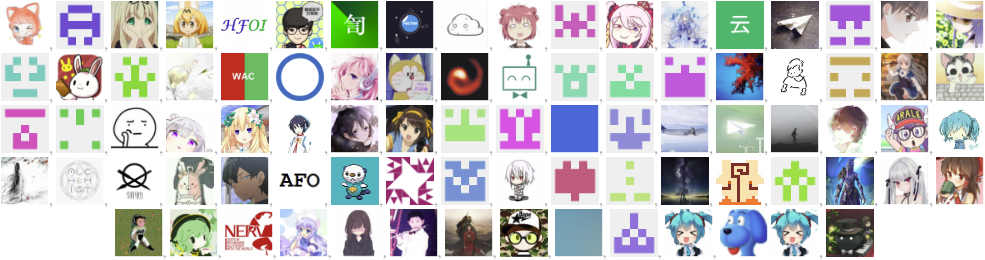
\includegraphics[width=0.9\textwidth]{contributors.png} 
  \caption{Contributors}
\end{figure}
\vskip 0.3 in

另外,也要特别感谢 \href{https://github.com/24OI}{24OI} 的朋友们的大力支持!

最后,感谢董小姐,让这一切成为可能。

\cleardoublepage
\setcounter{page}{1}
\tableofcontents
\cleardoublepage
\mainmatter
\setcounter{page}{1}
\chapter{简介}

\section{欢迎来到 \textbf{OI Wiki}。}

\begin{figure}[htbp]
  \centering
  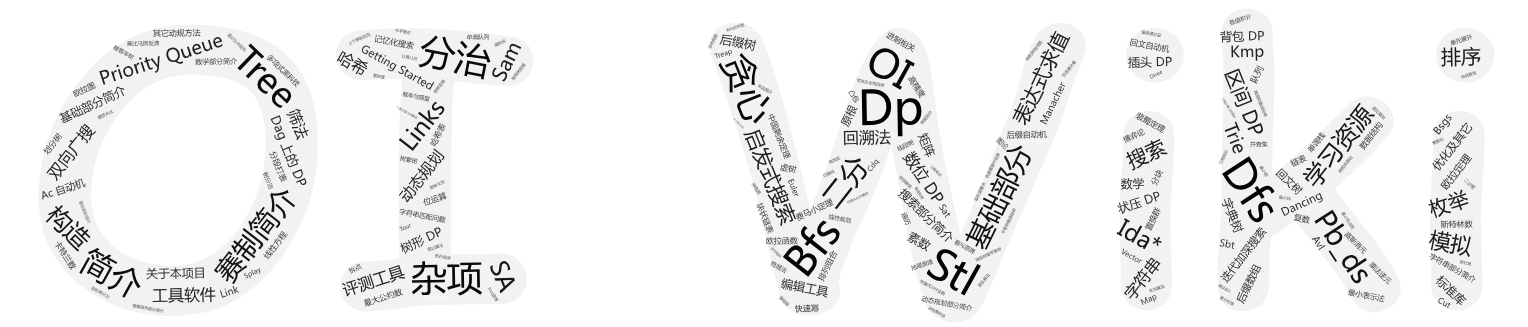
\includegraphics[width=0.7\textwidth]{docs/images/wordArt.png} 
  \caption{Word Art}
\end{figure}


\textbf{OI} (Olympiad in Informatics,信息学奥林匹克竞赛)在中国起源于 1984 年,是五大高中学科竞赛之一。自 1989 年起,每年还会选拔出国家集训队选手准备 IOI (International Olympiad in Informatics,国际信息学奥林匹克竞赛)。

\textbf{ICPC} (International Collegiate Programming Contest, 国际大学生程序设计竞赛)由 ICPC 基金会负责组织,是最具影响力的大学生计算机竞赛。ICPC 主要分为区域赛(Regional)和总决赛(World Finals)两部分。

\textbf{OI Wiki} 致力于成为一个免费开放且持续更新的知识整合站点,大家可以在这里获取关于 \textbf{编程竞赛 (competitive programming)} 有趣又实用的知识,我们为大家准备了竞赛中的基础知识、常见题型、解题思路以及常用工具等内容,帮助大家更快速深入地学习编程竞赛。

本项目受 \href{https://ctf-wiki.github.io/ctf-wiki/}{CTF Wiki} 的启发,在编写过程中参考了诸多资料,在此一并致谢。

本项目文档内容托管在 \href{https://github.com/24OI/OI-wiki}{GitHub},主要使用 \href{https://github.com/24OI/OI-wiki/issues}{Issues} / \href{https://jq.qq.com/?_wv=1027&k=5EfkM6K}{QQ} / \href{https://t.me/OIwiki}{Telegram} 进行交流沟通,期待你的加入。

Telegram 群组链接为 \href{https://t.me/OIwiki}{@OIwiki} , QQ 群号码为 \href{https://jq.qq.com/?_wv=1027&k=5EfkM6K}{588793226},欢迎加入。

\section{OI 赛制简介}

\subsection{赛事介绍}

OI 竞赛是一项全球的赛事,每年夏天会有世界级竞赛(IOI)举行,参赛选手大多都经过层层选拔。对于大部分选手而言,每年新赛季从 10 月的 NOIP (省级选拔赛)开始。

OI 竞赛中允许使用的语言包括 Pascal(NOI 将于 2020 年停止使用 Pascal,NOIP 将于 2022 年停止使用 Pascal),C 和 C++。其中 C++ 的版本不同考试有不同的规定。考试题目一般为算法或者数据结构相关的内容,题目形式包括传统题(最常见的规定输入和输出到文件的题目)和非传统题(提交答案题、交互题、补全代码题等等)。

\subsubsection{NOIP}

NOIP(National Olympiad in Informatics in Provinces)是全国青少年信息学奥林匹克联赛,顾名思义,是以省为单位排名评奖,对于大部分高校来说,获得省一等奖可以用于获得自主招生资格。

NOIP 分为初赛和复赛两个阶段。初赛会考察一些计算机基础知识和算法基础(笔试),复赛是上机考试,时间上一般是 11 月的第二个周末。全国使用同一套试卷,但是评奖规则是按照省内情况由 CCF (中国计算机学会)统一指定,并于赛后在 \href{http://www.noi.cn}{NOI 官方网站} 上公布。

\subsubsection{省选}

省队选拔赛是用于选拔各省参加全国赛的代表队,各个省队的名额有复杂的计算公式,一般和之前的成绩和参赛人数有关。省选由各个省自行决定,目前的趋势是很多省份选择联合命题。通常来讲,NOIP 分数需要在省选中占一定比例。

\subsubsection{NOI}

NOI(National Olympiad in Informatics)是全国信息学奥林匹克竞赛,一般在七月份举行,有现场赛和网络赛。现场赛选手分为四类,其中 A、B、C 类为正式选手。A、B 类对应省队的 A、B 类选手(其中 A 类在计算成绩时会有 5 分加分),C 类名义上是学校对 CCF 做出突出贡献后的奖励名额,D 类是邀请赛选手,如果成绩超过分数线的话,只有成绩证明而没有奖牌(同等分数含金量要低一些)。正式选手前 50 名组成国家集训队,获得保送资格。网络赛报名形式上没有门槛。

\subsubsection{WC}

WC(Winter Camp)是全国青少年信息学奥林匹克竞赛冬令营,是每年冬天在当年 NOI 举办地进行的一项活动,内容包括若干天的培训和一天的考试。这项考试主要用于从国家集训队( 50 人)选拔国家候选队( 15 人)。

\subsubsection{APIO}

APIO(Asia-Pacific Informatics Olympiad)是亚太地区信息学奥林匹克竞赛,CCF 每年会在五月初举办中国赛区镜像赛。在比赛日前后会有培训活动。

\subsubsection{CTSC}

CTSC(China Team Selection Competition)是中国队选拔赛。用来从国家候选队( 15 人)中选拔国家队( 6 人)准备参加当年夏天的 IOI 比赛,其中正式选手 4 人,替补选手 2 人。

注: APIO 和 CTSC 都是以省为单位报名,一般是按照 NOIP 成绩排序来确定谁会有机会参加 APIO 和 CTSC (二者一般时间上非常接近)。

\subsubsection{IOI}

IOI(International Olympiad in Informatics)是国际信息学奥林匹克竞赛,每个国家有四人参赛,比赛一般会有直播。IOI 赛制中每个题目会有 subtask (子任务),每个子任务对应一定的分数。

\subsection{赛制介绍}

\subsubsection{OI 赛制}

一般的 OI 赛制可以理解为单人在 5 个小时的时间内尝试解决 3 个题。每个题目可以不全部解决,会有多个数据点,题目的分数一般是数据点得分之和。每个数据点还可能会有部分分,就是数据点内部也不需要完全正确才能得到分数。评分方式是在比赛结束后统一评测,只有一次提交机会。

NOIP、NOI、省选都是 OI 赛制。

\subsubsection{IOI 赛制}

目前国内比赛也在逐渐向 IOI 赛制靠拢。

IOI 赛制可以赛时任意提交,可以即时查看评测结果, APIO、IOI 都是 IOI 赛制。

\subsubsection{ICPC 赛制}

在 ICPC 比赛中一般是三个人使用一台机器,每个题目只有在所有数据点全部正确后才能得到分数。比赛过程中可以有多次提交机会,实时评测并返回结果。比赛排名根据做题数和罚时来评判,罚时是通过题目的用时之和加上错误提交次数乘以一个系数。在 ICPC 相关赛事中,选手允许带纸质资料。

\subsubsection{Codeforces (CF) 赛制}

\href{https://codeforces.com}{Codeforces} 是一个在线评测系统,定期会举办比赛。它的比赛特点是在比赛过程中只测试一部分数据(pretests),而在比赛结束后返回完整的所有测试点的测试结果(system tests)。比赛时可以多次提交,允许 hack 别人的代码(此处 hack 的意思是提交一个测试数据,使得别人的代码无法给出正确答案)。当然,如果想要 hack ,必须要锁定自己的代码(换言之,比赛时无法重新提交该题)。

\subsection{其他国家和地区的 OI 竞赛}

\subsubsection{美国:USACO}

官网地址:\url{https://www.usaco.org/}

USACO 或许是国内选手最熟悉的外国 OI 竞赛(因此可能也是中文题解最多的外国 OI 竞赛)。  

每年冬季到初春,USACO 会每月举办一场网络赛。一场比赛持续 $3\sim5$ 个小时。  

根据官网的介绍,USACO 的比赛分成这 4 档难度(2015\textasciitilde{}2016 学年之前为 3 档):

\begin{itemize}
\item 铜牌组,适合编程初学者,尤其是只学了最最基础的算法(如:排序,二分查找)的学生。
\item 银牌组,适合开始学习基本的算法技巧(如:递归,搜索,贪心算法)和基础数据结构的学生。
\item 金牌组,学生会遇到更复杂的算法(如:最短路径,DP)和更高级的数据结构。
\item 铂金组,适合有着扎实的算法设计能力的选手,铂金组可以帮助他们以复杂且更开放的问题来\sout{放飞}挑战自我。
\end{itemize}

在国内,目前 USACO 题目最齐全的是洛谷。

\subsubsection{波兰:POI}

官网:\url{https://oi.edu.pl/}  

官方提交地址:\url{https://szkopul.edu.pl/p/default/problemset/}  

POI 是不少省选选手最常刷的外国 OI 比赛。  

根据(已经凉凉的)\url{http://main.edu.pl/en/} 的描述,POI 的流程如下:  

\begin{itemize}
\item 第一轮:五题,网络赛,公开赛。
\item 第二轮:包含一场练习赛,和两场正式比赛。
\item 第三轮:赛制同上。
\item ONTAK:POI 训练营(类似国内的集训队)
\end{itemize}

你可能还听说过 PA。PA 的大意是 “算法大战”(我也不知道为啥它叫这名字)。

目前在国内 OJ 中,POI 题目最全的是 BZOJ。

\subsubsection{克罗地亚:COCI}

官网地址:\url{http://www.hsin.hr/coci/}  

(有时候英文版的更新会延迟,克罗地亚语版本:\url{http://www.hsin.hr/honi/})

难度跨度很大的比赛,大约是从普及 - $\sim$ 省选 -。以往 COCI 所有的题目均提供题目、数据、题解和标程,然而从 2017 年底之后,COCI 的题解和标程就断更了(不是没有英语版翻译,而是连克罗地亚语的版本都没有)。

洛谷、BZOJ 和 LibreOJ 都有少量的 COCI 题目。

\subsubsection{日本:JOI}

官网地址:\url{https://www.ioi-jp.org/}  

日本信息学奥赛(日本情報オリンピック)一般简称为 JOI。JOI 所有的题目都提供题目、数据、题解和标程。近两年的 JOI 决赛和春训营提供了英语题面,但并没有英语题解。历年的 JOI Open 都提供了英语版题面和题解。绝大部分 JOI 题可以左转 AtCoder 提交。

JOI 的流程:

\begin{itemize}
\item 预赛(予選)
\item 决赛(本選 / JOI Final)
\item 春训营(春季トレーニング合宿 / JOI Spring Camp / JOISC)
\item 公开赛(通信教育 / JOI Open Contest)
\end{itemize}

目前 LibreOJ 和 BZOJ 有近些年的 JOI Final、JOISC 和 JOI Open 的题目。UOJ 有部分 JOISC 2017 的题目。

JOI Final 的难度在提高 - $\sim$ 提高 + 左右。JOISC 和 JOI Open 的题目的难度在提高 $\sim$ NOI - 不等。

你可以在 JOI 官网或者 AtCoder 上找到更多的 JOI 题 (日文题面)

\subsubsection{台湾地区:資訊奧林匹亞競賽}

台湾地区把 OI 中的 informatics 翻译成 “资讯” 而非大陆通用的翻译 “信息”。  

台湾地区的选手如果想去参加 IOI,需要经过这几场比赛的洗礼:  

\begin{itemize}
\item 區域資訊學科能力競賽
\item 全國資訊學科能力競賽
\item 資訊研習營(TOI)
\end{itemize}

\subsubsection{俄罗斯:ROI}

俄罗斯信息学奥赛(олимпиадная информатика)一般简称为 ROI。  

官网:\url{http://neerc.ifmo.ru/school/archive/index.html}  

在线提交地址:\url{https://contest.yandex.ru/roiarchive/}  

一般简称为 ROI。流程:

\begin{itemize}
\item 市级比赛(Municipal stage / Муниципальный этап)
\item 地区级比赛(Regional Stage / Региональный этап)
\item 决赛(Final Stage / Заключительный этап)
\end{itemize}

你可能已经在 Codeforces 上见过了一些 ROI 题。目前 LibreOJ 有近两年的 ROI 决赛题(包括翻译)。

\subsubsection{加拿大:CCC \& CCO}

CCC: Canadian Computing Competition  

CCO: Canadian Computing Olympiad  

官网地址:\url{https://cemc.math.uwaterloo.ca/contests/past_contests.html#ccc}  

CCC 提交地址:\url{https://dmoj.ca/problems/?category=4}  

CCO 提交地址:\url{https://dmoj.ca/problems/?category=24}  

CCC 在 DMOJ 有官方 (?) 题解。  

CCC Junior / Senior 贴近 NOIP 普及组 / 提高组难度。CCO 想要拿到金牌可能得有 NOI 银的水平。

\subsubsection{法国与澳大利亚:FARIO}

提交地址:\url{http://orac.amt.edu.au/cgi-bin/train/hub.pl}

FARIO 的题目与 NOI 的难度旗鼓相当。

\subsection{其它大洲级 OI 竞赛}

\subsubsection{BalticOI}

BalticOI 面向的是波罗的海周边各国。BalticOI 2018 的参赛国有立陶宛、波兰、爱沙尼亚、芬兰等 9 国。

除了 2017 年,BalticOI 每年都公开题面、测试数据和题解。然而 BalticOI 没有一个固定的官网,每年的主办方都会新建一个网站…… 关于历年的官网地址,Planet6174 整理出了一个\href{https://loj.ac/article/416}{帖子}。

目前 LibreOJ 有近十年的 BalticOI 题。

\subsubsection{BalkanOI}

BalkanOI 面向巴尔干地区周边各国。BalkanOI 2018 的参赛国有罗马尼亚、希腊、保加利亚、塞尔维亚等 12 国。

BalkanOI 只有某几年公开题面、测试数据和题解,官网地址参见上面那个帖子。

\subsubsection{CEOI}

CEOI 2018 的参赛国与上面两个比赛有部分重叠,包括波兰、罗马尼亚、格鲁吉亚、克罗地亚等国。

CEOI 每年都公开题面、测试数据和题解,官网地址参见上面那个帖子。

在国内 OJ 中,BZOJ 的 CEOI 题相对最齐。

\subsubsection{Nordic Olympiads in Informatics (NOI)}

官网地址:\url{http://nordic.progolymp.se}

近两年才开始举办的比赛,面向北欧各国。

\section{学习资源}

\subsection{在线测试 (训练) 平台}

在线测试平台又称 Online Judging System,一般用来刷题、组织比赛,也有的会提供博客功能方便选手交流。

\subsubsection{国内}

\begin{itemize}
\item \href{https://www.51nod.com/}{51Nod} (有很多好的数学题和思维题)
\item \href{https://www.lydsy.com/JudgeOnline/}{BZOJ} (优质的题巨多)
\item \href{http://www.codevs.cn/}{CodeVS}
\item \href{http://acm.fzu.edu.cn/}{FZUOJ} (福州大学)
\item \href{http://acm.hdu.edu.cn/}{HDU OJ} (杭电的 OJ,多校训练的题目放在这里)
\item \href{https://hihocoder.com/}{hihoCoder}
\item \href{https://www.jisuanke.com/}{计蒜客}
\item \href{https://duck.ac/}{Judge Duck Online} (松松松的 OJ,精确到 $\mu s$)
\item \href{http://www.joyoi.cn/}{JoyOI} (原 Tyvj)
\item \href{https://loj.ac/}{LibreOJ}
\item \href{http://www.luogu.org/}{洛谷} (常用 OJ,现代 OJ 支持发布比赛等很多功能,评测机快)
\item \href{https://www.nowcoder.com/}{牛客网}
\item \href{http://openjudge.cn/}{OpenJudge}
\item \href{http://poj.org/}{POJ} (PKU OJ,国内历史最悠久的 OJ 之一,很多英文题,有一些基础题和好题)
\item \href{http://uoj.ac/}{Universal OJ} (VFK 的 OJ,多原创比赛题和 CCF/THU 题 难度较高)
\item \href{https://vijos.org/}{Vijos}
\item \href{https://vjudge.net/}{Virtual Judge} (可以方便的在 Vjudge 上提交别的 OJ 的题,尤其是一些国内不太方便的 OJ)
\item \href{http://acm.zju.edu.cn/onlinejudge/}{ZOJ} (浙大)
\end{itemize}

\subsubsection{国外}

\begin{itemize}
\item \href{https://atcoder.jp/}{AtCoder} (日本的一个 OJ,类似 Codeforces 但是也会放 JOI 的题)
\item \href{https://codechef.com/}{CodeChef} (印度 OJ,周期性有比赛)
\item \href{https://codeforces.com/}{Codeforces} (俄罗斯 OJ,有很多比赛)
\item \href{https://csacademy.com/}{CS Academy}
\item \href{https://dmoj.ca/}{DMOJ} (加拿大开源的 OJ,语言支持广;题库是各大比赛的存档,也有定期自行举办的比赛)
\item \href{https://www.hackerrank.com/}{HackerRank} (有很多比赛)
\item \href{https://open.kattis.com/}{Kattis}
\item \href{https://leetcode.com/}{LeetCode} (有中文分站:\href{https://leetcode-cn.com/}{LeetCode China})
\item \href{http://www.spoj.com}{SPOJ}
\item \href{https://www.topcoder.com/}{Topcoder} (有很多比赛)
\item \href{http://acm.timus.ru/}{Ural}
\item \href{https://uva.onlinejudge.org/}{UVa} (做 lrj 的书怎么可能不知道这个 OJ)
\item \href{https://contest.yandex.ru/}{Yandex} (存档了近几年的全俄罗斯信息学奥赛)
\item \href{http://lightoj.com}{Light OJ}(一个快挂了的 OJ,\texttt{www}域名无法访问,请使用\href{http://lightoj.com}{根域名}访问)
\end{itemize}

\subsection{教程}

\begin{itemize}
\item \href{https://oi-wiki.org}{OI Wiki}
\item \href{http://codeforces.com/blog/entry/57282}{Codeforces 上网友整理的一份教程合集}
\item \href{https://cp-algorithms.com/}{英文版 E-Maxx 算法教程}
\item \href{http://www.csie.ntnu.edu.tw/~u91029/}{演算法笔记} 台湾师范大学总结的教程
\item \href{https://algo.is/t-414-aflv-competitive-programming-course-2016/}{algo.is}
\item \href{http://web.stanford.edu/class/cs97si/}{CS 97SI: Introduction to Programming Contests} 斯坦福的一门课
\item \href{https://www.geeksforgeeks.org/how-to-prepare-for-acm-icpc/}{如何为 ACM-ICPC 做准备? - geeksforgeeks}
\end{itemize}

\subsection{书籍}

\begin{itemize}
\item 信息学奥赛一本通 (初学者向)
\item 算法竞赛入门经典 (人称紫书)
\begin{itemize}
\item \href{https://github.com/sukhoeing/aoapc-book/}{第一版 配套资源仓库 (mirror)}
\item \href{https://github.com/aoapc-book/aoapc-bac2nd}{第二版 配套资源仓库}
\item \href{https://github.com/sukhoeing/aoapc-bac2nd-keys}{第二版 习题选解}
\end{itemize}
\item 算法竞赛入门经典——训练指南 (人称大白)
\item 算法艺术与信息学竞赛 (人称黑书)
\item 算法竞赛进阶指南
\begin{itemize}
\item \href{https://github.com/lydrainbowcat/tedukuri}{配套资源仓库}
\end{itemize}
\item 具体数学
\item \href{https://cses.fi/book/index.html}{Competitive Programmer's Handbook}
\item 算法导论
\begin{itemize}
\item \href{https://github.com/walkccc/CLRS}{答案解析 (English)}
\end{itemize}
\item 啊哈算法
\item 挑战程序设计竞赛全套 (通俗易懂)
\item 算法概论 (提纲挚领,但内容较少)
\item \href{http://www.legend-k.com/Algorithm/Algorithm.pdf}{Legend-K 的数据结构与算法的笔记}
\end{itemize}

\subsection{工具}

\begin{itemize}
\item \href{https://visualgo.net/en}{经典算法的可视化结果 - VisuAlgo}
\item \href{https://www.cs.usfca.edu/~galles/visualization/}{算法可视化 - USF}
\item \href{https://oeis.org}{OEIS 整数数列搜索引擎}
\item \href{https://paste.ubuntu.com}{Ubuntu Pastebin,可以用来分享代码}
\item \href{https://www.udebug.com}{uDebug 提供一些 OJ 题目的调试辅助}
\item \href{https://zh.cppreference.com/w/}{提供 C++ 内语法的查询等 - cppreference.com}
\item \href{https://csacademy.com/app/graph_editor/}{图论画板} (同时推荐 GraphViz)
\item \href{http://www.mohu.org/info/symbols/symbols.htm}{LaTeX 数学公式参考}
\item \href{https://godbolt.org/}{Godbolt - 在浏览器中查看编译后代码块对应的汇编语句}
\item \href{https://github.com/hellogcc/100-gdb-tips}{《100 个 gdb 小技巧》}
\item \href{https://mathpix.com/}{截图转 LaTeX - Mathpix}
\end{itemize}

\subsection{题集}

\begin{itemize}
\item \href{http://blog.csdn.net/skywalkert/article/details/46594541}{POJ 训练计划}
\item \href{http://train.usaco.org/usacogate}{USACO}
\item \href{https://www.luogu.org/training/mainpage}{洛谷试炼场}
\item \href{https://codeforces.com/blog/entry/55274}{-Morass- 贴在 Codeforces 上的一份题单}
\item \href{https://vjudge.net/article/446}{北京大学暑期课课件例题}
\end{itemize}

\section{常见错误}

本页面主要分享一下在竞赛中经常 / 很多人会出现的错误。

\begin{enumerate}
\item 由于运算符优先级产生的错误。
\begin{itemize}
\item \texttt{1 << 1+1} : 1 左移了 2,即该表达式返回的值是 \texttt{4}。
\item 由于宏的展开,且未加括号导致的错误:
\begin{cppcode}
#define pwr(x) x* x
pwr(2 + 2)
\end{cppcode}
该宏返回的值并非 $4^2 = 16$ 而是 $2+2\times 2+2 = 8$。
\end{itemize}
\item 文件操作有可能会发生的错误。
\begin{itemize}
\item 对拍时未清除文件指针即 \texttt{fclose(fp)} 就又令 \texttt{fp = fopen()}, 这会使得进程出现大量的文件野指针。
\item \texttt{freopen()} 中的文件名未加 \texttt{.in}/\texttt{.out}。
\end{itemize}
\item \texttt{int mian()}。
\item 无向图边表未开 2 倍。
\item 多组数据未清空数组。
\item 输出\texttt{double}要使用 \texttt{\%f} 而非 \texttt{\%lf}。 参考 \href{https://stackoverflow.com/questions/4264127/correct-format-specifier-for-double-in-printf}{链接}
\item 分治未判边界导致死递归。
\item 读入优化未判断负数。
\item 不正确地使用 \texttt{static} 修饰符。
\item \texttt{-1 >> 1 == 1}
\item 不正确地使用宏。
\texttt{\#define min(x,y) x<y?x:y} 如果这里的 \texttt{x} 或 \texttt{y} 是表达式,会被重复计算
\item 一些 OJ 上选择 \texttt{c++} 和 \texttt{g++} 提交得到的结果可能会不一样
\end{enumerate}

\section{常见技巧}



  \section{评测工具}
  
很多时候,你拿到了一套题,想要在本地测试一下自己能得多少分,这时候就需要评测软件了。

\subsection{Cena}

Cena 是由刘其帅和李子星使用 Pascal 语言编写的开源评测工具,是流传最广泛的本地评测工具。Cena 最初开源于 Google Code 平台,由于不明原因 Google 删除了 Cena 项目,目前可以在 \href{https://web.archive.org/web/20131023112258/http://code.google.com/p/cena/}{Web Archive} 上找到 Cena 的官网。

Cena 的源代码可以在\href{https://github.com/billchenchina/cena}{这里}找到。

Cena 对权限的限制不是很明确,测试的时候可以读测点 AC QAQ

\subsection{Lemon}

Lemon 是 zhipeng-jia 写的开源的评测工具,地址在:\href{https://github.com/zhipeng-jia/project-lemon}{zhipeng-jia/project-lemon}。

Ir1d 提供了一份 linux 下编译好的版本在 \href{https://github.com/FreestyleOJ/Project_lemon/tree/Built}{FreestyleOJ/Project\textbackslash{}\_lemon}。

Menci 提供了一份更新的版本在 \href{https://github.com/Menci/Lemon/}{Menci/Lemon}。

\textbf{注意} macOS 下 Lemon 可能会出现内存测试不准确的情况, 这是由于 mac 下没有一些 Linux 的监测工具,而 Lemon-Linux 也没有对于 macOS 的使用优化。

\subsubsection{自行编译}

在 Ubuntu 下编译:

\begin{minted}{bash}
sudo apt update
sudo apt install qt5-default build-essential git -y
git clone --depth=1 http://github.com/menci/lemon.git
cd lemon
# 可以修改 make 文件来调整 make job 的线程数
sed -i 's/make $/make -j 1 $/g' make
./make
cp Lemon ~
cd ..
\end{minted}

\subsubsection{数据格式}

首先打开 lemon 选择新建试题,而后打开新建试题的文件夹

题目和数据应该如以下格式所示

\begin{minted}{text}
├── data
│   ├── gendata.py
│   ├── product
│   │   ├── product100.in
│   │   ├── product100.out
│   │   ├── product10.in
│   │   ├── product10.out
│   │   ├── product11.in
...
\end{minted}

当所有试题添加完成后,回到 lemon 选择自动添加试题

此时你的题目和数据点应该都显示在 lemon 当中了

\subsection{Arbiter}

Arbiter 为北京航空航天大学为 NOI Linux 开发的评测工具,现已用于各大 NOI 系列程序设计竞赛的评测。据吕凯风在 2016 年冬令营上的讲稿《下一代测评系统》,Arbiter 是由北京航空航天大学的团队(貌似叫 GAIT)在尹宝林老师的带领下开发完成的。不过该测评工具在开发完成后就一直没有维护与更新,导致测评体验极差,和 NOI Linux 自带的 GUIDE 一样沦为选手与教练疯狂吐槽的对象。但是 NOIP 与 NOI 的题目测评是在 Arbiter 下进行的,因此仍然需要了解 Arbiter 的使用方法。

\subsubsection{使用方法}

首先准备好选手源程序文件夹。选手文件夹如 NOIP 格式创建:

\begin{minted}{text}
players/
| -- <contestant_1's ID>
|     | -- <problem_1>
|     |   `-- <problem_1>.c/cpp/pas
|     | -- <problem_2>
|     |   `-- <problem_2>.c/cpp/pas
|     | ...
|     | -- <problem_x>
|        `-- <problem_x>.c/cpp/pas
| -- <contestant_2's ID>
|     | -- <problem_1>
|     ...
...
\end{minted}

其中,\texttt{<contestant\_x's ID>} 指的是选手编号,形如 \texttt{<省份>-< 编号 >},例如 HL-001,JL-125 等等,\texttt{<problem\_x>} 指的是题目名称。

当然,在自测时可以使用字母,短线(即 \texttt{-})和数字的组合作为选手编号。

准备好选手文件夹还不够,需要准备选手名单。名单格式如下:

\begin{minted}{text}
<contestant_1's ID>, <contestant_1's name>
<contestant_2's ID>, <contestant_2's name>
...
\end{minted}

其中 \texttt{<contestant\_x's name>} 表示选手姓名,保存这个文件为纯文本文件,文件编码是 GB2312。

当然也可以手动添加,稍后介绍。

这样的话,选手源程序文件夹已经搞定,现在配置数据。

每组数据的命名格式如下:

\begin{minted}{text}
<problem_x><y>.in <problem_x><y>.ans
\end{minted}

其中,\texttt{<y>} 是数据编号,编号从 1 开始。

默认测试数据后缀名是 \texttt{.ans},选手输出的后缀名是 \texttt{.out},不能混淆。不用将每题的测试数据放置在各自文件夹里,只需要放在一起即可。

这样就准备好了,现在开始测评文件夹的配置。

工具栏 - 应用程序 - 编程 - Arbiter 测评系统,启动 Arbiter。

\begin{figure}[htbp]
\centering
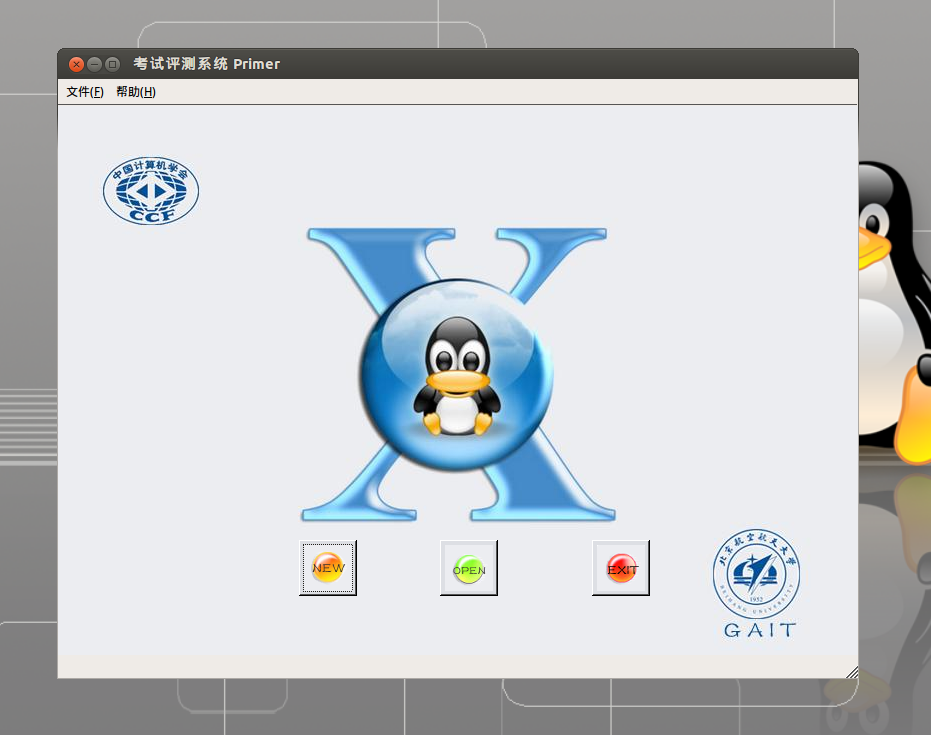
\includegraphics[width=0.7\textwidth]{docs/intro/images/arbiter_home.png} 
\caption{Arbiter\_Home}
\end{figure}

如果要打开已经建立的比赛,请点击 OPEN,这里新建一个竞赛,选择 New,设置一下名称和比赛目录即可。

注意,需要新建一个文件夹,然后选择其为比赛目录。

\begin{figure}[htbp]
\centering
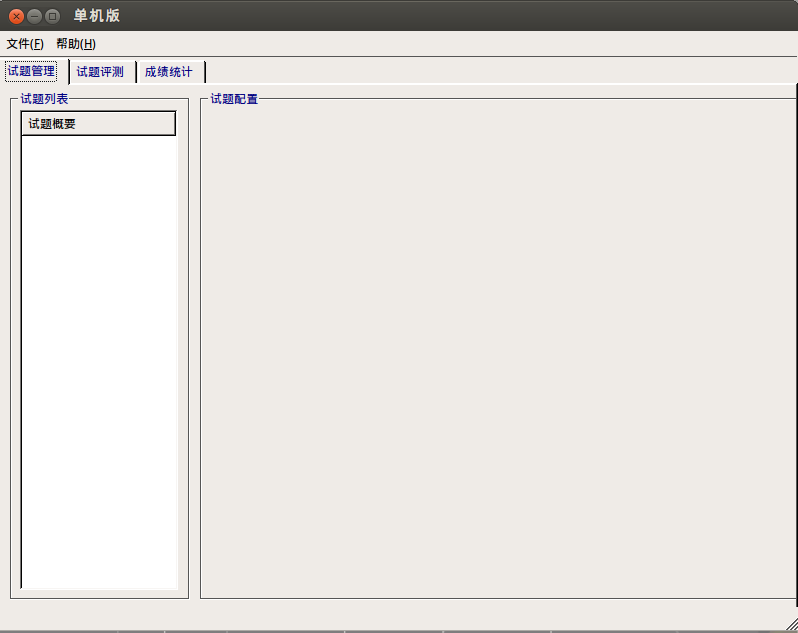
\includegraphics[width=0.7\textwidth]{docs/intro/images/arbiter_addproblem.png} 
\caption{AddProblem}
\end{figure}

在左边试题概要里右键 - 添加考试,再在考试标签上右键 - 添加试题,新建出试题即可。

单击考试左边的 \texttt{+} 即可全部显示,单击试题标签对试题名称进行修改,改为题目的英文名称,同时修改题目时间与空间限制和比较方式。比较方式十分不推荐用全文完全直接比较,对于 Windows 下制作的数据十分不友好。比较方式不选的话默认为字符串比较中的单行单字符串比较方式。如果测试数据不同的话一定要注意比较方式的选择!

\begin{figure}[htbp]
\centering
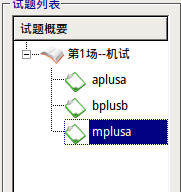
\includegraphics[width=0.7\textwidth]{docs/intro/images/arbiter_problem.png} 

\end{figure}

(建了一些无聊的问题)

这一步\textbf{十分重要:}点击文件 - 保存!一定要保存,否则没有题目配置文件!每一次对题目配置的修改都要保存!

此时,打开考试文件夹,会发现有如下内容。

\begin{minted}{text}
<name>/
| -- data
| -- evaldata
| -- filter
| -- final
| -- players
| -- result
| -- tmp
`-- day1.info
`-- player.info
`-- setup.cfg
`-- task1_1.info
`-- task1_2.info
`-- task1_3.info
`-- team.info
\end{minted}

我们把已经建好的选手程序文件夹放在 \texttt{players/} 目录下,将所有测试数据(不放在文件夹里)放在 \texttt{evaldata} 中。

\texttt{filter/} 文件夹放置了一些比较器及其源代码,写自定义比较器时可以参考,\texttt{result/} 文件夹存放选手的测评结果,\texttt{tmp/} 文件夹是测评时文件夹。

配置好后,就是正式测评环节了。点开 “试题评测” 标签,然后会出现如下所示情况。

\begin{figure}[htbp]
\centering
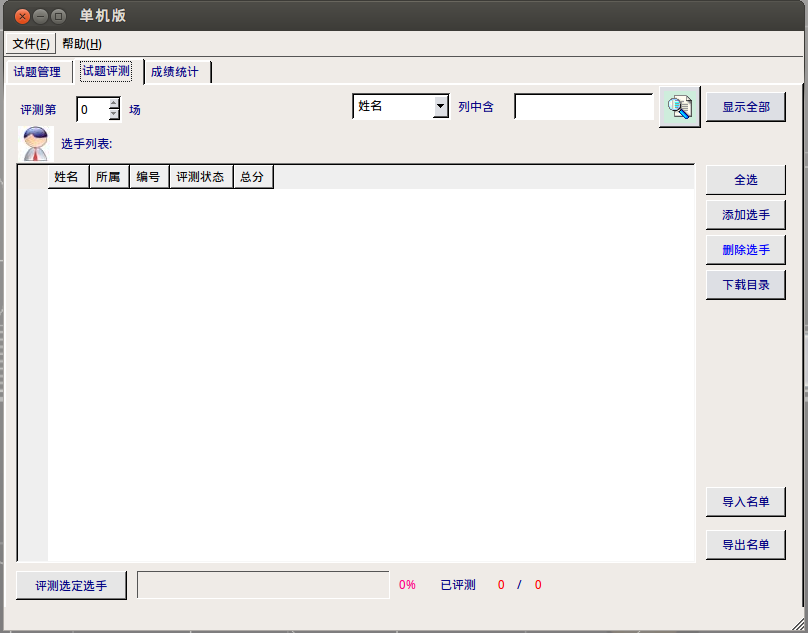
\includegraphics[width=0.7\textwidth]{docs/intro/images/arbiter_pretest.png} 
\caption{Pretest}
\end{figure}

如果已经建立好选手名单了,选择右边的导入名单进行导入。如果人数较少,可以选择右边的添加选手进行导入。

导入好后是这样的。

\begin{figure}[htbp]
\centering
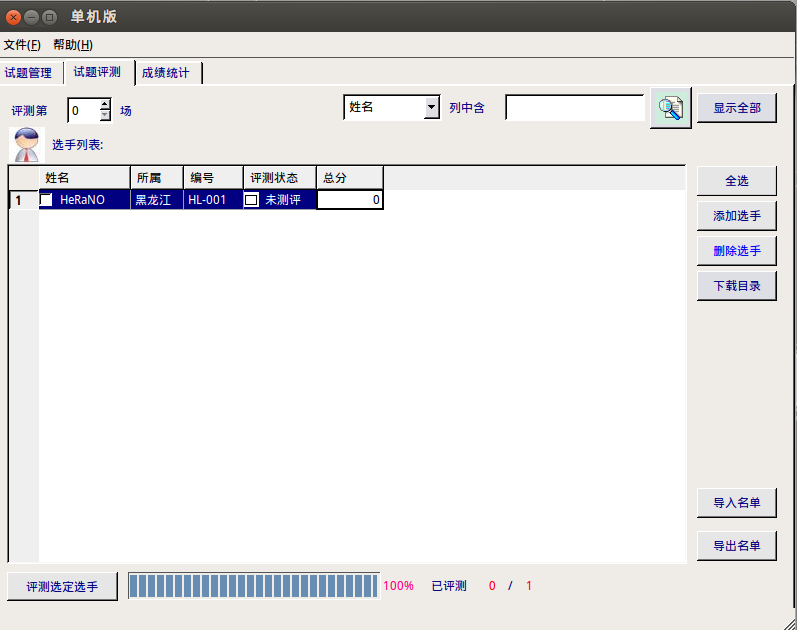
\includegraphics[width=0.7\textwidth]{docs/intro/images/arbiter_test.png} 
\caption{Test}
\end{figure}

因为我取得编号是 \texttt{HL-001},所以会自动识别出 “所属” 一栏。如果不是 NOIP 规范的编号是识别不出来的。

这个时候,要用\textbf{向上箭头}把测评第 0 场变为测评第 1 场,如果直接修改的话会识别失败。

然后选择右边的全选,再选择下面的评测选定选手,选择要测评的题目(有全部试题),等待测评结束即可。

\subsubsection{注意事项,槽点}

\paragraph{自定义校验器的编写}

注意编译后自定义校验器名称为 \texttt{<problem>\_e},其中 \texttt{<problem>} 为题目名称,必须放在 \texttt{filter/} 文件夹下。在配置题目时选择自定义校验器,然后选择需要的自定义校验器。

可以参考 \texttt{filter/} 下的源代码编写。

\paragraph{测评时注意事项}

以下信息均来自敝校教练。

据说很容易死机,需要注意。

据说大量测评时移动鼠标会导致死机,需要注意。

据说不定时闪退,和 Anjuta 一样,需要注意。

据说配置时需要注意权限问题(但是我并未遇到)。

……

\paragraph{诶我怎么只能看见代码不能看见每个点得多少分}

测试点详细信息需要在 \texttt{result/} 文件夹下查看,文件夹下会有选手的结果文件夹,结果文件的后缀名为 \texttt{.result},用纯文本方式查看即可。

\sout{(我觉得这个设计很值得吐槽)}

\paragraph{诶这个测评系统好难看}

我觉得也是……

\paragraph{诶怎么测提交答案题啊}

在试题管理中题目配置的地方,将提交方式由源代码改为答案文件。然后选择自定义校验器即可。

\paragraph{诶这个测评系统有没有漏洞}

至少不能读取答案文件……

\texttt{bits/stdc++.h} 测得可用。

\texttt{\#pragma G++ optimize("O2")} 竟然可用。

\texttt{\_\_attribute\_\_((\_\_optimize\_\_("-O2")))} 竟然也可用。

我可能用的是假 Arbiter……

\paragraph{吐槽}

讲个故事:

有一天,一位竞赛教练在用 GUIDE 的时候发现单步调试功能出现了 Bug,于是他致信北航相关项目负责人询问解决办法,得到的回复是:“这个项目已经停止更新了。”

希望一个成熟的线下测评系统早日实现……

\subsection{CCR-Plus}

一款开源的界面好看的评测工具 GitHub 地址 :\href{https://github.com/sxyzccr/CCR-Plus}{sxyzccr/CCR-Plus}

  \section{编辑工具}
  
\subsection{Vim -- 编辑器之神}

\subsubsection{历史与争端}

Vim 的前身是 vi,一个简洁但是略有不足的编辑器,但是从 vi 开始,编辑器的模式区分和唯快不破的思想就已经体现的很到位了。Vim 即是 vi improved,是在 vi 原本所有的方式上进行的进一步提升,但是并不会改变 vi 的其他本质,只是增加了更多适应如今需要的一些功能。

vi 于 1976 年诞生,与 Emacs 不分先后,两者因其快捷的编辑被奉为神器,甚至使用者们还有爆发过 “圣战”,即是 \texttt{神的编辑器 Emacs} VS \texttt{编辑器之神 Vim},但是当然分不出结果,因为各有优劣。但它们共有的特点就是高度的扩展性与高度的可定制性以及快捷方便的使用。

Vim 的模式区分是一个很有意思的设定,普通模式与插入模式是最主要常用的模式,普通模式下的每个键都是命令,这便是 Vim 不同于 Emacs 的地方,若是习惯了 Vim 的模式之间的切换,大部分都是单个键的命令必然比 Emacs 的无限 Ctrl 会更高效,虽然 Vim 的小容量注定比不了 Emacs “操作系统” 这个东西那么万能,但是论快而言,Vim 是无可争议的顶尖编辑器。

Vim 有丰富的插件扩展,这点显然是比配置更迷人的存在。有这些扩展性存在,Vim 成为一个 IDE 也不会是不可能的事情。

但是,Vim 的初始学习注定是艰难的,因为其与多数主流操作不同的方式令稍懒的新手望而却步,这需要时间来适应但当度过最开始的不适应期之后,Vim 就再无难度,你会慢慢上瘾,不断优化你的配置,寻找新的更好用的插件。开始的过程就像是铸剑,之后的过程就像是与剑的更好的磨合,然后在剑中逐渐注入你的灵魂,这样它就成为了你最好的利器,令你无法割舍。乃至你会自己写适合自己的插件,就像是自创剑法,而不像是从别人那里借来剑法,杂七杂八融为一炉。

有人说了这样一句话:

Vim 是一款非常优秀的文本编辑器,但由于其陡峭的学习曲线,很多人还没开始学就放弃了,所以他们无法领悟 Vim 唯快不破的设计思想和精巧的使用体验。

附一张图,论各大编辑器的学习曲线,纵坐标代表掌握知识量及难度,横坐标代表使用的熟练程度与完成任务的效率。我们可以看到,Vim 的曲线岂止陡峭,都垂直了…… 但是开始过去后,是平稳的提升,只要度过开始的阶段,Vim 的学习将再无阻碍,一路直上有没有。

\begin{figure}[htbp]
\centering
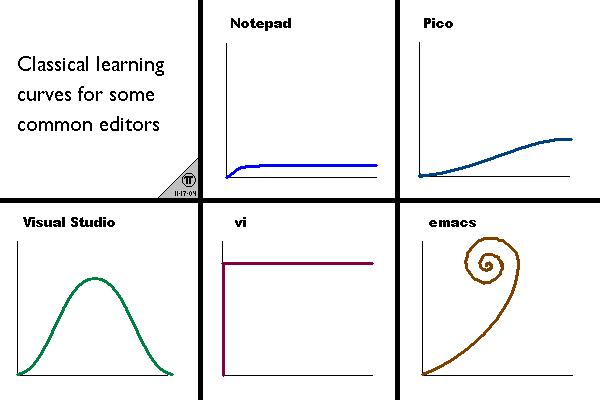
\includegraphics[width=0.7\textwidth]{docs/intro/images/horrorstories.jpg} 

\end{figure}

\subsubsection{安装}

一般的话,Linux 系统都是会自带 Vim 的,打开终端输入 \texttt{vim} 即可启用。

Vim 依附于终端,所以调整终端设置也可以达到美化效果。

但是自带的 Vim 很容易有功能残缺,比如有的就不能与系统剪切板交互 (将会在进阶篇讲解),各种未开启支持。那么这时候我们就需要手动安装,方法有二。第一步先是卸载 Vim,命令如下:

\begin{minted}{shell}
sudo apt-get remove vim
\end{minted}

然后安装有两种做法,一是使用命令安装,但我无法确定软件源的版本有没有问题 = =。

\begin{minted}{shell}
sudo apt-get install vim
\end{minted}

做法二,先到 \href{https://github.com/vim/vim/releases}{Releases - vim/vim} 下载源码包,然后解压,并进入解压后的文件夹,并打开终端,cd 至文件夹路径,并依次输入如下命令:

\begin{minted}{shell}
./configure
make
sudo make install
\end{minted}

make 的过程可能稍久,淡定点等。

最后在终端输入

\begin{minted}{shell}
vim
\end{minted}

就跳出了那个帮帮乌干达的可怜儿童啥的,按 \texttt{a} 或 \texttt{i} 键开始编辑新文件吧。

或者要打开某个文件的话就可以在终端中

\begin{minted}{shell}
vim 文件路径
\end{minted}

可以直接编辑文件。

\subsubsection{编译}

编译的话,先要安装 g++,命令如下:

\begin{minted}{shell}
sudo apt-get install g++
\end{minted}

然后 cd 至 cpp 文件指定路径执行如下命令

\begin{minted}{shell}
g++ filename.cpp -o filename
./filename
\end{minted}

第一个命令是编译,第二个则是运行。

一键编译运行的配置在配置篇给出。

\subsubsection{基础篇}

分模式来吧。

\paragraph{插入模式 (insert)}

插入模式的知识点其实没有太多,输入才是主职是伐。

首先,从普通模式如何进入插入模式呢?有数个命令:\texttt{i} 与 \texttt{a} 与 \texttt{A} 与 \texttt{o}。前两个差别不大,\texttt{i} 是在光标当前位置进行写代码,\texttt{a} 是往后挪一个字符写代码。\texttt{A} 是移动到当前行尾进行插入,\texttt{o} 是在行尾添加换行符并在下一行插入。

而如何返回普通模式?当然是 Esc 啦。但是,Vim 的插入与普通模式切换异常频繁,而 Esc 又太远了,有什么办法呢?Vim 还提供了 Ctrl + \textbackslash{}[ 的快捷键来返回普通模式,是否近多了呢?

虽说能够熟练了后,切换模式不再是问题,但是其实有的时候我们只是需要进入普通模式下按一次小命令,来回切换又显得浪费了一点点时间。而 Vim 又提供了插入 - 普通模式来避免这一尴尬的问题。在插入模式下,只需要按 Ctrl + o 即可进入此模式,当进行完一次操作后又会自动回到插入模式。这样岂不是更省时间?

\paragraph{普通模式 (normal)}

Vim 的命令大部分都是在普通模式下完成的,普通模式下可不能乱按,可以说每个键都是命令。

\begin{minted}{text}
首先是 hjkl 四个方向键。                         
                                              k ^
                                           h <     > l
                                                v j
\end{minted}

其实大多数编辑器都是用方向键做出移动命令,Vim 也不例外,但 \texttt{hjkl} 给了我们更好的选择,只需要一段时间的适应,你便能快速地操作它们进行移动,而且它们可没有方向键那么远,节省时间是一流的。

普通模式下最重要的命令,没有之一,那就是 \texttt{u}。撤销命令,作用是撤销上一次对文本的更改,普通模式下的 \texttt{x},\texttt{d},\texttt{p} 命令都会被撤销,同时进入一次插入模式所编辑的文本也算一次更改,\texttt{u} 命令会删去从进入到退出插入模式所输入的所有东西。与之对应的是 Ctrl + r 命令,他的作用是撤销上次的撤销命令,相当于大部分 windows 下程序中的 Ctrl + y。

然后的话, 就是普通模式下常用的命令。由于对行命令的使用很频繁,所以大部分的单键命令都可以通过按两次来实现对行操作。常用命令是 \texttt{x} ,用于删除光标后的一个字符。然后是 \texttt{d} 命令,也是删除,但是种类更多,这里不做赘述。同时 \texttt{d} 命令像之前说的,按两次即可删除整行,即 \texttt{dd}。

然后是\texttt{y}命令,可以复制被选中的区域,这涉及到可视模式,即按 \texttt{v} 进入可视模式,多用于选中区域。进入可视模式后移动光标来确定选取范围是可以的,此时按 \texttt{o} 键即可切换活动端,省去了如果跑反方向的麻烦。当然,我相信很多人还是习惯用鼠标操作这一过程的,包括移动光标。Vim 很温馨的提供了这一配置:\texttt{set mouse=a}。你可以将它写入你的配置文件中去。有了它之后,你将能够用鼠标选中区域并进行复制操作。当然,选中后按 \texttt{x} 或 \texttt{d} 亦可删除。同时,\texttt{y} 也符合 \texttt{d} 的性质,\texttt{yy} 将可以复制当前行。

然后就是更快的跳跃了。如果说只是使用 \texttt{hjkl} 的话,光标的移动显然不够快,而鼠标却又要伸手去拿。Vim 提供了普通模式下更快的跳跃方法,\texttt{w} 可以跳到下个单词的开头,而 \texttt{e} 可以跳到当前单词结尾,\texttt{0} 可以跳至行首,\texttt{\$} 可以跳至行尾,岂不是快多了?而且 \texttt{w},\texttt{e},\texttt{0},\texttt{\$} 还可以用于许多命令中 \texttt{de},\texttt{dw},\texttt{d0},\texttt{d\&} 分别对应删至单词尾,删至下个单词头,删至行首,删至行尾。以及\texttt{y}命令亦可同理。

然后是 Vim 的可重复。在输入某个命令前,输入一个数字的话,就会重复那么多次。如在普通模式下:

\begin{minted}{text}
asdasdasdasdasd
asdadasdddd
asdasdasd
\end{minted}

光标正位于第一行,该如何删除这三行呢?普通模式下按  \texttt{3 dd}  即可。其实还有\texttt{.}命令也是可以做到一些重复的,这会在效率篇中提到。

然后是全文的跳跃,按 \texttt{gg} 可跳至代码的开头,按 \texttt{G} 可跳至代码最后一行,先按数字再按 \texttt{G} 可跳至指定行。

那么在文中还有极为方便的查找功能,普通模式下只需按 \texttt{/} 下方即会出现查找框框,输入需要查找的字符按回车就好啦,如果有多个查找结果,只需按 \texttt{n} 即可跳至下一个查找处,按 \texttt{N} 即可跳至上一个。

常用命令大概就这些了……

\paragraph{命令行模式}

其实这并不能称作是一个模式 = =。

普通模式下只需要按 : 下方就会蹦出命令框框,输入相关命令即可。如 Vim 在线帮助文档,输入 \texttt{:help} 即可,如果看不懂英文…… 请下载 Vim 用户手册中文,或者移步插件篇。

此模式下有一些很有用的命令

\texttt{:q} 退出,\texttt{:w} 保存,\texttt{:wq} 保存并退出,\texttt{:q!} 不保存并退出,\texttt{:e filename} 打开当前目录下指定文件,这些是比较基础的。

然后是很强大的命令 \texttt{:x1,x2 s/A 串 / B 串 /} 作用是把第 \texttt{x1} 行至 \texttt{x2} 行中的所有 A 串替换成 B 串。想象一下题写完了,但是发现没开 \texttt{long long} 的时候,完全不绝望有没有,一个小命令,妙不可言。瞬间所有 \texttt{int} 变 \texttt{long long}。

以上都是 Vim 内部的命令,但是实际上如果命令形式是 \texttt{:! 命令} 那么就将在外部执行命令,即是以 bash 终端执行命令。既然都是外部 bash 了我就不多做介绍了,那块地不归我管……

\paragraph{可视模式}

可视模式的作用总结起来大概就是选中高亮,但是块状的可视模式可以干更多的事情,不过太麻烦了,对于新人来说大概会脑阔疼。

普通模式下按 \texttt{v} 即可进入可视模式,\texttt{hjkl} 可以移动高亮选区某一头,如果发现反了或者你进入可视模式的时候是在想要选中区域的中间位置,不用急着退出重进,更不用花时间又移回去,只需要按\texttt{o}即可切换活动端,操作高亮选区的另一头。或者用鼠标也不是不行啦……

用鼠标选中高亮选区当然也可以说是进入可视模式的办法之一。

然后就是\texttt{y}或者\texttt{d}操作,没了 QwQ。

emm 基础应该就用到这些了吧,往后的插件,配置,更多操作在对应篇幅里。

最后其实 Vim 还有一些基础操作,它们在 Vim 自带的教程里将会讲述。打开终端输入:

\begin{minted}{shell}
vimtutor
\end{minted}

即可进入教程,二三十分钟你就能掌握基础了,但应当加以练习才能彻底掌握。

\subsubsection{插件篇}

基础篇里说过,Vim 与 Emacs 之所以能成为两大巅峰的神器是因为其高度的扩展与可定制性,而最能体现这一特性的就是插件了。它们是最有魅力的一部分,是最令你无法抗拒的组成。

虽然考场上基本上不能用插件,但是日常的学习中,插件将对你的效率有很大的提高,而且一些插件的部分功能可以通过 Vim 自带实现以及配置实现。

首先,其实从前插件的安装必须下载之后丢到 .vim 文件夹中,删了又要下云云,十分麻烦。于是在使用者们的捣鼓下,一枚强大的插件管理器由此诞生——Vundle。

当然你的配置里必须有如下两行:

\begin{minted}{vim}
set nocompatible
filetype plugin on
\end{minted}

以确保你的 Vim 可以加载插件,哪怕是 Vim 原生内置的插件也需要的。

至于具体过程如下:

首先是在 home 目录下建立文件夹 .vim。然后打开终端输入以下命令:

\begin{minted}{shell}
sudo apt-get install git
git clone https://github.com/VundleVim/Vundle.vim.git ~/.vim/bundle/Vundle.vim
\end{minted}

就安装好了。

然后在 .vim 文件夹下创建文件夹 plugin 。这个文件夹用于存放那种不能用 Vundle 插件下载,而在别的地方有得下载的脚本插件,名字是 xxx.vim,直接扔进这个文件夹就可以使用了。

Vundle 可以很轻松的管理插件,只需要在配置中写一下,并在 Vim 中执行\texttt{:PluginInstall}命令,就可以自动从 github 上拉取插件,当然也拉取不了 github 上没有的 = =。而如果不想用了什么插件也无须删去,在配置中注释掉那个插件的相关就行了。具体配置请移步配置篇,此处将会详细介绍我的各个插件。

\paragraph{文件管理}

使用 Vim 的时候打开文件显然毫不方便,不论是在目标文件夹下利用

\begin{minted}{shell}
vim filename
\end{minted}

打开文件还是在 Vim 内使用 \texttt{:e filename} 来打开文件显然都过于麻烦。那么有没有什么更好的法子?

答案是显然的,Vim 的用户们开发了 nerdtree 这一插件。这个插件达到了一种类似于 VScode 中的效果——工程目录树,之需在左侧目录栏选中相应文件即可打开相应文件。这在配置篇中将会有介绍。nerdtree 的开启方式是在 Vim 中输入 \texttt{:NERDTreeToggle} ,它会在左侧打开一个侧边栏窗口。我知道这显然太过麻烦,所以在配置中我给它赋予了 F10 这个快捷键。至于具体还有什么快捷键,详请参照  此文章 。

也许有人要说考场上该如何呢?没关系,Vim 自带了一个稍逊一筹的文件管理器 netrw 。如果你的命令是这样的

\begin{minted}{shell}
vim 文件夹(或者说目录)路径
\end{minted}

或者是在 Vim 中 \texttt{e 文件夹路径}即可打开目录插件,你可以亲手试一试,我觉得这个还是不难琢磨的。同时在上述两个命令中可以用\texttt{.}来表示当前工作目录,意思是可以用

\begin{minted}{shell}
vim .
\end{minted}

或者在 Vim 中使用 \texttt{e .} 来开启插件

当然,如果仅是如此还不够,使用文件管理器打开文件的话,容易使工作目录出现差错,从而导致编译的程序不存在于原文件夹中,所以你的配置文件中还需以下语句:

\begin{minted}{vim}
set autochdir
\end{minted}

它的作用是会自动把工作目录移动到当前编辑文件所在目录。

\paragraph{美化界面}

首先就是那行白乎乎的状态栏,显示的信息还不够多,也不好看对吧。显示的信息是可以在配置中写的,请移步配置篇。但是不好看的问题怎么解决呢?这个时候就轮到了 airline 插件出马了,不多说,放两张图自然明白。

\begin{figure}[htbp]
\centering
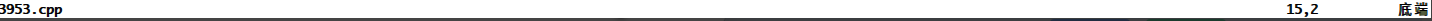
\includegraphics[width=0.7\textwidth]{docs/intro/images/airline1.png} 
\caption{airline1}
\end{figure}

\begin{figure}[htbp]
\centering
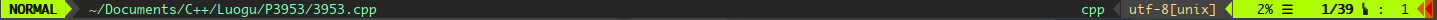
\includegraphics[width=0.7\textwidth]{docs/intro/images/airline2.png} 
\caption{airline2}
\end{figure}

然后,其实我们的 nerdtree 插件也是可以美化的,同时多安装一个小插件和一点配置即可达到美化效果,具体请移步配置篇食用。

\paragraph{启动界面}

这个其实可有可无,是一个能快捷键打开历史记录的一个插件 vimplus-startify,具体可以自己尝试。

\paragraph{小方便性插件}

commentary :快捷键 \texttt{gc} 注释选中行,\texttt{gcu} 撤销上次注释。

syntastic :\texttt{:w} 保存时提示语法错误,需配置中设置标错样式,如我的就会在行前显示 \texttt{>>}。

easymotion :快速跳转,我自己其实都不会用 233,需要可以查阅资料。

rainbow : 彩虹括号,使具有包含关系的括号显现出不同的颜色,增强多括号代码的可读性。

delimitMate : 括号补全功能。同时考试中可用配置实现部分功能,配置篇中会讲述。

vimcdoc :汉化 Vim 在线文档。

gundo :这个插件将能够显示你的文件修改树,就像 github 上一般能够回到历史版本,时光机啊 QwQ 。Vim 中\texttt{:GundoToggle}即可在左侧打开时光机。

vimim :这个的安装不在配置中,相当于 Vim 自带中文输入法,需在 \texttt{.vim} 中创建文件夹 plugin 并把 \href{https://www.vim.org/scripts/download_script.php?src_id=23122}{从这里} 下得的文件扔入此文件夹中即可。打开 Vim 并进入插入模式,按下 Ctrl + / 即可启用。但是使用的是云词库,若没网就会卡死。所以建议下载\href{https://github.com/vimim/vimim/raw/master/plugin/vimim.gbk.bsddb}{本地超大词库},也放入 plugin 文件夹中,与插件脚本同目录即可启用。

vim-instant-markdown :这个插件可就厉害了。Vim 用习惯了之后什么都想用 Vim 来做,比如想用 Vim 来写 Markdown 并实时预览怎么办?于是这个强大的插件就诞生了,当打开 Markdown 文件时会自动在浏览器中打开一个标签页,将能够实时预览你的 Vim 中的 markdown 内容。

一切插件的安装写法及快捷键及配置皆在配置篇中,请移步。

\subsubsection{配置篇}

\href{https://github.com/LuoshuiTianyi/Vim-for-OIWiki}{我的配置} Ps: 我的 .vimrc 时刻在改,所以这只是个副本……

结合我的配置讲一讲一些 Vim 中的小细节和快捷键以及一些…… 七里八里的东西?

Vim 的配置语法没那么麻烦,基本上就是 set 开启选项,call xxx() 调用函数,func 与 endfunc 定义函数,exec 执行命令,if 和 endif 描述以下条件表达式," 表示注释,source 表示应用啥的,语法和 Vim 命令行下一模一样,只是当你把配置文件写入,Vim 开启时会自动执行配置中的每一行语句。

\paragraph{基础设置}

我必须说我的配置里其实没有背景方面的设置,因为我黑背景加个透明化很舒服了…… 接下来我会挑重要的配置来讲,剩下的可以结合我的配置内的注释来看

首先使用各种插件容易与 vi 的模式产生冲突,所以我们要关闭 vi 的功能,那么就有了如下配置:

\begin{minted}{vim}
set nocompatible
\end{minted}

通过这个设置将关闭原有 vi 的功能以防冲突

随后,当你打开你的 cpp 文件时,你会发现及其之丑,因为没有了语法高亮,一切都是一个颜色了。那么配置中需加入如下两行

\begin{minted}{vim}
syntax enable
syntax on
\end{minted}

分别是开启高亮支持与开启语法高亮

然后是我们可爱的状态栏,\texttt{set laststatus=2} 这行配置将会使得状态栏总是显示,而状态栏所显示的信息在配置中是可以设置的。设置如下:

\begin{minted}{vim}
set statusline=\ %<%F[%1*%M%*%n%R%H]%=\ %y\ %0(%{&fileformat}\ [%{(&fenc==\"\"?&enc:&fenc).(&bomb?\",BOM\":\"\")}]\ %c:%l/%L%)
\end{minted}

这一行会使状态栏显示包括文件路径,模式,文件类型,文件编码,所在行数与列数,以及光标所在处是文件的百分之多少。加上 airline 插件,既美观又实用。

再然后,默认情况下换行符是不可被删除的,除非使用 \texttt{dd} 命令或者 \texttt{J} 命令才可做到。那么我们需要 \texttt{set backspace=indent,eol,start} 这行配置来解除这种限制。

显然还有一件事,那就是行号的问题。不管是评测文件写了多少行还是想要使用 \texttt{数字 + G} 的命令跳至指定行,没有行号的显示肯定是崩溃的。那么可以使用 \texttt{set number} 开启行号显示的功能。然后是 Vim 的自动折行功能,那就是当某一行超过了 Vim 窗口的边界,Vim 会怎么做呢?多出的部分会自动显示在下一行,而这种多出来的行前面是没有行号的,比较好辨认,这些行被称为屏幕行,而根据行号一一对应的便称作实际行。但是仅仅凭着看前面的行号来辨认某个折下来的行属于那个实际行的话,还是不够快。我们可以使用\texttt{set cursorline}来开启高亮显示当前行,而这个高亮也是可以设置的,我的配置里也有。

然后是我们在基础篇中提到过的,开启鼠标支持\texttt{set mouse=a},以及插件篇中提及的\texttt{set autochdir}与进阶篇中有的\texttt{set fillchars=vert:\textbackslash{} ,stl:\textbackslash{} ,stlnc:\textbackslash{}} 这三个配置,作用各有提及。

其他的往我配置里看啦 wwww。

那个 \texttt{zsh} 是一个 shell 的相关程序,有兴趣的可以查查,没兴趣的删掉吧 QwQ。

还有一件事,就是文件编码,设置如下:

\begin{minted}{vim}
set langmenu=zh_CN.UTF-8
set helplang=cn
set termencoding=utf-8
set encoding=utf8
set fileencodings=utf8,ucs-bom,gbk,cp936,gb2312,gb18030
\end{minted}

\paragraph{快捷键设置}

其实 Vim 普通模式下没有多少按键是 "自由身",那么用户该如何定制自己的快捷键呢?Vim 为此提供了 leader 键来服务。leader 键在配置中由自己定制,只需要短短一行

\begin{minted}{vim}
let mapleader = ""
\end{minted}

双引号之间就是你自己定义的 leader 键啦。

设置快捷键怎么写呢?

\begin{minted}{vim}
nnoremap 快捷键 指令
inoremap 快捷键 指令
\end{minted}

两行分别代表了在普通模式下和插入模式下的快捷键执行指令。当然指令不用想多了,没有什么语法,就是相当于在键盘上按你指令中写下的键而已……

首先我的个人快捷键需求其实不是很多,我的 leader 键是 ,但是处于一种坐冷板凳的状态,就更新插件的时候用一用,不过还是很方便的,我的设置是:

\begin{minted}{vim}
nnoremap <leader><leader>i :PluginInstall<CR>
\end{minted}

\texttt{<CR>}代表回车。设置之后只需要连续按 \texttt{}i 即可更新插件,很方便。

那么你有没有猜到如何利用配置写出括号补全的部分功能呢?没错,就是利用快捷键。将插入模式下的左扩号当做快捷键即可,指令就是\texttt{()}。如果补全后要使光标在括号里怎么办呢?如果仔细观察你就会发现每当退出插入模式,光标总是会向后跳一个字符,我们可以利用这一点,组合 \texttt{Esc + i} 不就变成了向前一个字符进行插入吗?总结下来配置如下:

\begin{minted}{vim}
inoremap (  ()<esc>i
inoremap [  []<esc>i
inoremap "  ""<esc>i
inoremap '  ''<esc>i
\end{minted}

当然我的配置里没有,而且我也不用括号补全插件,其实原因是因为我希望我的撤销树会更合理与好看。你会发现,括号补全为了使光标回到括号内,已经退出了一次插入模式,那么撤销命令的效果就不完整了。而且其实插入模式下使用方向键,也相当与推出插入模式移动又重新回到插入模式,也会使撤销树不完整 = =。所以你会发现进阶篇提到的,我的配置里那个丧心病狂的东西……

还记得进阶篇里的分屏吗?显然使用鼠标点击来选择活动窗口太慢,而移动命令前加个Ctrl+w也不习惯对不对,所以我的做法是用Ctrl+ 移动命令来映射前面的按键组合。

\begin{minted}{vim}
nnoremap <c-h> <c-w>h  
nnoremap <c-l> <c-w>l  
nnoremap <c-j> <c-w>j  
nnoremap <c-k> <c-w>k
\end{minted}

应该比原来的按法好记也好按…… 吧……

还记得自动折行吧,我们的\texttt{hjkl}命令其实都是在实际行之间移动,而折下来的屏幕行实在是没法子,只能用 \texttt{l} 键不断移过去。但实际上,\texttt{g + 移动命令} 便能够使你在屏幕行间移动,因为考虑到这种移动的常用,我选择将\texttt{g + 移动命令}与移动命令反过来映射。

\begin{minted}{vim}
noremap j gj
noremap gj j
noremap gk k
noremap k gk
\end{minted}

刚才也都说了,自由身的快捷键不多,\texttt{F1\textasciitilde{}F12} 就是方便而自由的快捷键。那用它们来干嘛呢?

F9一键编译

我想有了之前的编译命令,基础篇命令行模式中的介绍,你应该大概能有个思路了吧。作出的操作肯定如下:

\begin{minted}{vim}
:w   " 保存
:g++ xxx.cpp -o xxx " 编译
:./xxx " 运行
\end{minted}

那么如何实现呢?我倾向于写个函数:

\begin{minted}{vim}
nnoremap <F9> :call CompileRunGcc()<CR>
func! CompileRunGcc()
    exec "w" 
    exec '!g++ % -o %<'
    exec '!time ./%<'
    endfunc  
\end{minted}

第一行代表运行 \texttt{CompileRunGcc} 函数,第二行代表定义函数,三至五行代表函数运行内容,第六行代表函数结束。\texttt{exec} 表示执行命令,\texttt{\%} 表示当前文件名,\texttt{\%<} 表示当前文件名去掉后缀的名字。我想你应该是看得懂函数内容的。

不过如果你使用得多了,就会发现当按下 F9 的时候转到另一个屏即终端进行运行,但是每运行一次都会多一些信息。如此累积的话多来几次整个终端就满了,这时可以使用 bash 下的命令

\begin{minted}{shell}
clear
\end{minted}

来清屏,不过我倾向于也把它封装在一个快捷键内,按 F12 就会自动清屏了,个人觉得用着挺爽……

\begin{minted}{vim}
nnoremap <F12> :call Clss()<CR>
func! Clss()
    exec '!clear'
    endfunc
\end{minted}

还有,在 Vim 中执行外部命令纵使有 \texttt{:!} 的方法,其实还是不方便,要是能直接在 Vim 中再打开一个终端就好了,对吧。Vim 从 8.0 之后就增添了在内部分个屏来打开一个终端的功能,命令是 \texttt{:terminal}。我个人也将它设置成了快捷键,作为强迫症还是装在了函数中 = =。我想有了命令你应该自己会写了。

\begin{minted}{vim}
nnoremap <F8> :call Term()<CR>
func! Term()
    exec 'terminal'
    endfunc
\end{minted}

按F8就能在上面分出一个窗口打开终端了。

介于更各种 Vim 版本的压迫,Vim 作者也是奋发图强,Vim 8.1 又更新了调试程序,先用\texttt{packadd termdebug}开启此设置,然后在 Vim 中输入\texttt{:Termdebug + 编译出的程序名称}即可开始 GDB 的过程,具体详细操作可以参考\href{https://fzheng.me/2018/05/28/termdebug/}{这篇文章}。这个自然也被我封装函数了 >\textbackslash{}\_\&lt;。

\begin{minted}{vim}
packadd termdebug
nnoremap <F11> :call GDB()<CR>
func! GDB()
    exec 'Termdebug %<'
    endfunc       
\end{minted}

\paragraph{写代码好用的}

首先是 Tab 键,我们可以用 \texttt{set tabstop=} 来定义 Tab 的长度,一般当然是 4 个空格,在等于号后面填的数字是多少那么长度就是多少空格。

然后是写代码的时候,当多个括号嵌套时用肉眼显然不好看出对应的括号,那么我们可以用 \texttt{set showmatch} 开启高亮显示匹配括号。

有的时候打开 Vim 是不是经常会提示有什么 swap 文件是否确认啥的,那个是临时缓存文件,挺烦的,我们可以使用 \texttt{set nobackup} 与 \texttt{set noswapfilei} 来禁止其生成,这样就方便舒爽多了(还是开着吧)。

最后嘛,大多数时候调试代码都会用 \texttt{freopen} 来输入输出,再利用分屏操作来打开 \texttt{.in} \texttt{.out} 文件,就可以实时看到结果。不过每次运行程序之后你都会发现因为 \texttt{.out} 文件的修改而会弹出一个确认选项是否重新加载文件,这个也是很不爽的,我们可以开启 \texttt{set autoread} 选项以自动加载改动的文件。

\paragraph{关于插件}

插件篇中说到了强大的插件管理器 Vundle,那么在配置中该如何写呢?框架如下:

\begin{minted}{vim}
set rtp+=~/.vim/bundle/Vundle.vim
call vundle#begin('~/.vim/自己创建的用来放插件文件的文件夹')

call vundle#end()
\end{minted}

在两块之间来写需要安装的插件,格式如下:

\begin{minted}{vim}
Plugin '作者 Github 上的名字/Github 上的插件仓库名'
\end{minted}

写完保存后进入 Vim,使用 \texttt{:PluginInstall} 即可自动开始安装。

我的插件列表:

\begin{minted}{vim}
set rtp+=~/.vim/bundle/Vundle.vim
call vundle#begin('~/.vim/plugged')

Plugin 'VundleVim/Vundle.vim'                    " 使用Vundle的必须配置
Plugin 'chxuan/vimplus-startify'                 " 启动界面
Plugin 'scrooloose/nerdtree'                     " 目录树
Plugin 'tiagofumo/vim-nerdtree-syntax-highlight' " 目录树美化
Plugin 'vim-airline/vim-airline'                 " 状态栏美化
Plugin 'vim-airline/vim-airline-themes'          " 状态栏美化主题
Plugin 'tpope/vim-commentary'                    " 快速注释
Plugin 'scrooloose/syntastic'                    " 语法错误提示
Plugin 'Lokaltog/vim-easymotion'                 " 快速跳转
Plugin 'luochen1990/rainbow'                     " 彩虹括号
"Plugin 'Raimondi/delimitMate'                   " 括号补全
Plugin 'yianwillis/vimcdoc'                      " HELP文档中文
Plugin 'sjl/gundo.vim'                           " 撤销树
Plugin 'suan/vim-instant-markdown'               " markdown 实时预览

call vundle#end()
\end{minted}

关于插件其实也有相关配置,但是都写在一起将会使得 \texttt{.vimrc} 十分臃肿,我们可以额外写在别的文件里,一般文件应该保存在 \texttt{home} 下,然后在配置中写下 \texttt{source \$HOME / 文件路径} 即可。我的 nerdtree, syntastic 和 airline 都额外写了别的文件。

同时我的配置里关于插件的快捷键如下:

\begin{minted}{vim}
F10 :启动 nerdtree 侧边工程目录树
F7  :启动 Gundo 时光机
\end{minted}

\subsubsection{关于高效编辑的建议}

为什么 Emacs 和 Vim 这些编辑器效率高?  

很重要的一点在于这些编辑器可以让你切掉你的右半部分的键盘而让你的双手始终处于主键盘区域, 并且让你的双手保持合作, 而不会出现一只手不停的按而另一只手摊在键盘上。  

所以, 如果你想用好 Vim(或者其他高级编辑器), 不要去按方向键, 不要去碰鼠标, 你甚至可以强迫自己:  

\begin{minted}{vim}
" 使方向键失效
inoremap <UP> a<Bs>
inoremap <DOWN> a<Bs>
inoremap <LEFT> a<Bs>
inoremap <RIGHT> a<Bs>
\end{minted}

但也许这还不够, 你还可以进一步缩小你双手需要控制的区域。  

\begin{itemize}
\item Esc 键在 Vim 中使用频繁, 虽然有 ctrl+\textbackslash{}[ 来代替它, 但这仍然不够。  
事实上还用一种高效却鲜为人知的办法: \textbf{用 alt}。  
在 TUI(终端) 中任何模式 alt + 任何按键完全等效于 Esc + 该按键。  
例如你要退出插入模式向上移动, 普通做法是 Esc+k, 但 alt+k 有同样的效果并且十分高效。  
\item Backspace (删除键) 使用十分频繁, 但它处在主键盘的角落, 你不得不挪开手或是伸长小拇指。  
但在 Vim (甚至终端) 里, 你可以用 ctrl+h 来彻底代替 Backspace。  
\item 回车键使用同样频繁, 但同样不挪一挪手就得伸长小拇指。  
幸运的是在 Vim 和终端中, ctrl+m 完全等效与回车。  
\item 在绝大多数的情况下, 不要去按右边的 ctrl, shift, 用左边的代替。  
\item 最好不用 F1 到 F12, 如果要映射, 用 Leader 开头的自定义快捷键。  
\end{itemize}

\subsection{Visual Studio Code - 微软家的编辑器}

\subsubsection{简介}

Visual Studio Code (以下简称 VS Code) 是一个免费、开源、跨平台的由微软开发的程序编辑器。它是用 Typescript 编写的,并且采用 Electron 架构。官网是 \url{https://code.visualstudio.com/} 。它带有对 JavaScript、TypeScript 和 Node.js 的内置支持,并为其他语言(如 C++、Cype、Java、Python、PHP、GO)提供了丰富的扩展生态系统。

对比 Sublime 和 Atom,它有以下优点:

\begin{itemize}
\item 快速
\item 美观
\item 社区生态好
\item ……
\end{itemize}

  \section{WSL (Windows 10)}
  
\begin{figure}[htbp]
\centering
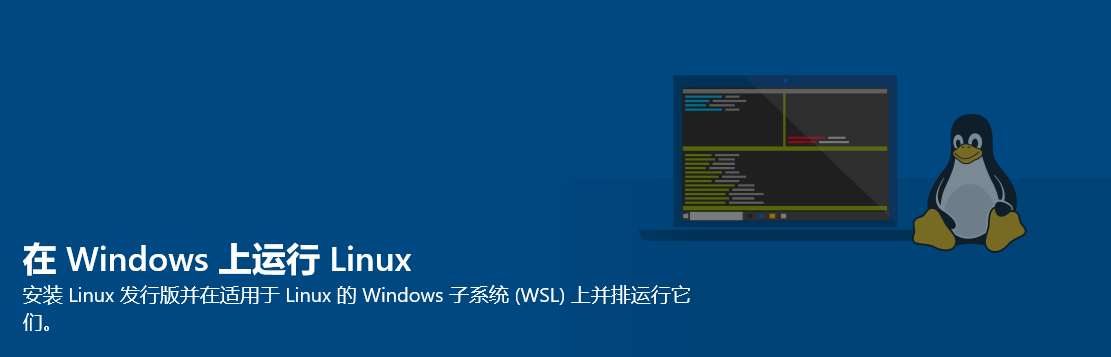
\includegraphics[width=0.7\textwidth]{docs/intro/images/WSL1.png} 
\caption{头图}
\end{figure}

\hr

\subsection{0x01 引言}

众所周知,尽管现在大部分学校的竞赛练习环境都是构建 XP 等 Windows 系操作系统,但是在 NOI 系列赛中,早已用上了 NOI Linux 这个 Ubuntu 操作系统的阉割版。  

\begin{figure}[htbp]
\centering
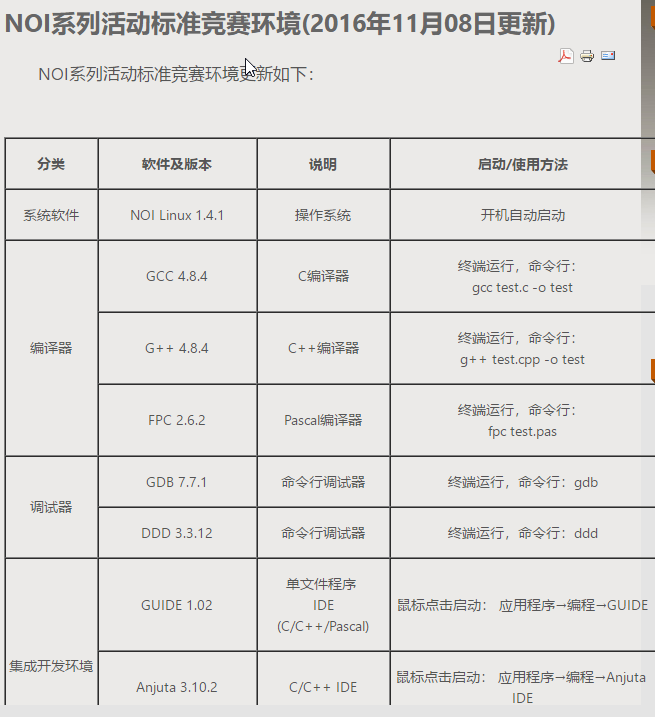
\includegraphics[width=0.7\textwidth]{docs/intro/images/WSL2.png} 
\caption{NOI 竞赛的环境要求}
\end{figure}           



或许大家对自己 Windows 环境下的 Dev-C++ 等都已熟识,但是当场景突然切换到 Linux 的时候,你会不会不知所措?

\begin{QUOTE}{}{}
「想用 Ctrl+C 复制,结果退出了程序」  



「平时 AC 的程序模板到了 Linux 上就 WA」……
\end{QUOTE}

\begin{figure}[htbp]
\centering
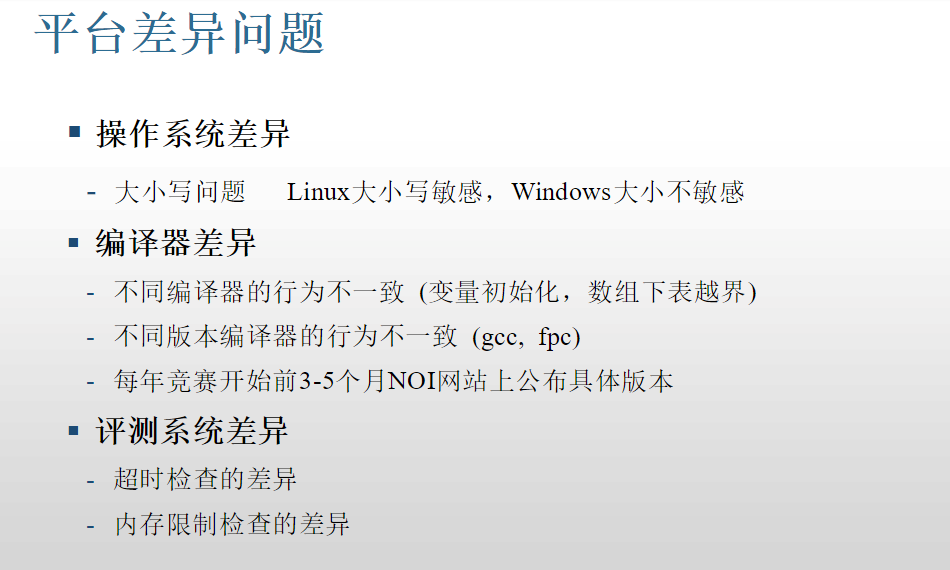
\includegraphics[width=0.7\textwidth]{docs/intro/images/WSL3.png} 
\caption{平台差异(转自百度文库”NOIP 标准评测系统及相关问题 “)}
\end{figure}



虽然在 NOI 的官网已经放出了 NOI Linux 的 ISO 镜像,但是如果跑虚拟机的话,配置也相当麻烦,包括激活 VMware,用 VMware 装系统开虚拟机等步骤,且 NOI Linux 默认自带图形界面,两个系统一起运行是低配党的噩梦。

Windows 10 作为微软的新一代操作系统,紧跟时代潮流,在一周年更新时推出了 Linux 子系统(WSL),可以供装不起 VMware 等虚拟机的同学食用。  

缺点是没有 NOI 评测用的 \textbf{Arbiter},但是在各大 OJ 背书的情况下谁在乎呢……

\begin{NOTE}{补充资料:何为 Linux 子系统(WSL)?(via 百度百科)}{}
 Windows Subsystem for Linux(简称 WSL)是一个为在 Windows 10 上能够原生运行 Linux 二进制可执行文件(ELF 格式)的兼容层。它是由微软与 Canonical 公司合作开发,目标是使纯正的 Ubuntu, OpenSUSE, Kali Linux 和 Debian 映像能下载和解压到用户的本地计算机,并且映像内的工具和实用工具能在此子系统上原生运行。  
 WSL 提供了一个微软开发的 Linux 兼容内核接口(不包含 Linux 代码),来自 Linux 的用户模式二进制文件在其上运行。  
 此子系统起源于命运多舛的 Astoria 项目,其目的是允许 Android 应用运行在 Windows 10 Mobile 上。此功能组件从 Windows 10 Insider Preview build 14316 开始可用。

\end{NOTE}


\hr

\subsection{0x02 准备}

首先,你需要一个最新的 Windows 10 操作系统,这点不必多说。  

其次,你需要配置一下开发人员模式环境。

\begin{enumerate}
\item 设置 -> 更新与安全 -> 开发人员模式框选 -> 是
\begin{figure}[htbp]
\centering
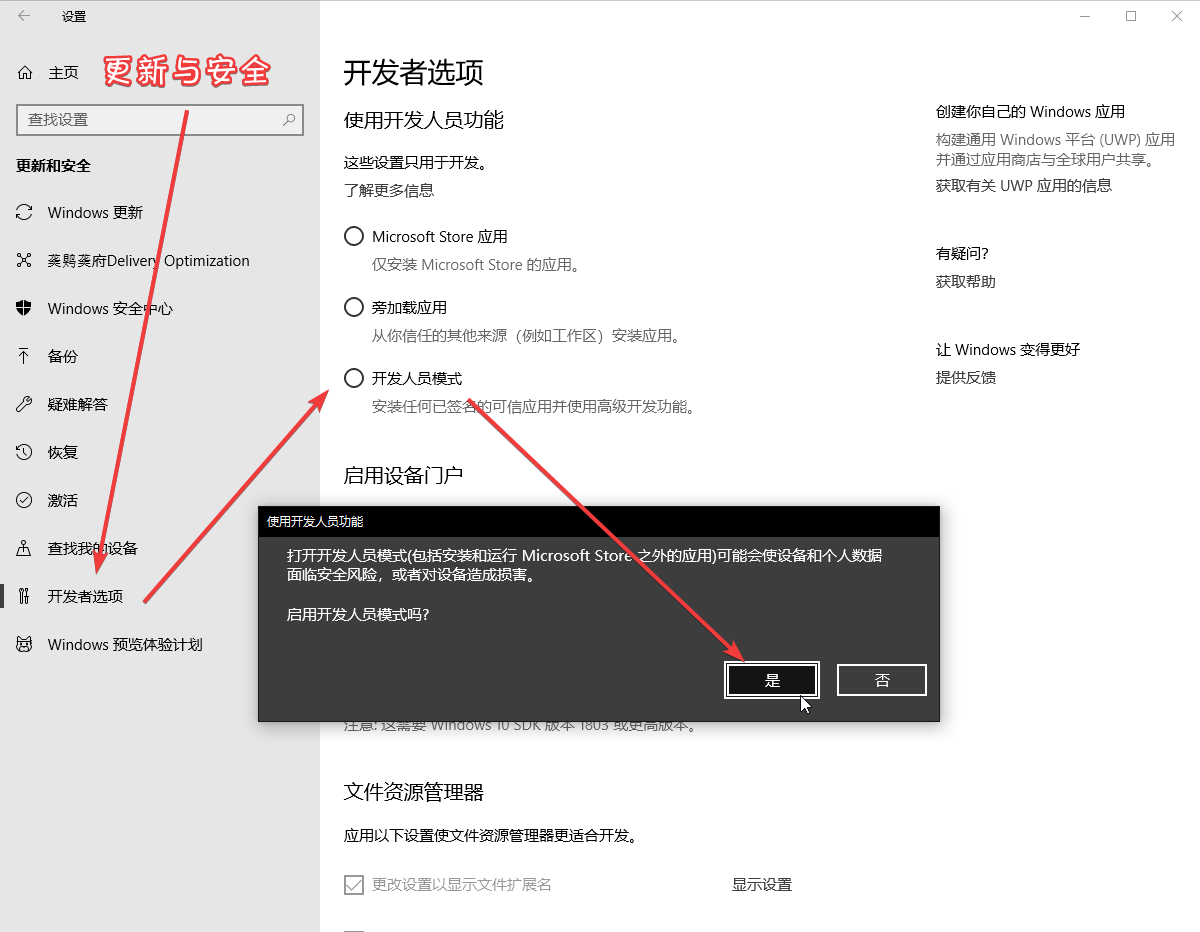
\includegraphics[width=0.7\textwidth]{docs/intro/images/WSL4.png} 
\caption{来,跟着箭头走}
\end{figure}     
\end{enumerate}



\textbf{Linux 区分大小写!}

\begin{figure}[htbp]
\centering
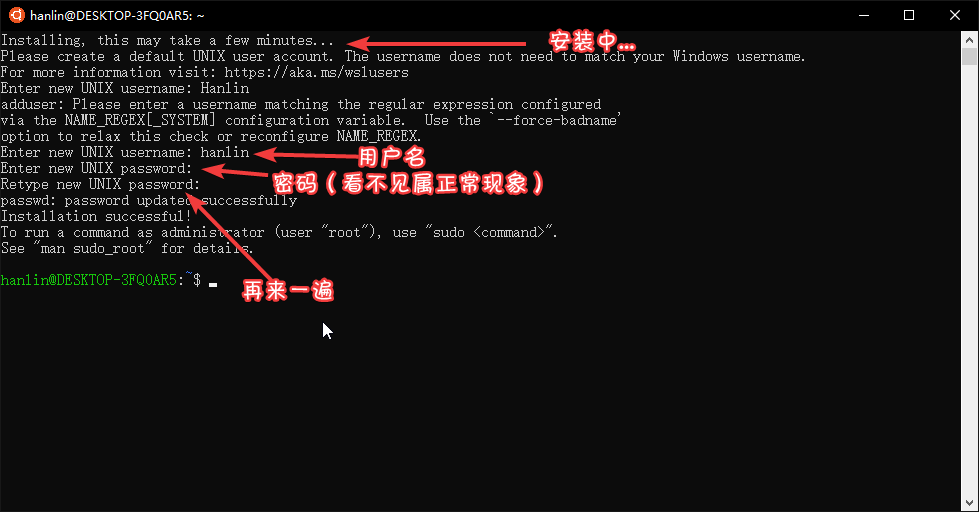
\includegraphics[width=0.7\textwidth]{docs/intro/images/WSL6.png} 

\end{figure}

 这样之后,一个纯净的 Ubuntu 系统安装完成了!

\subsection{0x04 基础配置}

 \textbf{ 以下命令均可直接右键复制粘贴进窗口哦!}

\begin{figure}[htbp]
\centering
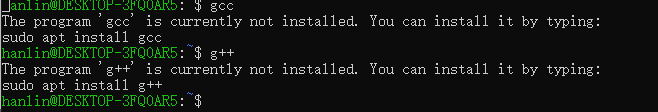
\includegraphics[width=0.7\textwidth]{docs/intro/images/WSL7.png} 

\end{figure}

 正如图片所示,这个系统纯净到连个编译器都没有,所以这一节来看看基础的环境配置。

\subsubsection{更换为国内软件源}

Ubuntu 默认的软件源在国外,我们可以换为国内的加快速度,如 \href{https://mirrors.tuna.tsinghua.edu.cn/help/ubuntu/}{清华 TUNA 的软件源}。  

可以访问 \href{https://mirrors.tuna.tsinghua.edu.cn/help/ubuntu/}{TUNA 的页面} 来获得国内源的信息。

\begin{WARNING}{}{}
 请在页面中寻找与自己系统版本相配的源(可使用 \texttt{sudo lsb\_release -a} 查看,具体详见 \texttt{0x03} )  
 除非你知道你在做什么,否则不要使用与自己的系统版本不匹配的源!     

\end{WARNING}


使用的命令

\begin{minted}{bash}
sudo cp /etc/apt/sources.list /etc/apt/sources.list.bak
sudo vim /etc/apt/sources.list
# (按 i 之后将上文的源右键粘贴进去,编辑完后按 Esc,再输入 :wq 和回车)
sudo apt update
sudo apt upgrade -y
\end{minted}

\begin{figure}[htbp]
\centering
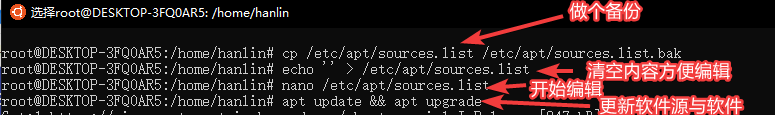
\includegraphics[width=0.7\textwidth]{docs/intro/images/WSL9.png} 

\end{figure}

\subsubsection{安装中文环境}

\begin{minted}{bash}
sudo apt install  language-pack-zh-han* -y
sudo locale-gen zh_CN.GB18030 && sudo locale-gen zh_CN.GB2312 && sudo locale-gen zh_CN.UTF8
# 中文字体,别忘了同意 EULA
sudo apt install fontconfig -y
sudo apt install ttf-mscorefonts-installer -y
# 下面的再执行一遍以防万一
sudo apt install -y --force-yes --no-install-recommends fonts-wqy-microhei
sudo apt install -y --force-yes --no-install-recommends ttf-wqy-zenhei
sudo dpkg-reconfigure locales
\end{minted}

使用 \texttt{sudo dpkg-reconfigure locales} 进入菜单,按空格选择带 \texttt{zh\_CN} 的选项,选完后回车,下一个菜单中选 \texttt{zh\_CN.UTF-8} 打回车。

\begin{figure}[htbp]
\centering
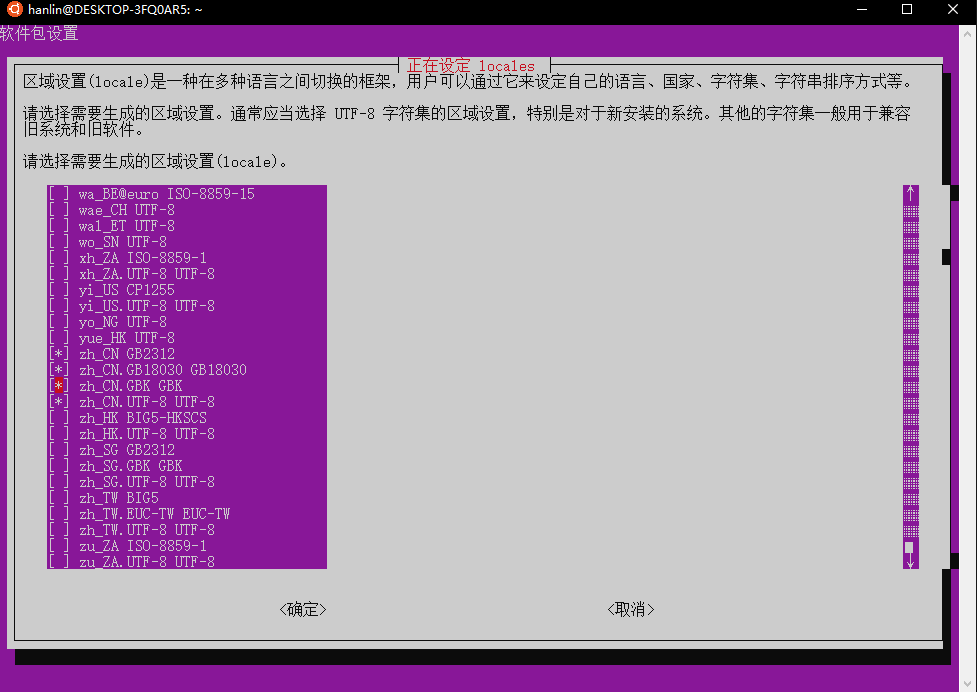
\includegraphics[width=0.7\textwidth]{docs/intro/images/WSL10.png} 

\end{figure}

\begin{figure}[htbp]
\centering
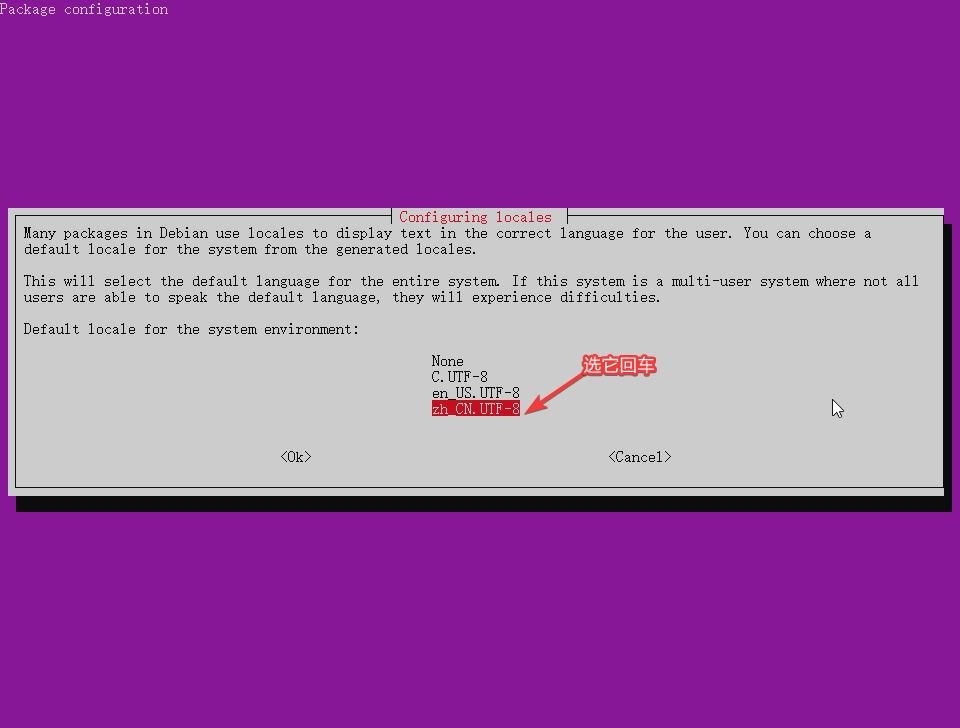
\includegraphics[width=0.7\textwidth]{docs/intro/images/WSL11.png} 

\end{figure}

 之后关上 Ubuntu 重开一遍登录,是不是变中文了?

再依次输入下列命令,把 \texttt{man} 帮助页替换为中文:\href{https://blog.csdn.net/qq_14989227/article/details/72954523}{via}

\begin{minted}{bash}
sudo apt install manpages-zh
sudo vi /etc/manpath.config
:1,$s#/usr/share/man#/usr/share/man/zh_CN#g
:wq
\end{minted}

 可以用 \texttt{man help} 测试下。

\subsubsection{安装编译环境}

\begin{minted}{bash}
sudo apt install build-essential vim ddd gdb fpc emacs gedit anjuta lazarus -y
wget http://download.noi.cn/T/noi/GUIDE-1.0.2-ubuntu.tar
tar -xvf GUIDE-1.0.2-ubuntu.tar
cd GUIDE-1.0.2-ubuntu
chmod +x install.sh && ./install.sh
\end{minted}

这是基础的 + NOI 官方要求环境,如有需要可以用 \texttt{apt install 程序名} 来安装别的。

若想安装其他版本可以参考下 \href{https://www.cnblogs.com/EasonJim/p/7144017.html}{这个}

来个程序玩玩:

\begin{minted}{bash}
$ vim cpuid.cpp
$ g++ -Wall cpuid.cpp -o cpuid
$ ./cpuid
AMD Ryzen 5 1400 Quad-Core Processor
\end{minted}

\textbf{Tips:Linux 环境下可执行文件可不带扩展名,实现方式看上方命令行 }

\subsection{0x05 进阶操作}

\subsubsection{安装图形环境,并使用远程桌面连接}

推荐图形环境用 xfce4,不臃肿。

\begin{minted}{bash}
sudo apt install xfce4 tightvncserver -y
# 或使用 sudo apt install xubuntu-desktop -y
# xubuntu 安装的软件多,基础环境可用第一种
\end{minted}

图形环境是个大头,因此要多等会,静静等待下载解包。

下面配置 xrdp:

\begin{minted}{bash}
sudo apt install xrdp -y
echo "xfce4-session" >~/.xsession
sudo service xrdp restart
\end{minted}

 为了防止和你计算机本来带的远程桌面冲突,最好换一下端口。

\begin{figure}[htbp]
\centering
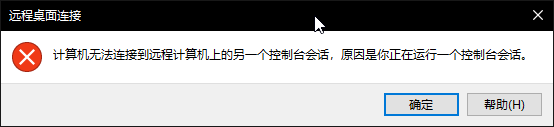
\includegraphics[width=0.7\textwidth]{docs/intro/images/WSL12.png} 

\end{figure}



\begin{enumerate}
\item \href{https://wenku.baidu.com/view/8246d96cdd36a32d72758143.html}{NOIP 标准评测系统及相关问题, smart0326, 2014-05-19, 百度文库}         
\item \href{https://baike.baidu.com/item/wsl/20359185}{WSL, 百度百科}        
\item \href{https://blogs.windows.com/buildingapps/2016/03/30/run-bash-on-ubuntu-on-windows/#cie8WdR3uSjgR5Ru.97}{Run Bash on Ubuntu on Windows, Mike Harsh, 2016-05-30, Windows Blog}         
\item \href{https://docs.microsoft.com/zh-cn/windows/wsl/about}{Windows Subsystem for Linux Documentation, MSDN}      
\item \href{http://www.noi.cn/2016-11-08-03-42-01}{NOI 系列活动标准竞赛环境, 2016-11-08, NOI 官网}      
\item \href{https://www.microsoft.com/zh-cn/p/ubuntu/9nblggh4msv6}{购买 Ubuntu, Microsoft Store}      
\item \href{https://mirrors.tuna.tsinghua.edu.cn/help/ubuntu/}{Ubuntu 镜像使用帮助, 清华 TUNA}      
\item \href{https://blog.csdn.net/qq_14989227/article/details/72954523}{Ubuntu 的 man 命令帮助如何设置中文版, Frank 看庐山, 2017-06-09}      
\item \href{https://sourceforge.net/projects/xming/}{Xming X Server for Windows, SourceForge}       
\item \href{https://zh.wikipedia.org/wiki/Sudo}{Sudo, Wikipedia}       
\end{enumerate}

\subsection{0x09 延伸内容}

\href{https://spencerwoo.com/dowww/}{Dev on Windows with WSL(在 Windows 上用 WSL 优雅开发)}

\subsubsection{后记}

本文最初发布于 \href{https://www.luogu.org/discuss/show/48491}{洛谷日报 \textbackslash{}\#6},现由原作者搬运至此,有删改。      

  \section{Special Judge}
  
一道题如果有多组解,我们就需要一个程序来判断答案合法性,这便是 Special Judge (spj),又常被称作 checker,下面介绍部分评测工具 /OJ 的 spj 编写方法。

\begin{WARNING}{}{}
spj 还应当判断文件尾是否有多余内容,及输出格式是否正确(如题目要求数字间用一个空格隔开,而选手却使用了换行)。但是,目前前者只有 Testlib 可以方便地做到这一点,而后者几乎无人去特意进行这种判断。

浮点数时应注意 nan,不合理的判断方式会导致输出 nan 即可 AC。

\end{WARNING}


以下均使用 C++,以 “要求标准答案与选手答案差值小于 1e-3,文件名为 num” 为例。

\subsection{Testlib}

\href{https://codeforces.com/testlib}{Testlib} 是一个强大的算法竞赛题目辅助系统,只需要在程序中引入 \href{https://github.com/MikeMirzayanov/testlib/blob/master/testlib.h}{testlib.h} 头文件即可使用。用法详见  Testlib  页面。

使用 Testlib 编写 spj 的好处为我们不再需要判断文件尾的多余内容,其会帮助我们自动判断,也无需担忧 nan。

必须使用 Testlib 做 spj 的 评测工具 /OJ:Codeforces、洛谷、UOJ 等

可以使用 Testlib 做 spj 的 评测工具 /OJ:LibreOJ(SYZOJ 2)、Lemon 等

SYZOJ 2 所需的修改版 Testlib 可以在\href{https://pastebin.com/3GANXMG7}{这里}获取到,感谢 \href{https://loj.ac/article/124}{cyand1317}。

Lemon 所需的修改版 Testlib 可以在\href{https://paste.ubuntu.com/p/JsTspHHnmB/}{这里}获取到,感谢 matthew99。注意此版本 Testlib 注册 checker 应使用 \texttt{registerLemonChecker()} 而非 \texttt{registerTestlibCmd()}。

其他评测工具 /OJ 大部分需要按照其 spj 编写格式修改 Testlib。

\begin{cppcode}
#include <testlib.h>
#include <cmath>
int main(int argc, char *argv[]) {
  /*
   * inf:输入
   * ouf:选手输出
   * ans:标准输出
   */
  registerTestlibCmd(argc, argv);
  double pans = ouf.readDouble(), jans = ans.readDouble();
  if (abs(pans - jans) < 1e-3)
    quitf(_ok, "Good job");
  else
    quitf(_wa, "Too big or too small, expected %f, found %f", jans, pans);
}
\end{cppcode}

\subsection{Lemon}

\textbf{Lemon 有现成的修改版 Testlib,建议使用 Testlib,见  Testlib }

\begin{cppcode}
#include <cmath>
#include <cstdio>
int main(int argc, char* argv[]) {
  /*
   * argv[1]:输入
   * argv[2]:选手输出
   * argv[3]:标准输出
   * argv[4]:单个测试点分值
   * argv[5]:输出最终得分
   * argv[6]:输出错误报告
   */
  FILE* fin = fopen(argv[1], "r");
  FILE* fout = fopen(argv[2], "r");
  FILE* fstd = fopen(argv[3], "r");
  FILE* fscore = fopen(argv[5], "w");
  FILE* freport = fopen(argv[6], "w");
  double pans, jans;
  fscanf(fout, "%lf", &pans);
  fscanf(fstd, "%lf", &jans);
  if (abs(pans - jans) < 1e-3) {
    fprintf(fscore, "%s", argv[4]);
    fprintf(freport, "Good job");
  } else {
    fprintf(fscore, "%d", 0);
    fprintf(freport, "Too big or too small, expected %f, found %f", jans, pans);
  }
}
\end{cppcode}

\subsection{Cena}

\begin{cppcode}
#include <cmath>
#include <cstdio>
int main(int argc, char* argv[]) {
  /*
   * FILENAME.in:输入
   * FILENAME.out:选手输出
   * argv[2]:标准输出
   * argv[1]:单个测试点分值
   * score.log:输出最终得分
   * report.log:输出错误报告
   */
  FILE* fin = fopen("num.in", "r");
  FILE* fout = fopen("num.out", "r");
  FILE* fstd = fopen(argv[2], "r");
  FILE* fscore = fopen("score.log", "w");
  FILE* freport = fopen("report.log", "w");
  double pans, jans;
  fscanf(fout, "%lf", &pans);
  fscanf(fstd, "%lf", &jans);
  if (abs(pans - jans) < 1e-3) {
    fprintf(fscore, "%s", argv[1]);
    fprintf(freport, "Good job");
  } else {
    fprintf(fscore, "%d", 0);
    fprintf(freport, "Too big or too small, expected %f, found %f", jans, pans);
  }
}
\end{cppcode}

\subsection{CCR}

\begin{cppcode}
#include <cmath>
#include <cstdio>
int main(int argc, char* argv[]) {
  /*
   * stdin:输入
   * argv[3]:选手输出
   * argv[2]:标准输出
   * stdout:L1:输出最终得分比率
   * stdout:L2:输出错误报告
   */
  FILE* fout = fopen(argv[3], "r");
  FILE* fstd = fopen(argv[2], "r");
  double pans, jans;
  fscanf(fout, "%lf", &pans);
  fscanf(fstd, "%lf", &jans);
  if (abs(pans - jans) < 1e-3) {
    printf("%d\n", 1);
    printf("Good job");
  } else {
    printf("%d\n", 0);
    printf("Too big or too small, expected %f, found %f", jans, pans);
  }
}
\end{cppcode}

\subsection{Arbiter}

\subsection{HUSTOJ}

\begin{cppcode}
#include <cmath>
#include <cstdio>
#define AC 0
#define WA 1
int main(int argc, char* argv[]) {
  /*
   * argv[1]:输入
   * argv[3]:选手输出
   * argv[2]:标准输出
   * exit code:返回判断结果
   */
  FILE* fout = fopen(argv[3], "r");
  FILE* fstd = fopen(argv[2], "r");
  double pans, jans;
  fscanf(fout, "%lf", &pans);
  fscanf(fstd, "%lf", &jans);
  if (abs(pans - jans) < 1e-3)
    return AC;
  else
    return WA;
}
\end{cppcode}

\subsection{QDUOJ}

QDUOJ 就麻烦一点,因为它的带 spj 的题目没有标准输出,只能把 std 写进 spj 跑出标准输出再判断。

\begin{cppcode}
#include <cmath>
#include <cstdio>
#define AC 0
#define WA 1
#define ERROR -1
double solve(...) {
  // std
}
int main(int argc, char* argv[]) {
  /*
   * argv[1]:输入
   * argv[2]:选手输出
   * exit code:返回判断结果
   */
  FILE* fin = fopen(argv[1], "r");
  FILE* fout = fopen(argv[2], "r");
  //读入
  double pans, jans;
  fscanf(fout, "%lf", &pans);
  jans = solve(...);
  if (abs(pans - jans) < 1e-3)
    return AC;
  else
    return WA;
}
\end{cppcode}

\subsection{LibreOJ(SYZOJ 2)}

\textbf{LibreOJ(SYZOJ 2) 有现成的修改版 Testlib,建议使用 Testlib,见  Testlib }

\begin{cppcode}
#include <cmath>
#include <cstdio>
int main(int argc, char* argv[]) {
  /*
   * in:输入
   * user_out:选手输出
   * answer:标准输出
   * code:选手代码
   * stdout:输出最终得分
   * stderr:输出错误报告
   */
  FILE* fin = fopen("in", "r");
  FILE* fout = fopen("user_out", "r");
  FILE* fstd = fopen("answer", "r");
  FILE* fcode = fopen("code", "r");
  double pans, jans;
  fscanf(fout, "%lf", &pans);
  fscanf(fstd, "%lf", &jans);
  if (abs(pans - jans) < 1e-3) {
    printf("%d", 100);
    fprintf(stderr, "Good job");
  } else {
    printf("%d", 0);
    fprintf(stderr, "Too big or too small, expected %f, found %f", jans, pans);
  }
}
\end{cppcode}

  \section{Testlib}
  



\section{关于本项目}

Q:你们是为什么想要做这个 Wiki 的呢?

A:不知道你在学 \textbf{OI} 的时候,面对庞大的知识体系,有没有感到过迷茫无助的时候?\textbf{OI Wiki} 想要做的事情可能类似于 “让更多竞赛资源不充裕的同学能方便地接触到训练资源”。当然这么表述也不完全,做 Wiki 的动机可能也很纯粹,只是简单地想要对 \textbf{OI} 的发展做出一点点微小的贡献吧。XD

Q:我很感兴趣,怎么参与呢?

A:\textbf{OI Wiki} 现在托管在 \href{https://github.com/24OI/OI-wiki}{GitHub} 上,你可以直接访问这个 \href{https://github.com/24OI/OI-wiki}{repo} 来查看最新进展。参与的途径包括在 \href{https://github.com/24OI/OI-wiki}{GitHub} 上面开 Issue、Pull Request,或者在交流群中分享你的想法、直接向管理员投稿。目前,我们使用的框架是 \href{https://mkdocs.readthedocs.io}{mkdocs},支持 Markdown 格式(也支持插入数学公式)。

Q:可是我比较弱…… 不知道我能做点什么?

A:一切源于热爱。你可以协助其他人审核修改稿件,帮助我们宣传 \textbf{OI Wiki} ,为社区营造良好学习交流氛围!

Q:现在主要是谁在做这件事啊?感觉这是个大坑,真的能做好吗?

A:最开始主要是一些退役老年选手在做这件事,后来遇到了很多志同道合的小伙伴:有现役选手,退役玩家,也有从未参加过 \textbf{OI} 的朋友。目前,这个项目主要是由 \textbf{OI Wiki} Team 来维护。(下面是一张合影)



当然,这个项目只靠我们的力量是很难做得十全十美的,我们诚挚地邀请你一起来完善 \textbf{OI Wiki}。

Q:听说过 nocow 吧,\textbf{OI Wiki} 怎么保证我们添加的内容不会像 nocow 那样突然间就不见了呢?

A:我们把内容托管在 \href{https://github.com/24OI/OI-wiki}{GitHub} 上面,即使我们的服务器翻车了,内容也不会丢失。另外,我们也会定期备份大家的心血,即使有一天 \href{https://github.com/24OI/OI-wiki}{GitHub} 倒闭了(?),我们的内容也不会丢失。

Q:\textbf{OI Wiki} 好像现在大部分内容都是空的啊?

A:是的,目前进度只完成了 57\% (重新统计于 2018.9.13),还远远称不上是一个合格的 Wiki。在过去的几个月里,主要添加的内容也比较基础。所以在这里进行征稿和招募,希望可以遇到有同样想法的朋友,我们一起把 \textbf{OI Wiki} 完善起来。

Q:为什么不直接去写 \href{https://zh.wikipedia.org/}{中文维基} 呢?

A:因为我们希望可以真正帮到更多的选手或者对这些内容感兴趣的人,由于众所周知的原因,中文维基上的内容并不是无门槛就可以获取到的。

\hr

感谢你看到了最后,我们现在急需的,就是你的帮助。

\textbf{OI Wiki} Team

2018.8

\chapter{基础部分}

\section{基础部分简介}

介绍一些基础知识,为之后的进阶内容做铺垫。

\begin{todolist}
\item[\done] 枚举
\item[\done] 模拟
\item[\done] 分治
\item[\done] 贪心
\item[\done] 排序
\item[\done] 表达式求值
\item[\done] 二分
\item[\done] 构造
\end{todolist}

\section{枚举}

枚举是基于已有知识来猜测答案的一种问题求解策略。

\begin{NOTE}{例题}{}
求小于 N 的最大素数
\end{NOTE}


找不到合适的一个数学公式来直接计算答案,不妨依次尝试一个数是否是答案。

如果我们从大到小枚举小于 $N$ 的数,那么原问题转化为如何判断一个数是不是素数。

注意到素数的性质要求不能被 $1$ 和它本身之外的数整除,可以直接用于判断。

枚举的思想是不断地猜测,从可能的集合中一一尝试,然后再判断题目的条件是否成立。

\subsection{给出解空间}

建立简洁的数学模型。

枚举的时候要想清楚可能的情况是什么,要枚举哪些要素?

\subsection{减少枚举的空间}

枚举的范围是什么?是所有的内容都需要枚举吗?

在用枚举法解决问题的时候,一定要想清楚这两件事,否则会带来不必要的时间开销。

\begin{NOTE}{例题}{}
一个数组中的数互不相同,求其中和为 $0$ 的数对的个数

\end{NOTE}


枚举两个数的代码很容易就可以写出来。

\begin{cppcode}
for (int i = 0; i < n; ++i)
  for (int j = 0; j < n; ++j)
    if (a[i] + a[j] == 0) ++ans;
\end{cppcode}

我们来看看枚举的范围如何优化。原问题的答案由两部分构成,两个数相等的情况和不相等的情况。相等的情况只需要枚举每一个数判断一下是否合法。至于不相等的情况,由于题中没要求数对是有序的,答案就是有序的情况的两倍(考虑如果 \texttt{(a, b)} 是答案,那么 \texttt{(b, a)} 也是答案)。我们对于这种情况只需统计人为要求有顺序之后的答案,最后再乘上 $2$ 就好了。

我们不妨要求第一个数要出现在靠前的位置。代码如下:

\begin{cppcode}
for (int i = 0; i < n; ++i)
  for (int j = 0; j < i; ++j)
    if (a[i] + a[j] == 0) ++ans;
\end{cppcode}

不难发现这里已经减少了 $j$ 的枚举范围,减少了这段代码的时间开销。

然而这并不是最优的结果。

两个数是否都一定要枚举出来呢?这里我们发现枚举其中一个数之后,题目的条件已经帮我们确定了其他的要素(另一个数),如果能找到一种方法直接判断题目要求的那个数是否存在,就可以省掉枚举后一个数的时间了。

\begin{cppcode}
// 要求 a 数组中的数的绝对值都小于 MAXN
bool met[MAXN * 2];
// 初始化 met 数组为 0;
memset(met, 0, sizeof(met));
for (int i = 0; i < n; ++i) {
  if (met[a[i] + MAXN]) ++ans;
  // 为了避免负数下标
  met[a[i] + MAXN] = 1;
}
\end{cppcode}

\subsection{选择合适的枚举顺序}

比如第一个例题中要求的是最大的符合条件的素数。自然是从大到小枚举比较合适。

\section{模拟}

模拟。顾名思义,就是用计算机来模拟题目中要求的操作,比如 NOIP 2014 的 \href{https://loj.ac/problem/2498}{生活大爆炸版石头剪刀布},只需要按照题面的意思来写就可以了。

当然,模拟一般也不是很好写,参见经典题目 \href{http://bailian.openjudge.cn/practice/3750/}{魔兽世界} 和 \href{https://www.lydsy.com/JudgeOnline/problem.php?id=1972}{猪国杀}。

模拟题目通常具有码量大、操作多、思路繁复的特点。并且由于它码量大,会导致很难查错,如果是在考试上是相当浪费时间的。

所以写模拟题,遵循以下的建议有可能会帮助你减少浪费时间

\begin{enumerate}
\item 在动手写代码之前,在草纸上尽可能的写好要实现的流程
\item 在代码中,尽量把每个部分模块化、写成函数、结构体或类
\item 对于一些可能重复用到的概念,可以统一转化,方便处理 : 如,某题给你 "YY-MM-DD 时: 分" 把它扔到一个函数处理成秒,会减少概念混淆
\item 调试时分块调试,模块化的好处就是可以方便的单独调某一部分
\item 写代码的时候一定要思路清晰,不要想到什么写什么,要按照落在纸上的步骤写。
\end{enumerate}

\section{递归 \& 分治}

\subsection{递归}

介绍分治之前,首先要弄清楚递归这个概念。

递归是什么呢?举个简单的例子:从前有座山,山上有座庙,庙里有个老和尚,老和尚给小和尚讲故事:“从前有座山,山上有座庙,庙里有个老和尚,老和尚给小和尚讲故事:‘从前有座山......’” 这个故事与递归算法有着异曲同工之妙。

递归的基本思想是某个函数直接或者间接地调用自身,这样就把原问题的求解转换为许多性质相同但是规模更小的子问题。我们只需要关注如何把原问题划分成符合条件的子问题,而不需要去研究这个子问题是如何被解决的。

递归和枚举的区别在于:枚举是横向地把问题划分,然后依次求解子问题,而递归是把问题逐级分解,是纵向的拆分。

\subsubsection{递归三要素}

在用递归思想解题的时候,要考虑三个要素。

\paragraph{递归式}

如何将原问题划分为子问题?如何科学地进行递归?

\paragraph{递归出口}

终止的条件是什么?换言之,最小的子问题是怎么求解的。

出口可以不止一个。

\paragraph{界函数}

我们用一个函数来表示问题规模变化,这个函数需要保证递归的条件是在像出口条件靠拢。

\paragraph{递归模板}

\begin{cppcode}
int f(传入数值) {
  if (终止条件) return 最小子问题解;
  return f(缩小规模);
}
\end{cppcode}

\subsubsection{递归优化}

先来一道例题:\href{https://www.luogu.org/problemnew/show/P1618}{三连击}。

这道题朴素的递归写法只能得到 25 分,因为递归次数太多,所以超时。

怎么优化呢?详见  搜索优化  和  记忆化搜索 。

\subsection{分治}

分治是一种极为重要的思想。顾名思义,分而治之,就是把大问题化小,再各个击破的过程。

英文名是 divide and conquer.

\begin{NOTE}{例题}{}
求数列中有多少个逆序对,所谓逆序对,是满足 $i < j$ 而且 $a[i] > a[j]$ 的数对 $(i, j)$ 的个数。

\end{NOTE}


考虑把数列等分成两部分,那么原数列的逆序对有两种情况:一种是两个数完全包含在某一侧的子数列中,另一种是两个数一左一右被分开了。

不难发现前者只需要递归地求出,后者只需要对于左侧的每个数,统计右侧有多少个比它小的。

\section{贪心}

贪心算法顾名思义就是用计算机来模拟一个 “贪心” 的人做出决策的过程。

这个人每一步行动总是按某种指标选取最优的操作,他总是 \textbf{ 只看眼前,并不考虑以后可能造成的影响 } 。

可想而知,并不是所有的时候贪心法都能获得最优解,所以一般使用贪心法的时候,都要确保自己能证明其正确性。

\subsection{常见做法}

在提高组难度以下的题目中,最常见的贪心有两种。一种是:「我们将 XXX 按照某某顺序排序,然后按某种顺序(例如从小到大)处理」。另一种是:「我们每次都取 XXX 中最大 / 小的东西,并更新 XXX」,有时「XXX 中最大 / 小的东西」可以优化,比如用优先队列维护。

为啥分成两种?你可以发现,一种是离线的,一种是在线的。

\subsection{证明方法}

\sout{从来都是大胆猜想,从来不会小心求证}

以下套路请按照题目自行斟酌,一般情况下一道题只会用到其中的一种方法来证明。

\begin{enumerate}
\item 运用反证法,如果交换方案中任意两个元素 / 相邻的两个元素后,答案不会变得更好,那么可以发现目前的解已经是最优解了。
\item 运用归纳法,先手算得出边界情况(例如 $n = 1$ )的最优解 $F_1$ ,然后再证明:对于每个 $n$ ,$F_{n+1}$ 都可以由 $F_{n}$ 推导出结果。
\end{enumerate}

\subsection{\href{https://goldimax.github.io/atricle.html?5b82a0a49f54540031c06bd8}{排序法}}

用排序法常见的情况是输入一个包含几个(一般一到两个)权值的数组,通过排序然后遍历模拟计算的方法求出最优值。

有些题的排序方法非常显然,如 \href{https://www.luogu.org/problemnew/show/P1209}{ luogu P1209 } 就是将输入数组差分后排序模拟求值。

然而有些时候很难直接一下子看出排序方法,比如 \href{https://www.luogu.org/problemnew/show/P1080}{ luogu P1080 } 就很容易凭直觉而错误地以 $a$ 或 $b$ 为关键字排序,过样例之后提交就发现 WA 了 QAQ。一个 \sout{众所周知的} 常见办法就是尝试交换数组相邻的两个元素来\textbf{推导}出正确的排序方法。我们假设这题输入的俩个数用一个结构体来保存

\begin{cppcode}
struct {
  int a, b;
} v[n];
\end{cppcode}

用 $m$ 表示 $i$ 前面所有的 $a$ 的乘积,那么第 $i$ 个大臣得到的奖赏就是 

$$
\frac{m} {v[i].b}
$$

第 $i + 1$ 个大臣得到的奖赏就是 

$$
\frac{m \cdot v[i].a} {v[i + 1].b}
$$

如果我们交换第 $i$ 个大臣与第 $i + 1$ 个大臣的位置,那么第 $i + 1$ 个大臣得到的奖赏就是 

$$
\frac{m} {v[i + 1].b}
$$

第 $i + 1$ 个大臣得到的奖励就是 

$$
\frac{m \cdot v[i + 1].a} {v[i].b}
$$

如果交前更优当且仅当 

$$
\max (\frac{m} {v[i].b}, \frac{m \times v[i].a} {v[i + 1].b})  < \max (\frac{m} {v[i + 1].b}, \frac{m \times v[i + 1].a} {v[i].b})
$$

提取出相同的 $m$ 并约分得到 

$$
\max(\frac{1} {v[i].b}, \frac{v[i].a} {v[i + 1].b}) < \max(\frac{1} {v[i + 1].b}, \frac{v[i + 1].a} {v[i].b})
$$

然后分式化成整式得到 

$$
\max(v[i + 1].b, v[i].a \times v[i].b) < \max(v[i].b, v[i + 1].a \times v[i + 1].b)
$$

于是我们就成功得到排序函数了!

\begin{cppcode}
struct uv {
  int a, b;
  bool operator<(const uv &x) const {
    return max(x.b, a * b) < max(b, x.a * x.b);
  }
};
\end{cppcode}

\sout{看上去是不是很简单呢(这题高精度卡常……)} ,如果看懂了就可以尝试下一道类似的题 \href{https://www.luogu.org/problemnew/show/P2123}{luogu P2123}(请不要翻题解……。

\subsection{后悔法}

\begin{NOTE}{例题 \href{https://www.luogu.org/problemnew/show/P2949}{luogu P2949 工作调度 Work Scheduling}}{}

\end{NOTE}


贪心思想:

\begin{itemize}
\item \textbf{1} . 先假设每一项工作都做,将各项工作按截止时间排序后入队。      
\item \textbf{2} . 在判断第 i 项工作做与不做时,若其截至时间符合条件,则将其与队中报酬最小的元素比较,若第 i 项工作报酬较高(后悔),则 ans+=a[i].p-q.top()。      
\end{itemize}

\textbf{PS} : 用优先队列(小根堆)来维护队首元素最小。          

\subsubsection{code}

\begin{cppcode}
#include <algorithm>
#include <cmath>
#include <cstdio>
#include <cstring>
#include <iostream>
#include <queue>
using namespace std;
struct f {
  long long d;
  long long x;
} a[100005];
bool cmp(f A, f B) { return A.d < B.d; }
priority_queue<long long, vector<long long>, greater<long long> > q;
int main() {
  long long n, i, j;
  cin >> n;
  for (i = 1; i <= n; i++) {
    scanf("%d%d", &a[i].d, &a[i].x);
  }
  sort(a + 1, a + n + 1, cmp);
  long long ans = 0;
  for (i = 1; i <= n; i++) {
    if (a[i].d <= q.size()) {
      if (q.top() < a[i].x) {
        ans += a[i].x - q.top();
        q.pop();
        q.push(a[i].x);
      }
    } else {
      ans += a[i].x;
      q.push(a[i].x);
    }
  }
  cout << ans << endl;
  return 0;
}
\end{cppcode}

\section{排序}

排序算法多种多样,性质也大多不同。

\subsection{稳定性}

稳定性是指相等的元素经过排序之后相对顺序是否发生了改变。

我们常用的归并排序是稳定排序,而快速排序不是稳定排序。

\subsection{时间复杂度}

时间复杂度用来衡量一个算法的运行时间和输入规模的关系,类似的有空间复杂度,用来描述算法的空间消耗的规模。

简单计算复杂度的方法一般是统计 “简单操作” 的执行次数,有时候也可以直接数循环的层数来近似估计。

时间复杂度分为最坏时间复杂度、平均时间复杂度、最好时间复杂度等等。OI 竞赛中要考虑的一般是最坏时间复杂度,因为它代表的是算法运行水平的下界,在评测中不会出现更差的结果了。

基于比较的排序算法的时间复杂度下限是 $O(n\log n)$ 的。

当然也有不是 $O(n\log n)$ 的,桶排序的时间复杂度是 $O(n)$,但是它是在「用空间换时间」,它的空间复杂度是 $O($所排序的最大数$)$

\subsection{冒泡排序}

冒泡排序是一种稳定的排序方法。

以升序为例,冒泡排序每次检查相邻两个元素,如果前面的元素大于后面的元素,就将相邻两个元素交换。当没有相邻的元素需要交换时,排序就完成了。

不难发现,我们最多需要扫描$n$遍数组才能完成排序。

\begin{cppcode}
void bubble_sort() {
  for (int i = 1; i <= n; i++) {
    bool flag = false;
    for (int j = 1; j < n; j++)
      if (a[j] > a[j + 1]) {
        flag = true;
        int t = a[j];
        a[j] = a[j + 1];
        a[j + 1] = t;
      }
    if (!flag) break;  //如果没有执行交换操作,说明数列已经有序
  }
}
\end{cppcode}

在序列完全有序时,该算法只需遍历一遍数组,不用执行任何交换操作,时间复杂度为$O(n)$。在最坏情况下,冒泡排序要执行$(n-1) \* n/2$次交换操作,时间复杂度为$O(n^2)$。在平均情况下,冒泡排序的时间复杂度也是$O(n^2)$。

\subsection{归并排序}

归并排序是  分治  地来将一个数组排序。

归并排序分为三个过程:

\begin{enumerate}
\item 将数列划分为两部分(直接分,而不是像快速排序那样要求保证相对大小关系)
\item 递归到两个子序列中分别进行归并排序
\item 合并两个子序列
\end{enumerate}

不难发现,归并排序的核心是如何合并两个子序列,前两步都很好实现。

其实合并的时候也不难操作。注意到两个子序列在第二步中已经保证了都是有序的了,第三步中实际上是想要把两个 \textbf{有序} 数列合并起来。

\begin{cppcode}
void merge(int ll, int rr) {
  // 用来把 a[ll.. rr - 1] 这一区间的数排序。 t 数组是临时存放有序的版本用的。
  if (rr - ll <= 1) return;
  int md = ll + (rr - ll >> 1);
  merge(ll, md);
  merge(md, rr);
  int p = ll, q = md, s = ll;
  while (s < rr) {
    if (p >= md || (q < rr && a[p] > a[q])) {
      t[s++] = a[q++];
      // ans += md - p;
    } else
      t[s++] = a[p++];
  }
  for (int i = ll; i < rr; ++i) a[i] = t[i];
}
\end{cppcode}

由于 \texttt{||} 是短路运算符,这里面 if 判断的情况是 “第一部分已经完全合并完了” 或者 “两个都没有合并完,且前一个的队首要大于后一个”,这两种情况都是要把后一个子序列的队首放到新序列的当前位置中。

\subsubsection{逆序对}

归并排序还可以用来求逆序对的个数。

所谓逆序对,就是数对 $(i, j)$,满足 $a[i] > a[j]$ 且 $i < j$。

可以用  树状数组 、 线段树  等数据结构来求,也可以用归并排序来求。

具体来说,上面归并排序中间注释掉的 \texttt{ans += md - p} 就是在统计逆序对个数。

是因为,那里把靠后的数放到前面了(较小的数放在前面),所以这个数的原来位置以前的、比它大的数都会和他形成逆序对,而这个个数就是还没有合并进去的数的个数,即为 \texttt{md - p}。

使用归并排序求逆序对的时间复杂度也是$O(n \log n)$。

\subsubsection{参考}

\url{https://www.geeksforgeeks.org/merge-sort/}

\subsection{快速排序}

快速排序是  分治  地来将一个数组排序。

快速排序分为三个过程:

\begin{enumerate}
\item 将数列划分为两部分(不是直接分,要求保证相对大小关系)
\item 递归到两个子序列中分别进行快速排序
\item 不用合并,因为此时数列已经完全有序
\end{enumerate}

和归并排序不同,第一步并不是直接分成前后两个序列,而是在分的过程中要保证相对大小关系。

第三步中的序列已经分别有序且第一个序列中的数都小于第二个数,所以直接拼接起来就好了。

具体来说,第一步要是要把数列分成两个部分,然后保证前一个子数列中的数都小于后一个子数列中的数。

怎么操作呢?为了保证平均时间复杂度,一般是随机选择一个数 m 来当做两个子数列的分界。

之后,维护一前一后两个指针 p 和 q,依次考虑当前的数是否放在了应该在的位置(前还是后),当前位置放对了之后,再移动指针继续处理,直到两个指针相遇。

如果当前的数没放对呢?比如说如果后面的指针 q 遇到了一个比 m 小的数,那么可以交换 p 和 q 位置上的数,再把 p 向后移一位。

其实,快速排序没有指定应如何具体实现第一步,不论是选择 m 的过程还是划分的过程,都不是只有一种实现方法。

注意,一般我们说的快速排序的时间复杂度是平均为 $O(N\log N)$,最坏是 $O(n^2)$,只不过实践中几乎不可能达到最坏情况。

其实,在选择 m 的过程中使用 \href{https://en.wikipedia.org/wiki/Median_of_medians}{Median of Medians} 算法,就可以保证最坏时间复杂度为 $O(N\log N)$,但是由于 j 小微复杂,实践中一般不使用。

\subsubsection{STL}

C 函数模板库实现了快速排序,即 \texttt{stdlib.h} 当中的 \texttt{qsort}。

但在 OI 相关比赛当中,更为常见的库排序函数是 C++ \texttt{algorithm} 库中的 \texttt{std::sort} 函数。

C++ 标准并未严格要求此函数的实现算法,具体实现取决于编译器。

旧版 C++ 标准中仅要求它的 \textbf{平均} 时间复杂度是 $O(N\log N)$ 的,但在 C++11 中要求它的 \textbf{最坏} 时间复杂度是 $O(N\log N)$ 的。可以查阅 \href{https://en.cppreference.com/w/cpp/algorithm/sort}{std::sort()}

在 \href{https://github.com/mirrors/gcc/blob/master/libstdc++-v3/include/bits/stl_algo.h}{libstdc++} 和 \href{http://llvm.org/svn/llvm-project/libcxx/trunk/include/algorithm}{libc++} 中使用的都是 \href{https://en.wikipedia.org/wiki/Introsort}{Introsort}。

Introsort 限制了快速排序的分治深度,当分治达到一定深度之后,改用最坏时间复杂度为 $O(N\log N)$ 的排序算法(比如堆排序)来给子数组排序。

Introsort 的这个限制使得它的最坏时间复杂度是 $O(N\log N)$ 的。

快速用法:

\begin{cppcode}
// a[0] .. a[n - 1] 是放了元素的
std::sort(a, a + n);
// 这句代码直接修改 a 数组里的元素顺序,使得现在它是从小到大排列的
\end{cppcode}

\subsubsection{线性找第 k 大的数}

找第 k 大的数,最简单的方法是先排序,然后直接找到第 k 大的位置的元素。这样做的时间复杂度是 $O(N\log N)$,对于这个问题来说很不划算。事实上,我们有 $O(n)$ 的解法。

考虑快速排序的划分过程,在快速排序的 “划分” 结束后,数列 $A[p \cdots r]]$ 被分成了 $A[p \cdots q]$ 和 $A[q+1 \cdots r]$,此时可以按照左边元素的个数($q - p + 1$)和 k 的大小关系来判断是只在左边还是只在右边递归地求解。

可以证明,在期望意义下,程序的时间复杂度为 $O(n)$。

\subsubsection{参考}

\url{https://stackoverflow.com/questions/22339240/what-algorithms-are-used-in-c11-stdsort-in-different-stl-implementations}

\url{https://en.cppreference.com/w/cpp/algorithm/sort}

\subsection{计数排序}

计数排序可以在 $O(n)$ 的时间内排序,但是它要求所有的数都出现在一定的范围内。

\begin{NOTE}{}{}
注意区分 \textbf{ 基数排序 }

\end{NOTE}


算法流程顾名思义,就是记录每一个数出现了多少次,然后从小到大依次输出。

一般考虑的是某一范围内的整数,但是计数排序也可以和  离散化  一起使用,来对浮点数、大整数进行计数排序。

\subsubsection{参考}

\url{http://atool.org/sort.php} ATool 的排序演示动画  

\url{https://www.geeksforgeeks.org/counting-sort/}   

\subsection{排序的应用}

借助排序,我们可以降低求解问题所需要的时间复杂度。

考虑一个数列,你需要检查其中是否有元素相等。

一个朴素的做法是检查每一个数对,并判断这一对数是否相等。时间复杂度是 $O(n^2)$。

我们不妨先对这一列数排序,之后不难发现:如果有相等的两个数,它们一定在新数列中处于相邻的位置上。这时,只需要 $O(n)$ 地扫一遍新数列了。总的时间复杂度是排序的复杂度($O(n\log n)$)。

排序也是  二分查找  所要做的预处理工作。在排序后使用  二分查找 ,我们可以在 $O(\log n)$ 的时间内在序列中查找指定的元素。

\section{表达式求值}

表达式求值要解决的问题一般是输入一个字符串表示的表达式,要求输出它的值。当然也有变种比如表达式中是否包含括号,指数运算,含多少变量,判断多个表达式是否等价,等等。

其中判断表达式等价的部分使用了拉格朗日插值法等数学工具,在此暂不进行展开。

一般的思路分为两种,一种递归一种非递归。

\subsection{递归}

递归的方法是把表达式拆分成如图所示的表达式树,然后在树结构上自底向上进行运算。

\begin{figure}[htbp]
\centering
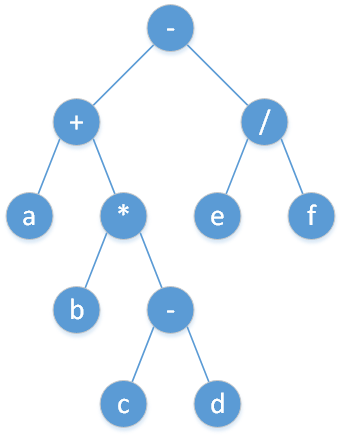
\includegraphics[width=0.7\textwidth]{docs/basic/images/bet.png} 

\end{figure}

表达式树上进行  树的遍历  可以得到不同类型的表达式

\begin{itemize}
\item 前序遍历对应前缀表达式(波兰式)
\item 中序遍历对应中缀表达式
\item 后序遍历对应后缀表达式(逆波兰式)
\end{itemize}

\subsection{非递归}

非递归的方法是定义两个  栈  来分别存储运算符和运算数。每当遇到一个数直接放进数的栈;每当遇到一个操作符时,要查找之前运算符栈中的元素,按照预先定义好的优先级来进行适当的弹出操作(弹出的同时求出对应的子表达式的值)。

我们要知道:算术表达式分为三种,分别是前缀表达式、中缀表达式、后缀表达式。其中,中缀表达式是我们日常生活中最常用的表达式;后缀表达式是计算机最容易理解的表达式。为什么说后缀表达式最容易被计算机理解呢?因为后缀表达式不需要括号表示,它的运算顺序是唯一确定的。举个例子:在后缀表达式 $3 2 * 1 -$ 中,首先计算 $3 \times 2 = 6$(使用最后一个运算符,即栈顶运算符),然后计算 $6 - 1 = 5$。可以看到:对于一个后缀表达式,只需要 \textbf{ 维护一个数字栈,每次遇到一个运算符,就取出两个栈顶元素,将运算结果重新压入栈中 }。最后,栈中唯一一个元素就是改后缀表达式的运算结果时间复杂度 $O(n)$。

所以说,对于普通中缀表达式的计算,我们可以将其转化为后缀表达式再进行计算。转换方法也十分简单。只要建立一个用于存放运算符的栈,扫描该中缀表达式:

\begin{enumerate}
\item 如果遇到数字,直接将该数字输出到后缀表达式(以下部分用「输出」表示输出到后缀表达式)
\item 如果遇到左括号,入栈
\item 如果遇到右括号,不断输出栈顶元素,直至遇到左括号。(左括号出栈,但不输出)
\item 如果遇到其他运算符,不断去除所有运算优先级大于等于当前运算符的运算符,输出。最后,新的符号入栈。
\item 把栈中剩下的符号依次输出,表达式转换结束。
\end{enumerate}

时间复杂度 $O(n)$.

示例代码:

\begin{cppcode}
// 下面代码摘自笔者 NOIP2005 等价表达式
std::string convert(const std::string &s) {  // 把中缀表达式转换为后缀表达式
  std::stack<char> oper;
  std::stringstream ss;
  ss << s;
  std::string t, tmp;
  while (ss >> tmp) {
    if (isdigit(tmp[0]))
      t += tmp + " ";  // 1. 如果遇到一个数,输出该数
    else if (tmp[0] == '(')
      oper.push(tmp[0]);       // 2. 如果遇到左括号,把左括号入栈
    else if (tmp[0] == ')') {  // 3. 如果遇到右括号,
      while (!oper.empty() && oper.top() != '(')
        t += std::string(1, oper.top()) + " ",
            oper.pop();  // 不断取出栈顶并输出,直到栈顶为左括号,
      oper.pop();        // 然后把左括号出栈
    } else {             // 4. 如果遇到运算符
      while (!oper.empty() && level[oper.top()] >= level[tmp[0]])
        t += std::string(1, oper.top()) + " ",
            oper.pop();  // 只要栈顶符号的优先级不低于新符号,就不断取出栈顶并输出
      oper.push(tmp[0]);  // 最后把新符号进栈
    }
  }
  while (!oper.empty()) t += std::string(1, oper.top()) + " ", oper.pop();
  return t;
}

int calc(const std::string &s) {  // 计算转换好的后缀表达式
  std::stack<int> num;
  std::stringstream ss;
  ss << s;
  std::string t, tmp;
  while (ss >> tmp) {
    if (isdigit(tmp[0]))
      num.push(stoi(tmp));
    else {
      int b, a;  // 取出栈顶元素,注意顺序
      if (!num.empty()) b = num.top();
      num.pop();
      if (!num.empty()) a = num.top();
      num.pop();
      if (tmp[0] == '+') num.push(a + b);
      if (tmp[0] == '-') num.push(a - b);
      if (tmp[0] == '*') num.push(a * b);
      if (tmp[0] == '^') num.push(qpow(a, b));
    }
  }
  return num.top();
}
\end{cppcode}

\subsection{习题}

\begin{enumerate}
\item \href{https://www.luogu.org/problemnew/show/P1981}{表达式求值 (NOIP2013)}
\item \href{https://www.luogu.org/problemnew/show/P1449}{后缀表达式}
\item \href{https://www.spoj.com/problems/ONP/}{Transform the Expression}
\end{enumerate}

\section{二分}

\subsection{二分搜索}

二分搜索,也称折半搜索,是用来在一个有序数组中查找某一元素的算法。

以在一个升序数组中查找一个数为例。

它每次考察数组当前部分的中间元素,如果中间元素刚好是要找的,就结束搜索过程;如果中间元素小于所查找的值,那么左侧的只会更小,不会有所查找的元素,只需要到右侧去找就好了;如果中间元素大于所查找的值,同理,右侧的只会更大而不会有所查找的元素,所以只需要到左侧去找。

在二分搜索过程中,每次都把查询的区间减半,因此对于一个长度为 $n$ 的数组,至多会进行 $O(\log n)$ 次查找。

\begin{cppcode}
int binary_search(int start, int end, int key) {
  int ret = -1;  // 未搜索到数据返回-1下标
  int mid;
  while (start <= end) {
    mid = start + ((end - start) >> 1);  //直接平均可能会溢出,所以用这个算法
    if (arr[mid] < key)
      start = mid + 1;
    else if (arr[mid] > key)
      end = mid - 1;
    else {  // 最后检测相等是因为多数搜索情况不是大于就是小于
      ret = mid;
      break;
    }
  }
  return ret;  // 单一出口
}
\end{cppcode}

\begin{NOTE}{}{}
\texttt{>> 1} 比 \texttt{/ 2} 速度快一些

\end{NOTE}


注意,这里的有序是广义的有序,如果一个数组中的左侧或者右侧都满足某一种条件,而另一侧都不满足这种条件,也可以看作是一种有序(如果把满足条件看做 $1$,不满足看做 $0$,至少对于这个条件的这一维度是有序的)。换言之,二分搜索法可以用来查找满足某种条件的最大(最小)的值。

如果我们要求满足某种条件的最大值的最小可能情况(最大值最小化)呢?首先的想法是从小到大枚举这个作为答案的「最大值」,然后去判断是否合法。要是这个答案是单调的就好了,那样就可以使用二分搜索法来更快地找到答案。

要想使用二分搜索法来解这种「最大值最小化」的题目,需要满足以下三个条件:

\begin{enumerate}
\item 答案在一个固定区间内;
\item 可能查找一个符合条件的值不是很容易,但是要求能比较容易地判断某个值是否是符合条件的;
\item 可行解对于区间满足一定的单调性。换言之,如果 $x$ 是符合条件的,那么有 $x + 1$ 或者 $x - 1$ 也符合条件。(这样下来就满足了上面提到的单调性)
\end{enumerate}

当然,最小值最大化是同理的。

二分法把一个寻找极值的问题转化成一个判定的问题(用二分搜索来找这个极值)。类比枚举法,我们当时是枚举答案的可能情况,现在由于单调性,我们不再需要一个个枚举,利用二分的思路,就可以用更优的方法解决「最大值最小」、「最小值最大」。这种解法也成为是「二分答案」,常见于解题报告中。

\subsubsection{STL 的二分查找}

补充一个小知识点, 对于一个有序的 array 你可以使用 \texttt{std::lower\_bound()} 来找到第一个大于等于你的值的数, \texttt{std::upper\_bound()} 来找到第一个大于你的值的数。

请注意,必须是有序数组,否则答案是错误的。

关于具体使用方法,请参见  STL 页面 。

\subsection{三分法}

\begin{cppcode}
mid = left + (right - left >> 1);
midmid = mid + (right - mid >> 1);  // 对右侧区间取半
if (cal(mid) > cal(midmid))
  right = midmid;
else
  left = mid;
\end{cppcode}

三分法可以用来查找凸函数的最大(小)值。

画一下图好理解一些(图待补)

\begin{itemize}
\item 如果 \texttt{mid} 和 \texttt{midmid} 在最大(小)值的同一侧:
那么由于单调性,一定是二者中较大(小)的那个离最值近一些,较远的那个点对应的区间不可能包含最值,所以可以舍弃。
\item 如果在两侧:
由于最值在二者中间,我们舍弃两侧的一个区间后,也不会影响最值,所以可以舍弃。
\end{itemize}

\subsection{分数规划}

分数规划是这样一类问题,每个物品有两个代价 $c_i$,$d_i$,要求通过某种方式选出若干个,使得 $\frac{\sum{c_i}}{\sum{d_i}}$ 最大或最小。

经典的例子是 最优比率环、最优比率生成树 等等。

\subsubsection{二分法}

比如说我们要求的是最小的,记 $L$ 为最优的答案,对这个式子做一些变换:

$$
L \geq \frac{\sum{c_i}}{\sum{d_i}}
$$

把分母乘过去,把右侧化为 $0$:

$$
{\sum{d_i}} \times L - {\sum{c_i}} \geq 0
$$

即:

$$
{\sum_{i=1}^N{d_i}} \times L - {\sum_{i=1}^N{c_i}} \geq 0
$$

$$
\sum_{i=1}^N{d_i \times L - c_i} \geq 0
$$

不难发现,如果 $L'$ 比 $L$ 要小,上式左端的值会更大一些。

所以要求得最小的 $L$,我们要求的就变成了让上式左端最接近 $0$ 的 $L$。

不难发现左端的式子是随 $L$ 变化而单调变化的,所以可以通过二分法来解决。

\subsubsection{Dinkelbach 算法}

Dinkelbach 算法是每次用上一轮的答案当做新的 $L$ 来输入,不断地迭代,直至答案收敛。

\section{构造}

构造题是比赛中常见的一类题型。

从形式上来看,问题的答案往往具有某种规律性,使得在问题规模迅速增大的时候,仍然有机会比较容易地得到答案。

这要求我们在解题时,要思考问题规模增长对答案的影响,这种影响是否可以推广。(比如在设计动态规划方法的时候,要考虑从一个状态到后继状态的转移会造成什么影响)。

\section{前缀和 \& 差分}

\subsection{前缀和}

前缀和是一种较为简单的算法,可以大大减少时间复杂度。我们可以简单理解为 “数列的前 n 项的和”。下面我们用一个例题来了解一下前缀和的主要思路。

\begin{NOTE}{例题}{}
有 N 个的正整数放到数组 A 里,现在要求一个新的数组 B,新数组的第 i 个数 B[i] 是原数组 A 第 0 到第 i 个数的和。

\end{NOTE}


对于这道题,我们有两种做法:

\begin{itemize}
\item 把对数组 A 的累加依次放入数组 B 中。
\item 递推:\texttt{B[i] = B[i-1] + A[i]} ,前提 \texttt{B[0] = A[0]}。
\end{itemize}

参考程序:

\begin{cppcode}
#include <iostream>

using namespace std;

int N, A[10000], B[10000];
int main() {
  cin >> N;
  for (int i = 0; i < N; i++) {
    cin >> A[i];
  }

  B[0] = A[0];

  for (int i = 1; i < N; i++) {
    B[i] = B[i - 1] + A[i];
  }

  for (int i = 0; i < N; i++) {
    cout << B[i] << " ";
  }

  return 0;
}
\end{cppcode}

输入:

\begin{minted}{text}
5
1 2 3 4 5
\end{minted}

输出:

\begin{minted}{text}
1 3 6 10 15 
\end{minted}

首先,\texttt{B[0] = A[0];},前缀和数组的第一项和原数组的第一项是相等的。

\texttt{B[i] = B[i-1] + A[i]} 相信大家也能理解这个式子。意思就是:前缀和数组的第 i 项等于数组 A 的 0 到 i-1 项的和加数组 A 的第 i 项。

\subsubsection{参考}

感谢南海区青少年信息学奥林匹克内部训练教材。

\section{文件操作}

\subsection{文件的概念}

文件是根据特定的目的而收集在一起的有关数据的集合。C/C++ 把每一个文件都看成是一个有序的字节流,每个文件都是以\textbf{文件结束标志}(EOF)结束,如果要操作某个文件,程序应该首先打开该文件,每当一个文件被打开后(请记得关闭打开的文件),该文件就和一个流关联起来,这里的流实际上是一个字节序列。  

C/C++ 将文件分为文本文件和二进制文件。文本文件就是简单的文本文件(重点),另外二进制文件就是特殊格式的文件或者可执行代码文件等。

\subsection{文件的操作步骤}

 1、打开文件,将文件指针指向文件,决定打开文件类型;  

 2、对文件进行读、写操作(比赛中主要用到的操作,其他一些操作暂时不写);  

 3、在使用完文件后,关闭文件。  

\subsection{\texttt{freopen} 函数}

\subsubsection{命令格式}

\begin{cppcode}
FILE* freopen(const char* filename, const char* mode, FILE* stream);
\end{cppcode}

\subsubsection{参数说明}

\begin{itemize}
\item \texttt{filename}: 要打开的文件名
\item \texttt{mode}: 文件打开的模式
\item \texttt{stream}: 文件指针,通常使用标准文件流 (\texttt{stdin/stdout/stderr})  
\end{itemize}

\subsubsection{使用方法}

读入文件内容:

\begin{cppcode}
freopen("data.in", "r", stdin);
// data.in 就是读取的文件名,要和可执行文件放在同一目录下
\end{cppcode}

输出到文件:

\begin{cppcode}
freopen("data.out", "w", stdout);
// data.out 就是输出文件的文件名,和可执行文件在同一目录下
\end{cppcode}

关闭标准输入 / 输出流  

\begin{cppcode}
fclose(stdin);
fclose(stdout);
\end{cppcode}

\subsubsection{模板}

\begin{cppcode}
#include <cstdio>
#include <iostream>
int main(void) {
  freopen("data.in", "r", stdin);
  freopen("data.out", "w", stdout);
  /*
  中间的代码不需要改变,直接使用 cin 和 cout 即可
  */
  fclose(stdin);
  fclose(stdout);
  return 0;
}
\end{cppcode}

参考书目:信息学奥赛一本通

\subsection{C++ 的 ifstream/ofstream 文件输入输出流}

\subsubsection{使用方法}

读入文件内容:

\begin{cppcode}
ifstream fin("data.in");
// data.in 就是读取的文件名,要和可执行文件放在同一目录下
\end{cppcode}

输出到文件:

\begin{cppcode}
ofstream fout("data.out");
// data.out 就是输出文件的文件名,和可执行文件在同一目录下
\end{cppcode}

关闭标准输入  输出流

\begin{cppcode}
fin.close();
fout.close();
\end{cppcode}

\subsubsection{模板}

\begin{cppcode}
#include <cstdio>
#include <fstream>
ifstream fin("data.in");
ofstream fout("data.out");
int main(void) {
  /*
  中间的代码改变 cin 为 fin ,cout 为 fout 即可
  */
  fin.close();
  fout.close();
  return 0;
}
\end{cppcode}

\chapter{搜索}
\section{搜索部分简介}

搜索的思想按照在状态空间中尝试的顺序分为多种。搜索看起来简单,但是往往是很多复杂的题目中必不可少的模块。

\subsection{深度优先搜索 (DFS)}

主条目: DFS 

优先深入遍历靠前的节点,可以用堆栈实现。

\subsection{宽度优先搜索 (BFS)}

主条目: BFS 

优先扩展浅层节点,逐渐深入,可以用队列实现。

\subsubsection{双向宽度优先搜索}

主条目: 双向广搜 

从状态图上起点和终点同时开始进行宽度优先搜索,如果发现相遇了,那么可以认为是获得了可行解。

\subsection{A 搜索}

主条目: A 

\subsection{IDA 搜索}

主条目: IDA 

\subsection{剪枝}

搜索往往是在庞大的解空间中尝试获得最优解,这时候剪枝就显得十分必要了。剪枝顾名思义,是运用已有的信息,尽早地确定一种方案是否可行,如果已经知道无法获得最优解就及时退回。这样的操作对于搜索树来说,就相当于是在搜索树上剪掉一些枝杈。

剪枝思路有很多种,大多需要对于具体问题来分析,在此简要介绍几种常见的剪枝思路。

\subsubsection{极端法}

考虑极端情况,如果最极端(最理想)的情况都无法满足,那么肯定实际情况搜出来的结果不会更优了。

\subsubsection{调整法}

通过对子树的比较剪掉重复子树和明显不是最有 “前途” 的子树。

\subsubsection{数学方法}

比如在图论中借助连通分量,数论中借助模方程的分析,借助不等式的放缩来估计下界等等。

\subsection{meet-in-middle 分治}

也称折半搜索,主要思想是分治,通过将枚举量减少到原来的一半和特殊的合并技巧以使情况数减少到原来的 sqrt,复杂度也就开了个方,折半搜索也是一个很好的优化,往往能在 OI 竞赛中获得出人意料的效果(尤其在面对数据水的时候)

所谓 \textbf{meet-in-middle} , 就是让 dfs 的状态在中间的时候碰面。我们知道, 如果一个暴力 dfs 有 $K$ 个转移, 那么它的时间复杂度 (大多数情况) 是 $O(K^N)$ 的。那我们就想, 当 $N$ 到达一定程度时, TLE 会变成必然。

例题 \href{https://www.luogu.org/problemnew/show/P2962}{luogu P2962  灯 Lights}

我们正常想, 如果这道题暴力 dfs 找开关灯的状态, 时间复杂度就是 $O(2^{35})$, 显然超时。不过, 如果我们用 \textbf{meet-in-middle} 的话, 时间复杂度将会变为 $O(2^{18} \times 2)$ 而已。

 \textbf{meet-in-middle} 就是让我们先找一半的状态, 也就是 $1$ 到 $mid$ ($N$ 的一半) 的状态, 再找剩下的状态就可以了。我们把前半段的状态全部存储在 $hash$ 表或者 $map$ 里面, 然后在找后半段的状态的时候, 先判断后半段是不是都合法, 就可以判断上半段有没有配对的上半段使得整段合法。

\section{DFS}

DFS 全称是 \href{https://en.wikipedia.org/wiki/Depth-first_search}{Depth First Search}。

是一种图的遍历算法。

所谓深度优先。就是说每次都尝试向更深的节点走。

如果没有更深的节点了,就回到上一层的下一个节点继续刚才的过程。

上面的解释太过高深,我们可以感性地理解一下它,在较为初级的应用(非图论)中,搜索就是一个暴力枚举,

如这个例子:

\begin{QUOTE}{}{}
把正整数 n 分解为 3 个不同的数,如 6=1+2+3 排在后面的数必须大于等于前面的数



对于这个问题,如果不知道搜索,应该怎么办呢?



当然是 3 重循环 伪代码如下



\begin{minted}{text}

for i=1..n

  for j=i..n

    for k=1..n

      if (i+j+k=n) printf("%d=%d+%d+%d",n,i,j,k);

\end{minted}



那如果是分解成四个整数呢?



再加一重循环?
\end{QUOTE}

那分解成小于等于 m 个整数呢?

if 一大堆,写 m 个?

这时候就需要用到搜索了。

上面的例子也可以抽象成图,就是把能分解的数都算作一个点,然后按顺序把他们连起来。

\subsection{模板}

不管是图还是其它,都是这样

伪代码:

\begin{minted}{text}
dfs(n) {
  if (碰到边界) //如上面例子中的分解完就是基本情况
    返回 值,并退出
  for i=可以继续搜下去的情况
    if(可以){
      标记为不可以
      dfs(i);//继续往下搜
      标回可以
    }
}
\end{minted}

有些情况不需要标记,请自行判断。

\subsection{实现(对于图来说)}

伪代码:

\begin{minted}{text}
dfs(u) {
  visited[u] = true
  for each edge(u, v) {
    if (!visited[v]) {
      dfs(v)
    }
  }
}
\end{minted}

C++:

\begin{cppcode}
void dfs(int u) {
  vis[u] = 1;
  for (int i = head[u]; i; i = e[i].x) {
    // 这里用到的是链式前向星来存图
    if (!vis[e[i].t]) {
      dfs(v);
    }
  }
}
\end{cppcode}

时间复杂度 $O(n + m)$。

空间复杂度 $O(n)$。 (vis 数组和递归栈)

\subsection{在树 / 图上 DFS}

主条目: 在树 / 图上 DFS 

\section{BFS}

BFS 全称是 \href{https://en.wikipedia.org/wiki/Breadth-first_search}{Breadth First Search},中文名是宽度优先搜索,也叫广度优先搜索。

是图上最基础、最重要的搜索算法之一。

所谓宽度优先。就是每次都尝试访问同一层的节点。

如果同一层都访问完了,再访问下一层。

这样做的结果是,BFS 算法找到的路径是从起点开始的 \textbf{ 最短 } 合法路径。换言之,这条路所包含的边数最小。

在 BFS 结束时,每个节点都是通过从起点到该点的最短路径访问的。

算法过程可以看做是图上火苗传播的过程:最开始只有起点着火了,在每一时刻,有火的节点都向它相邻的所有节点传播火苗。

\subsection{实现}

伪代码:

\begin{minted}{text}
bfs(s) {
  q = new queue()
  q.push(s)), visited[s] = true
  while (!q.empty()) {
    u = q.pop()
    for each edge(u, v) {
      if (!visited[v]) {
        q.push(v)
        visited[v] = true
      }
    }
  }
}
\end{minted}

C++:

\begin{cppcode}
void bfs(int u) {
  while (!Q.empty()) Q.pop();
  Q.push(u);
  vis[u] = 1;
  d[u] = 0;
  p[u] = -1;
  while (!Q.empty()) {
    u = Q.pop() {
      for (int i = head[u]; i; i = e[i].x) {
        if (!vis[e[i].t]) {
          Q.push(e[i].t);
          vis[e[i].t] = 1;
          d[e[i].t] = d[u] + 1;
          p[e[i].t] = u;
        }
      }
    }
  }
}
void restore(int x) {
  vector<int> res;
  for (int v = x; v != -1; v = p[v]) {
    res.push_back(v);
  }
  std::reverse(res.begin(), res.end());
  for (int i = 0; i < res.size(); ++i) printf("%d", res[i]);
  puts("");
}
\end{cppcode}

具体来说,我们用一个队列 Q 来记录要处理的节点,然后开一个 $vis[]$ 布尔数组来标记某个节点是否已经访问过了。

开始的时候,我们把起点 s 以外的节点的 vis 值设为 0,意思是没有访问过。然后把起点 s 放入队列 Q 中。

之后,我们每次从队列 Q 中取出队首的点 u,把 u 相邻的所有点 v 标记为已经访问过了并放入队列 Q。

直到某一时刻,队列 Q 为空,这时 BFS 结束。

在 BFS 的过程中,也可以记录一些额外的信息。比如上面的代码中,d 数组是用来记录某个点到起点的距离(要经过的最少边数),p 数组是记录从起点到这个点的最短路上的上一个点。

有了 d 数组,可以方便地得到起点到一个点的距离。

有了 p 数组,可以方便地还原出起点到一个点的最短路径。上面的 restore 函数就是在做这件事:restore(x) 输出的是从起点到 x 这个点所经过的点。

时间复杂度 $O(n + m)$

空间复杂度 $O(n)$ (vis 数组和队列)

\subsection{open-closed 表}

在实现 BFS 的时候,我们把未被访问过的节点放在一个称为 open 的容器中,而把已经访问过了的节点放在 closed 容器中。

\subsection{ 在树 / 图上 BFS }

\subsection{应用}

\begin{itemize}
\item 在一个无权图上求从起点到其他所有点的最短路径。
\item 在 $O(n+m)$ 时间内求出所有连通块。(我们只需要从每个没有被访问过的节点开始做 BFS,显然每次 BFS 会走完一个连通块)
\item 如果把一个游戏的动作看做是状态图上的一条边(一个转移),那么 BFS 可以用来找到在游戏中从一个状态到达另一个状态所需要的最小步骤。
\item 在一个边权为 0 / 1 的图上求最短路。(需要修改入队的过程,如果某条边权值为 0,且可以减小边的终点到图的起点的距离,那么把边的起点加到队列首而不是队列尾)
\item 在一个有向无权图中找最小环。(从每个点开始 BFS,在我们即将抵达一个之前访问过的点开始的时候,就知道遇到了一个环。图的最小环是每次 BFS 得到的最小环的平均值。)
\item 找到一定在 $(a, b)$ 最短路上的边。(分别从 a 和 b 进行 BFS,得到两个 d 数组。之后对每一条边 $(u, v)$,如果 $d_a[u]+1+d_b[v]=d_a[b]$,则说明该边在最短路上)
\item 找到一定在 $(a, b)$ 最短路上的点。(分别从 a 和 b 进行 BFS,得到两个 d 数组。之后对每一个点 v,如果 $d_a[u]+d_b[v]=d_a[b]$,则说明该点在最短路上)
\item 找到一条长度为偶数的最短路。(我们需要一个构造一个新图,把每个点拆成两个新点,原图的边 $(u, v)$ 变成 $((u, 0), (v, 1))$ 和 $((u, 1), (v, 0))$。对新图做 BFS,$(s, 0)$ 和 $(t, 0)$ 之间的最短路即为所求)
\end{itemize}

\subsection{例题}

\begin{itemize}
\item \href{https://loj.ac/problem/2317}{LOJ\textbackslash{}\#2317. 「NOIP2017」奶酪}
\end{itemize}

\subsection{参考}

\url{https://cp-algorithms.com/graph/breadth-first-search.html}

\subsection{双端队列 BFS}

如果你不了解双端队列 \texttt{deque} 的话,请到 STL-queue 中学习。

双端队列 BFS 又称 0-1 BFS

\subsubsection{适用范围}

边权值为可能有,也可能没有(由于 BFS 适用于权值为 1 的图,所以一般是 0 or 1),或者能够转化为这种边权值的最短路问题。

例如在走迷宫问题中,你可以花 1 个金币走 5 步,也可以不花金币走 1 步,这就可以用 0-1 BFS 解决。

\subsubsection{实现}

一般情况下,我们把没有权值的边扩展到的点放到队首,有权值的边扩展到的点放到队尾。这样即可保证在整个队列中,像普通 BFS 一样,越靠近队首,权值越小,且权值零一之间有分隔。

下面是伪代码:

\begin{cppcode}
while (队列不为空) {
  int u = 队首;
  弹出队首;
  for (枚举 u 的邻居) {
    更新数据
    if (...)
      添加到队首;
    else
      添加到队尾;
  }
}
\end{cppcode}

\subsubsection{例题}

\subsubsection{\href{http://codeforces.com/problemset/problem/173/B}{Codeforces 173B}}

一个 $n \times m$ 的图,现在有一束激光从左上角往右边射出,每遇到 '\#',你可以选择光线往四个方向射出,或者什么都不做,问最少需要多少个 '\#' 往四个方向射出才能使光线在第 $n$ 行往右边射出。

此题目正解不是 0-1 BFS 但是适用 0-1 BFS 可以不需要思考过程,赛时许多大佬都是这么做的。

做法很简单,一个方向射出不需要花费(0),而往四个方向射出需要花费(1),然后直接来就可以了。

\paragraph{Code}

\begin{cppcode}
#include <bits/stdc++.h>
using namespace std;
#define INF (1 << 29)
int n, m;
char grid[1001][1001];
int dist[1001][1001][4];
int vis[1001][1001][4];
int fx[] = {1, -1, 0, 0};
int fy[] = {0, 0, 1, -1};
deque<int> q;
void add_front(int x, int y, int dir, int d) {
  if (d < dist[x][y][dir]) {
    dist[x][y][dir] = d;
    q.push_front(dir);
    q.push_front(y);
    q.push_front(x);
  }
}
void add_back(int x, int y, int dir, int d) {
  if (d < dist[x][y][dir]) {
    dist[x][y][dir] = d;
    q.push_back(x);
    q.push_back(y);
    q.push_back(dir);
  }
}
int main() {
  cin >> n >> m;
  for (int i = 0; i < n; i++) cin >> grid[i];

  for (int i = 0; i < n; i++)
    for (int j = 0; j < m; j++)
      for (int k = 0; k < 4; k++) dist[i][j][k] = INF;

  add_front(n - 1, m - 1, 3, 0);

  while (!q.empty()) {
    int x = q[0], y = q[1], dir = q[2];
    q.pop_front();
    q.pop_front();
    q.pop_front();
    if (vis[x][y][dir]) continue;
    vis[x][y][dir] = true;
    int d = dist[x][y][dir];
    int nx = x + fx[dir], ny = y + fy[dir];
    if (nx >= 0 && nx < n && ny >= 0 && ny < m) add_front(nx, ny, dir, d);
    if (grid[x][y] == '#')
      for (int i = 0; i < 4; i++)
        if (i != dir) add_back(x, y, i, d + 1);
  }
  if (dist[0][0][3] == INF)
    cout << -1 << endl;
  else
    cout << dist[0][0][3] << endl;
  return 0;
}
\end{cppcode}

\subsection{优先队列 BFS}

优先队列,相当于一个二叉堆,STL 中提供了  \texttt{std::priority\_queue} ,可以方便我们使用优先队列。

在基于优先队列的 BFS 中,我们每次从队首取出代价最小的结点进行进一步搜索。容易证明这个贪心思想是正确的,因为从这个结点开始扩展的搜索,一定不会更新原来那些代价更高的结点。换句话说,其余那些代价更高的结点,我们不回去考虑更新它。

当然,每个结点可能会被入队多次,只是每次入队的代价不同。当该结点第一次从优先队列中取出,以后便无需再在该结点进行搜索,直接忽略即可。所以,优先队列的 BFS 当中,每个结点只会被处理一次。

相对于普通队列的 BFS,时间复杂度多了一个 $\log$,毕竟要维护这个优先队列嘛。不过普通 BFS 有可能每个结点入队、出队多次,时间复杂度会达到 $O(n^2)$,不是 $O(n)$。所以优先队列 BFS 通常还是快的。

诶?这怎么听起来这么像堆优化的  Dijkstra  算法呢?事实上,堆优化 Dijkstra 就是优先队列 BFS。

\section{双向 BFS}

从状态图上起点和终点同时开始进行宽度优先搜索,如果发现相遇了,那么可以认为是获得了可行解。

\section{启发式搜索}



\section{A*}

A 算法是  BFS  的一种改进。

定义起点 $s$,终点 $t$。

从起点(初始状态)开始的距离函数 $g(x)$。

到终点(最终状态)的距离函数 $h(x), h*(x)$。

定义每个点的估价函数 $f(x)=g(x)+h(x)$。

A 算法每次从 \textbf{优先队列} 中取出一个 $f$ 最小的,然后更新相邻的状态。

如果 $h\leq h*$,则 A 算法能找到最优解。

上述条件下,如果 $h$ \textbf{满足三角形不等式,则 A 算法不会将重复结点加入队列}。

其实…… $h=0$ 时就是  DFS  算法,$h=0$ 并且边权为 $1$ 时就是  BFS 。

\subsection{例题 \href{https://www.luogu.org/problemnew/show/P1379}{八数码}}

题目大意:在 $3\times 3$ 的棋盘上,摆有八个棋子,每个棋子上标有 1 至 8 的某一数字。棋盘中留有一个空格,空格用 0 来表示。空格周围的棋子可以移到空格中,这样原来的位置就会变成空格。给出一种初始布局和目标布局(为了使题目简单, 设目标状态为

\begin{minted}{text}
123
804
765
\end{minted}

),找到一种从初始布局到目标布局最少步骤的移动方法。

$h$ 函数可以定义为,不在应该在的位置的数字个数。

容易发现 $h$ 满足以上两个性质,此题可以使用 A 算法求解。

代码实现:

\begin{cppcode}
#include <algorithm>
#include <cstdio>
#include <cstring>
#include <queue>
#include <set>
using namespace std;
const int dx[4] = {1, -1, 0, 0}, dy[4] = {0, 0, 1, -1};
int fx, fy;
char ch;
struct matrix {
  int a[5][5];
  bool operator<(matrix x) const {
    for (int i = 1; i <= 3; i++)
      for (int j = 1; j <= 3; j++)
        if (a[i][j] != x.a[i][j]) return a[i][j] < x.a[i][j];
    return false;
  }
} f, st;
int h(matrix a) {
  int ret = 0;
  for (int i = 1; i <= 3; i++)
    for (int j = 1; j <= 3; j++)
      if (a.a[i][j] != st.a[i][j]) ret++;
  return ret;
}
struct node {
  matrix a;
  int t;
  bool operator<(node x) const { return t + h(a) > x.t + h(x.a); }
} x;
priority_queue<node> q;
set<matrix> s;
int main() {
  st.a[1][1] = 1;
  st.a[1][2] = 2;
  st.a[1][3] = 3;
  st.a[2][1] = 8;
  st.a[2][2] = 0;
  st.a[2][3] = 4;
  st.a[3][1] = 7;
  st.a[3][2] = 6;
  st.a[3][3] = 5;
  for (int i = 1; i <= 3; i++)
    for (int j = 1; j <= 3; j++) {
      scanf(" %c", &ch);
      f.a[i][j] = ch - '0';
    }
  q.push({f, 0});
  while (!q.empty()) {
    x = q.top();
    q.pop();
    if (!h(x.a)) {
      printf("%d\n", x.t);
      return 0;
    }
    for (int i = 1; i <= 3; i++)
      for (int j = 1; j <= 3; j++)
        if (!x.a.a[i][j]) fx = i, fy = j;
    for (int i = 0; i < 4; i++) {
      int xx = fx + dx[i], yy = fy + dy[i];
      if (1 <= xx && xx <= 3 && 1 <= yy && yy <= 3) {
        swap(x.a.a[fx][fy], x.a.a[xx][yy]);
        if (!s.count(x.a)) s.insert(x.a), q.push({x.a, x.t + 1});
        swap(x.a.a[fx][fy], x.a.a[xx][yy]);
      }
    }
  }
  return 0;
}
\end{cppcode}

\subsection{例题 \href{https://www.luogu.org/problemnew/show/P2483}{k 短路}}

题目大意:按顺序求一个有向图上从结点 $s$ 到结点 $t$ 的所有路径最小的前任意多(不妨设为 $k$ )个。

很容易发现,这个问题很容易转化成用 A 算法解决问题的标准程式。

初始状态为处于结点 $s$,最终状态为处于结点 $t$,距离函数为从 $s$ 到当前结点已经走过的距离,估价函数为从当前结点到结点 $t$ 至少要走过的距离,也就是当前结点到结点 $t$ 的最短路。

就这样,我们在预处理的时候反向建图,计算出结点 $t$ 到所有点的最短路,然后将初始状态塞入优先队列,每次取出 $f(x)=g(x)+h(x)$ 最小的一项,计算出其所连结点的信息并将其也塞入队列。当你第 $k$ 次走到结点 $t$ 时,也就算出了结点 $s$ 到结点 $t$ 的 $k$ 短路。

由于设计的距离函数和估价函数,每个状态需要存储两个参数,当前结点 $x$ 和已经走过的距离 $v$。

我们可以在此基础上加一点小优化:由于只需要求出第 $k$ 短路,所以当我们第 $k+1$ 次或以上走到该结点时,直接跳过该状态。因为前面的 $k$ 次走到这个点的时候肯定能因此构造出 $k$ 条路径,所以之后在加边更无必要。

代码实现:

\begin{cppcode}
#include <algorithm>
#include <cstdio>
#include <cstring>
#include <queue>
using namespace std;
const int maxn = 5010;
const int maxm = 400010;
const double inf = 2e9;
int n, m, k, u, v, cur, h[maxn], nxt[maxm], p[maxm], cnt[maxn], ans;
int cur1, h1[maxn], nxt1[maxm], p1[maxm];
double e, ww, w[maxm], f[maxn];
double w1[maxm];
bool tf[maxn];
void add_edge(int x, int y, double z) {
  cur++;
  nxt[cur] = h[x];
  h[x] = cur;
  p[cur] = y;
  w[cur] = z;
}
void add_edge1(int x, int y, double z) {
  cur1++;
  nxt1[cur1] = h1[x];
  h1[x] = cur1;
  p1[cur1] = y;
  w1[cur1] = z;
}
struct node {
  int x;
  double v;
  bool operator<(node a) const { return v + f[x] > a.v + f[a.x]; }
};
priority_queue<node> q;
struct node2 {
  int x;
  double v;
  bool operator<(node2 a) const { return v > a.v; }
} x;
priority_queue<node2> Q;
int main() {
  scanf("%d%d%lf", &n, &m, &e);
  while (m--) {
    scanf("%d%d%lf", &u, &v, &ww);
    add_edge(u, v, ww);
    add_edge1(v, u, ww);
  }
  for (int i = 1; i < n; i++) f[i] = inf;
  Q.push({n, 0});
  while (!Q.empty()) {
    x = Q.top();
    Q.pop();
    if (tf[x.x]) continue;
    tf[x.x] = true;
    f[x.x] = x.v;
    for (int j = h1[x.x]; j; j = nxt1[j]) Q.push({p1[j], x.v + w1[j]});
  }
  k = (int)e / f[1];
  q.push({1, 0});
  while (!q.empty()) {
    node x = q.top();
    q.pop();
    cnt[x.x]++;
    if (x.x == n) {
      e -= x.v;
      if (e < 0) {
        printf("%d\n", ans);
        return 0;
      }
      ans++;
    }
    for (int j = h[x.x]; j; j = nxt[j])
      if (cnt[p[j]] <= k && x.v + w[j] <= e) q.push({p[j], x.v + w[j]});
  }
  printf("%d\n", ans);
  return 0;
}
\end{cppcode}

\section{迭代加深搜索}

\subsection{简介}

迭代加深是一种\textbf{每次限制搜索深度的}深度优先搜索。

它的本质还是深度优先搜索,只不过在搜索的同时带上了一个深度 $d$,当 $d$ 达到设定的深度时就返回,一般用于找最优解。如果一次搜索没有找到合法的解,就让设定的深度 $+1$,重新从根开始。

既然是为了找最优解,为什么不用 BFS 呢?我们知道 BFS 的基础是一个队列,队列的空间复杂度很大,当状态比较多或者单个状态比较大时,使用队列的 BFS 就显出了劣势。事实上,迭代加深就类似于用 DFS 方式实现的 BFS,它的空间复杂度相对较小。

当搜索树的分支比较多时,每增加一层的搜索复杂度会出现指数级爆炸式增长,这时前面重复进行的部分所带来的复杂度几乎可以忽略,这也就是为什么迭代加深是可以近似看成 BFS 的。

\subsection{步骤}

首先设定一个较小的深度作为全局变量,进行 DFS。每进入一次 DFS,将当前深度 $d++$,当发现 $d$ 大于设定的深度就返回。如果在搜索的途中发现了答案就可以回溯,同时在回溯的过程中可以记录路径。如果没有发现答案,就返回到函数入口,增加设定深度,继续搜索。

\subsection{代码结构}

\begin{minted}{text}
IDDFS(u,d)
    if d>设定深度
        return
    else
        for each edge (u,v)
            IDDFS(v,d+1)
  return
\end{minted}

\subsection{注意事项}

在大多数的题目中,广度优先搜索还是比较方便的,而且容易判重。当发现广度优先搜索在空间上不够优秀,而且要找最优解的问题时,就应该考虑迭代加深。

\section{IDA*}

学习 IDA 之前,请确保您已经学完了  A  算法和  迭代加深搜索  。

\subsection{IDA 简介}

IDA,即采用迭代加深的 A 算法。相对于 A 算法,由于 IDA 改成了深度优先的方式,所以 IDA 更实用:

\begin{enumerate}
\item 不需要判重,不需要排序;
\item 空间需求减少。
\end{enumerate}

\textbf{大致框架}(伪代码):

\begin{minted}{text}
Procedure IDA_STAR(StartState)
Begin
PathLimit := H(StartState) - 1;
Succes := False;
Repeat
inc(PathLimit);
StartState.g = 0;
Push(OpenStack , StartState);
Repeat
CurrentState := Pop(OpenStack);
If Solution(CurrentState) then
Success = True
Elseif PathLimit >= CurrentState.g + H(CurrentState) then
For each Child(CurrentState) do
Push(OpenStack , Child(CurrentState));
until Successor empty(OpenStack);
until Success or ResourceLimtsReached;
end;
\end{minted}

\subsubsection{优点}

\begin{enumerate}
\item 空间开销小,每个深度下实际上是一个深度优先搜索,不过深度有限制,而 DFS 的空间消耗小是众所周知的;
\item 利于深度剪枝。
\end{enumerate}

\subsubsection{缺点}

重复搜索:回溯过程中每次 depth 变大都要再次从头搜索。

\begin{QUOTE}{}{}
其实,前一次搜索跟后一次相差是微不足道的。
\end{QUOTE}

\subsection{例题}

\begin{NOTE}{埃及分数}{}
\textbf{题目描述}

在古埃及,人们使用单位分数的和(即 $\frac{1}{a}$,$a$ 是自然数)表示一切有理数。例如,$\frac{2}{3}=\frac{1}{2}+\frac{1}{6}$,但不允许 $\frac{2}{3}=\frac{1}{3}+\frac{1}{3}$,因为在加数中不允许有相同的。 

对于一个分数 $\frac{a}{b}$ ,表示方法有很多种,其中加数少的比加数多的好,如果加数个数相同,则最小的分数越大越好。 例如,$\frac{19}{45}=\frac{1}{5}+\frac{1}{6}+\frac{1}{18}$ 是最优方案。 

输入整数 $a,b$ ($0<a<b<500$),试编程计算最佳表达式。

输入样例:

\begin{minted}{text}
495 499
\end{minted}

输出样例:

\begin{minted}{text}
Case 1: 495/499=1/2+1/5+1/6+1/8+1/3992+1/14970
\end{minted}

\end{NOTE}


\textbf{分析}

这道题目理论上可以用回溯法求解,但是\textbf{解答树}会非常 “恐怖”—不仅深度没有明显的上界,而且加数的选择理论上也是无限的。换句话说,如果用宽度优先遍历,连一层都扩展不完,因为每一层都是\textbf{无限大}的。

解决方案是采用迭代加深搜索:从小到大枚举深度上限 $maxd$,每次执行只考虑深度不超过 $maxd$ 的节点。这样,只要解的深度优先,则一定可以在有限时间内枚举到。

深度上限 $maxd$ 还可以用来\textbf{剪枝}。 按照分母递增的顺序来进行扩展,如果扩展到 i 层时,前 $i$ 个分数之和为 $\frac{c}{d}$,而第 $i$ 个分数为 $\frac{1}{e}$ ,则接下来至少还需要 $\frac{\frac{a}{b}-\frac{c}{d}}{\frac{1}{e}}$ 个分数,总和才能达到 $\frac{a}{b}$ 。 例如,当前搜索到 $\frac{19}{45}=\frac{1}{5}+\frac{1}{100}+\cdots$ ,则后面的分数每个最大为 $\frac{1}{101}$,至少需要 $\frac{\frac{19}{45}-\frac{1}{5}}{\frac{1}{101}}=23$ 项总和才能达到 $\frac{19}{45}$ ,因此前 $22$ 次迭代是根本不会考虑这棵子树的。这里的关键在于:可以估计至少还要多少步才能出解。 

注意,这里的估计都是乐观的,因为用了\textbf{至少}这个词。 说得学术一点,设深度上限为 $maxd$,当前结点 $n$ 的深度为 $g(n)$,乐观估价函数为 $h(n)$,则当 $g(n)+h(n)>maxd$ 时应该剪枝。 这样的算法就是 IDA。 当然,在实战中不需要严格地在代码里写出 $g(n)$ 和 $h(n)$ ,只需要像刚才那样设计出乐观估价函数,想清楚在什么情况下不可能在当前的深度限制下出解即可。

\begin{QUOTE}{}{}
如果可以设计出一个乐观估价函数,预测从当前结点至少还需要扩展几层结点才有可能得到解,则迭代加深搜索变成了 IDA 算法。
\end{QUOTE}

\textbf{代码}

\begin{cppcode}
// 埃及分数问题
#include <algorithm>
#include <cassert>
#include <cstdio>
#include <cstring>
#include <iostream>
using namespace std;

int a, b, maxd;

typedef long long LL;

LL gcd(LL a, LL b) { return b == 0 ? a : gcd(b, a % b); }

// 返回满足1/c <= a/b的最小c
inline int get_first(LL a, LL b) { return b / a + 1; }

const int maxn = 100 + 5;

LL v[maxn], ans[maxn];

// 如果当前解v比目前最优解ans更优,更新ans
bool better(int d) {
  for (int i = d; i >= 0; i--)
    if (v[i] != ans[i]) {
      return ans[i] == -1 || v[i] < ans[i];
    }
  return false;
}

// 当前深度为d,分母不能小于from,分数之和恰好为aa/bb
bool dfs(int d, int from, LL aa, LL bb) {
  if (d == maxd) {
    if (bb % aa) return false;  // aa/bb必须是埃及分数
    v[d] = bb / aa;
    if (better(d)) memcpy(ans, v, sizeof(LL) * (d + 1));
    return true;
  }
  bool ok = false;
  from = max(from, get_first(aa, bb));  // 枚举的起点
  for (int i = from;; i++) {
    // 剪枝:如果剩下的maxd+1-d个分数全部都是1/i,加起来仍然不超过aa/bb,则无解
    if (bb * (maxd + 1 - d) <= i * aa) break;
    v[d] = i;
    // 计算aa/bb - 1/i,设结果为a2/b2
    LL b2 = bb * i;
    LL a2 = aa * i - bb;
    LL g = gcd(a2, b2);  // 以便约分
    if (dfs(d + 1, i + 1, a2 / g, b2 / g)) ok = true;
  }
  return ok;
}

int main() {
  int kase = 0;
  while (cin >> a >> b) {
    int ok = 0;
    for (maxd = 1; maxd <= 100; maxd++) {
      memset(ans, -1, sizeof(ans));
      if (dfs(0, get_first(a, b), a, b)) {
        ok = 1;
        break;
      }
    }
    cout << "Case " << ++kase << ": ";
    if (ok) {
      cout << a << "/" << b << "=";
      for (int i = 0; i < maxd; i++) cout << "1/" << ans[i] << "+";
      cout << "1/" << ans[maxd] << "\n";
    } else
      cout << "No solution.\n";
  }
  return 0;
}
\end{cppcode}

\subsection{练习题}

\href{https://www.luogu.org/problem/show?pid=uva1343}{旋转游戏 UVa1343}

\section{回溯法}



\section{Dancing Links}



\section{优化}

\subsection{前言}

dfs(即 深搜)是一种常见的算法,大部分的题目都可以用 dfs 解决,但是大部分情况下,这都是骗分算法,很少会有爆搜为正解的题目。因为 dfs 的时间复杂度特别高。(没学过 dfs 的请自行补上这一课)

既然不能成为正解,那就多骗一点分吧。那么这一篇文章将介绍一些实用的优化算法(俗称 “剪枝”)。

先来一段深搜模板,之后的模板将在此基础上进行修改。

\begin{cppcode}
int ans = 最坏情况, now;  // now为当前答案
void dfs(传入数值) {
  if (到达目的地) ans = 从当前解与已有解中选最优;
  for (遍历所有可能性)
    if (可行) {
      进行操作;
      dfs(缩小规模);
      撤回操作;
    }
}
\end{cppcode}

其中的 ans 可以是解的记录,那么从当前解与已有解中选最优就变成了输出解.

\subsection{优化与剪枝}

最常用的剪枝有 3 种,记忆化搜索、最优性剪枝、可行性剪枝。

\subsubsection{记忆化搜索}

因为在搜索中,相同的传入值往往会带来相同的解,那我们就可以用数组来记忆,详见 记忆化搜索 。

\textbf{模板:}

\begin{cppcode}
int g[MAXN];  //定义记忆化数组
int ans = 最坏情况, now;
void dfs f(传入数值) {
  if (g[规模] != 无效数值) return;  //或记录解,视情况而定
  if (到达目的地) ans = 从当前解与已有解中选最优;  //输出解,视情况而定
  for (遍历所有可能性)
    if (可行) {
      进行操作;
      dfs(缩小规模);
      撤回操作;
    }
}
int main() {
  ... memset(g, 无效数值, sizeof(g));  //初始化记忆化数组
  ...
}
\end{cppcode}

\subsubsection{最优性剪枝}

在搜索中导致运行慢的原因还有一种,就是在当前解已经比已有解差时仍然在搜索,那么我们只需要判断一下当前解是否已经差于已有解。

\textbf{模板:}

\begin{cppcode}
int ans = 最坏情况, now;
void dfs(传入数值) {
  if (now比ans的答案还要差) return;
  if (到达目的地) ans = 从当前解与已有解中选最优;
  for (遍历所有可能性)
    if (可行) {
      进行操作;
      dfs(缩小规模);
      撤回操作;
    }
}
\end{cppcode}

\subsubsection{可行性剪枝}

\textbf{模板:}

在搜索中如果当前解已经不可用了还运行,也是在搜索中导致运行慢的原因。

\begin{cppcode}
int ans = 最坏情况, now;
void dfs(传入数值) {
  if (当前解已不可用) return;
  if (到达目的地) ans = 从当前解与已有解中选最优;
  for (遍历所有可能性)
    if (可行) {
      进行操作;
      dfs(缩小规模);
      撤回操作;
    }
}
\end{cppcode}

\chapter{动态规划}
\section{动态规划部分简介}

动态规划应用于子问题重叠的情况:

\begin{enumerate}
\item 要去刻画最优解的结构特征;
\item 尝试递归地定义最优解的值(就是我们常说的考虑从 $i - 1$ 转移到 $i$);
\item 计算最优解;
\item 利用计算出的信息构造一个最优解。
\end{enumerate}

\subsection{钢条切割}

给定一段钢条,和不同长度的价格,问如何切割使得总价格最大。

为了求解规模为 $n$ 的原问题,我们先求解形式完全一样,但规模更小的子问题。

即当完成首次切割后,我们将两段钢条看成两个独立的钢条切割问题实例。

我们通过组合相关子问题的最优解,并在所有可能的两段切割方案中选取组合收益最大者,构成原问题的最优解。

\begin{QUOTE}{}{}
最优子结构:问题的最优解由相关子问题的最优解组合而成,而这些子问题可以独立求解。
\end{QUOTE}

动态规划的两种实现方法:

\begin{itemize}
\item 带备忘的自顶向下法 (记忆化搜索);
\item 自底向上法 (将子问题按规模排序,类似于递推)。
\end{itemize}

算导用子问题图上按照逆拓扑序求解问题,引出记忆化搜索。

重构解(输出方案):转移的时候记录最优子结构的位置。

\subsection{矩阵链乘法}

给出 $n$ 个矩阵的序列,希望计算他们的乘积,问最少需要多少次乘法运算?

(认为 $p \times q$ 的矩阵与 $q\times r$ 的矩阵相乘代价是 $p\times q\times r$。)

完全括号化方案是指要给出谁先和谁乘。

\subsection{动态规划原理}

两个要素:

\subsubsection{1. 最优子结构}

具有最优子结构也可能是适合用贪心的方法求解。

注意要确保我们考察了最优解中用到的所有子问题。

\begin{enumerate}
\item 证明问题最优解的第一个组成部分是做出一个选择;
\item 对于一个给定问题,在其可能的第一步选择中,你界定已经知道哪种选择才会得到最优解。你现在并不关心这种选择具体是如何得到的,只是假定已经知道了这种选择;
\item 给定可获得的最优解的选择后,确定这次选择会产生哪些子问题,以及如何最好地刻画子问题空间;
\item 证明作为构成原问题最优解的组成部分,每个子问题的解就是它本身的最优解。方法是反证法,考虑加入某个子问题的解不是其自身的最优解,那么就可以从原问题的解中用该子问题的最优解替换掉当前的非最优解,从而得到原问题的一个更优的解,从而与原问题最优解的假设矛盾。
\end{enumerate}

要保持子问题空间尽量简单,只在必要时扩展。

最优子结构的不同体现在两个方面:

\begin{enumerate}
\item 原问题的最优解中涉及多少个子问题;
\item 确定最优解使用哪些子问题时,需要考察多少种选择。
\end{enumerate}

子问题图中每个定点对应一个子问题,而需要考察的选择对应关联至子问题顶点的边。

\textbf{经典问题:}

\begin{itemize}
\item \textbf{无权最短路径:}具有最优子结构性质。
\item \textbf{无权最长(简单)路径:}此问题不具有,是 NPC 的。区别在于,要保证子问题无关,即同一个原问题的一个子问题的解不影响另一个子问题的解。相关:求解一个子问题时用到了某些资源,导致这些资源在求解其他子问题时不可用。
\end{itemize}

\subsubsection{2. 子问题重叠}

子问题空间要足够小,即问题的递归算法会反复地求解相同的子问题,而不是一直生成新的子问题。

\subsubsection{重构最优解}

存表记录最优分割的位置,就不用重新按照代价来重构。

\subsection{最长公共子序列}

子序列允许不连续。

每个 $c[i][j]$ 只依赖于 $c[i - 1][j]$、$c[i][j - 1]$ 和 $c[i - 1][j - 1]$。

记录最优方案的时候可以不需要额外建表(优化空间),因为重新选择一遍(转移过程)也是 $O(1)$ 的。

\subsection{最优二叉搜索树}

给二叉搜索树的每个节点定义一个权值,问如何安排使得权值和深度的乘积最小。

考虑当一棵子树成为了一个节点的子树时,答案(期望搜索代价)有何变化?

由于每个节点的深度都增加了 1,这棵子树的期望搜索代价的增加值应为所有概率之和。

\begin{QUOTE}{}{}
tD / eD 动态规划:



状态空间是 $O(n^t)$ 的,每一项依赖其他 $O(n^e)$ 项。
\end{QUOTE}

\subsection{最长连续不下降子序列}

对 n 个数求它的最长不下降子序列,也就是求最长的上升(一个数比一个数大)子序列有多长。

因为是连续的,所以只要与上一个元素进行比较即可。

\begin{cppcode}
int a[MAXN];
int dp() {
  int now = 0, ans = 1;
  for (int i = 2; i <= n; i++) {
    if (a[i] > a[i - 1]) ans++;
    now = max(now, ans);
  }
  return ans;
}
\end{cppcode}

\subsection{最长不下降子序列}

对 n 个数求它的最长不下降子序列,也就是求最长的上升(一个数比一个数大)子序列有多长。与最长连续不下降子序列不同的是,不需要这个子序列是连续的了。

求最长子序列的方法有两种。

\subsubsection{最简单的第一种}

$O\left(n^2\right)$的算法。每一次重头扫描找出最佳答案。

\begin{cppcode}
int a[MAXN], d[MAXN];
int dp() {
  d[1] = 1;
  int ans = 0;
  for (int i = 2; i <= n; i++) {
    for (int j = i - 1; j < i; j++)
      if (a[j] < a[i]) {
        d[i] = max(d[i], d[j] + 1);
        ans = max(ans, d[i]);
      }
  }
  return ans;
}
\end{cppcode}

\subsubsection{稍复杂的第二种}

$O\left(n log n\right)$的算法,参考了这篇文章\url{https://www.cnblogs.com/itlqs/p/5743114.html}。

首先,定义$a_1 \dots a_n$为原始序列,$d$ 为当前的不下降子序列,$len$ 为子序列的长度,那么$d_{len}$就是长度为 $len$ 的不下降子序列末尾元素。

初始化:$d_1=a_1,len=1$。

现在我们已知最长的不下降子序列长度为 1,那么我们让 $i$ 从 2 到 $n$ 循环,依次求出前 $i$ 个元素的最长不下降子序列的长度,循环的时候我们只需要维护好 $d$ 这个数组还有 $len$ 就可以了。\textbf{关键在于如何维护。}

考虑进来一个元素$a_i$:

\begin{enumerate}
\item 元素大于$d_{len}$,直接$d_{++len}=a_i$即可,这个比较好理解。
\item 元素等于$d_{len}$,因为前面的元素都小于它,所以这个元素可以直接抛弃。
\item 元素小于$d_{len}$,找到\textbf{第一个}大于它的元素,插入进去,其他小于它的元素不要。
\end{enumerate}

那么代码如下:

\begin{cppcode}
for (int i = 0; i < n; ++i) scanf("%d", a + i);
memset(dp, 0x1f, sizeof dp);
mx = dp[0];
for (int i = 0; i < n; ++i) {
  *std::lower_bound(dp, dp + n, a[i]) = a[i];
}
ans = 0;
while (dp[ans] != mx) ++ans;
\end{cppcode}

\subsection{经典问题(来自习题)}

\subsubsection{DAG 中的最长简单路径}

$dp[i] = \max(dp[j] + 1), ((j, i) \in E)$

\subsubsection{最长回文子序列}

$$
dp[i][i + len] =
\begin{cases}
dp[i + 1][i + len - 1] + 2,  & \text{if $s[i] = s[i + len]$} \\[2ex]
\max(dp[i + 1][i + len], dp[i][i + len - 1]), & \text{else}
\end{cases}
$$

边界:$dp[i][i] = 1$。

注意:$dp[i][j]$ 表示的是闭区间。

也可以转化为 LCS 问题,只需要把 $a$ 串反转当做 $b$,对 $a$ 和 $b$ 求 LCS 即可。

证明在\href{https://www.zhihu.com/question/34580085/answer/59539708}{这里}。

注意区分子串(要求连续)的问题。

\subsubsection{最长回文子串}

$O(n^2)$:$dp[i] = \max(dp[j] + 1), s(j + 1 \cdots i)$ 是回文

$O(n)$: Manacher

$p[i]$ 表示从 $i$ 向两侧延伸(当然要保证两侧对应位置相等)的最大长度。

为了处理方便,我们把原串每两个字符之间加一个(不包含在原串中的)\texttt{\#},开头加一个 \texttt{\$}。

这样得到的回文串长度就保证是奇数了

考虑如果按顺序得到了 $p[1 \cdots i - 1]$,如何计算 $p[i]$ 的值?

如果之前有一个位置比如说是 $id$,有 $p[id] + id > i$ 那么 $i$ 这个位置是被覆盖了的,根据 $id$ 处的对称性,我们找 $p[id \times 2 - i]$ 延伸的部分被 $p[id]$ 延伸的部分所覆盖的那段,显然这段对称回去之后是可以从 $i$ 处延伸出去的长度。

如果找不到呢?就先让 $p[i] = 1$ 吧。

之后再暴力延伸一下。

可以证明是 $O(n)$ 的。

至于如何找是否有这么一个 $id$ 呢?递推的时候存一个 $max$ 就好了。

代码在:\url{https://github.com/Ir1d/Fantasy/blob/master/HDU/3068.cpp}

\subsubsection{双调欧几里得旅行商问题}

好像出成了某一年程设期末。

upd:其实是\href{https://ir1d.cf/2018/06/23/cssx/程设期末推荐练习/}{程设期末推荐练习}里面的。

书上的提示是:从左到右扫描,对巡游路线的两个部分分别维护可能的最优解。

说的就是把回路给拆开吧。

\paragraph{思路一}

$dp[i][j]$ 表示 $1 \cdots i$ 和 $1 \cdots j$ 两条路径。

我们可以人为要求 $1 \cdots i$ 是更快的那一条路径。

这样考虑第 $i$ 个点分给谁。

如果是分给快的那条:

$dp[i][j] = \min(dp[i - 1][j] + dis[i - 1][i]),\ j = 1 \cdots i$

如果是慢的,原来是慢的那条就变成了快的,所以另一条是到 $i - 1$ 那个点:

$dp[i][j] = \min(dp[i - 1][j] + dis[j][i]),\ j = 1 \cdots i$

答案是 $\min(dp[n][i] + dis[n][i])$。

(从一开始编号,终点是 $n$)

代码:\url{https://github.com/Ir1d/Fantasy/blob/master/openjudge/cssx/2018rec/11.cpp}

\paragraph{思路二}

把 $dp[i][j]$ 定义反过来,不是 $1 \cdots i$ 和 $1 \cdots j$。

改成是 $i..n$ 和 $j \cdots n$,不要求哪个更快。

这样的转移更好写:

我们记 $k = \max(i, j) + 1$

$k$ 这个点肯定在两条路中的一个上,$dp[i][j]$ 取两种情况的最小值即可。

$dp[i][j] = \min(dp[i][k] + dis[k][j], dp[k][j] + dis[i][k])$

边界是:$dp[i][n] = dp[n][i] = dis[n][i]$。

答案是 $dp[1][1]$。

\subsubsection{整齐打印}

希望最小化所有行的额外空格数的立方之和。

注意到实际问题要求单词不能打乱顺序,所以就好做了起来。\textbf{不要把题目看复杂。}

$dp[i] = \min(dp[j] + cost[j][i])$

不知道这样可不可做:有 $n$ 个单词,可以不按顺序打印,问怎么安排,使得把他们打印成 $m$ 行之后,每行的空格之和最小。

\subsubsection{编辑距离}

变换操作有 $6$ 种,复制、替换、删除、插入、旋转、终止(结束转换过程)。

\subsubsection{最优对齐问题}

把空格符插入到字符串里,使得相似度最大。

定义了按字符比较的相似度。

然后发现最优对齐问题可以转换为编辑距离问题。

相当于仅有三个操作的带权编辑距离。

\begin{minted}{text}
copy    :  1
replace : -1
insert  : -2
\end{minted}

\subsubsection{公司聚会计划}

没有上司的舞会。

$dp[x][0]$ 是没去,$dp[x][1]$ 是去了。

$dp[u][0] = \max(dp[v][0], dp[v][1]), v \in son(u)$

$dp[u][1] = w[u] + dp[v][0], v \in son(u)$

\subsubsection{译码算法}

\href{https://en.wikipedia.org/wiki/Viterbi_algorithm}{Viterbi algorithm}

之前写词性标注的时候有用到,好像用在输入法里面也是类似的。

本题中用来实现语音识别,其实就是找一条对应的概率最大的路径。

ref:\url{https://segmentfault.com/a/1190000008720143}

\subsubsection{基于接缝裁剪的图像压缩}

玩过 opencv 的应该有印象,seam carving 就是在做 dp。

题中要求每一行删除一个像,每个像素都有代价,要求总代价最小。

限制:要求相邻两行中删除的像素必须位于同一列或相邻列。

$dp[i][j] = \min(dp[i - 1][j], dp[i - 1][j - 1], dp[i - 1][j + 1]) + cost[i][j]$

边界:$dp[1][i] = cost[1][i]$。

\subsubsection{字符串拆分}

相当于问怎么按顺序拼起来使得总代价最小。

等价于之前那个最优二叉搜索树。

$dp[i][j] = \min(dp[i][k] + dp[k][j]) + l[j] - l[i] + 1,\ k = i + 1 \cdots j - 1$

注意 $l[i]$ 表示的是第 i 个切分点的位置。

边界:$dp[i][i] = 0$。

就按照区间 dp 的姿势来写就好了。

\subsubsection{投资策略规划}

\begin{QUOTE}{}{}
引理:存在最优投资策略,每年都将所有钱投入到单一投资中。
\end{QUOTE}

这是个很有趣的结论,dp 问题中很常见。

\url{https://fogsail.github.io/2017/05/08/20170508/}

剩下的就是个二维 dp,想成从 $(1, i)$ 走到 $(n, m)$ 的路径的问题,然后收益和代价就是边权,网格图只能往右下方走。

\subsubsection{库存规划}

生产多了少了都有额外的成本,问怎么安排生产策略使得额外的成本尽可能地少。

$cost[i][j]$ 表示剩下 $i$ 个月,开始的时候有 $j$ 台库存的最小成本。

\url{https://walkccc.github.io/CLRS/Chap15/Problems/15-11/}

\subsubsection{签约棒球自由球员}

$v[i][j]$ 是考虑 $i$ 之后的位置,总费用为 $x$ 的最大收益。

\url{https://walkccc.github.io/CLRS/Chap15/Problems/15-12/}

类似于背包问题。

\hr

当选取的状态难以进行递推时(分解出的子问题和原问题形式不一样),考虑将问题状态分类细化,增加维度。

\section{记忆化搜索}

\begin{QUOTE}{}{}
想体验把暴搜改改就是正解的快感吗? 想体验状压 dp 看似状态多到爆炸实际一跑却嗷嗷快 (实际有效的状态数很少) 的荣耀吗? 记忆化搜索, 符合您的需求! 只要 998 , 记忆化搜索带回家! 记忆化搜索, 记忆化搜索, 再说一遍, 记忆化搜索!
\end{QUOTE}

\hr

\subsection{记忆化搜索是啥}

好,就以 \href{https://www.luogu.org/problemnew/show/P1048}{洛谷 P1048 采药} 为例,我不会动态规划,只会搜索,我就会直接写一个粗暴的  DFS  :

\begin{itemize}
\item 注: 为了方便食用, 本文中所有代码省略头文件
\end{itemize}

\begin{cppcode}
int n, t;
int tcost[103], mget[103];
int ans = 0;
void dfs(int pos, int tleft, int tans) {
  if (tleft < 0) return;
  if (pos == n + 1) {
    ans = max(ans, tans);
    return;
  }
  dfs(pos + 1, tleft, tans);
  dfs(pos + 1, tleft - tcost[pos], tans + mget[pos]);
}
int main() {
  cin >> t >> n;
  for (int i = 1; i <= n; i++) cin >> tcost[i] >> mget[i];
  dfs(1, t, 0);
  cout << ans << endl;
  return 0;
}
\end{cppcode}

这就是个十分智障的大暴搜是吧 ......

emmmmmm....... $30$ 分

然后我心血来潮, 想不借助任何 "外部变量"(就是 dfs 函数外且 \textbf{ 值随 dfs 运行而改变的变量 }), 比如 ans

把 ans 删了之后就有一个问题: 我们拿什么来记录答案?

答案很简单:

\textbf{返回值!}

此时 $dfs(pos,tleft)$ 返回在时间 $tleft$ 内采集 \textbf{ 后 }$pos$ 个草药, 能获得的最大收益

不理解就看看代码吧:

\begin{cppcode}
int n, time;
int tcost[103], mget[103];
int dfs(int pos, int tleft) {
  if (pos == n + 1) return 0;
  int dfs1, dfs2 = -INF;
  dfs1 = dfs(pos + 1, tleft);
  if (tleft >= tcost[pos]) dfs2 = dfs(pos + 1, tleft - tcost[pos]) + mget[pos];
  return max(dfs1, dfs2);
}
int main() {
  cin >> time >> n;
  for (int i = 1; i <= n; i++) cin >> tcost[i] >> mget[i];
  cout << dfs(1, time) << endl;
  return 0;
}
\end{cppcode}

\sout{emmmmmm....... 还是 ${30}$ 分}

但这个时候, 我们的程序已经不依赖任何外部变量了.

然后我非常无聊, 将所有 dfs 的返回值都记录下来, 竟然发现......

\textbf{震惊, 对于相同的 pos 和 tleft,dfs 的返回值总是相同的!}

想一想也不奇怪, 因为我们的 dfs 没有依赖任何外部变量.

旁白: 像 $tcost[103]$,$mget[103]$ 这种东西不算是外部变量, 因为她们在 dfs 过程中不变.

然后?

开个数组 $mem$ , 记录下来每个 $dfs(pos,tleft)$ 的返回值. 刚开始把 $mem$ 中每个值都设成 $-1$ (代表没访问过). 每次刚刚进入一个 dfs 前 (我们的 dfs 是递归调用的嘛), 都检测 $mem[pos][tleft]$ 是否为 $-1$ , 如果是就正常执行并把答案记录到 $mem$ 中, 否则?

\textbf{直接返回 $mem$ 中的值!}

\begin{cppcode}
int n, t;
int tcost[103], mget[103];
int mem[103][1003];
int dfs(int pos, int tleft) {
  if (mem[pos][tleft] != -1) return mem[pos][tleft];
  if (pos == n + 1) return mem[pos][tleft] = 0;
  int dfs1, dfs2 = -INF;
  dfs1 = dfs(pos + 1, tleft);
  if (tleft >= tcost[pos]) dfs2 = dfs(pos + 1, tleft - tcost[pos]) + mget[pos];
  return mem[pos][tleft] = max(dfs1, dfs2);
}
int main() {
  memset(mem, -1, sizeof(mem));
  cin >> t >> n;
  for (int i = 1; i <= n; i++) cin >> tcost[i] >> mget[i];
  cout << dfs(1, t) << endl;
  return 0;
}
\end{cppcode}

此时 $mem$ 的意义与 dfs 相同:

\begin{QUOTE}{}{}
在时间 $tleft$ 内采集 \textbf{ 后 } $pos$ 个草药, 能获得的最大收益
\end{QUOTE}

这能 ac ?

能.\textbf{这就是 "采药" 那题的 AC 代码}

好我们 yy 出了记忆化搜索

\paragraph{总结一下记忆化搜索是啥}

\begin{itemize}
\item 不依赖任何 \textbf{外部变量}
\item 答案以返回值的形式存在, 而不能以参数的形式存在 (就是不能将 dfs 定义成 $dfs(pos ,tleft , nowans )$, 这里面的 nowans 不符合要求).
\item 对于相同一组参数, dfs 返回值总是相同的
\end{itemize}

\hr

\subsection{记忆化搜索与动态规划的关系}

有人会问: 记忆化搜索难道不是搜索?

是搜索. 但个人认为她更像 dp :

不信你看 $mem$ 的意义:

\begin{QUOTE}{}{}
在时间 $tleft$ 内采集 \textbf{ 后 } $pos$ 个草药, 能获得的最大收益
\end{QUOTE}

这不就是 dp 的状态?

由上面的代码中可以看出:

\begin{QUOTE}{}{}
$mem[pos][tleft] = max(mem[pos+1][tleft-tcost[pos]]+mget[pos]\ ,\ mem[pos+1][tleft])$
\end{QUOTE}

这不就是 dp 的状态转移?

个人认为:

\begin{QUOTE}{}{}
记忆化搜索约等于动态规划,\textbf{(印象中) 任何一个 dp 方程都能转为记忆化搜索 }
\end{QUOTE}

大部分记忆化搜索的状态 / 转移方程与 dp 都一样, 时间复杂度 / 空间复杂度与 \textbf{ 不加优化的 } dp 完全相同

比如:

$dp[i][j][k] = dp[i+1][j+1][k-a[j]] + dp[i+1][j][k]$

转为

\begin{cppcode}
int dfs(int i, int j, int k) {
  边界条件
  if (mem[i][j][k] != -1) return mem[i][j][k];
  return mem[i][j][k] = dfs(i + 1, j + 1, k - a[j]) + dfs(i + 1, j, k);
}
int main() {
  memset(mem, -1, sizeof(mem));
  读入
  cout << dfs(1, 0, 0) << endl;
}
\end{cppcode}

\hr

\subsection{如何写记忆化搜索}

\subsubsection{方法 I}

\begin{enumerate}
\item 把这道题的 dp 状态和方程写出来
\item 根据他们写出 dfs 函数
\item 添加记忆化数组
\end{enumerate}

举例:

$dp[i] = max\{dp[j]+1\}\quad 1 \leq j < i \text{且}a[j]<a[i]$  (最长上升子序列)

转为

\begin{cppcode}
int dfs(int i) {
  if (mem[i] != -1) return mem[i];
  int ret = 1;
  for (int j = 1; j < i; j++)
    if (a[j] < a[i]) ret = max(ret, dfs(j) + 1);
  return mem[i] = ret;
}
int main() {
  memset(mem, -1, sizeof(mem));
  读入
  cout << dfs(n) << endl;
}
\end{cppcode}

\subsubsection{方法 II}

\begin{enumerate}
\item 写出这道题的暴搜程序 (最好是  dfs  )
\item 将这个 dfs 改成 "无需外部变量" 的 dfs
\item 添加记忆化数组
\end{enumerate}

举例: 本文最开始介绍 "什么是记忆化搜索" 时举的 "采药" 那题的例子

\hr

\subsection{记忆化搜索的优缺点}

优点:

\begin{itemize}
\item 记忆化搜索可以避免搜到无用状态, 特别是在有状态压缩时
\end{itemize}

举例: 给你一个有向图 (注意不是完全图), 经过每条边都有花费, 求从点 1 出发, 经过每个点 \textbf{ 恰好一次 } 后的最小花费 (最后不用回到起点), 保证路径存在.

dp 状态很显然:

设 $dp[pos][mask]$ 表示身处在 $pos$ 处, 走过 $mask$ (mask 为一个二进制数) 中的顶点后的最小花费

常规 $dp$ 的状态为 $O(n\cdot 2^n)$ , 转移复杂度 (所有的加在一起) 为 $O(m)$

但是! 如果我们用记忆化搜索, 就可以避免到很多无用的状态, 比如 $pos$ 为起点却已经经过了 $>1$ 个点的情况.

\begin{itemize}
\item 不需要注意转移顺序 (这里的 "转移顺序" 指正常 dp 中 for 循环的嵌套顺序以及循环变量是递增还是递减)
\end{itemize}

举例: 用常规 dp 写 "合并石子" 需要先枚举区间长度然后枚举起点, 但记忆化搜索直接枚举断点 (就是枚举当前区间由哪两个区间合并而成) 然后递归下去就行

\begin{itemize}
\item 边界情况非常好处理, 且能有效防止数组访问越界
\item 有些 dp (如区间 dp) 用记忆化搜索写很简单但正常 dp 很难
\item 记忆化搜索天生携带搜索天赋, 可以使用技能 "剪枝"!
\end{itemize}

缺点:

\begin{itemize}
\item 致命伤: 不能滚动数组!
\item 有些优化比较难加
\item 由于递归, 有时效率较低但不至于 TLE (状压 dp 除外)
\end{itemize}

\hr

\subsection{记忆化搜索的注意事项}

\begin{itemize}
\item 千万别忘了加记忆化! (别笑, 认真的
\item 边界条件要加在检查当前数组值是否为非法数值 (防止越界)
\item 数组不要开小了 (逃
\end{itemize}

\subsection{模板}

\begin{cppcode}
int g[MAXN] ; int f(传入数值) {
  if (g[规模] != 无效数值) return g[规模];
  if (终止条件) return 最小子问题解;
  g[规模] = f(缩小规模);
  return g[规模];
}
int main() {
  ... memset(g, 无效数值, sizeof(g));
  ...
}
\end{cppcode}

\section{背包 DP}

在学习本章前请确认你已经学习了 动态规划部分简介 

在具体讲何为 "背包 dp" 前,先来看如下的例题

\begin{NOTE}{例题 \href{https://www.luogu.org/problemnew/show/P2871}{手链 Charm Bracelet}}{}
本题题意可概括为——N 物体,放入容量为 M 的背包,要求使总价值最大。由于每个物体只有 2 种情况——取与不取,正如二进制中的 0 和 1——这类问题便被称为 “0-1 背包问题”。

\end{NOTE}


\subsection{0-1 背包}

例题中已知条件有第 i 个物体的体积 v[i] 和价值 w[i], 背包总容量

显而易见的是,可以计算总价值的,只有已经放入背包的物体,因此该题中对 "是否为最大值" 的判断是建立在 "已经放入背包之中" 的基础之上的

已知对于一个容量为 v1,可以放置第 1 到第 i 件物体的背包,其最大总价值很明显等于容量为 v1 的背包,放有第 1 到第 (i-1) 件物体时的最大值 (第 i 件物体不取时) 或者是容量为 v1-v[i]的背包,放有第 1 到第 (i-1) 件物体时的最大值 + w i 

由此可以得出状态转移方程

\begin{itemize}
\item dp[v1][i]=max(dp[v1][i-1],dp[v1-v\textbackslash{}[i\textbackslash{}]][i-1]+w[i])
\end{itemize}

有了这样的思路,就可以顺利地写出代码了

\begin{cppcode}
for (int i = 1; i <= v1; i++)
  for (int l = 0; l <= v1 - i; l++) dp[l + i] = max(dp[l] + w[i], dp[l + i]);
\end{cppcode}

按照正确的思路,写出了这样的核心代码,然后就可以提交......

错!

让我们再回头看一下代码,i 表示当前判断的是第 i 个物体,l 则穷举体积,可是注意一个地方——l 是从 0 到 v1-v[i]

这意味着什么呢?举个栗子,可能在体积为 (l) 处取物体 i 新的 dp 值存到体积为 (l+v[i]) 处, 而在体积为 (l+v[i]) 处,物体 i 再次被取

所以,当以 0\textasciitilde{}v1-v[i]的顺序穷举时,物体实际上可能被加入多遍,这显然与题意不符

因此为了避免多取,穷举顺序应为 v1-v[i]\textasciitilde{}0

因此实际核心代码为

\begin{cppcode}
for (int i = 1; i <= v1; i++)
  for (int l = v1 - i; l >= 0; l--) dp[l + i] = max(dp[l] + w[i], dp[l + i]);
\end{cppcode}

例题代码

\begin{cppcode}
#include <bits/stdc++.h>
using namespace std;
const int maxn = 13010;
int n, v, c[maxn], w[maxn], most[maxn];
int main() {
  cin >> n >> v;
  for (int i = 1; i <= n; i++) {
    cin >> c[i] >> w[i];
  }
  for (int i = 1; i <= n; i++)
    for (int l = v; l >= c[i]; l--) {
      if (most[l - c[i]] + w[i] > most[l]) most[l] = most[l - c[i]] + w[i];
    }
  cout << most[v];
  return 0;
}
\end{cppcode}

Ps. 事实上,由小到大穷举是另一种背包问题的解法,稍后会提到

\subsection{完全背包}

\subsection{多重背包}

\section{区间 DP}

\subsection{什么是区间 DP?}

区间类动态规划是线性动态规划的扩展,它在分阶段地划分问题时,与阶段中元素出现的顺序和由前一阶段的哪些元素合并而来由很大的关系。令状态 $f(i,j)$ 表示将下标位置 $i$ 到 $j$ 的所有元素合并能获得的价值的最大值,那么 $f(i,j)=\max\{f(i,k)+f(k+1,j)+cost\}$, $cost$ 为将这两组元素合并起来的代价。

区间 DP 的特点:

\textbf{ 合并 } :即将两个或多个部分进行整合,当然也可以反过来;

\textbf{ 特征 } :能将问题分解为能两两合并的形式;

\textbf{ 求解 } :对整个问题设最优值,枚举合并点,将问题分解为左右两个部分,最后合并两个部分的最优值得到原问题的最优值。

\begin{NOTE}{例题 \href{https://www.luogu.org/problemnew/show/P1880}{洛谷 P1880 石子合并}}{}
题目大意:在一个环上有 $n$ 个数 $a_1,a_2,...,a_n$,进行 $n-1$ 次合并操作,每次操作将相邻的两堆合并成一堆,能获得新的一堆中的石子数量的和的得分。你需要最大化你的得分。

\end{NOTE}


考虑不在环上,而在一条链上的情况。

令 $f(i,j)$ 表示将区间 $[i,j]$ 内的所有石子合并到一起的最大得分。

写出 \textbf{ 状态转移方程 } : $f(i,j)=max\{f(i,k)+f(k+1,j)+\sum_{t=i}^{j} a_t \}~(i\le k<j)$

令 $sum_i$ 表示 $a$ 数组的前缀和,状态转移方程变形为 $f(i,j)=max\{f(i,k)+f(k+1,j)+sum_j-sum_{i-1} \}$。

\subsection{怎样进行状态转移}

由于计算 $f(i,j)$ 的值时需要知道所有 $f(i,k)$ 和 $f(k+1,j)$的值,而这两个中包含的元素的数量都小于 $f(i,j)$,所以我们以 $len=j-i+1$ 作为 DP 的阶段。首先从小到大枚举 $len$,然后枚举 $i$ 的值,根据 $len$ 和 $i$ 用公式计算出 $j$ 的值,然后枚举 $k$,时间复杂度为 $O(n^3)$

\subsection{怎样处理环}

题目中石子围成一个环,而不是一条链,怎么办呢?

\textbf{ 方法一 } :由于石子围成一个环,我们可以枚举分开的位置,将这个环转化成一个链,由于要枚举 $n$ 次,最终的时间复杂度为 $O(n^4)$。

\textbf{ 方法二 } :我们将这条链延长两倍,变成 $2\times n$ 堆,其中第 $i$ 堆与第 $n+i$ 堆相同,用动态规划求解后,取 $f(1,n),f(2,n+1),...,f(i,n+i-1)$ 中的最优值,即为最后的答案。时间复杂度 $O(n^3)$。

\subsection{核心代码}

\begin{cppcode}
for (len = 1; len <= n; len++)
  for (i = 1; i <= 2 * n - 1; i++) {
    int j = len + i - 1;
    for (k = i; k <= j && k <= 2 * n - 1; k++)
      f[i][j] = max(f[i][j], f[i][k] + f[k + 1][j] + sum[j] - sum[i - 1]);
  }
\end{cppcode}

\subsection{几道练习题}

\href{https://www.luogu.org/problemnew/show/P1063}{洛谷 P1063 能量项链}

\href{https://www.luogu.org/problemnew/show/P1005}{洛谷 P1005 矩阵取数游戏}

\href{https://www.luogu.org/problemnew/show/P4767}{洛谷 P4767 邮局}

\section{DAG 上的 DP}

DAG 即 有向无环图 ,一些实际问题中的二元关系都可使用 DAG 来建模。

\subsection{例子}

以这道题为例子,来分析一下 DAG 建模的过程。

\begin{NOTE}{例题 \href{https://cn.vjudge.net/problem/UVA-437}{UVa 437 巴比伦塔 The Tower of Babylon}}{}
有 $n (n\leqslant 30)$ 种砖块,已知三条边长,每种都有无穷多个。要求选一些立方体摞成一根尽量高的柱子(每个砖块可以自行选择一条边作为高),使得每个砖块的底面长宽分别严格小于它下方砖块的底面长宽,求塔的最大高度。

\end{NOTE}


\subsubsection{建立 DAG}

由于每个砖块的底面长宽分别严格小于它下方砖块的底面长宽,因此不难将这样一种关系作为建图的依据,而本题也就转化为最长路问题。

也就是说如果砖块 $j$ 能放在砖块 $i$ 上,那么 $i$ 和 $j$ 之间存在一条边 $(i, j)$,且边权就是砖块 $j$ 所选取的高。

本题的另一个问题在于每个砖块的高有三种选法,怎样建图更合适呢?

不妨将每个砖块拆解为三种堆叠方式,即将一个砖块分解为三个砖块,每一个拆解得到的砖块都选取不同的高。

初始的起点是大地,大地的底面是无穷大的,则大地可达任意砖块,当然我们写程序时不必特意写上无穷大。

假设有两个砖块,三条边分别为 $31, 41, 59$ 和 $33, 83, 27$ ,那么整张 DAG 应该如下图所示。

\begin{figure}[htbp]
\centering
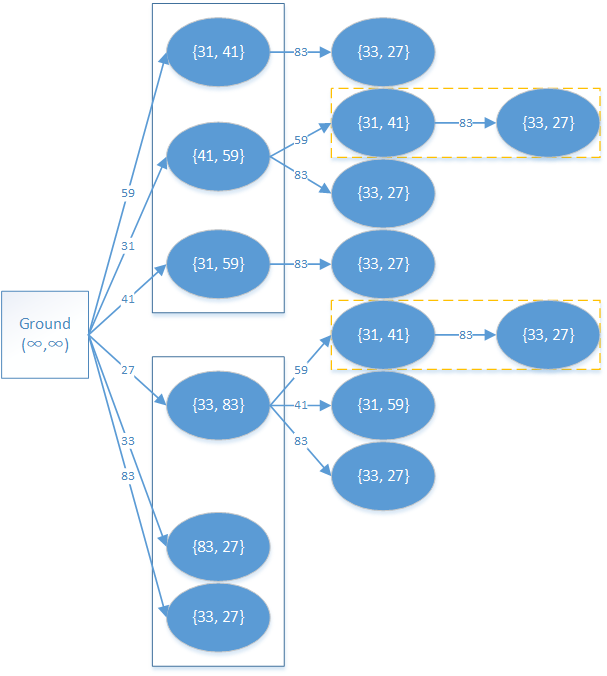
\includegraphics[width=0.7\textwidth]{docs/dp/images/dag-babylon.png} 

\end{figure}

图中蓝实框所表示的是一个砖块拆解得到的一组砖块,之所以用 $\{\}$ 表示底面边长,是因为砖块一旦选取了高,底面边长就是无序的。

图中黄虚框表示的是重复计算部分,为下文做铺垫。

\subsubsection{转移}

题目要求的是塔的最大高度,已经转化为最长路问题,其起点上文已指出是大地,那么终点呢?

显然终点已经自然确定,那就是某砖块上不能再搭别的砖块的时候。

之前在图上标记的黄虚框表明有重复计算,下面我们开始考虑转移方程。

显然,砖块一旦选取了高,那么这块砖块上最大能放的高度是确定的。

某个砖块 $i$ 有三种堆叠方式分别记为 $0, 1, 2$,那么对于砖块 $i$ 和其堆叠方式 $r$ 来说则有如下转移方程

$d(i, r) = \max\left\{d(j, r') + h'\right\}$

其中 $j$ 是所有那些在砖块 $i$ 以 $r$ 方式堆叠时可放上的砖块,$r'$ 对应 $j$ 此时的摆放方式,也就确定了此时唯一的高度 $h'$。

在实际编写时,将所有 $d(i, r)$ 都初始化为 $-1$,表示未计算过。

在试图计算前,如果发现已经计算过,直接返回保存的值;否则就按步计算,并保存。

最终答案是所有 $d(i, r)$ 的最大值。

\subsubsection{题解}

\begin{cppcode}
#include <cstring>
#include <iostream>
#define MAXN (30 + 5)
#define MAXV (500 + 5)
#define MAX(a, b) (((a) > (b)) ? (a) : (b))
int d[MAXN][3];
int x[MAXN], y[MAXN], z[MAXN];
int babylon_sub(int c, int rot, int n) {
  if (d[c][rot] != -1) {
    return d[c][rot];
  }
  d[c][rot] = 0;
  int base1, base2;
  if (rot == 0) {
    base1 = x[c];
    base2 = y[c];
  }
  if (rot == 1) {
    base1 = y[c];
    base2 = z[c];
  }
  if (rot == 2) {
    base1 = x[c];
    base2 = z[c];
  }
  for (int i = 0; i < n; i++) {
    if ((x[i] < base1 && y[i] < base2) || (y[i] < base1 && x[i] < base2))
      d[c][rot] = MAX(d[c][rot], babylon_sub(i, 0, n) + z[i]);
    if ((y[i] < base1 && z[i] < base2) || (z[i] < base1 && y[i] < base2))
      d[c][rot] = MAX(d[c][rot], babylon_sub(i, 1, n) + x[i]);
    if ((x[i] < base1 && z[i] < base2) || (z[i] < base1 && x[i] < base2))
      d[c][rot] = MAX(d[c][rot], babylon_sub(i, 2, n) + y[i]);
  }
  return d[c][rot];
}
int babylon(int n) {
  for (int i = 0; i < n; i++) {
    d[i][0] = -1;
    d[i][1] = -1;
    d[i][2] = -1;
  }
  int r = 0;
  for (int i = 0; i < n; i++) {
    r = MAX(r, babylon_sub(i, 0, n) + z[i]);
    r = MAX(r, babylon_sub(i, 1, n) + x[i]);
    r = MAX(r, babylon_sub(i, 2, n) + y[i]);
  }
  return r;
}
int main() {
  int t = 0;
  while (true) {
    int n;
    std::cin >> n;
    if (n == 0) break;
    t++;
    for (int i = 0; i < n; i++) {
      std::cin >> x[i] >> y[i] >> z[i];
    }
    std::cout << "Case " << t << ":"
              << " maximum height = " << babylon(n);
    std::cout << std::endl;
  }
  return 0;
}
\end{cppcode}

\section{树形 DP}

在学习本章前请确认你已经学习了 动态规划部分简介 

树形 DP,即在树上进行的 DP。由于树固有的递归性质,树形 DP 一般都是递归进行的。

\subsection{例题}

以下面这道题为例,介绍一下树形 DP 的一般过程。

\begin{NOTE}{例题 \href{https://www.luogu.org/problemnew/show/P1352}{洛谷 P1352 没有上司的舞会}}{}
某大学有 $n$ 个职员,编号为 $1\text{~} N$ 。他们之间有从属关系,也就是说他们的关系就像一棵以校长为根的树,父结点就是子结点的直接上司。现在有个周年庆宴会,宴会每邀请来一个职员都会增加一定的快乐指数 $a_i$,但是呢,如果某个职员的上司来参加舞会了,那么这个职员就无论如何也不肯来参加舞会了。所以,请你编程计算,邀请哪些职员可以使快乐指数最大,求最大的快乐指数。

\end{NOTE}


我们可以定义 $f(i,0/1)$ 代表以 $i$ 为根的子树的最优解(第二维的值为 0 代表 $i$ 不参加舞会的情况,1 代表 $i$ 参加舞会的情况)。

显然,我们可以推出下面两个状态转移方程(其中下面的 $x$ 都是 $i$ 的儿子):

\begin{itemize}
\item $f(i,0) = \sum\max \{f(x,1),f(x,0)\}$ (上司不参加舞会时,下属可以参加,也可以不参加)
\item $f(i,1) = \sum{f(x,0)} + a_i$ (上司参加舞会时,下属都不会参加)
\end{itemize}

我们可以通过 DFS,在返回上一层时更新当前节点的最优解。

代码:

\begin{cppcode}
#include <algorithm>
#include <cstdio>
using namespace std;
struct edge {
  int v, next;
} e[6005];
int head[6005], n, cnt, f[6005][2], ans, is_h[6005], vis[6005];
void addedge(int u, int v) {
  e[++cnt].v = v;
  e[cnt].next = head[u];
  head[u] = cnt;
}
void calc(int k) {
  vis[k] = 1;
  for (int i = head[k]; i; i = e[i].next)  //枚举该节点的每个子节点
  {
    if (vis[e[i].v]) continue;
    calc(e[i].v);
    f[k][1] += f[e[i].v][0];
    f[k][0] += max(f[e[i].v][0], f[e[i].v][1]);
  }
  return;
}
int main() {
  scanf("%d", &n);
  for (int i = 1; i <= n; i++) scanf("%d", &f[i][1]);
  for (int i = 1; i < n; i++) {
    int l, k;
    scanf("%d%d", &l, &k);
    is_h[l] = 1;
    addedge(k, l);
  }
  for (int i = 1; i <= n; i++)
    if (!is_h[i])  //从根节点开始DFS
    {
      calc(i);
      printf("%d", max(f[i][1], f[i][0]));
      return 0;
    }
}
\end{cppcode}

\subsection{习题}

\href{http://acm.hdu.edu.cn/showproblem.php?pid=2196}{HDU 2196 Computer}

\href{http://poj.org/problem?id=1463}{POJ 1463 Strategic game}

\href{http://poj.org/problem?id=3585}{POJ 3585 Accumulation Degree}

\section{状压 DP}

学习状压 dp 之前,请确认你已经完成了 动态规划初步 部分内容的学习

(建议学习 位运算 部分的内容)

\subsubsection{状压 dp 简介}

状压 dp 是动态规划的一种,借由将状态压缩(通常压缩为某整形)以达到节约空间和时间的目的

\paragraph{常用格式}

\begin{cppcode}
int maxn = 1 << n;  //规定状态的上界
for (int i = 0; i < maxn; i++) {
  if (i & (i << 1)) continue;  //如果i情况不成立就忽略
  Type[++top] = i;             //记录情况i到Type数组中
}
for (int i = 1; i <= top; i++) {
  if (fit(situation[1], Type[i])) dp[1][Type[i]] = 1;  //初始化第一层
}
for (int i = 2; i <= 层数(dp上界); i++) {
  for (int l = 1; l <= top; l++)  //穷举本层情况
    for (int j = 1; j <= top; j++)  //穷举上一层情况(上一层对本层有影响时)
      if (situation[i], Type[l] 和Type[j] 符合题意)
        dp[i][l] = dp[i][l] + dp[i - 1][j];  //改变当前层(i)的状态(l)的方案种数
}
for (int i = 1; i <= top; i++) ans += dp[上界][Type[i]];
\end{cppcode}

\paragraph{典型例题}

\href{https://www.luogu.org/problemnew/show/P1879}{玉米田 Corn Fields}

显然,这是一道典型的动态规划题目,但由于方案数过多,应使用状压 dp 避免超时

本题所 "压缩" 的是 "每行可行的状态" 和 "每行土地的状态", 而储存答案的 dp 数组就应同时体现这两个特点 (所以本题 dp 数组为二维)

具体实现方法同上方伪代码

\href{https://www.luogu.org/paste/kto3ua68}{例题代码}

\section{数位 DP}

\subsection{经典题型}

数位 DP 问题往往都是这样的题型,给定一个闭区间 $[l,r]$,让你求这个区间中满足 \textbf{某种条件} 的数的总数。

\begin{NOTE}{例题 \href{https://www.luogu.org/problemnew/show/P2657}{洛谷 P2657 windy 数}}{}
题目大意:给定一个区间 $[l,r]$ ,求其中满足条件 \textbf{不含前导 $0$ 且相邻两个数字相差至少为 $2$} 的数字个数。

\end{NOTE}


首先我们将问题转化成更加简单的形式。设 $ans_i$ 表示在区间 $[1,i]$ 中满足条件的数的数量,那么所求的答案就是 $ans_r-ans_{l-1}$。

分开求解这两个问题。

对于一个小于 $n$ 的数,它从高到低肯定出现某一位,使得这一位上的数值小于 $n$ 这一位上对应的数值。而之前的所有位都和 $n$ 上的位相等。

有了这个性质,我们可以定义 $f(i,st,op)$ 表示当前将要考虑的是从高到低的第 $i$ 位,当前该前缀的状态为 $st$ 且前缀和当前求解的数字的大小关系是 $op$ ($op=1$ 表示等于,$op=0$ 表示小于)时的数字个数。在本题中,这个前缀的状态就是上一位的值,因为当前将要确定的位不能取哪些数只和上一位有关。在其他题目中,这个值可以是:前缀的数字和,前缀所有数字的 $\gcd$,该前缀取模某个数的余数,也有两种或多种合用的情况。

写出 \textbf{状态转移方程} : $f(i,st,op)=\sum_{i=1}^{maxx} f(i+1,k,op=1~ \operatorname{and}~ i=maxx )\quad (|st-k|\ge 2)$

这里的 $k$ 就是当前枚举的下一位的值,而 $maxx$ 就是当前能取到的最高位。因为如果 $op=1$,那么你在这一位上取的值一定不能大于求解的数字上该位的值,否则则没有限制。

我们发现,尽管前缀所选择的状态不同,而 $f$ 的三个参数相同,答案就是一样的。为了防止这个答案被计算多次,可以使用记忆化搜索的方式实现。

核心代码:

\begin{cppcode}
int dfs(int x, int st, int op)  // op=1 =;op=0 <
{
  if (!x) return 1;
  if (!op && ~f[x][st]) return f[x][st];
  int maxx = op ? dim[x] : 9, ret = 0;
  for (int i = 0; i <= maxx; i++) {
    if (abs(st - i) < 2) continue;
    if (st == 11 && i == 0)
      ret += dfs(x - 1, 11, op & (i == maxx));
    else
      ret += dfs(x - 1, i, op & (i == maxx));
  }
  if (!op) f[x][st] = ret;
  return ret;
}
int solve(int x) {
  memset(f, -1, sizeof f);
  dim.clear();
  dim.push_back(-1);
  int t = x;
  while (x) {
    dim.push_back(x % 10);
    x /= 10;
  }
  return dfs(dim.size() - 1, 11, 1);
}
\end{cppcode}

\subsection{几道练习题}

\href{https://www.lydsy.com/JudgeOnline/problem.php?id=3679}{BZOJ 3679 数字之积 }

\href{https://www.luogu.org/problemnew/show/P2602}{洛谷 P2602 数字计数 }

\href{https://www.luogu.org/problemnew/show/P4127}{洛谷 P4127 同类分布 }

\href{https://www.luogu.org/problemnew/show/P3413}{洛谷  P3413 SAC - 萌数}

\href{http://acm.hdu.edu.cn/showproblem.php?pid=6148}{HDU 6148 Valley Number }

\href{http://codeforces.com/problemset/problem/55/D}{CF55D Beautiful numbers}

\href{http://codeforces.com/problemset/problem/628/D}{CF628D Magic Numbers}

\href{http://codeforces.com/problemset/problem/401/D}{CF401D Roman and Numbers}

\section{插头 DP}



\section{DP 优化}

本章主要讲解动态规划的几种基础 \textbf{ 优化 } 方法。

\subsection{二进制优化解多重背包}

\begin{NOTE}{例题  经典问题 - 多重背包}{}
题目大意:有 $n$ 种物品,每种物品有 $a_i$ 件,购买一件这种物品的费用为 $c_i$,价值为 $v_i$。有一个容量为 $t$ 的背包,现在让你找到最优的一种方案,使得装入背包的物品的总价值最大。

\end{NOTE}


考虑常规的动规方式,定义 $f_{i,j}$ 为当前考虑到第 $i$ 个物品,背包容量为 $j$ 所能获得的最大价值。

状态转移方程为, $f_{i,j}=\max\{f_{i-1,j},f_{i-1,j-c_i}+v_i\}$。

对于 \textbf{ 每件 } 物品,都要这样循环一次,时间复杂度为 $t\times \sum_{i=1}^n a_i$,某些时候可能不可接受,需要优化。

考虑这样一种情况,如果我们有 $17$ 个硬币,要去买 $1$ 到 $17$ 元钱的物品,只需将这些硬币打包成 $1,2,4,8$ 和 $2$ 这样的几包。前面的 $4$ 包能保证覆盖 $1$ 到 $15$ 所有的情况,最后一包在之前的基础上再加上一个值,能保证实现支付的时候取整包,肯定能保证支付。这就是二进制优化的原理和基本思想。

用上述的方法,就可以把 $k$ 件相同的物品看作是 $O(log_2 k)$ 件物品了。优化后

代码实现:

\begin{cppcode}
for (int i = 1; i <= n; i++) {
  scanf("%d", a + i);
  tot += c[i] * a[i];
  for (int j = 1; j <= a[i]; j *= 2)
    if (a[i] >= j) a[i] -= j, v[++cur] = c[i] * j;
  if (a[i]) v[++cur] = c[i] * a[i];
}
for (int i = 1; i <= cur; i++)
  for (int j = m; j >= v[i]; j--)
    if (f[j - v[i]]) f[j] = true;
\end{cppcode}

\subsection{几道练习题}

\href{http://acm.hdu.edu.cn/showproblem.php?pid=2844}{HDU 2844 Coins}

\subsection{单调队列 \& 单调栈优化}

学习本节前,请务必先学习  单调队列 。

\begin{NOTE}{例题 \href{http://codeforces.com/problemset/problem/372/C}{CF372C Watching Fireworks is Fun}}{}
题目大意:城镇中有 $n$ 个位置,有 $m$ 个烟花要放。第 $i$ 个烟花放出的时间记为 $t_i$,放出的位置记为 $a_i$。如果烟花放出的时候,你处在位置 $x$,那么你将收获 $b_i-|a_i-x|$ 点快乐值。
\end{NOTE}


初始你可在任意位置,你每个单位时间可以移动不大于 $d$ 个单位距离。现在你需要最大化你能获得的快乐值。

设 $f_{i,j}$ 表示在放第 $i$ 个烟花时,你的位置在 $j$ 所能获得的最大快乐值。

写出 \textbf{ 状态转移方程 } :$f_{i,j}=\max\{f_{i-1,k}+b_i-|a_i-j|\}$

这里的 $k$ 是有范围的,$j-(t_{i+1}-t_i)\times d\le k\le j+(t_{i+1}-t_i)\times d$。

我们尝试将状态转移方程进行变形:

由于 $\max$ 里出现了一个确定的常量 $b_i$,我们可以将它提到外面去。

$f_{i,j}=\max\{f_{i-1,k}+b_i+|a_i-j|\}=\max\{f_{i-1,k}-|a_i-j|\}+b_i$

如果确定了 $i$ 和 $j$ 的值,那么 $|a_i-j|$ 的值也是确定的,也可以将这一部分提到外面去。

最后,式子变成了这个样子:$f_{i,j}=\max\{f_{i-1,k}-|a_i-j|\}+b_i=\max\{f_{i-1,k}\}-|a_i-j|+b_i$

看到这一熟悉的形式,我们想到了什么?\textbf{ 单调队列优化 }。由于最终式子中的 $\max$ 只和上一状态中连续的一段的最大值有关,所以我们在计算一个新的 $i$ 的状态值时候只需将原来的 $f_{i-1}$ 构造成一个单调队列,并维护单调队列,使得其能在均摊 $O(1)$ 的时间复杂度内计算出 $\max\{f_{i-1,k}\}$ 的值,从而根据公式计算出 $f_{i,j}$ 的值。

总的时间复杂度为 $O(n\times m)$。

讲完了,让我们归纳一下单调队列优化动态规划问题的基本形态:当前状态的所有值可以从上一个状态的某个连续的段的值得到,要对这个连续的段进行 RMQ 操作,相邻状态的段的左右区间满足非降的关系。

\subsubsection{几道练习题}

\href{https://www.luogu.org/problemnew/show/P1886}{洛谷 P1886 滑动窗口}

\href{https://www.luogu.org/problemnew/show/P2254}{洛谷 P2254 瑰丽华尔兹}

\href{https://www.luogu.org/problemnew/show/P2569}{洛谷 P2569 股票交易}

\subsection{斜率优化}

\begin{NOTE}{例题 \href{https://www.luogu.org/problemnew/show/P3195}{洛谷 P3195 玩具装箱 TOY}}{}
令 $f_i$ 表示前 $i$ 个物品,随意分组装在任意多个容器里所能得到的最小费用。

\end{NOTE}


写出 \textbf{ 状态转移方程 } :$f_i=max\{f_j+(pre_i-pre_i+i-j-1-L)^2\}$ ,其中 $pre_i$ 表示前 $i$ 个数的前缀和。

换元试图简化状态转移方程式: 令 $s_i=pre_i+i,L'=L+1$,则 $f_i=f_j+(s_i-s_j-L')^2$,展开,移项得

$f_i=f_j+(s_i-s_j-L')^2$

$f_i+2\times s_i\times (s_j+L')=f_j+s_i^2+(s_j+L')^2$

我们观察到,式子的右端的所有项都只和 $i$ 有关或只和 $j$ 有关,式子左端的第一项是我们要求的目标值,式子左端的其余项都同时和 $i$ 和 $j$ 有关。我们将这个式子看作一条直线的函数解析式,形如 $b+k\times x=y$ ,和上式一一对应。我们发现如果我们要最小化 $f_i$ ,也就是说要最小化这个直线的截距,而对于每个确定的 $i$,这个直线的斜率 $s_i$ 都是确定的。

\begin{figure}[htbp]
\centering
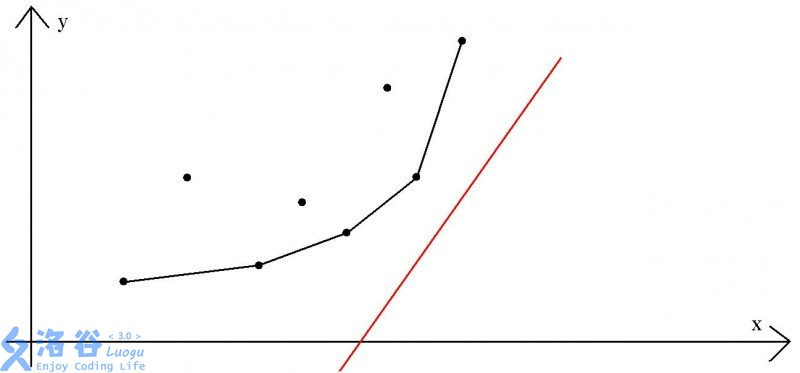
\includegraphics[width=0.7\textwidth]{docs/dp/images/optimization.png} 

\end{figure}

如图,我们将这个斜率固定的直线从下往上平移,直到有一个点在这条直线上,然后将新的点加入点集,这样肯定能保证所有的直线的斜率都是单调递升的(因为如果新的直线斜率小于斜率最大的直线,那么其一定不成被选择成为新的决策),所以我们相当于维护了一个下凸包。(如果求的是 $\max$ 那么就要维护一个 \textbf{ 上凸包 } 。这种东西要具体情况具体分析,如果直线的斜率不满足单调性,那就要维护整个凸包 / 二分等奇技淫巧。)

可以用单调队列维护下凸包。

\subsubsection{几道练习题}

\href{https://www.luogu.org/problemnew/show/P4072}{洛谷 P4072 征途}

\href{https://www.luogu.org/problemnew/show/P2120}{洛谷 P2120 仓库建设}

\href{https://www.luogu.org/problemnew/show/P3628}{洛谷 P3628 特别行动队}

\href{https://www.lydsy.com/JudgeOnline/problem.php?id=4709}{bzoj 4709 柠檬}

\href{http://codeforces.com/problemset/problem/311/B}{CF311B Cats Transport}

\href{https://www.luogu.org/problemnew/show/P4027}{洛谷 P4027 货币兑换}

\subsection{四边形不等式优化}

\begin{NOTE}{例题 \href{https://www.luogu.org/problemnew/show/P1880}{洛谷 P1880 石子合并}}{}
题目大意:在一个环上有 $n$ 个数,进行 $n-1$ 次合并操作,每次操作将相邻的两堆合并成一堆,能获得新的一堆中的石子数量的和的得分。你需要最大化你的得分。

\end{NOTE}


我们首先 \textbf{ 破环成链 } ,然后进行动态规划。设 $f_{i,j}$ 表示从位置 $i$ 合并到位置 $j$ 所能得到的最大得分, $sum_i$ 为前 $i$ 堆石子数的前缀和。

写出 \textbf{ 状态转移方程 } : $f_{i,j}=\max\{f_{i,k}+f_{k+1,j}+(sum_j-sum_i)\}(i\le k\le j)$

考虑常规的转移方法,枚举 $i$、$j$ 和 $k$,时间复杂度为 $O(n^3)$。

\subsubsection{什么是四边形不等式?}

对于 $a<b\le c<d$,如果有$f_{a,c}+f_{b,d}\le f_{b,c}+f_{a,d}$,则称该数组满足四边形不等式,可以用通俗的方法表述为 “交叉小于包含”。

两个定理:

\begin{enumerate}
\item 四边形不等式能优化的状态转移方程能表示为 $f_{i,j}=\max\{f_{i,k}+f_{k+1,j}+cost(i,j)\}(i\le k\le j)$。如果 $cost$ 函数同时满足单调性和四边形不等式,那么数组 $f$ 也满足四边形不等式。
\item 定义 $idx_{i,j}$ 为在转移 $f_{i,j}$ 的过程中在 $k=idx_{i,j}$ 时取得最小值,那么有如下定理:
如果 $f$ 数组满足四边形不等式,那么 $idx$ 函数满足单调性,即有 $idx_{i,j}\le idx_{i,j+1}\le idx_{i+1,j+1}$ 。
\end{enumerate}

证明会和题目解法一起 $qwq$ 

\subsubsection{回到题目}

第一步:证明 $cost$ 满足四边形不等式

要证明,对于所有满足 $i<i+1\le j<j+1$ 的 $i,j$ , 均有 $cost_{i,j}+cost_{i+1,j+1}\le cost_{i+1,j}+cost_{i,j+1}$。

移项得 $cost_{i,j}-cost_{i+1,j}\le cost_{i,j+1}-cost_{i+1,j+1}$

设 $F(j)=cost_{i,j}-cost{i+1,j}$ ,如果要使这个四边形不等式成立,那么就要证明 $F(j)$ 单调非降。

在本题中, $F(j)=(sum_j-sum_{i-1})-(sum_j-sum_i)=sum_i-sum_{i-1}=a_i$ ,与 $j$ 无关,自然一定满足四边形不等式。

证毕。

第二步:证明 $f$ 满足四边形不等式

同样的,应有如下结论:对于所有满足 $i<i+1\le j<j+1$ 的 $i,j$ , 均有 $f_{i,j}+f_{i+1,j+1}\le f_{i+1,j}+f_{i,j+1}$

我们假设 $x=idx_{i+1,j},y=idx_{i,j+1}$。不妨设 $x<=y$。

将 $x,y$ 带入得,$f_{i,j}+f_{i+1,j+1}=f_{i,x}+f_{x+1,j}+cost_{i,j}+f_{i+1,y}+f_{y+1,j+1}+cost_{i+1,j+1}$

由于上一步已经证明出了$cost$满足四边形不等式,而该不等式的左边在上式出现过,将其替换得

$$
\begin{aligned}
&&f_{i,\,x}+f_{x+1,\,j}+cost_{i,\,j}+f_{i+1,\,y}+f_{y+1,\,j+1}+cost_{i+1,\,j+1}\\
&\le&f_{i,\,x}+f_{x+1,\,j+1}+cost_{i,\,j+1}+f_{i+1,\,y}+f_{y+1,\,j}+cost_{i+1,\,j}\\
\end{aligned}
$$

消去公共项可得 $f_{i,j}+f_{i+1,j+1}\le f_{i+1,j}+f_{i,j+1}$

证毕。

第三步:证明决策的单调性

现在我们已经证明了 $cost$ 和 $f$ 满足四边形不等式,要证明决策的单调性以证明优化的正确性。

即证 $idx_{i,j-1}\le idx_{i,j}\le idx_{i+1,j}$

我们只证明式子的前半部分,后半部分可以有类似的方法推出。

设 $y=idx_{i,j-1},x\le y$ ,因为 $x+1\le y+1\le j-1<j$,由四边形不等式可得,

$f_{x+1,j-1}+f_{y+1,j}\le f_{y+1,j-1}+f_{x+1,j}$

由于我们是令 $y=idx_{i,j-1},x\le y$ 时 $f_{i,j-1}$ 取得最小值,那么 $f_{i,j-1}(idx_{i,j-1}=x)$ 一定大于等于 $f_{i,j-1}(idx_{i,j-1}=y)$ ,所以对于 $f_{i,j-1}$ 可以取到最优值的 $y$ ,所有小于它的值,对于 $f_{i,j}$ 来说,都没有 $y$ 优,所以最优决策一定不是小于 $y$ 的,那么一定有 

$idx_{i,j-1}\le idx_{i,j}$ 

证毕。

\subsubsection{说了这么多,怎么进行状态转移呢?}

给出核心代码:

\begin{cppcode}
for (int i = n; i >= 1; i--) {
  for (int j = i + 1; j <= n; j++) {
    f[i][j] = inf;
    for (int k = s[i][j - 1]; k <= s[i + 1][j]; k++) {
      if (f[i][j] < f[i][k] + f[k + 1][j] + sum[j] - sum[i - 1]) {
        f[i][j] = f[i][k] + f[k + 1][j] + sum[j] - sum[i - 1];
        idx[i][j] = k;
      }
    }
  }
}
\end{cppcode}

注意:由于在计算 $f_{i,j}$ 的时候需要知道 $idx_{i,j-1}$ 和 $idx_{i+1,j}$ 的值,所以 $i$ 的循环逆序。

\subsubsection{时间复杂度证明}

计算 $f_{i,j}$ 时,我们要循环 $idx_{i+1,j}-idx_{i,j-1}$ 次,那么一共加起来会循环多少次呢?

因为 $\sum_{i=1}^{n-1}(idx_{i+1,i+1}-idx_{i,i})=idx_{n,n}-idx_{1,1}$ 很显然和 $n$ 同阶,那么它的 $n$ 倍就和 $n^2$ 同阶,时间复杂度是 $O(n^2)$。

\subsubsection{一道练习题:}

\href{https://www.luogu.org/problemnew/show/P4767}{洛谷 P4767 邮局}

\subsubsection{参考资料}

\href{https://blog.csdn.net/noiau/article/details/72514812}{NOIAu 的 CSDN 博客}

\section{其它 DP 方法}



\chapter{字符串}
\section{字符串部分简介}

\subsection{字符串是啥?}

字符串可以看作是字符序列。

\subsection{字符集}

字符集是符号和文字组成的集合,在 OI 中,处理字符串时计算复杂度往往要考虑到字符集大小带来的常数影响。

举个栗子,如果一道题只包含'A' \textasciitilde{} 'Z' 意味着字符集大小是 26 。 如果再加上 '0' ~ '9' 字符集大小就变成了 36

计算复杂度时,字符集大小带来的常数往往要用 $\alpha$ 表示。

\subsection{如何存字符串}

可以开一个 \texttt{char} 数组 , 如 \texttt{char a[100]}

也可以用 \texttt{vector} 如  \texttt{vector<char> v}

同时 STL 中也提供了字符串容器 \texttt{std :: string} 

另外,在 \texttt{C / C++} 中也可以声明字符串字面量,比如 \texttt{char *buf = "XD"}。

\subsection{字符串存储的位置}

\begin{itemize}
\item 字符串字面量:它们的值在编译过程中已经确定,保存在可执行目标文件的 \texttt{.rodata} 段内。
调用 \texttt{objdump -s -j .rodata 文件名} 可以查看 \texttt{.rodata} 段的具体内容。
\item 字符数组、\texttt{vector}、\texttt{string}:局部变量保存在栈中,全局变量若初始化了保存在可执行目标文件的 \texttt{.data} 段内,若未初始化保存在 \texttt{.bss} 段。
\end{itemize}


\section{C / C++ 标准库中的字符串}

\subsection{C 标准库}

C 标准库是在对字符数组进行操作

\subsubsection{strlen}

\texttt{int strlen(const char *str)} :返回从 \texttt{str[0]} 开始直到 \texttt{'\textbackslash{}0'} 的字符数。注意,未开启 O2 优化时,该操作写在循环条件中复杂度是 $\Theta(N)$ 的。

\subsubsection{printf}

\texttt{printf("\%s", s)}:用 \texttt{\%s} 来输出一个字符串(字符数组)。

\subsubsection{scanf}

\texttt{scanf("\%s", s)}:用 \texttt{\%s} 来读入一个字符串(字符数组)。

\subsubsection{sscanf}

\texttt{sscanf(const char *\_\_source, const char *\_\_format, ...)}:从字符串\texttt{\_\_source}里读取变量,比如\texttt{sscanf(str,"\%d",\&a)}。

\subsubsection{sprintf}

\texttt{sprintf(char *\_\_stream, const char *\_\_format, ...)}:将\texttt{\_\_format}字符串里的内容输出到\texttt{\_\_stream}中,比如\texttt{sprintf(str,"\%d",i)}。

\subsubsection{strcmp}

\texttt{int strcmp(const char *str1, const char *str2)}:按照字典序比较 \texttt{str1 str2} 若 \texttt{str1} 字典序小返回负值, 一样返回 0 ,大返回正值 请注意,不要简单的认为只有 \texttt{0, 1, -1}  三种,在不同平台下的返回值都遵循正负,但并非都是 \texttt{0, 1, -1}

\subsubsection{strcpy}

\texttt{char *strcpy(char *str, const char *src)} : 把 \texttt{src} 中的字符复制到 \texttt{str} 中, \texttt{str} \texttt{src} 均为字符数组头指针, 返回值为 \texttt{str} 包含空终止符号 \texttt{'\textbackslash{}0'} 。

\subsubsection{strncpy}

\texttt{char *strncpy(char *str, const char *src, int cnt)} :复制至多 \texttt{cnt} 个字符到 \texttt{str} 中,若 \texttt{src} 终止而数量未达 \texttt{cnt} 则写入空字符到 \texttt{str} 直至写入总共 \texttt{cnt} 个字符。

\subsubsection{strcat}

\texttt{char *strcat(char *str1, const char *str2)} : 将 \texttt{str2} 接到 \texttt{str1} 的结尾,用 \texttt{*str2} 替换 \texttt{str1} 末尾的 \texttt{'\textbackslash{}0'}  返回 \texttt{str1} 。

\subsubsection{strstr}

\subsubsection{strchr}

\subsubsection{strrchr}

\subsection{C++ 标准库}

C++ 标准库是在对字符串对象进行操作,同时也提供对字符数组的兼容。

\subsubsection{std::string}

\begin{itemize}
\item 赋值运算符 \texttt{=} 右侧可以是 \texttt{const string / string / const char* / char*}。
\item 访问运算符 \texttt{[cur]} 返回 \texttt{cur} 位置的引用。
\item 访问函数 \texttt{data() / c\_str()} 返回一个\texttt{const char*} 指针, 内容与该 \texttt{string} 相同。
\item 容量函数 \texttt{size()} 返回字符串字符个数。
\item 还有一些其他的函数如 \texttt{find()} 找到并返回某字符位置。
\item \texttt{std :: string} 重载了比较逻辑运算符,复杂度是 $\Theta(N)$ 的。
\end{itemize}

\section{字符串匹配}

\subsection{字符串匹配问题}

字符串匹配问题分为好多类:

\subsubsection{单串匹配}

一个模式串 (pattern),一个待匹配串,找出前者在后者中的所有出现位置

\subsubsection{多串匹配}

多个模式串,一个待匹配串(多个待匹配串还用说,直接连起来)

直接当做单串匹配肯定是可以的,但是效率不够高

\subsubsection{匹配一个串的任意后缀}

\subsubsection{匹配多个串的任意后缀}

\subsection{暴力做法}

对于每个位置,尝试对模式串和待匹配串进行比对

(伪代码)

\begin{minted}{text}
match(char *a, char *b, int n, int m) {
  ans = new vector();
  for (i = 0; i < n - m + 1; i++) {
    for (j = 0; j < m; j++) {
      if (a[i + j] != b[j]) break;
    }
    if (j == m) ans.push_back(i);
  }
  return ans;
}
\end{minted}

时间复杂度分析:

最坏时间复杂度是 $O(nm)$ 的,

最好是 $O(n)$ 的。

如果字符集的大小大于 1 (有至少两个不同的字符),平均时间复杂度是 $O(n)$ 的。

\subsection{Hash 的方法}

参见  Hash 

\subsection{KMP 算法}

参见  KMP 

\section{哈希}

在介绍 Hash 算法之前,首先你需要了解关于  字符串匹配  的事情。

\subsection{Hash 的思想}

Hash 的核心思想在于,暴力算法中,单次比较的时间太长了,应当如何才能缩短一些呢?

如果要求每次只能比较 $O(1)$ 个字符,应该怎样操作呢?

是比较第一个?最后一个?随便选一个?求所有字符的和?

我们定义一个把 string 映射成 int 的函数 $f$,这个 $f$ 称为是 Hash 函数。

我们希望这个函数 $f$ 可以方便地帮我们判断两个字符串是否相等。

具体来说,我们希望在 Hash 函数值不一样的时候,两个字符串一定不一样。

另外,反过来不需要成立。我们把这种条件称为是单侧错误。

我们需要关注的是什么?

时间复杂度和 Hash 的准确率。

通常我们采用的是多项式 Hash 的方法,即 $\operatorname{f}(s) = \sum s[i] \times b^i \pmod M$

这里面的 $b$ 和 $M$ 需要选取得足够合适才行,以使得 Hash 的冲突尽量均匀。

如果 $b$ 和 $M$ 互质,在输入随机的情况下,这个 Hash 函数在 $[0,M)$ 上每个值概率相等

此时错误率为 $\frac1M$ (单次比较)

在输入不是随机的情况下,效果也很好。

\subsection{Hash 的实现}

伪代码:

\begin{minted}{text}
match_pre(int n) {
    exp[0] = 1;
    for (i = 1; i < n; i++) {
        exp[i] = exp[i - 1] * b % M;
    }
}

match(char *a, char *b, int n, int m) {
    // match 函数返回:长度为 m 的串 b 在长度为 n 的串 a 中的匹配位置
    // hash(a, m) 函数用来获得某个字符串前 m 个字符的部分的 hash 值
    ans = new vector();
    int ha = hash(a, m);
    int hb = hash(b, m);
    for (i = 0; i < n - m + 1; i++) {
        if ((ha - hb * exp[i]) % M == 0) {
            ans.push_back(i);
        }
        ha = (ha - a[i] * exp[i] + a[i + m] * exp[i + m]) % M;
    }
    return ans;
}
\end{minted}

通过上面这段代码,可以发现,每次直接计算 Hash 是 $O(串长)$ 的

\subsection{Hash 的分析与改进}

改进时间复杂度或者错误率

在上述例子中,时间复杂度已经是 $O(n+m)$

我们来分析错误率

由于 $n >> m$,要进行约 $n$ 次比较,每次错误率 $\frac1{M}$ ,那么总错误率是?

先补充一些随机数学的知识(非严格地)

现在考虑这 $n$ 次比较,如果看成独立的,总错误率 $1-(1-1/M)^n$

当 $M >> n$ 时,总错误率接近于$\frac{n}{M}$

当 $M = n$ 时,接近于 $1-\frac{1}{e} (≈0.63)$

如果不是独立的,最坏情况也就是全部加起来,等于 $\frac{n}{M}$

要改进错误率,可以增加 $M$

选取一个大的 $M$,或者两个互质的小的 $M$

时间复杂度不变,单次错误率平方

\subsection{Hash 的应用}

不只是字符串中,在其他情况也可以用。

假设有个程序要对 $10^{18}$ 大小的数组进行操作,保证只有 $10^6$ 个元素被访问到

由于存不下,我们在每次操作时,对下标取 Hash 值(比如,直接 $\bmod M$),然后在 $M$ 大小的数组内操作

如果冲突了怎么办?

方案 1:尝试找下一个位置,下下个位置(优点:速度快;缺点:删除麻烦)

方案 2:在数组的每个位置直接挂一个链表

\section{前缀函数与 KMP 算法}

\subsection{前缀函数定义}

给定一个长度为 $n$ 的字符串 $s$,其\textbf{前缀函数}被定义为一个长度为 $n$ 的数组 $\pi$。其中 $\pi[i]$ 为既是子串 $s[0\dots i]$ 的前缀同时也是该子串的后缀的最长真前缀(proper prefix)长度。一个字符串的真前缀是其前缀但不等于该字符串自身。根据定义,$\pi[0] = 0$。

前缀函数的定义可用数学语言描述如下:

$$
\pi[i] = \max_{k = 0 \dots i}\{k: s[0 \dots k - 1] = s[i - (k - 1) \dots i]\}
$$

举例来说,字符串 \texttt{abcabcd} 的前缀函数为 $[0, 0, 0, 1, 2, 3, 0]$,字符串 \texttt{aabaaab} 的前缀函数为 $[0, 1, 0, 1, 2, 2, 3]$。

\subsection{朴素算法}

一个直接按照定义计算前缀函数的算法如下:

\begin{cppcode}
vector<int> prefix_function(string s) {
  int n = (int)s.length();
  vector<int> pi(n);
  for (int i = 0; i < n; i++)
    for (int k = 0; k <= i; k++)
      if (s.substr(0, k) == s.substr(i - k + 1, k)) pi[i] = k;
  return pi;
}
\end{cppcode}

显见该算法的时间复杂度为 $O(n^3)$,具有很大的改进空间。

\subsection{高效算法}

该算法由 Knuth 和 Pratt 在 1977 年提出,同年 Morris 也独立的提出该算法。该算法被用作一个子串搜索算法的核心函数。

\subsubsection{第一个优化}

第一个重要的观察是相邻的前缀函数值至多增加 $1$。

实际上,如不然,即 $\pi[i + 1] > \pi[i] + 1$,考察长度为 $\pi[i + 1]$ 的 $s[0 \dots i + 1]$ 的后缀可引出矛盾。该后缀去掉最后一个字符后,我们得到一个长度为 $\pi[i + 1] - 1$ 的 $s[0 \dots i]$ 的后缀。该后缀比 $\pi[i]$ 描述的后缀更优,同其定义矛盾。

下述图例展示了这个矛盾。假定位于位置 $i$ 和 $i + 1$ 的既是后缀同时也是前缀的最长真后缀的长度分别为 $2$ 和 $4$。则字符串 $s_0 s_1 s_2 s_3$ 与字符串 $s_{i - 2} s_{i - 1} s_i s_{i + 1}$ 相同,这意味着 $s_0 s_1 s_2$ 与字符串 $s_{i - 2} s_{i - 1} s_i$ 相同,因此 $\pi[i]$ 至少为 $3$。

$$
\underbrace{\overbrace{s_0 ~ s_1}^{\pi[i] = 2} ~ s_2 ~ s_3}_{\pi[i+1] = 4} ~ \dots ~ \underbrace{s_{i-2} ~ \overbrace{s_{i-1} ~ s_{i}}^{\pi[i] = 2} ~ s_{i+1}}_{\pi[i+1] = 4}
$$

所以当移动到下一个位置时,前缀函数的值要么增加一,要么维持不变,要么减少。实际上,该事实已经允许我们将算法时间复杂度减少至 $O(n^2)$。因为每步中前缀函数至多增加 $1$,因此在总的运行过程中,前缀函数至多增加 $n$,同时也至多减小 $n$。这意味着我们仅需要进行 $O(n)$ 次字符串比较,所以总复杂度为 $O(n^2)$。

\subsubsection{第二个优化}

让我们走的更远一点:尝试摆脱掉字符串比较。为了达成这一点,我们必须用到先前计算的所有信息。

现在考虑计算位置 $i + 1$ 的前缀函数 $\pi$ 的值。如果 $s[i + 1] = s[\pi[i]]$,那么我们可以断言 $\pi[i + 1] = \pi[i] + 1$,因为我们已经知道位于位置 $i$ 的长度为 $\pi[i]$ 的后缀同长度为 $\pi[i]$ 的前缀相等。参照下述图例:

$$
\underbrace{\overbrace{s_0 ~ s_1 ~ s_2}^{\pi[i]} ~ \overbrace{s_3}^{s_3 = s_{i+1}}}_{\pi[i+1] = \pi[i] + 1} ~ \dots ~ \underbrace{\overbrace{s_{i-2} ~ s_{i-1} ~ s_{i}}^{\pi[i]} ~ \overbrace{s_{i+1}}^{s_3 = s_i + 1}}_{\pi[i+1] = \pi[i] + 1}
$$

如果不是上述情况,即 $s[i + 1] \neq s[\pi[i]]$,那么我们需要尝试更短的字符串。为了加速,我们希望直接移动到最长的长度 $j < \pi[i]$,使得在位置 $i$ 的前缀性质仍得以保持,也即 $s[0 \dots j - 1] = s[i - j + 1 \dots i]$:

$$
\overbrace{\underbrace{s_0 ~ s_1}_j ~ s_2 ~ s_3}^{\pi[i]} ~ \dots ~ \overbrace{s_{i-3} ~ s_{i-2} ~ \underbrace{s_{i-1} ~ s_{i}}_j}^{\pi[i]} ~ s_{i+1}
$$

实际上,如果我们找到了这样的长度 $j$,那么我们仅需要再次比较 $s[i + 1]$ 和 $s[j]$。如果他们相等,那么我们置 $\pi[i + 1] = j + 1$。否则,我们需要找到小于 $j$ 的最大值使得前缀性质得以保持,如此反复。这个过程会一直持续,直到 $j = 0$。如果 $s[i + 1] = s[0]$,那么我们置 $\pi[i + 1] = 1$,否则 $\pi[i + 1] = 0$。

所以我们已经有了这个算法的一个大概雏形。现在仅剩的问题是对于 $j$,如何快速找到这样的长度。让我们重新叙述一遍:对于当前在位置 $i$ 使得前缀性质得以保持的长度 $j$,也即 $s[0 \dots j - 1] = s[i - j + 1 \dots i]$,我们希望找到最大的 $k < j$,使得前缀性质仍得以保持。

$$
\overbrace{\underbrace{s_0 ~ s_1}_k ~ s_2 ~ s_3}^j ~ \dots ~ \overbrace{s_{i-3} ~ s_{i-2} ~ \underbrace{s_{i-1} ~ s_{i}}_k}^j ~s_{i+1}
$$

上图显示出 $k$ 必定为 $\pi[j - 1]$,而该值我们之前已经计算过了。

\subsubsection{最终算法}

所以最终我们可以构建一个不需要进行任何字符串比较,并且只进行 $O(n)$ 次操作的算法。

以下是最终的流程:

\begin{itemize}
\item 在一个循环中以 $i = 1$ 到 $i = n - 1$ 的顺序计算前缀函数 $\pi[i]$ 的值($\pi[0]$ 被赋值为 $0$)。
\item 为了计算当前的前缀函数值 $\pi[i]$,我们令变量 $j$ 表示右端点位于 $i - 1$ 的最好的后缀的长度。初始时 $j = \pi[i - 1]$。
\item 通过比较 $s[j]$ 和 $s[i]$ 来检查长度为 $j + 1$ 的后缀是否同时也是一个前缀。如果二者相等,那么我们置 $\pi[i] = j + 1$,否则我们减少 $j$ 至 $\pi[j - 1]$ 并且重复该过程。
\item 如果 $j = 0$ 并且仍没有任何一次匹配,则置 $\pi[i] = 0$ 并移至下一个下标 $i + 1$。
\end{itemize}

\subsubsection{实现}

该算法的实现出人意料的短且直观。

\begin{cppcode}
vector<int> prefix_function(string s) {
  int n = (int)s.length();
  vector<int> pi(n);
  for (int i = 1; i < n; i++) {
    int j = pi[i - 1];
    while (j > 0 && s[i] != s[j]) j = pi[j - 1];
    if (s[i] == s[j]) j++;
    pi[i] = j;
  }
  return pi;
}
\end{cppcode}

这是一个\textbf{在线}算法,即其当数据到达时处理它——举例来说,你可以一个字符一个字符的读取字符串,立即处理它们以计算出每个字符的前缀函数值。该算法仍然需要存储字符串本身以及先前计算过的前缀函数值,但如果我们已经预先知道该字符串前缀函数的最大可能取值 $M$,那么我们仅需要存储该字符串的前 $M + 1$ 个字符以及对应的前缀函数值。

\subsection{应用}

\subsubsection{在字符串中查找子串:Knuth-Morris-Pratt 算法}

该任务是前缀函数的一个典型应用。

给定一个文本 $t$ 和一个字符串 $s$,我们尝试找到并展示 $s$ 在 $t$ 中的所有出现(occurrence)。

为了简便起见,我们用 $n$ 表示字符串 $s$ 的长度,用 $m$ 表示文本 $t$ 的长度。

我们构造一个字符串 $s + \# + t$,其中 $\#$ 为一个既不出现在 $s$ 中也不出现在 $t$ 中的分隔符。接下来计算该字符串的前缀函数。现在考虑该前缀函数除去最开始 $n + 1$ 个值(即属于字符串 $s$ 和分隔符的函数值)后其余函数值的意义。根据定义,$\pi[i]$ 为右端点在 $i$ 且同时为一个前缀的最长真子串的长度,具体到我们的这种情况下,其值为与 $s$ 的前缀相同且右端点位于 $i$ 的最长子串的长度。由于分隔符的存在,该长度不可能超过 $n$。而如果等式 $\pi[i] = n$ 成立,则意味着 $s$ 完整出现在该位置(即其右端点位于位置 $i$)。注意该位置的下标是对字符串 $s + \# + t$ 而言的。

因此如果在某一位置 $i$ 有 $\pi[i] = n$ 成立,则字符串 $s$ 在字符串 $t$ 的 $i - (n - 1) - (n + 1) = i - 2n$ 处出现。

正如在前缀函数的计算中已经提到的那样,如果我们知道前缀函数的值永远不超过一特定值,那么我们不需要存储整个字符串以及整个前缀函数,而只需要二者开头的一部分。在我们这种情况下这意味着只需要存储字符串 $s + \#$ 以及相应的前缀函数值即可。我们可以一次读入字符串 $t$ 的一个字符并计算当前位置的前缀函数值。

因此 Knuth-Morris-Pratt 算法(简称 KMP 算法)用 $O(n + m)$ 的时间以及 $O(n)$ 的内存解决了该问题。

\subsubsection{统计每个前缀的出现次数}

在该节我们将同时讨论两个问题。给定一个长度为 $n$ 的字符串 $s$,在问题的第一个变种中我们希望统计每个前缀 $s[0 \dots i]$ 在同一个字符串的出现次数,在问题的第二个变种中我们希望统计每个前缀 $s[0 \dots i]$ 在另一个给定字符串 $t$ 中的出现次数。

首先让我们来解决第一个问题。考虑位置 $i$ 的前缀函数值 $\pi[i]$。根据定义,其意味着字符串 $s$ 一个长度为 $\pi[i]$ 的前缀在位置 $i$ 出现并以 $i$ 为右端点,同时不存在一个更长的前缀满足前述定义。与此同时,更短的前缀可能以该位置为右端点。容易看出,我们遇到了在计算前缀函数时已经回答过的问题:给定一个长度为 $j$ 的前缀,同时其也是一个右端点位于 $i$ 的后缀,下一个更小的前缀长度 $k < j$ 是多少?该长度的前缀需同时也是一个右端点为 $i$ 的后缀。因此以位置 $i$ 为右端点,有长度为 $\pi[i]$ 的前缀,有长度为 $\pi[\pi[i] - 1]$ 的前缀,有长度为 $\pi[\pi[\pi[i] - 1] - 1]$ 的前缀,等等,直到长度变为 $0$。故而我们可以通过下述方式计算答案。

\begin{cppcode}
vector<int> ans(n + 1);
for (int i = 0; i < n; i++) ans[pi[i]]++;
for (int i = n - 1; i > 0; i--) ans[pi[i - 1]] += ans[i];
for (int i = 0; i <= n; i++) ans[i]++;
\end{cppcode}

在上述代码中我们首先统计每个前缀函数值在数组 $\pi$ 中出现了多少次,然后再计算最后答案:如果我们知道长度为 $i$ 的前缀出现了恰好 $\text{ans}[i]$ 次,那么该值必须被叠加至其最长的既是后缀也是前缀的子串的出现次数中。在最后,为了统计原始的前缀,我们对每个结果加 $1$。

现在考虑第二个问题。我们应用来自 Knuth-Morris-Pratt 的技巧:构造一个字符串 $s + \# + t$ 并计算其前缀函数。与第一个问题唯一的不同之处在于,我们只关心与字符串 $t$ 相关的前缀函数值,即 $i \ge n + 1$ 的 $\pi[i]$。有了这些值之后,我们可以同样应用在第一个问题中的算法来解决该问题。

\subsubsection{一个字符串中本质不同子串的数目}

给定一个长度为 $n$ 的字符串 $s$,我们希望计算其本质不同子串的数目。

我们将迭代的解决该问题。换句话说,在知道了当前的本质不同子串的数目的情况下,我们要找出一种在 $s$ 末尾添加一个字符后重新计算该数目的方法。

令 $k$ 为当前 $s$ 的本质不同子串数量。我们添加一个新的字符 $c$ 至 $s$。显然,会有一些新的子串以字符 $c$ 结尾。我们希望对这些以该字符结尾且我们之前未曾遇到的子串计数。

构造字符串 $t = s + c$ 并将其反转得到字符串 $t^{\sim}$。现在我们的任务变为计算有多少 $t^{\sim}$ 的前缀未在 $t^{\sim}$ 的其余任何地方出现。如果我们计算了 $t^{\sim}$ 的前缀函数最大值 $\pi_{\max}$,那么最长的出现在 $s$ 中的前缀其长度为 $\pi_{\max}$。自然的,所有更短的前缀也出现了。

因此,当添加了一个新字符后新出现的子串数目为 $|s| + 1 - \pi_{\max}$。

所以对于每个添加的字符,我们可以在 $O(n)$ 的时间内计算新子串的数目,故最终复杂度为 $O(n^2)$。

值得注意的是,我们也可以重新计算在头部添加一个字符,或者从尾或者头移除一个字符时的本质不同子串数目。

\subsubsection{字符串压缩}

给定一个长度为 $n$ 的字符串 $s$,我们希望找到其最短的 “压缩” 表示,也即我们希望寻找一个最短的字符串 $t$,使得 $s$ 可以被 $t$ 的一份或多份拷贝的拼接表示。

显然,我们只需要找到 $t$ 的长度即可。知道了该长度,该问题的答案即为长度为该值的 $s$ 的前缀。

让我们计算 $s$ 的前缀函数。通过使用该函数的最后一个值 $\pi[n - 1]$,我们定义值 $k = n - \pi[n - 1]$。我们将证明,如果 $k$ 整除 $n$,那么 $k$ 就是答案,否则不存在一个有效的压缩,故答案为 $n$。

假定 $n$ 可被 $k$ 整除。那么字符串可被划分为长度为 $k$ 的若干块。根据前缀函数的定义,该字符串长度为 $n - k$ 的前缀等于其后缀。但是这意味着最后一个块同倒数第二个块相等,并且倒数第二个块同倒数第三个块相等,等等。作为其结果,所有块都是相等的,因此我们可以将字符串 $s$ 压缩至长度 $k$。

诚然,我们仍需证明该值为最优解。实际上,如果有一个比 $k$ 更小的压缩表示,那么前缀函数的最后一个值 $\pi[n - 1]$ 必定比 $n - k$ 要大。因此 $k$ 就是答案。

现在假设 $n$ 不可以被 $k$ 整除,我们将通过反证法证明这意味着答案为 $n$ \footnote{在俄文版及英文版中该部分证明均疑似有误。本文章中的该部分证明由作者自行添加。}。假设其最小压缩表示 $r$ 的长度为 $p$($p$ 整除 $n$),字符串 $s$ 被划分为 $n / p \ge 2$ 块。那么前缀函数的最后一个值 $\pi[n - 1]$ 必定大于 $n - p$(如果等于则 $n$ 可被 $k$ 整除),也即其所表示的后缀将部分的覆盖第一个块。现在考虑字符串的第二个块。该块有两种解释:第一种为 $r_0 r_1 \dots r_{p - 1}$,另一种为 $r_{p - k} r_{p - k + 1} \dots r_{p - 1} r_0 r_1 \dots r_{p - k - 1}$ 。由于两种解释对应同一个字符串,因此可得到 $p$ 个方程组成的方程组,该方程组可简写为 $r_{(i + k) \bmod p} = r_{i \bmod p}$,其中 $\cdot \bmod p$ 表示模 $p$ 意义下的最小非负剩余。

$$
\begin{gathered}
\overbrace{r_0 ~ r_1 ~ r_2 ~ r_3 ~ r_4 ~ r_5}^p ~ \overbrace{r_0 ~ r_1 ~ r_2 ~ r_3 ~ r_4 r_5}^p \\
r_0 ~ r_1 ~ r_2 ~ r_3 ~ \underbrace{\overbrace{r_0 ~ r_1 ~ r_2 ~ r_3 ~ r_4 ~ r_5}^p ~ r_0 ~ r_1}_{\pi[11] = 8}
\end{gathered}
$$

根据扩展欧几里得算法我们可以得到一组 $x$ 和 $y$ 使得 $xk + yp = \gcd(k, p)$。通过与等式 $pk - kp = 0$ 适当叠加我们可以得到一组 $x' > 0$ 和 $y' < 0$ 使得 $x'k + y'p = \gcd(k, p)$。这意味着通过不断应用前述方程组中的方程我们可以得到新的方程组 $r_{(i + \gcd(k, p)) \bmod p} = r_{i \bmod p}$。

由于 $\gcd(k, p)$ 整除 $p$,这意味着 $\gcd(k, p)$ 是 $r$ 的一个周期。又因为 $\pi[n - 1] > n - p$,故有 $n - \pi[n - 1] = k < p$,所以 $\gcd(k, p)$ 是一个比 $p$ 更小的 $r$ 的周期。因此字符串 $s$ 有一个长度为 $\gcd(k, p) < p$ 的压缩表示,同 $p$ 的最小性矛盾。

综上所述,不存在一个长度小于 $n$ 的压缩表示,因此答案为 $n$。

\subsubsection{根据前缀函数构建一个自动机}

让我们重新回到通过一个分隔符将两个字符串拼接的新字符串。对于字符串 $s$ 和 $t$ 我们计算 $s + \# + t$ 的前缀函数。显然,因为 $\#$ 是一个分隔符,前缀函数值永远不会超过 $|s|$。因此我们只需要存储字符串 $s + \#$ 和其对应的前缀函数值,之后就可以动态计算对于之后所有字符的前缀函数值:

$$
\underbrace{s_0 ~ s_1 ~ \dots ~ s_{n-1} ~ \#}_{\text{need to store}} ~ \underbrace{t_0 ~ t_1 ~ \dots ~ t_{m-1}}_{\text{do not need to store}}
$$

实际上在这种情况下,知道 $t$ 的下一个字符 $c$ 以及之前位置的前缀函数值便足以计算下一个位置的前缀函数值,而不需要用到任何其它 $t$ 的字符和对应的前缀函数值。

换句话说,我们可以构造一个\textbf{自动机}(一个有限状态机):其状态为当前的前缀函数值,而从一个状态到另一个状态的转移则由下一个字符确定。

因此,即使没有字符串 $t$,我们同样可以应用构造转移表的算法构造一个转移表 $( \text { old } \pi , c ) \rightarrow \text { new } _ { - } \pi$:

\begin{cppcode}
void compute_automaton(string s, vector<vector<int>>& aut) {
  s += '#';
  int n = s.size();
  vector<int> pi = prefix_function(s);
  aut.assign(n, vector<int>(26));
  for (int i = 0; i < n; i++) {
    for (int c = 0; c < 26; c++) {
      int j = i;
      while (j > 0 && 'a' + c != s[j]) j = pi[j - 1];
      if ('a' + c == s[j]) j++;
      aut[i][c] = j;
    }
  }
}
\end{cppcode}

然而在这种形式下,对于小写字母表,算法的时间复杂度为 $O(n^2 26)$。注意到我们可以应用动态规划来利用表中已计算过的部分。只要我们从值 $j$ 变化到 $\pi[j - 1]$,那么我们实际上在说转移 $(j, c)$ 所到达的状态同转移 $(\pi[j - 1], c)$ 一样,但该答案我们之前已经精确计算过了。

\begin{cppcode}
void compute_automaton(string s, vector<vector<int>>& aut) {
  s += '#';
  int n = s.size();
  vector<int> pi = prefix_function(s);
  aut.assign(n, vector<int>(26));
  for (int i = 0; i < n; i++) {
    for (int c = 0; c < 26; c++) {
      if (i > 0 && 'a' + c != s[i])
        aut[i][c] = aut[pi[i - 1]][c];
      else
        aut[i][c] = i + ('a' + c == s[i]);
    }
  }
}
\end{cppcode}

最终我们可在 $O(n 26)$ 的时间复杂度内构造该自动机。

该自动机在什么时候有用呢?首先,记得大部分时候我们为了一个目的使用字符串 $s + \# + t$ 的前缀函数:寻找字符串 $s$ 在字符串 $t$ 中的所有出现。

因此使用该自动机的最直接的好处是\textbf{加速计算字符串 $s + \# + t$ 的前缀函数}。

通过构建 $s + \#$ 的自动机,我们不再需要存储字符串 $s$ 以及其对应的前缀函数值。所有转移已经在表中计算过了。

但除此以外,还有第二个不那么直接的应用。我们可以在字符串 $t$ 是\textbf{某些通过一些规则构造的巨型字符串}时,使用该自动机加速计算。Gray 字符串,或者一个由一些短的输入串的递归组合所构造的字符串都是这种例子。

出于完整性考虑,我们来解决这样一个问题:给定一个数 $k \le 10^5$,以及一个长度 $\le 10^5$ 的字符串 $s$,我们需要计算 $s$ 在第 $k$ 个 Gray 字符串中的出现次数。回想起 Gray 字符串以下述方式定义:

$$
\begin{aligned}
g_1 &= \mathtt{a}\\
g_2 &= \mathtt{aba}\\
g_3 &= \mathtt{abacaba}\\
g_4 &= \mathtt{abacabadabacaba}
\end{aligned}
$$

由于其天文数字般的长度,在这种情况下即使构造字符串 $t$ 都是不可能的:第 $k$ 个 Gray 字符串有 $2^k - 1$ 个字符。然而我们可以在仅仅知道开头若干前缀函数值的情况下,有效计算该字符串末尾的前缀函数值。

除了自动机之外,我们同时需要计算值 $G[i][j]$:在从状态 $j$ 开始处理 $g_i$ 后的自动机的状态,以及值 $K[i][j]$:当从状态 $j$ 开始处理 $g_i$ 后,$s$ 在 $g_i$ 中的出现次数。实际上 $K[i][j]$ 为在执行操作时前缀函数取值为 $|s|$ 的次数。易得问题的答案为 $K[k][0]$。

我们该如何计算这些值呢?首先根据定义,初始条件为 $G[0][j] = j$ 以及 $K[0][j] = 0$。之后所有值可以通过先前的值以及使用自动机计算得到。为了对某个 $i$ 计算相应值,回想起字符串 $g_i$ 由 $g_{i - 1}$,字母表中第 $i$ 个字符,以及 $g_{i - 1}$ 三者拼接而成。因此自动机会途径下列状态:

$$
\begin{gathered}
\text{mid} = \text{aut}[G[i - 1][j]][i] \\
G[i][j] = G[i - 1][\text{mid}]
\end{gathered}
$$

$K[i][j]$ 的值同样可被简单计算。

$$
K[i][j] = K[i - 1][j] + [\text{mid} == |s|] + K[i - 1][\text{mid}]
$$

其中 $[\cdot]$ 当其中表达式取值为真时值为 $1$,否则为 $0$。综上,我们已经可以解决关于 Gray 字符串的问题,以及一大类与之类似的问题。举例来说,应用同样的方法可以解决下列问题:给定一个字符串 $s$ 以及一些模式 $t_i$,其中每个模式以下列方式给出:该模式由普通字符组成,当中可能以 $t_{k}^{\text{cnt}}$ 的形式递归插入先前的字符串,也即在该位置我们必须插入字符串 $t_k$ $\text{cnt}$ 次。以下是这些模式的一个例子:

$$
\begin{aligned}
t_1 &= \mathtt{abdeca} \\
t_2 &= \mathtt{abc} + t_1^{30} + \mathtt{abd} \\
t_3 &= t_2^{50} + t_1^{100} \\
t_4 &= t_2^{10} + t_3^{100}
\end{aligned}
$$

递归代入会使字符串长度爆炸式增长,他们的长度甚至可以达到 $100^{100}$ 的数量级。而我们必须找到字符串 $s$ 在每个字符串中的出现次数。

该问题同样可通过构造前缀函数的自动机解决。同之前一样,我们利用先前计算过的结果对每个模式计算其转移然后相应统计答案即可。

\subsection{练习题目}

\begin{itemize}
\item \href{http://uva.onlinejudge.org/index.php?option=onlinejudge&page=show_problem&problem=396}{UVA \textbackslash{}\# 455 "Periodic Strings"}
\item \href{http://uva.onlinejudge.org/index.php?option=onlinejudge&page=show_problem&problem=1963}{UVA \textbackslash{}\# 11022 "String Factoring"}
\item \href{http://uva.onlinejudge.org/index.php?option=onlinejudge&page=show_problem&problem=2447}{UVA \textbackslash{}\# 11452 "Dancing the Cheeky-Cheeky"}
\item \href{https://uva.onlinejudge.org/index.php?option=com_onlinejudge&Itemid=8&page=show_problem&problem=4282}{UVA 12604 - Caesar Cipher}
\item \href{https://uva.onlinejudge.org/index.php?option=com_onlinejudge&Itemid=8&page=show_problem&problem=3911}{UVA 12467 - Secret Word}
\item \href{https://uva.onlinejudge.org/index.php?option=onlinejudge&page=show_problem&problem=1960}{UVA 11019 - Matrix Matcher}
\item \href{http://www.spoj.com/problems/NAJPF/}{SPOJ - Pattern Find}
\item \href{http://codeforces.com/contest/808/problem/G}{Codeforces - Anthem of Berland}
\item \href{http://codeforces.com/problemset/problem/471/D}{Codeforces - MUH and Cube Walls}
\end{itemize}

\hr

\textbf{本页面主要译自博文 \href{http://e-maxx.ru/algo/prefix_function}{Префикс-функция. Алгоритм Кнута-Морриса-Пратта} 与其英文翻译版 \href{https://cp-algorithms.com/string/prefix-function.html}{Prefix function. Knuth–Morris–Pratt algorithm} 。其中俄文版版权协议为 Public Domain + Leave a Link;英文版版权协议为 CC-BY-SA 4.0。}

\section{字典树 (Trie)}

\subsection{Trie}

先考虑怎么存多个串

一种树,每个结点有 $|∑|$ 个儿子,每条边表示一个字符

空间 $O(len)$ (如果假设 $|∑|$ 为常数)

要判断某个串是否等于某个模式串,只要在 Trie 上走一遍(线性的)

\subsection{在 Trie 上 KMP}

实际上要做的事情是求出 Trie 的每个节点的 $next$ 值

当然,这里的 $next$ 不再是一个值,而是相当于是一个指针 —— 它可能指向其他分支的节点。

这时 $next$ 的定义:最长的等于同长度的后缀的从根开始的路径的长度

求法跟  KMP  中的一样,只是要改成在 Trie 上  BFS 

复杂度:均摊分析失效了,其实只能在每条链上均摊分析,于是总复杂度为模式串长总和

\section{回文自动机}



\section{回文树}



\section{后缀数组 (SA)}

\subsection{1. 前言}

\subsubsection{后缀数组和后缀树}

\begin{QUOTE}{}{}
在字符串处理当中,后缀树和后缀数组都是非常有力的工具。其实后缀数组是后缀树的一个非常精巧的替代品,它比后缀树容易编程实现,能够实现后缀树的很多功能而时间复杂度也不太逊色,并且,它比后缀树所占用的空间小很多。可以说,在信息学竞赛中后缀数组比后缀树要更为实用。——百度百科
\end{QUOTE}

\subsubsection{各种定义}

\texttt{子串}: 就是子串 [捂脸]

\texttt{后缀}: 就是从 $i$ 这个位置开始到该字符串的末尾的一个子串

\texttt{字符串大小}: $a$ 和 $b$ 这两个串,从头开始逐个字符按照 ASSIC 码进行比较

\texttt{后缀数组}: $sa[i]$ 代表该字符串的 $len$ 个后缀中,排名为 $i$ 的后缀是第 $sa[i]$ 个后缀

\texttt{名词数组}: $rank[i]$ 代表第 $i$ 个后缀排名为 $rank[i]$

\subsection{2. 一些构造方法}

\subsubsection{最简单的暴力}

把所有的后缀拆出来,然后 sort

思想较为简单,可自行尝试实现

\begin{cppcode}
#include <bits/stdc++.h>
using namespace std;

int rank[123], sa[123];

struct Str {
  string s;
  int wei;
  friend bool operator<(Str a1, Str a2) { return a1.s < a2.s; }
} k[123];

int main() {
  string s;
  cin >> s;
  int len = s.size() - 1;

  for (int i = 0; i <= len; i++) {
    k[i].wei = i;
    for (int j = i; j <= len; j++) k[i].s = k[i].s + s[j];
  }

  sort(k, k + len + 1);
  for (int i = 0; i <= len; i++) {
    rank[k[i].wei] = i;
    sa[i] = k[i].wei;
  }

  exit(0);
}
\end{cppcode}

\subsubsection{倍增}

这个就是一般人写后缀数组用的方法

复杂度是 $O(nlogn)$ 

前提是你要先会 \textbf{ 基数排序 }

假设我们有这样一个字符串 \texttt{aabaaaab}

然后我们把所有的后缀列举出来:

\begin{figure}[htbp]
\centering
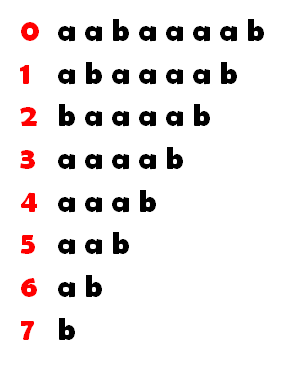
\includegraphics[width=0.7\textwidth]{docs/string/images/sa1.png} 

\end{figure}

然后用基数排序的方式,按照每个后缀的第一个字母进行排序,呈现这样子的效果:

\begin{figure}[htbp]
\centering
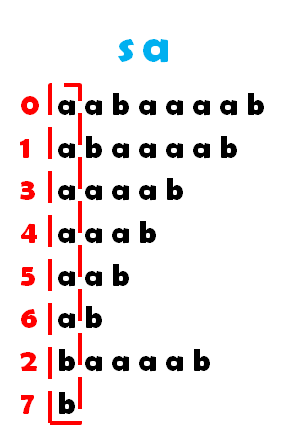
\includegraphics[width=0.7\textwidth]{docs/string/images/sa2.png} 

\end{figure}

接着我们以第二个字母为关键字,在首字母有序的基础上进行排序,这个时候,我们把首字母相同的后缀拿出来单看

对于每一组首字母相同的后缀,首字母是对排序没有影响的,所以可以直接按照第二个字母进行基数排序,同样,对于首字母不同的后缀,由于按照首字母排序时,他们的相对大小已经确定,当按照第二个字母排序时,不会出现 \texttt{原来 a>b,现在 b>a} 的现象,所以我们可以看成一直在做区域内的排序,这之后变成这样:

\begin{figure}[htbp]
\centering
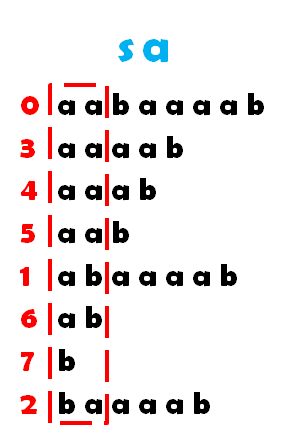
\includegraphics[width=0.7\textwidth]{docs/string/images/sa3.png} 

\end{figure}

第三字母同理........

这样子我们可以处理这个问题,可是复杂度还是没有到达一个我们可以接受的范围

所以我们引入 \textbf{ 倍增 }

当我们按照每个后缀的前 $2^k$ 个字母进行完排序后,那么我们把后缀的前 $2^{k+1}$ 看做前后两个 $2^k$, 这样我们就可以把这前后两个 $2^k$ 作为之前说的 \texttt{首字母} 和 \texttt{第二个字母} 了,然后进行上述过程,就可以在 $O(nlogn)$ 的复杂度内处理这个问题了

\begin{cppcode}
#include <bits/stdc++.h>
using namespace std;

int n;
int sa[150], x[150], c[150], y[150];
char a[150];

inline void SA() {
  int m = 128;
  for (int i = 0; i <= m; i++) c[i] = 0;
  for (int i = 1; i <= n; i++) c[x[i]]++;
  for (int i = 1; i <= m; i++) c[i] += c[i - 1];
  for (int i = n; i; i--) sa[c[x[i]]--] = i;

  for (int k = 1, p; k <= n; k <<= 1) {
    p = 0;
    for (int i = n; i > n - k; i--) y[++p] = i;
    for (int i = 1; i <= n; i++)
      if (sa[i] > k) y[++p] = sa[i] - k;

    for (int i = 0; i <= m; i++) c[i] = 0;
    for (int i = 1; i <= n; i++) c[x[i]]++;
    for (int i = 1; i <= m; i++) c[i] += c[i - 1];
    for (int i = n; i; i--) sa[c[x[y[i]]]--] = y[i];

    p = y[sa[1]] = 1;
    for (int i = 2, a, b; i <= n; i++) {
      a = sa[i] + k > n ? -1 : x[sa[i] + k];
      b = sa[i - 1] + k > n ? -1 : x[sa[i - 1] + k];
      y[sa[i]] = (x[sa[i]] == x[sa[i - 1]]) && (a == b) ? p : ++p;
    }
    swap(x, y);
    m = p;
  }
}

int main() {
  scanf("%s", a + 1);

  n = strlen(a + 1);
  for (int i = 1; i <= n; i++) x[i] = a[i];
  SA();

  for (int i = 1; i <= n; i++) printf("%d", sa[i]);
  exit(0);
}
\end{cppcode}

代码里 $x[i]$ 就是 $rank[i]$ 

$y[i]$ :假设 $y[i]=a\ ,\  y[i+1]=b$ 那么在原串中 从 $a+2^k$ 开始的 $2^k$ 个字符组成的子串 \textbf{ 小于等于 } 从 $b+2^k$ 开始的 $2^k$ 个字符组成的子串

最好理解这个代码时,每一步都结合这基数排序来考虑

\section{AC 自动机}

\subsection{KMP 自动机}

为了介绍 AC 自动机这种神奇的算法,先介绍自动机和 KMP 自动机

有限状态自动机 (DFA):字符集,有限状态控制,初始状态,接受状态

KMP 自动机:一个不断读入待匹配串,每次匹配时走到接受状态的 DFA

共有 $m$ 个状态,第 $i$ 个状态表示已经匹配了前 $i$ 个字符

$$
trans[i][x] =
\begin{cases}
i + 1,  & \text{if $b[i] = x$} \\[2ex]
trans[next[i]][x], & \text{else}
\end{cases}
$$

(约定 $next[0]=0$)

我们发现 $trans[i]$ 只依赖于之前的值,所以可以跟  KMP  一起求出来

时间和空间复杂度:$O(m|∑|)$

一些细节:走到接受状态之后立即转移到该状态的 $next$

\subsection{AC 算法就是 Trie 上的自动机}

注意在  BFS  的同时求出 $trans$ 即可

可以解决多串匹配问题

注意细节:$O(n+匹配次数)$ 还是 $O(n)$

前者能找到每次匹配,后者只能求出匹配次数(通过合并接受状态)

\subsection{AC 自动机的实现}

\section{后缀自动机 (SAM)}
\textbf{后缀自动机}是一个能解决许多字符串相关问题的有力的数据结构。

举个例子,字符串问题:

\begin{itemize}
\item
  在另一个字符串中搜索一个字符串的所有出现位置。
\item
  计算给定的字符串中有多少个不同的子串。
\end{itemize}

以上问题都可以在线性的时间复杂度内通过后缀自动机来实现。

直观上,字符串的后缀自动机可以理解为给定字符串的\textbf{所有子串}的压缩形式。值得注意的事实是,后缀自动机将所有的这些信息以高度压缩的形式储存。对于一个长度为
\(n\) 的字符串,它的空间复杂度仅为
\(O(n)\)。此外,构造后缀自动机的时间复杂度仅为
\(O(n)\)(这里我们将字符集的大小 \(k\)
看作常数,否则时间复杂度和空间复杂度均为 \(O(n\log k)\))。

\subsection{后缀自动机的定义}

给定字符串 \(s\) 的后缀自动机是一个接受所有字符串 \(s\) 的后缀的最小
\textbf{DFA}(确定性有限自动机或确定性有限状态自动机)。

换句话说:

\begin{itemize}
\item
  后缀自动机是一张有向无环图。顶点被称作\textbf{状态},边被称作状态间的\textbf{转移}。
\item
  一个状态 \(t_0\)
  为\textbf{初始状态},它必定为这张图的源点(其它各点均与 \(t_0\)
  联通)。
\item
  每个\textbf{转移}都标有一些字母。从一个顶点出发的所有转移均\textbf{不同}。
\item
  一个或多个状态为\textbf{终止状态}。如果我们从初始状态 \(t_0\)
  出发,最终转移到了一个终止状态,则路径上的所有转移连接起来一定是字符串
  \(s\) 的一个后缀。 \(s\) 的每个后缀均可用一条从 \(t_0\)
  到一个终止状态的路径构成。
\item
  后缀自动机是所有满足上述条件的自动机中顶点数最少的一个。
\end{itemize}

\subsubsection{子串的性质}

后缀自动机最简单和最重要的性质是,它包含关于字符串 \(s\)
的所有子串的信息。任意从初始状态 \(t_0\)
开始的路径,如果我们将转移路径上的标号写下来,都会形成 \(s\)
的一个\textbf{子串}。反之每个 \(s\) 的子串对应于从 \(t_0\)
开始的某条路径。

为了简化表达,我们将会说子串\textbf{对应于}一条路径(从 \(t_0\)
开始且一些标号构成这个子串)。反过来我们说任意一条路径\textbf{对应于}它的标号构成的字符串。

一条或多条路径可以到达一个状态,因此我们说一个状态对应于字符串的集合,这也对应于那些路径。

\subsubsection{构造后缀自动机的实例}

我们将会在这里展示一些简单的字符串的后缀自动机。

我们用蓝色表示初始状态,用绿色表示终止状态。

对于字符串 \(s=``"\):
\begin{center}
  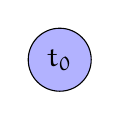
\begin{tikzpicture}[->,sibling distance=10em,
  every node/.style = {shape=circle, rounded corners,
    draw, align=center,minimum size=0.8cm, fill=black!20},
  cgreen/.style={fill=green!30},
  cblue/.style={fill=blue!30}]]
  \node[cblue] (1) at (0, 0) {$t_0$};
  \end{tikzpicture}
\end{center}

对于字符串 \(s=``a"\):
\begin{center}
  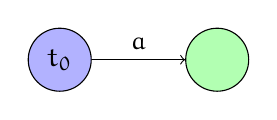
\begin{tikzpicture}[->,sibling distance=10em,
  every node/.style = {shape=circle, rounded corners,
    draw, align=center,minimum size=0.8cm, fill=black!20},
  cgreen/.style={fill=green!30},
  cblue/.style={fill=blue!30}]]
  \node[cblue] (1) at (0, 0) {$t_0$};
  \node[cgreen] (2) at (2, 0) {};
  \path[every node/.style={font=\sffamily\small}]
  (1) edge node[above] {$a$} (2);
  \end{tikzpicture}
\end{center}

对于字符串 \(s=``aa"\):
\begin{center}
  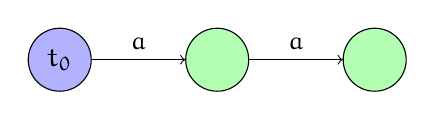
\begin{tikzpicture}[->,sibling distance=10em,
  every node/.style = {shape=circle, rounded corners,
    draw, align=center,minimum size=0.8cm, fill=black!20},
  cgreen/.style={fill=green!30},
  cblue/.style={fill=blue!30}]]
  \node[cblue] (1) at (0, 0) {$t_0$};
  \node[cgreen] (2) at (2, 0) {};
  \node[cgreen] (3) at (4, 0) {};
  \path[every node/.style={font=\sffamily\small}]
  (1) edge node[above] {$a$} (2)
  (2) edge node[above] {$a$} (3);
  \end{tikzpicture}
\end{center}

对于字符串 \(s=``ab"\):
\begin{center}
  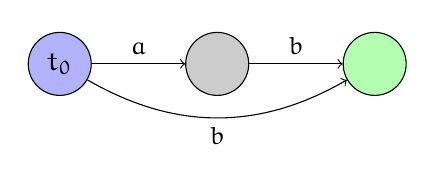
\begin{tikzpicture}[->,sibling distance=10em,
  every node/.style = {shape=circle, rounded corners,
    draw, align=center,minimum size=0.8cm, fill=black!20},
  cgreen/.style={fill=green!30},
  cblue/.style={fill=blue!30}]]
  \node[cblue] (1) at (0, 0) {$t_0$};
  \node (2) at (2, 0) {};
  \node[cgreen] (3) at (4, 0) {};
  \path[every node/.style={font=\sffamily\small}]
  (1) edge node[above] {$a$} (2)
  (2) edge node[above] {$b$} (3)
  (1) edge[bend right] node[below] {$b$} (3);
  \end{tikzpicture}
\end{center}

对于字符串 \(s=``abb"\):
\begin{center}
  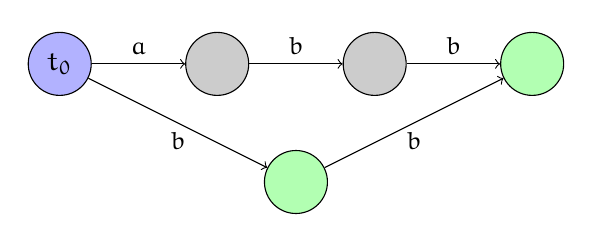
\begin{tikzpicture}[->,sibling distance=10em,
  every node/.style = {shape=circle, rounded corners,
    draw, align=center,minimum size=0.8cm, fill=black!20},
  cgreen/.style={fill=green!30},
  cblue/.style={fill=blue!30}]]
  \node[cblue] (1) at (0, 0) {$t_0$};
  \node (2) at (2, 0) {};
  \node (3) at (4, 0) {};
  \node[cgreen] (4) at (6, 0) {};
  \node[cgreen] (5) at (3, -1.5) {};
  \path[every node/.style={font=\sffamily\small}]
  (1) edge node[above] {$a$} (2)
  (2) edge node[above] {$b$} (3)
  (3) edge node[above] {$b$} (4)
  (1) edge node[below] {$b$} (5)
  (5) edge node[below] {$b$} (4);
  \end{tikzpicture}
\end{center}

对于字符串 \(s=``abbb"\):

\begin{center}
  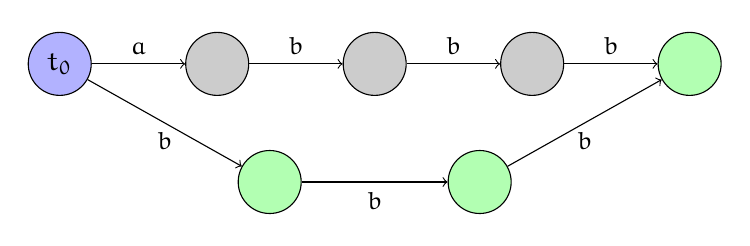
\begin{tikzpicture}[->,sibling distance=10em,
  every node/.style = {shape=circle, rounded corners,
    draw, align=center,minimum size=0.8cm, fill=black!20},
  cgreen/.style={fill=green!30},
  cblue/.style={fill=blue!30}]]
  \node[cblue] (1) at (0, 0) {$t_0$};
  \node (2) at (2, 0) {};
  \node (3) at (4, 0) {};
  \node (4) at (6, 0) {};
  \node[cgreen] (5) at (8, 0) {};
  \node[cgreen] (6) at (2.6666, -1.5) {};
  \node[cgreen] (7) at (5.3333, -1.5) {};
  \path[every node/.style={font=\sffamily\small}]
  (1) edge node[above] {$a$} (2)
  (2) edge node[above] {$b$} (3)
  (3) edge node[above] {$b$} (4)
  (4) edge node[above] {$b$} (5)
  (1) edge node[below] {$b$} (6)
  (6) edge node[below] {$b$} (7)
  (7) edge node[below] {$b$} (5);
  \end{tikzpicture}
\end{center}

\subsection{在线性时间内构造后缀自动机}

在我们描述线性时间内构造后缀自动机的算法之前,我们需要引入几个对理解构造过程非常重要的新概念并简单证明。

\subsubsection{结束位置 $endpos$}

考虑字符串  $s$ 的任意非空子串 $t$,我们记 $endpos(t)$ 为在字符串 $s$ 中 $t$ 的所有结束位置(假设对字符串中
字符的编号从零开始)。例如,对于字符串 ``abcbc",我们有 $endpos(``bc")=2,\,4$。

当两个子串 \(t_1\) 与 \(t_2\) 的末尾集合相等时我们称它们是 \(endpos\)
等价的:即 \(endpos(t_1)=endpos(t_2)\)。这样所有字符串 \(s\)
的非空子串都可以根据它们的 \textbf{\(endpos\)}
集合被分为几个\textbf{等价类}。

显然,在后缀自动机中的每个状态对应于一个或多个 \(endpos\)
相同的子串。换句话说,后缀自动机中的状态数等于所有子串的等价类的个数,加上初始状态。后缀自动机的状态个数等价于
\(endpos\) 相同的一个或多个子串。

我们稍后将会用这个假设介绍构造后缀自动机的算法。在那时我们将会发现,后缀自动机需要满足的所有性质,除了最小性以外都满足了。由 Nerode 定理我们可以得出最小性(这篇文章不会证明后缀自动机的最小性)。

由 \(endpos\) 的值我们可以得到一些重要结论:

\begin{quote}
\textbf{引理 1:}当且仅当字符串 \(u\) 以 \(w\)
的一个后缀的形式出现在字符串 \(s\) 中时,两个非空子串 \(u\) 和
\(w\)(假设 \(length(u)\le length(w)\))是 \(endpos\) 等价的。
\end{quote}

引理显然成立。如果 \(u\) 和 \(v\) 的 \(endpos\) 相同,则 \(u\) 是 \(w\)
的一个后缀,且只以 \(s\) 中的一个 \(w\)
的后缀的形式出现。且根据定义,如果 \(u\) 为 \(w\)
的一个后缀,且只以后缀的形式在 \(s\) 中出现时,两个子串的 \(endpos\)
值相等。

\begin{quote}
\textbf{引理 2:}考虑两个非空子串 \(u\) 和 \(w\)(假设
\(length(u)\le length(w)\))。则它们的 \(endpos\)
构成的集合要么完全没有交集,要么 \(endpos(w)\) 是 \(endpos(u)\)
的一个子集。并且这依赖于 \(u\) 是否为 \(w\) 的一个后缀。即:
\begin{equation*}
\begin{cases}
 endpos(w)\subseteq endpos(u)&\text{若 $u$ 为 $w$ 的一个后缀}\\
 endpos(w)\cap endpos(u)=\emptyset&\text{另一种情况}\\
\end{cases}
\end{equation*}
\end{quote}

证明:如果集合 \(endpos(u)\) 与 \(endpos(w)\)
有至少一个公共元素,那么由于字符串 \(u\) 与 \(w\) 都在一个位置结束,即
\(u\) 是 \(w\) 的一个后缀。但是如果如此在每次 \(w\) 出现的位置子串 \(u\)
也会出现,这意味着 \(endpos(w)\) 是 \(endpos(u)\) 的一个子集。

\begin{quote}
\textbf{引理 3:}考虑一个 \(endpos\)
等价类。将类中的所有子串按长度非递增的顺序排序。即每个子串都会比它前一个子串短,与此同时每个子串也是它前一个子串的一个后缀。换句话说,同一等价类中的所有子串均互为后缀,且子串的长度恰好覆盖整个区间
\([x,\,y]\)。
\end{quote}

证明:固定一些 \(endpos\)
等价类。如果等价类中只包含一个子串,引理显然成立。现在我们来讨论子串元素个数大于
\(1\) 的等价类。

由引理 1,两个不同的 \(endpos\)
等价字符串中较短的一个总是较长的一个的真后缀。因此,等价类中不可能有两个等长的字符串。

记 \(w\) 为等价类中最长的字符串,类似地,记 \(u\)
为等价类中最短的字符串。由引理 1,字符串 \(u\) 是字符串 \(w\)
的真后缀。现在考虑长度在区间 \([length(u),\,length(w)]\) 中的 \(w\)
的任意后缀。容易看出,这个后缀也在同一等价类中。因为这个后缀只能在字符串
\(s\) 中以 \(w\) 的一个后缀的形式存在(也因为较短的后缀 \(u\) 在 \(s\)
中只以 \(w\) 的后缀的形式存在)。因此,由引理 1,这个后缀与字符串 \(w\)
\(endpos\) 等价。

\subsubsection{后缀链接}

考虑后缀自动机中满足 \(v\ne t_0\) 的一些状态。我们已经知道,状态 \(v\)
对应于具有相同 \(endpos\) 的等价类。我们如果定义 \(w\)
为这些字符串中最长的一个,则所有其它的字符串都是 \(w\) 的后缀。

我们还知道字符串 \(w\)
的前几个后缀(如果我们用长度降序考虑这些后缀)在这个等价类中全部被包含,且所有其它后缀(至少一个---空后缀)在其它的等价类中。我们记
\(t\) 为最大的这样的后缀,然后用后缀链接连到 \(t\) 上。

换句话说,一个\textbf{后缀链接} \(link(v)\) 连接到对应于 \(w\)
的最长后缀的另一个 \(endpos\) 等价类的状态。

以下我们假设初始状态 \(t_0\)
对应于它自己这个等价类(只包含一个空字符串),为了方便我们规定
\(endpos(t)=\{-1,\,0,\,\ldots,\,length(s)-1\}\)。

\begin{quote}
\textbf{引理 4:}所有后缀链接构成一棵根节点为 \(t_0\) 的树。
\end{quote}

证明:考虑任意满足 \(v\ne t_0\) 的状态,一个后缀链接 \(link(v)\)
连接到的状态对应于严格更短的字符串(根据后缀链接的定义和引理
3)。因此,通过在后缀链接上移动,我们早晚会到达对应空串的初始状态
\(t_0\)。

\begin{quote}
\textbf{引理 5:}如果我们使用集合 \(endpos\)
构造一棵树(所有子节点的集合为父节点的子集),则这个结构由后缀链接连接起来。
\end{quote}

证明:由引理 2,我们可以用 \(endpos\)
集合构造一棵树(因为两个集合要么完全没有交集要么互为子集)。

我们现在考虑任意满足 \(v\ne t_0\) 的状态和它的后缀链接
\(link(v)\),由后缀链接和引理 2,我们可以得到
\[
endpos(v)\subseteq endpos(link(v))
\]
,这与前面的引理证明了以下断言成立:后缀链接构成的树本质上是 \(endpos\)
集合构成的一棵树。

以下是对于字符串 \(``abcbc"\)
构造后缀自动机时产生的后缀链接树的一个\textbf{例子},节点被标记为对应等价类中最长的子串。
\begin{center}
  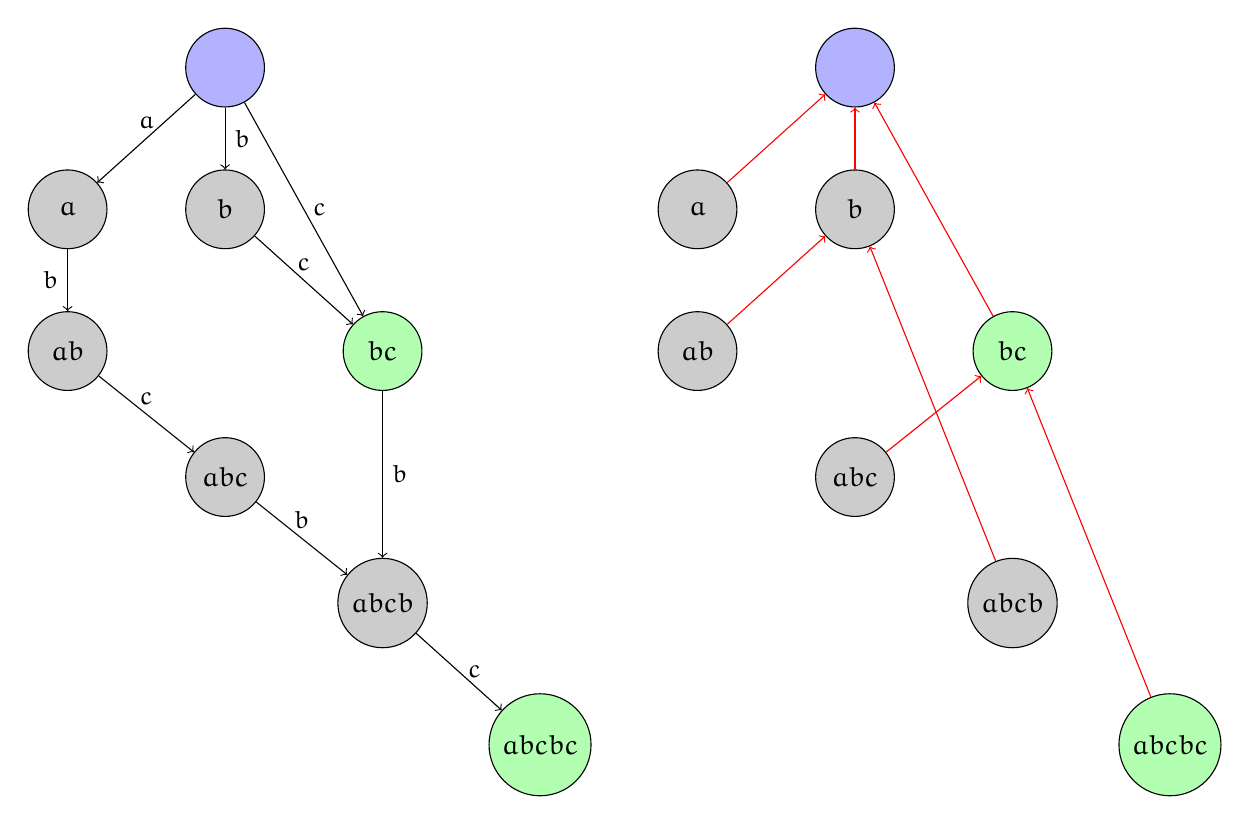
\begin{tikzpicture}[->,sibling distance=10em,
  every node/.style = {shape=circle, rounded corners,
    draw, align=center,minimum size=1.0cm, fill=black!20},
  cgreen/.style={fill=green!30},
  cblue/.style={fill=blue!30}]]
  \node[cblue] (1) at (0, 0) {$$};
  \node (2) at (-2, -1.8) {$a$};
  \node (3) at (0, -1.8) {$b$};
  \node[cgreen] (4) at (2, -3.6) {$bc$};
  \node (5) at (-2, -3.6) {$ab$};
  \node (6) at (0, -5.2) {$abc$};
  \node (7) at (2, -6.8) {$abcb$};
  \node[cgreen] (8) at (4, -8.6) {$abcbc$};
  \path[every node/.style={font=\sffamily\small}]
  (1) edge node[above] {$a$} (2)
  (1) edge node[right] {$b$} (3)
  (1) edge node[right] {$c$} (4)
  (2) edge node[left] {$b$} (5)
  (5) edge node[above] {$c$} (6)
  (6) edge node[above] {$b$} (7)
  (4) edge node[right] {$b$} (7)
  (7) edge node[right] {$c$} (8)
  (3) edge node[above] {$c$} (4);
  \node[cblue] (l1) at (8, 0) {$$};
  \node (l2) at (6, -1.8) {$a$};
  \node (l3) at (8, -1.8) {$b$};
  \node[cgreen] (l4) at (10, -3.6) {$bc$};
  \node (l5) at (6, -3.6) {$ab$};
  \node (l6) at (8, -5.2) {$abc$};
  \node (l7) at (10, -6.8) {$abcb$};
  \node[cgreen] (l8) at (12, -8.6) {$abcbc$};
  \path[every node/.style={font=\sffamily\small}]
  (l2) edge[red] node[above] {} (l1)
  (l3) edge[red] node[right] {} (l1)
  (l4) edge[red] node[right] {} (l1)
  (l5) edge[red] node[left] {} (l3)
  (l6) edge[red] node[above] {} (l4)
  (l7) edge[red] node[right] {} (l3)
  (l8) edge[red] node[above] {} (l4);
  \end{tikzpicture}
\end{center}

\subsubsection{小结}

在学习算法本身前,我们对之前学过的知识进行一下总结,并引入一些辅助记号。

\begin{itemize}
\item
  \(s\) 的子串可以根据它们结束的位置 \(endpos\) 被划分为多个等价类;
\item
  后缀自动机由初始状态 \(t_0\) 和与每一个 \(endpos\)
  等价类对应的每个状态组成;
\item
  对于每一个状态 \(v\),一个或多个子串与之匹配。我们记 \(longest(v)\)
  为其中最长的一个字符串,记 \(len(v)\) 为它的长度。类似地,记
  \(shortest(v)\) 为最短的子串,它的长度为
  \(minlen(v)\)。那么所有对应这个状态的所有字符串都是字符串
  \(longest(v)\) 的不同的后缀,且所有字符串的长度恰好覆盖区间
  \([minlength(v),\,len(v)]\) 中的每一个整数。
\item
  对于任意满足 \(v\ne t_0\) 的状态,定义后缀链接为连接到对应字符串
  \(longest(v)\) 的长度为 \(minlen(v)-1\) 的后缀的一条边。从根节点
  \(t_0\) 出发的后缀链接可以形成一棵树,与此同时,这棵树形成了
  \(endpos\) 集合间的包含关系。
\item
  我们可以对 \(v\ne t_0\) 的状态使用后缀链接 \(link(v)\) 解释
  \(minlen(v)\) 如下:
\[
minlen(v)=len(link(v))+1.
\]
\item
  如果我们从任意状态 \(v_0\) 开始顺着后缀链接遍历,早晚都会到达初始状态
  \(t_0\)。这种情况下我们可以得到一个互不相交的区间
  \([minlen(v_i),\,len(v_i)]\) 的序列,且它们的并集形成了连续的区间
  \([0,\,len(v_0)]\)。
\end{itemize}

\subsubsection{算法}

现在我们可以学习算法本身了。这个算法是\textbf{在线}算法,这意味着我们可以逐个加入字符串中的每个字符,并且在每一步中对应地维护后缀自动机。

为了保证线性的空间复杂度,我们将只保存 \(len\) 和 \(link\)
的值和每个状态的一个转移列表,我们不会标记终止状态(但是我们稍后会展示在构造后缀自动机后如何分配这些标记)。

一开始后缀自动机只包含一个状态 \(t_0\),编号为 \(0\)(其它状态的编号为
\(1,\,2,\,\ldots\))。为了方便,我们分配给它 \(len=0\) 和
\(link=-1\)(\(-1\) 表示一个虚拟的不存在的状态)。

现在整个任务转化为实现给当前字符串添加一个字符 \(c\)
的过程。算法流程如下:

\begin{itemize}
\item
  令 \(last\) 为对应添加字符 \(c\) 之前的整个字符串(一开始我们设置
  \(last=0\) 且我们会在算法的最后一步对应地更新 \(last\))。
\item
  创建一个新的状态 \(cur\),并将 \(len(cur)\) 赋值为
  \(len(last)+1\),在这时 \(link(cur)\) 的值还未知。
\item
  现在我们按以下流程进行:我们从状态 \(last\) 开始。如果还没有到字符
  \(c\) 的转移,我们就添加一个到状态 \(cur\)
  的转移,遍历后缀链接。如果在某个点已经存在到字符 \(c\)
  的后缀链接,我们就停下来,并将这个状态标记为 \(p\)。
\item
  如果没有找到这样的状态 \(p\),我们就到达了虚拟状态 \(-1\),我们将
  \(link(cur)\) 赋值为 \(0\) 并退出。
\item
  假设现在我们找到了一个状态 \(p\),其可以转移到字符
  \(c\),我们将这个状态转移到的状态标记为 \(q\)。
\item
  现在我们分类讨论两种状态,要么 \(len(p) + 1 = len(q)\),要么不是。
\item
  如果 \(len(p)+1=len(q)\),我们只要将 \(link(cur)\) 赋值为 \(q\)
  并退出。
\item
  否则就会有些复杂。需要\textbf{复制}状态 \(q\):我们创建一个新的状态
  \(clone\),复制 \(q\) 的除了 \(len\)
  的值以外的所有信息(后缀链接和转移)。我们将 \(len(clone)\) 赋值为
  \(len(p)+1\)。\\
  复制之后,我们将后缀链接从 \(cur\) 指向 \(clone\),也从 \(q\) 指向
  \(clone\)。\\
  最终我们需要使用后缀链接从状态 \(p\) 返回,因为存在一条通过 \(c\)
  到状态 \(q\) 的转移,并在此过程中重定向所有状态到状态 \(clone\)。
\item
  以上三种情况,在完成这个过程之后,我们将 \(last\) 的值更新为状态
  \(cur\)。
\end{itemize}

如果我们还想知道哪些状态是\textbf{终止状态}而哪些不是,我们可以在为字符串
\(s\)
构造完完整的后缀自动机后找到所有的终止状态。为此,我们从对应整个字符串的状态(存储在变量
\(last\)
中),遍历它的后缀链接,直到到达初始状态。我们将所有遍历到的节点都标记为终止节点。容易理解这样做我们会精确地标记字符串
\(s\) 的所有后缀,这些状态恰好是终止状态。

在下一部分,我们将观察算法每一步的细节,并证明它的\textbf{正确性}。

现在,我们只注意到,因为我们只为 \(s\)
的每个字符创建一个或两个新状态所以后缀自动机只包含\textbf{线性个}状态。

转移个数是线性规模的,以及总体上算法的运行时间是线性规模的,这两点还不那么清
楚。

\subsubsection{正确性证明}

\begin{itemize}
\item
  若一个转移 \((p,\,q)\) 满足 \(len(p)+1=len(q)\)
  则我们称这个转移是\textbf{连续的}。否则,即当 \(len(p)+1<len(q)\)
  时,这个转移被称为\textbf{不连续的}。
  从算法描述中可以看出,连续的和非连续的转移是算法的不同情况。连续的转移是固定的,我们不会再改变了。与此相反,当向字符串中插入一个新的字符时,非连续的转移可能会改变(转移边的端点可能会改变)。
\item
  为了避免引起歧义,我们记向后缀自动机中插入当前字符 \(c\)
  之前的字符串为 \(s\)。
\item
  算法从创建一个新状态 \(cur\) 开始,对应于整个字符串
  \(s+c\)。我们创建一个新的节点的原因很清楚。与此同时我们也创建了一个新的字符和一个新的等价类。
\item
  在创建一个新的状态之后,我们会从对应于整个字符串 \(s\)
  的状态通过后缀链接进行遍历。对于每一个状态,我们尝试添加一个从字符
  \(c\) 到新状态 \(cur\)
  的转移。然而我我们只能添加与原来已存在的转移不冲突的转移。因此我们只要找到已存在的
  \(c\) 的转移,我们就必须停止。
\item
  最简单的情况是我们到达了虚拟状态 \(-1\),这意味着我们为所有 \(s\)
  的后缀添加了 \(c\) 的转移。这也意味着,字符 \(c\) 从未在字符串 \(s\)
  中出现过。因此 \(cur\) 的后缀链接为状态 \(0\)。
\item
  第二种情况下,我们找到了现有的转移
  \((p,\,q)\)。这意味着我们尝试向自动机内添加一个\textbf{已经存在的}字符串
  \(x+c\)(其中 \(x\) 为 \(s\) 的一个后缀,且字符串 \(x+c\) 已经作为
  \(s\) 的一个子串出现过了)。因为我们假设字符串 \(s\)
  的自动机的构造是正确的,我们不应该在这里添加一个新的转移。
  然而,有一个难点。从状态 \(cur\)
  出发的后缀链接应该连接到哪个状态呢?我们要把后缀链接连到一个状态上,且其中最长的一个字符串恰好是
  \(x+c\),即这个状态的 \(len\) 应该是
  \(len(p)+1\)。然而还不存在这样的状态,即
  \(len(q)>len(p)+1\)。这种情况下,我们必须要通过拆开状态 \(q\)
  来创建一个这样的状态。
\item
  如果转移 \((p,\,q)\) 是连续的,那么
  \(len(q)=len(p)+1\)。在这种情况下一切都很简单。我们只需要将 \(cur\)
  的后缀链接指向状态 \(q\)。
\item
  否则转移是不连续的,即 \(len(q)>len(p)+1\),这意味着状态 \(q\)
  不只对应于长度为\(len(p)+1\) 的后缀 \(s+c\),还对应于 \(s\)
  的更长的子串。除了将状态 \(q\)
  拆成两个子状态以外我们别无他法,所以第一个子状态的长度就是
  \(len(p)+1\) 了。\\
  我们如何拆开一个状态呢?我们\textbf{复制}状态 \(q\),产生一个状态
  \(clone\),我们将 \(len(clone)\) 赋值为
  \(len(p)+1\)。由于我们不想改变遍历到 \(q\) 的路径,我们将 \(q\)
  的所有转移复制到 \(clone\)。我们也将从 \(clone\) 出发的后缀链接设置为
  \(q\) 的后缀链接的目标,并设置 \(q\) 的后缀链接为 \(clone\)。\\
  在拆开状态后,我们将从 \(cur\) 出发的后缀链接设置为 \(clone\)。\\
  最后一步我们将一些到 \(q\) 转移重定向到
  \(clone\)。我们需要修改哪些转移呢?只重定向相当于所有字符串
  \(w+c\)(其中 \(w\) 是 \(p\)
  的最长字符串)的后缀就够了。即,我们需要继续沿着后缀链接遍历,从顶点
  \(p\) 直到虚拟状态 \(-1\) 或者是转移到不是状态 \(q\) 的一个转移。
\end{itemize}

\subsubsection{对操作次数为线性的证明}

首先我们假设字符集大小为\textbf{常数}。如果字符集大小不是常数,后缀自动机的时间复杂度就不是线性的。从一个顶点出发的转移存储在支持快速查询和插入的平衡树中。因此如果我们记
\(k\) 为字符集的大小,则算法的渐进时间复杂度为
\(O(n\log k)\),空间复杂度为
\(O(n)\)。然而如果字符集足够小,可以不写平衡树,以空间换时间将每个顶点的转移存储为长度为
\(k\)
的数组(用于快速查询)和链表(用于快速遍历所有可用关键字)。这样算法的时间复杂度为
\(O(n)\),空间复杂度为 \(O(nk)\)。

所以我们将认为字符集的大小为常数,即每次对一个字符搜索转移、添加转移、查找下一个转移---这些操作的时间复杂度都为
\(O(1)\)。

如果我们考虑算法的各个部分,算法中有三处时间复杂度不明显是线性的:
\begin{itemize}
\item
  第一处是遍历所有状态 \(last\) 的后缀链接,添加字符 \(c\) 的转移。
\item
  第二处是当状态 \(q\) 被复制到一个新的状态 \(clone\) 时复制转移的过程。
\item
  第三处是修改指向 \(q\) 的转移,将它们重定向到 \(clone\) 的过程。
\end{itemize}

我们使用后缀自动机的大小(状态数和转移数)为\textbf{线性的}的事实(对状态数是线性的的证明就是算法本身,对状态数为线性的的证明将在稍后实现算法后给出)。

因此上述\textbf{第一处和第二处}的总复杂度显然为线性的,因为单次操作均摊只为自动机添加了一个新转移。

还需为\textbf{第三处}估计总复杂度,我们将最初指向 \(q\) 的转移重定向到
\(clone\)。我们记 \(v=longest(p)\),这是一个字符串 \(s\)
的后缀,每次迭代长度都递减---因为作为字符串 \(s\)
的位置随着每次迭代都单调上升。这种情况下,如果在循环的第一次迭代之前,相对应的字符串
\(v\) 在距离 \(last\) 的深度为 \(k\) \((k\ge2)\)
的位置上(深度记为后缀链接的数量),那么在最后一次迭代后,字符串 \(v+c\)
将会成为路径上第二个从 \(cur\) 出发的后缀链接(它将会成为新的 \(last\)
的值)。

因此,循环中的每次迭代都会使作为当前字符串的后缀的字符串
\(longest(link(link(last))\)
的位置单调递增。因此这个循环最多不会执行超过 \(n\)
次迭代,这正是我们需要证明的。

\subsubsection{实现}

首先,我们描述一种存储一个转移的全部信息的数据结构。如果需要的话,你可以在这里加入一个终止标记,也可以是一些其它信息。我们将会用一个
\texttt{map} 存储转移的列表,允许我们在总计 \(O(n)\) 的空间复杂度和
\(O(n\log k)\) 的时间复杂度内处理整个字符串。
\begin{minted}{C++}
struct state {
  int len, link;
  map<char, int> next;
};
\end{minted}

后缀自动机本身将会存储在一个 \texttt{state}
结构体数组中。我们记录当前自动机的大小 \texttt{sz} 和变量
\texttt{last},当前整个字符串对应的状态。
\begin{minted}{C++}
const int MAXLEN = 100000;
state st[MAXLEN * 2];
int sz, last;
\end{minted}

我们定义一个函数来初始化后缀自动机(创建一个只有一个状态的后缀自动机)。
\begin{minted}{C++}
void sa_init() {
  st[0].len = 0;
  st[0].link = -1;
  sz++;
  last = 0;
}
\end{minted}

最终我们给出主函数的实现---给当前行末增加一个字符,对应地重建自动机。

\begin{minted}{C++}
void sa_extend(char c) {
  int cur = sz++;
  st[cur].len = st[last].len + 1;
  int p = last;
  while (p != -1 && !st[p].next.count(c)) {
    st[p].next[c] = cur;
    p = st[p].link;
  }
  if (p == -1) {
    st[cur].link = 0;
  } else {
    int q = st[p].next[c];
    if (st[p].len + 1 == st[q].len) {
      st[cur].link = q;
    } else {
      int clone = sz++;
      st[clone].len = st[p].len + 1;
      st[clone].next = st[q].next;
      st[clone].link = st[q].link;
      while (p != -1 && st[p].next[c] == q) {
        st[p].next[c] = clone;
        p = st[p].link;
      }
      st[q].link = st[cur].link = clone;
    }
  }
  last = cur;
}
\end{minted}

正如之前提到的一样,如果你用内存换时间(空间复杂度为 \(O(nk)\),其中
\(k\) 为字符集大小),你可以在 \(O(n)\) 的时间内构造字符集大小 \(k\)
任意的后缀自动机。但是这样你需要为每一个状态储存一个大小为 \(k\)
的数组(用于快速跳转到转移的字符),和另外一个所有转移的链表(用于快速在转移中迭代)。

\subsection{更多的性质}

\subsubsection{状态数}

对于一个长度为 \(n\) 的字符串
\(s\),它的后缀自动机中的状态数\textbf{不会超过 \(2n-1\)} (假设
\(n\ge2\))。

对上述结论的证明就是算法本身,因为一开始自动机含有一个状态,第一次和第二次迭代中只会创建一个节点,剩余的
\(n-2\) 步中每步会创建至多 \(2\) 个状态。

然而我们也能在\textbf{不知道这个算法}的情况下\textbf{展示}这个估计值。我们回忆一下状态数等于不同的
\(endpos\) 集合个数。另外这些 \(endpos\)
集合形成了一棵树(祖先节点的集合包含了它所有孩子节点的集合)。考虑将这棵树稍微变形一下:只要它有一个只有一个孩子的内部顶点(这意味着该子节点的集合至少遗漏了它的父集合中的一个位置),我们创建一个含有这个遗漏位置的集合。最后我们可以获得一棵每一个内部顶点的度数大于一的树,并且叶子节点的个数不超过
\(n\)。因此这样的树里有不超过 \(2n-1\) 个节点。

对于每个确定的 \(n\),状态数的上界是确定的。一个可能的字符串是:
\[
``abbb\ldots bbb"
\]
从第三次迭代后的每次迭代,算法都会拆开一个状态,最终产生恰好 \(2n-1\)
个状态。

\subsubsection{转移数}

对于一个长度为 \(n\) 的字符串
\(s\),它的后缀自动机中的转移数\textbf{不会超过 \(3n-4\)}(假设
\(n\ge 3\))。

证明如下:

我们首先估计连续的转移的数量。考虑自动机中从状态 \(t_0\)
开始的最长路径的生成树。生成树的骨架只包含连续的边,因此数量少于状态数,即,边数不会超过
\(2n-2\)。

现在我们来估计非连续的转移的数量。令当前非连续转移为
\((p,\,q)\),其字符为 \(c\)。我们取它的对应字符串 \(u+c+w\),其中字符串
\(u\) 对应于初始状态到 \(p\) 的最长路径,\(w\) 对应于从 \(p\)
到任意终止状态的最长路径。一方面,对于每个不完整的字符串所对应的形如
\(u+c+w\) 的字符串是不同的(因为字符串 \(u\) 和 \(w\)
仅由完整的转移组成)。另一方面,由终止状态的定义,每个形如 \(u+c+w\)
的字符串都是整个字符串 \(s\) 的后缀。因为 \(s\) 只有 \(n\)
个非空后缀,且形如 \(u+c+w\) 的字符串都不包含
\(s\)(因为整个字符串只包含完整的转移),所以非完整的转移的总数不会超过
\(n-1\)。

将以上两个估计值结合起来,我们可以得到上界
\(3n-3\)。然而,最大的状态数只能在测试数据 ``abbb\ldots bbb"
中产生,这个测试数据的转移数量显然少于
\(3n-3\),我们可以获得更为紧确的后缀自动机的转移数的上界:\(3n-4\)。

上界可以通过字符串
\[
``abbb\ldots bbbc"
\]
达到。

\subsection{应用}

下面我们来看一下一些可以用后缀自动机解决的问题。为了简单,我们假设字符集的大小
\(k\) 为常数,允许我们认为增加一个字符和遍历的复杂度为常数。

\subsubsection{检查字符串是否出现}

\begin{quote}
给一个文本串 \(T\) 和多个模式串 \(P\),我们要检查字符串 \(P\) 是否作为
\(T\) 的一个子串出现。
\end{quote}

我们在 \(O(length(T))\) 的时间内为文本串 \(T\)
构造后缀自动机。为了检查模式串 \(T\) 是否在 \(T\)
中出现,我们沿转移(边)从 \(t_0\) 开始根据 \(P\)
的字符进行转移。如果在某个点无法转移下去,则模式串 \(P\) 不是 \(T\)
的一个子串。如果我们能够这样处理完整个字符串 \(P\),那么模式串在 \(T\)
中出现过。因此

对于每个字符串 \(P\) 算法的时间复杂度为
\(O(length(P))\)。此外,这个算法还找到了模式串 \(P\)
在文本串中出现的最大前缀长度。

\subsubsection{不同子串个数}

\begin{quote}
给一个字符串 \(S\),计算不同子串的个数。
\end{quote}

为字符串 \(S\) 构造后缀自动机。

每个 \(S\)
的子串都相当于自动机中的一些路径。因此不同子串的个数等于自动机中以
\(t_0\) 为起点的不同路径的条数。

考虑到后缀自动机为有向无环图,不同路径的条数可以使用动态规划计算。

即,令 \(d[v]\) 为从状态 \(v\)
开始的路径数量(包括长度为零的路径),则我们有如下递推方程式:
\[
d[v]=1+\sum_{w:(v,\,w,\,c)\in SA}d[w]
\]
即,\(d[v]\) 可以表示为所有 \(v\) 的转移的末端的和。

所以不同子串的个数为 \(d[t_0]-1\)(因为要去掉空子串)。

总时间复杂度为:\(O(length(S))\)。

\subsubsection{所有不同子串的总长度}

\begin{quote}
给定一个字符串 \(S\),计算所有不同子串的总长度。
\end{quote}

本题做法与上一题类似,只是现在我们需要考虑分两部分进行动态规划:不同子串的数量
\(d[v]\) 和它们的总长度 \(ans[v]\)。

我们已经在上一题中介绍了如何计算 \(d[v]\)。\(ans[v]\)
的值可以使用通过以下递推式计算:
\[
ans[v]=\sum_{w:(v,\,w,\,c)\in DAWG}d[w]+ans[w]
\]
我们取每个邻接顶点 \(w\) 的答案,并加上 \(d[w]\)(因为从状态 \(v\)
出发的子串都增加了一个字符)。

算法的时间复杂度仍然是 \(O(length(S))\)。

\subsubsection{字典序第$k$大子串}

\begin{quote}
给定一个字符串 \(S\)。多组询问,每组询问给定一个数
\(K_i\),查询所有子串中词典序第 \(k\) 大的子串。
\end{quote}

解决这个问题的思路基于前两个问题的思路。字典序第 \(k\)
大的子串对应于后缀自动机中字典序第 \(k\)
大的路径。因此在计算每个状态的路径数后,我们可以很容易地从后缀自动机的根开始找到第
\(k\) 大的路径。

预处理的时间复杂度为 \(O(length(S))\),单次查询的复杂度为
\(O(length(ans)\cdot k)\)(其中 \(ans\) 是查询的答案,\(k\)
为字符集的大小)。

\subsubsection{最小循环移位}

\begin{quote}
给定一个字符串 \(S\)。找出字典序最小的循环移位。
\end{quote}

我们为字符串 \(S+S\) 构造后缀自动机。则后缀自动机本身将包含字符串 \(S\)
的所有循环移位作为路径。

所以问题简化为寻找最小的长度为 \(length(S)\)
的路径,这可以通过平凡的方法做到:我们从初始状态开始,贪心地访问最小的字符即可。

总的时间复杂度为 \(O(length(S))\)。

\subsubsection{出现次数}

\begin{quote}
对于一个给定的文本串 \(T\),有多组询问,每组询问给一个模式串
\(P\),回答模式串 \(P\) 在字符串 \(T\) 中作为子串出现了多少次。
\end{quote}

我们为文本串 \(T\) 构造后缀自动机。

接下来我们做以下的预处理:对于自动机中的每个状态 \(v\),预处理值等于
\(endpos(v)\) 这个集合大小的 \(cnt[v]\)。事实上对应于同一状态 \(v\)
的所有子串在文本串 \(T\) 中的出现次数相同,这相当于集合 \(endpos\)
中的位置数。

然而我们不能明确的构造集合 \(endpos\),因此我们只考虑它们的大小
\(cnt\)。

为了计算这些值,我们进行以下操作。对于每个状态,如果它不是通过复制创建的(且它不是初始状态
\(t_0\)),我们用 \(cnt=1\) 初始化它。然后我们按它们的长度 \(len\)
降序遍历所有状态,并将当前的 \(cnt[v]\) 的值加到后缀链接上,即:
\[
cnt[link(v)]+=cnt[v]
\]
这样做每个状态的答案都是正确的。

为什么这是正确的?通过复制获得的状态,恰好是
\(length(T)\),并且它们中的前 \(i\) 个在我们插入前 \(i\)
个字符时产生。因此对于每个这样的状态,我们在它被处理时计算它们所对应的位置的数量。因此我们初始将这些状态的
\(cnt\) 的值赋为 \(1\),其它状态的 \(cnt\) 值赋为 \(0\)。

接下来我们对每一个 \(v\)
执行以下操作:\(cnt[link(v)]+=cnt[v]\)。其背后的含义是,如果有一个字符串
\(v\) 出现了 \(cnt[v]\)
次,那么它的所有后缀也在完全相同的地方结束,即也出现了 \(cnt[v]\) 次。

为什么我们在这个过程中不会重复计数(即把某些位置数了两次)呢?因为我们只将一个状态的位置添加到\textbf{一个}其它的状态上,所以一个状态不可能以两种不同的方式将其位置重复地指向另一个状态。

因此,我们可以在 \(O(length(T))\) 的时间内计算出所有状态的 \(cnt\)
的值。

最后回答询问只需要查找查找值 \(cnt[t]\),其中 \(t\)
为如果存在这样的状态就是状态对应的模式串,如果不存在答案就为
\(0\)。单次查询的时间复杂度为 \(O(length(P))\)。

\subsubsection{第一次出现的位置}

\begin{quote}
给定一个文本串 \(T\),多组查询。每次查询字符串 \(P\) 在字符串 \(T\)
中第一次出现的位置(\(P\) 的开头位置)。
\end{quote}

我们再构造一个后缀自动机。我们对自动机中的所有状态预处理位置
\(firstpos\)。即,对每个状态 \(v\)
我们想要找到第一次出现这个状态的末端的位置
\(firstpos[v]\)。换句话说,我们希望先找到每个集合 \(endpos\)
中的最小的元素(显然我们不能显式地维护所有 \(endpos\) 集合)。

为了维护 \(firstpos\) 这些位置,我们将原函数扩展为
\texttt{sa\_extend()}。当我们创建新状态 \(cur\) 时,我们令:
\[
firstpos(cur)=len(cur)-1
\]
;当我们将顶点 \(q\) 复制到 \(clone\) 时,我们令:
\[
firstpos(clone)=firstpos(q)
\]
(因为值的唯一其它选项 \(firstpos(cur)\) 肯定太大了)。

那么查询的答案就是 \(firstpos(t)-length(P)+1\),其中 \(t\) 为对应字符串
\(P\) 的状态。单次查询只需要 \(O(length(P))\) 的时间。

\subsubsection{所有出现的位置}

\begin{quote}
问题同上,这一次需要查询文本串 \(T\) 中模式串出现的所有位置。
\end{quote}

我们还是为文本串 \(T\)
构造后缀自动机。与上一个问题相似地,我们为所有状态计算位置
\(firstpos\)。

如果 \(t\) 为对应于模式串 \(T\) 的状态,显然 \(firstpos(t)\)
为答案的一部分。需要查找的其它位置怎么办?我们使用了含有字符串 \(P\)
的自动机,我们还需要将哪些状态纳入自动机呢?所有对应于以 \(P\)
为后缀的字符串的状态。换句话说我们要找到所有可以通过后缀链接到达状态
\(t\) 的状态。

因此为了解决这个问题,我们需要为每一个状态保存一个指向它的后缀引用列表。查询的答案就包含了对于每个我们能从状态
\(t\) 只使用后缀引用进行 DFS 或 BFS 的所有状态的 \(firstpos\) 值。

这种变通方案的时间复杂度为
\(O(answer(P))\),因为我们不会重复访问一个状态(因为对于仅有一个后缀链接指向一个状态,所以不存在两条不同的路径指向同一状态)。

我们只需要考虑两个可能有相同 \(endpos\)
值的不同状态。如果一个状态是由另一个复制而来的,则这种情况会发生。然而,这并不会对复杂度分析造成影响,因为每个状态至多被复制一次。

此外,如果我们不从被复制的节点输出位置,我们也可以去除重复的位置。事实上对于一个状态,如果经过被复制状态可以到达,则经过原状态也可以到达。因此,如果我们给每个状态记录标记
\texttt{is\_clone},我们就可以简单地忽略掉被复制的状态,只输出其它所有状态的
\(firstpos\) 的值。

以下是实现的框架:

\begin{minted}{C++}
struct state {
  ... bool is_clone;
  int first_pos;
  vector<int> inv_link;
};

// 在构造后缀自动机后
for (int v = 1; v < sz; v++) {
  st[st[v].link].inv_link.push_back(v);
}

// 输出所有出现位置
void output_all_occurrences(int v, int P_length) {
  if (!st[v].is_clone) cout << st[v].first_pos - P_length + 1 << endl;
  for (int u : st[v].inv_link) output_all_occurrences(u, P_length);
}
\end{minted}

\subsubsection{最短的没有出现的字符串}

\begin{quote}
给定一个字符串 \(S\) 和一个特定的字符集,我们要找一个长度最短的没有在
\(S\) 中出现过的字符串。
\end{quote}

我们在字符串 \(S\) 的后缀自动机上做动态规划。

令 \(d[v]\) 为节点 \(v\)
的答案,即,我们已经处理完了子串的一部分,当前在状态
\(v\),想找到不连续的转移需要添加的最小字符数量。计算 \(d[v]\)
非常简单。如果不存在使用字符集中至少一个字符的转移,则
\(d[v]=1\)。否则添加一个字符是不够的,我们需要求出所有转移中的最小值:
\[
d[v]=1+\min_{w(v,\,w,\,c)\in SA}d[w]
\]
问题的答案就是 \(d[t_0]\),字符串可以通过计算过的数组 \(d[]\) 逆推回去。

\subsubsection{两个字符串的最长公共子串}

\begin{quote}
给定两个字符串 \(S\) 和 \(T\),求出最长公共子串,公共子串定义为在 \(S\)
和 \(T\) 中都作为子串出现过的字符串 \(X\)。
\end{quote}

我们为字符串 \(S\) 构造后缀自动机。

我们现在处理字符串 \(T\),对于每一个前缀都在 \(S\)
中寻找这个前缀的最长后缀。换句话说,对于每个字符串 \(T\)
中的位置,我们想要找到这个位置结束的 \(S\) 和 \(T\)
的最长公共子串的长度。

为了达到这一目的,我们使用两个变量,\textbf{当前状态} \(v\) 和
\textbf{当前长度}
\(l\)。这两个变量描述当前匹配的部分:它的长度和它们对应的状态。

一开始 \(v=t_0\) 且 \(l=0\),即,匹配为空串。

现在我们来描述如何添加一个字符 \(T[i]\) 并为其重新计算答案:

\begin{itemize}
\item
  如果存在一个从 \(v\) 到字符 \(T[i]\) 的转移,我们只需要转移并让 \(l\)
  自增一。
\item
  如果不存在这样的转移,我们需要缩短当前匹配的部分,这意味着我们需要按照以下后缀链接进行转移:
\[
v=link(v)
\]
与此同时,需要缩短当前长度。显然我们需要将 \(l\) 赋值为
\(len(v)\),因为经过这个后缀链接后我们到达的状态所对应的最长字符串是一个子串。
\item
  如果仍然没有使用这一字符的转移,我们继续重复经过后缀链接并减小
  \(l\),直到我们找到一个转移或到达虚拟状态 \(-1\)(这意味着字符
  \(T[i]\) 根本没有在 \(S\) 中出现过,所以我们设置 \(v=l=0\))。
\end{itemize}

问题的答案就是所有 \(l\) 的最大值。

这一部分的时间复杂度为 \(O(length(T))\),因为每次移动我们要么可以使
\(l\) 增加一,要么可以在后缀链接间移动几次,每次都减小 \(l\) 的值。

代码实现:

\begin{minted}{C++}
string lcs(string S, string T) {
  sa_init();
  for (int i = 0; i < S.size(); i++) sa_extend(S[i]);

  int v = 0, l = 0, best = 0, bestpos = 0;
  for (int i = 0; i < T.size(); i++) {
    while (v && !st[v].next.count(T[i])) {
      v = st[v].link;
      l = st[v].length;
    }
    if (st[v].next.count(T[i])) {
      v = st[v].next[T[i]];
      l++;
    }
    if (l > best) {
      best = l;
      bestpos = i;
    }
  }
  return t.substr(bestpos - best + 1, best);
}
\end{minted}

\subsubsection{多个字符串间的最长公共子串}

\begin{quote}
给定 \(k\) 个字符串
\(S_i\)。我们需要找到它们的最长公共子串,即作为子串出现在每个字符串中的字符串
\(X\)。
\end{quote}

我们将所有的子串连接成一个较长的字符串 \(T\),以特殊字符 \(D_i\)
分开每个字符串(一个字符对应一个字符串):
\[
T=S_1+D_1+S_2+D_2+\cdots+S_k+D_k.
\]
然后为字符串 \(T\) 构造后缀自动机。

现在我们需要在自动机中找到存在于所有字符串 \(S_i\)
中的一个字符串,这可以通过使用添加的特殊字符完成。注意如果 \(S_j\)
包含了一个子串,则后缀自动机中存在一条从包含字符 \(D_j\)
的子串而不包含以其它字符
\(D_1,\,\ldots,\,D_{j-1},\,D_{j+1},\,\ldots,\,D_k\) 开始的路径。

因此我们需要计算可达性,它告诉我们对于自动机中的每个状态和每个字符
\(D_i\) 是否存在这样的一条路径。这可以容易地通过 DFS 或 BFS
与动态规划计算。在此之后,问题的答案就是状态 \(v\) 的字符串
\(longest(v)\) 中存在所有特殊字符的路径。

\subsection{例题}

\begin{itemize}
\item
  SPOJ \#7258 SUBLEX
\item
  \href{http://hihocoder.com/problemset/problem/1441}{HihoCoder \#1441 :
  后缀自动机一 · 基本概念}
\end{itemize}

\subsection{相关资料}

我们先给出与后缀自动机有关的最初的一些文献:

\begin{itemize}
\item
  A. Blumer, J. Blumer, A. Ehrenfeucht, D. Haussler, R. McConnell.
  \textbf{Linear Size Finite Automata for the Set of All Subwords of a
  Word. An Outline of Results} {[}1983{]}
\item
  A. Blumer, J. Blumer, A. Ehrenfeucht, D. Haussler. \textbf{The
  Smallest Automaton Recognizing the Subwords of a Text} {[}1984{]}
\item
  Maxime Crochemore. \textbf{Optimal Factor Transducers} {[}1985{]}
\item
  Maxime Crochemore. \textbf{Transducers and Repetitions} {[}1986{]}
\item
  A. Nerode. \textbf{Linear automaton transformations} {[}1958{]}
\end{itemize}

另外,在更新的一些资源里,在很多关于字符串算法的书中,都能找到这个主题:

\begin{itemize}
\item
  Maxime Crochemore, Rytter Wowjcieh. \textbf{Jewels of Stringology}
  {[}2002{]}
\item
  Bill Smyth. \textbf{Computing Patterns in Strings} {[}2003{]}
\item
  Bill Smith. \textbf{Methods and algorithms of calculations on lines}
  {[}2006{]}
\end{itemize}

另外,还有一些资料:

\begin{itemize}
\item
  《后缀自动机》,陈立杰。
\item
  《后缀自动机在字典树上的拓展》,刘研绎。
\item
  《后缀自动机及其应用》,张天扬。
\item
  \url{https://www.cnblogs.com/zinthos/p/3899679.html}
\item
  \url{https://codeforces.com/blog/entry/20861}
\item
  \url{https://zhuanlan.zhihu.com/p/25948077}
\end{itemize}

\begin{center}\rule{0.5\linewidth}{\linethickness}\end{center}

\textbf{本页面主要译自博文
\href{http://e-maxx.ru/algo/suffix_automata}{Суффиксный автомат}
与其英文翻译版
\href{https://cp-algorithms.com/string/suffix-automaton.html}{Suffix
Automaton} 。其中俄文版版权协议为 Public Domain + Leave a
Link;英文版版权协议为 CC-BY-SA 4.0。}

\section{后缀树}



\section{Manacher}

\subsection{描述}

给定一个长度为 $n$ 的字符串 $s$,请找到所有对 $(i, j)$ 使得子串 $s[i \dots j]$ 为一个回文串。当 $t = t_{\text{rev}}$ 时,字符串 $t$ 是一个回文串($t_{\text{rev}}$ 是 $t$ 的反转字符串)。

\subsection{更进一步的描述}

显然在最坏情况下可能有 $O(n^2)$ 个回文串,因此似乎一眼看过去该问题并没有线性算法。

但是关于回文串的信息可用\textbf{一种更紧凑的方式}表达:对于每个位置 $i = 0 \dots n - 1$,我们找出值 $d_1[i]$ 和 $d_2[i]$。二者分别表示以位置 $i$ 为中心的长度为奇数和长度为偶数的回文串个数。

举例来说,字符串 $s = \mathtt{abababc}$ 以 $s[3] = b$ 为中心有三个奇数长度的回文串,也即 $d_1[3] = 3$:

$$
a\ \overbrace{b\ a\ \underset{s_3}{b}\ a\ b}^{d_1[3]=3}\ c
$$

字符串 $s = \mathtt{cbaabd}$ 以 $s[3] = a$ 为中心有两个偶数长度的回文串,也即 $d_2[3] = 2$:

$$
c\ \overbrace{b\ a\ \underset{s_3}{a}\ b}^{d_2[3]=2}\ d
$$

因此关键思路是,如果以某个位置 $i$ 为中心,我们有一个长度为 $l$ 的回文串,那么我们有以 $i$ 为中心的长度为 $l - 2$,$l - 4$,等等的回文串。所以 $d_1[i]$ 和 $d_2[i]$ 两个数组已经足够表示字符串中所有子回文串的信息。

一个令人惊讶的事实是,存在一个复杂度为线性并且足够简单的算法计算上述两个 “回文性质数组” $d_1[]$ 和 $d_2[]$。在这篇文章中我们将详细的描述该算法。

\subsection{解法}

总的来说,该问题具有多种解法:应用字符串哈希,该问题可在 $O(n \log n)$ 时间内解决,而使用后缀数组和快速 LCA 该问题可在 $O(n)$ 时间内解决。

但是这里描述的算法\textbf{压倒性}的简单,并且在时间和空间复杂度上具有更小的常数。该算法由\textbf{Glenn K. Manacher}在 1975 年提出。

\subsection{朴素算法}

为了避免在之后的叙述中出现歧义,这里我们指出什么是 “朴素算法”。

该算法通过下述方式工作:对每个中心位置 $i$,在比较一对对应字符后,只要可能,该算法便尝试将答案加 $1$。

该算法是比较慢的:它只能在 $O(n^2)$ 的时间内计算答案。

该朴素算法的实现如下:

\begin{cppcode}
vector<int> d1(n), d2(n);
for (int i = 0; i < n; i++) {
  d1[i] = 1;
  while (0 <= i - d1[i] && i + d1[i] < n && s[i - d1[i]] == s[i + d1[i]]) {
    d1[i]++;
  }

  d2[i] = 0;
  while (0 <= i - d2[i] - 1 && i + d2[i] < n &&
         s[i - d2[i] - 1] == s[i + d2[i]]) {
    d2[i]++;
  }
}
\end{cppcode}

\subsection{Manacher 算法}

这里我们将只描述算法中寻找所有奇数长度子回文串的情况,即只计算 $d_1[]$;寻找所有偶数长度子回文串的算法(即计算数组 $d_2[]$)将只需对奇数情况下的算法进行一些小修改。

为了快速计算,我们维护已找到的子回文串的最靠右的\textbf{边界 $(l, r)$}(即具有最大 $r$ 值的回文串)。初始时,我们置 $l = 0$ 和 $r = -1$。

现在假设我们要对下一个 $i$ 计算 $d_1[i]$,而之前所有 $d_1[]$ 中的值已计算完毕。我们将通过下列方式计算:

\begin{itemize}
\item 如果 $i$ 位于当前子回文串之外,即 $i > r$,那么我们调用朴素算法。
因此我们将连续的增加 $d_1[i]$,同时在每一步中检查当前的子串 $[i - d_1[i] \dots i + d_1[i]]$ 是否为一个回文串。如果我们找到了第一处对应字符不同,又或者碰到了 $s$ 的边界,则算法停止。在两种情况下我们均已计算完 $d_1[i]$。此后,仍需记得更新 $(l, r)$。
\item 现在考虑 $i \le r$ 的情况。我们将尝试从已计算过的 $d_1[]$ 的值中获取一些信息。首先在子回文串 $(l, r)$ 中反转位置 $i$,即我们得到 $j = l + (r - i)$。现在来考察值 $d_1[j]$。因为位置 $j$ 同位置 $i$ 对称,我们\textbf{几乎总是}可以置 $d_1[i] = d_1[j]$。该想法的图示如下(可认为以 $j$ 为中心的回文串被 “拷贝” 至以 $i$ 为中心的位置上):
$$
\ldots\ 
\overbrace{
    s_l\ \ldots\ 
    \underbrace{
        s_{j-d_1[j]+1}\ \ldots\ s_j\ \ldots\ s_{j+d_1[j]-1}
    }_\text{palindrome}\ 
    \ldots\ 
    \underbrace{
        s_{i-d_1[j]+1}\ \ldots\ s_i\ \ldots\ s_{i+d_1[j]-1}
    }_\text{palindrome}\ 
    \ldots\ s_r
}^\text{palindrome}\ 
\ldots
$$
然而有一个\textbf{棘手的情况}需要被正确处理:当 “内部” 的回文串到达 “外部” 回文串的边界时,即 $j - d_1[j] + 1 \le l$(或者等价的说,$i + d_1[j] - 1 \ge r$)。因为在 “外部” 回文串范围以外的对称性没有保证,因此直接置 $d_1[i] = d_1[j]$ 将是不正确的:我们没有足够的信息来断言在位置 $i$ 的回文串具有同样的长度。
实际上,为了正确处理这种情况,我们应该 “截断” 回文串的长度,即置 $d_1[i] = r - i$。之后我们将运行朴素算法以尝试尽可能增加 $d_1[i]$ 的值。
该种情况的图示如下(以 $j$ 为中心的回文串已经被截断以落在 “外部” 回文串内):
$$
\ldots\ 
\overbrace{
    \underbrace{
        s_l\ \ldots\ s_j\ \ldots\ s_{j+(j-l)}
    }_\text{palindrome}\ 
    \ldots\ 
    \underbrace{
        s_{i-(r-i)}\ \ldots\ s_i\ \ldots\ s_r
    }_\text{palindrome}
}^\text{palindrome}\ 
\underbrace{
    \ldots \ldots \ldots \ldots \ldots
}_\text{try moving here}
$$
该图示显示出,尽管以 $j$ 为中心的回文串可能更长,以致于超出 “外部” 回文串,但在位置 $i$,我们只能利用其完全落在 “外部” 回文串内的部分。然而位置 $i$ 的答案可能比这个值更大,因此接下来我们将运行朴素算法来尝试将其扩展至 “外部” 回文串之外,也即标识为 "try moving here" 的区域。
\end{itemize}

最后,仍有必要提醒的是,我们应当记得在计算完每个 $d_1[i]$ 后更新值 $(l, r)$。

同时,再让我们重复一遍:计算偶数长度回文串数组 $d_2[]$ 的算法同上述计算奇数长度回文串数组 $d_1[]$ 的算法十分类似。

\subsection{Manacher 算法的复杂度}

因为在计算一个特定位置的答案时我们总会运行朴素算法,所以一眼看去该算法的时间复杂度为线性的事实并不显然。

然而更仔细的分析显示出该算法具有线性复杂度。此处我们需要指出, 计算 Z 函数的算法 和该算法较为类似,并同样具有线性时间复杂度。

实际上,注意到朴素算法的每次迭代均会使 $r$ 增加 $1$,以及 $r$ 在算法运行过程中从不减小。这两个观察告诉我们朴素算法总共会进行 $O(n)$ 次迭代。

Manacher 算法的另一部分显然也是线性的,因此总复杂度为 $O(n)$。

\subsection{Manacher 算法的实现}

\subsubsection{分类讨论}

为了计算 $d_1[]$,我们有以下代码:

\begin{cppcode}
vector<int> d1(n);
for (int i = 0, l = 0, r = -1; i < n; i++) {
  int k = (i > r) ? 1 : min(d1[l + r - i], r - i);
  while (0 <= i - k && i + k < n && s[i - k] == s[i + k]) {
    k++;
  }
  d1[i] = k--;
  if (i + k > r) {
    l = i - k;
    r = i + k;
  }
}
\end{cppcode}

计算 $d_2[]$ 的代码十分类似,但是在算术表达式上有些许不同:

\begin{cppcode}
vector<int> d2(n);
for (int i = 0, l = 0, r = -1; i < n; i++) {
  int k = (i > r) ? 0 : min(d2[l + r - i + 1], r - i + 1);
  while (0 <= i - k - 1 && i + k < n && s[i - k - 1] == s[i + k]) {
    k++;
  }
  d2[i] = k--;
  if (i + k > r) {
    l = i - k - 1;
    r = i + k;
  }
}
\end{cppcode}

\subsubsection{统一处理}

虽然在讲解过程及上述实现中我们将 $d_1[]$ 和 $d_2[]$ 的计算分开考虑,但实际上可以通过一个技巧将二者的计算统一为 $d_1[]$ 的计算。

给定一个长度为 $n$ 的字符串 $s$,我们在其 $n + 1$ 个空中插入分隔符 $\#$,从而构造一个长度为 $2n + 1$ 的字符串 $s'$。举例来说,对于字符串 $s = \mathtt{abababc}$,其对应的 $s' = \mathtt{\#a\#b\#a\#b\#a\#b\#c\#}$。

对于字母间的 $\#$,其实际意义为 $s$ 中对应的 “空”。而两端的 $\#$ 则是为了实现的方便。

注意到,在对 $s'$ 计算 $d_1[]$ 后,对于一个位置 $i$,$d_1[i]$ 所描述的最长的子回文串必定以 $\#$ 结尾(若以字母结尾,由于字母两侧必定各有一个 $\#$,因此可向外扩展一个得到一个更长的)。因此,对于 $s$ 中一个以字母为中心的极大子回文串,设其长度为 $m + 1$,则其在 $s'$ 中对应一个以相应字母为中心,长度为 $2m + 3$ 的极大子回文串;而对于 $s$ 中一个以空为中心的极大子回文串,设其长度为 $m$,则其在 $s'$ 中对应一个以相应表示空的 $\#$ 为中心,长度为 $2m + 1$ 的极大子回文串(上述两种情况下的 $m$ 均为偶数,但该性质成立与否并不影响结论)。综合以上观察及少许计算后易得,在 $s'$ 中,$d_1[i]$ 表示在 $s​$ 中以对应位置为中心的极大子回文串的\textbf{总长度加一}。

上述结论建立了 $s'$ 的 $d_1[]$ 同 $s$ 的 $d_1[]$ 和 $d_2[]$ 间的关系。

由于该统一处理本质上即求 $s'$ 的 $d_1[]$,因此在得到 $s'$ 后,代码同上节计算 $d_1[]$ 的一样。

\subsection{练习题目}

\begin{itemize}
\item \href{https://uva.onlinejudge.org/index.php?option=com_onlinejudge&Itemid=8&page=show_problem&problem=2470}{UVA \textbackslash{}\#11475 "Extend to Palindrome"}
\item \href{https://www.luogu.org/problemnew/show/P4555}{P4555 国家集训队 最长双回文串}
\end{itemize}

\hr

\textbf{本页面主要译自博文 \href{http://e-maxx.ru/algo/palindromes_count}{Нахождение всех подпалиндромов} 与其英文翻译版 \href{https://cp-algorithms.com/string/manacher.html}{Finding all sub-palindromes in \$O(N)\$} 。其中俄文版版权协议为 Public Domain + Leave a Link;英文版版权协议为 CC-BY-SA 4.0。}

\section{最小表示法}



\section{Z 函数(扩展 KMP)}

假设我们有一个长度为 $n$ 的字符串 $s$。该字符串的\textbf{Z 函数}为一个长度为 $n$ 的数组,其中第 $i$ 个元素为满足从位置 $i$ 开始且为 $s$ 前缀的字符串的最大长度。

换句话说,$z[i]$ 是 $s$ 和从 $i$ 开始的 $s$ 的后缀的最大公共前缀长度。

\textbf{注意}:为了避免歧义,在这篇文章中下标从 $0$ 开始,即 $s$ 的第一个字符下标为 $0$,最后一个字符下标为 $n - 1$。

Z 函数的第一个元素,$z[0]$,通常不是良定义的。在这篇文章中我们假定它是 $0$(虽然在算法实现中这没有任何影响)。

国外一般将计算该数组的算法称为\textbf{Z Algorithm},而国内则称其为\textbf{扩展 KMP}。

这篇文章包含在 $O(n)$ 时间复杂度内计算 Z 函数的算法以及其各种应用。

\subsection{样例}

下面若干样例展示了对于不同字符串的 Z 函数:

\begin{itemize}
\item $Z(\mathtt{aaaaa}) = [0, 4, 3, 2, 1]$
\item $Z(\mathtt{aaabaab}) = [0, 2, 1, 0, 2, 1, 0]$
\item $Z(\mathtt{abacaba}) = [0, 0, 1, 0, 3, 0, 1]$
\end{itemize}

\subsection{朴素算法}

Z 函数的形式化定义可被表述为下列基础的 $O(n^2)$ 实现。

\begin{cppcode}
vector<int> z_function_trivial(string s) {
  int n = (int)s.length();
  vector<int> z(n);
  for (int i = 1; i < n; ++i)
    while (i + z[i] < n && s[z[i]] == s[i + z[i]]) ++z[i];
  return z;
}
\end{cppcode}

我们做的仅仅为循环每个位置 $i$,并通过下述做法更新每个 $z[i]$:从 $z[i] = 0$ 开始,只要我们没有失配(并且没有到达末尾)就将其加 $1$。

诚然,这并不是一个高效的实现。我们接下来将展示一个高效实现的构造过程。

\subsection{计算 Z 函数的高效算法}

为了得到一个高效算法,我们将以 $i = 1$ 到 $n - 1$ 的顺序计算 $z[i]$,但在计算一个新值的同时,我们将尝试尽最大努力使用之前已经计算好的值。

为了简便起见,定义\textbf{匹配段}为同 $s$ 一个前缀相同的那些子串。举例来说,所求 Z 函数的第 $i$ 个元素 $z[i]$ 为从位置 $i$ 开始的匹配段的长度(其终止位置位于 $i + z[i] - 1$)。

为了达成目标,我们将始终保持\textbf{$[l;r]$  为最靠右的匹配段}。也就是说,在所有已探测到的匹配段中,我们将保持结尾最靠右的那一个。另一方面,下标 $r$ 可被认为是字符串 $s$ 已被算法扫描的边界;任何超过该点的字符都是未知的。

假设当前下标为 $i$(即我们要计算的下一个 Z 函数值的下标),则有两种情况:

\begin{itemize}
\item $i > r$ -- 当前位置在我们已处理位置\textbf{之外}。
我们接下来使用\textbf{朴素算法}(即一个一个的比较字符)来计算 $z[i]$。注意如果最后 $z[i] > 0$,我们需要更新最靠右的匹配段的下标,因为新的 $r = i + z[i] - 1$ 一定比之前的 $r$ 优。
\item $i \le r$ -- 当前位置位于当前匹配段 $[l;r]$ 之内。
那么我们可以用已计算过的 Z 函数值来 “初始化” $z[i]$ 至某值(至少比 “从零开始” 要好),甚至可能是某些较大的值。
为了做到这一点,我们注意到子串 $s[l\dots r]$ 和 $s[0 \dots r - l]$ 匹配。这意味着作为 $z[i]$ 的一个初始近似,我们可以直接使用对应于段 $s[0 \dots r - l]$ 的已计算过的 Z 函数值,也即 $z[i - l]$。
然而,$z[i - l]$ 可能太大了:将其应用到位置 $i$ 结果可能超过下标 $r$。这种做法并不合法,原因在于我们对 $r$ 右侧的字符一无所知:他们可能并不满足要求。
此处给出一个相似场景的\textbf{例子}:
$$
s=\mathtt{aaaabaa}
$$
当我们尝试计算末尾位置($i = 6$)的值时,当前匹配的段为 $[5;6]$。位置 $6$ 会匹配位置 $6 - 5 = 1$,其 Z 函数值为 $z[1] = 3$。显然,我们不能将 $z[6]$ 初始化为 $3$,因为这完全不对。我们可以初始化的最大值为 $1$ -- 因为这是使我们不超过段 $[l;r]$ 的边界 $r$ 的最大可能取值。
因此,我们可以放心的将下列值作为 $z[i]$ 的一个初始近似:
$$
z_0[i] = \min(r - i + 1, z[i - l])
$$
当将 $z[i]$ 初始化为 $z_0[i]$ 后,我们尝试使用\textbf{朴素算法}增加 $z[i]$ 的值 -- 因为宏观来讲,对于边界 $r$ 之后的事情,我们无法得知段是否会继续匹配还是失配。
\end{itemize}

综上所述,整个算法被划分成两种情况,他们只在设置 $z[i]$ 的\textbf{初始值}时有所不同:在第一种情况下,其被认为为 $0$,在第二种情况下它由先前已计算过的值确定(使用前述公式)。之后,该算法的两个分支都被规约为实现\textbf{朴素算法}。当我们设置完初始值后,该算法即开始执行。

该算法看起来非常简单。尽管在每轮迭代都会运行朴素算法,但我们已经取得了巨大进步:获得了一个时间复杂度为线性的算法。之后我们会证明这一点。

\subsection{实现}

实现相对来说十分简明:

\begin{cppcode}
vector<int> z_function(string s) {
  int n = (int)s.length();
  vector<int> z(n);
  for (int i = 1, l = 0, r = 0; i < n; ++i) {
    if (i <= r) z[i] = min(r - i + 1, z[i - l]);
    while (i + z[i] < n && s[z[i]] == s[i + z[i]]) ++z[i];
    if (i + z[i] - 1 > r) l = i, r = i + z[i] - 1;
  }
  return z;
}
\end{cppcode}

\subsubsection{对该实现的注释}

整个解法被作为一个函数给出。该函数返回一个长度为 $n$ 的数组 -- $s$ 的 Z 函数。

数组 $z$ 被初始化为全 $0$。当前最右的匹配段被假定为 $[0;0]$(一个故意为之的不包含任何 $i$ 的小段)。

在循环内,对于 $i=1\dots n - 1$,我们首先确定 $z[i]$ 的初始值 -- 其要么保持为 $0$ 或者使用前述公式计算。

之后,朴素算法尝试尽可能多的增加 $z[i]$ 值。

最后,如果必要(即如果 $i + z[i] - 1 > r$),我们更新最右匹配段 $[l;r]$。

\subsection{算法的渐进行为}

我们将证明上述算法的运行时间关于字符串长度呈线性 -- 即其时间复杂度为 $O(n)$。

该证明十分简单。

我们只关心内层 \texttt{while} 循环,因为其余部分在一次循环中只是一堆常数次操作,其时间复杂度总和为 $O(n)$。

我们将证明 \texttt{while} 的\textbf{每次迭代}都将增加匹配段的右边界 $r$。

为了做到这一点,我们将考虑算法的所有分支:

\begin{itemize}
\item $i > r$
在这种情况下,要么 \texttt{while} 循环不进行任何迭代(如果 $s[0] \neq s[i]$),要么其将从位置 $i$ 开始进行若干次迭代,其中每次迭代将向右移动一个字符。每次迭代后,右边界 $r$ 必定被更新。
因此我们证明了,当 $i > r$ 时,\texttt{while} 循环的每轮迭代都会使新的 $r$ 增加 $1$。
\item $i \le r$
在这种情况下,我们将 $z[i]$ 初始化为由前述公式给出的某个具体 $z_0$。将 $z_0$ 和 $r - i + 1$ 比较,可能有三种情况:
\begin{itemize}
\item $z_0 < r - i + 1$
我们证明在这种情况下 \texttt{while} 循环不会进行任何迭代。
这是十分容易证明的,比如通过反证法:如果 \texttt{while} 循环进行了至少一次迭代,这意味着初始近似 $z[i] = z_0$ 是不准确的(小于匹配的实际长度)。但是由于 $s[l\dots r]$ 和 $s[0\dots r - l]$ 是一样的,这推出 $z[i - l]$ 的值是错误的(比其该有的值小)。
所以,因为 $z[i - l]$ 是正确的且其值小于 $r - i + 1$,故该值同所求的 $z[i]$ 是相同的。
\item $z_0 = r - i + 1$
在这种情况下,\texttt{while} 循环可能会进行若干次迭代。因为我们从 $s[r + 1]$ 开始比较,而其位置已经超过了区间 $[l;r]$,故每次迭代都会使 $r$ 增加。
\item $z_0 > r - i + 1$
根据 $z_0$ 的定义,这种情况是不可能的。
\end{itemize}
\end{itemize}

综上,我们已经证明了内层循环的每次迭代都会使 $r$ 向右移动。由于 $r$ 不可能超过 $n - 1$,这意味着内层循环至多进行 $n - 1$ 轮迭代。

因为该算法的剩余部分显然时间复杂度为 $O(n)$,所以我们已经证明了计算 Z 函数的整个算法时间复杂度为线性。

\subsection{应用}

我们现在来考虑在若干具体情况下 Z 函数的应用。

这些应用在很大程度上同 前缀函数 的应用类似。

\subsubsection{查找子串}

为了避免混淆,我们将 $t$ 称作\textbf{文本},将 $p$ 称作\textbf{模式}。所给出的问题是:寻找在文本 $t$ 中模式 $p$ 的所有出现(occurrence)。

为了解决该问题,我们构造一个新的字符串 $s = p + \diamond + t$,也即我们将 $p$ 和 $t$ 连接在一起,但是在中间放置了一个分割字符 $\diamond$(我们将如此选取  $\diamond$ 使得其必定不出现在 $p$ 和 $t$ 中)。

首先计算 $s$ 的 Z 函数。接下来,对于在区间 $[0; \operatorname{length}(t) - 1]$ 中的任意 $i$,我们考虑其对应的值 $k = z[i + \operatorname{length}(p) + 1]$。如果 $k$ 等于 $\operatorname{length}(p)$,那么我们知道有一个 $p$ 的出现位于 $t$ 的第 $i$ 个位置,否则没有 $p$ 的出现位于 $t$ 的第 $i$ 个位置。

其时间复杂度(同时也是其空间复杂度)为 $O(\operatorname{length}(t) + \operatorname{length}(p))$。

\subsubsection{一个字符串中本质不同子串的数目}

给定一个长度为 $n$ 的字符串 $s$,计算 $s$ 的本质不同子串的数目。

我们将迭代的解决该问题。也即:在知道了当前的本质不同子串的数目的情况下,在 $s$ 末尾添加一个字符后重新计算该数目。

令 $k$ 为当前 $s$ 的本质不同子串数量。我们添加一个新的字符 $c$ 至 $s$。显然,会有一些新的子串以新的字符 $c$ 结尾(换句话说,那些以该字符结尾且我们之前未曾遇到的子串)。

构造字符串 $t = s + c$ 并将其反转(以相反顺序书写其字符)。我们现在的任务是计算有多少 $t$ 的前缀未在 $t$ 的其余任何地方出现。让我们计算 $t$ 的 Z 函数并找到其最大值 $z_{\max}$。显然,$t$ 的长度为 $z_{\max}$ 的前缀出现在 $t$ 中间的某个位置。自然的,更短的前缀也出现了。

所以,我们已经找到了当将字符 $c$ 添加至 $s$ 后新出现的子串数目为 $\operatorname{length}(t) - z_{\max}$。

作为其结果,该解法对于一个长度为 $n$ 的字符串的时间复杂度为 $O(n^2)$。

值得注意的是,我们可以用同样的方法在 $O(n)$ 时间内,重新计算在头部添加一个字符,或者移除一个字符(从尾或者头)时的本质不同子串数目。

\subsubsection{字符串压缩}

给定一个长度为 $n$ 的字符串 $s$,找到其最短的 “压缩” 表示,即:寻找一个最短的字符串 $t$,使得 $s$ 可以被 $t$ 的一份或多份拷贝的拼接表示。

其中一种解法为:计算 $s$ 的 Z 函数,从小到大循环所有满足 $i$ 整除 $n$ 的 $i$。在找到第一个满足 $i + z[i] = n$ 的 $i$ 时终止。那么该字符串 $s$ 可被压缩为长度 $i$ 的字符串。

该事实的证明同应用 前缀函数 的解法证明一样。

\subsection{练习题目}

\begin{itemize}
\item \href{http://codeforces.com/problemset/problem/126/B}{Codeforces - Password Difficulty: Easy}
\item \href{http://uva.onlinejudge.org/index.php?option=onlinejudge&page=show_problem&problem=396}{UVA 455 "Periodic Strings"  Difficulty: Medium}
\item \href{http://uva.onlinejudge.org/index.php?option=onlinejudge&page=show_problem&problem=1963}{UVA 11022 "String Factoring" Difficulty: Medium}
\item \href{http://uva.onlinejudge.org/index.php?option=com_onlinejudge&Itemid=8&category=24&page=show_problem&problem=2470}{UVa 11475 - Extend to Palindrome}
\item \href{https://icpcarchive.ecs.baylor.edu/index.php?option=com_onlinejudge&Itemid=8&category=588&page=show_problem&problem=4450}{LA 6439 - Pasti Pas!}
\item \href{https://www.codechef.com/problems/CHSTR}{Codechef - Chef and Strings}
\item \href{http://codeforces.com/problemset/problem/432/D}{Codeforces - Prefixes and Suffixes}
\end{itemize}

\hr

\textbf{本页面主要译自博文 \href{http://e-maxx.ru/algo/z_function}{Z-функция строки и её вычисление} 与其英文翻译版 \href{https://cp-algorithms.com/string/z-function.html}{Z-function and its calculation} 。其中俄文版版权协议为 Public Domain + Leave a Link;英文版版权协议为 CC-BY-SA 4.0。}

\chapter{数学}
\section{数学部分简介}

\subsection{数学部分简介}

在 OI/ACM 的各种比赛中,常常会有数学题的出现。

这些数学题以数论、排列组合、概率期望、多项式为代表,可以出现在几乎任何类别的题目中

举几个栗子 :

\begin{enumerate}
\item 多项式可以优化卷积形式的背包,可以做一些字符串题
\item 很多 DP 类型的题都可以结合排列组合 / 概率期望。
\end{enumerate}

\hr

\subsubsection{以下是你可以在本部分找到的知识 (部分未完成,待补充)}

\begin{enumerate}
\item 进制相关
\item 位运算 —— 二进制下的按位运算
\item 高精度 —— 当语言变量类型不足以表达需要表达的数时的处理方法
\item 整除性质 (数论)
\item 同余相关 (数论)
\item 高斯消元 (矩阵 / 概率期望)
\item 数论反演
\item 杜教筛 / 洲阁筛
\item 多项式 (FFT, NTT, FWT, 拉格朗日差值)
\item 排列组合 (Lucas, Catalan)
\item 概率与期望
\item 置换
\item 线性规划
\item 线性基
\end{enumerate}

\hr

OI 中的数学以高中,大学的数学为基础,考察选手对数学知识的掌握,利用计算机的计算能力来解决问题。

\subsubsection{NOIP 中有可能会考察的知识点}

然而 NOIP 可能考察更多的知识点,这里只是利用之前的题总结出来的,考过或者考的概率比较大的知识点。

NOIP 对数学的考察还处在一个比较简单的范围。

\begin{enumerate}
\item 进制相关 —— 通常是利用进制优化一些问题
\item 位运算 —— 状压常用
\item 高精度 —— 不包括需要利用多项式的高精度
\item 整除性质 —— $\gcd$,欧拉函数,费马小定理
\item 同余相关 —— $exgcd$,逆元,中国剩余定理
\item 概率期望 —— 概率 DP,以及有可能用到高斯消元解决的概率 DP
\item 排列组合 —— 杨辉三角,二项式定理,卢卡斯定理,卡特兰数
\end{enumerate}

\section{进制}

在计算机中,除了二进制,比较常用的还有八进制和十六进制。

\subsection{二进制}

二进制是计算机内部运算中采用的进制,在这样的进制系统下,只有 $0,1$ 两个数字,计算机内部的所有运算(包括位运算)都是在二进制的基础上进行的。

但用二进制表示数字会让数字过长,因此为了方便表示的需要,通常会把二进制数转换为八进制或十六进制表示。

\subsection{八进制}

在八进制下,有 $0,1,2,3,4,5,6,7$ 八个数字。

一般情况下,八进制数以 \texttt{oxx}(其中 \texttt{o} 为八进制的前缀,\texttt{xx} 代表八进制数)的形式来表示。

\subsection{十六进制}

在十六进制下,有 $0,1,2,3,4,5,6,7,8,9,A(10),B(11),C(12),D(13),E(14),F(15)$ 十六个数字。

十六进制与二进制相比,最大的优点就是表示的数字长度较短,一位十六进制数可以表示 4 位二进制数。

一般情况下,十六进制数以 \texttt{0xdbf}(其中 \texttt{0x} 为十六进制数的前缀)的形式来表示。

\subsection{进制间的相互转化}

\subsubsection{十进制转二进制 / 八进制 / 十六进制}

这里以二进制为例来演示,其他进制的原理与其类似。

整数部分,把十进制数不断执行除 2 操作,直至商数为 0。读余数从下读到上,即是二进制的整数部分数字。 小数部分,则用其乘 2,取其整数部分的结果,再用计算后的小数部分依此重复计算,算到小数部分全为 0 为止,之后从上到下,读所有计算后整数部分的数字,即为二进制的小数部分数字。

\begin{minted}{text}
将33.25转化为二进制数
整数部分:
33/2=16  ......1
16/2=8  ......0
8/2=4  ......0
4/2=2  ......0
2/2=1  ......0
1/2=0  ......1
小数部分:
0.25*2=0.5  0
0.5*2=1    1
\end{minted}

即 $33.25 = (100001.01)_2$

\subsubsection{二进制 / 八进制 / 十六进制转十进制}

还是以二进制为例。

二进制数转换为十进制数,只需将每个位的值,乘以 $2^i$ 次即可,其中 $i$ 为当前位的位数,个位的位数为 0。

\begin{minted}{text}
将11010.01(2)转换为十进制数
11010.01(2)=1*2^4+1*2^3+0*2^2+1*2^1+0*2^0+0*2^(-1)+1*2(-2)
        =26.25
\end{minted}

即 $(11010)_2 = (26.25)_{10}$

\subsubsection{二进制 / 八进制 / 十六进制间的相互转换}

一个八进制位可以用 3 个二进制位来表示(因为 $2^3 =8$ ), 一个十六进制位可以用 4 个二进制位来表示( $2^4 = 16$ ),反之同理。

\section{位运算}

位运算就是把整数转换为二进制后,每位进行相应的运算得到结果。

常用的运算符共 6 种,分别为与(\texttt{\&})、或(\texttt{|})、异或(\texttt{\textasciicircum{}})、取反(\texttt{\textasciitilde{}})、左移(\texttt{<<}) 和右移(\texttt{>>})。

\subsection{与、或、异或}

与(\texttt{\&})或(\texttt{|})和异或(\texttt{\textasciicircum{}})这三者都是两者间的运算,因此在这里一起讲解。

表示把两个整数分别转换为二进制后各位逐一比较。

\begin{tabular}{cc}
\hline
运算符& 解释\\\&& 只有在两个(对应位数中)都为 1 时才为 1\\<code>& 只要在两个(对应位数中)有一个 1 时就为 1\\\textasciicircum{}& 只有两个(对应位数)不同时才为 1\\\hline
\end{tabular}

\texttt{\textasciicircum{}} 运算的逆运算是它本身,也就是说两次异或同一个数最后结果不变,即 \texttt{(a \textasciicircum{} b) \textasciicircum{} b = a}。

\begin{QUOTE}{}{}
举例:

$$
\begin{aligned}
&5&=&&(101)_2\\
&6&=&&(110)_2\\
&5\tt\,\&\,6\rm&=&&(100)_2&=\ 4\\
&5\tt\,|\,\rm6&=&&(111)_2&=\ 7\\
&5\tt\,\mbox{\textasciicircum},\rm6&=&&(011)_2&=\ 3\\
\end{aligned}
$$
\end{QUOTE}

\subsection{取反}

取反是对 1 个数 $num$ 进行的计算。

\texttt{\textasciitilde{}} 把 $num$ 的补码中的 0 和 1 全部取反 (0 变为 1,1 变为 0)。

补码——正数的补码为其(二进制)本身,负数的补码是其(二进制)取反后 $+1$。

\begin{QUOTE}{}{}
举例:

$$
\begin{aligned}
5=(0000\ 0101)_2\\
5\ \text{的补码} =(1111\ 1010)_2\\
\tt\ \text{~}\rm5=(1111\ 1010)_2
\end{aligned}
$$
\end{QUOTE}

\subsection{左移和右移}

与前面的 4 种运算相似,这两种运算仍是把整数转换为二进制后进行操作。

左移(\texttt{<<}) 将转化为二进制后的数字整体向左移动。

\begin{QUOTE}{}{}
\texttt{num << i}  // 表示将 $num$ 转换为二进制后向左移动 $i$ 位(所得的值)
\end{QUOTE}

右移(\texttt{>>}) 将转化为二进制后的数字整体向右移动。

\begin{QUOTE}{}{}
\texttt{num >> i}  // 表示将 $num$ 转换为二进制后向左移动 $i$ 位(所得的值)



举例:



$$
\begin{array} { l l } { 5 } & { = ( 00000101 ) _ { 2 } } \\ { 5 < < 1 } & { = ( 00001010 ) _ { 2 } } \\ { 5 > > 1 } & { = ( 00000010 ) _ { 2 } } \end{array}
$$
\end{QUOTE}

在 C++ 中,右移操作中右侧多余的位将会被舍弃。而左侧较为复杂:对于无符号数,会在左侧补 0;而对于有符号数,则会用最高位的数补齐(Replicate most significant bit on left)。

注意:

\begin{enumerate}
\item 左移和右移是有返回值的,并非对 $num$ 本身进行操作。
\item 左移和右移的优先级低于四则运算符,例如 $x<<1+1$ 会被解释为 $x<<(1+1)$ ,所以必要的时候,要使用括号。
\end{enumerate}

\hr

\subsection{位运算的应用}

如果 $num$ 是正数,\texttt{num << i} 相当于 $num$ 乘以 2 的 $i$ 次方,而 \texttt{num >> i} 相当于 $num$ 除以 2 的 $i$ 次方。 (位运算比 \texttt{\%} 和 \texttt{/} 操作快得多)

(据 2018JSOI 夏令营,效率可以提高 60\%)

\begin{NOTE}{warning}{}
为什么要强调是正数呢?考虑一下 \texttt{-1 >> 3}

\end{NOTE}


\texttt{num * 10 = (num<<1) + (num<<3)}

\texttt{num \& 1} 相当于取 $num$ 二进制的最末位,可用于判断 $num$ 的奇偶性,二进制的最末位为 0 表示该数为偶数,最末位为 1 表示该数为奇数。

\begin{cppcode}
// 利用位运算的快捷的 swap 代码
void swap(int &a, int &b) {
  a = a ^ b;
  b = a ^ b;
  a = a ^ b;
}
\end{cppcode}

一个数的二进制表示可以看作是一个集合(0 表示不在集合中,1 表示在集合中)。比如集合 \texttt{\{1, 3, 4, 8\}},可以表示成 \texttt{0b00000000000000000000000100011010},十进制就是 $2^8+2^4+2^3+2^1=282$。

而对应的位运算也就可以看作是对集合进行的操作。

\begin{tabular}{crc}
\hline
操作& 集合表示& 位运算语句\\交集& a \textbackslash{}cap b& a \& b\\并集& a \textbackslash{}cup b& a | b\\补集& \textbackslash{}bar\{a\}& \textasciitilde{}a\\差集& a \textbackslash{}setminus b& \textasciitilde{}a\\对称差& a\textbackslash{}triangle b& a \textasciicircum{} b\\\hline
\end{tabular}

\hr

\subsection{位运算的常用方法}

\begin{itemize}
\item 乘以 2 运算。
\begin{cppcode}
int mulTwo(int n) {  // 计算 n*2
  return n << 1;
}
\end{cppcode}
\item 除以 2 运算。
\begin{cppcode}
int divTwo(int n) {  // 负奇数的运算不可用
  return n >> 1;     // 除以 2
}
\end{cppcode}
\item 乘以 2 的 $m$ 次方。
\begin{cppcode}
int mulTwoPower(int n, int m) {  // 计算 n*(2^m)
  return n << m;
}
\end{cppcode}
\item 除以 2 的 $m$ 次方。
\begin{cppcode}
int divTwoPower(int n, int m) {  // 计算 n/(2^m)
  return n >> m;
}
\end{cppcode}
\item 判断一个数的奇偶性。
\begin{cppcode}
boolean isOddNumber(int n) { return n & 1; }
\end{cppcode}
\item 取绝对值(某些机器上,效率比 \texttt{n > 0 ? n : -n} 高)。
\begin{cppcode}
int abs(int n) {
  return (n ^ (n >> 31)) - (n >> 31);
  /* n>>31 取得 n 的符号,若 n 为正数,n>>31 等于 0,若 n 为负数,n>>31 等于 - 1
     若 n 为正数 n^0=0, 数不变,若 n 为负数有 n^-1
     需要计算 n 和 - 1 的补码,然后进行异或运算,
     结果 n 变号并且为 n 的绝对值减 1,再减去 - 1 就是绝对值 */
}
\end{cppcode}
\item 取两个数的最大值(某些机器上,效率比 \texttt{a > b ? a : b} 高)。
\begin{cppcode}
int max(int a, int b) {
  return b & ((a - b) >> 31) | a & (~(a - b) >> 31);
  /* 如果 a>=b,(a-b)>>31 为 0,否则为 - 1 */
}
\end{cppcode}
\item 取两个数的最小值(某些机器上,效率比 \texttt{a > b ? b : a} 高)。
\begin{cppcode}
int min(int a, int b) {
  return a & ((a - b) >> 31) | b & (~(a - b) >> 31);
  /* 如果 a>=b,(a-b)>>31 为 0,否则为 - 1 */
}
\end{cppcode}
\item 判断符号是否相同。
\begin{cppcode}
boolean isSameSign(int x, int y) {  // 有 0 的情况例外
  return (x ^ y) >=
         0;  // true 表示 x 和 y 有相同的符号,false 表示 x,y 有相反的符号。
}
\end{cppcode}
\item 计算 2 的 $n$ 次方。
\begin{cppcode}
int getFactorialofTwo(int n) {  // n > 0
  return 1 << n;                // 2 的 n 次方
}
\end{cppcode}
\item 判断一个数是不是 2 的幂。
\begin{cppcode}
boolean isFactorialofTwo(int n) {
  return n > 0 ? (n & (n - 1)) == 0 : false;
  /* 如果是 2 的幂,n 一定是 100... n-1 就是 1111....
     所以做与运算结果为 0 */
}
\end{cppcode}
\item 对 2 的 $n$ 次方取余。
\begin{cppcode}
int quyu(int m, int n) {  // n 为 2 的次方
  return m & (n - 1);
  /* 如果是 2 的幂,n 一定是 100... n-1 就是 1111....
     所以做与运算结果保留 m 在 n 范围的非 0 的位 */
}
\end{cppcode}
\item 求两个整数的平均值。
\begin{cppcode}
int getAverage(int x, int y) {
  return (x + y) >> 1;
  }
\end{cppcode}
\item 遍历一个集合的子集
\begin{cppcode}
int b = 0;
do {
  // process subset b
} while (b = (b - x) & x);
\end{cppcode}
\end{itemize}

\subsection{题目推荐}

\href{http://codevs.cn/problem/2743/}{CODEVS 2743 黑白棋游戏}

\subsection{参考}

位运算技巧:\url{https://graphics.stanford.edu/~seander/bithacks.html}

\section{高精度}

什么时候需要高精度呢?就比如数据规模很大,unsigned long long 都存不下,就需要开一个字符数组来准确地表示一个数。

高精度问题包含很多小的细节,实现上也有很多讲究,暂时先不展开。

\begin{itemize}
\item 四则运算
\item 快速幂
\item 分数
\item 对数(?)
\item 开根
\item 压位高精度
\end{itemize}

放一个之前的高精度板子吧。

还有一个很好用的\href{https://paste.ubuntu.com/p/7VKYzpC7dn/}{高精度封装类} 10kb 想用可以自行下载。

\begin{cppcode}
#define MAXN 9999
// MAXN 是一位中最大的数字
#define MAXSIZE 10024
// MAXSIZE 是位数
#define DLEN 4
// DLEN 记录压几位
struct Big {
  int a[MAXSIZE], len;
  bool flag;  //标记符号'-'
  Big() {
    len = 1;
    memset(a, 0, sizeof a);
    flag = 0;
  }
  Big(const int);
  Big(const char*);
  Big(const Big&);
  Big& operator=(const Big&);  //注意这里operator有&,因为赋值有修改……
  //由于OI中要求效率
  //此处不使用泛型函数
  //故不重载
  // istream& operator>>(istream&,  BigNum&);   //重载输入运算符
  // ostream& operator<<(ostream&,  BigNum&);   //重载输出运算符
  Big operator+(const Big&) const;
  Big operator-(const Big&) const;
  Big operator*(const Big&)const;
  Big operator/(const int&) const;
  // TODO: Big / Big;
  Big operator^(const int&) const;
  // TODO: Big ^ Big;

  // TODO: Big 位运算;

  int operator%(const int&) const;
  // TODO: Big ^ Big;
  bool operator<(const Big&) const;
  bool operator<(const int& t) const;
  inline void print();
};
// README::不要随随便便把参数都变成引用,那样没办法传值
Big::Big(const int b) {
  int c, d = b;
  len = 0;
  // memset(a,0,sizeof a);
  CLR(a);
  while (d > MAXN) {
    c = d - (d / (MAXN + 1) * (MAXN + 1));
    d = d / (MAXN + 1);
    a[len++] = c;
  }
  a[len++] = d;
}
Big::Big(const char* s) {
  int t, k, index, l;
  CLR(a);
  l = strlen(s);
  len = l / DLEN;
  if (l % DLEN) ++len;
  index = 0;
  for (int i = l - 1; i >= 0; i -= DLEN) {
    t = 0;
    k = i - DLEN + 1;
    if (k < 0) k = 0;
    g(j, k, i) t = t * 10 + s[j] - '0';
    a[index++] = t;
  }
}
Big::Big(const Big& T) : len(T.len) {
  CLR(a);
  f(i, 0, len) a[i] = T.a[i];
  // TODO:重载此处?
}
Big& Big::operator=(const Big& T) {
  CLR(a);
  len = T.len;
  f(i, 0, len) a[i] = T.a[i];
  return *this;
}
Big Big::operator+(const Big& T) const {
  Big t(*this);
  int big = len;
  if (T.len > len) big = T.len;
  f(i, 0, big) {
    t.a[i] += T.a[i];
    if (t.a[i] > MAXN) {
      ++t.a[i + 1];
      t.a[i] -= MAXN + 1;
    }
  }
  if (t.a[big])
    t.len = big + 1;
  else
    t.len = big;
  return t;
}
Big Big::operator-(const Big& T) const {
  int big;
  bool ctf;
  Big t1, t2;
  if (*this < T) {
    t1 = T;
    t2 = *this;
    ctf = 1;
  } else {
    t1 = *this;
    t2 = T;
    ctf = 0;
  }
  big = t1.len;
  int j = 0;
  f(i, 0, big) {
    if (t1.a[i] < t2.a[i]) {
      j = i + 1;
      while (t1.a[j] == 0) ++j;
      --t1.a[j--];
      // WTF?
      while (j > i) t1.a[j--] += MAXN;
      t1.a[i] += MAXN + 1 - t2.a[i];
    } else
      t1.a[i] -= t2.a[i];
  }
  t1.len = big;
  while (t1.len > 1 && t1.a[t1.len - 1] == 0) {
    --t1.len;
    --big;
  }
  if (ctf) t1.a[big - 1] = -t1.a[big - 1];
  return t1;
}
Big Big::operator*(const Big& T) const {
  Big res;
  int up;
  int te, tee;
  f(i, 0, len) {
    up = 0;
    f(j, 0, T.len) {
      te = a[i] * T.a[j] + res.a[i + j] + up;
      if (te > MAXN) {
        tee = te - te / (MAXN + 1) * (MAXN + 1);
        up = te / (MAXN + 1);
        res.a[i + j] = tee;
      } else {
        up = 0;
        res.a[i + j] = te;
      }
    }
    if (up) res.a[i + T.len] = up;
  }
  res.len = len + T.len;
  while (res.len > 1 && res.a[res.len - 1] == 0) --res.len;
  return res;
}
Big Big::operator/(const int& b) const {
  Big res;
  int down = 0;
  gd(i, len - 1, 0) {
    res.a[i] = (a[i] + down * (MAXN + 1) / b);
    down = a[i] + down * (MAXN + 1) - res.a[i] * b;
  }
  res.len = len;
  while (res.len > 1 && res.a[res.len - 1] == 0) --res.len;
  return res;
}
int Big::operator%(const int& b) const {
  int d = 0;
  gd(i, len - 1, 0) d = (d * (MAXN + 1) % b + a[i]) % b;
  return d;
}
Big Big::operator^(const int& n) const {
  Big t(n), res(1);
  // TODO::快速幂这样写好丑= =//DONE:)
  int y = n;
  while (y) {
    if (y & 1) res = res * t;
    t = t * t;
    y >>= 1;
  }
  return res;
}
bool Big::operator<(const Big& T) const {
  int ln;
  if (len < T.len) return 233;
  if (len == T.len) {
    ln = len - 1;
    while (ln >= 0 && a[ln] == T.a[ln]) --ln;
    if (ln >= 0 && a[ln] < T.a[ln]) return 233;
    return 0;
  }
  return 0;
}
inline bool Big::operator<(const int& t) const {
  Big tee(t);
  return *this < tee;
}
inline void Big::print() {
  printf("%d", a[len - 1]);
  gd(i, len - 2, 0) { printf("%04d", a[i]); }
}

inline void print(Big s) {
  // s不要是引用,要不然你怎么print(a * b);
  int len = s.len;
  printf("%d", s.a[len - 1]);
  gd(i, len - 2, 0) { printf("%04d", s.a[i]); }
}
char s[100024];
\end{cppcode}

\section{快速幂}

快速幂,是一种求 $a^b \bmod p$ 的方法,得益于将指数按二进制拆开的思想。

事实上,根据模运算的性质,$a \times b \bmod p = ((a \bmod p) \times b) \bmod p$。那么我们也可以把 $a^b \mod p$ 分解成一系列比较小的数的乘积。

如果把 $b$ 写作二进制为 $a_ta_{t-1} \cdots a_1a_0$,那么有:

$$
b = a_t2^2 + a_{t-1}2^{t-1} + a_{t-2}2^{t-2} + \cdots + a_12^1 + a_02^0
$$

,其中 $a_i$ 是 0 或者 1。

那么就有

$$
\begin{aligned}
a^b \bmod p & = (a^{a_t 2^t + \cdots + a_0 2^0}) \bmod p \\\\
& = (..(a^{a_0 2^0} \bmod p) \times \cdots \times a^{a_52^5}) \bmod p
\end{aligned}
$$

根据上式我们发现,原问题被我们转化成了形式相同的子问题的乘积。

最重要的是,我们注意到,$a^{2^{i+1}} \bmod c = (a^{2^i})^2 \bmod c$,可以再常数时间内从 $2^i$ 项推出 $2^{i+1}$ 项。于是,原问题总的复杂度就是 $O(logb)$

在算法竞赛中,快速幂的思想不仅用于整数乘法,也可用于大整数加法,矩阵幂运算等场合中。

如果你看不懂,那就简单点说吧。

举个栗子,$a^{10}$ 等价于下面的式子:

$a \times a \times a \times a \times a \times a \times a \times a \times a \times a$

通过观察我们不难发现,$a^{10}$ 可以转化成 $(a \times a)^{5}$

$\left(a \times a \right) \times\left(a \times a \right) \times \left(a \times a \right) \times \left(a \times a \right) \times \left(a \times a \right)$

这时,再进行分解,我们假设$a' =a \times a$,可是我们发现,a 不能正好分完,于是我们单独拎出来一个 a',就转化成了 ${a' \times a' }^{2} \times a'$

$\left (a' \times a'\right) \times\left (a' \times a'\right) \times a'$

如此重复下去即可,终止条件:

$a^0=1$ 和 $a^1=a$

\subsection{实现代码}

注意,这种方法能实现的问题比较单调,不可以解决大整数加法,矩阵幂运算。

\subsubsection{非递归版}

\begin{cppcode}
int quickPow(int a, int b, int c) {
  // calculates a^b mod c
  int res = 1, bas = a;
  while (b) {
    if (b & 1) res = (LL)res * bas % c;
    // Transform to long long in case of overflow.
    bas = bas * bas % c;
    b >>= 1;
  }
  return res;
}
\end{cppcode}

\subsubsection{递归版}

\begin{cppcode}
long long qpow(long long a, long long b, long long p) {
  if (b == 0) return 1 % p;
  if (b == 1) return a % p;
  if (b % 2 == 0) {
    long long t = a * a % p;
    return qpow(t, b / 2, p);
  } else {
    long long t = a * a % p;
    return (qpow(t, b / 2, p) * a) % p;
  }
}
\end{cppcode}

\begin{NOTE}{例题}{}
做一做\href{https://www.luogu.org/problemnew/show/P1226}{Luogu P1226}
\end{NOTE}


  \section{素数}
  
我们说,如果存在一个整数 $k$,使得 $a = kd$,则称 $d$ 整除 $a$,记做 $d | a$,称 $a$ 是 $d$ 的倍数,如果 $d > 0$,称 $d$ 是 $a$ 的约数。特别地,任何整数都整除 $0$。

显然大于 $1$ 的正整数 $a$ 可以被 $1$ 和 $a$ 整除,如果除此之外 $a$ 没有其他的约数,则称 $a$ 是素数,又称质数。任何一个大于 $1$ 的整数如果不是素数,也就是有其他约数,就称为是合数。$1$ 既不是合数也不是素数。

素数计数函数:小于或等于 $x$ 的素数的个数,用 $\pi(x)$ 表示。随着 $x$ 的增大,有这样的近似结果:$\pi(x) \sim \frac{x}{\ln(x)}$

\subsection{素数判定}

我们自然地会想到,如何用计算机来判断一个数是不是素数呢?

\subsubsection{暴力做法}

自然可以枚举从小到大的每个数看是否能整除

\begin{cppcode}
bool isPrime(a) {
  for (int i = 2; i < a; ++i)
    if (a % i == 0) return 0;
  return 1;
}
\end{cppcode}

这样做是十分稳妥了,但是真的有必要每个数都去判断吗?

很容易发现这样一个事实:如果 $x$ 是 $a$ 的约数,那么 $\frac{a}{x}$ 也是 $a$ 的约数。

这个结论告诉我们,对于每一对 $(x, \frac{a}{x} )$,只需要检验其中的一个就好了。为了方便起见,我们之考察每一对里面小的那个数。不难发现,所有这些较小数就是 $[1, \sqrt{a}]$ 这个区间里的数。

由于 $1$ 肯定是约数,所以不检验它。

\begin{cppcode}
bool isPrime(a) {
  for (int i = 2; i * i <= a; ++i)
    if (a % i) return 0;
  return 1;
}
\end{cppcode}

\subsubsection{Miller-Rabin 素性测试}

Miller-Rabin 素性测试(Miller–Rabin primality test)是进阶的素数判定方法,具有比暴力做法更好的时间复杂度。但是代码复杂度较高,在比赛中使用较少。

\paragraph{Fermat 素性测试}

我们可以根据  费马小定理  得出一种检验素数的思路:

它的基本思想是不断地选取在 $[2, n-1]$ 中的基 $a$,并检验是否每次都有 $a^{n-1} \equiv 1 \pmod n$

\begin{cppcode}
bool millerRabin(int n) {
  for (int i = 1; i <= s; ++i) {
    int a = rand() % (n - 2) + 2;
    if (quickPow(a, n - 1, n) != 1) return 0;
  }
  return 1;
}
\end{cppcode}

很遗憾,费马小定理的逆定理并不成立,换言之,满足了 $a^{n-1} \equiv 1 \pmod n$ ,$n$ 也不一定是素数。

\paragraph{卡迈克尔数}

上面的做法中随机地选择 $a$,很大程度地降低了犯错的概率。但是仍有一类数,上面的做法并不能准确地判断。

对于合数 $n$,如果对于所有正整数 $a$,$a$ 和 $n$ 互素,都有同余式 $a^{n-1} \equiv 1 \pmod n$ 成立,则合数 $n$ 为卡迈克尔数(Carmichael Number),又称为费马伪素数。

比如,$341 = 11 \times 31$ 就是一个卡迈克尔数。

而且我们知道,若 $n$ 为卡迈克尔数,则 $m=2^{n}-1$ 也是一个卡迈克尔数,从而卡迈克尔数的个数是无穷的。

\paragraph{二次探测定理}

如果 $p$ 是奇素数,则 $x^2 \equiv 1 \bmod p$ 的解为 $x = 1$ 或者 $x = p - 1 (\bmod p)$;

\subsubsection{实现}

根据卡迈克尔数的性质,可知其一定不是 $p^e$。

不妨将费马小定理和二次探测定理结合起来使用:

将 $n−1$ 分解为 $n−1=u \times 2^t$,不断地对 $u$ 进行平方操作,若发现非平凡平方根时即可判断出其不是素数。

比较正确的 Miller Rabin:(来自 fjzzq2002)

\begin{cppcode}
bool millerRabbin(int n) {
  int a = n - 1, b = 0;
  while (a % 2 == 0) a /= 2, ++b;
  for (int i = 1, j; i <= s; ++i) {
    int x = rand() % (n - 2) + 2, v = quickPow(x, a, n);
    if (v == 1 || v == n - 1) continue;
    for (j = 0; j < b; ++j) {
      v = (long long)v * v % n;
      if (v == n - 1) break;
    }
    if (j >= b) return 0;
  }
  return 1;
}
\end{cppcode}

\subsubsection{参考}

\url{http://www.matrix67.com/blog/archives/234}

\url{https://blog.bill.moe/miller-rabin-notes/}

\subsection{反素数}

\subsubsection{定义}

如果某个正整数 $n$ 满足如下条件,则称为是反素数:

  任何小于 $n$ 的正数的约数个数都小于 $n$ 的约数个数

注:注意区分 \href{https://en.wikipedia.org/wiki/Emirp}{emirp},它是用来表示从后向前写读是素数的数。

\subsubsection{简介}

(本段转载自 \href{https://zhuanlan.zhihu.com/c_1005817911142838272}{桃酱的算法笔记},原文戳 \href{https://zhuanlan.zhihu.com/p/41759808}{链接},已获得作者授权)

其实顾名思义,素数就是因子只有两个的数,那么反素数,就是因子最多的数(并且因子个数相同的时候值最小),所以反素数是相对于一个集合来说的。

我所理解的反素数定义就是,在一个集合中,因素最多并且值最小的数,就是反素数。

那么,如何来求解反素数呢?

首先,既然要求因子数,我首先想到的就是素因子分解。把 $n$ 分解成 $n=p_{1}^{k_{1}}p_{2}^{k_{2}} \cdots p_{n}^{k_{n}}$ 的形式,其中 $p$ 是素数,$k$ 为他的指数。这样的话总因子个数就是 $(k_1+1) \times (k_2+1) \times (k_3+1) \cdots \times (k_n+1)$。

但是显然质因子分解的复杂度是很高的,并且前一个数的结果不能被后面利用。所以要换个方法。

我们来观察一下反素数的特点。

\begin{enumerate}
\item 反素数肯定是从 $2$ 开始的连续素数的幂次形式的乘积。
\item 数值小的素数的幂次大于等于数值大的素数,即 $n=p_{1}^{k_{1}}p_{2}^{k_{2}} \cdots p_{n}^{k_{n}}$ 中,有 $k_1 \geq k_2 \geq k_3 \geq \cdots \geq k_n$
\end{enumerate}

解释:

\begin{enumerate}
\item 如果不是从 $2$ 开始的连续素数,那么如果幂次不变,把素数变成数值更小的素数,那么此时因子个数不变,但是 $n$ 的数值变小了。交换到从 $2$ 开始的连续素数的时候 $n$ 值最小。
\item 如果数值小的素数的幂次小于数值大的素数的幂,那么如果把这两个素数交换位置(幂次不变),那么所得的 $n$ 因子数量不变,但是 $n$ 的值变小。
\end{enumerate}

另外还有两个问题,

\begin{enumerate}
\item 对于给定的 $n$,要枚举到哪一个素数呢?
\end{enumerate}

最极端的情况大不了就是 $n=p_{1}*p_{2} \cdots p_{n}$ ,所以只要连续素数连乘到刚好小于等于 $n$ 就可以的呢。再大了,连全都一次幂,都用不了,当然就是用不到的啦!

\begin{enumerate}
\item 我们要枚举到多少次幂呢?
\end{enumerate}

我们考虑一个极端情况,当我们最小的素数的某个幂次已经比所给的 $n$(的最大值)大的话,那么展开成其他的形式,最大幂次一定小于这个幂次。unsigned long long 的最大值是 2 的 64 次方,所以我这边习惯展开成 2 的 64 次方。

细节有了,那么我们具体如何具体实现呢?

我们可以把当前走到每一个素数前面的时候列举成一棵树的根节点,然后一层层的去找。找到什么时候停止呢?

\begin{enumerate}
\item 当前走到的数字已经大于我们想要的数字了
\item 当前枚举的因子已经用不到了(和 $1$ 重复了嘻嘻嘻)
\item 当前因子大于我们想要的因子了
\item 当前因子正好是我们想要的因子(此时判断是否需要更新最小 $ans$)
\end{enumerate}

然后 dfs 里面不断一层一层枚举次数继续往下迭代就好啦\textbackslash{}\textasciitilde{}\textasciitilde{}

\subsubsection{常见题型}

\paragraph{求因子数一定的最小数}

题目链接:\url{http://codeforces.com/problemset/problem/27/E}

对于这种题,我么只要以因子数为 dfs 的返回条件基准,不断更新找到的最小值就可以了

上代码:

\begin{cppcode}
#include <stdio.h>
#define ULL unsigned long long
#define INF ~0ULL
int p[16] = {2, 3, 5, 7, 11, 13, 17, 19, 23, 29, 31, 37, 41, 43, 47, 53};

ULL ans;
int n;

// depth: 当前在枚举第几个素数。num: 当前因子数。
// temp: 当前因子数量为 num
// 的时候的数值。up:上一个素数的幂,这次应该小于等于这个幂次嘛
void dfs(int depth, int temp, int num, int up) {
  if (num > n || depth >= 16) return;
  if (num == n && ans > temp) {
    ans = temp;
    return;
  }
  for (int i = 1; i <= up; i++) {
    if (temp / p[depth] > ans) break;
    dfs(depth + 1, temp = temp * p[depth], num * (i + 1), i);
  }
}

int main() {
  while (scanf("%d", &n) != EOF) {
    ans = INF;
    dfs(0, 1, 1, 64);
    printf("%d\n", ans);
  }
  return 0;
}
\end{cppcode}

\paragraph{求 n 以内因子数最多的数}

\url{http://acm.zju.edu.cn/onlinejudge/showProblem.do?problemId=1562}

思路同上,只不过要改改 dfs 的返回条件。注意这样的题目的数据范围,我一开始用了 int,应该是溢出了,在循环里可能就出不来了就超时了。上代码,0ms 过。注释就没必要写了上面写的很清楚了。

\begin{cppcode}
#include <cstdio>
#include <iostream>
#define ULL unsigned long long

int p[16] = {2, 3, 5, 7, 11, 13, 17, 19, 23, 29, 31, 37, 41, 43, 47, 53};
ULL n;
ULL ans, ans_num;  // ans 为 n 以内的最大反素数(会持续更新),ans_sum 为 ans
                   // 的因子数。

void dfs(int depth, ULL temp, ULL num, int up) {
  if (depth >= 16 || temp > n) return;
  if (num > ans_num) {
    ans = temp;
    ans_num = num;
  }
  if (num == ans_num && ans > temp) ans = temp;
  for (int i = 1; i <= up; i++) {
    if (temp * p[depth] > n) break;
    dfs(depth + 1, temp *= p[depth], num * (i + 1), i);
  }
  return;
}

int main() {
  while (scanf("%lld", &n) != EOF) {
    ans_num = 0;
    dfs(0, 1, 1, 60);
    printf("%lld\n", ans);
  }
  return 0;
}
\end{cppcode}

  \section{最大公约数}
  
\subsection{最大公约数}

最大公约数即为 Greatest Common Divisor,常缩写为 gcd

在  素数  一节中,我们已经介绍了约数的概念。

一组数的公约数,是指同时是这组数中每一个数的约数的数。而最大公约数,则是指所有公约数里面最大的一个。

那么如何求最大公约数呢?我们先考虑两个数的情况。

\subsubsection{两个数的}

如果我们已知两个数 $a$ 和 $b$,如何求出二者的最大公约数呢?

不妨设 $a > b$

我们发现如果 $b$ 是 $a$ 的约数,那么 $b$ 就是二者的最大公约数。

下面讨论不能整除的情况,即 $a = b \times q + r$,其中 $r < b$。

我们通过证明可以得到$\gcd(a,b)=\gcd(b,a \bmod b)$,过程如下:

\hr

设$a=bk+c$,显然有$c=a \bmod b$。设$d|a\ \ \ d|b$,则

$c=a-bk$

$\frac{c}{d}=\frac{a}{d}-\frac{b}{d}k$

由右边的式子可知$\frac{c}{d}$为整数,即$d|c$所以对于$a,b$的公约数,它也会是$a \bmod b$的公约数。

反过来也需要证明

设$d|b\ \ \ d|(a \bmod b)$,我们还是可以像之前一样得到以下式子

$\frac{a\bmod b}{d}=\frac{a}{d}-\frac{b}{d}k$

$\frac{a\bmod b}{d}+\frac{b}{d}k=\frac{a}{d}$

因为左边式子显然为整数,所以$\frac{a}{d}$也为整数,即$d|a$,所以$b,a\bmod b$的公约数也是$a,b$的公约数。

既然两式公约数都是相同的,那么最大公约数也会相同

所以得到式子

$\gcd(a,b)=\gcd(b,a\bmod b)$

既然得到了$\gcd(a, b) = \gcd(b, r)$,这里两个数的大小是不会增大的,那么我们也就得到了关于两个数的最大公约数的一个递归求法。

\begin{cppcode}
int gcd(int a, int b) {
  if (b == 0) return a;
  return gcd(b, a % b);
}
\end{cppcode}

递归至\texttt{b==0}(即上一步的\texttt{a\%b==0}) 的情况再返回值即可。

\subsubsection{多个数的}

那怎么求多个书的最大公约数呢?显然答案一定是每个数的约数,那么也一定是每相邻两个数的约数。我们采用归纳法,可以证明,每次取出两个数求出答案后再放回去,不会对所需要的答案造成影响。

\subsection{最小公倍数}

\subsubsection{两个数的}

首先我们介绍这样一个定理 —— 算术基本定理:

\begin{QUOTE}{}{}
 每一个正整数都可以表示成若干整数的乘积,这种分解方式在忽略排列次序的条件下是唯一的。
\end{QUOTE}

用数学公式来表示就是 $x = p_1^{k_1}p_2^{k_2} \cdots p_s^{k_s}$

设 $a = p_{a_1}^{k_{a_1}}p_{a_2}^{k_{a_2}} \cdots p_{a_s}^{k_{a_s}}$, $b = p_{b_1}^{k_{b_1}}p_{b_2}^{k_{b_2}} \cdots p_{b_s}^{k_{b_s}}$

我们发现,对于 $a$ 和 $b$ 的情况,二者的最大公约数等于

$p_1^{k_{\min(a_1, b_1)}}p_2^{k_{\min(a_2, b_2)}} \cdots p_s^{k_{\min(a_s, b_s)}}$

最小公倍数等于

$p_1^{k_{\max(a_1, b_1)}}p_2^{k_{\max(a_2, b_2)}} \cdots p_s^{k_{\max(a_s, b_s)}}$

由于 $a + b = \max(a, b) + \min(a, b)$

所以得到结论是 $\gcd(a, b) \times \operatorname{lcm}(a, b) = a \times b$

要求两个数的最小公倍数,先求出最大公约数即可。

\subsubsection{多个数的}

可以发现,当我们求出两个数的$gcd$时,求最小公倍数是$O(1)$的复杂度。那么对于多个数,我们其实没有必要求一个共同的最大公约数再去处理,最直接的方法就是,当我们算出两个数的$gcd$,或许在求多个数的$gcd$时候,我们将它放入序列对后面的数继续求解,那么,我们转换一下,直接将最小公倍数放入序列即可

\subsection{EXGCD - 扩展欧几里得定理}

目的:求$ax+by=\gcd(a,b)$的一组可行解

\subsection{证明}

设

$ax_1+by_1=\gcd(a,b)$

$bx_2+(a\bmod b)y_2=\gcd(b,a\bmod b)$

由欧几里得定理可知:

$\gcd(a,b)=\gcd(b,a\bmod b)$

所以

$ax_1+by_1=bx_2+(a\bmod b)y_2$

又因为

$a\bmod b=a-(\lfloor\frac{a}{b}\rfloor\times b)$

所以

$ax_1+by_1=bx_2+(a-(\lfloor\frac{a}{b}\rfloor\times b))y_2$

$ax_1+by_1=ay_2+bx_2-\lfloor\frac{a}{b}\rfloor\times by_2=ay_2+b(x_2-\lfloor\frac{a}{b}\rfloor y_2)$

因为 $a=a,b=b$ ,所以

$x_1=y_2,y_1=x_2-\lfloor\frac{a}{b}\rfloor y_2$ 

将 $x_2,y_2$ 不断代入递归求解直至 GCD(最大公约数,下同) 为 \texttt{0} 递归 \texttt{x=1,y=0} 回去求解。

\begin{cppcode}
int Exgcd(int a, int b, int &x, int &y) {
  if (!b) {
    x = 1;
    y = 0;
    return a;
  }
  int d = Exgcd(b, a % b, x, y);
  int t = x;
  x = y;
  y = t - (a / b) * y;
  return d;
}
\end{cppcode}

函数返回的值为 GCD,在这个过程中计算 $x,y$ 即可

  \section{欧拉函数}
  
欧拉函数是什么? $\varphi(n)$ 表示的是小于等于 $n$ 和 $n$ 互质的数的个数。

比如说 $\varphi(1) = 1$。

当 n 是质数的时候,显然有 $\varphi(n) = n - 1$。

利用唯一分解定理,我们可以把一个整数唯一地分解为质数幂次的乘积,

设 $n = p_1^{k_1}p_2^{k_2} \cdots p_s^{k_s}$,其中 $p_i$ 是质数,那么定义 $\varphi(n) = n \times \prod_{i = 1}^s{\frac{p_i - 1}{p_i}}$

\subsubsection{欧拉函数的一些神奇性质}

\begin{itemize}
\item 欧拉函数是积性函数。
  积性是什么意思呢?如果有 $\gcd(a, b) = 1$,那么 $\varphi(a \times b) = \varphi(a) \times \varphi(b)$。
  特别地,当 $n$ 是奇数时 $\varphi(2n) = 2 \times \varphi(n)$。
\item $n = \sum_{d | n}{\varphi(d)}$
  利用  莫比乌斯反演  相关知识可以得出。
  也可以这样考虑:如果 $\gcd(k, n) = d$,那么 $\gcd(\frac{k}{d},\frac{n}{d}) = 1$。($k < n$)
  如果我们设 $f(x)$ 表示 $\gcd(k, n) = x$ 的数的个数,那么 $n = \sum_{i = 1}^n{f(x)}$。
  根据上面的证明,我们发现,$f(x) = \varphi(\frac{n}{x})$,从而 $n = \sum_{d | n}\varphi(\frac{n}{d})$。注意到约数 $d$ 和 $\frac{n}{d}$ 具有对称性,所以上式化为 $n = \sum_{d | n}\varphi(d)$。
\item 若 $n = p^k$,其中 $p$ 是质数,那么 $\varphi(n) = p^k - p^{k - 1}$。
  (根据定义可知)
\end{itemize}

\subsubsection{如何求欧拉函数值}

如果只要求一个数的欧拉函数值,那么直接根据定义质因数分解的同时求就好了。

\begin{cppcode}
int euler_phi(int n) {
  int m = int(sqrt(n + 0.5));
  int ans = n;
  for (int i = 2; i <= m; i++)
    if (n % i == 0) {
      ans = ans / i * (i - 1);
      while (n % i == 0) n /= i;
    }
  if (n > 1) ans = ans / n * (n - 1);
  return ans;
}
\end{cppcode}

如果是多个数的欧拉函数值,可以利用后面会提到的线性筛法来求得。

详见: 筛法求欧拉函数 

  \section{筛法}
  
\subsection{素数筛法}

如果我们想要知道小于等于 $n$ 有多少个素数呢?

一个自然的想法是我们对于小于等于 $n$ 的每个数进行一次判定。这种暴力的做法显然不能达到最优复杂度,考虑如何优化。

考虑这样一件事情:如果 $x$ 是合数,那么 $x$ 的倍数也一定是合数。利用这个结论,我们可以避免很多次不必要的检测。

如果我们从小到大考虑每个数,然后同时把当前这个数的所有(比自己大的)倍数记为合数,那么运行结束的时候没有被标记的数就是素数了。

\begin{cppcode}
int Eratosthenes(int n) {
  int p = 0;
  for (int i = 0; i <= n; ++i) is_prime[i] = 1;
  is_prime[0] = is_prime[1] = 0;
  for (int i = 2; i <= n; ++i) {
    if (is_prime[i]) {
      prime[p++] = i;  // prime[p]是i,后置自增运算代表当前素数数量
      for (int j = 2 * i; j <= n; j += i)
        is_prime[j] = 0;  //是i的倍数的均不是素数
    }
  }
  return p;
}
\end{cppcode}

以上为 \textbf{Eratosthenes 筛法}(埃拉托斯特尼筛法),时间复杂度是 $O(n\log\log n)$。

以上做法仍有优化空间,我们发现这里面似乎会对某些数标记了很多次其为合数。有没有什么办法省掉无意义的步骤呢?

答案当然是:有!

如果能让每个合数都只被标记一次,那么时间复杂度就可以降到 $O(n)$ 了

\begin{cppcode}
void init() {
  phi[1] = 1;
  f(i, 2, MAXN) {
    if (!vis[i]) {
      phi[i] = i - 1;
      pri[cnt++] = i;
    }
    f(j, 0, cnt) {
      if ((LL)i * pri[j] >= MAXN) break;
      vis[i * pri[j]] = 1;
      if (i % pri[j]) {
        phi[i * pri[j]] = phi[i] * (pri[j] - 1);
      } else {
        // i % pri[j] == 0
        // 换言之,i 之前被 pri[j] 筛过了
        // 由于 pri 里面质数是从小到大的,所以 i 乘上其他的质数的结果一定也是
        // pri[j] 的倍数 它们都被筛过了,就不需要再筛了,所以这里直接 break
        // 掉就好了
        phi[i * pri[j]] = phi[i] * pri[j];
        break;
      }
    }
  }
}
\end{cppcode}

上面代码中的 $phi$ 数组,会在下面提到。

上面的这种\textbf{线性筛法}也称为 \textbf{Euler 筛法}(欧拉筛法)。

\subsection{筛法求欧拉函数}

注意到在线性筛中,每一个合数都是被最小的质因子筛掉。比如设 $p_1$ 是 $n$ 的最小质因子,$n' = \frac{n}{p_1}$,那么线性筛的过程中 $n$ 通过 $n' \times p_1$ 筛掉。

观察线性筛的过程,我们还需要处理两个部分,下面对$n' \bmod p_1$ 分情况讨论。

如果 $n' \bmod p_1 = 0$,那么 $n'$ 包含了 $n$ 的所有质因子。

$$
\begin{aligned}
\varphi(n) & = n \times \prod_{i = 1}^s{\frac{p_i - 1}{p_i}} \\\\
& = p_1 \times n' \times \prod_{i = 1}^s{\frac{p_i - 1}{p_i}} \\\\
& = p_1 \times \varphi(n')
\end{aligned}
$$

那如果 $n' \bmod p_1 \neq 0$ 呢,这时 $n'$ 和 $n$ 是互质的,根据欧拉函数性质,我们有:

$$
\begin{aligned}
\varphi(n) & = \varphi(p_1) \times \varphi(n') \\\\
& = (p_1 - 1) \times \varphi(n')
\end{aligned}
$$

\begin{cppcode}
void phi_table(int n, int* phi) {
  for (int i = 2; i <= n; i++) phi[i] = 0;
  phi[1] = 1;
  for (int i = 2; i <= n; i++)
    if (!phi[i])
      for (int j = i; j <= n; j += i) {
        if (!phi[j]) phi[j] = j;
        phi[j] = phi[j] / i * (i - 1);
      }
}
\end{cppcode}

\subsection{筛法求莫比乌斯函数}

\subsection{筛法求约数个数}

\subsection{其他线性函数}

  \section{费马小定理}
  
\subsection{费马小定理}

若 $p$ 为素数,$\gcd(a, p) = 1$,则 $a^{p - 1} \equiv 1 \pmod{p}$。

另一个形式:对于任意整数 $a$,有 $a^p \equiv a \pmod{p}$。

\subsection{欧拉定理}

若 $\gcd(a, m) = 1$,则 $a^{\phi(m)} \equiv 1 \pmod{m}$。

\subsubsection{证明}

设 $r_1, r_2, \cdots, r_{\phi(m)}$ 为模 $m$ 意义下的一个简化剩余系,则 $ar_1, ar_2, \cdots, ar_{\phi(m)}$ 也为模 $m$ 意义下的一个简化剩余系。所以 $r_1r_2 \cdots r_{\phi(m)} \equiv ar_1 \cdot ar_2 \cdots ar_{\phi(m)} \equiv a^{\phi(m)}r_1r_2 \cdots r_{\phi(m)} \pmod{m}$,可约去 $r_1r_2 \cdots r_{\phi(m)}$,即得 $a^{\phi(m)} \equiv 1 \pmod{m}$。

当 $m$ 为素数时,由于 $\phi(m) = m - 1$,代入欧拉定理可立即得到费马小定理。

\subsection{扩展欧拉定理}

$$
a^b\equiv
\begin{cases}
a^{b\bmod\varphi(p)},\,&\gcd(a,\,p)=1\\
a^b,&\gcd(a,\,p)\ne1,\,b<\varphi(p)\\
a^{b\bmod\varphi(p)+\varphi(p)},&\gcd(a,\,p)\ne1,\,b\ge\varphi(p)
\end{cases}
\pmod p
$$

\subsubsection{证明}

证明转载自 \href{http://blog.csdn.net/synapse7/article/details/19610361}{synapse7}

\begin{enumerate}
\item 在 $a$ 的 $0$ 次,$1$ 次,...,$b$ 次幂模 $m$ 的序列中,前 $r$ 个数($a^0$ 到 $a^{r-1}$) 互不相同,从第 $r$ 个数开始,每 $s$ 个数就循环一次。
证明:由鸽巢定理易证。
我们把 $r$ 称为 $a$ 幂次模 $m$ 的循环起始点,$s$ 称为循环长度。(注意:$r$ 可以为 $0$)
用公式表述为:$a^r\equiv a^{r+s}\pmod{m}$ 
\item $a$ 为素数的情况
令 $m=p^rm'$,则 $\gcd(p,m')=1$,所以 $p^{\phi(m')}\equiv 1\pmod{m'}$ 
又由于 $\gcd(p^r,m')=1$,所以 $\phi(m') \mid \varphi(m)$,所以 $p^{\varphi(m)}\equiv 1 \pmod {m'}$,即 $p^\phi(m)=km'+1$,两边同时乘以 $p^r$,得 $p^{r+\phi(m)}=km+p^r$(因为 $m=p^rm'$ )
所以 $p^r\equiv p^{r+s}\pmod m$,这里 $s=\phi(m)$
\item 推论:$p^b\equiv p^{r+(b-r) \mod \phi(m)}\pmod m$ 
\item 又由于 $m=p^rm'$,所以 $\phi(m) \ge  \phi(p^r)=p^{r-1}(p-1) \ge r$ 
所以 $p^r\equiv p^{r+\phi(m)}\equiv p^{r \mod \phi(m)+\phi(m)}\pmod m$ 
所以 $p^b\equiv p^{r+(b-r) \mod \phi(m)}\equiv p^{r \mod \phi(m)+\phi(m)+(b-r) \mod \phi(m)}\equiv p^{\phi(m)+b \mod \phi(m)}\pmod m$ 
即 $p^b\equiv p^{b \mod \phi(m)+\phi(m)}\pmod m$ 
\item $a$ 为素数的幂的情况
是否依然有 $a^{r'}\equiv a^{r'+s'}\pmod m$?(其中 $s'=\phi(m),a=p^k$)
答案是肯定的,由 2 知 $p^s\equiv 1 \pmod m'$,所以 $p^{s \times \frac{k}{\gcd(s,k)}} \equiv 1\pmod {m'}$,所以当 $s'=\frac{s}{\gcd(s,k)}$ 时才能有 $p^{s'k}\equiv 1\pmod {m'}$ ,此时 $s' \mid s \mid \phi(m)$ ,且 $r'= \lceil \frac{r}{k}\rceil \le r \le \phi(m)$ ,由 $r',s'$ 与 $\phi(m)$ 的关系,依然可以得到 $a^b\equiv a^{b \mod \phi(m)+\phi(m)}\pmod m$
\item $a$ 为合数的情况
只证 $a$ 拆成两个素数的幂的情况,大于两个的用数学归纳法可证。
设 $a=a_1a_2,a_i=p_i^{k_i}$,$a_i$ 的循环长度为 $s_i$;
则 $s \mid lcm(s_1,s_2)$,由于 $s_1 \mid \phi(m),s_2 \mid \phi(m)$,那么 $lcm(s_1,s_2) \mid \phi(m)$,所以 $s \mid \phi(m)$, $r=\max(\lceil \frac{r_i}{k_i} \rceil) \le \max(r_i) \le \phi(m)$;
由 $r,s$ 与 $\phi(m)$ 的关系,依然可以得到 $a^b\equiv a^{b \mod \phi(m)+\phi(m)}\pmod m$;
证毕。
\end{enumerate}

  \section{裴蜀定理}
  
\subsection{什么是裴蜀定理?}

裴蜀定理,又称贝祖定理。是代数几何中一个定理。

其内容是:

设 $a,b$ 是不全为零的整数, 则存在整数 $x,y$, 使得 $ax+by=\gcd(a,b)$.

\subsection{证明}

\begin{enumerate}
\item 若任何一个等于 $0$, 则 $\gcd(a,b)=a$. 这时定理显然成立.
\item 若 $a,b$ 不等于 $0$.
由于 $\gcd(a,b)=\gcd(a,-b)$,
不妨设 $a,b$ 都大于 $0$, $a\geq b,\gcd(a,b)=d$.
对 $ax+by=d$, 两边同时除以$d$, 可得 $a_1x+b_1y=1$, 其中 $(a_1,b_1)=1$.
转证 $a_1x+b_1y=1$. 由带余除法:
$$
\begin{aligned}a_1 &= q_1b+r_1 &(0\leq r_1<b_1) \\ b_1 &= q_2r_1+r_2 &(0\leq r_2<r_1) \\ r_1 &= q_3r_2+r_3 &(0\leq r_3<r_2) \\ &\cdots \\ r_{n-3} &= q_{n-1}r_{n-2}+r_{n-1} \\ r_{n-2} &= q_nr_{n-1}+r_n \\ r_{n-1} &= q_{n+1}r_n\end{aligned}
$$
于是, 有
$$
\gcd(a_1,b_1)=\gcd(b_1,r_1)=\gcd(r_1,r_2)=\cdots=(r_{n-1},r_n)=1
$$
故
$$
r_{n-2}=x_nr_{n-1}+1
$$
即
$$
1=r_{n-2}-x_nr_{n-1}
$$
由倒数第三个式子 $r_{n-1}=r_{n-3}-x_{n-1}r_{n-2}$ 代入上式, 得
$$
1=(1+x_nx_{n-1})r_{n-2}-x_nr_{n-3}
$$
然后用同样的办法用它上面的等式逐个地消去 $r_{n-2},\cdots,r_1$,
可证得 $1=a_1x+b_1y$.
\end{enumerate}

\subsection{应用}

\begin{NOTE}{Codeforces Round \#290 (Div. 2) D. Fox And Jumping}{}
给出 $n$ 张卡片,分别有 $l_i$ 和 $c_i$。在一条无限长的纸带上,你可以选择花 $c_i$ 的钱来购买卡片 $i$,从此以后可以向左或向右跳 $l_i$ 个单位。问你至少花多少元钱才能够跳到纸带上全部位置。若不行,输出 $-1$。

\end{NOTE}


分析该问题,先考虑两个数的情况,发现想要跳到每一个格子上,必须使得这些数通过数次相加或相加得出的绝对值为 $1$,进而想到了裴蜀定理。

可以推出:如果 $a$ 与 $b$ 互质,那么一定存在两个整数 $x$ 与 $y$,使得 $ax+by=1$.

由此得出了若选择的卡牌的数通过数次相加或相减得出的绝对值为 $1$ ,那么这些数一定互质,此时可以考虑动态规划求解。

不过可以转移思想,因为这些数互质,即为 $0$ 号节点开始,每走一步求 $\gcd$(节点号, 下一个节点),同时记录代价,就成为了从 $0$ 通过不断 $\gcd$ 最后变为 $1$ 的最小代价。

由于:互质即为最大公因数为 $1$,$\gcd(0,x)=x$ 这两个定理,可以证明该算法的正确。选择优先队列优化 Dijkstra 求解。

不过还有个问题,即为需要记录是否已经买过一个卡片,开数组标记由于数据范围达到$10^9$会超出内存限制,可以想到使用 \texttt{unordered\_map} (比普通的 \texttt{map} 更快地访问各个元素,迭代效率较低,详见  STL-map )

  \section{乘法逆元}
  
\subsection{逆元简介}

如果一个线性同余方程 $ax \equiv 1 \pmod b$,则 $x$ 称为 $a \mod b$ 的逆元,记作 $a^{-1}$。

\subsection{如何求逆元}

\subsubsection{扩展欧几里得法}

\begin{cppcode}
void ex_gcd(int a, int b, int& x, int& y) {
  if (b == 0) {
    x = 1, y = 0;
    return;
  }
  ex_gcd(b, a % b, x, y);
  int t = x;
  x = y;
  y = t - a / b * y;
  return;
}
\end{cppcode}

扩展欧几里得法和求解  线性同余方程  是一个原理,在这里不展开解释。

\subsubsection{快速幂法}

这个要运用  费马小定理 :

\begin{QUOTE}{}{}
若 $p$ 为质数,$a$ 为正整数,且 $a$、$p$ 互质,则 $a^{p-1} \equiv 1 \pmod p$。
\end{QUOTE}

因为 $ax \equiv 1 \pmod b$;

所以 $ax \equiv a^{b-1} \pmod b$(根据费马小定理);

所以 $x \equiv a^{b-2} \pmod b$;

然后我们就可以用快速幂来求了。

代码:

\begin{cppcode}
#define ll long long
inline ll poW(ll a, ll b) {
  long long ans = 1;
  a %= p;
  while (b) {
    if (b & 1) ans = ((ans * a) % p + p) % p;
    a = (a * a) % p;
    b >>= 1;
  }
  return ans % p;
}
\end{cppcode}

\subsubsection{线性求逆元}

但是如果要求的很多,以上两种方法就显得慢了,很有可能超时,所以下面来讲一下如何线性求逆元。

首先,很显然的 $1^{-1} \equiv 1 \pmod p$;

然后,设 $p=ki+j,j<i,1<i<p$,再放到 $\mod p$ 意义下就会得到:$ki+j \equiv 0 \pmod p$;

两边同时乘 $i^{-1},j^{-1}$:

$kj^{-1}+i^{-1} \equiv 0 \pmod p$;

$i^{-1} \equiv -kj^{-1}+ \pmod p$;

$i^{-1} \equiv -(\frac{p}{i}) (p \mod i)^{-1}$;

然后我们就可以推出逆元了,代码只有一行:

\begin{cppcode}
a[i] = -(p / i) * a[p % i];
\end{cppcode}

但是,有些情况下要避免出现负数,所以我们要改改代码,让它只求正整数:

\begin{cppcode}
a[i] = (p - p / i) * a[p % i] % p;
\end{cppcode}

这就是线性求逆元

\subsection{逆元练习题}

\href{https://www.luogu.org/problemnew/show/P3811}{【模板】乘法逆元}

\href{https://www.luogu.org/problemnew/show/P1082}{同余方程}

\href{https://www.lydsy.com/JudgeOnline/problem.php?id=1965}{AHOI2005 洗牌}

\href{https://www.luogu.org/problemnew/show/P4071}{SDOI2016 排列计数}

  \section{线性方程}
  
\subsection{介绍}

形如 $ax \equiv b \pmod c$ 的方程被称为\textbf{线性同余方程}。

\href{https://www.luogu.org/problemnew/show/P1082}{NOIP 2012 同余方程}

\subsection{求解方法}

根据以下两个定理,我们可以求出同余方程 $ax \equiv b \pmod c$ 的解。

定理 1:

\begin{QUOTE}{}{}
方程 $ax+by=c$ 与方程 $ax \equiv c \pmod b$ 是等价的,有整数解的充要条件为 $\gcd(a,b) \mid c$。
\end{QUOTE}

根据定理 1,方程 $ax+by=c$,我们可以先用扩展欧几里得算法求出一组 $x_0,y_0$,也就是 $ax_0+by_0=\gcd(a,b)$,然后两边同时除以 $\gcd(a,b)$,再乘 $c$。然后就得到了方程 $acx_0/\gcd(a,b)+bcy_0/\gcd(a,b)=c$,然后我们就找到了方程的一个解。

定理 2:

\begin{QUOTE}{}{}
若 $\gcd(a,b)=1$,且 $x_0,y_0$ 为方程 $ax+by=c$ 的一组解,则该方程的任意解可表示为:$x=x_0+bt,y=y_0+at$, 且对任意整数 $t$ 都成立。
\end{QUOTE}

根据定理 2,可以求出方程的所有解。但在实际问题中,我们往往被要求求出一个最小整数解,也就是一个特解 $x,t=b/\gcd(a,b),x=(x \mod t+t)\mod t$。

代码:

\begin{cppcode}
int ex_gcd(int a, int b, int& x, int& y) {
  if (b == 0) {
    x = 1;
    y = 0;
    return a;
  }
  int d = ex_gcd(b, a % b, x, y);
  int temp = x;
  x = y;
  y = temp - a / b * y;
  return d;
}
bool liEu(int a, int b, int c, int& x, int& y) {
  int d = ex_gcd(a, b, x, y);
  if (c % d != 0) return 0;
  int k = c / d;
  x *= k;
  y *= k;
  return 1;
}
\end{cppcode}

  \section{中国剩余定理}
  
\subsection{「物不知数」问题}

\begin{QUOTE}{}{}
有物不知其数,三三数之剩二,五五数之剩三,七七数之剩二。问物几何?
\end{QUOTE}

即求满足以下条件的整数:除以 $3$ 余 $2$,除以 $5$ 余 $3$,除以 $7$ 余 $2$。

该问题最早见于《孙子算经》中,并有该问题的具体解法。宋朝数学家秦九韶于 1247 年《数书九章》卷一、二《大衍类》对「物不知数」问题做出了完整系统的解答。上面具体问题的解答口诀由明朝数学家程大位在《算法统宗》中给出:

\begin{QUOTE}{}{}
三人同行七十希,五树梅花廿一支,七子团圆正半月,除百零五便得知。
\end{QUOTE}

$2\times 70+3\times 21+2\times 15=233=2\times 105+23$,故答案为 $23$。

\subsection{算法简介及过程}

中国剩余定理 (Chinese Remainder Theorem, CRT) 可求解如下形式的一元线性同余方程组(其中 $n_1, n_2, \cdots, n_k$ 两两互质):

$$
\left \{
\begin{array}{ccc}
x &\equiv& a_1 \pmod {n_1} \\
x &\equiv& a_2 \pmod {n_2} \\
  &\vdots& \\
x &\equiv& a_n \pmod {n_k} \\
\end{array}
\right.
$$

上面的「物不知数」问题就是一元线性同余方程组的一个实例。

\subsubsection{算法流程}

\begin{enumerate}
\item 计算所有模数的积 $n$;
\item 对于第 $i$ 个方程:
\begin{enumerate}
\item 计算 $m_i=\frac{n}{n_i}$;
\item 计算 $m_i$ 在模 $n_i$ 意义下的 逆元  $m_i^{-1}$;
\item 计算 $c_i=m_im_i^{-1}$(\textbf{不要对 $n_i$ 取模})。
\end{enumerate}
\item 方程组的唯一解为:$a=\sum_{i=1}^k a_ic_i \pmod n$。
\end{enumerate}

\subsubsection{伪代码}

\begin{minted}{text}
1 → n
0 → ans
for i = 1 to k
  n * n[i] → n
for i = 1 to k
  n / n[i] → m
  inv(m, n[i]) → b               // b * m mod n[i] = 1
  (ans + m * b) mod n → ans
return ans
\end{minted}

\subsection{算法的证明}

我们需要证明上面算法计算所得的 $a$ 对于任意 $i=1,2,\cdots,k$ 满足 $a\equiv a_i \pmod {n_i}$。

当 $i\neq j$ 时,有 $m_j\equiv 0 \pmod {n_i}$,故 $c_j\equiv m_j\equiv 0 \pmod {n_i}$。又有 $c_i\equiv m_i(m_i^{-1}\bmod {n_i})\equiv 1 \pmod {n_i}$,所以我们有:

$$
\begin{aligned}
a&\equiv \sum_{j=1}^k a_jc_j        &\pmod {n_i} \\
 &\equiv a_ic_i                     &\pmod {n_i} \\
 &\equiv a_im_i(m^{-1}_i \bmod n_i) &\pmod {n_i} \\
 &\equiv a_i                        &\pmod {n_i}
\end{aligned}
$$

\textbf{即对于任意 $i=1,2,\cdots,k$,上面算法得到的 $a$ 总是满足 $a\equiv a_i \pmod{n_i}$,即证明了解同余方程组的算法的正确性。}

因为我们没有对输入的 $a_i$ 作特殊限制,所以任何一组输入 $\{a_i\}$ 都对应一个解 $a$。

另外,若 $x\neq y$,则总存在 $i$ 使得 $x$ 和 $y$ 在模 $n_i$ 下不同余。

\textbf{故系数列表 $\{a_i\}$ 与解 $a$ 之间是一一映射关系,方程组总是有唯一解。}

\subsection{例}

下面演示 CRT 如何解「物不知数」问题。

\begin{enumerate}
\item $n=3\times 5\times 7=105$;
\item 三人同行\textbf{七十}希:$n_1=3, m_1=n/n_1=35, m_1^{-1}\equiv 2\pmod 3$,故 $c_1=35\times 2=70$;
\item 五树梅花\textbf{廿一}支:$n_2=5, m_2=n/n_2=21, m_2^{-1}\equiv 1\pmod 5$,故 $c_2=21\times 1=21$;
\item 七子团圆正\textbf{半月}:$n_3=7, m_3=n/n_3=15, m_3^{-1}\equiv 1\pmod 7$,故 $c_3=15\times 1=15$;
\item 所以方程组的唯一解为 $a\equiv 2\times 70+3\times 21+2\times 15\equiv 233\equiv 23 \pmod {105}$。(除\textbf{百零五}便得知)
\end{enumerate}

\subsection{应用}

某些计数问题或数论问题出于加长代码、增加难度、或者是一些其他不可告人的原因,给出的模数:\textbf{不是质数}!

但是对其质因数分解会发现它没有平方因子,也就是该模数是由一些不重复的质数相乘得到。

那么我们可以分别对这些模数进行计算,最后用 CRT 合并答案。

推荐练习:BZOJ 1951

\subsection{比较两 CRT 下整数}

考虑 CRT, 不妨假设$n_1\leq n_2 \leq ... \leq n_k$

$$
\left\{ \begin{array} { r l } { x } & { \equiv a _ { 1 } \left( \bmod n _ { 1 } \right) } \\ { x } & { \equiv a _ { 2 } \left( \bmod n _ { 2 } \right) } \\ { } & { \vdots } \\ { x } & { \equiv a _ { n } \left( \bmod n _ { k } \right) } \end{array} \right.
$$

与 PMR(Primorial Mixed Radix) 表示

$x=b_1+b_2n_1+b_3n_1n_2...+b_kn_1n_2...n_{k-1} ,b_i\in [0,n_i)$

将数字转化到 PMR 下, 逐位比较即可

转化方法考虑依次对 PMR 取模

$$
\begin{aligned}
b_1&=a_1 \mod n_1\\
b_2&=(a_2-b_1)c_{1,2} \mod n_2\\
b_3&=((a_3-b_1')c_{1,3}-x_2')c_{2,3} \mod n_3\\
&...\\
b_k&=(...((a_k-b_1)c_{1,k}-b_2)c_{2,k})-...)c_{k-1,k} \mod n_k
\end{aligned}
$$

其中$c_{i,j}$表示$n_i$对$n_j$的逆元,$c_{i,j}n_i=1 \mod n_j$

\subsection{扩展:模数不互质的情况}

\subsubsection{两个方程}

设两个方程分别是 $x\equiv a_1 \pmod {m_1}$、$x\equiv a_2 \pmod {m_2}$;

将它们转化为不定方程:$x=m_1p+a_1=m_2q+a_2$,其中 $p, q$ 是整数,则有 $m_1p-m_2q=a_2-a_1$。

由裴蜀定理,当 $a_2-a_1$ 不能被 $\gcd(m_1,m_2)$ 整除时,无解;

其他情况下,可以通过扩展欧几里得算法解出来一组可行解 $(p, q)$;

则原来的两方程组成的模方程组的解为 $x\equiv b\pmod M$,其中 $b=m_1p+a_1$,$M=\text{lcm}(m_1, m_2)$。

\subsubsection{多个方程}

用上面的方法两两合并就可以了……

推荐练习:POJ 2891

\href{https://www.luogu.org/problemnew/show/P4777}{【模板】扩展中国剩余定理}

\href{https://www.luogu.org/problemnew/show/P4774}{NOI2018 屠龙勇士}

\href{https://www.luogu.org/problemnew/show/P3868}{TJOI2009 猜数字}

\href{https://www.luogu.org/problemnew/show/P2480}{SDOI2010 古代猪文}

  \section{BSGS}
  
\subsection{大步小步算法}

\subsubsection{1.0 基础篇}

大步小步算法英文名:\textbf{baby-step gaint-step (BSGS)}.

该算法可以在 $O(\sqrt{q})$ 用于求解

$$
a^x \equiv b \bmod p
$$

其中 $p$ 是个质数的方程的解 $x$ 满足 $0 \le x < p$ .

令 $x = A \lceil \sqrt p \rceil - B$,其中 $0\le A,B \le \lceil \sqrt p \rceil$,

则有 $a^{A\lceil \sqrt p \rceil -B} \equiv b$,稍加变换,则有 $a^{A\lceil \sqrt p \rceil} \equiv ba^B$.

我们已知的是 $a,b$,所以我们可以先算出等式右边的 $ba^B$ 的所有取值,枚举 $B$,用 hash/map 存下来,然后逐一计算 $a^{A\lceil \sqrt p \rceil}$,枚举 $A$,寻找是否有与之相等的 $ba^B$,从而我们可以得到所有的 $x$,$x=A \lceil \sqrt p \rceil - B$.

注意到 $A,B$ 均小于 $\lceil \sqrt p \rceil$,所以时间复杂度为 $O(\sqrt q)$,用 map 的话会多一个 $\log$.

\href{http://www.lydsy.com/JudgeOnline/problem.php?id=2480}{BZOJ-2480} 是一道模板题(可能是权限题),\href{http://www.lydsy.com/JudgeOnline/problem.php?id=3122}{BZOJ-3122} 是一道略加变化的题,代码可以在 \href{https://blog.csdn.net/Steaunk/article/details/78988376}{Steaunk 的博客} 中看到.

\subsubsection{2.0 略微进阶篇}

求解

$$
x^a \equiv b \bmod p
$$

其中 $p$ 是个质数.

该模型可以通过一系列的转化为成\textbf{基础篇}中的模型,你可能需要一些关于  原根  的概念.

\textbf{原根的定义}为:对于任意数 $a$,满足 $(a,p)=1$,且 $t$ 为最小的\textbf{正整数}满足 $a^t \equiv 1 \bmod p$,则称 $t$ 是 $a$ 模 $p$ 意义下的次数,若 $t=\varphi(p)$,则称 $a$ 是 $p$ 的原根.

首先根据\textbf{原根存在的条件},对与所有的素数 $p>2$ 和正整数 $e$,当且仅当 $n=1,2,4,p^e,2p^e$ 时有原根,

那么由于式子中的模数 $p$ ,那么一定存在一个 $g$ 满足 $g$ 是 $p$ 的原根,即对于任意的数 $x$ 在模 $p$ 意义下一定有且仅有一个数 $i$,满足 $x = g^i$,且 $0 \le x,i < p$.

所以我们令 $x=g^c$,$g$ 是 $p$ 的原根(我们一定可以找到这个 $g$ 和 $c$),则为求 $(g^c)^a \equiv b \bmod p$ 的关于 $c$ 的解集,稍加变换,则有 $(g^a)^c \equiv b \bmod p$ ,于是就转换成了我们熟知的 \textbf{BSGS} 的基本模型了,即可在 $O(\sqrt p)$ 解决.

那么关键的问题就在于如何找到这个 $g$ 了?

关于对于存在原根的数 $p$ 有这样的\textbf{性质}:若 $t$ 是 $a$ 模 $p$ 的次数(这里蕴含了 $(a,p)=1$),那么对于任意的数 $d$,满足 $a^d \equiv 1 \bmod p$,则 $t \mid d$.

\textbf{PROOF}

记 $d = tq+r$,$0 \le r < t$.

$\because a^d \equiv a^{xq+r} \equiv (a^t)^qa^r \equiv a^r \equiv 1$.

$\because 0 \le r < t$,$t$ 是 $a$ 模 $p$ 的次数,即 $t$ 是最小的\textbf{正整数}满足 $a^t \equiv 1$.

$\therefore r = 0$.

即 $d = tq$,$t \mid d$

\textbf{Q.E.D.}

由此当 $p$ 是质数的时候还有这样的推论:如果不存在小于 $p$ 且整除 $p-1$ 正整数 $t$, 满足 $a^t \equiv 1$,那么又根据\textbf{费马小定理},有 $a^{p-1} \equiv 1$,所以 $p-1$ 是 $a$ 模 $p$ 的次数,即 $a$ 是 $p$ 的原根.

于是可以得到一种基于\textbf{原根分布}的算法来找原根,首先把 $p-1$ 的因数全部求出来,然后从 $2$ 到 $p-1$ 枚举,判断是否为原根,如果对于数 $g$,$\exists g^t \equiv 1 \bmod p$,$t$ 是 $p-1$ 的因数,则 $g$ 一定不是 $p$ 的原根.

看上去复杂度好像很爆炸(可能确实是爆炸的,但一般情况下,最小的原根不会很大).

\sout{基于一个\textbf{假设},原联系根是\textbf{均匀分布}的,我们\textbf{伪证明}一下总复杂度}:原根数量定理:数 $p$ 要么没有原根,要么有 $\varphi(\varphi(p))$ 个原根.

由于 $p$ 是质数,所以 $p$ 有 $\varphi(p-1)$ 个原根,所以大概最小的原根为 $\frac{p}{\varphi(p-1)}=O(\log\log n)$,由于求每一个数时要枚举一遍 $p-1$ 所有的因数 $O(\sqrt p)$ 来判断其是否为原根,最后再算上 \textbf{BSGS} 的复杂度 $O(\sqrt{p})$,则复杂度约为 $O(\sqrt{p}\log \log n)$.

\href{http://www.lydsy.com/JudgeOnline/problem.php?id=1319}{BZOJ-1319} 是一道模板题,代码可以在 \href{https://blog.csdn.net/Steaunk/article/details/78988376}{Steaunk 的博客} 中看到.

\subsubsection{3.0 扩展篇}

上文提到的情况是 $c$ 为素数的情况,如果 $c$ 不是素数呢?

这就需要用到扩展 BSGS 算法,不要求 $c$ 为素数!

扩展 BSGS 用到了同余的一条性质:

令 $d=gcd(a,c) ,a=m \times d,b=n \times d,p=k \times d$;

则 $m \times d \equiv b \times d \pmod {c \times d}$ 等价于 $m \equiv n \pmod k$

所以我们要先消除因子:

\begin{cppcode}
d = 1, num = 0, t = 0;
for (int t = gcd(a, c); t != 1; t = gcd(a, c)) {
  if (b % t) {
    \\无解
  }
  b /= t;
  c /= t;
  d *= a / t;
  num++;
}
\end{cppcode}

消除完后,就变成了 $d \times m^{x-num} \equiv n \pmod k$,令 $x=i \times m+j+num$,后面的做法就和普通 BSGS 一样了。

注意,因为 $i,j \le 0$,所以 $x \le num$,但不排除解小于等于 $num$ 的情况,所以在消因子之前做一下 $\Theta(\log_2 p)$ 枚举,直接验证 $a^i \mod c = b$,这样就能避免这种情况。

  \section{原根}
  


\section{高斯消元}

\subsection{高斯消元}

\begin{QUOTE}{}{}
高斯消元法是求解线性方程组的经典算法,它在当代数学中有着重要的地位和价值,是线性代数课程教学的重要组成部分。



高斯消元法除了用于线性方程组求解外,还可以用于行列式计算、求矩阵的逆,以及其他计算机和工程方面。



夏建明等人之前提出了应用图形处理器 (CPU) 加速求解线性方程组的高斯消元法,所提出的算法与基于 CPU 的算法相比较取得更快的运算速度。二是提出各种变异高斯消元法以满足特定工作的需要。
\end{QUOTE}

\hr

\subsubsection{消元法及高斯消元法思想}

\paragraph{1.1 消元法说明}

消元法是将方程组中的一方程的未知数用含有另一未知数的代数式表示,并将其带入到另一方程中,这就消去了一未知数,得到一解;或将方程组中的一方程倍乘某个常数加到另外一方程中去,也可达到消去一未知数的母的。消元法主要用于二元一次方程组的求解。

例一:利用消元法求解二元一次线性方程组:

$$
\left\{\begin{aligned}
4x+y&=100 \notag \\
x-y&=100 \notag
\end{aligned}\right.
$$

解:将方程组中两方程相加,消元 $y$ 可得:

$5x = 200$

解得:

$x = 40$

将 $x = 40$ 代入方程组中第二个方程可得:

$y = -60$

\paragraph{1.2  消元法理论的核心}

消元法理论的核心主要如下:

\begin{itemize}
\item 两方程互换,解不变;
\item 一方程乘以非零数 $k$,解不变;
\item 一方程乘以数 $k$ 加上另一方程,解不变。
\end{itemize}

\paragraph{1.3  高斯消元法思想概念}

德国数学家高斯对消元法进行了思考分析,得出了如下结论:

\begin{itemize}
\item 在消元法中,参与计算和发生改变的是方程中各变量的系数;
\item 各变量并未参与计算,且没有发生改变;
\item 可以利用系数的位置表示变量,从而省略变量;
\item 在计算中将变量简化省略,方程的解不变。
\end{itemize}

\begin{QUOTE}{}{}
高斯在这些结论的基础上,提出了高斯消元法,首先将方程的增广矩阵利用行初等变换化为行最简形,然后以线性无关为准则对自由未知量赋值,最后列出表达方程组通解。
\end{QUOTE}

\subsubsection{高斯消元五步骤法}

高斯消元法在将增广矩阵化为最简形后对于自由未知量的赋值,需要掌握线性相关知识,且赋值存在人工经验的因素,使得在学习过程中有一定的困难,将高斯消元法划分为五步骤,从而提出五步骤法,内容如下:

\begin{enumerate}
\item 增广矩阵行初等行变换为行最简形;
\item 还原线性方程组;
\item 求解第一个变量;
\item 补充自由未知量;
\item 列表示方程组通解。
\end{enumerate}

利用实例进一步说明该算法的运作情况。

例二:利用高斯消元法五步骤法求解线性方程组:

$$
\left\{\begin{aligned}
2x_1+5x_3+6x_4&=9 \notag \\
x_3+x_4&=-4 \notag \\
2x_3+2x_4&=-8 \notag
\end{aligned}\right.
$$

\subsubsection{第 1 步  增广矩阵行(初等)变换为行最简形}

所谓增广矩阵,即为方程组系数矩阵 $A$ 与常数列 $b$ 的并生成的新矩阵,即 $(A | b)$,增广矩阵行初等变换化为行最简形,即是利用了高斯消元法的思想理念,省略了变量而用变量的系数位置表示变量,增广矩阵中用竖线隔开了系数矩阵和常数列,代表了等于符号。

$$
\left(\begin{matrix}
2 & 0 & 5 & 6 \\
0 & 0 & 1 & 1 \\
0 & 0 & 2 & 2
\end{matrix} \middle|
\begin{matrix}
9 \\
-4 \\
-8
\end{matrix} \right)
$$

$$
\xrightarrow{r_3-2r_2}
\left(\begin{matrix}
2 & 0 & 5 & 6 \\
0 & 0 & 1 & 1 \\
0 & 0 & 0 & 0
\end{matrix} \middle|
\begin{matrix}
9 \\
-4 \\
0
\end{matrix} \right)
$$

化为行阶梯形

$$
\xrightarrow{\frac{r_1}{2}}
\left(\begin{matrix}
1 & 0 & 2.5 & 3 \\
0 & 0 & 1 & 1 \\
0 & 0 & 0 & 0
\end{matrix} \middle|
\begin{matrix}
4.5 \\
-4 \\
0
\end{matrix} \right)
$$

$$
\xrightarrow{r_1-r_2 \times 2.5}
\left(\begin{matrix}
1 & 0 & 0 & 0.5 \\
0 & 0 & 1 & 1 \\
0 & 0 & 0 & 0
\end{matrix} \middle|
\begin{matrix}
14.5 \\
-4 \\
0
\end{matrix} \right)
$$

化为最简形

\paragraph{第 2 步  还原线性方程组}

$$
\left\{\begin{aligned}
x_1+0.5x_4 &= 14.5 \notag\\
x_3+x_4 &= -4 \notag \\
\end{aligned}\right.
$$

解释

\begin{QUOTE}{}{}
所谓的还原线性方程组,即是在行最简形的基础上,将之重新书写为线性方程组的形式,即将行最简形中各位置的系数重新赋予变量,中间的竖线还原为等号。
\end{QUOTE}

\paragraph{第 3 步  求解第一个变量}

$$
\left\{\begin{aligned}
x_1 &= -0.5x_4+14.5\notag \\
x_3 &= -x_4-4\notag
\end{aligned}\right.
$$

解释

\begin{QUOTE}{}{}
即是对于所还原的线性方程组而言,将方程组中每个方程的第一个变量,用其他量表达出来。如方程组两方程中的第一个变量 $x_1$ 和 $x_3$
\end{QUOTE}

\paragraph{第 4 步  补充自由未知量}

$$
\left\{\begin{aligned}
x_1 &= -0.5x_4+14.5 \notag \\
x_2 &= x_2 \notag \\
x_3 &= -x_4-4 \notag \\
x_4 &= x_4 \notag
\end{aligned}\right.
$$

解释

\begin{QUOTE}{}{}
第 3 步中,求解出变量 $x_1$ 和 $x_3$,从而说明了方程剩余的变量 $x_2$ 和 $x_4$ 不受方程组的约束,是自由未知量,可以取任意值,所以需要在第 3 步骤解得基础上进行解得补充,补充的方法为 $x_2 = x_2,x_4 = x_4$,这种解得补充方式符合自由未知量定义,并易于理解,因为是自由未知量而不受约束,所以只能自己等于自己。
\end{QUOTE}

\paragraph{第 5 步  列表示方程组的通解}

$$
\begin{aligned}
\begin{pmatrix} x_1 \\ x_2 \\ x_3 \\ x_4 \end{pmatrix} &=
\begin{pmatrix} 0 \\ 1 \\ 0 \\ 0 \end{pmatrix} x_2+
\begin{pmatrix} -0.5 \\ 0 \\ -1 \\ 1 \end{pmatrix} x_4 +
\begin{pmatrix} 14.5 \\ 0 \\ -4 \\ 0 \end{pmatrix} \notag \\
&= \begin{pmatrix} 0 \\ 1 \\ 0 \\ 0 \end{pmatrix} C_1+
\begin{pmatrix} -0.5 \\ 0 \\ -1 \\ 1 \end{pmatrix} C_2 +
\begin{pmatrix} 14.5 \\ 0 \\ -4 \\ 0 \end{pmatrix} \notag
\end{aligned}
$$

其中 $C_1$ 和 $C_2$ 为任意常数。

解释

\begin{QUOTE}{}{}
即在第 4 步的基础上,将解表达为列向量组合的表示形式,同时由于 $x_2$ 和 $x_4$ 是自由未知量,可以取任意值,所以在解得右边,令二者分别为任意常数 $C_1$ 和 $C_2$,即实现了对方程组的求解。
\end{QUOTE}

\hr

\subsection{行列式}

$N \times N$ 方阵行列式可以理解为所有列向量所夹的几何体的有向体积

例如:

$$
\begin{vmatrix}
1 & 0 \\
0 & 1 \end{vmatrix} = 1
$$

$$
\begin{vmatrix}
1 & 2 \\
2 & 1 \end{vmatrix} = -3
$$

行列式有公式

$$
D = \left| A \right| = \sum(-1)^va_{1,l_1}a_{2,l_2}\dots a_{n,l_n}
$$

\begin{QUOTE}{}{}
其中 $v$ 为 $l_1$, $l_2$, $\cdots$, $l_n$ 中逆序对的个数。
\end{QUOTE}

通过体积概念理解行列式不变性是一个非常简单的办法:

\begin{itemize}
\item 矩阵转置,行列式不变;
\item 矩阵行交换,行列式取反;
\item 矩阵行叠加,行列式不变;
\item 矩阵行伸长,行列式等比例变大。
\end{itemize}

\begin{QUOTE}{}{}
由此,发现高斯消元不改变矩阵行列式,且最终行列式等于倒三角矩阵的对角线乘积。
\end{QUOTE}

\hr

\subsection{生成树计数}

一个无向图的生成树个数为邻接矩阵度数矩阵去一行一列的行列式。

详见: 矩阵树定理 

例如,一个正方形图的生成树个数

$$
\begin{pmatrix}
0 & 1 & 0 & 1 \\
1 & 0 & 1 & 0 \\
0 & 1 & 0 & 1 \\
1 & 0 & 1 & 0 \end{pmatrix}-\begin{pmatrix}
2 & 0 & 0 & 0 \\
0 & 2 & 0 & 0 \\
0 & 0 & 2 & 0 \\
0 & 0 & 0 & 2 \end{pmatrix}=\begin{pmatrix}
-2 & 1 & 0 & 1 \\
1 & -2 & 1 & 0 \\
0 & 1 & -2 & 1 \\
1 & 0 & 1 & -2 \end{pmatrix}
$$

$$
\begin{vmatrix}
-2 & 1 & 0 \\
1 & -2 & 1 \\
0 & 1 & -2 \end{vmatrix} = 4
$$

附一个冗长的复杂的令人难过的高斯消元与 Matrix Tree 计数代码:

\begin{cppcode}
#include <algorithm>
#include <cassert>
#include <cmath>
#include <cstdio>
#include <cstring>
#include <iostream>
using namespace std;
#define MOD 100000007
#define eps 1e-7
struct matrix {
  static const int maxn = 20;
  int n, m;
  double mat[maxn][maxn];
  matrix() { memset(mat, 0, sizeof(mat)); }
  void print() {
    cout << "MATRIX " << n << " " << m << endl;
    for (int i = 0; i < n; i++) {
      for (int j = 0; j < m; j++) {
        cout << mat[i][j] << "\t";
      }
      cout << endl;
    }
  }
  void random(int n) {
    this->n = n;
    this->m = n;
    for (int i = 0; i < n; i++)
      for (int j = 0; j < n; j++) mat[i][j] = rand() % 100;
  }
  void initSquare() {
    this->n = 4;
    this->m = 4;
    memset(mat, 0, sizeof(mat));
    mat[0][1] = mat[0][3] = 1;
    mat[1][0] = mat[1][2] = 1;
    mat[2][1] = mat[2][3] = 1;
    mat[3][0] = mat[3][2] = 1;
    mat[0][0] = mat[1][1] = mat[2][2] = mat[3][3] = -2;
    this->n--;  //去一行
    this->m--;  //去一列
  }
  double gauss() {
    double ans = 1;
    for (int i = 0; i < n; i++) {
      int sid = -1;
      for (int j = i; j < n; j++)
        if (abs(mat[j][i]) > eps) {
          sid = j;
          break;
        }
      if (sid == -1) continue;
      if (sid != i) {
        for (int j = 0; j < n; j++) {
          swap(mat[sid][j], mat[i][j]);
          ans = -ans;
        }
      }
      for (int j = i + 1; j < n; j++) {
        double ratio = mat[j][i] / mat[i][i];
        for (int k = 0; k < n; k++) {
          mat[j][k] -= mat[i][k] * ratio;
        }
      }
    }
    for (int i = 0; i < n; i++) ans *= mat[i][i];
    return abs(ans);
  }
};
int main() {
  srand(1);
  matrix T;
  // T.random(2);
  T.initSquare();
  T.print();
  double ans = T.gauss();
  T.print();
  cout << ans << endl;
}
\end{cppcode}

\section{矩阵}

\subsection{定义}

对于矩阵 $A$,主对角线是指 $A[i][i]$ 的元素。

一般用 $I$ 来表示单位矩阵,就是主对角线上为 1,其余位置为 0。

\subsection{性质}

\subsubsection{矩阵的逆}

$A$ 的逆矩阵 $P$ 是使得 $A \times P = I$ 的矩阵。

逆矩阵可以用  高斯消元  的方式来求。

\subsection{运算}

矩阵的加减法是逐个元素进行的。

\subsubsection{矩阵乘法}

矩阵相乘只有在第一个矩阵的列数和第二个矩阵的行数相同时才有意义。

设 $A$ 为 $P \times M$ 的矩阵,$B$ 为 $M \times Q$ 的矩阵,设矩阵 $C$ 为矩阵 $A$ 与 $B$ 的乘积,

其中矩阵 $C$ 中的第 $i$ 行第 $j$ 列元素可以表示为:

$$
C_{i,j} = \sum_{k=1}^MA_{i,k}B_{k,j}
$$

如果没看懂上面的式子,没关系。通俗的讲,在矩阵乘法中,结果 $C$ 矩阵的第 $i$ 行第 $j$ 列的数,就是由矩阵 $A$ 第 $i$ 行 $M$ 个数与矩阵 $B$ 第 $j$ 列 $M$ 个数分别相乘再相加得到的。

矩阵乘法满足结合律,不满足一般的交换律。

利用结合律,矩阵乘法可以利用  快速幂  的思想来优化。

在比赛中,由于线性递推式可以表示成矩阵乘法的形式,也通常用矩阵快速幂来求线性递推数列的某一项。

\subsection{参考代码}

一般来说,可以用一个二维数组来模拟矩阵。

\begin{cppcode}
struct mat {
  LL a[sz][sz];
  inline mat() { memset(a, 0, sizeof a); }
  inline mat operator+(const mat& T) const {
    mat res;
    for (int i = 0; i < sz; ++i)
      for (int j = 0; j < sz; ++j)
        res.a[i][j] = (a[i][j] - T.a[i][j] + MOD) % MOD;
    return res;
  }
  inline mat operator-(const mat& T) const {
    mat res;
    for (int i = 0; i < sz; ++i)
      for (int j = 0; j < sz; ++j) res.a[i][j] = (a[i][j] + T.a[i][j]) % MOD;
    return res;
  }
  inline mat operator*(const mat& T) const {
    mat res;
    for (int i = 0; i < sz; ++i)
      for (int j = 0; j < sz; ++j)
        for (int k = 0; k < sz; ++k) {
          res.a[i][j] += mul(a[i][k], T.a[k][j]);
          res.a[i][j] %= MOD;
        }
    return res;
  }
  inline mat operator^(LL x) const {
    mat res, bas;
    for (int i = 0; i < sz; ++i) res.a[i][i] = 1;
    for (int i = 0; i < sz; ++i)
      for (int j = 0; j < sz; ++j) bas.a[i][j] = a[i][j];
    while (x) {
      if (x & 1) res = res * bas;
      bas = bas * bas;
      x >>= 1;
    }
    return res;
  }
};
\end{cppcode}

\subsection{应用}

\subsubsection{矩阵加速递推}

斐波那契数列(Fibonacci Sequence)大家应该都非常的熟悉了。在斐波那契数列当中,$F_1 = F_2 = 1$,$F_i = F_{i - 1} + F_{i - 2}(i \geq 3)$。

如果有一道题目让你求斐波那契数列第 $n$ 项的值,最简单的方法莫过于直接递推了。但是如果 $n$ 的范围达到了 $10^{18}$ 级别,递推就不行了,稳 TLE。考虑矩阵加速递推。

设 $Fib(n)$ 表示一个 $1 \times 2$ 的矩阵 $\left[ \begin{array}{ccc}F_n & F_{n-1} \end{array}\right]$。我们希望根据 $Fib(n-1)=\left[ \begin{array}{ccc}F_{n-1} & F_{n-2} \end{array}\right]$ 推出 $Fib(n)$。

试推导一个矩阵 $\text{base}$,使 $Fib(n-1) \times \text{base} = Fib(n)$,即 $\left[\begin{array}{ccc}F_{n-1} & F_{n-2}\end{array}\right] \times \text{base} = \left[ \begin{array}{ccc}F_n & F_{n-1} \end{array}\right]$。

怎么推呢?因为 $F_n=F_{n-1}+F_{n-2}$,所以 $\text{base}$ 矩阵第一列应该是 $\left[\begin{array}{ccc} 1 \\ 1 \end{array}\right]$,这样在进行矩阵乘法运算的时候才能令 $F_{n-1}$ 与 $F_{n-2}$ 相加,从而得出 $F_n$。同理,为了得出 $F_{n-1}$,矩阵 $\text{base}$ 的第二列应该为 $\left[\begin{array}{ccc} 1 \\ 0 \end{array}\right]$。

综上所述:$\text{base} = \left[\begin{array}{ccc} 1 & 1 \\ 1 & 0 \end{array}\right]$ 原式化为 $\left[\begin{array}{ccc}F_{n-1} & F_{n-2}\end{array}\right] \times \left[\begin{array}{ccc} 1 & 1 \\ 1 & 0 \end{array}\right] = \left[ \begin{array}{ccc}F_n & F_{n-1} \end{array}\right]$

转化为代码,应该怎么求呢?

定义初始矩阵 $\text{ans} = \left[\begin{array}{ccc}F_2 & F_1\end{array}\right] = \left[\begin{array}{ccc}1 & 1\end{array}\right], \text{base} = \left[\begin{array}{ccc} 1 & 1 \\ 1 & 0 \end{array}\right]$。那么,$F_n$ 就等于 $\text{ans} \times \text{base}^{n-2}$ 这个矩阵的第一行第一列元素,也就是 $\left[\begin{array}{ccc}1 & 1\end{array}\right] \times \left[\begin{array}{ccc} 1 & 1 \\ 1 & 0 \end{array}\right]^{n-2}$ 的第一行第一列元素。

注意,矩阵乘法不满足交换律,所以一定不能写成 $\left[\begin{array}{ccc} 1 & 1 \\ 1 & 0 \end{array}\right]^{n-2} \times \left[\begin{array}{ccc}1 & 1\end{array}\right]$ 的第一行第一列元素。另外,对于 $n \leq 2$ 的情况,直接输出 $1$ 即可,不需要执行矩阵快速幂。

为什么要乘上 $\text{base}$ 矩阵的 $n-2$ 次方而不是 $n$ 次方呢?因为 $F_1, F_2$ 是不需要进行矩阵乘法就能求的。也就是说,如果只进行一次乘法,就已经求出 $F_3$ 了。如果还不是很理解为什么幂是 $n-2$,建议手算一下。

下面是求斐波那契数列第 $n$ 项对 $10^9+7$ 取模的示例代码(核心部分)。

\begin{cppcode}
const int mod = 1000000007;

struct Matrix {
  int a[3][3];
  Matrix() { memset(a, 0, sizeof a); }
  Matrix operator*(const Matrix &b) const {
    Matrix res;
    for (int i = 1; i <= 2; ++i)
      for (int j = 1; j <= 2; ++j)
        for (int k = 1; k <= 2; ++k)
          res.a[i][j] = (res.a[i][j] + a[i][k] * b.a[k][j]) % mod;
    return res;
  }
} ans, base;

void init() {
  base.a[1][1] = base.a[1][2] = base.a[2][1] = 1;
  ans.a[1][1] = ans.a[1][2] = 1;
}

void qpow(int b) {
  while (b) {
    if (b & 1) ans = ans * base;
    base = base * base;
    b >>= 1;
  }
}

int main() {
  int n = read();
  if (n <= 2) return puts("1"), 0;
  init();
  qpow(n - 2);
  println(ans.a[1][1] % mod);
}
\end{cppcode}

\paragraph{习题}

\begin{itemize}
\item \href{https://www.luogu.org/problemnew/show/P1962}{洛谷 P1962 斐波那契数列},即上面的例题,同题 POJ3070
\item \href{https://www.luogu.org/problemnew/show/P1349}{洛谷 P1349 广义斐波那契数列},$\text{base}$ 矩阵需要变化一下
\item \href{https://www.luogu.org/problemnew/show/P1939}{洛谷 P1939 【模板】矩阵加速(数列)},$\text{base}$ 矩阵变成了 $3 \times 3$ 的矩阵,推导过程与上面差不多。
\end{itemize}

\section{复数}

如果您已经学习过复数相关知识,请跳过本页面。

学习复数知识需要一部分向量基础,如果并未学习过向量知识请移步 数学 - 杂项 。

\subsection{复数的引入,定义和分类}

\subsubsection{复数的引入}

注:下面的引入方法来自人教版高中数学 A 版选修 2-2。

我们在实数域中,说 $x^2+1=0$ 这个二次方程无解。这个方程无解,那么我们能不能强行让它有解?如果让它有解的话,确实我们解决了问题,但是这个解的意义是什么?

我们尝试一下,定义一个新数 $\text{i}$,$\text{i}^2+1=0$,那么 $x^2+1=0$ 就有一个解 $x=\text{i}$ 了。

我们希望引入的这个新数与实数域中的数一样,能与实数进行加法和乘法运算,还保留各种运算律。

那么我们很容易想到 $a+b\text{i}$ 这种形式,当然其中 $a,b$ 都是实数。把 $\text{i}$ 看做类似变量的东西,验证其运算性质。我们可以发现,得到的结果全部有着 $a+b\text{i}$ 的类似形式。

那么这样的性质就与实数域类似了,我们把所有有着 $a+b\text{i}$ 形式的数放入一个集合中,就出现了复数集 $\mathbb{C}=\{a+b\text{i} \mid a,b\in \mathbb{R}\}$。

我们可以发现,这个集合中的数和实数集中的数类似,都有在集合中任选两个数进行四则运算,得到的数都是原集合中的数的性质。我们说复数集对于四则运算是\textbf{封闭的}。

\subsubsection{复数的定义和分类}

\begin{QUOTE}{}{}
哇哦我们定义的数的性质这么好!
\end{QUOTE}

我们定义形如 $a+b\text{i}$,其中 $a,b\in \mathbb{R}$ 的数叫做\textbf{复数},其中 $\text{i}$ 被称为\textbf{虚数单位},全体复数的集合叫做\textbf{复数集}。

复数通常用 $z$ 表示,即 $z=a+b\text{i}$。这种形式被称为\textbf{复数的代数形式}。其中 $a$ 称为复数 $z$ 的\textbf{实部},$b$ 称为复数 $z$ 的\textbf{虚部}。如无特殊说明,都有 $a,b\in \mathbb{R}$。

对于一个复数 $z$,当且仅当 $b=0$ 时,它是实数,当 $b\not = 0$ 时,它是虚数,当 $a=0$ 且 $b\not = 0$ 时,它是纯虚数。

纯虚数,虚数,实数,复数的关系如下图所示。

\begin{figure}[htbp]
\centering
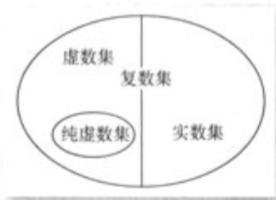
\includegraphics[width=0.7\textwidth]{docs/math/images/complex-1.png} 

\end{figure}



\subsection{复数的性质与运算}

\subsubsection{复数的几何意义}

我们知道了 $a+b\text{i}$ 这样类似的形式的数被称为复数,并且给出了定义和分类,我们还可以挖掘一下更深层的性质。

我们把所有实数都放在了数轴上,并且发现数轴上的点与实数一一对应。我们考虑对复数也这样处理。

首先我们定义\textbf{复数相等}:两个复数 $z_1=a+b\text{i},z_2=c+d\text{i}$ 是相等的,当且仅当 $a=c$ 且 $b=d$。

这么定义是十分自然的,在此不做过多解释。

也就是说,我们可以用唯一的有序实数对 $(a,b)$ 表示一个复数 $z=a+b\text{i}$。这样,联想到平面直角坐标系,我们可以发现\textbf{复数集与平面直角坐标系中的点集一一对应}。好了,我们找到了复数的一种几何意义。

那么这个平面直角坐标系就不再一般,因为平面直角坐标系中的点具有了特殊意义——表示一个复数,所以我们把这样的平面直角坐标系称为\textbf{复平面},$x$ 轴称为\textbf{实轴},$y$ 轴称为\textbf{虚轴}。我们进一步地说:\textbf{复数集与复平面内所有的点所构成的集合是一一对应的}。

我们考虑到学过的平面向量的知识,发现向量的坐标表示也是一个有序实数对 $(a,b)$,显然,复数 $z=a+b\text{i}$ 对应复平面内的点 $Z(a,b)$,那么它还对应平面向量 $\overrightarrow{OZ}=(a,b)$,于是我们又找到了复数的另一种几何意义:\textbf{复数集与复平面内的向量所构成的集合是一一对应的(实数 $0$ 与零向量对应)}。

于是,我们由向量的知识迁移到复数上来,定义\textbf{复数的模}就是复数所对应的向量的模。复数 $z=a+b\text{i}$ 的模 $|z|=\sqrt{a^2+b^2}$。

于是为了方便,我们常把复数 $z=a+b\text{i}$ 称为点 $Z$ 或向量 $\overrightarrow {OZ}$,并规定相等的向量表示同一个复数。

并且由向量的知识我们发现,虚数不可以比较大小(但是实数是可以的)。

\subsubsection{复数的运算}

\paragraph{复数的加法与减法}

我们规定,复数的加法规则如下:

设 $z_1=a+b\text{i},z_2=c+d\text{i}$,那么

$$
z_1+z_2=(a+c)+(b+d)\text{i}
$$

很明显,两个复数的和仍为复数。

考虑到向量的加法运算,我们发现复数的加法运算符合向量的加法运算法则,这同样证明了复数的几何意义的正确性。

同样可以验证,\textbf{复数的加法满足交换律和结合律}。即:

$$
z_1+z_2=z_2+z_1\\
(z_1+z_2)+z_3=z_1+(z_2+z_3)
$$

减法作为加法的逆运算,我们可以通过加法法则与复数相等的定义来推导出减法法则:

$$
z_1-z_2=(a-c)+(b-d)\text{i}
$$

这同样符合向量的减法运算。

\paragraph{复数的乘法与除法}

我们规定,复数的加法规则如下:

设 $z_1=a+b\text{i},z_2=c+d\text{i}$,那么

$$
\begin{aligned}
z_1z_2&=(a+b\text{i})(c+d\text{i})\\
&=ac+bc\text{i}+ad\text{i}+bd\text{i}^2\\
&=(ac-bd)+(bc+ad)\text{i}
\end{aligned}
$$

可以看出,两个复数相乘类似于两个多项式相乘,只需要把 $\text{i}^2$ 换成 $-1$,并将实部与虚部分别合并即可。

复数确实与多项式有关,因为复数域是实系数多项式环模掉 $x^2+1$ 生成的理想。(这句话不明白其实也没有关系)

复数的乘法与向量的向量积形式类似,是由于复数集是数环。

于是容易知道,\textbf{复数乘法满足交换律,结合律和对加法的分配律},即:

$$
z_1z_2=z_2z_1\\
(z_1z_2)z_3=z_1(z_2z_3)\\
z_1(z_2+z_3)=z_1z_2+z_1z_3
$$

由于满足运算律,我们可以发现实数域中的\textbf{乘法公式在复数域中同样适用}。

除法运算是乘法运算的逆运算,我们可以推导一下:

$$
\begin{aligned}
\frac{a+b\text{i}}{c+d\text{i}}&=\frac{(a+b\text{i})(c-d\text{i})}{(c+d\text{i})(c-d\text{i})}\\
&=\frac{ac+bd}{c^2+d^2}+\frac{bc-ad}{c^2+d^2}\text{i} &(c+d\text{i}\not =0)
\end{aligned}
$$

为了分母实数化,我们乘了一个 $c-d\text{i}$,这个式子很有意义。

我们定义,当两个虚数实部相等,虚部互为相反数时,这两个复数互为\textbf{共轭复数}。通常记 $z=a+b\text{i}$ 的共轭复数为 $\bar z=a-b\text{i}$。我们可以发现,两个复数互为共轭复数,那么它们\textbf{关于实轴对称}。

由于向量没有除法,这里不讨论与向量的关系。

\section{分段打表}

在学习之前请先学习  分块 。

打表大家都知道,就是在比赛时把答案都输出出来,然后开个数组,把答案直接存入数组里。于是你的代码时间复杂度就是 $O(1)$ 的了。

但是需要注意这个技巧只适用于类似输出某函数值类的问题。比如规定 $f(x)$ 为整数 $x$ 的二进制表示中 $1$ 的个数。输入一个正整数 $n$,输出 $\sum_{i=1}^nf^2(i)$。这样的话 $n$ 不大时,采用打表的方法可以做到 $O(1)$ 的复杂度。

注意到这个问题其实十分的简单,采用一般做法也可以做到 $O(n\log n)$ 的复杂度,但是 $n=10^9$?

还有一些时候,打出来的表十分大,如果对于每一个 $n$,都输出 $f(n)$ 的话,那么 MLE 之外,还有可能代码超过最大代码长度限制,导致编译前不通过(代码可能直接被 pass)。

我们考虑优化这个答案表,借用分块思想,我们设置一个合理的步长 $m$(这个步长一般视代码长度而定),对于第 $i$ 块,输出:

$$
\Large \sum_{k=\frac{n}{m}(i-1)+1}^{\frac{ni}{m}} f^2(k)
$$

的值。

然后输出答案时借用分块思想处理即可。

一般来说,这样的问题对于处理单个函数值 $f(x)$ 很快,但是需要大量函数值求和(求积或某些可以快速合并的操作),枚举会超出时间限制,在找不到标准做法的情况下,分段打表是一个不错的选择。

\subsubsection{注意事项}

\begin{enumerate}
\item 当上题中指数不是定值,但是范围较小,也可以考虑打表;
\item 上题是本人为了介绍分段打表口胡出来的,如已有此题纯属巧合。
\end{enumerate}

\subsubsection{例题}

\href{https://www.lydsy.com/JudgeOnline/problem.php?id=3798}{「BZOJ 3798」特殊的质数}:权限题……\sout{不过可以在各大 BZ 离线题库中看到。}

\href{https://www.zhihu.com/question/60674478/answer/180805562}{题意简述}:求 $[l,r]$ 区间内有多少个质数可以分解为两个正整数的平方和。—— via PoPoQQQ

\href{https://www.luogu.org/problem/show?pid=P1822}{「Luogu P1822」魔法指纹}:其实是一道暴搜,不过可以练练分段打表。


\section{莫比乌斯反演}

\subsection{简介}

莫比乌斯反演是数论中的重要内容。对于一些函数 $f(n)$,如果很难直接求出它的值,而容易求出其倍数和或约数和 $g(n)$,那么可以通过莫比乌斯反演简化运算,求得 $f(n)$ 的值。

开始学习莫比乌斯反演前,我们需要一些前置知识:\textbf{积性函数}、\textbf{Dirichlet 卷积}、\textbf{莫比乌斯函数}。

\hr

\subsection{积性函数}

\subsubsection{定义}

若 $\gcd(x,y)=1$ 且 $f(xy)=f(x)f(y)$,则 $f(n)$ 为积性函数。

\subsubsection{性质}

若 $f(x)$ 和 $g(x)$ 均为积性函数,则以下函数也为积性函数:

$$
\begin{aligned}
h(x)&=f(x^p)\\
h(x)&=f^p(x)\\
h(x)&=f(x)g(x)\\
h(x)&=\sum_{d\mid x}f(d)g(\frac{x}{d})
\end{aligned}
$$

\subsubsection{例子}

$$
\qquad\begin{aligned}
\text{约数个数函数}&d(n)=\displaystyle\sum_{d\mid n}1\\
\text{约数和函数}&\displaystyle\sigma(n)=\sum_{d\mid n}d\\
\text{约数 $k$ 次幂函数}&\displaystyle\sigma_k(n)=\sum_{d\mid n}d^k\\
\text{欧拉函数}&\displaystyle\varphi(n)=\sum_{i=1}^n [\gcd(i,n)=1]\\
\text{莫比乌斯函数}&\displaystyle\mu(n)=
\begin{cases}
1 & n=1\\
(-1)^k &c_{1,2,\cdots,k}=1\quad(n=\displaystyle\prod_{i=1}^k {p_i}^{c_i})\\
0 & c_i>1
\end{cases}
\end{aligned}
$$

\hr

\subsection{Dirichlet 卷积}

\subsubsection{定义}

定义两个数论函数 $f,g$ 的 $\text{Dirichlet}$ 卷积为

$$
(f*g)(n)=\sum_{d\mid n}f(d)g(\frac{n}{d})
$$

\subsubsection{性质}

$\text{Dirichlet}$ 卷积满足交换律和结合律。

其中 $\varepsilon$ 为 $\text{Dirichlet}$ 卷积的单位元(任何函数卷 $\varepsilon$ 都为其本身)

\subsubsection{例子}

$$
\begin{aligned}
\varepsilon=\mu*1&\Leftrightarrow\varepsilon(n)=\sum_{d\mid n}\mu(d)\\
d=1*1&\Leftrightarrow d(n)=\sum_{d\mid n}1\\
\sigma=d*1&\Leftrightarrow\varepsilon(n)=\sum_{d\mid n}d\\
\varphi=\mu*\text{ID}&\Leftrightarrow\varphi(n)=\sum_{d\mid n}d\cdot\mu(\frac{n}{d})
\end{aligned}
$$

\hr

\subsection{莫比乌斯函数}

\subsubsection{定义}

$\mu$ 为莫比乌斯函数

\subsubsection{性质}

莫比乌斯函数不但是积性函数,还有如下性质:

$$
\mu(n)=
\begin{cases}
1&n=1\\
0&n\text{ 含有平方因子}\\
(-1)^k&k\text{ 为 }n\text{ 的本质不同质因子个数}\\
\end{cases}
$$

\subsubsection{证明}

$$
\varepsilon(n)=
\begin{cases}
1&n=1\\
0&n\neq 1\\
\end{cases}
$$

其中 $\displaystyle\varepsilon(n)=\sum_{d\mid n}\mu(d)$ 即 $\varepsilon=\mu*1$

设 $\displaystyle n=\prod_{i=1}^k{p_i}^{c_i},n'=\prod_{i=1}^k p_i$

那么 $\displaystyle\sum_{d\mid n}\mu(d)=\sum_{d\mid n'}\mu(d)=\sum_{i=0}^k C_k^i\cdot(-1)^k$

根据二项式定理,易知该式子的值在 $k=0$ 即 $n=1$ 时值为 $1$ 否则为 $0$,这也同时证明了 $\displaystyle\sum_{d\mid n}\mu(d)=[n=1]$

\subsubsection{补充结论}

反演结论:$\displaystyle [gcd(i,j)=1] \Leftrightarrow\sum_{d\mid\gcd(i,j)}\mu(d)$

\begin{itemize}
\item \textbf{直接推导}:如果看懂了上一个结论,这个结论稍加思考便可以推出:如果 $\gcd(i,j)=1$ 的话,那么代表着我们按上个结论中枚举的那个 $n$ 是 $1$,也就是式子的值是 $1$,反之,有一个与 $[\gcd(i,j)=1]$ 相同的值:$0$
\item \textbf{利用 $\varepsilon$ 函数}:根据上一结论,$[\gcd(i,j)=1]\Rightarrow \varepsilon(\gcd(i,j))$,将 $\varepsilon$ 展开即可。
\end{itemize}

\subsubsection{线性筛}

由于 $\mu$ 函数为积性函数,因此可以线性筛莫比乌斯函数(线性筛基本可以求所有的积性函数,尽管方法不尽相同)。

\textbf{代码}:

\begin{cppcode}
void getMu() {
  mu[1] = 1;
  for (int i = 2; i <= n; ++i) {
    if (!flg[i]) p[++tot] = i, mu[i] = -1;
    for (int j = 1; j <= tot && i * p[j] <= n; ++j) {
      flg[i * p[j]] = 1;
      if (i % p[j] == 0) {
        mu[i * p[j]] = 0;
        break;
      }
      mu[i * p[j]] = -mu[i];
    }
  }
}
\end{cppcode}

\subsubsection{拓展}

证明

$$
\varphi*1=\text{ID}\text{(ID 函数即 } f(x)=x\text{)}
$$

将 $n$ 分解质因数:$\displaystyle n=\prod_{i=1}^k {p_i}^{c_i}$

首先,因为 $\varphi$ 是积性函数,故只要证明当 $n'=p^c$ 时 $\displaystyle\varphi*1=\sum_{d\mid n'}\varphi(\frac{n'}{d})=\text{ID}$ 成立即可。

因为 $p$ 是质数,于是 $d=p^0,p^1,p^2,\cdots,p^c$

易知如下过程:

$$
\begin{aligned}
\varphi*1&=\sum_{d\mid n}\varphi(\frac{n}{d})\\
&=\sum_{i=0}^c\varphi(p^i)\\
&=1+p^0\cdot(p-1)+p^1\cdot(p-1)+\cdots+p^{c-1}\cdot(p-1)\\
&=p^c\\
&=\text{ID}\\
\end{aligned}
$$

该式子两侧同时卷 $\mu$ 可得 $\displaystyle\varphi(n)=\sum_{d\mid n}d\cdot\mu(\frac{n}{d})$

\hr

\subsection{莫比乌斯反演}

\subsubsection{公式}

设 $f(n),g(n)$ 为两个数论函数。

如果有

$$
f(n)=\sum_{d\mid n}g(d)
$$

那么有

$$
g(n)=\sum_{d\mid n}\mu(d)f(\frac{n}{d})
$$

\subsubsection{证明}

\begin{itemize}
\item \textbf{暴力计算}:
\end{itemize}

$$
\sum_{d\mid n}\mu(d)f(\frac{n}{d})=\sum_{d\mid n}\mu(d)\sum_{k\mid \frac{n}{d}}g(k)=\sum_{k\mid n}g(k)\sum_{d\mid \frac{n}{k}}\mu(d)=g(n)
$$

用 $\displaystyle\sum_{d\mid n}g(d)$ 来替换 $f(\dfrac{n}{d})$,再变换求和顺序。最后一步转为的依据:$\displaystyle\sum_{d\mid n}\mu(d)=[n=1]$,因此在 $\dfrac{n}{k}=1$ 时第二个和式的值才为 $1$。此时 $n=k$,故原式等价于 $\displaystyle\sum_{k\mid n}[n=k]\cdot g(k)=g(n)$

\begin{itemize}
\item \textbf{运用卷积}:
\end{itemize}

原问题为:已知 $f=g*1$,证明 $g=f*\mu$

易知如下转化:$f*\mu=g*1*\mu\Rightarrow f*\mu=g$(其中 $1*\mu=\varepsilon$)

\hr

\subsection{问题形式}

\subsubsection{\href{https://www.lydsy.com/JudgeOnline/problem.php?id=2301}{「HAOI 2011」Problem b}}

求值(多组数据)

$$
\sum_{i=x}^{n}\sum_{j=y}^{m}[\gcd(i,j)=k]\qquad (1\leqslant T,x,y,n,m,k\leqslant 5\times 10^4)
$$

根据容斥原理,原式可以分成 $4$ 块来处理,每一块的式子都为

$$
\sum_{i=1}^{n}\sum_{j=1}^{m}[\gcd(i,j)=k]
$$

考虑化简该式子

$$
\sum_{i=1}^{\lfloor\frac{n}{k}\rfloor}\sum_{j=1}^{\lfloor\frac{m}{k}\rfloor}[\gcd(i,j)=1]
$$

因为 $\gcd(i,j)=1$ 时对答案才用贡献,于是我们可以将其替换为 $\varepsilon(\gcd(i,j))$($\varepsilon(n)$ 当且仅当 $n=1$ 时值为 $1$ 否则为 $0$ ),故原式化为

$$
\sum_{i=1}^{\lfloor\frac{n}{k}\rfloor}\sum_{j=1}^{\lfloor\frac{m}{k}\rfloor}\varepsilon(\gcd(i,j))
$$

将 $\varepsilon$ 函数展开得到

$$
\displaystyle\sum_{i=1}^{\lfloor\frac{n}{k}\rfloor}\sum_{j=1}^{\lfloor\frac{m}{k}\rfloor}\sum_{d\mid  \gcd(i,j)}\mu(d)
$$

变换求和顺序,先枚举 $d\mid gcd(i,j)$ 可得

$$
\displaystyle\sum_{d=1}^{\lfloor\frac{n}{k}\rfloor}\mu(d)\sum_{i=1}^{\lfloor\frac{n}{k}\rfloor}d\mid i\sum_{j=1}^{\lfloor\frac{m}{k}\rfloor}d\mid j
$$

(其中 $d\mid i$ 表示 $i$ 是 $d$ 的倍数时对答案有 $1$ 的贡献)

易知 $1\sim\lfloor\dfrac{n}{k}\rfloor$ 中 $d$ 的倍数有 $\lfloor\dfrac{n}{kd}\rfloor$ 个,故原式化为

$$
\displaystyle\sum_{d=1}^{\lfloor\frac{n}{k}\rfloor}\mu(d) \lfloor\frac{n}{kd}\rfloor\lfloor\frac{m}{kd}\rfloor
$$

很显然,式子可以数论分块求解(注意:过程中默认 $n\leqslant m$)。

\textbf{时间复杂度}:$\Theta(N+T\sqrt{n})$

\textbf{代码}:

\begin{cppcode}
#include <algorithm>
#include <cstdio>
const int N = 50000;
int mu[N + 5], p[N + 5];
bool flg[N + 5];
void init() {
  int tot = 0;
  mu[1] = 1;
  for (int i = 2; i <= N; ++i) {
    if (!flg[i]) {
      p[++tot] = i;
      mu[i] = -1;
    }
    for (int j = 1; j <= tot && i * p[j] <= N; ++j) {
      flg[i * p[j]] = 1;
      if (i % p[j] == 0) {
        mu[i * p[j]] = 0;
        break;
      }
      mu[i * p[j]] = -mu[i];
    }
  }
  for (int i = 1; i <= N; ++i) mu[i] += mu[i - 1];
}
int solve(int n, int m) {
  int res = 0;
  for (int i = 1, j; i <= std::min(n, m); i = j + 1) {
    j = std::min(n / (n / i), m / (m / i));
    res += (mu[j] - mu[i - 1]) * (n / i) * (m / i);
  }
  return res;
}
int main() {
  int T, a, b, c, d, k;
  init();
  for (scanf("%d", &T); T; --T) {
    scanf("%d%d%d%d%d", &a, &b, &c, &d, &k);
    printf("%d\n", solve(b / k, d / k) - solve(b / k, (c - 1) / k) -
                       solve((a - 1) / k, d / k) +
                       solve((a - 1) / k, (c - 1) / k));
  }
  return 0;
}
\end{cppcode}

\subsubsection{\href{https://www.luogu.org/problemnew/show/SP5971}{「SPOJ 5971」LCMSUM}}

求值(多组数据)

$$
\sum_{i=1}^n \text{lcm}(i,n)\qquad (1\leqslant T\leqslant 3\times 10^5,1\leqslant n\leqslant 10^6)
$$

易得原式即

$$
\sum_{i=1}^n \frac{i\cdot n}{\gcd(i,n)}
$$

根据 $\gcd(a,n)=1$ 时一定有 $\gcd(n-a,n)=1$ ,可将原式化为

$$
\frac{1}{2}\cdot(\sum_{i=1}^{n-1}\frac{i\cdot n}{\gcd(i,n)}+\sum_{i=n-1}^{1}\frac{i\cdot n}{\gcd(i,n)})+n
$$

上述式子中括号内的两个 $\sum$ 对应的项相等,故又可以化为

$$
\frac{1}{2}\cdot \sum_{i=1}^{n-1}\frac{n^2}{\gcd(i,n)}+n
$$

可以将相同的 $\gcd(i,n)$ 合并在一起计算,故只需要统计 $\gcd(i,n)=d$ 的个数。当 $\gcd(i,n)=d$ 时,$\displaystyle\gcd(\frac{i}{d},\frac{n}{d})=1$,所以 $\gcd(i,n)=d$ 的个数有 $\displaystyle\varphi(\frac{n}{d})$ 个。

故答案为

$$
 \frac{1}{2}\cdot\sum_{d\mid n}\frac{n^2\cdot\varphi(\frac{n}{d})}{d}+n
$$

变换求和顺序,设 $\displaystyle d'=\frac{n}{d}$,式子化为

$$
\frac{1}{2}n\cdot\sum_{d'\mid n}d'\cdot\varphi(d')+n
$$

设 $\displaystyle \text{g}(n)=\sum_{d\mid n} d\cdot\varphi(d)$,已知 $\text{g}$ 为积性函数,于是可以 $\Theta(n)$ 预处理。最后枚举 $d$,统计贡献即可。

\textbf{时间复杂度}:$\Theta(n\log n)$

\textbf{代码}:

\begin{cppcode}
#include <cstdio>
const int N = 1000000;
int tot, p[N + 5], phi[N + 5];
long long ans[N + 5];
bool flg[N + 5];

void solve() {
  phi[1] = 1;
  for (int i = 2; i <= N; ++i) {
    if (!flg[i]) p[++tot] = i, phi[i] = i - 1;
    for (int j = 1; j <= tot && i * p[j] <= N; ++j) {
      flg[i * p[j]] = 1;
      if (i % p[j] == 0) {
        phi[i * p[j]] = phi[i] * p[j];
        break;
      }
      phi[i * p[j]] = phi[i] * (p[j] - 1);
    }
  }
  for (int i = 1; i <= N; ++i) {
    for (int j = 1; i * j <= N; ++j) {
      ans[i * j] += 1LL * j * phi[j] / 2;
    }
  }
  for (int i = 1; i <= N; ++i) ans[i] = 1LL * i * ans[i] + i;
}
int main() {
  int T, n;
  solve();
  for (scanf("%d", &T); T; --T) {
    scanf("%d", &n);
    printf("%lld\n", ans[n]);
  }
  return 0;
}
\end{cppcode}

\subsubsection{\href{https://www.lydsy.com/JudgeOnline/problem.php?id=2154}{「BZOJ 2154」Crash 的数字表格}}

求值(对 $20101009$ 取模)

$$
\sum_{i=1}^n\sum_{j=1}^m\text{lcm}(i,j)\qquad (n,m\leqslant 10^7)
$$

易知原式等价于

$$
\sum_{i=1}^n\sum_{j=1}^m\frac{i\cdot j}{\gcd(i,j)}
$$

枚举最大公因数 $d$,显然两个数除以 $d$ 得到的数互质

$$
\sum_{i=1}^n\sum_{j=1}^m\sum_{d\mid i,d\mid j,\gcd(\frac{i}{d},\frac{j}{d})=1}\frac{i\cdot j}{d}
$$

非常经典的 $\gcd$ 式子的化法

$$
\sum_{d=1}^n d\cdot\sum_{i=1}^{\lfloor\frac{n}{d}\rfloor}\sum_{j=1}^{\lfloor\frac{m}{d}\rfloor}[\gcd(i,j)=1]\ i\cdot j
$$

后半段式子中,出现了互质数对之积的和,为了让式子更简洁就把它拿出来单独计算。于是我们记

$$
\text{sum}(n,m)=\sum_{i=1}^n\sum_{j=1}^m [\gcd(i,j)=1]\  i\cdot j
$$

接下来对 $\text{sum}(n,m)$ 进行化简。首先枚举约数,并将 $[\gcd(i,j)=1]$ 表示为 $\varepsilon(\gcd(i,j))$

$$
\sum_{d=1}^n\sum_{d\mid i}^n\sum_{d\mid j}^m\mu(d)\cdot i\cdot j
$$

设 $i=i'\cdot d$,$j=j'\cdot d$,显然式子可以变为

$$
\sum_{d=1}^n\mu(d)\cdot d^2\cdot\sum_{i=1}^{\lfloor\frac{n}{d}\rfloor}\sum_{j=1}^{\lfloor\frac{m}{d}\rfloor}i\cdot j
$$

观察上式,前半段可以预处理前缀和;后半段又是一个范围内数对之和,记

$$
g(n,m)=\sum_{i=1}^n\sum_{j=1}^m i\cdot j=\frac{n\cdot(n+1)}{2}\times\frac{m\cdot(m+1)}{2}
$$

可以 $\Theta(1)$ 求解

至此

$$
\text{sum}(n,m)=\sum_{d=1}^n\mu(d)\cdot d^2\cdot g(\lfloor\frac{n}{d}\rfloor,\lfloor\frac{m}{d}\rfloor)
$$

我们可以 $\lfloor\frac{n}{\lfloor\frac{n}{d}\rfloor}\rfloor$ 数论分块求解 $\text{sum}(n,m)$ 函数。

在求出 $\text{sum}(n,m)$ 后,回到定义 $\text{sum}$ 的地方,可得原式为

$$
\sum_{d=1}^n d\cdot\text{sum}(\lfloor\frac{n}{d}\rfloor,\lfloor\frac{m}{d}\rfloor)
$$

可见这又是一个可以数论分块求解的式子!

本题除了推式子比较复杂、代码细节较多之外,是一道很好的莫比乌斯反演练习题!(上述过程中,默认 $n\leqslant m$)

\textbf{时间复杂度}:$\Theta(n+m)$(两次数论分块)

\textbf{代码}:

\begin{cppcode}
#include <algorithm>
#include <cstdio>
using std::min;

const int N = 1e7;
const int mod = 20101009;
int n, m, mu[N + 5], p[N / 10 + 5], sum[N + 5];
bool flg[N + 5];

void init() {
  mu[1] = 1;
  int tot = 0, k = min(n, m);
  for (int i = 2; i <= k; ++i) {
    if (!flg[i]) p[++tot] = i, mu[i] = -1;
    for (int j = 1; j <= tot && i * p[j] <= k; ++j) {
      flg[i * p[j]] = 1;
      if (i % p[j] == 0) {
        mu[i * p[j]] = 0;
        break;
      }
      mu[i * p[j]] = -mu[i];
    }
  }
  for (int i = 1; i <= k; ++i)
    sum[i] = (sum[i - 1] + 1LL * i * i % mod * (mu[i] + mod)) % mod;
}
int Sum(int x, int y) {
  return (1LL * x * (x + 1) / 2 % mod) * (1LL * y * (y + 1) / 2 % mod) % mod;
}
int func(int x, int y) {
  int res = 0;
  for (int i = 1, j; i <= min(x, y); i = j + 1) {
    j = min(x / (x / i), y / (y / i));
    res = (res + 1LL * (sum[j] - sum[i - 1] + mod) * Sum(x / i, y / i) % mod) %
          mod;
  }
  return res;
}
int solve(int x, int y) {
  int res = 0;
  for (int i = 1, j; i <= min(x, y); i = j + 1) {
    j = min(x / (x / i), y / (y / i));
    res = (res +
           1LL * (j - i + 1) * (i + j) / 2 % mod * func(x / i, y / i) % mod) %
          mod;
  }
  return res;
}
int main() {
  scanf("%d%d", &n, &m);
  init();
  printf("%d\n", solve(n, m));
}
\end{cppcode}

\begin{QUOTE}{}{}
本文部分内容引用于 \href{https://algocode.net}{algocode 算法博客},特别鸣谢!
\end{QUOTE}

\section{杜教筛}

在数论题目中,常常需要根据一些 \textbf{ 积性函数 } 的性质,求出一些式子的值。

\textbf{ 积性函数 } : 对于所有互质的 $a$ 和 $b$ ,总有 $f(ab)=f(a)f(b)$ ,则称 $f(x)$ 为积性函数。

常见的积性函数有:

$d(x)=\sum_{i|n} 1$

$\sigma(x)=\sum_{i|n} i$

$\varphi(x)=\sum_{i=1}^x 1[gcd(x,i)=1]$

$\mu(x)=\begin{cases}1&\text{n=1}\\(-1)^k& \ \prod_{i=1}^k q_i=1\\0 &\ \max\{q_i\}>1\end{cases}$

积性函数有如下性质:

若 $f(x)$ , $g(x)$ 为积性函数,则

$h(x)=f(x^p)$ 

$h(x)=f^p(x)$

$h(x)=f(x)g(x)$

$h(x)=\sum_{d|x} f(d)g(\frac x d)$

中的 $h(x)$ 也为积性函数。

在莫比乌斯反演的题目中,往往要求出一些数论函数的前缀和,利用 \textbf{ 杜教筛 } 可以快速求出这些前缀和。 

\begin{NOTE}{例题 \href{https://www.luogu.org/problemnew/show/P4213}{P4213 【模板】杜教筛( Sum ) }}{}

\end{NOTE}


题目大意: 求 $S_1(n)= \sum_{i=1}^n \mu(i)$ 和 $S_2(n)= \sum_{i=1}^n \varphi(i)$  的值, $n\le 2^{31} -1$ 。

由 \textbf{ 狄利克雷卷积 } ,我们知道:

$\because \epsilon =\mu * 1$ ( $\epsilon(n)=~[n=1]$ ) 

$\therefore \epsilon (n)=\sum_{d|n} \mu(d)$ 

$S_1(n)=\sum_{i=1}^n \epsilon (i)-\sum_{i=2}^n S_1(\lfloor \frac n i \rfloor)$

$= 1-\sum_{i=2}^n S_1(\lfloor \frac n i \rfloor)$

观察到 $\lfloor \frac n i \rfloor$ 最多只有 $O(\sqrt n)$ 种取值,我们就可以应用 \textbf{ 整除分块 } (或称数论分块)来计算每一项的值了。 

直接计算的时间复杂度为 $O(n^{\frac 3 4})$ 。考虑先线性筛预处理出前 $n^{\frac 2 3}$ 项,剩余部分的时间复杂度为

$O(\int_{0}^{n^{\frac 1 3}} \sqrt{\frac{n}{x}} ~ dx)=O(n^{\frac 2 3})$ 

对于较大的值,需要用 \texttt{map} 存下其对应的值,方便以后使用时直接使用之前计算的结果。

当然也可以用杜教筛求出 $\varphi (x)$ 的前缀和,但是更好的方法是应用莫比乌斯反演:

$\sum_{i=1}^n \sum_{j=1}^n 1[gcd(i,j)=1]=\sum_{i=1}^n \sum_{j=1}^n \sum_{d|i,d|j} \mu(d)$

$=\sum_{d=1}^n \mu(d) {\lfloor \frac n d \rfloor}^2$

由于题目所求的是 $\sum_{i=1}^n \sum_{j=1}^i 1[gcd(i,j)=1]$ ,所以我们排除掉 $i=1,j=1$ 的情况,并将结果除以 $2$ 即可。 

观察到,只需求出莫比乌斯函数的前缀和,就可以快速计算出欧拉函数的前缀和了。时间复杂度 $O(n^{\frac 2 3})$ 。 

给出一种代码实现:

\begin{cppcode}
#include <algorithm>
#include <cstdio>
#include <cstring>
#include <map>
using namespace std;
const int maxn = 2000010;
typedef long long ll;
ll T, n, pri[maxn], cur, mu[maxn], sum_mu[maxn];
bool vis[maxn];
map<ll, ll> mp_mu;
ll S_mu(ll x) {
  if (x < maxn) return sum_mu[x];
  if (mp_mu[x]) return mp_mu[x];
  ll ret = 1ll;
  for (ll i = 2, j; i <= x; i = j + 1) {
    j = x / (x / i);
    ret -= S_mu(x / i) * (j - i + 1);
  }
  return mp_mu[x] = ret;
}
ll S_phi(ll x) {
  ll ret = 0ll;
  for (ll i = 1, j; i <= x; i = j + 1) {
    j = x / (x / i);
    ret += (S_mu(j) - S_mu(i - 1)) * (x / i) * (x / i);
  }
  return ((ret - 1) >> 1) + 1;
}
int main() {
  scanf("%lld", &T);
  mu[1] = 1;
  for (int i = 2; i < maxn; i++) {
    if (!vis[i]) {
      pri[++cur] = i;
      mu[i] = -1;
    }
    for (int j = 1; j <= cur && i * pri[j] < maxn; j++) {
      vis[i * pri[j]] = true;
      if (i % pri[j])
        mu[i * pri[j]] = -mu[i];
      else {
        mu[i * pri[j]] = 0;
        break;
      }
    }
  }
  for (int i = 1; i < maxn; i++) sum_mu[i] = sum_mu[i - 1] + mu[i];
  while (T--) {
    scanf("%lld", &n);
    printf("%lld %lld\n", S_phi(n), S_mu(n));
  }
  return 0;
}
\end{cppcode}

\section{线性基}



  \section{多项式部分简介}
  


  \section{拉格朗日插值}
  
\begin{NOTE}{例题 \href{https://www.luogu.org/problemnew/show/P4781}{洛谷 P4781 【模板】拉格朗日插值}}{}

\end{NOTE}


\subsubsection{题目大意}

给出 $n$ 个点 $P_i(x_i,y_i)$ ,将过这 $n$ 个点的最多 $n-1$ 次的多项式记为 $f(x)$ ,求 $f(k)$ 的值。

\subsubsection{方法 1:差分法}

差分法适用于 $x_i=i$ 的情况。

如,用差分法求 $f(x)=\sum_{i=1}^{x} i^2$ 的多项式形式。

\begin{minted}{text}
1   5   14   30   55   91
  4   9    16   25   36
    5   7     9   11
      2    2    2
\end{minted}

第一行为 $f(x)$ 的连续的前几项;若上面一行有 $n$ 个值,下面一行有 $n-1$ 个值,每个值为上面对应的相邻两项的差。观察到,如果这样操作的次数足够多(前提是 $f(x)$ 为多项式),每次总会返回一个定值,可以利用这个定值求出 $f(x)$ 的每一项的系数,然后即可将 $k$ 代入多项式中求解。如上例中可求出 $f(x)=\frac 1 3 n^3+\frac 1 2 n^2+\frac 1 6 n$ 。时间复杂度为 $O(n^2)$ ,对给出的点的限制性较强。

\subsubsection{方法 2:高斯消元}

使用 \textbf{ 待定系数法 } 。设 $f(x)=\sum_{i=0}^{n-1} a_ix^i$将每个 $x_i$ 代入 $f(x)$ ,有 $f(x_i)=y_i$ ,这样就可以得到一个由 $n$ 条 $n$ 元 $1$ 次方程所组成的方程组,然后使用 \textbf{ 高斯消元 } 求出每一项 $a_i$ ,然后将 $k$ 代入求值。

如果您不知道什么是高斯消元,请看 \href{https://www.luogu.org/problemnew/show/P3389}{luogu P3389 高斯消元法} 。

时间复杂度 $O(n^3)$ ,对给出点的坐标无要求。

\subsubsection{方法 3: 拉格朗日差值法}

考虑将每个点做一个对于 $x$ 轴的垂线,设垂足为 $H_i(x_i,0)$ 。

\begin{figure}[htbp]
\centering
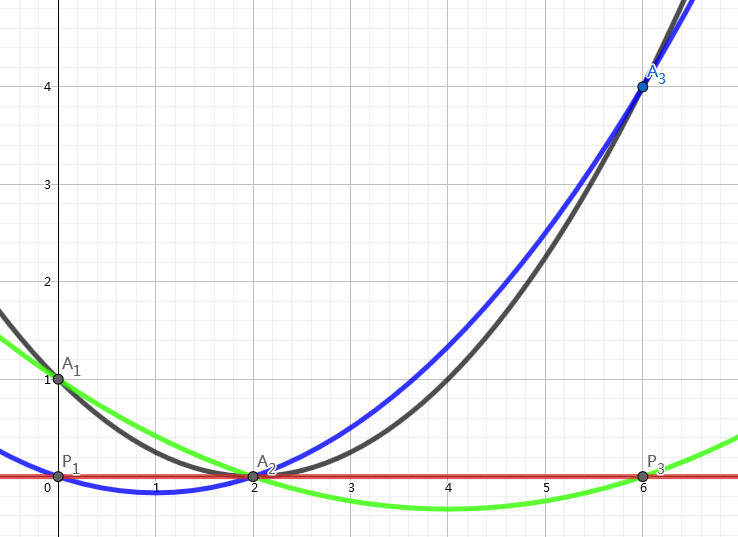
\includegraphics[width=0.7\textwidth]{docs/math/images/lagrange-poly-1.png} 

\end{figure}

如上图所示,黑线等于蓝线加绿线加红线。每次我们选择 $1$ 个 $P_i$ ,并选择其他的 $H_j[j\neq i]$ ,做一条过这些点的一条至多 $n-1$ 次的线。由于有 $n-2$ 个点都在 $x$ 轴上,我们知道这条线的解析式一定是形如 $g_i(x)=y_i\times (\prod_{i=1}^{n} (x-x_i)[i\neq x])$ 的形式。

最后将所有的 $g(x)$ 相加,即 $f(x)=sum_{i=1}^{n}g_i(x)$ 。因为对于每个点 $P_i$ ,都只有一条函数经过 $P_i$ ,其余都经过 $H_i$ ,这一项的系数是 $0$ ,所以最后的和函数总是过所有 $n$ 个点的。

公式整理得:

$f(x)=\sum_{i=1}^{n} y_i\times(\prod_{j\neq i }\frac{x-x_j}{x_i-x_j})$

如果要将每一项都算出来,时间复杂度仍是 $O(n^2)$ 的,但是本题中只用求出 $f(k)$ 的值,所以只需将 $k$ 代入进式子里得:

$Ans=\sum_{i=1}^{n} y_i\times(\prod_{j\neq i }\frac{k-x_j}{x_i-x_j})$

本题中,还需要求解逆元。如果先分别计算出分子和分母,在计算分母的逆元,乘上分子,累加进最后的答案,时间复杂度的瓶颈就不会在求逆元上,时间复杂度为 $O(n^2)$ 。

\subsubsection{代码实现}

\begin{cppcode}
#include <algorithm>
#include <cstdio>
#include <cstring>
using namespace std;
const int maxn = 2010;
typedef long long ll;
ll mod = 998244353;
ll n, k, x[maxn], y[maxn], ans, s1, s2;
ll powmod(ll a, ll x) {
  ll ret = 1ll, nww = a;
  while (x) {
    if (x & 1) ret = ret * nww % mod;
    nww = nww * nww % mod;
    x >>= 1;
  }
  return ret;
}
ll inv(ll x) { return powmod(x, mod - 2); }
int main() {
  scanf("%lld%lld", &n, &k);
  for (int i = 1; i <= n; i++) scanf("%lld%lld", x + i, y + i);
  for (int i = 1; i <= n; i++) {
    s1 = y[i] % mod;
    s2 = 1ll;
    for (int j = 1; j <= n; j++)
      if (i != j)
        s1 = s1 * (k - x[j]) % mod, s2 = s2 * ((x[i] - x[j] % mod) % mod) % mod;
    ans += s1 * inv(s2) % mod;
    ans = (ans + mod) % mod;
  }
  printf("%lld\n", ans);
  return 0;
}
\end{cppcode}

  \section{快速傅里叶变换}
  
(本文转载自 \href{https://zhuanlan.zhihu.com/c_1005817911142838272}{桃酱的算法笔记},原文戳 \href{https://zhuanlan.zhihu.com/p/41867199}{链接},已获得作者授权)

一直想学 FFT,之前牛客的多小有一道组合数学就用 FFT 写的,而且当时还傻乎乎的用唯一分解定理,但是自己好久没静下心学什么了,而且自己的数学功底又不好,导致一直学不会。看了很多人的博客也没看明白,尤其是原根。在我看了几十篇博客之后终于看懂了。。。所以想写一篇能够让大多数人都看得懂的教程。花费时间 3 天终于写完啦\sout{}\textbackslash{}\textasciitilde{}\textasciitilde{}

另外,本文 FFT 部分的代码实现全部参考 kuangbin 的模板(2018.7 更新)资源地址如下

\url{https://download.csdn.net/download/qq_37136305/10562410}

NTT 部分代码参考 CSDN 上的模板代码附网址,感谢博主!

你搜索这个关键词就已经知道这一是个数学的东西了。只想学会用很简单,但是这远远不够。所以在看这个博客之前应该先学一下  复数  的基本知识。

好了下面进入正文。

\subsection{DFT IDFT FFT 官方定义?}

\begin{QUOTE}{}{}
离散傅里叶变换(Discrete Fourier Transform,缩写为 DFT),是傅里叶变换在时域和频域上都呈离散的形式,将信号的时域采样变换为其 DTFT 的频域采样。



FFT 是一种 DFT 的高效算法,称为快速傅立叶变换(fast Fourier transform)。 ——百度百科
\end{QUOTE}

在百度百科上能找到 DFT 和 FFT 这两个定义。正如定义,FFT 和 DFT 实际上按照结果来看的话是一样的,但是 FFT 比较快的计算 DFT 和IDFT(离散反傅里叶变换)。

快速数论变换 (NTT) 是快速傅里叶变换(FFT)在数论基础上的实现。

是不是有点迷 QAQ?既然是官方定义那肯定不能让你看懂才对嘛~下面我们一一解释~

\subsection{为什么要使用 FFT?}

我们在这里引入一个例子:求多项式乘积的朴素算法。

大家平时求 $f(x)=a_1x^2+b_1x+c_1$ 与 $g(x) = a_2x^2+b_2x+c_2$ 的乘积时候,是怎么进行的呢?

我们令

$$
K(x) = f(x)  \times  g(x) = a_1x^2 \times a_2x^2+a_1x^2 \times b_2x+a_1x^2 \times c_2+b_1x \times b_2x^2+b_1x \times b_2x+b_1x \times c_2+c_1 \times a_2x^2+c_1 \times b_2x+c_1 \times c_2
$$

那么很显然我们进行了 9 次运算,复杂度是 $O(n^2)$ (具体代码实现不再展开)

但是如果数字足够大呢?比如 100000?那朴素算法可太慢啦 (;′⌒),

\subsection{什么是 FFT}

FFT,即为快速傅氏变换,是离散傅氏变换的快速算法,它是根据离散傅氏变换的奇、偶、虚、实等特性,对离散傅立叶变换的算法进行改进获得的。它对傅氏变换的理论并没有新的发现,但是对于在计算机系统或者说数字系统中应用离散傅立叶变换,可以说是进了一大步。——360 百科

如果上一个例子用朴素算法太慢啦!所以我们要用 FFT 进行优化,复杂度会降为 $O(nlogn)$

\subsubsection{多项式的系数表示法与点值表示法}

一个多项式,我们可以怎样来表示呢?

系数表示法就是用一个多项式的各个项系数来表达这个多项式。比如:

$$
f(x) = a_1x^2+b_1x+c_1 \Leftrightarrow f(x) = \{a_1, b_1, c_1\}
$$

点值表示法是把这个多项式看成一个函数,从上面选取 $n+1$ 个点,从而利用这 $n+1$ 个点来唯一的表示这个函数。为什么用 $n+1$ 个点就能唯一的表示这个函数了呢?想一下高斯消元法,两点确定一条直线。再来一个点,能确定这个直线中的另一个参数,那么也就是说 $n+1$ 个点能确定 $n$ 个参数(不考虑倍数点之类的没用点)。如下:

$$
f_1(x) = y_1 = a_0 + a_1x_1+a_2x_1^2+a_3x_1^3+ \cdots + a_nx_1^n
$$

$$
f_2(x) = y_2 = a_0 + a_1x_2+a_2x_2^2+a_3x_2^3+ \cdots + a_nx_2^n
$$

$$
f_3(x) = y_3 = a_0 + a_1x_3+a_2x_3^2+a_3x_3^3+ \cdots + a_nx_3^n
$$

$$
f_4(x) = y_4 = a_0 + a_1x_4+a_2x_4^2+a_3x_4^3+ \cdots + a_nx_4^n
$$

$$
f_5(x) = y_5 = a_0 + a_1x_5+a_2x_5^2+a_3x_5^3+ \cdots + a_nx_5^n
$$

$$
\cdots
$$

$$
f_n(x) = y_n = a_0 + a_1x_m+a_2x_m^2+a_3x_m^3+ \cdots + a_nx_m^n
$$

一个非常通俗易懂的解释:

多项式由系数表示法转为点值表示法的过程,就成为 DFT;

相对地,把一个多项式的点值表示法转化为系数表示法的过程,就是 IDFT。

而 FFT 就是通过取某些特殊的 $x$ 的点值来加速 DFT 和 FFT 的过程。

\subsubsection{复数的引入}

复数分为实数和虚数。实数就是我们日常最常用的有理数和无理数。大家记得我们在开始学平方的时候,老师会说所有数的平方大于等于 $0$ 对不对,那么虚数就引入了。虚数一般用 $i$ 表示,对于虚数 $i$,有 $i=\sqrt{-1}$

。另外,$i$ 对于虚数的意义,与 $1$ 对于实数的意义是一样的。如果我说得不够明确,你可以看下面我引用的百科说明。

\begin{QUOTE}{}{}
在数学中,虚数就是形如 $a+b \times i$ 的数,其中 $a,b$ 是实数,且 $b \neq 0$,$i^2 = - 1$。虚数这个名词是 17 世纪著名数学家笛卡尔创立,因为当时的观念认为这是真实不存在的数字。后来发现虚数 $a+b \times i$ 的实部 $a$ 可对应平面上的横轴,虚部 $b$ 与对应平面上的纵轴,这样虚数 $a+b \times i$ 可与平面内的点 $(a,b)$ 对应。



可以将虚数 $bi$ 添加到实数 $a$ 以形成形式 $a + bi$ 的复数,其中实数 $a$ 和 $b$ 分别被称为复数的实部和虚部。一些作者使用术语纯虚数来表示所谓的虚数,虚数表示具有非零虚部的任何复数。 ——百度百科
\end{QUOTE}

我们用一幅图来表示复数与复平面的关系(图源百度百科)

\begin{figure}[htbp]
\centering
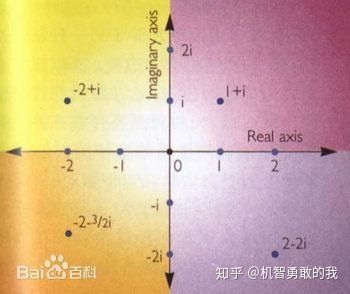
\includegraphics[width=0.7\textwidth]{docs/math/images/fft1.jpg} 
\caption{img}
\end{figure}

其中横坐标是实数轴,纵坐标是虚数轴,这样就可以把每个虚数看为一个向量了,对应的,虚数可以用普通坐标和极坐标 $(r,\theta)$

(其中 $r$ 为虚数长度,$\theta$ 为虚数和实数轴正半轴夹角) 来表示。

接下来思考两个复数相乘是什么意义:

\begin{enumerate}
\item $(a+bi) \times (c+di) = (ac-bd) + (ad+bc)i$
\item 长度相乘,角度相加: $(r_1, \theta_1)  \times  (r_2, \theta_2) = (r_1 \times r_2, \theta_1+\theta_2)$
\end{enumerate}

这么一看的话,我们很容易想到如果两个长度为 $1$ 的不同方向向量相乘,结果向量是不是一个长度依然为 $1$ 的新向量呢?

\subsubsection{单位复根的引入}

我们回到之前的问题:多项式(点值表示法)的乘积。

考虑这样一个问题:

刚刚说到了 DFT 是把多项式从系数表示转到了点值表示(复杂度为 $O(n)$),那么我们把点值相乘之后(选取相应位置,并且复杂度为 $O(n)$),如果能够快速还原成系数表示,是不是就完美解决我们的问题了呢?上述过程如下:

假设我们 DFT 过程对于两个多项式选取的 $x$ 序列相同,那么可以得到

$$
f(x)={(x_0, f(x_0), (x_1, f(x_1)), (x_2, f(x_2), \cdots, (x_n, f(x_n)))}
$$

$$
g(x)={(x_0, g(x_0), (x_1, g(x_1)), (x_2, g(x_2), \cdots, (x_n, g(x_n)))}
$$

如果我们设 $F(x) = f(x) \times g(x0$

那么很容易得到 $F(x)$ 的点值表达式:

$$
F(x) = {(x_0, f(x_0)  \times  g(x_0), (x_1, f(x_1)  \times  g(x_1)), (x_2, f(x_2)  \times  g(x_2), \cdots, (x_n, f(x_n)  \times  g(x_n)))}
$$

但是我们要的是系数表达式,接下来问题变成了从点值回到系数。如果我们带入到高斯消元法的方程组中去,会把复杂度变得非常高。光是计算 $x^i(0 \leq i \leq n)$ 就是 $n$ 项, 这就已经 $O(n^2)$ 了,更别说还要把 $n+1$ 个方程进行消元。。。。。。。。。

这里会不会觉得我们不去计算 $x^i$ 比较好呢?$1$ 和 $-1$ 的幂都很好算,但是也仅仅有两个不够啊,我们至少需要 $n+1$ 个 o(╥﹏╥)o 那怎么办呢!想到我们刚刚学的长度为 $1$ 的虚数了吗?不管怎么乘长度都是 $1$!对就是它!我们需要的是 $\omega^k=1$ 中的 $\omega$,很容易想到 $-i$ 和 $1$ 是符合的。那其他的呢?

\begin{figure}[htbp]
\centering
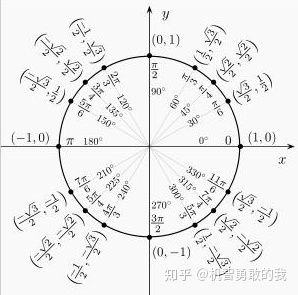
\includegraphics[width=0.7\textwidth]{docs/math/images/fft2.jpg} 
\caption{img}
\end{figure}

现在我们看上图的圆圈。容易发现这是一个单位圆(圆心为原点,半径为 $1$),所有在圆上的复数的长度均为 $1$,也就是说它不管做多少次方 $r$ 永远为 $1$,结果也仅仅角度的变化而已。但是!!!进过旋转总会让角度 $\bmod 360 = 0$ 成立的,也就是结果为 $1$。 我们把符合以上条件的复数成为复根,用 $\omega$ 表示。如果 $\omega^k=1$ 那么我们把$\omega$ 称为 $1$ 的 $k$ 次复根,记作 $\omega_k^n$ (因为符合这个 $k$ 次之后等于 $1$ 的复数有很多,比如 $i$ 的 $4k$ 次幂永远为 $1$,所以,这个 $n$ 是一个编号,表示这是角度从小到大的第几个(从 $x$ 的正半轴开始逆时针))

是不是有点雾啊 ( ̄▽ ̄)/没事没事接下来我们举个栗子:

\begin{figure}[htbp]
\centering
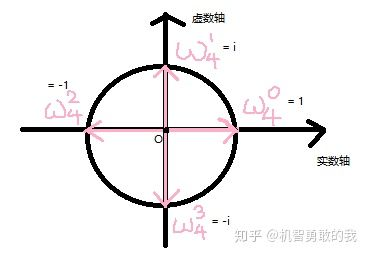
\includegraphics[width=0.7\textwidth]{docs/math/images/fft3.jpg} 
\caption{img}
\end{figure}

那么很容易发现当 $K = 4$ 的时候,相当于把单位圆等分 $K= 4$ 份。然后每一份按照极角编号。那么是不是(在 $K = 4$ 的时候)我们只要知道 $\omega_4^1$

(因为他的角度是相当于单位角度), 就能知道 $\omega_4^0, \omega_4^1, \omega_4^2, \omega_4^3$ 了呢?当然是这样的。。。

$\omega_4^0$ 恒等于 $1$,$\omega_4^2$ 的角度是 $\omega_4^0$ 的两倍,所以 $\omega_4^2 = (\omega_4^1)^2 = i^2=-1$, 依次以此类推。

因此,我们只要知道 $\omega_k^1$ ,就能求出 $\omega_k^n$。所以我们把 $\omega_k^1$ 称为单位复根,简写为 $\omega_k$

\subsection{FFT 的流程}

qwq 终于写到核心部分了,也就是,FFT 到底怎么来写呢?

\subsubsection{FFT 流程第一步之 DFT(共两步)}

FFT 之所以快,是因为他采用了分治的思想。

就 DFT(将系数表达转换成点值表达)来说,它分治的来求当当前的 $x=\omega_n^k$

的时候整个式子的值。他的分治思想体现在将多项式分为奇次项和偶次项处理。

对于一共 $8$ 项的多项式

$$
f(x0) = y_1 = a_0 + a_1x + a_2x^2+a_3x^3+a_4x^4+a_5x^5+a_6x^6+a_7x^7
$$

按照次数的奇偶来分成两组, 然后右边提出来一个 $x$

$$
f(x) = (a_0+a_2x^2+a_4x^4+a_6x^6) + (a_1x+a_3x^3+a_5x^5+a_7x^7)
$$

$$
f(x) = (a_0+a_2x^2+a_4x^4+a_6x^6) + x(a_1+a_3x^2+a_5x^4+a_7x^6)
$$

分别用奇偶次次项数建立新的方程

$$
G(x) = a_0+a_2x+a_4x^2+a_6x^3
$$

$$
H(x)=a_1+a_3x+a_5x^2+a_7x^3
$$

那么原来的 $f(x)$ 由新函数来表示 (是不是我们二分了一个多项式呢\textasciitilde{})

$$
F(x)=G(x^2) + x  \times  H(x^2)
$$

给函数带个帽子表示此时在进行的是 DFT 过程,把 x 代进去,即有

$$
DFT(f(\omega_n^k))=DFT(G((\omega_n^k)^2)) + \omega_n^k  \times  DFT(H((\omega_n^k)^2))
$$

!!!前方高能:

这个函数能处理的多项式长度只能是 $2^m(m \in N^ \times )$ , 否则在分治的时候左右不一样长,右边取不到系数了,程序没法进行。所以要在第一次 DFT 之前就把序列向上补成长度为 $2^m(m \in N^ \times )$(高次系数补 $0$)、最高项次数为 $n-1$ 的多项式。一定要预处理哦 qaq

然后我在代入值的时候,因为要代入 $n$ 个不同值,所以我们就代入 $\omega_n^0,\omega_n^1,\omega_n^2,\cdots, \omega_n^{n-1} (n=2^m(m \in N^ \times ))$

一共 $2^m$ 个不同值。

\begin{cppcode}
/*
 * 做 FFT
 *len 必须是 2^k 形式
 *on == 1 时是 DFT,on == -1 时是 IDFT
 */
void fft(Complex y[], int len, int on) {
  change(y, len);
  for (int h = 2; h <= len; h <<= 1) {
    Complex wn(cos(2 * PI / h), sin(on * 2 * PI / h));
    for (int j = 0; j < len; j += h) {
      Complex w(1, 0);
      for (int k = j; k < j + h / 2; k++) {
        Complex u = y[k];
        Complex t = w * y[k + h / 2];
        y[k] = u + t;
        y[k + h / 2] = u - t;
        w = w * wn;
      }
    }
  }
}
\end{cppcode}

但是这个算法还需要从 “分治” 的角度继续优化。我们每一次都会把整个多项式的奇数次项和偶数次项系数分开,一只分到只剩下一个系数。但是,这个递归的过程需要更多的内存。因此,我们可以先 “模仿递归” 把这些系数在原数组中 “拆分”,然后再 “倍增” 地去合并这些算出来的值。然而我们又要如何去拆分这些数呢?

设初始序列为 $\{x_0, x_1, x_2, x_3, x_4, x_5, x_6, x_7\}$

一次二分之后 $\{x_0, x_2, x_4, x_6\},\{x_1, x_3,x_5, x_7 \}$

两次二分之后 $\{x_0,x_4\} \{x_2, x_6\},\{x_1, x_3\},\{x_5, x_7 \}$

三次二分之后 $\{x_0\}\{x_4\}\{x_2\}\{x_6\}\{x_1\}\{x_3\}\{x_5\}\{x_7 \}$

有啥规律呢?其实就是原来的那个序列,每个数用二进制表示,然后把二进制翻转对称一下,就是最终那个位置的下标。比如 $x_1$ 是 001,翻转是 100,也就是 4,而且最后那个位置确实是 4,是不是很神奇啊\textbackslash{}\textasciitilde{}\textbackslash{}\textasciitilde{}\textasciitilde{}

这里附上代码

\begin{cppcode}
/*
 * 进行 FFT 和 IFFT 前的反置变换
 * 位置 i 和 i 的二进制反转后的位置互换
 *len 必须为 2 的幂
 */
void change(Complex y[], int len) {
  int i, j, k;
  for (int i = 1, j = len / 2; i < len - 1; i++) {
    if (i < j) swap(y[i], y[j]);
    // 交换互为小标反转的元素,i<j 保证交换一次
    // i 做正常的 + 1,j 做反转类型的 + 1,始终保持 i 和 j 是反转的
    k = len / 2;
    while (j >= k) {
      j = j - k;
      k = k / 2;
    }
    if (j < k) j += k;
  }
}
\end{cppcode}

\subsubsection{FFT 流程第二步之 IDFT(共两步)}

这一步 IDFT(傅里叶反变换)的作用我说的已经很清楚啦,就是把上一步获得的目标多项式的点值形式转换成系数形式。但是似乎并不简单呢(雾)。。。但是,我们把单位复根代入多项式之后,就是下面这个样子(矩阵表示方程组)

$$
 \begin{bmatrix}y[0] \\ y[1] \\ y[2] \\ y[3] \\ \dots \\ y[n-1] \end{bmatrix}
\begin{matrix}= \\ = \\ = \\ = \\ \\ = \end{matrix}
\begin{bmatrix}1 & 1 & 1 & 1 & \dots & 1 \\
1 & \omega_n^1 & \omega_n^2 & \omega_n^3 & \dots & \omega_n^{n-1} \\
1 & \omega_n^2 & \omega_n^4 & \omega_n^6 & \dots & \omega_n^{2(n-1)} \\
1 & \omega_n^3 & \omega_n^6 & \omega_n^9 & \dots & \omega_n^{3(n-1)} \\
\dots & \dots & \dots & \dots & \dots & \dots \\
1 & \omega_n^{n-1} & \omega_n^{2(n-1)} & \omega_n^{3(n-1)} & \dots & \omega_n^{(n-1)^2} \end{bmatrix}
\begin{bmatrix} a[0] \\ a[1] \\ a[2] \\ a[3] \\ \dots \\ a[n-1] \end{bmatrix} 
$$

而且现在我们已经得到最左边的结果了,中间的 $x$ 值在目标多项式的点值表示中也是一一对应的,所以,根据矩阵的基础知识,我们只要在式子两边左乘中间那个大矩阵的逆矩阵就行了。由于这个矩阵的元素非常特殊,他的逆矩阵也有特殊的性质,就是每一项取倒数,再除以 $n$,就能得到他的逆矩阵(这边根据的是单位原根的两个特殊性质推出来的,具体比较麻烦。如果想知道的话私我吧。)

如何改变我们的操作才能使计算的结果文原来的倒数呢?我们当然可以重新写一遍,但是这里有更简单的实现。这就要看我们求 “单位复根的过程了”:根据 “欧拉函数” $e^{i\pi}=-1$,我么可以得到 $e^{2\pi i}=1$。如果我要找到一个数,它的 $k$ 次方 $= 1$,那么这个数 $\omega[k]=e^{2\pi \frac{i}{k}}$(因为 $(e^{2\pi \frac{i}{k}})^k=e^{2\pi i}=1$)。而如果我要使这个数值变成$\frac{1}{\omega[k]}$ 也就是 $(\omega[k])^-1$,我们可以尝试着把

$π$ 取成 - 3.14159…,这样我们的计算结果就会变成原来的倒数,而其它的操作过程与 DFT 是完全相同的(这真是极好的)。我们可以定义一个函数,向里面掺一个参数 $1$ 或者是 $-1$,然后把它乘到 $π$ 的身上。传入 $1$ 就是 DFT,传入 $-1$ 就是 IDFT,十分的智能。

所以我们 fft 函数可以集 DFT 和 IDFT 于一身。见下

\begin{cppcode}
/*
 * 做 FFT
 *len 必须是 2^k 形式
 *on == 1 时是 DFT,on == -1 时是 IDFT
 */
void fft(Complex y[], int len, int on) {
  change(y, len);
  for (int h = 2; h <= len; h <<= 1) {                  // 模拟合并过程
    Complex wn(cos(2 * PI / h), sin(on * 2 * PI / h));  // 计算当前单位复根
    for (int j = 0; j < len; j += h) {
      Complex w(1, 0);  // 计算当前单位复根
      for (int k = j; k < j + h / 2; k++) {
        Complex u = y[k];
        Complex t = w * y[k + h / 2];
        y[k] = u + t;  // 这就是吧两部分分治的结果加起来
        y[k + h / 2] = u - t;
        // 后半个 “step” 中的ω一定和 “前半个” 中的成相反数
        //“红圈”上的点转一整圈“转回来”,转半圈正好转成相反数
        // 一个数相反数的平方与这个数自身的平方相等
        w = w * wn;
      }
    }
  }
  if (on == -1) {
    for (int i = 0; i < len; i++) {
      y[i].x /= len;
    }
  }
}
\end{cppcode}

好了现在附上全部代码(\href{http://acm.hdu.edu.cn/showproblem.php?pid=1402}{HDU 1402}),序言说过代码来自 kuangbin 的模板\sout{}\textasciitilde{} 来大家和我一起 Orz 一发

\begin{cppcode}
#include <cmath>
#include <cstdio>
#include <cstring>
#include <iostream>

using namespace std;

const double PI = acos(-1.0);
struct Complex {
  double x, y;
  Complex(double _x = 0.0, double _y = 0.0) {
    x = _x;
    y = _y;
  }
  Complex operator-(const Complex &b) const {
    return Complex(x - b.x, y - b.y);
  }
  Complex operator+(const Complex &b) const {
    return Complex(x + b.x, y + b.y);
  }
  Complex operator*(const Complex &b) const {
    return Complex(x * b.x - y * b.y, x * b.y + y * b.x);
  }
};
/*
 * 进行 FFT 和 IFFT 前的反置变换
 * 位置 i 和 i 的二进制反转后的位置互换
 *len 必须为 2 的幂
 */
void change(Complex y[], int len) {
  int i, j, k;
  for (int i = 1, j = len / 2; i < len - 1; i++) {
    if (i < j) swap(y[i], y[j]);
    // 交换互为小标反转的元素,i<j 保证交换一次
    // i 做正常的 + 1,j 做反转类型的 + 1,始终保持 i 和 j 是反转的
    k = len / 2;
    while (j >= k) {
      j = j - k;
      k = k / 2;
    }
    if (j < k) j += k;
  }
}
/*
 * 做 FFT
 *len 必须是 2^k 形式
 *on == 1 时是 DFT,on == -1 时是 IDFT
 */
void fft(Complex y[], int len, int on) {
  change(y, len);
  for (int h = 2; h <= len; h <<= 1) {
    Complex wn(cos(2 * PI / h), sin(on * 2 * PI / h));
    for (int j = 0; j < len; j += h) {
      Complex w(1, 0);
      for (int k = j; k < j + h / 2; k++) {
        Complex u = y[k];
        Complex t = w * y[k + h / 2];
        y[k] = u + t;
        y[k + h / 2] = u - t;
        w = w * wn;
      }
    }
  }
  if (on == -1) {
    for (int i = 0; i < len; i++) {
      y[i].x /= len;
    }
  }
}

const int MAXN = 200020;
Complex x1[MAXN], x2[MAXN];
char str1[MAXN / 2], str2[MAXN / 2];
int sum[MAXN];

int main() {
  while (scanf("%s%s", str1, str2) == 2) {
    int len1 = strlen(str1);
    int len2 = strlen(str2);
    int len = 1;
    while (len < len1 * 2 || len < len2 * 2) len <<= 1;
    for (int i = 0; i < len1; i++) x1[i] = Complex(str1[len1 - 1 - i] - '0', 0);
    for (int i = len1; i < len; i++) x1[i] = Complex(0, 0);
    for (int i = 0; i < len2; i++) x2[i] = Complex(str2[len2 - 1 - i] - '0', 0);
    for (int i = len2; i < len; i++) x2[i] = Complex(0, 0);
    fft(x1, len, 1);
    fft(x2, len, 1);
    for (int i = 0; i < len; i++) x1[i] = x1[i] * x2[i];
    fft(x1, len, -1);
    for (int i = 0; i < len; i++) sum[i] = int(x1[i].x + 0.5);
    for (int i = 0; i < len; i++) {
      sum[i + 1] += sum[i] / 10;
      sum[i] %= 10;
    }
    len = len1 + len2 - 1;
    while (sum[len] == 0 && len > 0) len--;
    for (int i = len; i >= 0; i--) printf("%c", sum[i] + '0');
    printf("\n");
  }
  return 0;
}
\end{cppcode}

至此,FFT 算是告一段落了。

但是,算竞选手可能像我一样有下面的疑问:

假如我要计算的多项式系数是别的具有特殊意义的整数,那么我通篇都在用浮点数运算,首先从时间上就会比整数运算慢,另外我最多只能用 long double 不能用 long long 类型,我能不能应用数论的变化从而避开浮点运算,达到 “更高更快更强 (・ω\&lt;) ” 呢?

\subsection{算竞选手看过来\textasciitilde{} NTT(数论优化的快速傅里叶变换)}

戳~  NTT 

  \section{快速数论变换}
  
(本文转载自 \href{https://zhuanlan.zhihu.com/c_1005817911142838272}{桃酱的算法笔记},原文戳 \href{https://zhuanlan.zhihu.com/p/41867199}{链接},已获得作者授权)

\subsection{简介}

NTT 解决的是多项式乘法带模数的情况,可以说有些受模数的限制,数也比较大,

但是它比较方便呀毕竟没有复数部分 qwq

\subsection{学习 NTT 之前...}

\subsubsection{生成子群}

子群:群 $(S,⊕), (S′,⊕)$, 满足 $S′⊂S$,则 $(S′,⊕)$ 是 $(S,⊕)$ 的子群

拉格朗日定理:$|S′|∣|S |$ 证明需要用到陪集,得到陪集大小等于子群大小,每个陪集要么不想交要么相等,所有陪集的并是集合 $S$,那么显然成立。

生成子群:$a \in S$ ​的生成子群 $\left<a\right> = \{a^{(k)}, k \geq 1 \}$ ​,$a$ 是 $\left< a \right>$ 的生成元

阶:群 $S$ 中 $a$ 的阶是满足 $a^r=e$ 的最小的 $r$, 符号 $\operatorname{ord}(a)$ , 有 $\operatorname{ord}(a)=\left|\left<a\right>\right|$,显然成立。

考虑群 $Z_n^ \times =\{[a], n \in Z_n : \gcd(a, n) = 1\}, |Z_n^ \times | = \phi(n)$

阶就是满足 $a^r \equiv 1 (\bmod n)$ ​的最小的 $r$,  $\operatorname{ord}(a)=r$

\subsubsection{ 原根 }

$g$ 满足 $\operatorname{ord}_n(g)=\left|Z_n^\times\right|=\phi(n)$,对于质数 $p$,也就是说 $g^i \bmod p, 0 \leq i < p$ 结果互不相同.

模 $n$ 有原根的充要条件 : $n = 2, 4, p^e, 2 \times p^e$

离散对数:$g^t \equiv a (\bmod n),ind_{n,g}{(a)}=t$

​因为 $g$ 是原根,所以 $gt$ 每 $\phi(n)$ 是一个周期,可以取到 $| Z \times n |$ 的所有元素

对于 $n$ 是质数时,就是得到 $[1,n−1]$ 的所有数,就是 $[0,n−2]$ 到 $[1,n−1]$ 的映射

离散对数满足对数的相关性质,如

求原根可以证明满足 $g^r \equiv 1(\bmod p)$

​的最小的 $r$ 一定是 $p−1$ 的约数

对于质数 $p$,质因子分解 $p−1$,若 $g^{(p-1)/pi} \neq 1 (\bmod p)$

​恒成立,$g$ 为 $p$ 的原根

\subsection{NTT}

对于质数 $p=qn+1, (n=2^m)$ ​, 原根 $g$ 满足 $g^{qn} \equiv 1 (\bmod p)$​, 将 $g_n=g^p(\bmod q)$ 看做 $\omega_n$ 的等价,择其满足相似的性质,比如 $g_n^n \equiv 1 (\bmod p), g_n^{n/2} \equiv -1 (\bmod p)$

然后因为这里涉及到数论变化,所以这里的 $N$(为了区分 FFT 中的 n,我们把这里的 n 称为 $N$)可以比 FFT 中的 n 大,但是只要把 $\frac{qN}{n}$ 看做这里的 $q$ 就行了,能够避免大小问题。。。

常见的有

$$
p = 1004535809 = 479 \times 2^{21}, g=3
$$

$$
p=998244353=2 \times 17 \times 2^{23}+1, g=3
$$

就是 $g^{qn}$ 的等价 $e^{2\pi n}$

迭代到长度 $l$ 时 $g_l = g^{\frac{p-1}{l}}$, 或者 $\omega_n = g_l = g_N^{\frac{N}{l}} = g_N^{\frac{p-1}{l}}$

接下来放一个大数相乘的模板

参考网址如下 \url{https://blog.csdn.net/blackjack_/article/details/79346433}

\begin{cppcode}
#include <algorithm>
#include <bitset>
#include <cmath>
#include <cstdio>
#include <cstdlib>
#include <cstring>
#include <ctime>
#include <iomanip>
#include <iostream>
#include <map>
#include <queue>
#include <set>
#include <string>
#include <vector>
using namespace std;

inline int read() {
  int x = 0, f = 1;
  char ch = getchar();
  while (ch < '0' || ch > '9') {
    if (ch == '-') f = -1;
    ch = getchar();
  }
  while (ch <= '9' && ch >= '0') {
    x = 10 * x + ch - '0';
    ch = getchar();
  }
  return x * f;
}
void print(int x) {
  if (x < 0) putchar('-'), x = -x;
  if (x >= 10) print(x / 10);
  putchar(x % 10 + '0');
}

const int N = 300100, P = 998244353;

inline int qpow(int x, int y) {
  int res(1);
  while (y) {
    if (y & 1) res = 1ll * res * x % P;
    x = 1ll * x * x % P;
    y >>= 1;
  }
  return res;
}

int r[N];

void ntt(int *x, int lim, int opt) {
  register int i, j, k, m, gn, g, tmp;
  for (i = 0; i < lim; ++i)
    if (r[i] < i) swap(x[i], x[r[i]]);
  for (m = 2; m <= lim; m <<= 1) {
    k = m >> 1;
    gn = qpow(3, (P - 1) / m);
    for (i = 0; i < lim; i += m) {
      g = 1;
      for (j = 0; j < k; ++j, g = 1ll * g * gn % P) {
        tmp = 1ll * x[i + j + k] * g % P;
        x[i + j + k] = (x[i + j] - tmp + P) % P;
        x[i + j] = (x[i + j] + tmp) % P;
      }
    }
  }
  if (opt == -1) {
    reverse(x + 1, x + lim);
    register int inv = qpow(lim, P - 2);
    for (i = 0; i < lim; ++i) x[i] = 1ll * x[i] * inv % P;
  }
}

int A[N], B[N], C[N];

char a[N], b[N];

int main() {
  register int i, lim(1), n;
  scanf("%s", &a);
  n = strlen(a);
  for (i = 0; i < n; ++i) A[i] = a[n - i - 1] - '0';
  while (lim < (n << 1)) lim <<= 1;
  scanf("%s", &b);
  n = strlen(b);
  for (i = 0; i < n; ++i) B[i] = b[n - i - 1] - '0';
  while (lim < (n << 1)) lim <<= 1;
  for (i = 0; i < lim; ++i) r[i] = (i & 1) * (lim >> 1) + (r[i >> 1] >> 1);
  ntt(A, lim, 1);
  ntt(B, lim, 1);
  for (i = 0; i < lim; ++i) C[i] = 1ll * A[i] * B[i] % P;
  ntt(C, lim, -1);
  int len(0);
  for (i = 0; i < lim; ++i) {
    if (C[i] >= 10) len = i + 1, C[i + 1] += C[i] / 10, C[i] %= 10;
    if (C[i]) len = max(len, i);
  }
  while (C[len] >= 10) C[len + 1] += C[len] / 10, C[len] %= 10, len++;
  for (i = len; ~i; --i) putchar(C[i] + '0');
  puts("");
  return 0;
}
\end{cppcode}

  \section{快速沃尔什变换}
  
(本文转载自 \href{https://zhuanlan.zhihu.com/c_1005817911142838272}{桃酱的算法笔记},原文戳 \href{https://zhuanlan.zhihu.com/p/41867199}{链接},已获得作者授权)

\subsection{简介}

\begin{QUOTE}{}{}
沃尔什转换(Walsh Transform)是在频谱分析上作为离散傅立叶变换的替代方案的一种方法。 —— \href{https://zh.wikipedia.org/zh-cn/\%E6%B2%83%E7%88%BE%E4%BB%80%E8%BD%89%E6%8F%9B}{维基百科}
\end{QUOTE}

其实这个变换在信号处理中应用很广泛,fft 是 double 类型的,但是 walsh 把信号在不同震荡频率方波下拆解,因此所有的系数都是绝对值大小相同的整数,这使得不需要作浮点数的乘法运算,提高了运算速度。

所以,FWT 和 FFT 的核心思想应该是相同的。都是对数组的变换。我们设数组 $A$ 经过快速沃尔什变换之后记作 $FWT[A]$.

那么 FWT 核心思想就是:

我们需要一个新序列 $C$,由序列 $A$ 和序列 $B$ 经过某运算规则得到,即 $C = A \cdot B$

我们先正向得到 $FWT[A], FWT[B]$

然后根据 $FWT[C]=FWT[A] \cdot FWT[B]$

在 $O(n)$ 求出 $FWT[C]$

然后逆向想运算得到原序列 $C$。时间复杂度为 $O(nlogn)$

在算法竞赛中,FWT 是用于解决对下标进行位运算卷积问题的方法。

公式: $C[i] = \sum_{i=j \bigoplus k}A[j] * B[k]$

(其中 $\bigoplus$ 是二元位运算中的某一种,$*$ 是普通乘法)

\subsection{FWT 的运算}

\subsubsection{FWT 之与($\And$)运算和或($|$)运算}

与运算和或运算的本质是差不多的,所以这里讲一下或运算,与运算也是可以自己根据公式 yy 出来的。

\subsubsection{或运算 $A_i$}

如果有 $k=i|j$,那么 $i$ 的二进制位为 $1$ 的位置和 $j$ 的二进制位为 $1$ 的位置肯定是 $k$ 的二进制位为 $1$ 的位置的子集。

现在要得到 $FWT[C] = FWT[A] * FWT[B]$,我们就要构造这个 fwt 的规则。

我们按照定义,显然可以构造 $FWT[A] = A' = \sum_{i=i|j}A[j]$,来表示 $j$ 满足二进制中 $1$ 为 $i$ 的子集。

那么显然会有 $C[i] = \sum_{i=j|k}A[j]*B[k] \Rightarrow FWT[C] = FWT[A] * FWT[B]$

那么我们接下来看 $FWT[A]$ 怎么求。

首先肯定不能枚举了,复杂度为 $O(n^2)$。既然不能整体枚举,我们就考虑分治。

我们把整个区间二分,其实二分区间之后,下标写成二进制形式是有规律可循的。

我们令 $A_0$ 表示 $A$ 的前一半,$A_1$ 表示区间的后一半,那么 $A_0$ 就是 A 下标最大值的最高位为 $0$,他的子集就是他本身的子集(因为最高位为 $0$ 了),但是 $A_1$ 的最高位是 $1$,他满足条件的子集不仅仅是他本身,还包最高位为 $0$ 的子集,即

$$
FWT[A] = merge(FWT[A_0], FWT[A_0] + FWT[A_1])
$$

其中 merge 表示像字符串拼接一样把它们拼起来, $+$ 就是普通加法,表示对应二进制位相加。

这样我们就通过二分能在 $O(logn)$ 完成拼接,每次拼接的时候要完成一次运算,也就是说在 $O(nlogn)$ 的时间复杂度得到了 $FWT[A]$。

接下来就是反演了,其实反演是很简单的,既然知道了 $A_0$ 的本身的子集是他自己 ($A_0 = FAT[A_0]$),$A_1$ 的子集是 $FAT[A_0] + FAT[A_1](A_1'= A_0' + A_1'$), 那就很简单的得出反演的递推式了:

$$
UFWT[A'] = merge(UFWT[A_0'], UFWT[A_1'] - UFWT[A_0'])
$$

\subsubsection{与运算}

与运算类比或运算可以得到类似结论

$$
FWT[A] = merge(FWT[A_0] + FWT[A_1], FWT[A_1])
$$

$$
UFWT[A'] = merge(UFWT[A_0'] - UFWT[A_1'], UFWT[A_1'])
$$

\subsubsection{异或运算}

最常考的异或运算。

异或的卷积是基于如下原理:

若我们令 $i\And j$ 中 $1$ 数量的奇偶性为 $i$ 与 $j$ 的奇偶性,那么 $i$ 与 $k$ 的奇偶性异或 $j$ 和 $k$ 的奇偶性等于 $i \operatorname{xor} j$ 和 $k$ 的奇偶性。

对于 $FWT[A]$ 的运算其实也很好得到。

公式如下:

$A[i] = \sum_{C_1}A[j] - \sum_{C_2}A[j]$ ($C_1$ 表示 $i \And j$ 奇偶性为 $0$,$C_2$ 表示 $i \And j$ 的奇偶性为 $1$)

结论:

$$
FWT[A] = merge(FWT[A_0] + FWT[A_1], FWT[A_0] - FWT[A_1])
$$

$$
UFWT[A'] - merge(\frac{FWT[A_0'] + FWT[A_1']}{2}, \frac{FWT[A_0'] - FWT[A_1']}{2})
$$

\subsubsection{同或运算}

类比异或运算给出公式:

$A[i] = \sum_{C_1}A[j] - \sum_{C_2}A[j]$ ($C_1$ 表示 $i|j$ 奇偶性为 $0$,$C_2$ 表示 $i|j$ 的奇偶性为 $1$)

$$
FWT[A] = merge(FWT[A_1] - FWT[A_0], FWT[A_1] + FWT[A_0])
$$

$$
UFWT[A'] = merge(\frac{FWT[A_1'] - FWT[A_0']}{2}, \frac{FWT[A_1'] + FWT[A_0']}{2})
$$

  \section{排列组合}
  
\subsection{排列组合简介}

排列组合是组合数学中的一种。排列就是指从给定个数的元素中取出指定个数的元素进行排序;组合则是指从给定个数的元素中仅仅取出指定个数的元素,不考虑排序。排列组合的中心问题是研究给定要求的排列和组合可能出现的情况总数。 排列组合与古典概率论关系密切。

在高中初等数学中,排列组合多是利用列表、枚举等方法解题。

\hr

\subsection{排列组合公式及定义}

\subsubsection{排列的定义}

从 $n$ 个不同元素中,任取 $m$($m≤n,m$ 与 $n$ 均为自然数, 下同)个元素按照一定的顺序排成一列,叫做从 $n$ 个不同元素中取出 $m$ 个元素的一个排列;从 $n$ 个不同元素中取出 $m$($m≤n$) 个元素的所有排列的个数,叫做从 $n$ 个不同元素中取出 $m$ 个元素的排列数,用符号 $A_n^m$ 表示。

\subsubsection{排列的计算公式}

$$
A_n^m = n(n-1)(n-2) \cdots (n-m+1) = \frac{n!}{(n - m)!}
$$

\textbf{$n!$ 代表 $n$ 的阶乘,即 $6! = 1 \times 2 \times 3 \times 4 \times 5 \times 6$.}

\subsubsection{组合的定义}

从 $n$ 个不同元素中,任取 $m$($m≤n$) 个元素并成一组,叫做从 $n$ 个不同元素中取出 $m$ 个元素的一个组合;从 $n$ 个不同元素中取出 $m$($m≤n$) 个元素的所有组合的个数,叫做从 $n$ 个不同元素中取出 $m$ 个元素的组合数。用符号 $C_n^m$ 表示。

\subsubsection{组合的计算公式}

$$
C_n^m = \frac{A_n^m}{m!} = \frac{n!}{m!(n - m)!}
$$

\subsection{排列组合的分类}

\subsubsection{排列}

\textbf{ 全排列 }:  

$n$ 个人全部来排队,队长为 $n$。第一个位置可以选 $n$ 个,第二位置可以选 $n-1$ 个,以此类推得:

$$
A_n^n = n(n-1)(n-2) \cdots 3 × 2 × 1 = n!
$$

\textbf{ 部分排列 }:  

$n$ 个人选 $m$ 个来排队 ($m \le n$)。第一个位置可以选 $n$ 个,第二位置可以选 $n-1$ 个,以此类推,第 $m$ 个(最后一个)可以选 $n-m+1$ 个,得:

$$
A_n^m = n(n-1)(n-2) \cdots (n-m+1) = \frac{n!}{(n - m)!}
$$

\subsubsection{组合}

$n$ 个人 $m$($m \le n$) 个出来,不排队,不在乎顺序 $C_n^m$。如果在乎排列那么就是 $A_n^m$,如果不在乎那么就要除掉重复,那么重复了多少?同样选出的来的 $m$ 个人,他们还要 “全排” 得 $A_n^m$,所以得:

$$
C_n^m \times m! = A_n^m
$$

$$
C_n^m = \frac{A_n^m}{m!} = \frac{n!}{m!(n-m)!}
$$

\paragraph{组合数的性质}

$$
C_n^m = C_{n}^{n-m}
$$

$$
C_n^m = C_{n-1}^{m} + C_{n-1}^{m-1}
$$

如果编程实现,以上两个公式有没有帮助?

\subsubsection{圆排列}

$n$ 个人全部来围成一圈为 $Q_n^n$,其中已经排好的一圈,从不同位置断开,又变成不同的队列。  

所以:

$$
Q_n^n \times n = A_n^n → Q_n = \frac{A_n^n}{n} = (n-1)!
$$

\textbf{ 由此可知:部分圆排 }

$$
Q_n^r = \frac{A_n^r}{r} = \frac{n!}{r \times (n-r)!}
$$

\subsubsection{重复排列(有限)}

$k$ 种不一样的球,每种球的个数分别是 $a_1,a_2,\cdots,a_k$,设 $n=a_1+a_2+…+a_k$,这 $n$ 个球的全排列数,为

$$
\frac{n!}{a_1! \times a_2! \times \cdots \times a_k!}
$$

\subsubsection{重复组合(无限)}

$n$ 种不一样的球,每种球的个数是无限的, 从中选 $k$ 个出来,不用排列,是组合,为 $C_{n+k-1}^{k}$.

证明:

\begin{QUOTE}{}{}
假设选出来的数(排好序):
\end{QUOTE}

$$
1 \le b_1 \le b_2 \le b_3 \le \cdots \le b_k \le n
$$

\begin{QUOTE}{}{}
这题的难点就是 $=$ 号,现在去掉 $=$ 号,所以有:
\end{QUOTE}

$$
1 \le b_1 < b_2+1 < b_3+2 < b_4+3 < \cdots < b_k+k-1 \le n+k-1
$$

中间还是 $k$ 个数!不过已经不是 $b$ 系列,而是 $c$ 系列,\textbf{ 假设 $c[i]=b[i]+i-1$,所以 }

$$
1 \le c_1 < c_2 < c_3 < c_4 < \cdots < c_k \le n+k-1
$$

所以问题就开始转换为无重复组合问题,即在 $n+k-1$ 个元素中选中 $k$ 个的组合数 $C_{n+k-1}^{k}$。

\subsubsection{不相邻的排列}

$1 \sim n$ 这 $n$ 个自然数中选 $k$ 个,这 $k$ 个数中任何两个数不相邻数的组合有 $C_{n-k+1}^{k}$ 种。  

证明和上面的相同(其实就是懒得写),请自行证明 XD

\subsubsection{错位排列(错排)}

先看一个小问题:  

$5$ 本书,编号分别是 $1,2,3,4,5$,现在要把这 5 本书是放在编号 $1,2,3,4,5$ 的书架上,要求书的编号和书架的编号不一样,请问有多少种不一样的放置方法?

再看一个小问题:  

胸口贴着编号为 $1,2,\cdots,n$ 的 $n$ 个球员分别住在编号为 $1,2,\cdots,n$ 的 $n$ 个房间里面。现规定每个人住一个房间,自己的编号不能和房间的编号一样。

这就是错排问题。当 $n=3$ 时,只能为 312 或 231 这两种。

那么错排问题的解题思路是什么呢?我们以第二个问题为例:

\textbf{ 递推还是王道!!!}

刚开始所有球员都住在和自己编号一样的房间里面。然后错排开始了,第 $n$ 个球员从第 $n$ 个房间出来。

第一种情况:  

$n$ 想和 $i(1 \le i \le n-1)$ 其中任何一个球员换房间,其他 $n-2$ 个人换房间的事情,他们就不管了。其他 $n-2$ 个球员的的错排数为 $d[n-2]$,$n$ 可以和前面 $1 \sim n-1$ 对换,所以有 $n-1$ 个 $d[n-2]$。

第二种情况:  

$n$ 想和 $i(1 \le i \le n-1)$ 其中任何一个球员换房间,但是 $n$ 只想 $i$ 住在第 $N$ 个房间,而 $n$ 不想住第 $I$ 个房间。

可能你会这样想:那么 $n$ 可以让 $j$ 住在第 $I$ 号房间里面,然后 $n$ 住在房间 $J$。抱歉,$j(1 \le j \le n-1,j\neq i)$ 生气 $n$ 为什么一开始就去找 $i$ 不直接来找 $j$。没办法,$n$ 把自己胸口的编码 $N$ 换成了 $I$,他假装自己是 $i$,然后错排 $1 \sim n-1$(也就是 $d[n-2]$)的时候参与进去,这样自己就不会呆在第 $I$ 号房间了。所以有 $n-1$ 个 $d[n-1]$。

如果理解了以上内容,那么错排的公式就出来了:

$$
d_n = (n-1)(d_{n-2} + d_{n-1}) (n\geq 3)
$$

同时也有:

$$
d_n = n \times d_{n-1} + (-1)^n
$$

错位排列数列为 $0,1,2,9,44,265,\cdots$

\subsection{加法 \& 乘法原理}

\subsubsection{加法原理}

完成一个工程可以有 $n$ 类办法,$a[i](1 \le i \le n)$ 代表第 $i$ 类方法的数目。  

那么完成这件事共有 $S=a[1]+a[2]+\cdots +a[n]$ 种不同的方法。

\subsubsection{乘法原理}

完成一个工程需要分 $n$ 个步骤,$a[i](1 \le i \le n)$ 代表第 $i$ 个步骤的不同方法数目。  

那么完成这件事共有 $S = a[1] \times a[2] \times \cdots \times a[n]$ 种不同的方法。

\subsubsection{两原理的区别}

\textbf{ 一个与分类有关,一个与分步有关;加法原理是 “分类完成”,乘法原理是 “分步完成”。}

\subsection{几个关于组合的公式}

$$
C_n^0 + C_n^1 + C_n^2 + C_n^3 + \cdots + C_n^m = 2^n
$$

$$
C_n^r + C_n^{r+1} = C_{n+1}^{r+1}
$$

$$
\sum_{i=0}^m C_n^i C_m^{m-i} = C_{m+n}^m(n \geq m)
$$

  \section{卡特兰数}
  
\subsection{Catalan 数列}

以下问题属于 Catalan 数列:

\begin{enumerate}
\item 有 $2n$ 个人排成一行进入剧场。入场费 5 元。其中只有$n$个人有一张 5 元钞票,另外 $n$ 人只有 10 元钞票,剧院无其它钞票,问有多少中方法使得只要有 10 元的人买票,售票处就有 5 元的钞票找零?
\item 一位大城市的律师在她住所以北 $n$ 个街区和以东 $n$ 个街区处工作。每天她走 $2n$ 个街区去上班。如果他从不穿越(但可以碰到)从家到办公室的对角线,那么有多少条可能的道路?
\item 在圆上选择 $2n$ 个点, 将这些点成对连接起来使得所得到的 $n$ 条线段不相交的方法数?
\item 对角线不相交的情况下,将一个凸多边形区域分成三角形区域的方法数?
\item 一个栈 (无穷大) 的进栈序列为 $1,2,3, \cdots ,n$ 有多少个不同的出栈序列?
\item $n$ 个结点可够造多少个不同的二叉树?
\item $n$ 个不同的数依次进栈,求不同的出栈结果的种数?
\item $n$ 个 $+1$ 和 $n$ 个 $-1$ 构成 $2n$ 项 $a_1,a_2, \cdots ,a_{2n}$,其部分和满足 $a_1+a_2+ \cdots +a_k>=0(k=1,2,3, \cdots ,2n)$ 对与 $n$ 该数列为?
\end{enumerate}

其对应的序列为:

\begin{tabular}{cccccccc}
\hline
H\_0& H\_1& H\_2& H\_3& H\_4& H\_5& H\_6& ...\\1& 1& 2& 5& 14& 42& 132& ...\\\hline
\end{tabular}

(Catalan 数列)

该递推关系的解为:

$$
H_n=\frac{C_{2n}^{n}}{n+1}(n=1,2,3,\cdots)
$$

  \section{斯特林数}
  
\subsection{Stirling 数(子集划分)}

根据例题来讲解:  

(2007 普及)将$n$个数$(1,2,…,n)$分成$r$个部分。每个部分至少一个数。将不同划分方法的总数记为$S_n^r$。例如,$S_4^2=7$,这 7 种不同的划分方法依次为 $\{\ (1) , (234) \}\,\{\ (2) ,  (134) \}\,\{\ (3) , (124) \}\,\{\ (4) , (123) \}\,\{\ (12) , (34) \}\,\{\ (13) , (24) \}\,\{\ (14) , (23) \}$。当$n=6,r=3$时,$S_6^3$=(    )  

\begin{QUOTE}{}{}
提示:先固定一个数,对于其余的 5 个数考虑$S_5^3$与$S_5^2$,再分这两种情况对原固定的数进行分析。
\end{QUOTE}

题解:在近几年算法竞赛中,递推算法越来越重要:

$$
S_6^3=3 \times S_5^3 + S_5^2
$$

$$
S_5^3=3 \times S_4^3 + S_4^2
$$

$$
S_5^2=2 \times S_4^2 + S_4^1
$$

第二类 stirling 数,显然拥有这样的性质:

$$
S_n^m = m \times S_{n-1}^{m} + S_{n-1}^{m-1}
$$

$$
S_n^1 = 1,S_n^0 = 0,S_n^n = 1
$$

而这些性质就可以总结成:

$$
S_n^3 = \frac{1}{2} \times (3^{n-1}+1) - 2^{n-1}
$$

  \section{康托展开}
  
康托展开可以用来求一个 $1\sim n$ 的任意排列的排名。

\subsection{什么是排列的排名?}

把 $1\sim n$ 的所有排列按字典序排序,这个排列的位次就是它的排名。

\subsection{时间复杂度?}

康托展开可以在 $O(n^2)$ 的复杂度内求出一个排列的排名,在用到树状数组优化时可以做到 $O(n\log n)$ 。

\subsection{怎么实现?}

因为排列是按字典序排名的,因此越靠前的数字优先级越高。也就是说如果两个排列的某一位之前的数字都相同,那么如果这一位如果不相同,就按这一位排序。

比如 $4$ 的排列,$[2,3,1,4]<[2,3,4,1]$,因为在第 $3$ 位出现不同,则 $[2,3,1,4]$ 的排名在 $[2,3,4,1]$ 前面。

\subsection{举个栗子}

我们知道长为 $5$ 的排列 $[2,5,3,4,1]$ 大于以 $1$ 为第一位的任何排列,以 $1$ 为第一位的 $5$ 的排列有 $4!$ 种。这是非常好理解的。但是我们对第二位的 $5$ 而言,它大于\textbf{第一位与这个排列相同的,而这一位比 $5$ 小的}所有排列。不过我们要注意的是,这一位不仅要比 $5$ 小,还要满足没有在当前排列的前面出现过,不然统计就重复了。因此这一位为 $1,3$ 或 $4$ ,第一位为 $2$ 的所有排列都比它要小,数量为 $3\times 3!$。

按照这样统计下去,答案就是 $1+4!+3\times 3!+2!+1=46$。注意我们统计的是排名,因此最前面要 $+1$。

注意到我们每次要用到\textbf{当前有多少个小于它的数还没有出现},这里用树状数组统计比它小的数出现过的次数就可以了。

\subsection{逆康托展开}

因为排列的排名和排列是一一对应的,所以康托展开满足双射关系,是可逆的。可以通过类似上面的过程倒推回来。

如果我们知道一个排列的排名,就可以推出这个排列。因为 $4!$ 是严格大于 $3\times 3!+2\times 2!+1\times 1!$ 的,所以可以认为对于长度为 $5$ 的排列,排名 $x$ 除以 $4!$ 向下取整就是有多少个数小于这个排列的第一位。

\subsection{引用上面展开的例子}

首先让 $46-1=45$,$45$ 代表着有多少个排列比这个排列小。$\lfloor\frac {45}{4!}\rfloor=1$,有一个数小于它,所以第一位是 $2$。

此时让排名减去 $1\times 4!$得到$21$,$\lfloor\frac {21}{3!}\rfloor=3$,有 $3$ 个数小于它,去掉已经存在的 $2$,这一位是 $5$。

$21-3\times 3!=3$,$\lfloor\frac {3}{2!}\rfloor=1$,有一个数小于它,那么这一位就是 $3$。

让 $3-1\times 2!=1$,有一个数小于它,这一位是剩下来的第二位,$4$,剩下一位就是 $1$。即 $[2,5,3,4,1]$。

实际上我们得到了形如\textbf{有两个数小于它}这一结论,就知道它是当前第 $3$ 个没有被选上的数,这里也可以用线段树维护,时间复杂度为 $O(n\log n)$。

  \section{容斥原理}
  
假设班里有 $10$ 个学生喜欢数学, $15$ 个学生喜欢语文, $21$ 个学生喜欢编程,班里至少喜欢一门学科的有多少个学生呢?是 $10+15+21=46$ 个吗?不是的,因为有些学生可能同时喜欢数学和语文,或者语文和编程,甚至还有可能三者都喜欢。为了叙述方便,我们把喜欢语文、数学、编程的学生集合分别用 $A,B,C$ 表示,则学生总数等于 $|A\cup B\cup C|$。刚才已经讲过,如果把这三个集合的元素个数 $|A|,|B|,|C|$ 直接加起来,会有一些元素重复统计了,因此需要扣掉 $|A\cap B|,|B\cap C|,|C\cap A|$ ,但这样一来,又有一小部分多扣了,需要加回来,即 $|A\cap B\cap C|$ 。即

$|A\cup B\cup C|=|A|+|B|+|C|-|A\cap B|-|B\cap C|-|C\cap A|+|A\cap B\cap C|$

一般地,对于任意多个集合,我们都可以列出这样一个等式,等式左边是所有集合的并的元素个数,右边是这些集合的各种搭配。每个搭配都是若干个集合的交集,且每一项前面的正负号取决于集合的个数————奇数个集合为正,偶数个集合为负。即

设 $S$ 为有限集, $A_i\in S~(i=1,2,...,n~,~n\ge 2)$ ,则有

$| \bigcup_{i=1}^n A_i | =\sum_{k=1}^n (-1)^{(k-1)} \times \sum_{1\le i_1<i_2<...<i_k\le n} |A_{i_1}\cap A_{i_2} \cap ...\cap A_{i_k}|$

\subsection{容斥原理在算法竞赛中的应用}

\begin{NOTE}{例题 \href{https://www.lydsy.com/JudgeOnline/problem.php?id=1042}{BZOJ 1042 HAOI2008 硬币购物}}{}
题目大意:一共有 $4$ 种硬币,面值分别为 $c_1,c_2,c_3,c_4$ 。某人去买东西,去了 $tot$ 次。每次给出 $d1,d2,d3,d4$ ,$d_i$ 表示有 $i$ 个面值为 $c_i$ 的硬币,求购买价值为 $s$ 的物品的付款方案数。

\end{NOTE}


先用完全背包预处理出 $f(i)$ ,表示不限制钞票数量购买价格为 $i$ 的物品的方案数。由于容斥原理,我们最后的答案为

$f(s)-f(s-d_1)-f(s-d_2)-f(s-d_3)-f(s-d_4)$

$+f(s-d_1-d_2)+f(s-d_1-d_3)+f(s-d_1-d_4)+f(s-d_2-d_3)+f(s-d_2-d_4)+f(s-d_3-d_4)$

$-f(s-d_1-d_2-d_3)-f(s-d_1-d_2-d_4)-f(s-d_1-d_3-d_4)-f(s-d_2-d_3-d_4)+f(s-d_1-d_2-d_3-d_4)$

这样,我们就可以在 $O(1)$ 的时间复杂度内处理每个询问。

\subsubsection{练习}

\href{https://www.lydsy.com/JudgeOnline/problem.php?id=4665}{BZOJ 4665 小 w 的喜糖}

\href{https://www.lydsy.com/JudgeOnline/problem.php?id=4361}{BZOJ 4361 isn}

  \section{抽屉原理}
  
就比如说,你有 $n+1$ 个苹果,想要放到 $n$ 个抽屉里,那么必然会有至少一个抽屉里有两个(或以上)的苹果。

这个定理看起来比较显然,证明方法考虑反证法:假如所有抽屉都至多放了一个苹果,那么 $n$ 个抽屉至多只能放 $n$ 个苹果,矛盾。

\section{概率 \& 期望}

\subsection{事件}

\subsubsection{单位事件、事件空间、随机事件}

在一次随机试验中可能发生的不能再细分的结果被称为单位事件,用 $E$ 表示。在随机试验中可能发生的所有单位事件的集合称为事件空间,用 $S$ 来表示。例如在一次掷骰子的随机试验中,如果用获得的点数来表示单位事件,那么一共可能出现 $6$ 个单位事件,则事件空间可以表示为 $S=\{1,2,3,4,5,6\}$ 。

随机事件是事件空间 $S$ 的子集,它由事件空间 $S$ 中的单位元素构成,用大写字母 $A, B, C,\ldots$ 表示。例如在掷两个骰子的随机试验中,设随机事件 $A$ 为 “获得的点数和大于 $10$ ” ,则 $A$ 可以由下面 $3$ 个单位事件组成: $A = \{ (5,6),(6,5),(6,6)\}$ 。

\subsubsection{事件的计算}

因为事件在一定程度上是以集合的含义定义的,因此可以把集合计算方法直接应用于事件的计算,也就是说,在计算过程中,可以把事件当作集合来对待。

\textbf{ 和事件 } :相当于 \textbf{ 并集 } 。只需其中之一发生,就发生了。

\textbf{ 积事件 } :相当于 \textbf{ 交集 } 。必须要全都发生,才计算概率。

\subsection{概率}

\subsubsection{定义}

如果在相同条件下,进行了 n 次试验,事件 A 发生了$N_A$ 次,那么$\frac{N_A}{n}$ 称为事件 A 发生的概率。

\subsubsection{公理}

\textbf{ 非负性 } :对于一个事件 $A$ ,有概率 $P(A)\in [0,1]$ 。

\textbf{ 规范性 } :事件空间的概率值为 $1$,$P(S)=1$.

\textbf{ 容斥性 } :若 $P(A+B) = P(A)+P(B)$ ,则  $A$ 和 $B$ 互为独立事件。

\subsubsection{计算}

\textbf{ 全概率公式 } :若事件 $A_1,A_2,\ldots,A_n$ 构成一个完备的事件且都有正概率,即 $\forall i,j, A_i\cap A_j=\varnothing$ 且 $\displaystyle \sum_{i=1}^n A_i=1$,有 $\displaystyle P(B)=\sum_{i=1}^n P(A_i)P(B|A_i)$ 。

\textbf{ 贝叶斯定理 } : $\displaystyle P(B_i|A)=\frac{P(B_i)P(A|B_i)}{\displaystyle \sum_{j=1}^n P(B_j)P(A|B_j)}$

公式中,事件 $B_i$ 的概率为 $P(B_i)$ ,事件 $B_i$ 已发生条件下事件 $A$ 的概率为 $P(A|B_i)$ ,事件 $A$ 发生条件下事件 $B_i$ 的概率为 $P(B_i|A)$ 。

\subsection{期望}

\subsubsection{定义}

在一定区间内变量取值为有限个,或数值可以一一列举出来的变量称为离散型随机变量。一个离散性随机变量的数学期望是试验中每次可能的结果乘以其结果概率的总和。

\subsubsection{性质}

\textbf{ 全期望公式 } : $E(Y)=E[E(Y|X)]$ 。可由全概率公式证明。

\textbf{ 线性性质 } : 对于任意两个随机事件 $x,y$ ( \textbf{ 不要求相互独立 } ) ,有 $E(X+Y)=E(X)+E(Y)$ 。

\subsection{例题}

\href{https://ti.luogu.com.cn/problemset/1022}{NOIP2017 初赛 T14, T15}

\href{https://www.luogu.org/problemnew/show/P1850}{NOIP2016 换教室} (概率期望 DP)

\section{置换群}



\section{数值积分}



\section{线性规划}



\section{博弈论}

\textbf{ 博弈论 },是经济学的一个分支,主要研究具有竞争或对抗性质的对象,在一定规则下产生的各种行为。博弈论考虑游戏中的个体的预测行为和实际行为,并研究它们的优化策略。

通俗地讲,博弈论主要研究的是:在一个游戏中,进行游戏的多位玩家的策略。

\subsection{公平组合游戏}

公平组合游戏的定义如下:

\begin{itemize}
\item 游戏有两个人参与,二者轮流做出决策。且这两个人的决策都对自己最有利。
\item 游戏中的同一个状态不可能多次抵达。且游戏不会有平局出现。
\item 任意一个游戏者在某一确定状态可以作出的决策集合只与当前的状态有关,而与游戏者无关。
\end{itemize}

大部分的棋类游戏都是公平组合游戏,如国际象棋、中国象棋、围棋、五子棋等。

\subsection{Nim 游戏}

$n$ 堆物品,每堆有 $a_i$ 个,两个玩家轮流取走任意一堆的任意个物品,但不能不取。

取走最后一个物品的人获胜。

例如,如果现在有 $n=3$ 堆物品,而每堆分别有 $2, 5, 4$ 个,那么可以取走第 $1$ 堆中的 $2$ 个物品,局面就变成了 $0, 5, 4$ ;或者也可以取走第 $2$ 堆的 $4$ 个物品,局面就变成了 $2, 1, 4$ 。

如果现在的局面为 $0, 0, 5$ ,甲取走了第 $3$ 堆的 $5$ 个物品,也就是取走了最后一个物品,此时甲获胜。

\subsection{博弈图和状态}

如果将每个状态视为一个节点,再从每个状态向它的后继状态连边,我们就可以得到一个博弈状态图。

例如,如果节点 $(i, j, k)$ 表示局面为 $i, j, k$ 时的状态,则我们可以画出下面的博弈图(由于篇幅有限,故仅显示部分状态节点和部分边):

\begin{figure}[htbp]
\centering
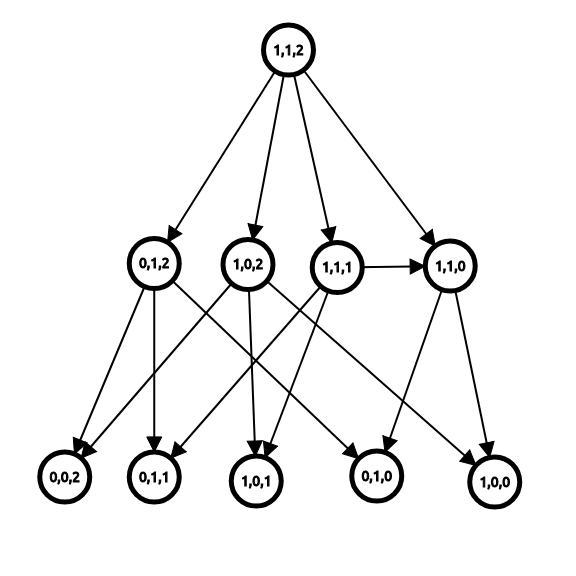
\includegraphics[width=0.7\textwidth]{docs/math/images/game1.png} 
\caption{博弈图的例子}
\end{figure}

定义 \textbf{ 必胜状态 } 为 \textbf{ 先手必胜的状态 },\textbf{ 必败状态 } 为 \textbf{ 先手必败的状态 }。

通过推理,我们可以得出下面三条定理:

\begin{itemize}
\item 定理 1:没有后继状态的状态是必败状态。
\item 定理 2:一个状态是必胜状态当且仅当存在至少一个必败状态为它的后继状态。
\item 定理 3:一个状态是必败状态当且仅当它的所有后继状态均为必胜状态。
\end{itemize}

对于定理 1,如果游戏进行不下去了,那么这个玩家就输掉了游戏。

对于定理 2,如果该状态至少有一个后继状态为必败状态,那么玩家可以通过操作到该必败状态;此时对手的状态为必败状态——对手必定是失败的,而相反地,自己就获得了胜利。

对于定理 3,如果不存在一个后继状态为必败状态,那么无论如何,玩家只能操作到必胜状态;此时对手的状态为必胜状态——对手必定是胜利的,自己就输掉了游戏。

如果博弈图是一个有向无环图,则通过这三个定理,我们可以在绘出博弈图的情况下用 $O(N+M)$ 的时间(其中 $N$ 为状态种数, $M$ 为边数)得出每个状态是必胜状态还是必败状态。

\subsection{Nim 和}

让我们再次回顾 Nim 游戏。

通过绘画博弈图,我们可以在 $O(a_1 \cdot a_2 \cdot \ldots \cdot a_n)$ 的时间里求出该局面是否先手必赢。

但是,这样的时间复杂度实在太高。有没有什么巧妙而快速的方法呢?

定义 Nim 和 $=a_1 \oplus a_2 \oplus \ldots \oplus a_n$。

当且仅当 Nim 和为 $0$ 时,该状态为必败状态;否则该状态为必胜状态。

\subsubsection{证明}

为什么异或值会和状态的胜负有关?下面给出了这个定理的证明过程。

为了证明该定理,只需要证明下面三个定理:

\begin{itemize}
\item 定理 1:没有后继状态的状态是必败状态。
\item 定理 2:对于 $a_1 \oplus a_2 \oplus \ldots \oplus a_n \neq 0$ 的局面,一定存在某种移动使得 $a_1 \oplus a_2 \oplus \ldots \oplus a_n = 0$ 。
\item 定理 3:对于 $a_1 \oplus a_2 \oplus \ldots \oplus a_n = 0$ 的局面,一定不存在某种移动使得 $a_1 \oplus a_2 \oplus \ldots \oplus a_n = 0$ 。
\end{itemize}

对于定理 1,没有后继状态的状态只有一个,即全 $0$ 局面。此时 $a_1 \oplus a_2 \oplus \ldots \oplus a_n = 0$ 。

对于定理 2,不放假设 $a_1 \oplus a_2 \oplus \ldots a_n = k \neq 0$ 。如果我们要将 $a_i$ 改为 $a_i'$ ,则 $a_i'=a_i \oplus k$ 。

根据异或定义,一定有奇数个 $a_i$ 在 $k$ 在二进制下的最高位为 $1$ 。满足这个条件的 $a_i$ 一定也满足 $a_i > a_i \oplus k$ ,因而这也是个合法的移动。

对于定理 3,如果我们要将 $a_i$ 改为 $a_i'$ ,则根据异或运算律可以得出 $a_i=a_i'$ ,因而这不是个合法的移动。

\subsection{有向图游戏与 SG 函数}

有向图游戏是一个经典的博弈游戏——实际上,大部分的公平组合游戏都可以转换为有向图游戏。

在一个有向无环图中,只有一个起点,上面有一个棋子,两个玩家轮流沿着有向边推动棋子,不能走的玩家判负。

定义 $mex$ 函数的值为不属于集合 $S$ 中的最小非负整数,即:

$$
mex(S)=min\{x\} \quad (x \notin S, x \in N)
$$

例如 $mex(\{0, 2, 4\})=1$ , $mex(\{1, 2\})=0$ 。

对于状态 $x$ 和它的所有 $k$ 个后继状态 $y_1, y_2, \ldots, y_k$ ,定义 $SG$ 函数:

$$
SG(x)=mex\{SG(y_1), SG(y_2), \ldots, G(y_k)\}
$$

而对于由 $n$ 个有向图游戏组成的组合游戏,设它们的起点分别为 $s_1, s_2, \ldots, s_n$ ,则有定理:\textbf{ 当且仅当 $SG(s_1) \oplus SG(s_2) \oplus \ldots \oplus SG(s_n) \neq 0$ 时,这个游戏是先手必胜的。}

这一定理被称作 SG 定理。

\subsection{将 Nim 游戏转换为有向图游戏}

我们可以将一个有 $x$ 个物品的堆视为节点 $x$ ,则当且仅当 $y<x$ 时,节点 $x$ 可以到达 $y$ 。

那么,由 $n$ 个堆组成的 Nim 游戏,就可以视为 $n$ 个有向图游戏了。

根据上面的推论,可以得出 $SG(x)=x$ 。再根据 SG 定理,就可以得出 Nim 和的结论了。

\subsection{参考文献}

\href{http://www.cnblogs.com/exponent/articles/2141477.html}{(转载)Nim 游戏博弈 (收集完全版) - exponent - 博客园}

\href{https://www.cnblogs.com/candy99/p/6548836.html}{组合游戏与博弈论【学习笔记】 - Candy? - 博客园}

\section{杂项}
本文主要介绍了在 OI 中可能用到的重要高中数学知识。

如果是高中 OIer,强烈建议回班级听课。

下面按照从必修到选修的顺序介绍。所有内容均基于人教版高中数学 A 版教科书。

\subsection{向量}

(为人教版高中数学 A 版教科书必修四内容)

\begin{QUOTE}{}{}
平面的向量交错生长



织成



忧伤的网



——《膜你抄》
\end{QUOTE}

\subsubsection{定义及相关概念}

\textbf{向量}:既有大小又有方向的量称为向量。

\textbf{有向线段}:带有方向的线段称为有向线段。有向线段有三要素:\textbf{起点,方向,长度},知道了三要素,终点就唯一确定。我们用有向线段表示向量。

\textbf{向量的模}:有向线段 $\vec{AB}$ 的长度称为向量的模,即为这个向量的大小。记为:$|\vec{AB}|$。

\textbf{零向量}:模为 $0$ 的向量。零向量的方向任意。记为: $\vec{0}$ 或 $\mathbf{0}$。

\textbf{单位向量}:模为 $1$ 的向量称为该方向上的单位向量。

\textbf{平行向量}:方向相同或相反的两个\textbf{非零}向量。记作:$\vec a\parallel \vec b$。

\textbf{相等向量}:模相等且方向相同的向量。

\textbf{相反向量}:模相等且方向相反的向量。

\textbf{向量的夹角}:已知两个非零向量 $\vec a,\vec b$,作 $\vec{OA}=\vec a,\vec{OB}=\vec b$,那么 $\theta=\angle \text{AOB}$ 就是向量 $\vec a$ 与向量 $\vec b$ 的夹角。记作:$\langle \vec a,\vec b\rangle$。显然当 $\theta =0$ 时两向量同向,$\theta=\pi$ 时两向量反向,$\theta=\frac{\pi}{2}$ 时我们说两向量垂直,记作 $\vec a\perp \vec b$。并且,我们规定 $\theta \in [0,\pi]$。

(呼…… 我们一口气把数学书上 2.1.3 之前的定义都给出了。)

我们考虑平行向量,可以任作一条直线与这些向量平行,那么任一组平行向量都可以平移到同一直线上,所以平行向量又叫\textbf{共线向量}。

由于数学上研究的向量为\textbf{自由向量},即只要不改变它的大小和方向,起点和终点可以任意平行移动的向量。

注意到平面向量具有方向性,我们并不能比较两个向量的大小。但是两个向量可以相等。

\subsubsection{向量的线性运算}

\paragraph{向量的加法与减法}

我们定义了一种量,就希望让它具有运算。向量的运算可以类比数的运算,但是我们从物理学的角度出发研究向量的运算。

我们考虑物理学中的位移概念,假如一个人从 $A$ 经 $B$ 走到 $C$,我们说他经过的位移为 $\vec{AB}+\vec{BC}$,这其实等价于这个人直接从 $A$ 走到 $C$,即 $\vec{AB}+\vec{BC}=\vec{AC}$。

注意到力的合成法则——平行四边形法则,同样也可以看做一些向量相加。

所以我们整理一下向量的加法法则:

\begin{enumerate}
\item \textbf{向量加法的三角形法则}:若要求和的向量首尾顺次相连,那么这些向量的和为第一个向量的起点指向最后一个向量的终点;
\item \textbf{向量加法的平行四边形法则}:若要求和的两个向量\textbf{共起点},那么它们的和向量为以这两个向量为邻边的平行四边形的对角线,起点为两个向量共有的起点,方向沿平行四边形对角线方向。
\end{enumerate}

这样,向量的加法就具有了几何意义。

并且可以验证,向量的加法满足\textbf{交换律与结合律}。

因为实数的减法可以写成加上相反数的形式,我们考虑在向量做减法时也这么写。即:$\vec a-\vec b=\vec a+(-\vec b)$。

这样,我们考虑共起点的向量,按照平行四边形法则做出它们的差,经过平移后可以发现\textbf{共起点向量的差向量是由减向量指向被减向量的有向线段}。

这也是向量减法的几何意义。

我们有时候有两点 $A,B$,想知道 $\vec{AB}$,可以利用减法运算 $\vec{AB}=\vec{OB}-\vec{OA}$ 获得。

\paragraph{向量的数乘}

考虑 $\vec b=\vec a+\vec a+\vec a$,$\vec b$ 等于 3 个 $\vec a$ 相加,我们记为 $\vec b=3\vec a$。

同样的,$\vec c=-\vec a-\vec a-\vec a$,那么 $\vec c=3(-\vec a)=-3\vec a$。

于是,一般地,我们规定实数 $\lambda$ 与向量 $\vec a$ 的积为一个向量,这种运算就是向量的\textbf{数乘运算},记作 $\lambda \vec a$,它的长度与方向规定如下:

\begin{enumerate}
\item $|\lambda \vec a|=|\lambda||\vec a|$;
\item 当 $\lambda >0$ 时,$\lambda\vec a$ 与 $\vec a$ 同向,当 $\lambda =0$ 时,$\lambda \vec a=\vec 0$,当 $\lambda<0$ 时,$\lambda \vec a$ 与 $\vec a$ 方向相反。
\end{enumerate}

我们根据数乘的定义,可以验证有如下运算律:

$$
\lambda(\mu \vec a)=(\lambda \mu)\vec a\\
(\lambda+\mu)\vec a=\lambda \vec a+\mu \vec a\\
\lambda(\vec a+\vec b)=\lambda \vec a+\lambda \vec b
$$

特别地,我们有:

$$
(-\lambda)\vec a=-(\lambda \vec a)=-\lambda(\vec a)\\
\lambda(\vec a-\vec b)=\lambda \vec a-\lambda \vec b
$$

由数乘的定义可知,对于\textbf{非零}向量 $\vec a$,如果存在实数 $\lambda$,使得 $\vec b=\lambda \vec a$,那么 $\vec a \parallel \vec b$。

反过来,如果 $\vec a\parallel \vec b$,$\vec a \not = \vec 0$,且 $|\vec b|=\mu |\vec a|$,那么当 $\vec a$ 与 $\vec b$ 同向时,$\vec b=\mu \vec a$,反向时 $\vec b=-\mu \vec a$。

综上,我们有如下定理:\textbf{非零}向量 $\vec a$ 与 $\vec b$ 共线,当且仅当有唯一实数 $\lambda$,使得 $\vec b=\lambda \vec a$。

最后,向量的加,减,数乘统称为向量的线性运算。

\subsubsection{平面向量的基本定理及坐标表示}

\paragraph{平面向量基本定理}

平面向量那么多,我们想用尽可能少的量表示出所有平面向量,怎么办呢?

我们先用一个向量表示出所有向量,这显然是不可能的,因为根据 1.2.2 中的定理,这样我们只能表示出某条直线上的向量。

我们再加入一个向量,用两个\textbf{不共线}向量表示(两个共线向量在此可以看成同一个向量),这样我们可以把任意一个平面向量分解到这两个向量的方向上了。

也就是说,如果两个向量 $\vec{e_1},\vec{e_2}$ 不共线,那么存在唯一实数对 $(x,y)$,使得与 $\vec{e_1},\vec{e_2}$ 共面的任意向量 $\vec p$ 满足 $\vec p=x\vec{e_1}+y\vec{e_2}$,这就是\textbf{平面向量基本定理}。在同一平面内的两个不共线的向量称为\textbf{基底}。

如果基底相互垂直,那么我们在分解的时候就是对向量\textbf{正交分解}。

\paragraph{平面向量的坐标表示}

我们想把平面上的图形都放在平面直角坐标系下研究(这样形的问题就有了数作为依据)。

我们可以取与 $x$ 轴与 $y$ 轴方向相同的单位向量 $i,j$ 作为一组基底,可以发现,$\vec p=x\vec i+y\vec j$,其中 $\vec p$ 为平面内任意向量。

由于平面向量基本定理,我们发现这样的实数对 $(x,y)$ 是唯一的。这样,平面内的任意向量都可以用有序实数对唯一确定,我们把 $(x,y)$ 叫做向量的\textbf{坐标}。记作:$\vec p=(x,y)$。

这样没问题?是的,因为有序实数对 $(x,y)$ 与平面直角坐标系上的点唯一确定,那么我们作 $\vec{OP}=\vec p$,那么终点 $P(x,y)$ 也是唯一确定的。由于我们研究的都是自由向量,可以自由平移起点,这样,在平面直角坐标系里,每一个向量都可以用有序实数对唯一表示。

\paragraph{平面向量的坐标运算}

由平面向量的线性运算,我们可以推导其坐标运算,主要方法是将坐标全部化为用基底表示,然后利用运算律进行合并,之后表示出运算结果的坐标形式。

推导过程省略,下面给出结论:

若两向量 $\vec a=(m,n),\vec b=(p,q)$,则:

$$
\vec a+\vec b=(m+n,p+q)\\
\vec a-\vec b=(m-n,p-q)\\
k\vec a=(km,kn)
$$

有了坐标运算,我们已知两点 $A(a,b),B(c,d)$,想知道 $\vec{AB}$ 就不难了,只需要 $\vec{OB}-\vec{OA}$ 即可,也就是 $\vec{AB}=(c-a,d-b)$。

有时候,我们需要将一个点 $P$ 沿一定方向平移某单位长度,这样我们把要平移的方向和距离组合成一个向量,利用向量加法的三角形法则,将 $\vec{OP}$ 加上这个向量,得到的向量终点即为平移后的点。

利用向量的坐标运算,我们可以做许多平移操作了!

还可以判断向量共线,在此给出依据:

若 $A,B,C$ 三点共线,则 $\vec{OB}=\lambda \vec{OA}+(1-\lambda)\vec{OC}$。

证明很简单,\sout{留作课后作业。}

\subsubsection{向量的数量积}

已知两个向量 $\vec a,\vec b$,它们的夹角为 $\theta$,那么:

$$
\vec a \cdot \vec b=|\vec a||\vec b|\cos \theta
$$

就是这两个向量的数量积,也叫点积,内积。其中称 $|\vec a|\cos \theta$ 为 $\vec a$ 在 $\vec b$ 方向上的投影。

我们发现,这种运算得到的结果是一个实数,为标量,并不属于向量的线性运算。

数量积有一些性质,在此留给读者进一步探究。在此提一点:$\vec a \perp \vec b$ 等价于 $\vec a\cdot \vec b=0$

数量积具有几何意义:数量积 $\vec a \cdot \vec b$ 等于 $\vec a$ 的模与 $\vec b$ 在 $\vec a$ 方向上的投影的乘积。

按照坐标运算的推导过程,我们可以发现数量积的坐标运算:

若 $\vec a=(m,n),\vec b=(p,q)$,那么 $\vec a\cdot \vec b=mp+nq$。

还可以知道,向量的模 $|\vec a|=\sqrt {m^2+n^2}$。

当然还可以知道向量夹角余弦值的表达式,式子太长不在这写了。

(其实就是把 $\cos \theta$ 放到一边,把其余量整理一下。)

说到这里,我们就可以用向量解决很多几何问题了。

\subsubsection{扩展}

\paragraph{向量与矩阵}

(为人教版高中数学 A 版选修 4-2 内容)

我们发现,矩阵运算的相关法则与向量运算相似,于是考虑将向量写成矩阵形式,这样就将向量问题化为矩阵问题了。

详细内容请参考线性代数。

\paragraph{向量积}

我们定义向量 $\vec a,\vec b$ 的向量积为一个向量,记为 $\vec a\times \vec b$,其模与方向定义如下:

\begin{enumerate}
\item $|\vec a\times \vec b|=|\vec a||\vec b|\sin \langle \vec a,\vec b\rangle$;
\item $\vec a\times \vec b$ 与 $\vec a,\vec b$ 都垂直,且 $\vec a,\vec b,\vec a\times \vec b$ 符合右手法则。
\end{enumerate}

向量积也叫外积。

由于向量积涉及到空间几何与线性代数知识,所以并未在高中课本中出现。然而注意到向量积的模,联想到三角形面积计算公式 $S=\frac{1}{2}ab\sin C$,我们可以发现向量积的几何意义是:\textbf{$|\vec a\times \vec b|$ 是以 $\vec a,\vec b$ 为邻边的平行四边形的面积}。

知道这个,多边形面积就很好算了。

我们有一个不完全的坐标表示:记 $\vec a=(m,n),\vec b=(p,q)$,那么两个向量的向量积的竖坐标为 $mq-np$,我们根据右手法则和竖坐标符号可以推断出 $\vec b$ 相对于 $\vec a$ 的方向,若在逆时针方向竖坐标为正值,反之为负值,简记为\textbf{顺负逆正}。

\subsection{极坐标与极坐标系}

\subsubsection{任意角与弧度制}

(为人教版高中数学 A 版必修四内容)

我们在初中学习过角度值,但是角度不是一个数,这给我们深入研究带来了一定的困难,还有其他的问题无法解释清,所以我们换用弧度制描述角。

首先我们用旋转的思路定义角,角可以看成平面内一条射线绕其端点从一个位置旋转到另一个位置形成的图形。开始的位置称为始边,结束的位置称为终边。

我们规定,按\textbf{逆时针}方向旋转形成的角叫做\textbf{正角},按\textbf{顺时针}方向旋转所形成的角叫做\textbf{负角},如果这条射线没有做任何旋转,称为\textbf{零角}。这样我们就把角的概念推向了\textbf{任意角}。

然后我们介绍\textbf{弧度制},把长度等于半径长的弧所对的圆心角称为 $1$ 弧度的角,用符号 $\text{rad}$ 表示,读作:弧度。

一般地,正角的弧度数为正,负角的弧度数为负,零角的弧度数为 $0$,如果半径为 $r$ 的圆的圆心角 $\alpha$ 所对弧长为 $l$,则 $|\alpha|=\frac{l}{r}$。利用这个公式还可以写出弧长和扇形面积公式,在此略过。

那么,我们发现 $360^\circ$ 的角弧度数为 $2\pi$,这样有了对应关系之后,我们可以进行角度值和弧度制的转化了。

我们考虑一个角,将其终边再旋转一周,甚至多周,始边位置不动,那么终边位置永远是相同的,我们称这些角为\textbf{终边位置相同的角}。

与角 $\alpha$ 终边位置相同的角的集合很容易得出,为 $\{\theta\mid \theta=\alpha+2k\pi,k\in \mathbb{Z}\}$。

可以理解为:给这个角不停加一圈,终边位置不变。

\subsubsection{极坐标与极坐标系}

(为人教版高中数学 A 版选修 4-4 内容)

\begin{QUOTE}{}{}
某同学:学平面直角坐标系都学烦了,有没有其他坐标系?
\end{QUOTE}

我们考虑实际情况,比如航海,我们说「$B$ 在 $A$ 的北偏东 $30^\circ$ 方向上,距离为 $100$ 米」,而不是「以 $A$ 为原点建立平面直角坐标系,$B(50,50\sqrt 3)$」。

这样,我们在平面上选一定点 $O$,称为\textbf{极点},自极点引出一条射线 $Ox$,称为\textbf{极轴},再选择一个单位长度(在数学问题中通常为 $1$),一个角度单位(通常为弧度)及其正方向(通常为逆时针方向),这样就建立了\textbf{极坐标系}。

在极坐标系下,我们怎么描述位置呢?

设 $A$ 为平面上一点,极点 $O$ 与 $A$ 之间的距离 $|OA|$ 即为\textbf{极径},记为 $\rho$;以极轴为始边,$OA$ 为终边的角 $\angle xOA$ 为\textbf{极角},记为 $\theta$,那么有序数对 $(\rho,\theta)$ 即为 $A$ 的\textbf{极坐标}。

由终边相同的角的定义可知,$(\rho,\theta)$ 与 $(\rho,\theta+2k\pi)\ (k\in \mathbb{Z})$ 其实表示的是一样的点,特别地,极点的极坐标为 $(0,\theta)\ (\theta\in \mathbb{R})$,于是平面内的点的极坐标表示有无数多种。

如果规定 $\rho>0,0\le \theta<2\pi​$,那么除极点外,其他平面内的点可以用唯一有序数对 $(\rho,\theta)​$ 表示,而极坐标 $(\rho,\theta)​$ 表示的点是唯一确定的。

当然,有时候研究极坐标系下的图形有些不方便,我们想要转到直角坐标系下研究,那么我们有互化公式。

点 $A(\rho,\theta)$ 的直角坐标 $(x,y)$ 可以如下表示:

$$
\begin{cases}
x=\rho \cos \theta\\
y=\rho \sin \theta
\end{cases}
$$

进而可知:

$$
\rho ^2=x^2+y^2\\
\tan \theta=\frac{y}{x}\ \ \ \ (x\not =0)
$$

于是,极角 $\theta=\arctan \frac{y}{x}$,这样就可以求出极角了。

在编程中,若要求反正切函数,尽量使用 \texttt{atan2(y, x)},这个函数用途比 \texttt{atan(x)} 广泛。

\chapter{数据结构}
\section{数据结构部分简介}



  \section{STL 简介}
  
让我们一起来认识认识高端的 STL。

\subsection{什么是 STL?}

STL 是 Standard Template Library 的简称,中文名为标准模板库。它是 C++ 的一大特色,里面包含了许多标准算法或数据结构。

在 C++ 标准中,STL 被组织为下面的 13 个头文件:\texttt{<algorithm>}, \texttt{<deque>}, \texttt{<functional>}, \texttt{<iterator>}, \texttt{<array>}, \texttt{<vector>}, \texttt{<list>}, \texttt{<forward\_list>}, \texttt{<map>}, \texttt{<unordered\_map>}, \texttt{<memory>}, \texttt{<numeric>}, \texttt{<set>}, \texttt{<unordered\_set>}, \texttt{<stack>}, \texttt{<utility>}。

\subsection{数据结构}

\subsubsection{序列式容器}

\textbf{向量} (vector) 连续存储的元素。

\textbf{列表} (list) 由节点组成的双向链表,每个结点包含着一个元素。

\textbf{双端队列} (deque) 连续存储的指向不同元素的指针所组成的数组。

\subsubsection{适配器容器}

\textbf{栈} (stack) 后进先出的值的排列 。

\textbf{队列} (queue) 先进先出的值的排列 。

\textbf{优先队列} (priority\_queue) 元素的次序是由作用于所存储的值对上的某种谓词决定的的一种队列 。

\subsubsection{关联式容器}

\textbf{集合} (set) 由节点组成的红黑树,每个节点都包含着一个元素,节点之间以某种作用于元素对的谓词排列,没有两个不同的元素能够拥有相同的次序 。

\textbf{多重集合} (multiset) 允许存在两个次序相等的元素的集合 。

\textbf{映射} (map) 由 \{键,值\} 对组成的集合,以某种作用于键对上的谓词排列 。

\textbf{多重映射} (multimap) 允许键对有相等的次序的映射 。

\subsection{算法}

STL 提供了大约 100 个实现算法的模版函数,基本都包含在 \texttt{<algorithm>} 之中,还有一部分包含在 \texttt{<numeric>} 和 \texttt{<functional>}。

常用函数:

\begin{itemize}
\item \texttt{sort}:排序。\texttt{sort(v.begin(), v.end(), cmp)} 或 \texttt{sort(a + begin, a + end, cmp)},其中 \texttt{end} 是排序的数组最后一个元素的后一位,\texttt{cmp} 为自定义的比较函数。
\item \texttt{reverse}:翻转数组、字符串。\texttt{reverse(v.begin(), v.end())} 或 \texttt{reverse(a + begin, a + end)}。
\item \texttt{nth\_element}:按指定范围进行分类,即找出序列中第 $n$ 大的元素,使其左边均为小于它的数,右边均为大于它的数。\texttt{nth\_element(v.begin(), v.begin() + mid, v.end(), cmp)}或 \texttt{nth\_element(a + begin, a + begin + mid, a + end, cmp)}。
\item \texttt{random\_shuffle}:随机地打乱数组。\texttt{random\_shuffle(v.begin(), v.end())} 或 \texttt{random\_shuffle(v + begin, v + end)}。
\end{itemize}

\subsection{参考}

\url{https://en.cppreference.com/w/}

\url{http://www.cplusplus.com/reference/}

  
\section{std :: vector}

\subsection{为什么要用 vector}

作为 OIer ,对程序效率的追求远比对工程级别的稳定性要高得多,而 vector 由于其较静态数组复杂很多的原因,时间效率在大部分情况下都要满慢于静态数组,所以在一般的正常存储数据的时候,我们是不选择 vector 的, 下面给出几个 vector 优秀的特性,在需要用到这些特性的情况下,vector 能给我们带来很大的帮助

\subsubsection{vector 重写了比较运算符}

vector 以字典序为关键字重载了 6 个比较运算符,这使得我们可以方便的判断两个容器是否相等   (复杂度与容器大小成线性关系)

\subsubsection{vector 的内存是动态分配的}

由于其动态分配的特性, 所以在调用内存的常数上在很多情况下是要快于静态数组的。

很多时候我们不能提前开好那么大的空间(eg :预处理 1\textasciitilde{}n 中所有数的约数)我们知道数据总量在空间允许的级别,但是单份数据还可能非常大,这种时候我们就需要 vector 来保证复杂度。

\subsubsection{vector 可以用赋值运算符来进行初始化}

由于 vector 重写了 \texttt{=} 运算符,所以我们可以方便的初始化。

\subsection{vector 的构造函数}

参见如下代码

\begin{cppcode}
void Vector_Constructor_Test() {
  // 1. 创建空vector v0;  常数复杂度
  std::vector<int> v0;
  // 2. 创建一个初始空间为3的vector v1,其元素的默认值是0; 线性复杂度
  std::vector<int> v1(3);
  // 3. 创建一个初始空间为5的vector v2,其元素的默认值是2; 线性复杂度
  std::vector<int> v2(5, 2);
  // 4. 创建一个初始空间为3的vector
  // v3,其元素的默认值是1,并且使用v2的空间配置器 线性复杂度
  std::vector<int> v3(3, 1, v2.get_allocator());
  // 5. 创建一个v2的拷贝vector v4, 其内容元素和v2一样; 线性复杂度
  std::vector<int> v4(v2);
  // 6. 创建一个v4的拷贝vector v5,其内容是v4的[__First, __Last)区间 线性复杂度
  std::vector<int> v5(v4.begin() + 1, v4.begin() + 3);
  // 以下是测试代码,有兴趣的同学可以自己编译运行一下本代码。
  std::cout << "v1 = ";
  std::copy(v1.begin(), v1.end(), std::ostream_iterator<int>(std::cout, " "));
  std::cout << std::endl;
  std::cout << "v2 = ";
  std::copy(v2.begin(), v2.end(), std::ostream_iterator<int>(std::cout, " "));
  std::cout << std::endl;
  std::cout << "v3 = ";
  std::copy(v3.begin(), v3.end(), std::ostream_iterator<int>(std::cout, " "));
  std::cout << std::endl;
  std::cout << "v4 = ";
  std::copy(v4.begin(), v4.end(), std::ostream_iterator<int>(std::cout, " "));
  std::cout << std::endl;
  std::cout << "v5 = ";
  std::copy(v5.begin(), v5.end(), std::ostream_iterator<int>(std::cout, " "));
  std::cout << std::endl;
  // 移动v2到新创建的vector v6;
  std::vector<int> v6(move(v2));
  std::cout << "v6 = ";
  std::copy(v6.begin(), v6.end(), std::ostream_iterator<int>(std::cout, " "));
  std::cout << std::endl;
};
\end{cppcode}

可以利用上述的方法构造一个 vector, 足够我们使用了。

\subsection{vector 元素访问}

vector 提供了如下几种方法进行访问元素

\begin{enumerate}
\item \texttt{at()}
使用方法 :\texttt{v.at(pos)} 返回 vector 中下标为 \texttt{pos} 的引用。如果数组越界抛出 \texttt{std::out\_of\_range} 类型的异常。
\item \texttt{operator[]}
使用方法 :\texttt{v[pos]} 返回 vector 中下标为 \texttt{pos} 的引用。不执行越界检查。
\item \texttt{front()}
使用方法 :\texttt{v.front()} 返回首元素的引用
\item \texttt{back()}
使用方法 :\texttt{v.back()} 返回末尾元素的引用
\item \texttt{data()}
使用方法 :\texttt{v.data()} 返回指向数组第一个元素的指针。
\end{enumerate}

\subsection{vector 迭代器}

vector 提供了如下几种迭代器

\begin{enumerate}
\item \texttt{begin() / cbegin()}
返回指向首元素的迭代器,其中 \texttt{*begin = front}
\item \texttt{end() / cend()}
返回指向数组尾端占位符的迭代器,注意是没有元素的。
\item \texttt{rbegin() / rcbegin()}
返回指向逆向数组的首元素的逆向迭代器, 可以理解为正向容器的末元素
\item \texttt{rend() / rcend()}
返回指向逆向数组末元素后一位置的迭代器,对应容器首的前一个位置, 没有元素。
\end{enumerate}

以上列出的迭代器中,含有字符 \texttt{c} 的为只读迭代器,你不能通过只读迭代器去修改 vector 中的元素的值。如果一个 vector 本身就是只读的,那么它的一般迭代器和只读迭代器完全等价。只读迭代器自 C++11 开始支持。

\subsection{vector 容量}

vector 有如下几种返回容量的函数

\begin{enumerate}
\item \texttt{empty()}
返回一个 \texttt{bool} 值,即 \texttt{(v.begin() == v.end())} True 为空,False 为非空
\item \texttt{size()}
返回一个元素数量,即 \texttt{(std :: distance(v.begin(), v.end()))}
\item \texttt{shrink\_to\_fit()} (C++11)
释放未使用的内存来减少内存使用
\end{enumerate}

此外,还有 \texttt{max\_size()}, \texttt{reserve()}, \texttt{capacity()} 等 OIer 很难用到的函数,不做介绍。

\subsection{vector 修改器}

\begin{itemize}
\item \texttt{clear()} 清除所有元素
\item \texttt{insert()} 支持在某个迭代器位置插入元素、可以插入多个\textbf{此操作是与 \texttt{pos} 距离末尾长度成线性而非常数的}
\item \texttt{erase()} 删除某个迭代器或者区间的元素,返回最后被删除的迭代器。
\item \texttt{push\_back()} 在末尾插入一个元素。
\item \texttt{pop\_back()} 删除末尾元素。
\item \texttt{swap()} 与另一个容器进行交换,此操作是\textbf{常数复杂度}而非线性的。
\end{itemize}

\subsection{vector 特化 \texttt{std::vector<bool>}}

标准库提供对 bool 的 vector 优化,其空间占用与 bitset 一样,每个 \texttt{bool} 只占 1bit,且支持动态内存

注意,\texttt{vector<bool>}没有 bitset 的位运算重载,所以适用情况与 bitset 并不完全重合,请选择食用

  \section{priority\_queue}
  
\begin{cppcode}
#include <queue>  // std::priority_queue
// 本文里的所有优先队列都会加上命名空间
// 如果不想加命名空间,需要使用:using std::priority_queue;
// 不推荐直接使用 using namespace std;
std::priority_queue<T, Container, Compare>
    /*
     * T: 储存的元素类型
     * Container:
     * 储存的容器类型,且要求满足顺序容器的要求、具有随机访问迭代器的要求 且支持
     * front() / push_back() / pop_back() 三个函数, 标准容器中 std::vector /
     * std::deque 满足这些要求。 Compare: 默认为严格的弱序比较类型
     * priority_queue 是按照元素优先级大的在堆顶,根据 operator <
     * 的定义,默认是大根堆, 我们可以利用
     * greater<T>(若支持),或者自定义类的小于号重载实现排序。
     * 注意:只支持小于号重载而不支持其他比较符号的重载。
     */
    // 构造方式 :
    std::priority_queue<int>;
std::priority_queue<int, vector<int>>
    // C++11前,请使用 vector<int> >,空格不可省略
    std::priority_queue<int, deque<int>, greater<int>>
    // 注意:不可跳过容器参数直接传入比较类
\end{cppcode}

\subsection{成员函数}

\begin{enumerate}
\item \texttt{top()}: 访问栈顶元素 常数复杂度
\item \texttt{empty()}: 检查底层的容器是否为空 常数复杂度
\item \texttt{size()}: 返回底层容器的元素数量 常数复杂度
\item \texttt{push()}: 插入元素,并对底层容器排序 最坏 $\Theta(n)$ 均摊 $\Theta(\log(n))$
\item \texttt{pop()}: 删除第一个元素 最坏 $\Theta(\log(n))$
\end{enumerate}

由于 \texttt{std::priority\_queue} 原生不支持 \texttt{modify()} / \texttt{join()} / \texttt{erase()} 故不做讲解。

\subsection{示例}

\begin{cppcode}
q1.push(1);
// 堆中元素 : [1];
for (int i = 2; i <= 5; i++) q1.push(i);
// 堆中元素 :  [1, 2, 3, 4, 5];
std ::cout << q1.top() << std ::endl;
// 输出结果 : 5;
q1.pop();
std ::cout << q1.size() << std ::endl;
// 输出结果 :4
// 堆中元素 : [1, 2, 3, 4];
q1.push(10);
// 堆中元素 : [1, 2, 3, 4, 10];
std::cout << q1.top() << std ::endl;
// 输出结果 : 10;
q1.pop();
// 堆中元素 : [1, 2, 3, 4];
\end{cppcode}

  \section{map}
  
\subsubsection{\texttt{map} 是啥鬼?}

\texttt{map} 是利用红黑树实现的。

当你在写程序的时候,可能需要存储一些信息,例如存储学生姓名对应的分数,例如:\texttt{Tom 0},\texttt{Bob 100},\texttt{Alan 100}。

但是由于数组下标只能为非负整数,所以无法用姓名来存储,这个时候最简单的办法就是使用 STL 的 \texttt{map} 了!

\texttt{map} 可任意类型为下标(在 \texttt{map} 中叫做 \texttt{key},也就是索引),下面是 \texttt{map} 的模型:

\begin{cppcode}
map<类型名, 类型名> 你想给map起的名字
\end{cppcode}

其中两个类型名第一个是 \texttt{key}(索引,可以理解为数组的下标),第二个是 \texttt{value}(对应的元素)。例如上面的例子,我们可以这样的存储:

\begin{cppcode}
map<string, int> mp
\end{cppcode}

是不是感觉很神奇?

\subsubsection{\texttt{map}  具体怎么使用?}

\begin{itemize}
\item \texttt{map} 添加元素
\end{itemize}

\begin{enumerate}
\item 直接存,例如 \texttt{mp["Tom"]=0}
\item 通过插入,例如 \texttt{mp.insert(pair<string,int>("Alan",100));}
\item 初始化( C++11 及以上)和数组差不多:
\end{enumerate}

\begin{cppcode}
map<string, int> mp = {{"Tom", 0}, {"Bob", "100"}, {"Alan", 100}};
\end{cppcode}

\begin{itemize}
\item \texttt{map} 查找删除元素
\end{itemize}

\begin{enumerate}
\item 在你知道查找元素是啥的时候直接来就可以了,例如:\texttt{int grade=mp["Tom"]}
\item 如果你知道了元素的下标,但是想知道这个元素是否已经存在 \texttt{map} 中,可以使用 \texttt{find} 函数。
\end{enumerate}

格式:\texttt{if(mp.find()==mp.end())},意思是是否返回的是 \texttt{map} 的末尾,因为 \texttt{map} 如果没有查找到元素,迭代器会返回末尾。

其中 \texttt{mp.end()} 返回指向 map 尾部的迭代器, 另外 也可以用 \texttt{mp.count(\_\_key) != 0} 来判断

\begin{enumerate}
\item 如果你想知道 map 里全部的元素,那么最正确的做法使用迭代器了,如果你还不会,请查阅之前文章中的迭代器。
\end{enumerate}

\begin{cppcode}
for (iter = mp.begin(); iter != mp.end(); iter++)
  cout << iter->first << " " << iter->second << endl;
\end{cppcode}

其中 \texttt{mp.begin()} 返回指向 \texttt{map} 头部的迭代器

当然,如果使用 C++11 (及以上)你还可以使用 C++11 的新特性 ,如下

\begin{cppcode}
for (auto &i : mp) {
  printf("Key : %d, Value : %d\n", i.first, i.second);
}
\end{cppcode}

\texttt{iter->first} 是 \texttt{key} 索引,例如 \texttt{Tom},而 \texttt{iter->second} 是 \texttt{value}。

如果你想删除 \texttt{Tom} 这个元素,则可以利用 \texttt{find} 函数找到 \texttt{Tom} ,然后再 \texttt{erase} 如下

\begin{cppcode}
map<string, int>::iterator it;
it = mp.find("Tom");
mp.erase(it)
\end{cppcode}

如果你想清空所有的元素,可以直接 \texttt{mp.clear()}

\begin{itemize}
\item 其他
\end{itemize}

我们刚才介绍了最常用的,下面是其他比较常用的:

\begin{itemize}
\item \texttt{count()} 返回指定元素出现的次数 ,例如 \texttt{mp.count()}
\item \texttt{swap()} 可以交换两个 \texttt{map} ,例如 \texttt{swap(m1,m2)}
\item \texttt{size()} 返回 \texttt{map} 中元素的个数
\item \texttt{empty()} 如果 \texttt{map} 为空则返回 \texttt{true},例如 \texttt{mp.empty()}。
\end{itemize}

\subsubsection{\texttt{map} 常数靠得住吗?}

一般情况下是可以的。无论查询,插入,删除的复杂度都是 $O(\log N)$,遍历是 $O(N)$。

不过有的时候不会满足啊!我只想查询元素,插入元素,但是时间不够咋办?请往下看!

\begin{itemize}
\item 由于 NOIP 不资瓷吸氧(开启 O2 优化),所以 NOIP 要注意是否会被卡
\end{itemize}

\subsubsection{更快:基于 \texttt{Hash} 实现的 \texttt{map}!}

\begin{NOTE}{note}{}
C++11 及以后使用 \texttt{std::unordered\_map},在 \texttt{<unordered\_map>} 头文件中
之前的版本可以使用 \texttt{std::tr1::unordered\_map},在 \texttt{<tr1/unordered\_map>} 头文件中

\end{NOTE}


这个 \texttt{map} 的名字就是 \texttt{unordered\_map} 了,它的查询,插入,删除的复杂度几乎是 $O(1)$ 级别(所有的操作几乎和 \texttt{map}一样(注意 \texttt{unordered\_map} 用迭代器遍历是无序的)。

但是在最坏情况下(产生大量 hash 冲突时),\texttt{unordered\_map}的各项操作的时间复杂度可达$O(n^2)$ 。\href{http://codeforces.com/blog/entry/62393}{ (详情见 Codeforces 上发表的一篇卡 unordered\textbackslash{}\_map 的文章) } 而且它的遍历速度会很慢,空间占用的会更大。

  \section{bitset}
  
\subsection{bitset :}

\subsubsection{介绍 :}

\texttt{std :: bitset}是标准库中的一个\textbf{固定大小}序列, 其储存的数据只包含\texttt{0/1}

众所周知, 由于内存地址是按字节即\texttt{byte}寻址, 而非比特\texttt{bit}, 

我们一个\texttt{bool}类型的变量, 虽然只能表示\texttt{0/1}, 但是也占了\texttt{1byte}的内存

\texttt{bitset}就是通过固定的优化, 使得一个字节的八个比特能分别储存 8 位的\texttt{0/1}

对于一个 4 字节的\texttt{int}变量, 在只存\texttt{0/1}的意义下, \texttt{bitset}占用空间只是其 $\frac{1}{32}$

在某些情况下通过\texttt{bitset}可以使你的复杂度除以 32

当然, \texttt{vector}的一个特化\texttt{vector<bool>}的储存方式同\texttt{bitset}一样, 区别在于其支持动态开空间, 

\texttt{bitset}则和我们一般的静态数组一样, 是在编译时就开好了的.

那么为什么要用\texttt{bitset}而非\texttt{vector<bool>} ?

通过以下的介绍, 你可以更加详细的看到\texttt{bitset}具备的方便操作

\begin{cppcode}
#include <bitset>  // 包含 bitset 的头文件
\end{cppcode}

\paragraph{运算符 :}

\begin{itemize}
\item \texttt{operator[]}: 访问其特定的一位
\item \texttt{operator ==/!=} : 比较两个\texttt{bitset}内容是否完全一样
\item \texttt{operator \&= / |= / \textasciicircum{}= / \textasciitilde{}} : 进行按位与 / 或 / 异或 / 取反操作
\item \texttt{operator <</>> / <<= / >>=} : 进行二进制左移 / 右移
\item \texttt{operator <</>>} : 流运算符, 这意味着你可以通过\texttt{cin/cout}进行输入输出
\end{itemize}

\texttt{vector<bool>}只具有前两项

\paragraph{成员函数 :}

\begin{itemize}
\item \texttt{test()}: 它和\texttt{vector}中的\texttt{at()}的作用是一样的, 和\texttt{[]}运算符的区别就是越界检查
\item \texttt{count()}: 返回\texttt{true}的数量
\item \texttt{set()}: 将整个\texttt{bitset}设置成\texttt{true}, 你也可以传入参数使其设置成你的参数
\item \texttt{reset()}: 将整个\texttt{bitset}设置成\texttt{false}
\item \texttt{flip()}: 翻转该位 (0 变 1,1 变 0), 相当于逻辑非 / 异或 1
\item \texttt{to\_string()}: 返回转换成的字符串表达
\item \texttt{to\_ulong()}: 返回转换成的\texttt{unsigned long}表达 (\texttt{long}在 NT 及 32 位 POSIX 系统下与\texttt{int}一样,  在 64 位 POSIX 下与\texttt{long long}一样)
\item \texttt{to\_ullong()} \textbf{C++11}, 返回转换成的\texttt{unsigned long long}表达
\end{itemize}

这些\texttt{vector<bool>}基本都没有

\subsubsection{作用 :}

一般来讲, 我们可以用\texttt{bitset}优化一些可行性 DP, 或者线筛素数 (\texttt{notprime}这种\texttt{bool}数组可以用\texttt{bitset}开到$10^8$之类的)

它最主要的作用还是压掉了内存带来的时间优化, $\frac{1}{32}$的常数优化已经可以是复杂度级别的优化了, 比如一个$N = 1000$的$O(N^3)$算法, $10^9$显然很卡, 在常数大一点的情况下必然卡不过去,\textbf{O(松) 不能算!!!!}, 这时候如果我们某一维除以 32, 则可以比较保险的过了这道题

其实\texttt{bitset}不光是一个容器, 更是一种思想, 我们可以通过手写的方式, 来把\texttt{long long}什么的压成每 bit 表示一个信息, 用 STL 的原因更多是因为它的运算符方便

  \section{pb\_ds 简介}
  
pb\_ds 库全称 Policy-Based Data Structures。

pb\_ds 库封装了很多数据结构,比如哈希(Hash)表,平衡二叉树,字典树(Trie 树),堆(优先队列)等。

就像 vector、set、map 一样,其组件均符合 STL 的相关接口规范。部分(如优先队列)包含 STL 内对应组件的所有功能,但比 STL 功能更多。

pb\_ds 只在使用 libstdc++ 为标准库的编译器下可以用。

\textbf{参考资料:《C++ 的 pb\_ds 库在 OI 中的应用》}

  \section{priority\_queue}
  
\subsection{\_\_gnu\_pbds :: priority\_queue}

附 :\href{https://gcc.gnu.org/onlinedocs/libstdc++/ext/pb_ds/pq_performance_tests.html#std_mod1}{官方文档地址——复杂度及常数测试}

\begin{cppcode}
#include <ext/pb_ds/priority_queue.hpp>
using namespace __gnu_pbds;
__gnu_pbds ::priority_queue<T, Compare, Tag, Allocator>
\end{cppcode}

\subsection{模板形参}

\begin{itemize}
\item \texttt{T} : 储存的元素类型
\item \texttt{Compare} : 提供严格的弱序比较类型
\item \texttt{Tag} : 是 \texttt{\_\_gnu\_pbds} 提供的不同的五种堆,Tag 参数默认是 \texttt{pairing\_heap\_tag}
  五种分别是 :
\begin{itemize}
\item \texttt{pairing\_heap\_tag}:配对堆
官方文档认为在非原生元素 (如自定义结构体 / \texttt{std :: string} / \texttt{pair}) 中,配对堆表现最好
\item \texttt{binary\_heap\_tag}:二叉堆 
官方文档认为在原生元素中二叉堆表现最好,不过我测试的表现并没有那么好
\item \texttt{binomial\_heap\_tag}:二项堆
二项堆在合并操作的表现要优于配对堆  但是其取堆顶元素的
\item \texttt{rc\_binomial\_heap\_tag}:冗余计数二项堆
\item \texttt{thin\_heap\_tag}:除了合并的复杂度都和 Fibonacci 堆一样的一个 tag
\end{itemize}
\item \texttt{Allocator}:空间配置器,由于 OI 中很少出现,故这里不做讲解
\end{itemize}

由于本篇文章只是提供给学习算法竞赛的同学们,故对于后四个 tag 只会简单的介绍复杂度,第一个会介绍成员函数和使用方法。

经作者本机 Core i5@3.1 GHz On macOS 测试堆的基础操作,结合 GNU 官方的复杂度测试,Dijkstra 测试,都表明:

至少对于 OIer 来讲,除了配对堆的其他 4 个 tag 都是鸡肋,要么没用,要么常数大到不如 std 的,且有可能造成 MLE,故这里只推荐用默认的配对堆。同样,配对堆也优于 \texttt{algorithm} 库中的 \texttt{make\_heap()}。

\subsection{构造方式}

要注明命名空间因为和 std 的类名称重复。

\begin{minted}{text}
__gnu_pbds ::priority_queue<int> __gnu_pbds::priority_queue<int, greater<int> >
__gnu_pbds ::priority_queue<int, greater<int>, pairing_heap_tag>
__gnu_pbds ::priority_queue<int>::point_iterator id; // 迭代器
// 迭代器是一个内存地址,在modify和push的时候都会返回一个迭代器,下文会详细的讲使用方法
id = q.push(1);
\end{minted}

\subsection{成员函数}

\begin{enumerate}
\item \texttt{push()}: 向堆中压入一个元素, 返回该元素位置的迭代器
\item \texttt{pop()}: 将堆顶元素弹出
\item \texttt{top()}: 返回堆顶元素
\item \texttt{size()}返回元素个数
\item \texttt{empty()}返回是否非空
\item \texttt{modify(point\_iterator, const key)} : 把迭代器位置的 key 修改为传入的 key,并对底层储存结构进行排序
\item \texttt{erase(point\_iterator)} : 把迭代器位置的键值从堆中擦除
\item \texttt{join(\_\_gnu\_pbds :: priority\_queue \&other)}: 把 other 合并到  this 并把 other 清空。
\end{enumerate}

使用的 \texttt{tag} 决定了每个操作的时间复杂度:

\begin{tabular}{cclccc}
\hline
 & push& pop& modify& erase& Join\\Pairing\_heap\_tag& O(1)& 最坏& 最坏& 最坏& O(1)\\Binary\_heap\_tag& 最坏& 最坏& \textbackslash{}Theta(n)& \textbackslash{}Theta(n)& \textbackslash{}Theta(n)\\Binomial\_heap\_tag& 最坏& \textbackslash{}Theta(\textbackslash{}log(n))& \textbackslash{}Theta(\textbackslash{}log(n))& \textbackslash{}Theta(\textbackslash{}log(n))& \textbackslash{}Theta(\textbackslash{}log(n))\\Rc\_Binomial\_heap\_tag& O(1)& \textbackslash{}Theta(\textbackslash{}log(n))& \textbackslash{}Theta(\textbackslash{}log(n))& \textbackslash{}Theta(\textbackslash{}log(n))& \textbackslash{}Theta(\textbackslash{}log(n))\\Thin\_heap\_tag& O(1)& 最坏& 最坏& 最坏& \textbackslash{}Theta(n)\\\hline
\end{tabular}

\subsection{示例}

\begin{cppcode}
#include <algorithm>
#include <cstdio>
#include <ext/pb_ds/priority_queue.hpp>
#include <iostream>
using namespace __gnu_pbds;
// 由于面向OIer, 本文以常用堆 : pairing_heap_tag作为范例
// 为了更好的阅读体验,定义宏如下 :
#define pair_heap __gnu_pbds ::priority_queue<int>
pair_heap q1;  //大根堆, 配对堆
pair_heap q2;
pair_heap ::point_iterator id;  // 一个迭代器
int main() {
  id = q1.push(1);
  // 堆中元素 : [1];
  for (int i = 2; i <= 5; i++) q1.push(i);
  // 堆中元素 :  [1, 2, 3, 4, 5];
  std ::cout << q1.top() << std ::endl;
  // 输出结果 : 5;
  q1.pop();
  // 堆中元素 : [1, 2, 3, 4];
  id = q1.push(10);
  // 堆中元素 : [1, 2, 3, 4, 10];
  q1.modify(id, 1);
  // 堆中元素 :  [1, 1, 2, 3, 4];
  std ::cout << q1.top() << std ::endl;
  // 输出结果 : 4;
  q1.pop();
  // 堆中元素 : [1, 1, 2, 3];
  id = q1.push(7);
  // 堆中元素 : [1, 1, 2, 3, 7];
  q1.erase(id);
  // 堆中元素 : [1, 1, 2, 3];
  q2.push(1), q2.push(3), q2.push(5);
  // q1中元素 : [1, 1, 2, 3], q2中元素 : [1, 3, 5];
  q2.join(q1);
  // q1中无元素,q2中元素 :[1, 1, 1, 2, 3, 3, 5];
}
\end{cppcode}

\section{栈}

\subsection{栈}

栈是 OI 中常用的一种线性数据结构,请注意,本文主要讲的是栈这种数据结构, 而非程序运行时的系统栈 / 栈空间

栈的修改是按照后进先出的原则进行的,因此栈通常被称为是后进先出(last in first out)表,简称 LIFO 表。

\begin{NOTE}{warning}{}
为什么不是 FILO 呢?

\end{NOTE}


我们可以方便的使用数组来模拟一个栈, 如下 :

\begin{cppcode}
int stk[N];
// 这里使用 stk[0]( 即 *stk ) 代表栈中元素数量,同时也是栈顶下标
// 压栈 :
stk[++*stk] = var1;
// 取栈顶 :
int u = stk[*stk];
// 弹栈 :注意越界问题, *stk == 0 时不能继续弹出
if (*stk) --*stk;
// 清空栈
*stk = 0;
\end{cppcode}

同时 STL 也提供了一个方法 \texttt{std :: stack}

\begin{cppcode}
#include <stack>
// stack 构造 :
1. stack<Typename T> s;
2. stack<Typename T, Container> s;
/* stack 的 Container 需要满足有如下接口 :
 * back()
 * push_back()
 * pop_back()
 * 标准容器 std :: vector / deque / list 满足这些要求
 * 如使用 1 方式构造,默认容器使用 deque
 */
\end{cppcode}

\texttt{std :: stack} 支持赋值运算符 \texttt{=}

元素访问 :

\texttt{s.top()} 返回栈顶

容量 :

\texttt{s.empty()} 返回是否为空

\texttt{s.size()} 返回元素数量

修改 :

\texttt{s.push()} 插入传入的参数到栈顶

\texttt{s.pop()} 弹出栈顶

其他运算符 :

\texttt{==}、\texttt{!=}、\texttt{<}、\texttt{<=}、\texttt{>}、\texttt{>=} 可以按照字典序比较两个 \texttt{stack} 的值

\section{队列}

队列,英文名是 queue,在 C++ STL 中有 \href{https://en.cppreference.com/w/cpp/container/queue}{std::queue} 和 \href{https://en.cppreference.com/w/cpp/container/priority_queue}{std::priority\textbackslash{}\_queue}。

先进入队列的元素一定先出队列,因此队列通常也被称为先进先出(first in first out)表,简称 FIFO 表。

注:\texttt{std::stack} 和 \texttt{std::queue} 都是容器适配器,默认底层容器为 \texttt{std::deque}(双端队列)。

通常用一个数组模拟一个队列,用两个指针:front 和 rear 分别表示队列头部和尾部。

在入队的时候将 rear 后移,在出队的时候将 front 后移。

这样会导致一个问题:随着时间的推移,整个队列会向数组的尾部移动,一旦到达数组的最末端,即使数组的前端还有空闲位置,再进行入队操作也会导致溢出。(这种数组上实际有空闲位置而发生了上溢的现象称为是 “假溢出”。

解决假溢出的办法是采用循环的方式来组织存放队列元素的数组,即将数组下标为 0 的位置看做是最后一个位置的后继。(\texttt{x} 的后继为 \texttt{(x + 1) \% Size})。这样就形成了循环队列。

\section{链表}

链表可以方便地删除、插入是 $O(1)$ 的,而随机访问是 $O(n)$ 的。

和数组区分:删除、插入是 $O(n)$ 的,而随机访问是 $O(1)$ 的。

\section{哈希表}

\subsection{哈希表}

哈希表是又称散列表,一种以 "key-value" 形式存储数据的数据结构。所谓以 "key-value" 形式存储数据,是指任意的 key 都唯一对应到内存中的某个位置。只需要输入查找的值 key,就可以快速地找到其对应的 value。可以把哈希表理解为一种高级的数组,这种数组的下标可以是很大的整数,浮点数,字符串甚至结构体。

\subsection{哈希函数}

要让 key 对应到内存中的位置,就要为 key 计算索引,也就是计算这个数据应该放到哪里。这个根据 key 计算索引的函数就叫做哈希函数,也称散列函数。举个例子,比如 key 是一个人的身份证号码,哈希函数就可以是号码的后四位,当然也可以是号码的前四位。生活中常用的 “手机尾号” 也是一种哈希函数。在实际的应用中,key 可能是更复杂的东西,比如浮点数、字符串、结构体等,这时候就要根据具体情况设计合适的哈希函数。哈希函数应当易于计算,并且尽量使计算出来的索引均匀分布。

在 OI 中,最常见的情况应该是 key 为整数的情况。当 key 的范围比较小的时候,可以直接把 key 作为数组的下标,但当 key 的范围比较大,比如以 10\textasciicircum{}9 范围内的整数作为 key 的时候,就需要用到哈希表。一般把 key 模一个较大的质数作为索引,也就是取 $f(x)=x \mod M$ 作为哈希函数。另一种比较常见的情况是 key 为字符串的情况,在 OI 中,一般不直接把字符串作为 key,而是先算出字符串的哈希值,再把其哈希值作为 key 插入到哈希表里。

能为 key 计算索引之后,我们就可以知道每个 value 应该放在哪里了。假设我们用数组 a 存放数据,哈希函数是 f,那键值对 (key,value) 就应该放在 a[f(key)] 上。不论 key 是什么类型,范围有多大,f(key) 都是在可接受范围内的整数,可以作为数组的下标。

\subsection{冲突}

如果对于任意的 key,哈希函数计算出来的索引都不相同,那只用根据索引把 (key,value) 放到对应的位置就行了。但实际上,常常会出现两个不同的 key,他们用哈希函数计算出来的索引是相同的。这时候就需要一些方法来处理冲突。在 OI 中,最常用的方法是拉链法。

\subsubsection{拉链法}

拉链法是在每个存放数据的地方开一个链表,如果有多个 key 索引到同一个地方,只用把他们都放到那个位置的链表里就行了。查询的时候需要把对应位置的链表整个扫一遍,对其中的每个数据比较其 key 与查询的 key 是否一致。如果索引的范围是 1\textasciitilde{}M ,哈希表的大小为 N ,那么一次插入 / 查询需要进行期望 $O(\frac{N}{M})$ 次比较。

\subsection{实现}

\subsubsection{拉链法}

\begin{cppcode}
const int SIZE = 1000000;
const int M = 999997;
struct HashTable {
  struct Node {
    int next, value, key;
  } data[SIZE];
  int head[M], size;
  int f(int key) { return key % M; }
  int get(int key) {
    for (int p = head[f(key)]; p; p = data[p].next)
      if (data[p].key == key) return data[p].value;
    return -1;
  }
  int modify(int key, int value) {
    for (int p = head[f(key)]; p; p = data[p].next)
      if (data[p].key == key) return data[p].value = value;
  }
  int add(int key, int value) {
    if (get(key) != -1) return -1;
    data[++size] = (Node){head[f(key)], value, key};
    head[f(key)] = size;
    return value;
  }
};
\end{cppcode}

\subsection{例题}

\href{https://www.lydsy.com/JudgeOnline/problem.php?id=2761}{JLOI2011 不重复数字}


\section{并查集}

并查集是一种树形的数据结构,顾名思义,它用于处理一些不交集的\textbf{合并}及\textbf{查询}问题。  

它支持两种操作:

\begin{itemize}
\item 查找 (Find):确定某个元素处于哪个子集;
\item 合并(Union):将两个子集合并成一个集合。
\end{itemize}

\subsection{初始化}

\begin{cppcode}
void makeSet(int size) {
  for (int i = 0; i < size; i++) {
    fa[i] = i;  // i就在它本身的集合里
  }
  return;
}
\end{cppcode}

\subsection{查找}

\begin{NOTE}{举个例子}{}

\end{NOTE}


几个家族进行宴会,但是家族普遍长寿,所以人数众多。由于长时间的分离以及年龄的增长,这些人逐渐忘掉了自己的亲人,只记得自己的爸爸是谁了,而最长者(称为「祖先」)的父亲已经去世,他只知道自己是祖先。为了确定自己是哪个家族,他们想出了一个办法,只要问自己的爸爸是不是祖先,一层一层的向上问,直到问到祖先。如果要判断两人是否在同一家族,只要看两人的祖先是不是同一人就可以了。  

在这样的思想下,并查集的查找算法诞生了。我们可以用代码模拟这个过程。

\begin{cppcode}
int fa[MAXN];  //记录某个人的爸爸是谁,特别规定,祖先的爸爸是他自己
int find(int x)  //寻找x的祖先
{
  if (fa[x] == x)  //如果x是祖先则返回
    return x;
  else
    return find(fa[x]);  //如果不是则x的爸爸问x的爷爷
}
\end{cppcode}

显然这样最终会返回 $x$ 的祖先。

\subsubsection{路径压缩}

这样的确可以达成目的,但是显然效率实在太低。为什么呢?因为我们使用了太多没用的信息,我关心的是我祖先是谁,我爸爸是谁没什么关系,这样一层一层找太浪费时间,不如我直接当祖先的儿子,问一次就可以出结果了。甚至祖先是谁都无所谓,只要这个人可以代表我们家族就能得到想要的效果。\textbf{把在路径上的每个节点都直接连接到根上},这就是路径压缩。 

于是用代码实现它。

\begin{cppcode}
int find(int x) {
  if (x != fa[x])  // x不是自身的父亲,即x不是该集合的代表
    fa[x] = find(fa[x]);  //查找x的祖先直到找到代表,于是顺手路径压缩
  return fa[x];
}
\end{cppcode}

\subsection{合并}

宴会上,一个家族的祖先突然对另一个家族说: 我们两个家族交情这么好,不如合成一家好了。另一个家族也欣然接受了。  

我们之前说过,并不在意祖先究竟是谁,所以只要其中一个祖先变成另一个祖先的儿子就可以了。

\begin{cppcode}
void unionSet(int x, int y)  // x与y所在家族合并
{
  x = find(x);
  y = find(y);
  if (x == y)  //原本就在一个家族里就不管了
    return;
  fa[x] = y;  //把x的祖先变成y的祖先的儿子
}
\end{cppcode}

\subsubsection{启发式合并(按秩合并)}

一个祖先突然抖了个机灵:「你们家族人比较少,搬家到我们家族里比较方便,我们要是搬过去的话太费事了。」  

启发式合并是将深度小的集合合并到深度大的集合(也称为\textbf{按秩合并}),但是笔者认为路径压缩之后它就失去意义了,或者不如按照节点数量合并,这样还可以减少下次路径压缩的工作量。(反正启发式合并用得很少,路径压缩已经够快了。)

\begin{cppcode}
int size[N];  //记录子树的大小
void unionSet(int x, int y) {
  int xx = find(x), yy = find(y);
  if (xx == yy) return;
  if (size[xx] > size[yy])  //保证小的合到大的里
    swap(xx, yy);
  fa[xx] = yy;
  size[yy] += size[xx];
}
\end{cppcode}

\subsection{时间复杂度及空间复杂度}

\subsubsection{时间复杂度}

同时使用路径压缩和启发式合并之后,并查集的每个操作平均时间仅为 $O(\alpha(n))$ ,其中 $\alpha$ 为 \href{https://en.wikipedia.org/wiki/Ackermann_function}{阿克曼函数} 的反函数,其增长极其缓慢,也就是说其平均运行时间可以认为是一个很小的常数。 

\subsubsection{空间复杂度}

显然为 $O(n)$。

\subsection{经典题目}

\href{https://www.lydsy.com/JudgeOnline/problem.php?id=4195}{NOI2015 程序自动分析}

\href{https://www.lydsy.com/JudgeOnline/problem.php?id=1015}{JSOI2008 星球大战}

\href{https://www.luogu.org/problemnew/show/P2024}{NOI2001 食物链}

\href{https://www.luogu.org/problemnew/show/P1196}{NOI2002 银河英雄传说}

\subsection{其他应用}

 最小生成树  Kruskal 是基于并查集的算法。

\section{堆}

\subsection{堆}

堆是一种数据结构,维护一个数的集合(或者,一个支持比较的元素的集合)。

主要功能有:insert, getmin, deletemin, decreasekey。

注意:简单起见,我们这里讨论的都是维护最小值的堆,也叫小根堆,与之相对的叫做大根堆。

一些功能强大的堆还能(高效地)支持 merge 等操作。

一些功能更强大的堆还支持可持久化,也就是对任意历史版本进行查询或者操作,产生新的版本。

\subsection{堆的分类}

一个有趣的事实是,这些堆都是用基于树的数据结构实现的。

在 NOIP 中,我们只要求一个能支持主要操作的堆就行,也就是二叉堆。

\begin{itemize}
\item 二叉堆 {\em (binary heap) }
\end{itemize}

最基础的堆,不支持 merge 和可持久化,所有操作的复杂度都是 $O(\log n)$ 的。

\begin{itemize}
\item 二项堆 {\em (binomial heap) }
\end{itemize}

支持 merge 的堆,(也能可持久化),所有操作的复杂度都是 $O(\log n)$。

\begin{itemize}
\item Fib 堆 {\em (Fibonacci heap) }
\end{itemize}

除了不能可持久化,支持全部功能,而且除了 deletemin 以外都是均摊 $O(1)$ 的。

\subsection{二叉堆}

\subsubsection{结构}

从二叉堆的结构说起,它是一棵二叉树,并且是完全二叉树,每个结点中存有一个元素(或者说,有个权值)。

堆性质:父亲的权值不大于儿子的权值 (小根堆)。

由堆性质,树根存的是最小值 (getmin 操作就解决了)。

\subsubsection{插入操作}

首先,要保证插入后也是一棵完全二叉树。

最简单的方法就是,最下一层最右边的叶子之后插入。

如果最下一层已满,就新增一层。

插入之后可能会不满足堆性质?

向上调整:如果这个结点的权值大于它父亲的权值,就交换,重复此过程直到不满足或者到根。

可以证明,插入之后向上调整后,没有其他结点会不满足堆性质。

向上调整的时间复杂度是 $O(\log n)$ 的。

\subsubsection{删除操作}

删除根结点。

如果直接删除,则变成了两个堆,难以处理。

所以不妨考虑插入操作的逆过程,设法将根结点移到最后一个结点,然后直接删掉。

然而实际上不好做,我们通常采用的方法是,把根结点和最后一个结点直接交换。

于是直接删掉(在最后一个结点处的)根结点,但是新的根结点可能不满足堆性质……

向下调整:在该结点的所有儿子中,找一个最小的,与该结点交换,重复此过程直到底层。

可以证明,删除并向下调整后,没有其他结点不满足堆性质。

时间复杂度 $O(\log n)$。

\subsubsection{减小某个点的权值}

很显然,直接修改后,向上调整一次即可,时间复杂度为 $O(\log n)$。

\subsubsection{实现}

我们发现,上面介绍的几种操作主要依赖于两个核心:向上调整和向下调整。

(伪代码)

\begin{cppcode}
up(x) {
  while (x > 1 && h[x] > h[x / 2]) {
    swap(h[x], h[x / 2]);
    x /= 2;
  }
}
down(x) {
  while (x * 2 <= n) {
    t = x * 2;
    if (t + 1 <= n && h[t + 1] < h[t]) t++;
    if (h[t] >= h[x]) break;
    swap(h[x], h[t]);
    x = t;
  }
}
\end{cppcode}

\subsubsection{建堆}

考虑这么一个问题,从一个空的堆开始,插入 $n$ 个元素,不在乎顺序。

直接一个一个插入需要 $O(n \log n)$ 的时间,有没有更好的方法?

\paragraph{方法一:使用 decreasekey(即,向上调整)}

从根开始,按 BFS 序进行.

\begin{minted}{text}
build_heap_1() {
  for (i = 1; i <= n; i++) up(i);
}
\end{minted}

为啥这么做:对于第 $k$ 层的结点,向上调整的复杂度为 $O(k)$ 而不是 $O(\log n)$。

总复杂度:$\log 1 + \log 2 + \cdots + \log n = \Theta(n \log n)$。

(在「基于比较的排序」中证明过)

\paragraph{方法二:使用向下调整}

这时换一种思路,从叶子开始,逐个向下调整

\begin{minted}{text}
build_heap_2() {
  for (i = n; i >= 1; i--) down(i);
}
\end{minted}

换一种理解方法,每次「合并」两个已经调整好的堆,这说明了正确性。

注意到向下调整的复杂度,为 $O(\log n - k)$。

$$
\begin{aligned}
总复杂度 & = n \log n - \log 1 - \log 2 - \cdots - \log n \\\\
& \leq n \log n - 0 \times 2^0 - 1 \times 2^1 -\cdots - (\log n - 1) \times \frac{n}{2} \\\\
& = n \log n - (n-1) - (n-2) - (n-4) - \cdots - (n-\frac{n}{2}) \\\\
& = n \log n - n \log n + 1 + 2 + 4 + \cdots + \frac{n}{2} \\\\
& = n - 1 \\\\ &  = O(n)
\end{aligned}
$$

之所以能 $O(n)$ 建堆,是因为堆性质很弱,二叉堆并不是唯一的。

要是像排序那样的强条件就难说了。

  \section{分块思想}
  
\subsection{简介}

其实,分块是一种思想,而不是一种数据结构。

从 NOIP 到 NOI 到 IOI,各种难度的分块思想都有出现。

通常的分块算法的复杂度带根号,或者其他奇怪的复杂度,而不是 $\log$。

分块是一种很灵活的思想,几乎什么都能分块,并且不难实现。

你想写出什么数据结构就有什么,缺点是渐进意义的复杂度不够好。

当然,在 $n=10^5$ 时,由于常数小,跟线段树可能差不多。

这不是建议你们用分块的意思,在 OI 中,可以作为一个备用方案,首选肯定是线段树等高级的数据结构。

以下通过几个例子来介绍~

\subsection{区间和}

动机:线段树太难写?

将序列分段,每段长度 $T$,那么一共有 $\frac{n}{T}$ 段。

维护每一段的区间和。

单点修改:显然。

区间询问:会涉及一些完整的段,和最多两个段的一部分。

完整段使用维护的信息,一部分暴力求。

复杂度 $O(\frac{n}{T}+T)$。

区间修改:同样涉及这些东西,使用打标记和暴力修改,同样的复杂度。

当 $T=\sqrt{n}$ 时,复杂度 $O(\sqrt{n})$。

\subsection{区间和 2}

上一个做法的复杂度是 $\Omega(1) , O(\sqrt{n})$。

我们在这里介绍一种 $O(\sqrt{n}) - O(1)$ 的算法。

为了 $O(1)$ 询问,我们可以维护各种前缀和。

然而在有修改的情况下,不方便维护,只能维护单个块内的前缀和。

以及整块作为一个单位的前缀和。

每次修改 $O(T+\frac{n}{T})$。

询问:涉及三部分,每部分都可以直接通过前缀和得到,时间复杂度 $O(1)$。

\subsection{对询问分块}

同样的问题,现在序列长度为 $n$,有 $m$ 个操作。

如果操作数量比较少,我们可以把操作记下来,在询问的时候加上这些操作的影响。

假设最多记录 $T$ 个操作,则修改 $O(1)$,询问 $O(T)$。

$T$ 个操作之后,重新计算前缀和,$O(n)$。

总复杂度:$O(mT+n\frac{m}{T})$。

$T=\sqrt{n}$ 时,总复杂度 $O(m \sqrt{n})$。

  
\section{块状链表}

 \begin{figure}[htbp]
\centering
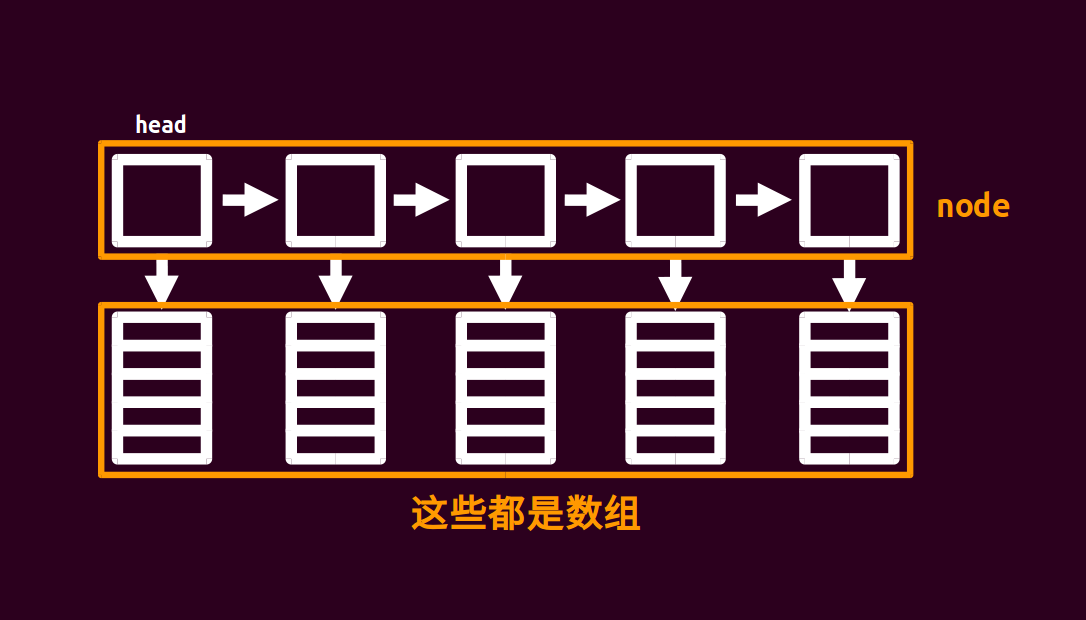
\includegraphics[width=0.7\textwidth]{docs/ds/images/kuaizhuanglianbiao.png} 
\caption{./images/kuaizhuanglianbiao.png}
\end{figure} 

大概就长这样……

不难发现块状链表就是一个链表,每个节点指向一个数组。

我们把原来长度为 n 的数组分为 $\sqrt{n}$ 个节点,每个节点对应的数组大小为 $\sqrt{n}$ 。

所以我们这么定义结构体,代码见下。

其中 \texttt{sqn} 表示 \texttt{sqrt(n)} 即 $\sqrt{n}$,\texttt{pb} 表示 \texttt{push\_back},即在这个 \texttt{node} 中加入一个元素。

\begin{cppcode}
struct node {
  node* nxt;
  int size;
  char d[(sqn << 1) + 5];
  node() { size = 0, nxt = NULL, memset(d, 0, sizeof(d)); }
  void pb(char c) { d[size++] = c; }
};
\end{cppcode}

块状链表应该至少支持:分裂、插入、查找。

什么是分裂?分裂就是分裂一个 \texttt{node},变成两个小的 \texttt{node},以保证每个 \texttt{node} 的大小都接近 $\sqrt{n}$ (否则可能退化成普通数组)。当一个 \texttt{node} 的大小超过 $2\times \sqrt{n}$ 时执行分裂操作。

分裂操作怎么做呢?先新建一个节点,再把被分裂的节点的后 $\sqrt{n}$ 个值 \texttt{copy} 到新节点,然后把被分裂的节点的后 $\sqrt{n}$ 个值删掉(\texttt{size--}),最后把新节点插入到被分裂节点的后面即可。

块状链表的所有操作的复杂度都是 $\sqrt{n}$ 的。

还有一个要说的。

随着元素的插入(或删除),$n$ 会变, $\sqrt{n}$ 也会变。这样块的大小就会变化,我们难道还要每次维护块的大小?

其实不然,把 $\sqrt{n}$ 设置为一个定值即可。比如题目给的范围是 $10^6$,那么 $\sqrt{n}$ 就设置为大小为 $10^3$ 的常量,不用更改它。

\begin{cppcode}
list<vector<char> > orz_list;
\end{cppcode}

\subsection{例题}

Big String POJ - 2887

题解:

很简单的模板题。代码如下:

\begin{cppcode}
#include <cctype>
#include <cstdio>
#include <cstring>
using namespace std;
static const int sqn = 1e3;
struct node {
  node* nxt;
  int size;
  char d[(sqn << 1) + 5];
  node() { size = 0, nxt = NULL; }
  void pb(char c) { d[size++] = c; }
}* head = NULL;
char inits[(int)1e6 + 5];
int llen, q;
void readch(char& ch) {
  do
    ch = getchar();
  while (!isalpha(ch));
}
void check(node* p) {
  if (p->size >= (sqn << 1)) {
    node* q = new node;
    for (int i = sqn; i < p->size; i++) q->pb(p->d[i]);
    p->size = sqn, q->nxt = p->nxt, p->nxt = q;
  }
}
void insert(char c, int pos) {
  node* p = head;
  int tot, cnt;
  if (pos > llen++) {
    while (p->nxt != NULL) p = p->nxt;
    p->pb(c), check(p);
    return;
  }
  for (tot = head->size; p != NULL && tot < pos; p = p->nxt, tot += p->size)
    ;
  tot -= p->size, cnt = pos - tot - 1;
  for (int i = p->size - 1; i >= cnt; i--) p->d[i + 1] = p->d[i];
  p->d[cnt] = c, p->size++;
  check(p);
}
char query(int pos) {
  node* p;
  int tot, cnt;
  for (p = head, tot = head->size; p != NULL && tot < pos;
       p = p->nxt, tot += p->size)
    ;
  tot -= p->size;
  return p->d[pos - tot - 1];
}
int main() {
  scanf("%s %d", inits, &q), llen = strlen(inits);
  node* p = new node;
  head = p;
  for (int i = 0; i < llen; i++) {
    if (i % sqn == 0 && i) p->nxt = new node, p = p->nxt;
    p->pb(inits[i]);
  }
  char a;
  int k;
  while (q--) {
    readch(a);
    if (a == 'Q')
      scanf("%d", &k), printf("%c\n", query(k));
    else
      readch(a), scanf("%d", &k), insert(a, k);
  }
  return 0;
}
\end{cppcode}

  \section{块状数组}
  


  \section{树分块}
  


\section{单调栈}

\subsection{何为单调栈}

顾名思义,单调栈即满足单调性的栈结构。与单调队列相比,其只在一端进行进出。

为了描述方便,以下举例及伪代码以维护一个整数的单调递增栈为例。

\subsection{如何使用单调栈}

\subsubsection{插入}

将一个元素插入单调栈时,为了维护栈的单调性,需要在保证将该元素插入到栈顶后整个栈满足单调性的前提下弹出最少的元素。

例如,栈中自顶向下的元素为 ${1,3,5,10,30,50}$,插入元素 $20$ 时为了保证单调性需要依次弹出元素 $1,3,5,10$,操作后栈变为 $20,30,50$。

用伪代码描述如下:

\begin{minted}{text}
insert x
while !sta.empty() && sta.top()<x
    sta.pop()
sta.push(x)
\end{minted}

\subsubsection{使用}

自然就是从栈顶读出来一个元素,该元素满足单调性的某一端。

例如举例中取出的即栈中的最小值。

\subsection{应用}

\begin{NOTE}{\href{http://poj.org/problem?id=3250}{POJ3250 Bad Hair Day}}{}
有 $N$ 头牛从左到右排成一排,每头牛有一个高度 $h_i$,设左数第 $i$ 头牛与「它右边第一头高度 $≥h_i$」的牛之间有 $c_i$ 头牛,试求 $\sum_{i=1}^{N} c_i$。

(可以左转 \href{https://www.luogu.org/problemnew/show/P2866}{洛谷 P2866})

\end{NOTE}


比较基础的应用有这一题,就是个单调栈的简单应用,记录每头牛被弹出的位置,如果没有被弹出过则为最远端,稍微处理一下即可计算出题目所需结果。

\section{单调队列}

在学习单调队列前,让我们先来看一道例题

\subsection{例题}

\href{http://poj.org/problem?id=2823}{Sliding Window}

本题大意是给出一个长度为 $n$ 的数组,编程输出每 $k$ 个连续的数中的最大值和最小值

最常用(\sout{暴力})的想法很简单,对于每一段 $i \sim i+k-1$ 的序列,逐个比较来找出最大值(和最小值),时间复杂度约为 $O(n \times k)$ 。

很显然,这其中进行了大量重复工作,除了开头 $k-1$ 个和结尾 $k-1$ 个数之外,每个数都进行了 $k$ 次比较,而题中 $100\%$ 的数据为 $n \le 1000000$ ,当 $k$ 稍大的情况下,显然会出现 TLE

这时所用到的就是单调队列了

\subsection{概念}

顾名思义,单调队列的重点分为 "单调" 和 "队列"

"单调" 指的是元素的的 "规律"——递增 (或递减)

"队列" 指的是元素只能从队头和队尾进行操作

Ps. 单调队列中的 "队列" 与正常的队列有一定的区别,稍后会提到

\subsection{例题分析}

有了上面 "单调队列" 的概念,很容易想到用单调队列进行优化

要求的是每连续的 $k$ 个数中的最大(最小)值,很明显,当一个数进入所要 "寻找" 最大值的范围中时,若这个数比其前面(先进队)的数要大,显然,前面的数会比这个数先出队且不再可能是最大值

也就是说——当满足以上条件时,可将前面的数 "弹出",再将该数真正 push 进队尾

这就相当于维护了一个递减的队列,符合单调队列的定义,减少了重复的比较次数,不仅如此,由于维护出的队伍是查询范围内的且是递减的,队头必定是该查询区域内的最大值,因此输出时只需输出队头即可

显而易见的是,在这样的算法中,每个数只要进队与出队各一次,因此时间复杂度被降到了 $O(N)$

而由于查询区间长度是固定的,超出查询空间的值再大也不能输出,因此还需要 site 数组记录第 $i$ 个队中的数在原数组中的位置,以弹出越界的队头

\href{https://www.luogu.org/paste/dze1lw3b}{例题代码}

Ps. 此处的 "队列" 跟普通队列的一大不同就在于可以从队尾进行操作, C++ 中有相似的数据结构 deque

\section{倍增}

倍增法,通过字面意思来看就是翻倍。这个方法在很多算法中均有应用。其中最常用的就是 RMQ 问题和求 LCA 了。

\subsection{RMQ 问题}

\subsubsection{简介}

RMQ 是英文 Range Maximum / Minimum Query 的缩写,表示区间最大(最小)值。

解决 RMQ 问题的主要方法有两种,分别是 ST 表和线段树。本文主要讲 ST 表。

\subsubsection{引入}

\href{https://www.luogu.org/problemnew/show/P3865}{ST 表模板题}

题目大意:给定 $n$ 个数,有 $m$ 个询问,对于每个询问,你需要回答区间 $[x,y]$ 中的最大值

考虑暴力做法。每次都对区间 $[x,y]$ 扫描一遍,求出最大值

显然,这个算法会超时

\subsubsection{ST 表}

$ST$ 表基于倍增思想,可以做到 $O(n\log n)$ 预处理,$O(1)$ 回答每个询问。但是不支持修改操作。

暴力跑的慢的原因在于检索了每一个点。

但是,如果我们预处理出每一段的最大值,就可以将效率提高很多。

令 $f[i][j]$ 表示 $[i,i+2^j-1]$ 的最大值。

显然,$f[i][0]=a[i]$

根据定义式,写出状态转移方程:$f[i][j]=\max(f[i][j-1],f[i+2^{j-1}][j-1])$

我们可以这么理解:将区间 $[i,i+2^j-1]$ 分成相同的两部分

中点即为 $(i+(i+2^j-1))/2=i+2^{j-1}-1/2$

所以 $[i,i+2^j-1]$ 可以分成 $[i,i+2^{j-1}-1]$ 和 $[i+2^{j-1}+1,i+2^j-1]$

\begin{figure}[htbp]
\centering
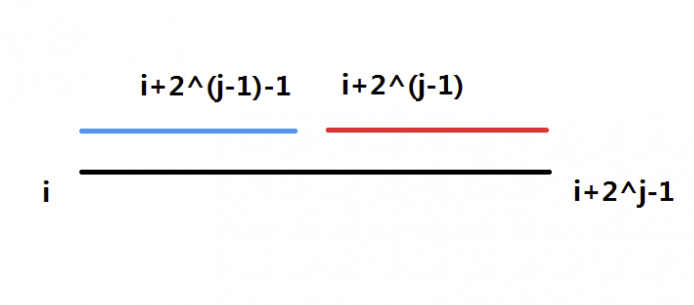
\includegraphics[width=0.7\textwidth]{docs/ds/images/st1.png} 

\end{figure}

预处理终于完成了!接下来就是查询了

对于每个询问 $[x,y]$,我们把它分成两部分

$f[x][s]$  $f[y-2^s+1][s]$

其中 $s=\log_2{(y-x+1)}$

显然,这两个区间会重叠。但是,重叠并不会对区间最大值产生影响。同时这两个区间刚好覆盖了 $[x,y]$,可以保证答案的正确性。

\subsubsection{模板代码}

\href{https://www.luogu.org/problemnew/show/P3865}{ST 表模板题}

\begin{cppcode}
#include <bits/stdc++.h>
using namespace std;
const int logn = 21;
const int maxn = 2000001;
long long a[maxn], f[maxn][logn], Logn[maxn];
inline int read() {
  char c = getchar();
  int x = 0, f = 1;
  while (c < '0' || c > '9') {
    if (c == '-') f = -1;
    c = getchar();
  }
  while (c >= '0' && c <= '9') {
    x = x * 10 + c - '0';
    c = getchar();
  }
  return x * f;
}
void pre() {
  Logn[1] = 0;
  Logn[2] = 1;
  for (int i = 3; i <= maxn; i++) {
    Logn[i] = Logn[i / 2] + 1;
  }
}
int main() {
  int n = read(), m = read();
  for (int i = 1; i <= m; i++) f[i][0] = read();
  pre();
  for (int j = 1; j <= logn; j++)
    for (int i = 1; i + (1 << j) - 1 <= n; i++)
      f[i][j] = max(f[i][j - 1], f[i + (1 << (j - 1))][j - 1]);
  for (int i = 1; i <= m; i++) {
    int x = read(), y = read();
    int s = Logn[y - x + 1];
    printf("%d\n", max(f[x][s], f[y - (1 << s) + 1][s]));
  }
  return 0;
}
\end{cppcode}

\subsubsection{注意点}

\begin{enumerate}
\item 输入输出数据一般很多,建议开启输入输出优化
\item 每次用 \href{https://en.cppreference.com/w/cpp/numeric/math/log}{std::log} 重新计算 log 函数值并不值得,建议如下预处理
\end{enumerate}

$$
\left\{\begin{aligned}
Logn[1] &=0, \\
Logn\left[i\right] &=Logn[\frac{i}{2}] + 1.
\end{aligned}\right.
$$

\subsubsection{总结}

$ST$ 表能较好的维护区间信息,时间复杂度较低,代码量相对其他算法不大。但是,$ST$ 表能维护的信息非常有限,不能较好地扩展,并且不支持修改操作。

\subsection{树上倍增求 LCA}

\subsubsection{LCA 简介}

LCA(Least Common Ancestors)表示最近公共祖先。

对于一棵有根树,设 $LCA(u,v)=x$,则 $x$ 必须满足以下条件

\begin{itemize}
\item $x$ 是 u 的祖先或 u
\item $x$ 是 v 的祖先或 v
\item $x$ 是在满足上面两个条件下深度最大的
\end{itemize}

显然,在一棵有根树内,对于任意两个节点有且仅有一个 $LCA$

解决这个问题,我们通常有以下方法

\begin{itemize}
\item 树上倍增(本文主要讲解此方法)
\item 转化为 RMQ 问题
\item 树链剖分
\item Tarjan
\end{itemize}

\subsubsection{暴力做法}

\begin{enumerate}
\item 将两个点跳到同一深度
将深度大的点 \textbf{ 一步一步 } 往上跳,发现另一个点是他的祖先,则另一个点就是 $LCA$
\item 一起往上跳
当两个点深度一样但是还没有找到 LCA 的时候,就一起往 \textbf{ 一步一步 } 上跳,知道跳到了同一个点。那么,这个点即为它们的 LCA
\end{enumerate}

\subsubsection{树上倍增}

暴力慢的原因在于跳的时候是 \textbf{ 一步一步 } 跳的,导致效率较低。如果我们可以 \textbf{ 一次跳多步 },效率就大大提高了。

\paragraph{预处理}

令 $f[i][j]$ 表示 $i$ 的 $2^j$ 辈祖先,及从 $i$ 向根节点走 $2^j$ 步到达的节点。$f[i][0]$ 就表示 $i$ 的父节点。

通过 $2^{j-1}\times 2^{j-1}=2^j$ 可以得到状态转移方程 $f[i][j]=f[f[i][j-1]][j-1]$\sout{(是不是和 $ST$ 的转移方程有点像)}。自然,当 $i$ 没有 $2^j$ 辈祖先时 $f[i][j]=0$

一遍 DFS 计算即可

\begin{cppcode}
void dfs(int u, int father) {
  dep[u] = dep[father] + 1;  // dep[x] 表示 x 的深度,在查询时会用到
  for (int i = 0; i <= 19; i++) f[u][i + 1] = f[f[u][i]][i];  // 预处理
  for (int i = first[u]; i; i = next[i])                      // 链式前向星
  {
    int v = go[i];
    if (v == father) continue;
    f[v][0] = u;  // f[v][0] 表示 v 的父亲
    dfs(v, u);
  }
}
\end{cppcode}

\paragraph{查询}

依然采用暴力的思想。先将两个节点跳到同一深度,然后一起往上跳。

只不过在跳的过程中从一步一步跳变成了 \textbf{ 一次跳多步 }。可以具体分为以下几步

\begin{enumerate}
\item 让 $x$ 的深度比 $y$ 大(深度在预处理时已经求出)
\item 将两个节点跳到同一深度。在此处我们使用二进制思想,依次尝试向上跳 $2^i,2^{i-1}\cdots 2^1,2^0$。如果发现则 $x$ 跳到了 $y$ 就说明 $LCA(x,y)=y$
\item 一起往上跳。依然使用二进制思想,让他们一起往上跳 $2^i,2^{i-1}\cdots 2^1,2^0$. 如果 $f[x][i]!=f[y][i]$,说明 $x$ 和 $y$ 还未相遇。最后,$x$ 和 $y$ 必定只差一步相遇。这时 $x$ 的父亲即 $f[x][0]$ 就是他们的 LCA
\end{enumerate}

\begin{cppcode}
int lca(int x, int y) {
  if (dep[x] < dep[y]) swap(x, y);  // 步骤 1
  for (int i = 20; i >= 0; i--)     // 步骤 2
  {
    if (dep[f[x][i]] >= dep[y]) x = f[x][i];
    if (x == y) return x;
  }
  for (int i = 20; i >= 0; i--)  // 步骤 3
    if (f[x][i] != f[y][i]) {
      x = f[x][i];
      y = f[y][i];
    }
  return f[x][0];
}
\end{cppcode}

\subsubsection{总结}

树上倍增法可以在 $O(n\log n)$ 的时间内完成预处理,在 $O(\log n)$ 的时间里完成查询,是一个较高效的算法,代码量也不大,一般竞赛推荐使用。

\subsection{练习}

\href{https://www.luogu.org/problemnew/show/P3865}{RMQ 模板题}

\href{https://www.luogu.org/problemnew/show/P3379}{LCA 模板题}

\href{https://www.luogu.org/problemnew/show/P4180}{严格次小生成树}

\href{https://www.luogu.org/problemnew/show/P1967}{货车运输}

\href{https://www.luogu.org/problemnew/show/P1613}{跑路}

\section{树状数组}

\subsection{简介}

\hr

树状数组和下面的线段树可是亲兄弟了,但他俩毕竟还有一些区别:  

树状数组能有的操作,线段树一定有;  

线段树有的操作,树状数组不一定有。

这么看来选择线段树不就\textbf{「得天下了」}?

事实上,树状数组的代码要比线段树短得多,思维也更清晰,在解决一些单点修改的问题时,树状数组是不二之选。

\hr

\subsection{原理}

如果要具体了解树状数组的工作原理,请看下面这张图:

\begin{figure}[htbp]
\centering
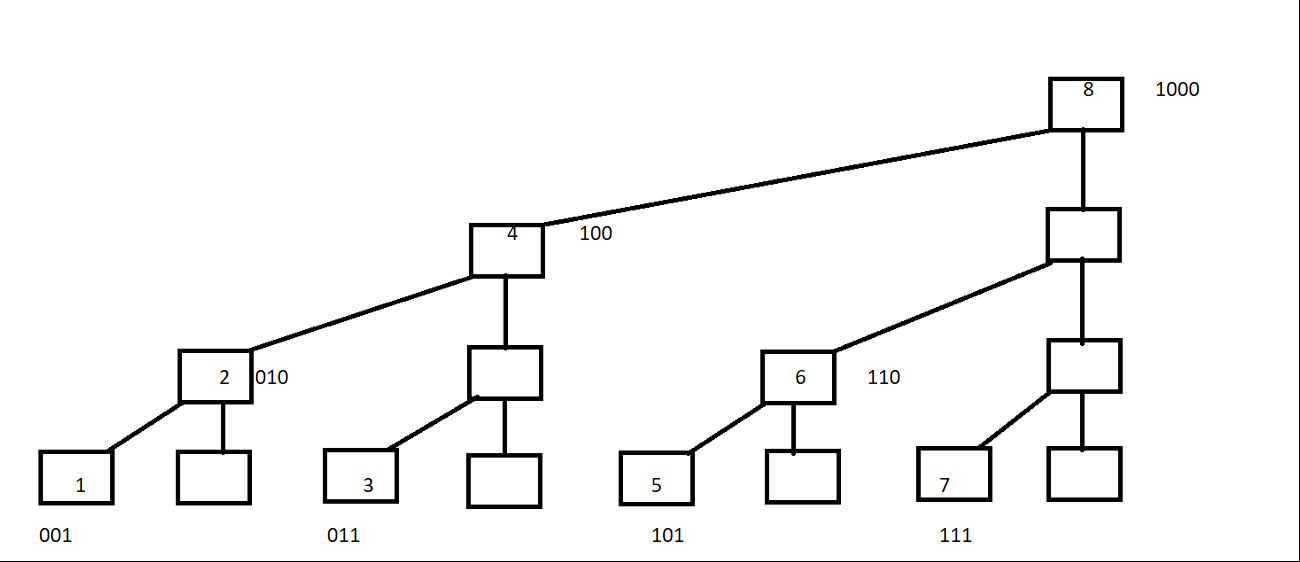
\includegraphics[width=0.7\textwidth]{docs/ds/images/bit1.png} 

\end{figure}

最下面的八个方块就代表存入 $a$ 中的八个数,现在都是十进制。

他们上面的参差不齐的剩下的方块就代表 $a$ 的上级——$c$ 数组。

很显然看出:  

$c[2]$ 管理的是 $a[1]$ \& $a[2]$ ;  

$c[4]$ 管理的是 $a[1]$ \& $a[2]$ \& $a[3]$ \& $a[4]$ ;  

$c[6]$ 管理的是 $a[5]$ \& $a[6]$ ;$c[8]$ 则管理全部 $8$ 个数。

所以,如果你要算区间和的话,比如说要算 $a[51]$ \textasciitilde{} $a[91]$ 的区间和,暴力算当然可以,那上百万的数,那就 RE 喽。

那么这种类似于跳一跳的连续跳到中心点而分值不断变大的原理是一样的(倍增)。

你从 $91$ 开始往前跳,发现 $c[n]$($n$ 我也不确定是多少,算起来太麻烦,就意思一下)只管 $a[91]$ 这个点,那么你就会找 $a[90]$,发现 $c[n - 1]$ 管的是 $a[90]$ \& $a[89]$ ;那么你就会直接跳到 $a[88]$ ,$c[n - 2]$ 就会管 $a[81]$ \textasciitilde{} $a[88]$ 这些数,下次查询从 $a[80]$ 往前找,以此类推。

\hr

\subsection{用法及操作}

那么问题来了,你是怎么知道 $c$ 管的 $a$ 的个数分别是多少呢?你那个 $1$ 个,$2$ 个,$8$ 个…… 是怎么来的呢?

这时,我们引入一个函数—— \texttt{lowbit}:

\begin{cppcode}
int lowbit(int x) {
  //算出x二进制的从右往左出现第一个1以及这个1之后的那些0组成数的二进制对应的十进制的数
  return x & -x;
}
\end{cppcode}

\texttt{lowbit} 的意思注释说明了,咱们就用这个说法来证明一下 $a[88]$:  

$88_{(10)}=1011000_{(2)}$  

发现第一个 $1$ 以及他后面的 $0$ 组成的二进制是 $1000$  

$1000_{(2)} = 8_{(10)}$  

$1000$ 对应的十进制是 $8$,所以 $c$ 一共管理 $8$ 个 $a$。

这就是 \texttt{lowbit} 的用处,仅此而已(但也相当有用)。

\textbf{你可能又问了:x \& -x 是什么意思啊?}

\begin{QUOTE}{}{}
$-x$ 代表 $x$ 的负数,计算机中负数使用对应的正数的补码来表示。
\end{QUOTE}

例如 :  

$x =88_{(10)}=1011000_{(2)}$;  

$-x = -88_{(10)} = (0100111_{(2)} + 1_{(2)}) =101000_{(2)}$;  

$x\ \& \ (-x) = 1000_{(2)} = 8_{(10)}$。

神奇吧,我也觉得神奇!

那么对于\textbf{单点修改}就更轻松了:

\begin{cppcode}
void change(int x, int k) {
  while (x <= n)  //不能越界
  {
    c[x] = c[x] + k;
    x = x + lowbit(x);
  }
}
\end{cppcode}

每次只要在他的上级那里更新就行,自己就可以不用管了。

\begin{cppcode}
int getsum(int x)  // a[1]……a[x]的和
{
  int ans = 0;
  while (x >= 1) {
    ans = ans + c[x];
    x = x - lowbit(x);
  }
  return ans;
}
\end{cppcode}

\textbf{区间和}也不用说了吧,代码十分清真。

\subsection{例题}

\href{https://www.luogu.org/problemnew/show/P3374}{传送门}  

\href{https://www.luogu.org/problemnew/show/P3368}{传送门 2}

\section{线段树}

\subsection{1. 写在前面}

线段树是个好东西啊 QwQ

OI 中最常用的数据结构之一,不学不行啊 OvO

\subsection{2. 线段树是什么}

\begin{QUOTE}{}{}
线段树是一种二叉搜索树,与区间树相似,它将一个区间划分成一些单元区间,每个单元区间对应线段树中的一个叶结点。使用线段树可以快速的查找某一个节点在若干条线段中出现的次数,时间复杂度为 $O(\log N)$。而未优化的空间复杂度为 $2N$,因此有时需要离散化让空间压缩。——From 度娘
\end{QUOTE}

反正就是一种可以在很短的时间内对某个区间进行操作的数据结构。

\subsection{3. 线段树有什么用}

在 $O(\log N)$ 的时间复杂度内实现如:单点修改、区间修改、区间查询(如:区间求和,求区间最大值,求区间最小值……)还有很多……

总之线段树维护的信息,需要满足可加性,且要以可以接受的速度合并信息和修改信息,如果使用标记,标记也要满足可加性(例如取模就不满足可加性,对 $4$ 取模然后对 $3$ 取模,两个操作就不能合并在一起做(事实上某些情况下可以暴力单点取模))

\subsection{4. 线段树怎么实现}

\subsubsection{(1) 线段树的基本结构与建树}

想要建立一棵线段树,不理解它的结构、原理是肯定行不通的。

下面我来举个栗子:

我们有个大小为 $5$ 的数组 $a=\{10,11,12,13,14\}$ 要进行区间求和操作,现在我们要怎么把这个数组存到线段树中(也可以说是转化成线段树)呢?我们这样子做:设线段树的根节点编号为 $1$,用数组 $d$ 来保存我们的线段树,$d[i]$ 用来保存编号为 $i$ 的节点的值(这里节点的值就是这个节点所表示的区间总和),如图所示:

\begin{figure}[htbp]
\centering
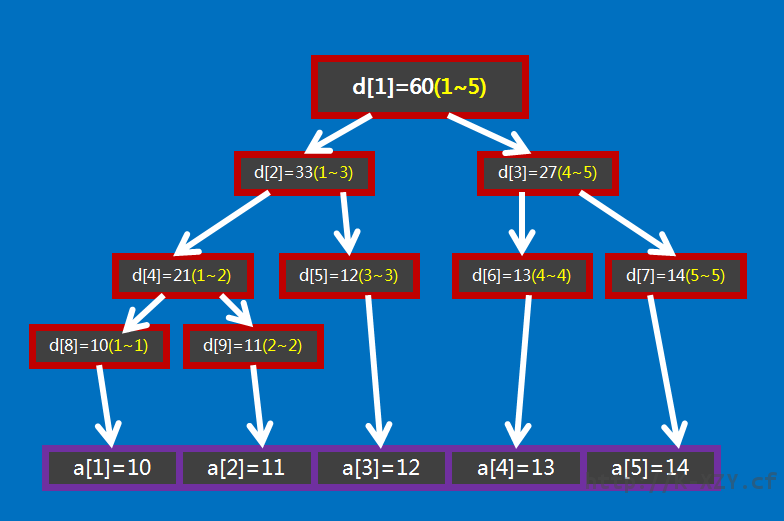
\includegraphics[width=0.7\textwidth]{docs/ds/images/segt1.png} 

\end{figure}

图中 $d[1]$ 表示根节点,紫色方框是数组 $a$,红色方框是数组 $d$,红色方框中的括号中的黄色数字表示它所在的那个红色方框表示的线段树节点所表示的区间,如 $d[1]$ 所表示的区间就是 $1\sim 5\ (a[1]\sim a[5])$,即 $d[1]$ 所保存的值是 $a[1]+a[2]+ \cdots +a[5]$,$d[1]=60$ 表示的是 $a[1]+a[2]+ \cdots +a[5]=60$。

通过观察我们不难发现,$d[i]$ 的左儿子节点就是 $d[2\times i]$,$d[i]$ 的右节点就是 $d[2\times i+1]$。进一步观察,可以看出如果 $d[i]$ 表示的是区间 $[s,t]$(即 $d[i]=a[s]+a[s+1]+ \cdots +a[t]$ ) 的话,那么 $d[i]$ 的左儿子节点表示的是区间 $[s, \frac{s+t}{2} ]$,$d[i]$ 的右儿子表示的是区间 $[ \frac{s+t}{2} +1,t]$。

为什么要这样表示呢?因为线段树利用了二分的思想,线段树实际上是个二叉树,这些不懂的话就无法理解线段树了,所以如果不明白二分或者二叉树的话…… 建议去问问度娘。

具体要怎么用代码实现呢?

我们继续观察,有没有发现如果 $d[i]$ 表示的区间大小等于 $1$(区间大小指的是区间包含的元素的个数,即 $a$ 的个数)的话(设 $d[i]$ 表示区间 $[s,t]$,它的区间大小就是 $t-s+1$,不信你看上面的图),那么 $d[i]$ 所表示的区间 $[s,t]$ 中 $s$ 肯定等于 $t$(不信你还是看图),且 $d[i]=a[s]$(当然也等于 $a[t]$)。

为什么要讲这个东西呢?你没发现这个是个递归边界吗?

O(∩\textbackslash{}\_∩)O 哈哈\textasciitilde{}

\textbf{ 思路如下:}

\begin{figure}[htbp]
\centering
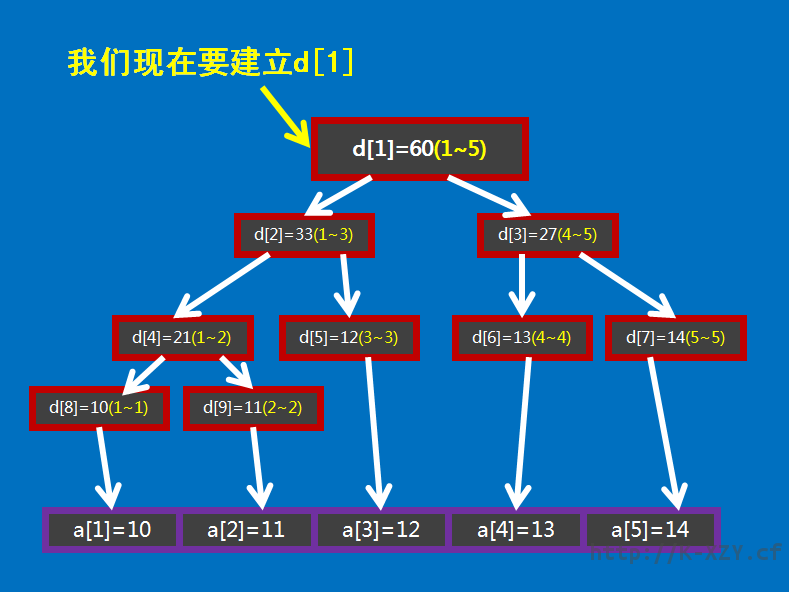
\includegraphics[width=0.7\textwidth]{docs/ds/images/segt2.png} 

\end{figure}

\begin{figure}[htbp]
\centering
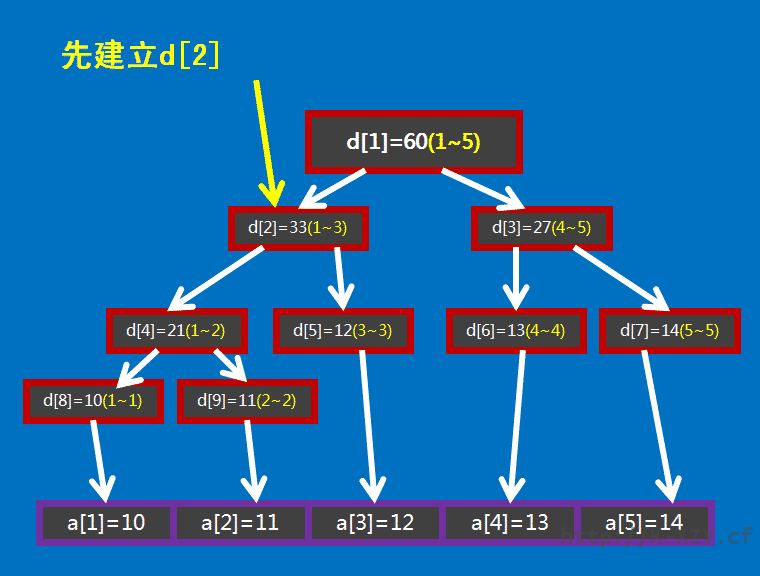
\includegraphics[width=0.7\textwidth]{docs/ds/images/segt3.png} 

\end{figure}

\begin{figure}[htbp]
\centering
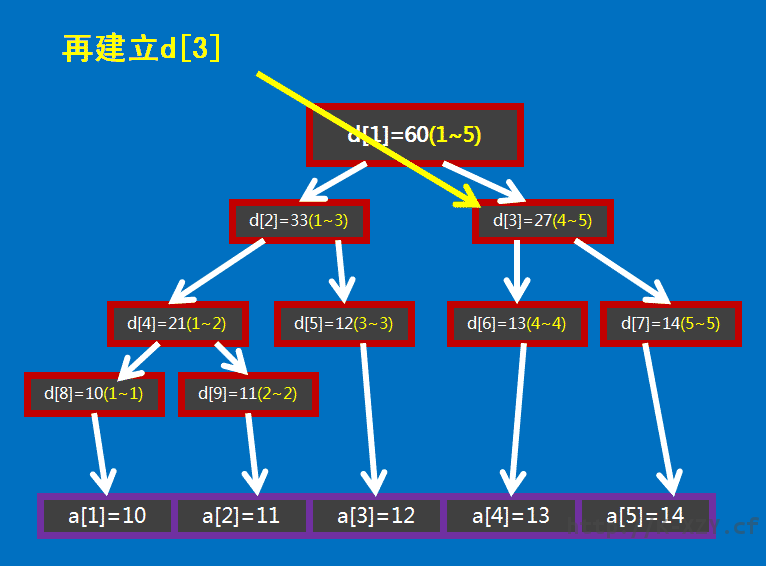
\includegraphics[width=0.7\textwidth]{docs/ds/images/segt4.png} 

\end{figure}

那么就这样写代码:

\begin{cppcode}
建树(s, t, i) {
  如果(s == t) { d[i] = a[s]; }
  否则 {
    建树(s, (s + t) / 2, 2 * i);
    建树((s + t) / 2 + 1, t, 2 * i + 1);
    d[i] = d[2 * i] + d[2 * i + 1];
  }
}
\end{cppcode}

具体代码实现 (C++):

\begin{cppcode}
void build(int s, int t, int p) {
  if (s == t) {
    d[p] = a[s];
    return;
  }
  int m = (s + t) / 2;
  build(s, m, p * 2), build(m + 1, t, p * 2 + 1);
  d[p] = d[p * 2] + d[(p * 2) + 1];
}
\end{cppcode}

上面那短短 $7$ 行代码就能建立一个线段树。

关于线段树的空间,如果采用堆式存储(上面的代码就是堆式存储,即 $2\times p$ 是 p 的左儿子,$2 \times p+1$ 是 p 的右儿子),d 数组的大小需要是 $n$ (元素个数)上取到一个 $2$ 的整数次幂(叶子数量)再乘以 $2$(叶子上面的节点数量),上界是 $4$ 倍,可利用上面的 build 自行验证,如果采用动态开点,则需要两倍的空间(需要额外地记录左儿子和右儿子的编号 / 地址)。

\begin{figure}[htbp]
\centering
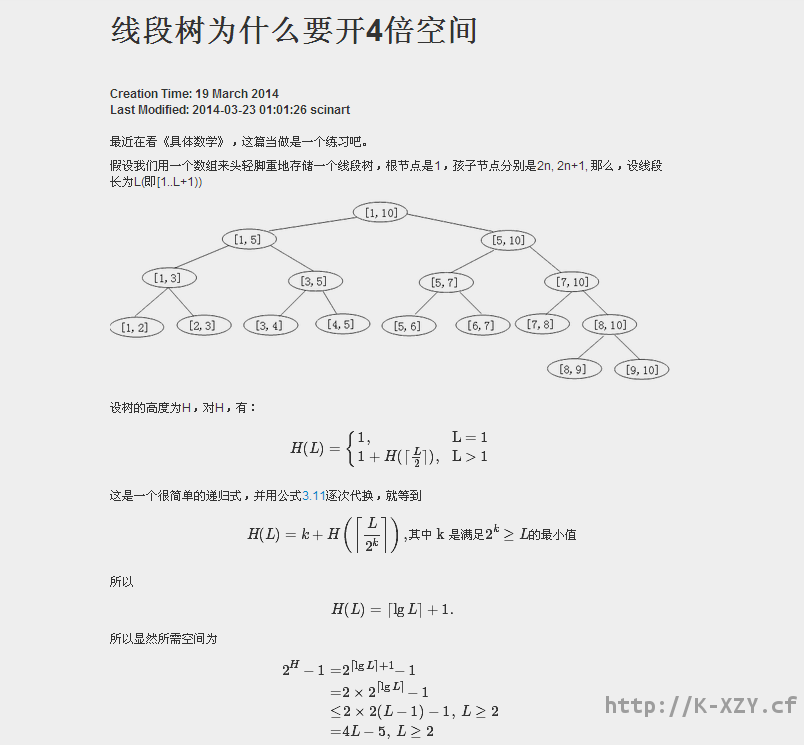
\includegraphics[width=0.7\textwidth]{docs/ds/images/segt5.png} 

\end{figure}

\subsubsection{(2) 线段树的区间查询}

区间查询,比如求区间 $[l,r]$ 的总和(即 $a[l]+a[l+1]+ \cdots +a[r]$)、求区间最大值 / 最小值…… 还有很多很多…… 怎么做呢?

\begin{figure}[htbp]
\centering
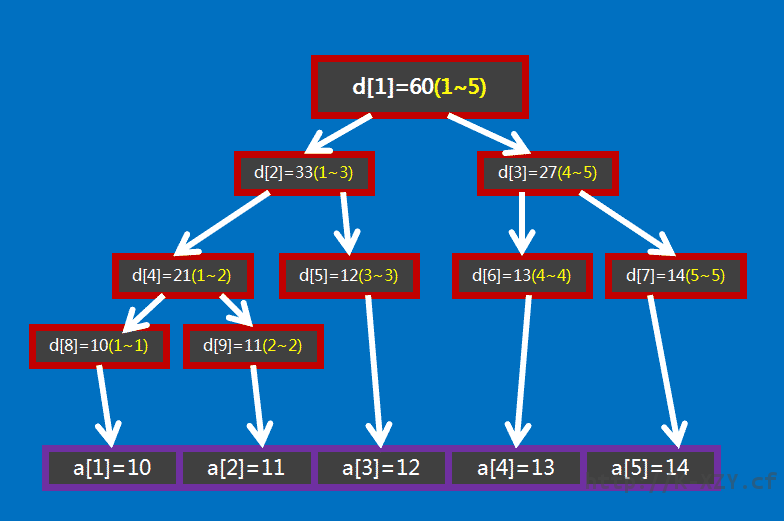
\includegraphics[width=0.7\textwidth]{docs/ds/images/segt6.png} 

\end{figure}

拿上面这张图举栗!

\begin{figure}[htbp]
\centering

\includegraphics[width=0.7\textwidth]{docs/ds/images/segt7.png} 

\end{figure}

(发博客累死了无聊一下)

如果要查询区间 $[1,5]$ 的和,那直接获取 $d[1]$ 的值($60$)即可。那如果我就不查询区间 $[1,5]$,我就查区间 $[3,5]$ 呢?

\textbf{Σ(⊙▽⊙"a}

懵 B 了吧。但其实呢我们肯定还是有办法的!

\textbf{\&lt;( ̄ˇ ̄)/}

你要查的不是 $[3,5]$ 吗?我把 $[3,5]$ 拆成 $[3,3]$ 和 $[4,5]$ 不就行了吗?

具体思路见代码:

\begin{cppcode}
求和(查询区间的左端点 l, 查询区间的右端点 r, 当前节点表示的区间左端点 s,
    当前节点表示的区间 t, 当前访问的节点编号 p) {
  如果(l <= s&& t <= r)  // 当前访问的节点表示的区间包含在查询区间内
      {返回 d[p] ;} 否则 {
    令 返回值 = 0 如果(l <=
                (s + t) / 2)  // 当前访问的节点的左儿子节点表示的区间包含在查
                               // 询区间内,(s+t)/2
                               // 其实是左右儿子节点表示的区间的分割线且(s+t)/2
                               // 包含在左儿子节点表示的区间中
    {
      返回值 += 求和(l, r, s, (s + t) / 2,
          p * 2);  // l 和 r
                    // 是可以不用变的!不管你信不信我反正是信了。当前节点的左儿子节点编号是
                    // p2,之前讲过了,左儿子节点表示的区间左端点就是当前节点表示的区间的左端点,(s+t)/2
                    // 是左儿子节点表示的区间的右短点
    }
    如果(r >
         (s + t) / 2)  // 当前访问的节点的右儿子节点表示的区间包含在查 询区间内
    {
        返回值 += 求和(l, r, (s + t) / 2 + 1, t,
        p * 2 + 1);  //(s+t)/2+1 是当前访问节点的右儿子节点表示的区间的左端点
    } 返回 返回值;
  }
}
\end{cppcode}

怎么样,代码很丑吧?废话,用中文写的能不丑吗?现在搞个英 (da) 文 (xin) 的 (wen):

\begin{cppcode}
int getsum(int l, int r, int s, int t, int p) {
  if (l <= s && t <= r) return d[p];
  int m = (s + t) / 2, sum = 0;
  if (l <= m) sum += getsum(l, r, s, m, p * 2);
  if (r > m) sum += getsum(l, r, m + 1, t, p * 2 + 1);
  return sum;
}
\end{cppcode}

还是挺短的吧?这里用到的主要思路就是把一个区间拆成左右两个区间,再分别处理左右区间。也是二分的思想。

\subsubsection{(3) 线段树的区间修改与懒惰标记}

区间修改是个很有趣的东西 o(╯□╰)o…… 你想啊,如果你要修改区间 $[l,r]$,难道把所有包含在区间 [l,r] 中的节点都遍历一次、修改一次?那估计这时间复杂度估计会上天 |(′口 )。这怎么办呢?我们这里要引用一个叫做 \textbf{「懒惰标记」} 的东西。

我们设一个数组 $b$,$b[i]$ 表示编号为 $i$ 的节点的懒惰标记值。啥是懒惰标记、懒惰标记值呢?(O\_O)? 这里我再举个栗子(原创小故事我真有才哈哈哈 (◡ᴗ◡✿)):

\begin{QUOTE}{}{}
A 有两个儿子,一个是 B,一个是 C。



有一天 A 要建一个新房子,没钱。刚好过年嘛,有人要给 B 和 C 红包,两个红包的钱数相同都是 $(1000000000000001\bmod 2)$ 圆(好多啊!…… 不就是 $1$ 元吗……),然而因为 A 是父亲所以红包肯定是先塞给 A 咯\textasciitilde{}



理论上来讲 A 应该把两个红包分别给 B 和 C,但是…… 缺钱嘛,A 就把红包偷偷收到自己口袋里了。



A 高兴♂地说:「我现在有 $2$ 份红包了!我又多了 $2\times (1000000000000001\bmod 2)=2$ 圆了!哈哈哈\textasciitilde{}」



但是 A 知道,如果他不把红包给 B 和 C,那 B 和 C 肯定会不爽然后导致家庭矛盾最后崩溃,所以 A 对儿子 B 和 C 说:「我欠你们每人 $1$ 份 $(1000000000000001\bmod 2)$ 圆的红包,下次有新红包给过来的时候再给你们!这里我先做下记录…… 嗯…… 我钱你们各 $(1000000000000001\bmod 2)$ 圆……」



儿子 B、C 有点恼怒:「可是如果有同学问起我们我们收到了多少红包咋办?你把我们的红包都收了,我们还怎么装 ×?」



父亲 A 赶忙说:「有同学问起来我就会给你们的!我欠条都写好了不会不算话的!」



这样 B、C 才放了心。



注:$\bmod$ 是取余数的意思,$a\bmod b$ 就是 $a$ 除以 $b$ 的余数,所以……$1000000000000001\bmod 2=1$。
\end{QUOTE}

在这个故事中我们不难看出,A 就是父亲节点,B 和 C 是 A 的儿子节点,而且 B 和 C 是叶子节点,分别对应一个数组中的值(就是之前讲的数组 $a$),我们假设节点 A 表示区间 $[1,2]$(即 $a[1]+a[2]$),节点 B 表示区间 $[1,1]$(即 $a[1]$),节点 C 表示区间 $[2,2]$(即 $a[2]$),它们的初始值都为 $0$(现在才刚开始呢,还没拿到红包,所以都没钱\textasciitilde{})。

如图:

\begin{figure}[htbp]
\centering
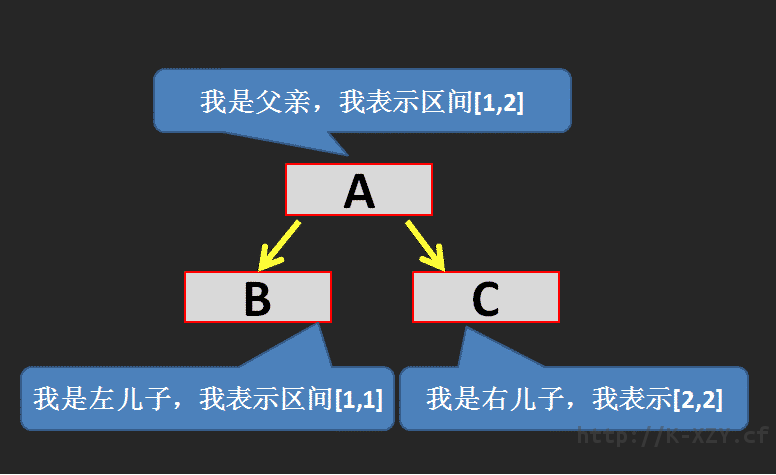
\includegraphics[width=0.7\textwidth]{docs/ds/images/segt8.png} 

\end{figure}

\begin{figure}[htbp]
\centering
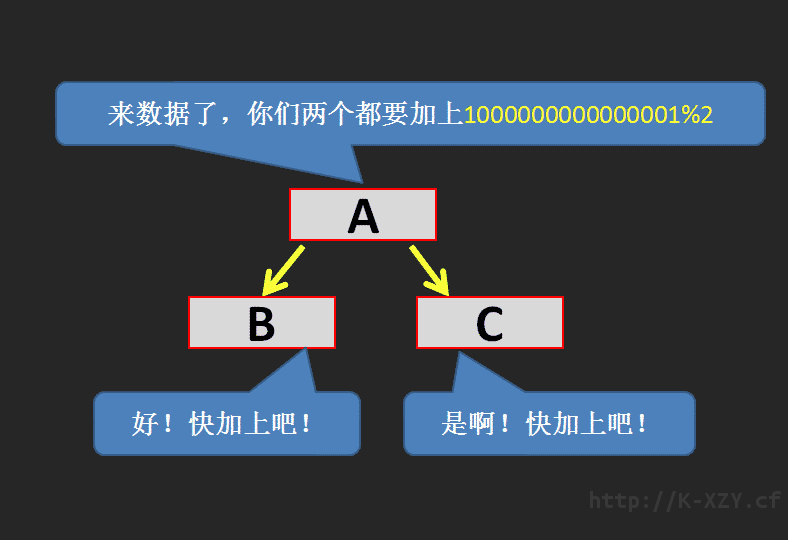
\includegraphics[width=0.7\textwidth]{docs/ds/images/segt9.png} 

\end{figure}

\begin{figure}[htbp]
\centering
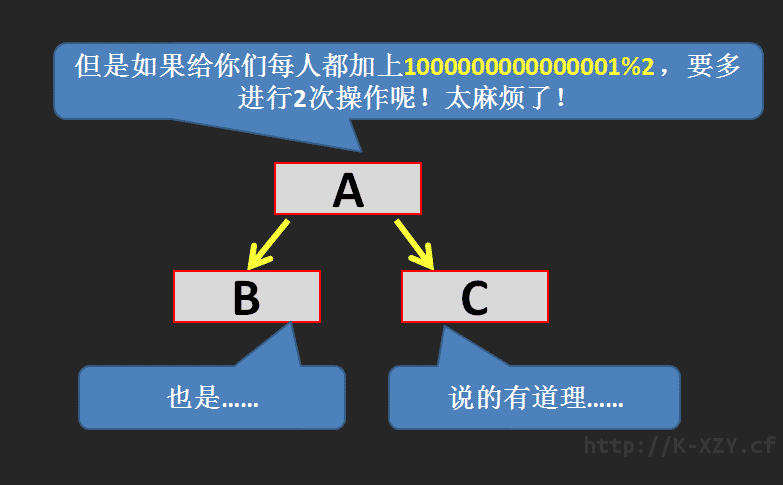
\includegraphics[width=0.7\textwidth]{docs/ds/images/segt10.png} 

\end{figure}

\begin{figure}[htbp]
\centering
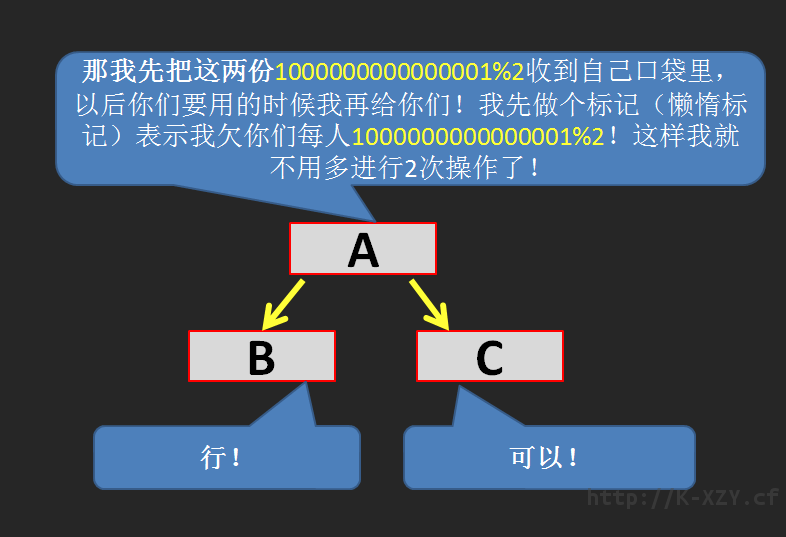
\includegraphics[width=0.7\textwidth]{docs/ds/images/segt11.png} 

\end{figure}

\begin{figure}[htbp]
\centering
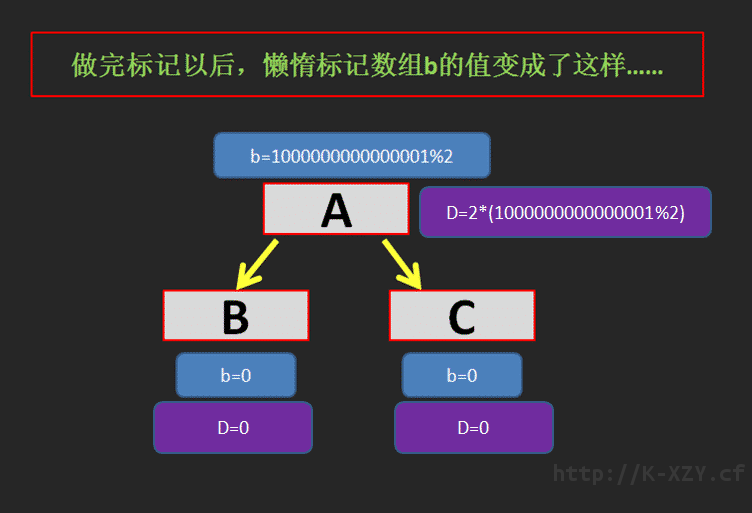
\includegraphics[width=0.7\textwidth]{docs/ds/images/segt12.png} 

\end{figure}

注:这里 D 表示当前节点的值(即所表示区间的区间和)。

为什么节点 A 的 D 是 $2\times (1000000000000001\bmod 2)$ 呢?原因很简单。节点 A 表示的区间是 $[1,2]$,一共包含 $2$ 个元素。我们是让 $[1,2]$ 这个区间的每个元素都加上 $1000000000000001\bmod 2$,所以节点 A 的值就加上了 $2\times (1000000000000001\bmod 2)$ 咯 = ̄ω ̄= 。

如果这时候我们要查询区间 $[1,1]$(即节点 B 的值)怎么办呢?不是说了吗?如果 B 要用到的时候,A 就把它欠的还给 B!

具体是这样操作(如图):

\begin{figure}[htbp]
\centering
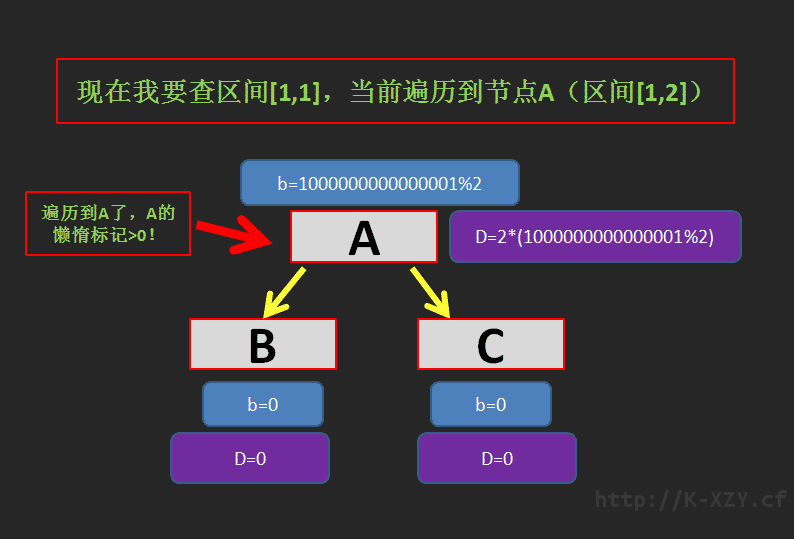
\includegraphics[width=0.7\textwidth]{docs/ds/images/segt13.png} 

\end{figure}

\begin{figure}[htbp]
\centering
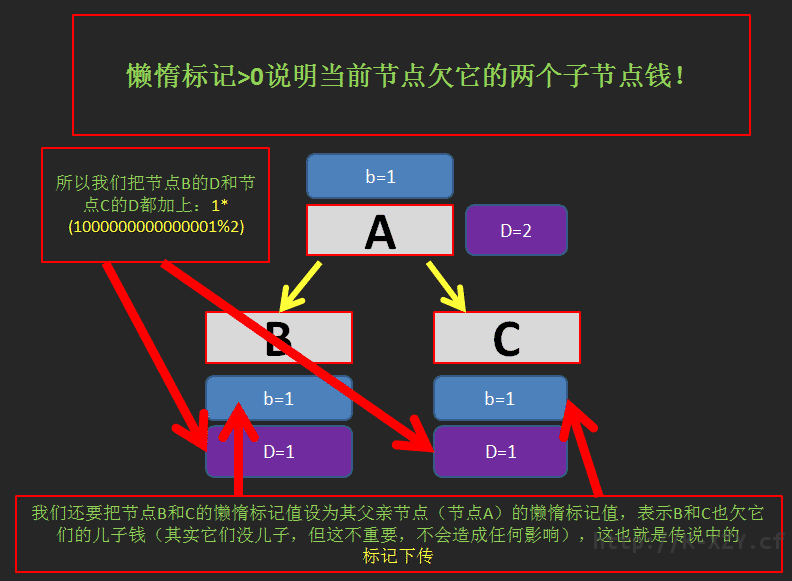
\includegraphics[width=0.7\textwidth]{docs/ds/images/segt14.png} 

\end{figure}

注:为什么是加上 $1\times (1000000000000001\bmod 2)$ 呢?

原因和上面一样——B 和 C 表示的区间中只有 $1$ 个元素啊!

\begin{figure}[htbp]
\centering
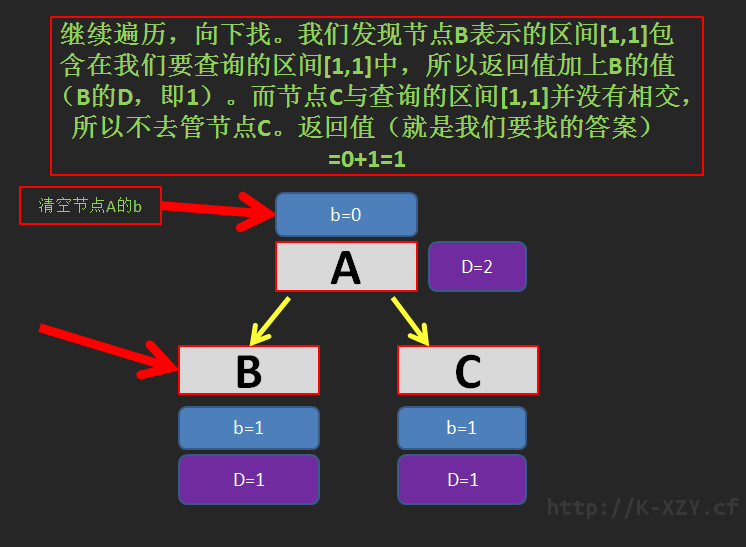
\includegraphics[width=0.7\textwidth]{docs/ds/images/segt15.png} 

\end{figure}

由此我们可以得到,区间 $[1,1]$ 的区间和就是 $1$ 啦!O(∩\textbackslash{}\_∩)O 哈哈\textasciitilde{}!

代码如下(下面代码不知道为什么显示出来很丑,建议复制到自己的 C++ 编辑器里看……):

区间修改(区间加上某个值):

\begin{cppcode}
void update(
    int l, int r, int c, int s, int t,
    int p)  // l 是查询的区间左端点,r 是右端点,c 表示区间每个元素加上的值,s
            // 是当前节点所表示的区间的左端点,t 是右端点,p
            // 是当前节点的编号(根节点标号为 1)
{
  if (l <= s && t <= r) {
    d[p] += (t - s + 1) * c, b[p] += c;
    return;
  }  // 如果当前节点表示的区间完全包含在查询区间内,直接修改当前节点的值,然后做上标记,结束修改
  int m = (s + t) / 2;  // 计算左右节点表示区间的分割线
  if (b[p] &&
      s !=
          t)  // 如果当前节点不是叶子节点(叶子节点表示的区间的左右端点是相等的)且当前的懒惰标记值!=0,就更新当前节点的两个儿子节点的值和懒惰标记值
    d[p * 2] += b[p] * (m - s + 1), d[p * 2 + 1] += b[p] * (t - m),
        b[p * 2] += b[p], b[p * 2 + 1] += b[p];
  b[p] = 0;  // 清空当前节点的懒惰标记值
  if (l <= m) update(l, r, c, s, m, p * 2);
  if (r > m) update(l, r, c, m + 1, t, p * 2 + 1);
  d[p] = d[p * 2] + d[p * 2 + 1];
}
\end{cppcode}

区间查询(求和):

\begin{cppcode}
int getsum(int l, int r, int s, int t,
           int p)  // l 是查询的区间左端点,r 是右端点,s
                   // 是当前节点所表示的区间的左端点,t 是右端点,p
                   // 是当前节点的编号(根节点标号为 1)
{
  if (l <= s && t <= r)
    return d
        [p];  // 如果当前节点表示的区间完全包含在查询区间内,返回当前节点的值
  int m = (s + t) / 2;  // 计算左右节点表示区间的分割线
  if (b[p] &&
      s !=
          t)  // 如果当前节点不是叶子节点(叶子节点表示的区间的左右端点是相等的)且当前的懒惰标记值!=0,就更新当前节点的两个儿子节点的值和懒惰标记
    d[p * 2] += b[p] * (m - s + 1), d[p * 2 + 1] += b[p] * (t - m),
        b[p * 2] += b[p], b[p * 2 + 1] += b[p];
  b[p] = 0;
  int sum = 0;  // 清空当前节点的懒惰标记值
  if (l <= m) sum = getsum(l, r, s, m, p * 2);
  if (r > m) sum += getsum(l, r, m + 1, t, p * 2 + 1);
  return sum;
}
\end{cppcode}

你有没有发现区间查询和区间修改很像吗?(...\textasciicircum{}\textbackslash{}\_\textbackslash{}\_\textasciicircum{}...)

嘻嘻…… 其实平时我打线段树区间修改和查询我都是打一份,另一份复制黏贴以后再稍作修改就行了。

如果你是要实现区间修改为某一个值而不是加上某一个值的话,很简单,把上面的代码中所有的 \texttt{+=} 替换成 \texttt{=} 即可(除了 \texttt{sum+=getsum(l,r,m+1,t,p*2+1)} 这一句)。代码如下:

\begin{cppcode}
void update(int l, int r, int c, int s, int t, int p) {
  if (l <= s && t <= r) {
    d[p] = (t - s + 1) * c, b[p] = c;
    return;
  }
  int m = (s + t) / 2;
  if (b[p] && s != t)
    d[p * 2] = b[p] * (m - s + 1), d[p * 2 + 1] = b[p] * (t - m),
          b[p * 2] = b[p * 2 + 1] = b[p];
  b[p] = 0;
  if (l <= m) update(l, r, c, s, m, p * 2);
  if (r > m) update(l, r, c, m + 1, t, p * 2 + 1);
  d[p] = d[p * 2] + d[p * 2 + 1];
}
int getsum(int l, int r, int s, int t, int p) {
  if (l <= s && t <= r) return d[p];
  int m = (s + t) / 2;
  if (b[p] && s != t)
    d[p * 2] = b[p] * (m - s + 1), d[p * 2 + 1] = b[p] * (t - m),
          b[p * 2] = b[p * 2 + 1] = b[p];
  b[p] = 0;
  int sum = 0;
  if (l <= m) sum = getsum(l, r, s, m, p * 2);
  if (r > m) sum += getsum(l, r, m + 1, t, p * 2 + 1);
  return sum;
}
\end{cppcode}

\subsection{5. 一些优化}

上面的代码为了简单易懂,所以呢我写的比较不优美。

这里我总结几个线段树的优化:

\begin{itemize}
\item $a\times 2$ 可以用 $a<<1$ 代替,$a\div 2$ 可以用 $a>>1$ 代替($<<1$ 和 $\times 2$ 的速度是一样的,即使不开 O2,但 $>>1$ 速度比 $\div 2$ 快)。
\item 建树时记录每个节点所对应的区间,就不需要每次计算当前节点的左右端点了,减小代码复杂度。
\item 因为下标为 $a$ 的节点的左儿子下标为 $a\times 2$,右儿子下标为 $a\times 2+1$,所以可以:
\end{itemize}

\begin{cppcode}
#define LS(a) (a << 1)
// a<<1 等同于 a*2
#define RS(a) (a << 1 | 1)
// a<<1|1 等同于 a*2+1
\end{cppcode}

\begin{itemize}
\item 因为递归到叶子节点(左端点等于右端点的节点)的时候叶子节点一定包含在查询的区间内,所以一定会在懒惰标记下放前就处理完了 return 掉了,所以不用担心会出现叶子节点懒惰标记下放导致数组越界,也不用懒惰标记下方每次还检查当前节点是否为叶子节点了。(代码中的 \texttt{s!=t} 可以去掉)减小代码复杂度。
\item 最好别像上文那样把所有功能都写一起,比如下放懒惰标记可以写一个专门的函数,从儿子节点更新当前节点也可以写一个专门的函数,等等。
\item 标记永久化,如果确定懒惰标记不会在中途被加到超出数据范围,那么就可以将标记永久化,标记永久化可以避免下传标记,可以降低程序常数。在进行询问时要把标记的影响加到答案当中,具体如何处理与题目特性相关,需结合题目来写。标记永久化也是树套树和可持久化数据结构中会用到的一种技巧。
\end{itemize}

\subsection{6. 线段树基础题推荐}

\subsubsection{(1) LUOGU P3372 【模板】线段树 1}

\href{https://www.luogu.org/problem/show?pid=3372}{传送门 = ̄ω ̄=}

代码:

\begin{cppcode}
#include <iostream>
using namespace std;
typedef long long LL;
LL n, a[100005], d[270000], b[270000];
void build(LL l, LL r, LL p) {
  if (l == r) {
    d[p] = a[l];
    return;
  }
  LL m = (l + r) >> 1;
  build(l, m, p << 1), build(m + 1, r, (p << 1) | 1);
  d[p] = d[p << 1] + d[(p << 1) | 1];
}
void update(LL l, LL r, LL c, LL s, LL t, LL p) {
  if (l <= s && t <= r) {
    d[p] += (t - s + 1) * c, b[p] += c;
    return;
  }
  LL m = (s + t) >> 1;
  if (b[p] && s != t)
    d[p << 1] += b[p] * (m - s + 1), d[(p << 1) | 1] += b[p] * (t - m),
        b[p << 1] += b[p], b[(p << 1) | 1] += b[p];
  b[p] = 0;
  if (l <= m) update(l, r, c, s, m, p << 1);
  if (r > m) update(l, r, c, m + 1, t, (p << 1) | 1);
  d[p] = d[p << 1] + d[(p << 1) | 1];
}
LL getsum(LL l, LL r, LL s, LL t, LL p) {
  if (l <= s && t <= r) return d[p];
  LL m = (s + t) >> 1;
  if (b[p] && s != t)
    d[p << 1] += b[p] * (m - s + 1), d[(p << 1) | 1] += b[p] * (t - m),
        b[p << 1] += b[p], b[(p << 1) | 1] += b[p];
  b[p] = 0;
  LL sum = 0;
  if (l <= m) sum = getsum(l, r, s, m, p << 1);
  if (r > m) sum += getsum(l, r, m + 1, t, (p << 1) | 1);
  return sum;
}
int main() {
  ios::sync_with_stdio(0);
  LL q, i1, i2, i3, i4;
  cin >> n >> q;
  for (LL i = 1; i <= n; i++) cin >> a[i];
  build(1, n, 1);
  while (q--) {
    cin >> i1 >> i2 >> i3;
    if (i1 == 2)
      cout << getsum(i2, i3, 1, n, 1) << endl;
    else
      cin >> i4, update(i2, i3, i4, 1, n, 1);
  }
  return 0;
}
\end{cppcode}

\subsubsection{(2) LUOGU P3373 【模板】线段树 2}

\href{https://www.luogu.org/problem/show?pid=3372}{传送门 = ̄ω ̄=}

代码:

\begin{cppcode}
#include <algorithm>
#include <climits>
#include <cmath>
#include <cstdio>
#include <cstring>
#include <iomanip>
#include <iostream>
#include <vector>
using namespace std;
#define ll long long
ll read() {
  ll w = 1, q = 0;
  char ch = ' ';
  while (ch != '-' && (ch < '0' || ch > '9')) ch = getchar();
  if (ch == '-') w = -1, ch = getchar();
  while (ch >= '0' && ch <= '9') q = (ll)q * 10 + ch - '0', ch = getchar();
  return (ll)w * q;
}
int n, m;
ll mod;
ll a[100005], sum[400005], mul[400005], laz[400005];
void up(int i) { sum[i] = (sum[(i << 1)] + sum[(i << 1) | 1]) % mod; }
void pd(int i, int s, int t) {
  int l = (i << 1), r = (i << 1) | 1, mid = (s + t) >> 1;
  if (mul[i] != 1) {
    mul[l] *= mul[i];
    mul[l] %= mod;
    mul[r] *= mul[i];
    mul[r] %= mod;
    laz[l] *= mul[i];
    laz[l] %= mod;
    laz[r] *= mul[i];
    laz[r] %= mod;
    sum[l] *= mul[i];
    sum[l] %= mod;
    sum[r] *= mul[i];
    sum[r] %= mod;
    mul[i] = 1;
  }
  if (laz[i]) {
    sum[l] += laz[i] * (mid - s + 1);
    sum[l] %= mod;
    sum[r] += laz[i] * (t - mid);
    sum[r] %= mod;
    laz[l] += laz[i];
    laz[l] %= mod;
    laz[r] += laz[i];
    laz[r] %= mod;
    laz[i] = 0;
  }
  return;
}
void build(int s, int t, int i) {
  mul[i] = 1;
  if (s == t) {
    sum[i] = a[s];
    return;
  }
  int mid = (s + t) >> 1;
  build(s, mid, i << 1);
  build(mid + 1, t, (i << 1) | 1);
  up(i);
}
void chen(int l, int r, int s, int t, int i, ll z) {
  int mid = (s + t) >> 1;
  if (l <= s && t <= r) {
    mul[i] *= z;
    mul[i] %= mod;
    laz[i] *= z;
    laz[i] %= mod;
    sum[i] *= z;
    sum[i] %= mod;
    return;
  }
  pd(i, s, t);
  if (mid >= l) chen(l, r, s, mid, (i << 1), z);
  if (mid + 1 <= r) chen(l, r, mid + 1, t, (i << 1) | 1, z);
  up(i);
}
void add(int l, int r, int s, int t, int i, ll z) {
  int mid = (s + t) >> 1;
  if (l <= s && t <= r) {
    sum[i] += z * (t - s + 1);
    sum[i] %= mod;
    laz[i] += z;
    laz[i] %= mod;
    return;
  }
  pd(i, s, t);
  if (mid >= l) add(l, r, s, mid, (i << 1), z);
  if (mid + 1 <= r) add(l, r, mid + 1, t, (i << 1) | 1, z);
  up(i);
}
ll getans(int l, int r, int s, int t, int i) {
  int mid = (s + t) >> 1;
  ll tot = 0;
  if (l <= s && t <= r) {
    return sum[i];
  }
  pd(i, s, t);
  if (mid >= l) tot += getans(l, r, s, mid, (i << 1));
  tot %= mod;
  if (mid + 1 <= r) tot += getans(l, r, mid + 1, t, (i << 1) | 1);
  return tot % mod;
}
int main() {
  int i, j, x, y, bh;
  ll z;
  n = read();
  m = read();
  mod = read();
  for (i = 1; i <= n; i++) a[i] = read();
  build(1, n, 1);
  for (i = 1; i <= m; i++) {
    bh = read();
    if (bh == 1) {
      x = read();
      y = read();
      z = read();
      chen(x, y, 1, n, 1, z);
    } else if (bh == 2) {
      x = read();
      y = read();
      z = read();
      add(x, y, 1, n, 1, z);
    } else if (bh == 3) {
      x = read();
      y = read();
      printf("%lld\n", getans(x, y, 1, n, 1));
    }
  }
  return 0;
}
\end{cppcode}

\subsubsection{(3) CODEVS 线段树练习 (这是一个系列)}

\href{http://codevs.cn/problem/?q=\%E7%BA%BF%E6%AE%B5%E6%A0%91%E7%BB%83%E4%B9%A0}{传送门 = ̄ω ̄=}

具体题解去\href{https://www.k-xzy.xyz/}{我的博客}里搜索吧。

不保证搜得到。

\subsubsection{(4) HihoCoder 1078 线段树的区间修改}

\href{https://cn.vjudge.net/problem/HihoCoder-1078}{传送门 = ̄ω ̄=}

代码:

\begin{cppcode}
#include <iostream>
using namespace std;
int n, a[100005], d[270000], b[270000];
void build(int l, int r, int p) {
  if (l == r) {
    d[p] = a[l];
    return;
  }
  int m = (l + r) >> 1;
  build(l, m, p << 1), build(m + 1, r, (p << 1) | 1);
  d[p] = d[p << 1] + d[(p << 1) | 1];
}
void update(int l, int r, int c, int s, int t, int p) {
  if (l <= s && t <= r) {
    d[p] = (t - s + 1) * c, b[p] = c;
    return;
  }
  int m = (s + t) >> 1;
  if (b[p] && s != t)
    d[p << 1] = b[p] * (m - s + 1), d[(p << 1) | 1] = b[p] * (t - m),
           b[p << 1] = b[(p << 1) | 1] = b[p];
  b[p] = 0;
  if (l <= m) update(l, r, c, s, m, p << 1);
  if (r > m) update(l, r, c, m + 1, t, (p << 1) | 1);
  d[p] = d[p << 1] + d[(p << 1) | 1];
}
int getsum(int l, int r, int s, int t, int p) {
  if (l <= s && t <= r) return d[p];
  int m = (s + t) >> 1;
  if (b[p] && s != t)
    d[p << 1] = b[p] * (m - s + 1), d[(p << 1) | 1] = b[p] * (t - m),
           b[p << 1] = b[(p << 1) | 1] = b[p];
  b[p] = 0;
  int sum = 0;
  if (l <= m) sum = getsum(l, r, s, m, p << 1);
  if (r > m) sum += getsum(l, r, m + 1, t, (p << 1) | 1);
  return sum;
}
int main() {
  ios::sync_with_stdio(0);
  cin >> n;
  for (int i = 1; i <= n; i++) cin >> a[i];
  build(1, n, 1);
  int q, i1, i2, i3, i4;
  cin >> q;
  while (q--) {
    cin >> i1 >> i2 >> i3;
    if (i1 == 0)
      cout << getsum(i2, i3, 1, n, 1) << endl;
    else
      cin >> i4, update(i2, i3, i4, 1, n, 1);
  }
  return 0;
}
\end{cppcode}

\subsubsection{(5) 2018 Multi-University Training Contest 5 Problem G. Glad You Came}

\href{http://acm.hdu.edu.cn/showproblem.php?pid=6356}{传送门}

维护一下每个区间的永久标记就可以了,最后在线段树上跑一边 dfs 统计结果即可。注意打标记的时候加个剪枝优化,否则会 T。

\subsection{拓展 - 猫树}

众所周知线段树可以支持高速查询某一段区间的信息和,比如区间最大子段和,区间和,区间矩阵的连乘积等等

但是有一个问题在于普通线段树的区间询问在某些毒瘤的眼里可能还是有些慢了

简单来说就是线段树建树的时候需要做 $O(n)$ 次合并操作,而每一次区间询问需要做 $O(logn)$ 次合并操作,询问区间和这种东西的时候还可以忍受,但是当我们需要询问区间线性基这种合并复杂度高达 $O(log^2n)$ 的信息的话,此时就算是做 $O(logn)$ 次合并有些时候在时间上也是不可接受的

而所谓 "猫树" 就是一种不支持修改,仅仅支持快速区间询问的一种静态线段树

构造一棵这样的静态线段树需要 $O(nlogn)$ 次合并操作,但是此时的查询复杂度被加速至 $O(1)$ 次合并操作

在处理线性基这样特殊的信息的时候甚至可以将复杂度降至 $O(nlog^2n)$

\subsubsection{原理}

在查询 $[l,r]$ 这段区间的信息和的时候,将线段树树上代表 $[l,l]$ 的节点和代表 $[r,r]$ 这段区间的节点在线段树上的 lca 求出来, 设这个节点 p 代表的区间为 $[L,R]$,我们会发现一些非常有趣的性质:

\textbf{1.$[L,R]$ 这个区间一定包含 $[l,r]$}

显然,因为它既是 l 的祖先又是 r 的祖先

\textbf{2.$[l,r]$ 这个区间一定跨越 [L,R] 的中点 }

由于 p 是 l 和 r 的 lca,这意味着 p 的左儿子是 l 的祖先而不是 r 的祖先,p 的右儿子是 r 的祖先而不是 l 的祖先

因此 l 一定在 $[L,MID]$ 这个区间内,r 一定在 $[MID,R]$ 这个区间内

有了这两个性质,我们就可以将询问的复杂度降至 $O(1)$ 了

\subsubsection{实现}

具体来讲我们建树的时候对于线段树树上的一个节点,设它代表的区间为 $(l,r]$

不同于传统线段树在这个节点里只保留 $[l,r]$ 的和,我们在这个节点里面额外保存 $(l,mid]$ 的后缀和数组和 $(mid,r]$ 的前缀和数组

这样的话建树的复杂度为 $T(n)=2T(n/2)+O(n)=O(nlogn)$ 同理空间复杂度也从原来的 $O(n)$ 变成了 $O(nlogn)$

下面是最关键的询问了\textasciitilde{}

如果我们询问的区间是 $[l,r]$ 那么我们把代表 $[l,l]$ 的节点和代表 $[r,r]$ 的节点的 lca 求出来,记为 p

根据刚才的两个性质, l,r 在 p 所包含的区间之内并且一定跨越了 p 的中点

这意味这一个非常关键的事实是我们可以使用 p 里面的前缀和数组和后缀和数组,将 $[l,r]$ 拆成 $[l,mid]+(mid,r]$ 从而拼出来 $[l,r]$ 这个区间

而这个过程仅仅需要 $O(1)$ 次合并操作!

不过我们好像忽略了点什么?

似乎求 lca 的复杂度似乎还不是 $O(1)$,暴力求是 $O(logn)$ 的,倍增法则是 $O(loglogn)$ 的,转 st 表的代价又太大……

\subsubsection{堆式建树}

具体来将我们将这个序列补成 2 的整次幂,然后建线段树

此时我们发现线段树上两个节点的 lca 编号,就是两个节点二进制编号的 lcp

lcp 实在是不难求,x 和 y 的二进制下 \texttt{lcp=x>>log[x\textasciicircum{}y]}

所以我们预处理一个 log 数组即可轻松完成求 lca 的工作

这样我们就完成了一个猫树

由于建树的时候涉及到求前缀和和求后缀和,所以对于线性基这种虽然合并是 $O(log^2n)$ 但是求前缀和却是 $O(nlogn)$ 的信息,使用猫树可以将静态区间线性基从 $O(nlog^2n+mlog^3n)$ 优化至 $O(nlog^2n+mlog^2n)$ 的复杂度

\subsubsection{参考}

\href{http://immortalco.blog.uoj.ac/blog/2102}{immortalCO 大爷的博客}

\section{划分树}

划分树是一种来解决区间第 $K$ 大的一种数据结构, 其常数、理解难度都要比主席树低很多。同时, 划分树紧贴 “第 $K$ 大”,所以是一种基于排序的一种数据结构。

\textbf{建议先学完主席树再看划分树哦}

\subsection{建树}

划分树的建树比较简单, 但是相对于其他树来说比较复杂。

\begin{figure}[htbp]
\centering
\includegraphics[width=0.7\textwidth]{docs/ds/images/dividing1.png} 

\end{figure}

如图, 每一层都有一个看似无序的数组。其实, 每一个被红色标记的数字都是\textbf{要分配到左儿子的}。而分配的规则是什么? 就是与\textbf{这一层的中位数}做比较, $\leq$ 左边, 否则右边。但是这里要注意一下: 并不是严格的 $\leq$ \textbf{左边, 否则右边}。因为中位数可能有相同, 而且与 $N$ 的奇偶有一定关系。下面的代码展示会有一个巧妙的运用, 大家可以参照代码。

我们不肯能每一次都对每一层排序, 这样子不说常数, 就算是理论复杂度也过不去。我们想, 找中位数, 一次排序就够了。为什么? 比如, 我们求 $l,r$ 的中位数, 其实就是在排完序过后的 $num[mid]$。

两个关键数组:

\begin{minted}{text}
tree[log(N),N]   : 也就是树,要存下所有的值,空间复杂度 $O(n\log n)$。
toleft[log(N),n] : 也就是每一层 1~i 进入左儿子的数量,这里需要理解一下,这是一个前缀和。
\end{minted}

\begin{minted}{pascal}
procedure Build(left,right,deep:longint); // left,right 是左右区间,deep是第几层
var
  i,mid,same,ls,rs,flag:longint; // 其中 flag 是用来平衡左右两边的数量的
begin
  if left=right then exit; // 到底层了
  mid:=(left+right) >> 1;
  same:=mid-left+1;
  for i:=left to right do 
    if tree[deep,i]<num[mid] then
      dec(same);

  ls:=left; // 分配到左儿子的第一个指针
  rs:=mid+1; // 分配到右儿子的第一个指针
  for i:=left to right do
  begin
    flag:=0;
    if (tree[deep,i]<num[mid])or((tree[deep,i]=num[mid])and(same>0)) then // 分配到左边的条件
    begin
      flag:=1; tree[deep+1,ls]:=tree[deep,i]; inc(ls);
      if tree[deep,i]=num[mid] then // 平衡左右个数
        dec(same);
    end
    else
    begin
      tree[deep+1,rs]:=tree[deep,i]; inc(rs);
    end;
    toleft[deep,i]:=toleft[deep,i-1]+flag;
  end;
  Build(left,mid,deep+1); // 继续
  Build(mid+1,right,deep+1);
end;
\end{minted}

\subsection{查询}

那我们先扯一下主席树的内容。在用主席树求区间第 $K$ 小的时候, 我们以 $K$ 为基准, 向左就向左, 向右要减去向左的值, 在划分树中也是这样子的。

查询难理解的, 在于 \textbf{区间缩小} 这种东西。下图, 我查询的是 $3$ 到 $7$, 那么下一层我就只需要查询 $2$ 到 $3$ 了。当然, 我们定义 $left,right$ 为缩小后的区间 (目标区间), $l,r$ 还是我所在节点的区间。那为什么要标出目标区间呢? 因为那是\textbf{判定答案在左边, 右边的基准}。

 \begin{figure}[htbp]
\centering
\includegraphics[width=0.7\textwidth]{docs/ds/images/dividing2.png} 

\end{figure}

\begin{minted}{pascal}
function Query(left,right,k,l,r,deep:longint):longint;
var
  mid,x,y,cnt,rx,ry:longint;
begin
  if left=right then // 写成 l=r 也无妨,因为目标区间也一定有答案
    exit(tree[deep,left]);
  mid:=(l+r) >> 1;
  x:=toleft[deep,left-1]-toleft[deep,l-1]; // l 到 left 的去左儿子的个数
  y:=toleft[deep,right]-toleft[deep,l-1]; // l 到 right 的去左儿子的个数
  ry:=right-l-y; rx:=left-l-x; // ry 是 l 到 right 去右儿子的个数,rx 则是 l 到 lefr 去右儿子的个数
  cnt:=y-x; // left 到 right 左儿子的个数
  if cnt>=k then // 主席树常识啦
    Query:=Query(l+x,l+y-1,k,l,mid,deep+1) // l+x 就是缩小左边界,l+y-1 就是缩小右区间。对于上图来说,就是把 1 和 2 放弃了。
  else
    Query:=Query(mid+rx+1,mid+ry+1,k-cnt,mid+1,r,deep+1); // 同样是缩小区间,只不过变成了右边而已。注意要 k-cnt。
end;
\end{minted}

\subsection{理论复杂度和亲测结果}

时间复杂度 : 一次查询只需要 $O(\log n)$,$m$次询问, 就是 $O(m\log n)$。

空间复杂度 : 只需要存储 $O(n\log n)$ 个数字。

亲测结果:  主席树 : $1482 \text{ms}$、划分树 : $889 \text{ms}$。 (非递归, 常数比较小)

\subsection{后记}

大家可以试着去写非递归版哦。参考博文 : \href{https://blog.csdn.net/littlewhite520/article/details/70250722}{传送门}。

\section{虚树}

\subsection{引子}

\begin{NOTE}{BZOJ - 2286 消耗战}{}

\subsubsection{Description}

在一场战争中,战场由 $n$ 个岛屿和 $n-1$ 个桥梁组成,保证每两个岛屿间有且仅有一条路径可达。现在,我军已经侦查到敌军的总部在编号为 $1$ 的岛屿,而且他们已经没有足够多的能源维系战斗,我军胜利在望。已知在其他 $k$ 个岛屿上有丰富能源,为了防止敌军获取能源,我军的任务是炸毁一些桥梁,使得敌军不能到达任何能源丰富的岛屿。由于不同桥梁的材质和结构不同,所以炸毁不同的桥梁有不同的代价,我军希望在满足目标的同时使得总代价最小。

侦查部门还发现,敌军有一台神秘机器。即使我军切断所有能源之后,他们也可以用那台机器。机器产生的效果不仅仅会修复所有我军炸毁的桥梁,而且会重新随机资源分布(但可以保证的是,资源不会分布到 $1$ 号岛屿上)。不过侦查部门还发现了这台机器只能够使用 $m$ 次,所以我们只需要把每次任务完成即可。

\subsubsection{Input}

第一行一个整数 $n$,代表岛屿数量。

接下来 n-1 行,每行三个整数 $u,v,w$,代表 $u$ 号岛屿和 $v$ 号岛屿由一条代价为 $c$ 的桥梁直接相连,保证 $1\le u,v\le n$ 且 $1\le c\le 10^5$。

第 $n+1$ 行,一个整数 $m$,代表敌方机器能使用的次数。

接下来 $m$ 行,每行一个整数 $k_i$,代表第 $i$ 次后,有 $k_i$ 个岛屿资源丰富,接下来 $k$ 个整数 $h_1,h_2,\cdots ,h_k$,表示资源丰富岛屿的编号。

\subsubsection{Output}

输出有 $m$ 行,分别代表每次任务的最小代价。

\subsubsection{Sample Input}

\begin{minted}{text}
10
1 5 13
1 9 6
2 1 19
2 4 8
2 3 91
5 6 8
7 5 4
7 8 31
10 7 9
3
2 10 6
4 5 7 8 3
3 9 4 6
\end{minted}

\subsubsection{Sample Output}

\begin{minted}{text}
12
32
22
\end{minted}

\subsubsection{HINT}

对于 $100\%$ 的数据,$2\le n\le 2.5\times 10^5,m\ge 1,\sum k_i\le 5\times 10^5,1\le k_i\le n-1$。

\subsubsection{Source}

\href{http://www.lydsy.com/JudgeOnline/problemset.php?search=Stage2\%20day2}{Stage2 day2}

\end{NOTE}


\subsection{虚树 Virtual Tree}

对于上面那题,我们不难发现——如果树的点数很少,那么我们可以直接跑 DP。

首先我们称某次询问中被选中的点为——\textbf{「关键点」}。

设 $Dp[i]$ 表示——使 $i$ 不与其子树中任意一个关键点联通的\textbf{最小代价}。

设 $w[a,b]$ 表示 $a$ 与 $b$ 之间的边的权值。

则:

\begin{itemize}
\item 若 $son[i]$ 不是关键点:$Dp[i]=Dp[i] + \min \{Dp[son[i]],w[i,son[i]]\}$;
\item 若 $son[i]$ 是关键点:$Dp[i]=Dp[i] + w[i,son[i]]$。
\end{itemize}

很好,这样我们得到了一份 $O(n\times q)$ 的代码。

听起来很有意思。

我们不难发现——其实很多点是没有用的。

比如下图:

\begin{figure}[htbp]
\centering
\includegraphics[width=0.7\textwidth]{docs/ds/images/vtree1.png} 
\caption{vtree1}
\end{figure}

图中只有两个红色的点是\textbf{关键点},而别的黑色的点全都是「非关键点」。一号节点(敌人所在之处)是树顶的那个标了 $1$ 的节点。

对于这题来说,我们只需要保证红色的点无法到达 $1$ 号节点就行了。

通过肉眼观察可以得出结论——$1$ 号节点的右子树(虽然实际上可能有多个子树,但这里只有两个子树,所以暂时这么称呼了)一个红色节点都木有,\textbf{所以没必要去 DP 它},不是吗?

观察题目给出的条件,红色点(关键点)的总数是与 $n$ 同阶的,也就是说实际上一次询问中红色的点对于整棵树来说是很稀疏的,所以如果我们能让复杂度由红色点的总数来决定就好了。

因此我们需要\textbf{浓缩信息,把一整颗大树浓缩成一颗小树}。

由此我们引出了\textbf{「虚树」}这个概念。

我们先直观地来看看虚树的样子。

下图中,左边为原树,右边为生成的新的虚树。

\begin{figure}[htbp]
\centering
\includegraphics[width=0.7\textwidth]{docs/ds/images/vtree2.png} 
\caption{vtree2}
\end{figure}

\begin{figure}[htbp]
\centering
\includegraphics[width=0.7\textwidth]{docs/ds/images/vtree3.png} 
\caption{vtree3}
\end{figure}

\begin{figure}[htbp]
\centering
\includegraphics[width=0.7\textwidth]{docs/ds/images/vtree4.png} 
\caption{vtree4}
\end{figure}

\begin{figure}[htbp]
\centering
\includegraphics[width=0.7\textwidth]{docs/ds/images/vtree5.png} 
\caption{vtree5}
\end{figure}

看明白了吗?

因为任意两个关键点的 LCA 也是需要保存重要信息的,所以我们需要保存它们的 LCA,也就是虚树中不一定只有关键点。

不难发现虚树中祖先 -> 后代的关系并不会改变。(就是不会出现原本 $a$ 是 $b$ 的祖先结果后面 $a$ 变成 $b$ 的后代了之类的鬼事)

但我们不可能 $O(k^2)$ 暴力枚举 LCA,所以我们不难想到——首先将关键点按 DFS 序排序,然后排完序以后相邻的两个关键点(相邻指的是在排序后的序列中下表差值的绝对值等于 1)求一下 LCA,并把它加入虚树。

因为可能多个节点的 LCA 可能是同一个,所以我们不能多次将它加入虚树。

非常直观的一个方法是:

\begin{itemize}
\item 将关键点按 DFS 序排序;
\item \texttt{for} 一遍,任意两个相邻的关键点求一下 LCA,并且哈希表判重;
\item 然后根据原树中的祖先 -> 后代关系建树(然而我并不知道怎么建树)。
\end{itemize}

……

感觉很不可做的样子。\&lt;(=┘ ̄Д ̄)┘╧═╧

所以,这里我们提出一种用单调栈的做法。

在提出方案之前,我们先确认一个事实——在虚树里,只要保证祖先 -> 后代的关系没有改变,就可以随意添加节点。

也就是,如果我们乐意,我们可以把原树中所有的点都加入虚树中,也不会导致 WA(虽然会导致 TLE)。

因此,我们为了方便,可以首先将 $1$ 号节点加入虚树中,并且并不会影响答案。

好,开始讲怎么用单调栈来建立一棵虚树吧。

首先我们要明确一个目的——我们要用单调栈来维护一条虚树上的链。

也就是一个栈里相邻的两个节点在虚树上也是相邻的,而且栈是从底部到栈首单调递增的(指的是栈中节点 DFS 序单调递增),说白了就是某个节点的父亲就是栈中它下面的那个节点。

\begin{figure}[htbp]
\centering
\includegraphics[width=0.7\textwidth]{docs/ds/images/vtree7.png} 
\caption{vtree7}
\end{figure}

首先我们在栈中添加节点 $1$。

然后接下来按照 DFS 序从小到达添加关键节点。

假如当前的节点与栈顶节点的 LCA 就是栈顶节点的话,则说明它们是在一条链上的。所以直接把当前节点入栈就行了。

\begin{figure}[htbp]
\centering
\includegraphics[width=0.7\textwidth]{docs/ds/images/vtree8.png} 
\caption{vtree8}
\end{figure}

假如当前节点与栈顶节点的 LCA 不是栈顶节点的话,比如这样——

\begin{figure}[htbp]
\centering
\includegraphics[width=0.7\textwidth]{docs/ds/images/vtree9.png} 
\caption{vtree9}
\end{figure}

那就…… 非常尴尬了

显然,当前单调栈维护的链是:

\begin{figure}[htbp]
\centering
\includegraphics[width=0.7\textwidth]{docs/ds/images/vtree10.png} 
\caption{vtree10}
\end{figure}

而我们需要把链变成:

\begin{figure}[htbp]
\centering
\includegraphics[width=0.7\textwidth]{docs/ds/images/vtree11.png} 
\caption{vtree11}
\end{figure}

那么我们就虚树中连上这些边:

\begin{figure}[htbp]
\centering
\includegraphics[width=0.7\textwidth]{docs/ds/images/vtree12.png} 
\caption{vtree11 (复件)}
\end{figure}

并且把这两个点从栈中弹出:

\begin{figure}[htbp]
\centering
\includegraphics[width=0.7\textwidth]{docs/ds/images/vtree13.png} 
\caption{vtree13}
\end{figure}

假如弹出以后发现栈首不是 LCA 的话要让 LCA 入栈。

再把当前节点入栈就行了。

打个比方吧。

假如那棵树长这样:

\begin{figure}[htbp]
\centering
\includegraphics[width=0.7\textwidth]{docs/ds/images/vtree6.png} 
\caption{vtree6}
\end{figure}

那么步骤是这样的:

\begin{itemize}
\item 将 3 个关键点 $6,4,7$(我故意打乱了)按照 DFS 序排序,得到序列 $4,6,7$。
\item 将点 $1$ 入栈。
\item 取序列第一个作为当前节点,为 $4$。再取栈顶元素,为$1$。求$1$和$4$的$LCA$:$LCA(1,4)=1$。
\item 发现$LCA(1,4)=$栈顶元素,说明它们在虚树的一条链上,所以直接把当前节点$4$入栈,当前栈为$4,1$。
\item 取序列第二个作为当前节点,为 $6$。再取栈顶元素,为$4$。求$6$和$4$的$LCA$:$LCA(6,4)=1$。
\item 发现$LCA(6,4)\neq$栈顶元素,进入判断阶段。
\item 判断阶段:发现栈顶节点$4$的 DFS 序是大于$LCA(6,4)$的,但是次大节点(栈顶节点下面的那个节点)$1$的 DFS 序是等于$LCA$的(其实 DFS 序相等说明节点也相等),说明$LCA$已经入栈了,所以直接连接$1->4$的边,也就是$LCA$到栈顶元素的边。并把$4$从栈中弹出。
\item 结束了判断阶段,将$6$入栈,当前栈为$6,1$。
\item 取序列第三个作为当前节点,为$7$。再取栈顶元素,为$6$。求$7$和$6$的$LCA$:$LCA(7,6)=3$。
\item 发现$LCA(7,6)\neq$栈顶元素,进入判断阶段。
\item 判断阶段:发现栈顶节点$6$的 DFS 序是大于$LCA(7,6)$的,但是次大节点(栈顶节点下面的那个节点)$1$的 DFS 序是小于$LCA$的,说明$LCA$还没有入过栈,所以直接连接$3->6$的边,也就是$LCA$到栈顶元素的边。把$6$从栈中弹出,并且把$LCA(6,7)$入栈。
\item 结束了判断阶段,将$7$入栈,当前栈为$1,3,7$。
\item 发现序列里的 3 个节点已经全部加入过栈了,退出循环。
\item 此时栈中还有 3 个节点:$1, 3,7$,很明显它们是一条链上的,所以直接链接:$1->3$和$3->7$的边。
\item 虚树就建完啦!
\end{itemize}

其中有很多细节,比如我是用临接表存图的方式存虚树的,所以需要清空临接表。但是直接清空整个临接表是很慢的,所以我们在\textbf{有一个从未入栈的元素入栈的时候清空该元素对应的临接表}即可。

建立虚树的 C++ 代码大概长这样:

\begin{cppcode}
sort(h + 1, h + 1 + k, cmp);
sta[top = 1] = 1, g.sz = 0, g.head[1] = -1;
// 1号节点入栈,清空1号节点对应的临接表,设置临接表边数为1
for (int i = 1, l; i <= k; i += 1)
  if (h[i] != 1)  //如果1号节点是关键节点就不要重复添加
  {
    l = lca(h[i], sta[top]);  //计算当前节点与栈顶节点的LCA
    if (l !=
        sta[top])  //如果LCA和栈顶元素不同,则说明当前节点不再当前栈所存的链上
    {
      while (id[l] < id[sta[top - 1]])  //当次大节点的Dfs序大于LCA的Dfs序
        g.push(sta[top - 1], sta[top]),
            top--;  //把与当前节点所在的链不重合的链连接掉并且弹出
      if (id[l] >
          id[sta[top -
                 1]])  //如果LCA不等于次大节点(这里的大于其实和不等于没有区别)
        g.head[l] = -1, g.push(l, sta[top]), sta[top] = l;
      //说明LCA是第一次入栈,清空其临接表,连边后弹出栈顶元素,并将LCA入栈
      else
        g.push(l, sta[top--]);  //说明LCA就是次大节点,直接弹出栈顶元素
    }
    g.head[h[i]] = -1,
    sta[++top] = h[i];  //当前节点必然是第一次入栈,清空临接表并入栈
  }
for (int i = 1; i < top; i += 1)
  g.push(sta[i], sta[i + 1]);  //剩余的最后一条链连接一下
\end{cppcode}

于是我们就学会了虚树的建立了!

对于消耗战这题,直接在虚树上跑最开始讲的那个 DP 就行了,我们等于利用了虚树排除了那些没用的非关键节点!

\begin{itemize}
\item 若 $son[i]$ 不是关键点:$Dp[i]=Dp[i] + \min \{Dp[son[i]],w[i,son[i]]\}$
\item 若 $son[i]$ 是关键点:$Dp[i]=Dp[i] + w[i,son[i]]$
\end{itemize}

于是这题很简单就过了。

代码看下面。

\subsection{推荐习题}

\subsubsection{BZOJ - 2286 消耗战}

代码:

\begin{cppcode}
#include <bits/stdc++.h>

#define NS (250005)
#define LGS (18)

using namespace std;

typedef long long LL;

template <typename _Tp>
inline void IN(_Tp& dig) {
  char c;
  bool flag = 0;
  dig = 0;
  while (c = getchar(), !isdigit(c))
    if (c == '-') flag = 1;
  while (isdigit(c)) dig = dig * 10 + c - '0', c = getchar();
  if (flag) dig = -dig;
}

struct graph {
  int head[NS], nxt[NS << 1], to[NS << 1], w[NS << 1], sz;
  void init() { memset(head, -1, sizeof(head)), sz = 0; }
  graph() { init(); }
  void push(int a, int b, int c) {
    nxt[sz] = head[a], to[sz] = b, w[sz] = c, head[a] = sz++;
  }
  int& operator[](const int a) { return to[a]; }
} g;

int n, pre[NS][LGS + 1], dep[NS], mx[NS][LGS + 1], id[NS], dfn;

int m, k, h[NS], sta[NS], top, MX;

LL f[NS];

bool book[NS];

void Init(int a, int fa) {
  pre[a][0] = fa, dep[a] = dep[fa] + 1, id[a] = ++dfn;
  for (int i = 1; i <= LGS; i += 1) {
    pre[a][i] = pre[pre[a][i - 1]][i - 1];
    mx[a][i] = min(mx[a][i - 1], mx[pre[a][i - 1]][i - 1]);
  }
  for (int i = g.head[a]; ~i; i = g.nxt[i])
    if (g[i] != fa) mx[g[i]][0] = g.w[i], Init(g[i], a);
}

int lca(int a, int b) {
  MX = INT_MAX;
  if (dep[a] > dep[b]) swap(a, b);
  for (int i = LGS; i >= 0; i -= 1)
    if (dep[pre[b][i]] >= dep[a]) MX = min(MX, mx[b][i]), b = pre[b][i];
  if (a == b) return a;
  for (int i = LGS; i >= 0; i -= 1)
    if (pre[a][i] != pre[b][i]) {
      MX = min(MX, min(mx[a][i], mx[b][i]));
      a = pre[a][i], b = pre[b][i];
    }
  return pre[a][0];
}

bool cmp(int a, int b) { return id[a] < id[b]; }

void Dp(int a) {
  f[a] = 0;
  for (int i = g.head[a]; ~i; i = g.nxt[i]) {
    Dp(g[i]);
    if (book[g[i]])
      f[a] += g.w[i];
    else
      f[a] += min((LL)g.w[i], f[g[i]]);
  }
}

int main(int argc, char const* argv[]) {
  IN(n);
  for (int i = 1, a, b, c; i < n; i += 1)
    IN(a), IN(b), IN(c), g.push(a, b, c), g.push(b, a, c);
  Init(1, 0), IN(m);
  while (m--) {
    IN(k);
    for (int i = 1; i <= k; i += 1) IN(h[i]), book[h[i]] = 1;
    sort(h + 1, h + 1 + k, cmp);
    sta[top = 1] = 1, g.sz = 0, g.head[1] = -1;
    for (int i = 1, l; i <= k; i += 1)
      if (h[i] != 1) {
        l = lca(sta[top], h[i]);
        if (l != sta[top]) {
          while (id[l] < id[sta[top - 1]]) {
            lca(sta[top - 1], sta[top]);
            g.push(sta[top - 1], sta[top], MX);
            top--;
          }
          if (id[l] > id[sta[top - 1]]) {
            g.head[l] = -1, lca(l, sta[top]);
            g.push(l, sta[top], MX), sta[top] = l;
          } else
            lca(l, sta[top]), g.push(l, sta[top--], MX);
        }
        g.head[h[i]] = -1, sta[++top] = h[i];
      }
    for (int i = 1; i < top; i += 1)
      lca(sta[i], sta[i + 1]), g.push(sta[i], sta[i + 1], MX);
    Dp(1), printf("%lld\n", f[1]);
    for (int i = 1; i <= k; i += 1) book[h[i]] = 0;
  }
  return 0;
}
\end{cppcode}

\subsubsection{BZOJ - 3611 大工程}

代码:

\begin{cppcode}
#include <bits/stdc++.h>

#define NS (1000005)
#define LGS (20)

#define INF (100000000)

using namespace std;

typedef long long LL;

template <typename _Tp>
inline void IN(_Tp& dig) {
  char c;
  bool flag = 0;
  dig = 0;
  while (c = getchar(), !isdigit(c))
    if (c == '-') flag = 1;
  while (isdigit(c)) dig = dig * 10 + c - '0', c = getchar();
  if (flag) dig = -dig;
}

struct graph {
  int head[NS], nxt[NS << 1], to[NS << 1], sz;
  void init() { memset(head, -1, sizeof(head)), sz = 0; }
  graph() { init(); }
  void push(int a, int b) { nxt[sz] = head[a], to[sz] = b, head[a] = sz++; }
  int operator[](const int a) { return to[a]; }
} g;

int n, id[NS], dfn, q, k, h[NS], sz[NS], mn[NS], mx[NS], mnans, mxans;

int pre[NS][LGS + 1], dep[NS];

int sta[NS], top;

bool book[NS];

LL f[NS], tot;

void Init(int a, int fa) {
  pre[a][0] = fa, dep[a] = dep[fa] + 1, id[a] = ++dfn;
  for (int i = 1; i <= LGS; i += 1) pre[a][i] = pre[pre[a][i - 1]][i - 1];
  for (int i = g.head[a]; ~i; i = g.nxt[i])
    if (g[i] != fa) Init(g[i], a);
}

int lca(int a, int b) {
  if (dep[a] > dep[b]) swap(a, b);
  for (int i = LGS; i >= 0; i -= 1)
    if (dep[pre[b][i]] >= dep[a]) b = pre[b][i];
  if (a == b) return a;
  for (int i = LGS; i >= 0; i -= 1)
    if (pre[a][i] != pre[b][i]) a = pre[a][i], b = pre[b][i];
  return pre[a][0];
}

bool cmp(int a, int b) { return id[a] < id[b]; }

void Dp(int a) {
  sz[a] = book[a], f[a] = 0;
  if (book[a])
    mn[a] = mx[a] = 0;
  else
    mn[a] = INF, mx[a] = -INF;
  for (int i = g.head[a], l; ~i; i = g.nxt[i]) {
    Dp(g[i]), l = dep[g[i]] - dep[a];
    tot += (f[a] + sz[a] * l) * sz[g[i]] + f[g[i]] * sz[a];
    sz[a] += sz[g[i]], f[a] += f[g[i]] + l * sz[g[i]];
    mnans = min(mnans, mn[a] + mn[g[i]] + l);
    mxans = max(mxans, mx[a] + mx[g[i]] + l);
    mn[a] = min(mn[a], mn[g[i]] + l);
    mx[a] = max(mx[a], mx[g[i]] + l);
  }
}

int main(int argc, char const* argv[]) {
  IN(n);
  for (int i = 1, a, b; i < n; i += 1) IN(a), IN(b), g.push(a, b), g.push(b, a);
  Init(1, 0), IN(q);
  while (q--) {
    IN(k);
    for (int i = 1; i <= k; i += 1) IN(h[i]), book[h[i]] = 1;
    sort(h + 1, h + 1 + k, cmp);
    sta[top = 1] = 1, g.sz = 0, g.head[1] = -1;
    for (int i = 1, l; i <= k; i += 1)
      if (h[i] != 1) {
        l = lca(h[i], sta[top]);
        if (l != sta[top]) {
          while (id[l] < id[sta[top - 1]])
            g.push(sta[top - 1], sta[top]), top--;
          if (id[l] > id[sta[top - 1]])
            g.head[l] = -1, g.push(l, sta[top]), sta[top] = l;
          else
            g.push(l, sta[top--]);
        }
        g.head[h[i]] = -1, sta[++top] = h[i];
      }
    for (int i = 1; i < top; i += 1) g.push(sta[i], sta[i + 1]);
    mnans = INF, mxans = -INF, tot = 0, Dp(1);
    printf("%lld %d %d\n", tot, mnans, mxans);
    for (int i = 1; i <= k; i += 1) book[h[i]] = 0;
  }
  return 0;
}
\end{cppcode}

\subsubsection{CF613D Kingdom and its Cities}

代码:

\begin{cppcode}
#include <bits/stdc++.h>

#define NS (100005)
#define LGS (17)

using namespace std;

template <typename _Tp>
inline void IN(_Tp& dig) {
  char c;
  bool flag = 0;
  dig = 0;
  while (c = getchar(), !isdigit(c))
    if (c == '-') flag = 1;
  while (isdigit(c)) dig = dig * 10 + c - '0', c = getchar();
  if (flag) dig = -dig;
}

struct graph {
  int head[NS], nxt[NS << 1], to[NS << 1], sz;
  void init() { memset(head, -1, sizeof(head)), sz = 0; }
  graph() { init(); }
  void push(int a, int b) { nxt[sz] = head[a], to[sz] = b, head[a] = sz++; }
  int operator[](const int a) { return to[a]; }
} g;

int n, id[NS], dfn, q, k, h[NS], c[NS];

int pre[NS][LGS + 1], dep[NS];

int sta[NS], top;

bool book[NS];

void Init(int a, int fa) {
  pre[a][0] = fa, dep[a] = dep[fa] + 1, id[a] = ++dfn;
  for (int i = 1; i <= LGS; i += 1) pre[a][i] = pre[pre[a][i - 1]][i - 1];
  for (int i = g.head[a]; ~i; i = g.nxt[i])
    if (g[i] != fa) Init(g[i], a);
}

int lca(int a, int b) {
  if (dep[a] > dep[b]) swap(a, b);
  for (int i = LGS; i >= 0; i -= 1)
    if (dep[pre[b][i]] >= dep[a]) b = pre[b][i];
  if (a == b) return a;
  for (int i = LGS; i >= 0; i -= 1)
    if (pre[a][i] != pre[b][i]) a = pre[a][i], b = pre[b][i];
  return pre[a][0];
}

bool cmp(int a, int b) { return id[a] < id[b]; }

int Dp(int a) {
  int tot = 0, ans = 0;
  for (int i = g.head[a]; ~i; i = g.nxt[i]) ans += Dp(g[i]), tot += c[g[i]];
  if (book[a])
    c[a] = 1, ans += tot;
  else if (tot > 1)
    c[a] = 0, ans++;
  else
    c[a] = tot;
  return ans;
}

int main(int argc, char const* argv[]) {
  IN(n);
  for (int i = 1, a, b; i < n; i += 1) IN(a), IN(b), g.push(a, b), g.push(b, a);
  Init(1, 0), IN(q);
  while (q--) {
    IN(k);
    for (int i = 1; i <= k; i += 1) IN(h[i]), book[h[i]] = 1;
    for (int i = 1; i <= k; i += 1)
      if (book[pre[h[i]][0]]) {
        puts("-1");
        goto end;
      }
    sort(h + 1, h + 1 + k, cmp);
    sta[top = 1] = 1, g.sz = 0, g.head[1] = -1;
    for (int i = 1, l; i <= k; i += 1)
      if (h[i] != 1) {
        l = lca(h[i], sta[top]);
        if (l != sta[top]) {
          while (id[l] < id[sta[top - 1]])
            g.push(sta[top - 1], sta[top]), top--;
          if (id[l] > id[sta[top - 1]])
            g.head[l] = -1, g.push(l, sta[top]), sta[top] = l;
          else
            g.push(l, sta[top--]);
        }
        g.head[h[i]] = -1, sta[++top] = h[i];
      }
    for (int i = 1; i < top; i += 1) g.push(sta[i], sta[i + 1]);
    printf("%d\n", Dp(1));
  end:
    for (int i = 1; i <= k; i += 1) book[h[i]] = 0;
  }
  return 0;
}
\end{cppcode}

\subsubsection{BZOJ - 3572 世界树}

(丧心病狂啊)

代码:

\begin{cppcode}
#include <bits/stdc++.h>

#define NS (300005)
#define LGS (19)
#define FIR first
#define SEC second

using namespace std;

typedef pair<int, int> PII;

template <typename _Tp>
inline void IN(_Tp& dig) {
  char c;
  bool flag = 0;
  dig = 0;
  while (c = getchar(), !isdigit(c))
    if (c == '-') flag = 1;
  while (isdigit(c)) dig = dig * 10 + c - '0', c = getchar();
  if (flag) dig = -dig;
}

struct graph {
  int head[NS], nxt[NS << 1], to[NS << 1], sz;
  void init() { memset(head, -1, sizeof(head)), sz = 0; }
  graph() { init(); }
  void push(int a, int b) { nxt[sz] = head[a], to[sz] = b, head[a] = sz++; }
  int operator[](const int a) { return to[a]; }
} g;

int n, m, q, h[NS], arr[NS], ans[NS];

int pre[NS][LGS + 1], dep[NS], id[NS], dfn, sz[NS];

int st[NS], top;

bool book[NS];

PII mx[NS];

bool cmp(int a, int b) { return id[a] < id[b]; }

void Init(int a, int fa) {
  pre[a][0] = fa, dep[a] = dep[fa] + 1, id[a] = ++dfn, sz[a] = 1;
  for (int i = 1; i <= LGS; i += 1) pre[a][i] = pre[pre[a][i - 1]][i - 1];
  for (int i = g.head[a]; ~i; i = g.nxt[i])
    if (g[i] != fa) Init(g[i], a), sz[a] += sz[g[i]];
}

int jump(int a, int k) {
  for (int i = 0; i <= LGS; i += 1)
    if ((k >> i) & 1) a = pre[a][i];
  return a;
}

int lca(int a, int b) {
  if (dep[a] > dep[b]) swap(a, b);
  b = jump(b, dep[b] - dep[a]);
  if (a == b) return a;
  for (int i = LGS; i >= 0; i -= 1)
    if (pre[a][i] != pre[b][i]) a = pre[a][i], b = pre[b][i];
  return pre[a][0];
}

void dfs1(int a) {
  if (book[a])
    mx[a] = PII(0, a);
  else
    mx[a] = PII(1e8, 0);
  for (int i = g.head[a]; ~i; i = g.nxt[i]) {
    dfs1(g[i]);
    PII tmp = mx[g[i]];
    tmp.FIR = dep[mx[g[i]].SEC] - dep[a];
    mx[a] = min(mx[a], tmp);
  }
}

void dfs2(int a) {
  for (int i = g.head[a]; ~i; i = g.nxt[i]) {
    PII tmp = mx[a];
    tmp.FIR += dep[g[i]] - dep[a];
    mx[g[i]] = min(mx[g[i]], tmp), dfs2(g[i]);
  }
  ans[mx[a].SEC] = max(ans[mx[a].SEC], sz[a]);
}

void dfs3(int a) {
  for (int i = g.head[a], x, y, dis, z; ~i; i = g.nxt[i]) {
    if (x = mx[a].SEC, y = mx[g[i]].SEC, x != y) {
      dis = dep[x] + dep[y] - (dep[lca(x, y)] << 1);
      z = jump(g[i], (dis >> 1) - mx[g[i]].FIR);
      if (dis & 1)
        ans[x] -= sz[z];
      else {
        if (z != a && z != g[i])
          z = jump(g[i], (dis >> 1) - mx[g[i]].FIR - (x < y));
        else if (z == a)
          z = jump(g[i], (dis >> 1) - mx[g[i]].FIR - 1);
        ans[x] -= sz[z];
      }
      if (g[i] != z) ans[y] += sz[z] - sz[g[i]];
    }
    dfs3(g[i]);
  }
}

int main(int argc, char const* argv[]) {
  IN(n);
  for (int i = 1, a, b; i < n; i += 1) IN(a), IN(b), g.push(a, b), g.push(b, a);
  Init(1, 0), IN(q);
  while (q--) {
    IN(m), g.sz = 0;
    for (int i = 1; i <= m; i += 1)
      IN(h[i]), book[h[i]] = 1, ans[arr[i] = h[i]] = 0;
    sort(h + 1, h + 1 + m, cmp), st[top = 1] = 1, g.head[1] = -1;
    for (int i = 1, l; i <= m; i += 1) {
      if (h[i] == 1) continue;
      l = lca(st[top], h[i]);
      if (l != st[top]) {
        while (id[l] < id[st[top - 1]]) g.push(st[top - 1], st[top]), top--;
        if (id[l] > id[st[top - 1]])
          g.head[l] = -1, g.push(l, st[top]), st[top] = l;
        else
          g.push(l, st[top--]);
      }
      g.head[h[i]] = -1, st[++top] = h[i];
    }
    for (int i = 1; i < top; i += 1) g.push(st[i], st[i + 1]);
    dfs1(1), dfs2(1), dfs3(1);
    for (int i = 1; i <= m; i += 1) printf("%d ", ans[arr[i]]);
    putchar(10);
    for (int i = 1; i <= m; i += 1) book[h[i]] = 0;
  }
  return 0;
}
\end{cppcode}

\section{Size Balanced Tree}



\section{Treap}

treap 是一种弱平衡的二叉搜索树。treap 这个单词是 tree 和 heap 的组合,表明 treap 是一种由树和堆组合形成的数据结构。treap 的每个结点上要额外储存一个值 $priority$。treap 除了要满足二叉搜索树的性质之外,还需满足父节点的 $priority$ 大于等于两个儿子的 $priority$。而 $priority$ 是每个结点建立时随机生成的,因此 treap 是期望平衡的。

treap 分为旋转式和无旋式两种。两种 treap 都易于编写,但无旋式 treap 的操作方式使得它天生支持维护序列、可持久化等特性。这里以重新实现 \texttt{set<int>}(不可重集合)为例,介绍无旋式 treap。

\subsection{无旋式 treap 的核心操作}

无旋式 treap 又称分裂合并 treap。它仅有两种核心操作,即为分裂与合并。下面逐一介绍这两种操作。

\subsubsection{分裂(split)}

分裂过程接受两个参数:根指针 $u$、关键值 $key$。结果为将根指针指向的 treap 分裂为两个 treap,第一个 treap 所有结点的关键值小于等于 $key$,第二个 treap 所有结点的关键值大于 $key$。该过程首先判断 $key$ 是否小于 $u$ 的关键值,若小于,则说明 $u$ 及其右子树全部属于第二个 treap,否则说明 $u$ 及其左子树全部属于第一个 treap。根据此判断决定应向左子树递归还是应向右子树递归,继续分裂子树。待子树分裂完成后按刚刚的判断情况连接 $u$ 的左子树或右子树到递归分裂所得的子树中。

\begin{cppcode}
pair<node *, node *> split(node *u, int key) {
  if (u == nullptr) {
    return make_pair(nullptr, nullptr);
  }
  if (key < u->key) {
    pair<node *, node *> o = split(u->lch, key);
    u->lch = o.second;
    return make_pair(o.first, u);
  } else {
    pair<node *, node *> o = split(u->rch, key);
    u->rch = o.first;
    return make_pair(u, o.second);
  }
}
\end{cppcode}

\subsubsection{合并(merge)}

合并过程接受两个参数:左 treap 的根指针 $u$、右 treap 的根指针 $v$。必须满足 $u$ 中所有结点的关键值小于等于 $v$ 中左右结点的关键值。因为两个 treap 已经有序,我们只需要考虑 $priority$ 来决定哪个 treap 应与另一个 treap 的儿子合并。若 $u$ 的根结点的 $priority$ 大于 $v$ 的,那么 $u$ 即为新根结点,$v$ 应与 $u$ 的右子树合并;反之,则 $v$ 作为新根结点,然后让 $u$ 与 $v$ 的左子树合并。不难发现,这样合并所得的树依然满足 $priority$ 的大根堆性质。

\begin{cppcode}
node *merge(node *u, node *v) {
  if (u == nullptr) {
    return v;
  }
  if (v == nullptr) {
    return u;
  }
  if (u->priority > v->priority) {
    u->rch = merge(u->rch, v);
    return u;
  } else {
    v->lch = merge(u, v->lch);
    return v;
  }
}
\end{cppcode}

\subsection{将 treap 包装成为 \texttt{set<int>}}

\subsubsection{count 函数}

直接依靠二叉搜索树的性质查找即可。

\begin{cppcode}
int find(node *u, int key) {
  if (u == nullptr) {
    return 0;
  }
  if (key == u->key) {
    return 1;
  }
  if (key < u->key) {
    return find(u->lch, key);
  } else {
    return find(u->rch, key);
  }
}

int count(int key) { return find(root, key); }
\end{cppcode}

\subsubsection{insert 函数}

先在待插入的关键值处将整棵 treap 分裂,判断关键值是否已插入过之后新建一个结点,包含待插入的关键值,然后进行两次合并操作即可。

\begin{cppcode}
void insert(int key) {
  pair<node*, node*> o = split(root, key);
  if (find(root, key) == 0) {
    o.first = merge(o.first, new node(key));
  }
  root = merge(o.first, o.second);
}
\end{cppcode}

\subsubsection{erase 函数}

将具有待删除的关键值的结点从整棵 treap 中孤立出来(进行两侧分裂操作),删除中间的一段(具有待删除关键值),再将左右两端合并即可。

\begin{cppcode}
void erase(int key) {
  pair<node*, node*> o = split(root, key - 1);
  pair<node*, node*> p = split(o.second, key);
  delete p.first;
  root = merge(o.first, p.second);
}
\end{cppcode}

\subsection{旋转 treap}

旋转 treap 在做普通平衡树题的时候,是所有平衡树中常数较小的

维护平衡的方式为旋转。性质与普通二叉搜索树类似

因为普通的二叉搜索树会被递增或递减的数据卡,用 treap 对每个节点定义一个权值,由 rand 得到,从而防止特殊数据卡。

每次删除 / 插入时通过 rand 值决定要不要旋转即可,其他操作与二叉搜索树类似

以下是 bzoj 普通平衡树模板代码

\begin{cppcode}
#include <algorithm>
#include <cstdio>
#include <iostream>

#define maxn 100005
#define INF (1 << 30)

int n;

struct treap {
  int l[maxn], r[maxn], val[maxn], rnd[maxn], size[maxn], w[maxn];
  int sz, ans, rt;
  inline void pushup(int x) { size[x] = size[l[x]] + size[r[x]] + w[x]; }
  void lrotate(int &k) {
    int t = r[k];
    r[k] = l[t];
    l[t] = k;
    size[t] = size[k];
    pushup(k);
    k = t;
  }
  void rrotate(int &k) {
    int t = l[k];
    l[k] = r[t];
    r[t] = k;
    size[t] = size[k];
    pushup(k);
    k = t;
  }
  void insert(int &k, int x) {
    if (!k) {
      sz++;
      k = sz;
      size[k] = 1;
      w[k] = 1;
      val[k] = x;
      rnd[k] = rand();
      return;
    }
    size[k]++;
    if (val[k] == x) {
      w[k]++;
    } else if (val[k] < x) {
      insert(r[k], x);
      if (rnd[r[k]] < rnd[k]) lrotate(k);
    } else {
      insert(l[k], x);
      if (rnd[l[k]] < rnd[k]) rrotate(k);
    }
  }

  void del(int &k, int x) {
    if (!k) return;
    if (val[k] == x) {
      if (w[k] > 1) {
        w[k]--;
        size[k]--;
        return;
      }
      if (l[k] == 0 || r[k] == 0)
        k = l[k] + r[k];
      else if (rnd[l[k]] < rnd[r[k]]) {
        rrotate(k);
        del(k, x);
      } else {
        lrotate(k);
        del(k, x);
      }
    } else if (val[k] < x) {
      size[k]--;
      del(r[k], x);
    } else {
      size[k]--;
      del(l[k], x);
    }
  }

  int queryrank(int k, int x) {
    if (!k) return 0;
    if (val[k] == x)
      return size[l[k]] + 1;
    else if (x > val[k]) {
      return size[l[k]] + w[k] + queryrank(r[k], x);
    } else
      return queryrank(l[k], x);
  }

  int querynum(int k, int x) {
    if (!k) return 0;
    if (x <= size[l[k]])
      return querynum(l[k], x);
    else if (x > size[l[k]] + w[k])
      return querynum(r[k], x - size[l[k]] - w[k]);
    else
      return val[k];
  }

  void querypre(int k, int x) {
    if (!k) return;
    if (val[k] < x)
      ans = k, querypre(r[k], x);
    else
      querypre(l[k], x);
  }

  void querysub(int k, int x) {
    if (!k) return;
    if (val[k] > x)
      ans = k, querysub(l[k], x);
    else
      querysub(r[k], x);
  }
} T;

int main() {
  srand(123);
  scanf("%d", &n);
  int opt, x;
  for (int i = 1; i <= n; i++) {
    scanf("%d%d", &opt, &x);
    if (opt == 1)
      T.insert(T.rt, x);
    else if (opt == 2)
      T.del(T.rt, x);
    else if (opt == 3) {
      printf("%d\n", T.queryrank(T.rt, x));
    } else if (opt == 4) {
      printf("%d\n", T.querynum(T.rt, x));
    } else if (opt == 5) {
      T.ans = 0;
      T.querypre(T.rt, x);
      printf("%d\n", T.val[T.ans]);
    } else if (opt == 6) {
      T.ans = 0;
      T.querysub(T.rt, x);
      printf("%d\n", T.val[T.ans]);
    }
  }
  return 0;
}
\end{cppcode}

\section{Splay}

\begin{QUOTE}{}{}
如何用 $\text{Splay}$ 维护二叉查找树。
\end{QUOTE}

\hr

\subsection{简介}

$\text{Splay}$ 是一种二叉查找树,它通过不断将某个节点旋转到根节点,使得整棵树仍然满足二叉查找树的性质,并且保持平衡而不至于退化为链,它由 Daniel Sleator 和 Robert Tarjan 发明。

\hr

\subsection{结构}

\subsubsection{二叉查找树的性质}

首先肯定是一棵二叉树!

能够在这棵树上查找某个值的性质:左儿子的值 $<$ 根节点的值 $<$ 右儿子的值。

\subsubsection{节点维护信息}

\begin{tabular}{lllllll}
\hline
rt& tot& fa[i]& ch[i][0/1]& val[i]& cnt[i]& sz[i]\\根节点编号& 节点个数& 父亲& 左右儿子编号& 节点权值& 权值出现次数& 子树大小\\\hline
\end{tabular}

\hr

\subsection{操作}

\subsubsection{基本操作}

\begin{itemize}
\item $\text{maintain}(x)$:在改变节点位置前,将节点 $x$ 的 $\text{size}$ 更新。
\item $\text{get}(x)$:判断节点 $x$ 是父亲节点的左儿子还是右儿子。
\item $\text{clear}(x)$:销毁节点 $x$。
\end{itemize}

\begin{cppcode}
void maintain(int x) { sz[x] = sz[ch[x][0]] + sz[ch[x][1]] + cnt[x]; }
bool get(int x) { return x == ch[fa[x]][1]; }
void clear(int x) { ch[x][0] = ch[x][1] = fa[x] = val[x] = sz[x] = cnt[x] = 0; }
\end{cppcode}

\subsubsection{旋转操作}

为了使 $\text{Splay}$ 保持平衡而进行旋转操作,旋转的本质是将某个节点上移一个位置。

\textbf{旋转需要保证}:

\begin{itemize}
\item 整棵 $\text{Splay}$ 的中序遍历不变(不能破坏二叉查找树的性质)。
\item 受影响的节点维护的信息依然正确有效。
\item $root$ 必须指向旋转后的根节点。
\end{itemize}

在 $\text{Splay}$ 中旋转分为两种:左旋和右旋。

\begin{figure}[htbp]
\centering
\includegraphics[width=0.7\textwidth]{docs/ds/images/splay2.png} 

\end{figure}

\textbf{具体分析旋转步骤}(假设需要旋转的节点为 $x$,其父亲为 $y$,以右旋为例)

\begin{enumerate}
\item 将 $y$ 的左儿子指向 $x$ 的右儿子,且 $x$ 的右儿子的父亲指向 $y$。
\texttt{ch[y][0]=ch[x][1]; fa[ch[x][1]]=y;}
\item 将 $x$ 的右儿子指向 $y$,且 $y$ 的父亲指向 $x$。
\texttt{ch[x][chk\textasciicircum{}1]=y; fa[y]=x;}
\item 如果原来的 $y$ 还有父亲 $z$,那么把 $z$ 的某个儿子(原来 $y$ 所在的儿子位置)指向 $x$,且 $x$ 的父亲指向 $z$。
\texttt{fa[x]=z; if(z) ch[z][y==ch[z][1]]=x;}
\end{enumerate}

\begin{cppcode}
void rotate(int x) {
  int y = fa[x], z = fa[y], chk = get(x);
  ch[y][chk] = ch[x][chk ^ 1];
  fa[ch[x][chk ^ 1]] = y;
  ch[x][chk ^ 1] = y;
  fa[y] = x;
  fa[x] = z;
  if (z) ch[z][y == ch[z][1]] = x;
  maintain(x);
  maintain(y);
}
\end{cppcode}

\subsubsection{Splay 操作}

$\text{Splay}$ 规定:每访问一个节点后都要强制将其旋转到根节点。此时旋转操作具体分为 $6$ 种情况讨论(其中 $x$ 为需要旋转到根的节点)

\begin{figure}[htbp]
\centering
\includegraphics[width=0.7\textwidth]{docs/ds/images/splay1.png} 

\end{figure}

\begin{itemize}
\item 如果 $x$ 的父亲是根节点,直接将 $x$ 左旋或右旋(图 $1,2$)。
\item 如果 $x$ 的父亲不是根节点,且 $x$ 和父亲的儿子类型相同,首先将其父亲左旋或右旋,然后将 $x$ 右旋或左旋(图 $3,4$)。
\item 如果 $x$ 的父亲不是根节点,且 $x$ 和父亲的儿子类型不同,将 $x$ 左旋再右旋、或者右旋再左旋(图 $5,6$)。
\end{itemize}

分析起来一大串,其实代码一小段。大家可以自己模拟一下 $6$ 种旋转情况,就能理解 $\text{Splay}$ 的基本思想了。

\begin{cppcode}
void splay(int x) {
  for (int f = fa[x]; f = fa[x], f; rotate(x))
    if (fa[f]) rotate(get(x) == get(f) ? f : x);
  rt = x;
}
\end{cppcode}

\subsubsection{插入操作}

插入操作是一个比较复杂的过程,具体步骤如下(插入的值为 $k$):

\begin{itemize}
\item 如果树空了则直接插入根并退出。
\item 如果当前节点的权值等于 $k$ 则增加当前节点的大小并更新节点和父亲的信息,将当前节点进行 $\text{Splay}$ 操作。
\item 否则按照二叉查找树的性质向下找,找到空节点就插入即可(当然别忘了 $\text{Splay}$ 操作哦)。
\end{itemize}

\begin{cppcode}
void ins(int k) {
  if (!rt) {
    val[++tot] = k;
    cnt[tot]++;
    rt = tot;
    maintain(rt);
    return;
  }
  int cnr = rt, f = 0;
  while (1) {
    if (val[cnr] == k) {
      cnt[cnr]++;
      maintain(cnr);
      maintain(f);
      splay(cnr);
      break;
    }
    f = cnr;
    cnr = ch[cnr][val[cnr] < k];
    if (!cnr) {
      val[++tot] = k;
      cnt[tot]++;
      fa[tot] = f;
      ch[f][val[f] < k] = tot;
      maintain(tot);
      maintain(f);
      splay(tot);
      break;
    }
  }
}
\end{cppcode}

\subsubsection{查询 x 的排名}

根据二叉查找树的定义和性质,显然可以按照以下步骤查询 $x$ 的排名:

\begin{itemize}
\item 如果 $x$ 比当前节点的权值小,向其左子树查找。
\item 如果 $x$ 比当前节点的权值大,将答案加上左子树($size$)和当前节点($cnt$)的大小,向其右子树查找。
\item 如果 $x$ 与当前节点的权值相同,将答案加 $1$ 并返回。
\end{itemize}

注意最后需要进行 $\text{Splay}$ 操作。

\begin{cppcode}
int rk(int k) {
  int res = 0, cnr = rt;
  while (1) {
    if (k < val[cnr]) {
      cnr = ch[cnr][0];
    } else {
      res += sz[ch[cnr][0]];
      if (k == val[cnr]) {
        splay(cnr);
        return res + 1;
      }
      res += cnt[cnr];
      cnr = ch[cnr][1];
    }
  }
}
\end{cppcode}

\subsubsection{查询排名 x 的数}

设 $k$ 为剩余排名,具体步骤如下:

\begin{itemize}
\item 如果左子树非空且剩余排名 $k$ 不大于左子树的大小 $size$,那么向左子树查找。
\item 否则将 $k$ 减去左子树的和根的大小。如果此时 $k$ 的值小于等于 $0$,则返回根节点的权值,否则继续向右子树查找。
\end{itemize}

\begin{cppcode}
int kth(int k) {
  int cnr = rt;
  while (1) {
    if (ch[cnr][0] && k <= sz[ch[cnr][0]]) {
      cnr = ch[cnr][0];
    } else {
      k -= cnt[cnr] + sz[ch[cnr][0]];
      if (k <= 0) return val[cnr];
      cnr = ch[cnr][1];
    }
  }
}
\end{cppcode}

\subsubsection{查询前驱}

前驱定义为小于 $x$ 的最大的数,那么查询前驱可以转化为:将 $x$ 插入(此时 $x$ 已经在根的位置了),前驱即为 $x$ 的左子树中最右边的节点,最后将 $x$ 删除即可。

\begin{cppcode}
int pre() {
  int cnr = ch[rt][0];
  while (ch[cnr][1]) cnr = ch[cnr][1];
  return cnr;
}
\end{cppcode}

\subsubsection{查询后继}

后继定义为大于 $x$ 的最小的数,查询方法和前驱类似:$x$ 的右子树中最左边的节点。

\begin{cppcode}
int nxt() {
  int cnr = ch[rt][1];
  while (ch[cnr][0]) cnr = ch[cnr][0];
  return cnr;
}
\end{cppcode}

\subsubsection{删除操作}

删除操作也是一个比较复杂的操作,具体步骤如下:

\begin{itemize}
\item 首先将 $x$ 旋转到根的位置。
\item 接下来分为多个情况考虑:
\end{itemize}

\begin{enumerate}
\item 如果有不止一个 $x$,那么将 $cnt[x]$ 减 $1$ 并退出。
\item 如果 $x$ 没有儿子节点,那么直接将当前节点 $\text{clear}$ 并退出。
\item 如果 $x$ 只有一个儿子,那么先将当前节点 $\text{clear}$ 再把唯一的儿子作为根节点。
\item 否则将 $x$ 的前驱旋转到根并作为根节点,将 $x$ 的右子树接到根节点的右子树上,最后要将根的信息更新。
\end{enumerate}

\begin{cppcode}
void del(int k) {
  rk(k);
  if (cnt[rt] > 1) {
    cnt[rt]--;
    maintain(rt);
    return;
  }
  if (!ch[rt][0] && !ch[rt][1]) {
    clear(rt);
    rt = 0;
    return;
  }
  if (!ch[rt][0]) {
    int cnr = rt;
    rt = ch[rt][1];
    fa[rt] = 0;
    clear(cnr);
    return;
  }
  if (!ch[rt][1]) {
    int cnr = rt;
    rt = ch[rt][0];
    fa[rt] = 0;
    clear(cnr);
    return;
  }
  int x = pre(), cnr = rt;
  splay(x);
  fa[ch[cnr][1]] = x;
  ch[x][1] = ch[cnr][1];
  clear(cnr);
  maintain(rt);
}
\end{cppcode}

\hr

\subsection{完整代码}

\begin{cppcode}
#include <cstdio>
const int N = 100005;
int rt, tot, fa[N], ch[N][2], val[N], cnt[N], sz[N];
struct Splay {
  void maintain(int x) { sz[x] = sz[ch[x][0]] + sz[ch[x][1]] + cnt[x]; }
  bool get(int x) { return x == ch[fa[x]][1]; }
  void clear(int x) {
    ch[x][0] = ch[x][1] = fa[x] = val[x] = sz[x] = cnt[x] = 0;
  }
  void rotate(int x) {
    int y = fa[x], z = fa[y], chk = get(x);
    ch[y][chk] = ch[x][chk ^ 1];
    fa[ch[x][chk ^ 1]] = y;
    ch[x][chk ^ 1] = y;
    fa[y] = x;
    fa[x] = z;
    if (z) ch[z][y == ch[z][1]] = x;
    maintain(x);
    maintain(y);
  }
  void splay(int x) {
    for (int f = fa[x]; f = fa[x], f; rotate(x))
      if (fa[f]) rotate(get(x) == get(f) ? f : x);
    rt = x;
  }
  void ins(int k) {
    if (!rt) {
      val[++tot] = k;
      cnt[tot]++;
      rt = tot;
      maintain(rt);
      return;
    }
    int cnr = rt, f = 0;
    while (1) {
      if (val[cnr] == k) {
        cnt[cnr]++;
        maintain(cnr);
        maintain(f);
        splay(cnr);
        break;
      }
      f = cnr;
      cnr = ch[cnr][val[cnr] < k];
      if (!cnr) {
        val[++tot] = k;
        cnt[tot]++;
        fa[tot] = f;
        ch[f][val[f] < k] = tot;
        maintain(tot);
        maintain(f);
        splay(tot);
        break;
      }
    }
  }
  int rk(int k) {
    int res = 0, cnr = rt;
    while (1) {
      if (k < val[cnr]) {
        cnr = ch[cnr][0];
      } else {
        res += sz[ch[cnr][0]];
        if (k == val[cnr]) {
          splay(cnr);
          return res + 1;
        }
        res += cnt[cnr];
        cnr = ch[cnr][1];
      }
    }
  }
  int kth(int k) {
    int cnr = rt;
    while (1) {
      if (ch[cnr][0] && k <= sz[ch[cnr][0]]) {
        cnr = ch[cnr][0];
      } else {
        k -= cnt[cnr] + sz[ch[cnr][0]];
        if (k <= 0) return val[cnr];
        cnr = ch[cnr][1];
      }
    }
  }
  int pre() {
    int cnr = ch[rt][0];
    while (ch[cnr][1]) cnr = ch[cnr][1];
    return cnr;
  }
  int nxt() {
    int cnr = ch[rt][1];
    while (ch[cnr][0]) cnr = ch[cnr][0];
    return cnr;
  }
  void del(int k) {
    rk(k);
    if (cnt[rt] > 1) {
      cnt[rt]--;
      maintain(rt);
      return;
    }
    if (!ch[rt][0] && !ch[rt][1]) {
      clear(rt);
      rt = 0;
      return;
    }
    if (!ch[rt][0]) {
      int cnr = rt;
      rt = ch[rt][1];
      fa[rt] = 0;
      clear(cnr);
      return;
    }
    if (!ch[rt][1]) {
      int cnr = rt;
      rt = ch[rt][0];
      fa[rt] = 0;
      clear(cnr);
      return;
    }
    int x = pre(), cnr = rt;
    splay(x);
    fa[ch[cnr][1]] = x;
    ch[x][1] = ch[cnr][1];
    clear(cnr);
    maintain(rt);
  }
} tree;

int main() {
  int n, opt, x;
  for (scanf("%d", &n); n; --n) {
    scanf("%d%d", &opt, &x);
    if (opt == 1)
      tree.ins(x);
    else if (opt == 2)
      tree.del(x);
    else if (opt == 3)
      printf("%d\n", tree.rk(x));
    else if (opt == 4)
      printf("%d\n", tree.kth(x));
    else if (opt == 5)
      tree.ins(x), printf("%d\n", val[tree.pre()]), tree.del(x);
    else
      tree.ins(x), printf("%d\n", val[tree.nxt()]), tree.del(x);
  }
  return 0;
}
\end{cppcode}

\hr

\section{例题}

以下题目都是裸的 $\text{Splay}$ 维护二叉查找树。\sout{(直接套板子即可)}

\begin{itemize}
\item \href{https://www.luogu.org/problemnew/show/P3369}{【模板】普通平衡树}
\item \href{https://www.lydsy.com/JudgeOnline/problem.php?id=1588}{HNOI2002 营业额统计}
\item \href{https://www.lydsy.com/JudgeOnline/problem.php?id=1208}{HNOI2004 宠物收养所}
\end{itemize}

\section{练习题}

\href{https://www.lydsy.com/JudgeOnline/problem.php?id=1552}{bzoj 1552 Cerc2007 robotic sort} (权限题)

\href{https://www.luogu.org/problemnew/show/P3380}{luogu P3380 【模板】二逼平衡树(树套树)}

\href{https://www.lydsy.com/JudgeOnline/problem.php?id=2827}{bzoj 2827 千山鸟飞绝}

\href{https://www.lydsy.com/JudgeOnline/problem.php?id=4923}{bzoj 4923 Lydsy1706 月赛K 小值查询}

\hr

\begin{QUOTE}{}{}
本文部分内容引用于 \href{https://algocode.net}{algocode 算法博客},特别鸣谢!
\end{QUOTE}

\section{WBLT}

WBLT,全称 Weight Balanced Leafy Tree,一种不常见的平衡树写法,但是具有常数较小,可以当做可并堆使用的优点。

类似于 WBL(weight-balanced trees,加权平衡树),WBLT 体现了 leafy 的性质, 即节点多,怎么多呢?

对于 n 个数,不同于 treap 等,WBLT 会建立 2n 个节点,每个节点的权值为其右儿子的权值,且右儿子的权值大于等于左儿子

每次插入,类似于堆,逐次向下交换并向上 pushup 更新即可,删除也是同理

当然,如果输入数据递增或递减,WBLT 会退化成链状,于是我们采用旋转来维护平衡。

因为 WBLT 同时满足堆的性质,我们可以用它来实现堆和可并堆。

而在旋转的过程中,会产生很多垃圾节点,我们采用垃圾回收的方式就可以回收废弃节点,将建立节点的操作稍作修改即可。

附上普通平衡树代码:

\begin{cppcode}
#include <cstdio>
#include <iostream>

using namespace std;

const int maxn = 400005;

const int ratio = 5;
int n, cnt, fa, root;
int size[maxn], ls[maxn], rs[maxn], val[maxn];

void newnode(int &cur, int v) {
  cur = ++cnt;
  size[cur] = 1;
  val[cur] = v;
}
void copynode(int x, int y) {
  size[x] = size[y];
  ls[x] = ls[y];
  rs[x] = rs[y];
  val[x] = val[y];
}
void merge(int l, int r) {
  size[++cnt] = size[l] + size[r];
  val[cnt] = val[r];
  ls[cnt] = l, rs[cnt] = r;
}
void rotate(int cur, bool flag) {
  if (flag) {
    merge(ls[cur], ls[rs[cur]]);
    ls[cur] = cnt;
    rs[cur] = rs[rs[cur]];
  } else {
    merge(rs[ls[cur]], rs[cur]);
    rs[cur] = cnt;
    ls[cur] = ls[ls[cur]];
  }
}
void maintain(int cur) {
  if (size[ls[cur]] > size[rs[cur]] * ratio)
    rotate(cur, 0);
  else if (size[rs[cur]] > size[ls[cur]] * ratio)
    rotate(cur, 1);
  if (size[ls[cur]] > size[rs[cur]] * ratio)
    rotate(ls[cur], 1), rotate(cur, 0);
  else if (size[rs[cur]] > size[ls[cur]] * ratio)
    rotate(rs[cur], 0), rotate(cur, 1);
}
void pushup(int cur) {
  if (!size[ls[cur]]) return;
  size[cur] = size[ls[cur]] + size[rs[cur]];
  val[cur] = val[rs[cur]];
}
void insert(int cur, int x) {
  if (size[cur] == 1) {
    newnode(ls[cur], min(x, val[cur]));
    newnode(rs[cur], max(x, val[cur]));
    pushup(cur);
    return;
  }
  maintain(cur);
  insert(x > val[ls[cur]] ? rs[cur] : ls[cur], x);
  pushup(cur);
}
void erase(int cur, int x) {
  if (size[cur] == 1) {
    cur = ls[fa] == cur ? rs[fa] : ls[fa];
    copynode(fa, cur);
    return;
  }
  maintain(cur);
  fa = cur;
  erase(x > val[ls[cur]] ? rs[cur] : ls[cur], x);
  pushup(cur);
}
int find(int cur, int x) {
  if (size[cur] == x) return val[cur];
  maintain(cur);
  if (x > size[ls[cur]]) return find(rs[cur], x - size[ls[cur]]);
  return find(ls[cur], x);
}
int rnk(int cur, int x) {
  if (size[cur] == 1) return 1;
  maintain(cur);  // asdasdasdasd
  if (x > val[ls[cur]]) return rnk(rs[cur], x) + size[ls[cur]];
  return rnk(ls[cur], x);
}
int main() {
  scanf("%d", &n);
  newnode(root, 2147383647);  //使根不改变
  while (n--) {
    int s, a;
    scanf("%d %d", &s, &a);
    if (s == 1) insert(root, a);
    if (s == 2) erase(root, a);
    if (s == 3) printf("%d\n", rnk(root, a));
    if (s == 4) printf("%d\n", find(root, a));
    if (s == 5) printf("%d\n", find(root, rnk(root, a) - 1));
    if (s == 6) printf("%d\n", find(root, rnk(root, a + 1)));
  }
  return 0;
}
\end{cppcode}

\section{AVL 树}



\section{替罪羊树}

\textbf{ 替罪羊树 } 是一种依靠重构操作维持平衡的重量平衡树。替罪羊树会在插入、删除操作时,检测途经的节点,若发现失衡,则将以该节点为根的子树重构。

我们在此实现一个可重的权值平衡树。

\begin{cppcode}
int cnt,                 // 树中元素总数
    rt,                  // 根节点,初值为 0 代表空树
    w[MAXN],             // 点中的数据 / 权值
    lc[MAXN], rc[MAXN],  // 左右子树
    wn[MAXN],            // 本数据出现次数(为 0 代表已删除)
    s[MAXN],             // 以本节点为根的子树大小
    sd[MAXN];            // 已删除节点不计的子树大小

void Calc(int k) {
  // 重新计算以 k 为根的子树大小
  s[k] = s[lc[k]] + s[rc[k]] + wn[k];
  sd[k] = sd[lc[k]] + sd[rc[k]] + wn[k];
}
\end{cppcode}

\subsection{重构}

首先,如前所述,我们需要判定一个节点是否应重构。为此我们引入一个比例常数 $\alpha$(取值在 $(0.5,1)$,一般采用 $0.7$ 或 $0.8$),若某节点的子节点大小占它本身大小的比例超过 $\alpha$,则重构。

另外由于我们采用惰性删除(删除只使用 \texttt{wn[k]--}),已删除节点过多也影响效率。因此若未被删除的子树大小占总大小的比例低于 $\alpha$,则亦重构。

\begin{cppcode}
inline bool CanRbu(int k) {
  // 判断节点 k 是否需要重构
  return wn[k] && (alpha * s[k] <= (double)std::max(s[lc[k]], s[rc[k]]) ||
                   (double)sd[k] <= alpha * s[k]);
}
\end{cppcode}

重构分为两个步骤——先前序遍历展开存入数组,再二分重建成树。

\begin{cppcode}
void Rbu_Flatten(int& ldc, int k) {
  // 前序遍历展开以 k 节点为根子树
  if (!k) return;
  Rbu_Flatten(ldc, lc[k]);
  if (wn[k]) ldr[ldc++] = k;
  // 若当前节点已删除则不保留
  Rbu_Flatten(ldc, rc[k]);
}

int Rbu_Build(int l, int r) {
  // 将 ldr[] 数组内 [l, r) 区间重建成树,返回根节点
  int mid = l + r >> 1;  // 选取中间为根使其平衡
  if (l >= r) return 0;
  lc[ldr[mid]] = Rbu_Build(l, mid);
  rc[ldr[mid]] = Rbu_Build(mid + 1, r);  // 建左右子树
  Calc(ldr[mid]);
  return ldr[mid];
}

void Rbu(int& k) {
  // 重构节点 k 的全过程
  int ldc = 0;
  Rbu_Flatten(ldc, k);
  k = Rbu_Build(0, ldc);
}
\end{cppcode}

\subsection{基本操作}

几种操作的处理方式较为类似,都规定了 \textbf{ 到达空结点 } 与 \textbf{ 找到对应结点 } 的行为,之后按 \textbf{ 小于向左、大于向右 } 的方式向下递归。

\subsubsection{插入}

插入时,到达空结点则新建节点,找到对应结点则 \texttt{wn[k]++}。递归结束后,途经的节点可重构的要重构。

\begin{cppcode}
void Ins(int& k, int p) {
  // 在以 k 为根的子树内添加权值为 p 节点
  if (!k) {
    k = ++cnt;
    if (!rt) rt = 1;
    w[k] = p;
    lc[k] = rc[k] = 0;
    wn[k] = s[k] = sd[k] = 1;
  } else {
    if (w[k] == p)
      wn[k]++;
    else if (w[k] < p)
      Ins(rc[k], p);
    else
      Ins(lc[k], p);
    Calc(k);
    if (CanRbu(k)) Rbu(k);
  }
}
\end{cppcode}

\subsubsection{删除}

惰性删除,到达空结点则忽略,找到对应结点则 \texttt{wn[k]--}。递归结束后,可重构节点要重构。

\begin{cppcode}
void Del(int& k, int p) {
  // 从以 k 为根子树移除权值为 p 节点
  if (!k)
    return;
  else {
    sd[k]--;
    if (w[k] == p) {
      if (wn[k]) wn[k]--;
    } else {
      if (w[k] < p)
        Del(rc[k], p);
      else
        Del(lc[k], p);
      Calc(k);
    }
  }
  if (CanRbu(k)) Rbu(k);
}
\end{cppcode}

\subsubsection{upper\_bound}

返回权值严格大于某值的最小名次。

到达空结点则返回 1,因为只有该子树左边的数均小于查找数才会递归至此。找到对应结点,则返回该节点所占据的最后一个名次 + 1。

\begin{cppcode}
int MyUprBd(int k, int p) {
  // 在以 k 为根子树中,大于 p 的最小数的名次
  if (!k)
    return 1;
  else if (w[k] == p && wn[k])
    return sd[lc[k]] + 1 + wn[k];
  else if (p < w[k])
    return MyUprBd(lc[k], p);
  else
    return sd[lc[k]] + wn[k] + MyUprBd(rc[k], p);
}
\end{cppcode}

以下是反义函数,相当于采用 \texttt{std::greater<>} 比较,即返回权值严格小于某值的最大名次。查询一个数的排名可以用 \texttt{MyUprGrt(rt, x) + 1}。

\begin{cppcode}
int MyUprGrt(int k, int p) {
  if (!k)
    return 0;
  else if (w[k] == p && wn[k])
    return sd[lc[k]];
  else if (w[k] < p)
    return sd[lc[k]] + wn[k] + MyUprGrt(rc[k], p);
  else
    return MyUprGrt(lc[k], p);
}
\end{cppcode}

\subsubsection{at}

给定名次,返回该名次上的权值。到达空结点说明无此名次,找到对应结点则返回其权值。

\begin{cppcode}
int MyAt(int k, int p) {
  // 以 k 为根的子树中,名次为 p 的权值
  if (!k)
    return 0;
  else if (sd[lc[k]] < p && p <= sd[lc[k]] + wn[k])
    return w[k];
  else if (sd[lc[k]] + wn[k] < p)
    return MyAt(rc[k], p - sd[lc[k]] - wn[k]);
  else
    return MyAt(lc[k], p);
}
\end{cppcode}

\subsubsection{前驱后继}

以上两种功能结合即可。

\begin{cppcode}
inline int MyPre(int k, int p) { return MyAt(k, MyUprGrt(k, p)); }
inline int MyPost(int k, int p) { return MyAt(k, MyUprBd(k, p)); }
\end{cppcode}

  
\section{线段树套线段树}

\subsubsection{常见用途}

在算法竞赛中,我们有时需要维护多维度信息。在这种时候,我们经常需要树套树来记录信息。

\subsubsection{实现原理}

我们考虑用树套树如何实现在二维平面上进行单点修改,区域查询。我们考虑外层的线段树,最底层的 $1$ 到 $n$ 个节点的子树,分别代表第 $1$ 到第 $n$ 行的线段树。那么这些底层的节点对应的父节点,就代表其两个子节点的子树所在的一片区域。

\subsubsection{空间复杂度}

通常情况下,我们不可能对于外层线段树的每一个结点都建立一颗子线段树,空间需求过大。树套树一般采取动态开点的策略。单次修改,我们会涉及到外层线段树的 $\log{n}$ 个节点,且对于每个节点的子树涉及 $\log{n}$ 个节点,所以单次修改产生的空间最多为 $\log^2{n}$。

\subsubsection{时间复杂度}

对于询问操作,我们考虑我们在外层线段树上进行 $\log{n}$ 次操作,每次操作会在一个内层线段树上进行 $\log{n}$ 次操作,所以时间复杂度为 $\log^2{n}$。

修改操作,与询问操作复杂度相同,也为 $\log^2{n}$。

\subsubsection{经典例题}

\href{https://www.lydsy.com/JudgeOnline/problem.php?id=3262}{陌上花开} 将第一维排序处理,然后用树套树维护第二维和第三维。

\subsubsection{示例代码}

第二维查询

\begin{cppcode}
int tree_query(int k, int l, int r, int x) {
  if (k == 0) return 0;
  if (1 <= l && r <= sec[x].y) return vec_query(ou_root[k], 1, p, 1, sec[x].z);
  int mid = l + r >> 1, res = 0;
  if (1 <= mid) res += tree_query(ou_ch[k][0], l, mid, x);
  if (sec[x].y > mid) res += tree_query(ou_ch[k][1], mid + 1, r, x);
  return res;
}
\end{cppcode}

第二维修改

\begin{cppcode}
void tree_insert(int &k, int l, int r, int x) {
  if (k == 0) k = ++ou_tot;
  vec_insert(ou_root[k], 1, p, sec[x].z);
  if (l == r) return;
  int mid = l + r >> 1;
  if (sec[x].y <= mid)
    tree_insert(ou_ch[k][0], l, mid, x);
  else
    tree_insert(ou_ch[k][1], mid + 1, r, x);
}
\end{cppcode}

第三维查询

\begin{cppcode}
int vec_query(int k, int l, int r, int x, int y) {
  if (k == 0) return 0;
  if (x <= l && r <= y) return data[k];
  int mid = l + r >> 1, res = 0;
  if (x <= mid) res += vec_query(ch[k][0], l, mid, x, y);
  if (y > mid) res += vec_query(ch[k][1], mid + 1, r, x, y);
  return res;
}
\end{cppcode}

第三维修改

\begin{cppcode}
void vec_insert(int &k, int l, int r, int loc) {
  if (k == 0) k = ++tot;
  data[k]++;
  if (l == r) return;
  int mid = l + r >> 1;
  if (loc <= mid) vec_insert(ch[k][0], l, mid, loc);
  if (loc > mid) vec_insert(ch[k][1], mid + 1, r, loc);
}
\end{cppcode}

\subsubsection{相关算法}

面对多维度信息的题目时,如果题目没有要求强制在线,我们还可以考虑 \textbf{CDQ 分治},或者\textbf{整体二分}等分治算法,来避免使用高级数据结构,减少代码实现难度。

  \section{平衡树套线段树}
  


  
\section{线段树套平衡树}

\subsubsection{常见用途}

在算法竞赛中,我们有时需要维护多维度信息。在这种时候,我们经常需要树套树来记录信息。当需要维护前驱,后继,第 $k$ 大,某个数的排名,或者插入删除的时候,我们通常需要使用平衡树来满足我们的需求,即线段树套平衡树。

\subsubsection{实现原理}

我们以\textbf{二逼平衡树}为例,来解释实现原理。

关于树套树的构建,我们对于外层线段树正常建树,对于线段树上的某一个节点,建立一棵平衡树,包含该节点所覆盖的序列。具体操作时我们可以将序列元素一个个插入,每经过一个线段树节点,就将该元素加入到该节点的平衡树中。

操作一,求某区间中某值的排名:我们对于外层线段树正常操作,对于在某区间中的节点的平衡树,我们返回平衡树中比该值小的元素个数,合并区间时,我们将小的元素个数求和即可。最后将返回值 $+1$,即为某值在某区间中的排名。

操作二,求某区间中排名为 $k$ 的值:我们可以采用二分策略。因为一个元素可能存在多个,其排名为一区间,且有些元素原序列不存在。所以我们采取和操作一类似的思路,我们用小于该值的元素个数作为参考进行二分,即可得解。

操作三,将某个数替换为另外一个数:我们只要在所有包含某数的平衡树中删除某数,然后再插入另外一个数即可。外层依旧正常线段树操作。

操作四,求某区间中某值的前驱:我们对于外层线段树正常操作,对于在某区间中的节点的平衡树,我们返回某值在该平衡树中的前驱,线段树的区间结果合并时,我们取最大值即可。

\subsubsection{空间复杂度}

我们每个元素加入 $\log n$ 个平衡树,所以空间复杂度为 $(n + q)\log{n}$。

\subsubsection{时间复杂度}

对于 $1,2,4$ 操作,我们考虑我们在外层线段树上进行 $\log{n}$ 次操作,每次操作会在一个内层平衡树树上进行 $\log{n}$ 次操作,所以时间复杂度为 $\log^2{n}$。

对于 $3$ 操作,多一个二分过程,为 $\log^3{n}$。

\subsubsection{经典例题}

\href{https://www.lydsy.com/JudgeOnline/problem.php?id=3196}{二逼平衡树} 外层线段树,内层平衡树。

\subsubsection{示例代码}

平衡树部分代码请参考 Splay 等其他条目。 传送至 Splay 条目 

操作一

\begin{cppcode}
int vec_rank(int k, int l, int r, int x, int y, int t) {
  if (x <= l && r <= y) {
    return spy[k].chk_rank(t);
  }
  int mid = l + r >> 1;
  int res = 0;
  if (x <= mid) res += vec_rank(k << 1, l, mid, x, y, t);
  if (y > mid) res += vec_rank(k << 1 | 1, mid + 1, r, x, y, t);
  if (x <= mid && y > mid) res--;
  return res;
}
\end{cppcode}

操作二

\begin{cppcode}
int el = 0, er = 100000001, emid;
while (el != er) {
  emid = el + er >> 1;
  if (vec_rank(1, 1, n, tl, tr, emid) - 1 < tk)
    el = emid + 1;
  else
    er = emid;
}
printf("%d\n", el - 1);
\end{cppcode}

操作三

\begin{cppcode}
void vec_chg(int k, int l, int r, int loc, int x) {
  int t = spy[k].find(dat[loc]);
  spy[k].dele(t);
  spy[k].insert(x);
  if (l == r) return;
  int mid = l + r >> 1;
  if (loc <= mid) vec_chg(k << 1, l, mid, loc, x);
  if (loc > mid) vec_chg(k << 1 | 1, mid + 1, r, loc, x);
}
\end{cppcode}

操作四

\begin{cppcode}
int vec_front(int k, int l, int r, int x, int y, int t) {
  if (x <= l && r <= y) return spy[k].chk_front(t);
  int mid = l + r >> 1;
  int res = 0;
  if (x <= mid) res = max(res, vec_front(k << 1, l, mid, x, y, t));
  if (y > mid) res = max(res, vec_front(k << 1 | 1, mid + 1, r, x, y, t));
  return res;
}
\end{cppcode}

\subsubsection{相关算法}

面对多维度信息的题目时,如果题目没有要求强制在线,我们还可以考虑 \textbf{CDQ 分治},或者\textbf{整体二分}等分治算法,来避免使用高级数据结构,减少代码实现难度。

  \section{树状数组套主席树}
  
\href{https://www.luogu.org/problemnew/show/P3834}{静态区间 k 小值} 的问题可以用  主席树  在 $O(n\log_2 n)$ 的时间复杂度内解决。

如果区间变成动态的呢?即,如果还要求支持一种操作:单点修改某一位上的值,又该怎么办呢?

\begin{NOTE}{例题 \href{https://www.luogu.org/problemnew/show/P3380}{洛谷 P3380 【模板】二逼平衡树(树套树)}}{}

\end{NOTE}


\begin{NOTE}{例题 \href{https://www.luogu.org/problemnew/show/P2617}{洛谷 P2617 Dynamic Rankings}}{}

\end{NOTE}


如果用  线段树套平衡树  中所论述的,用线段树套平衡树,即对于线段树的每一个节点,对于其所表示的区间维护一个平衡树,然后用二分来查找 $k$ 小值。由于每次查询操作都要覆盖多个区间,即有多个节点,但是平衡树并不能多个值一起查找,所以时间复杂度是 $O(n\log_2^3 n)$ ,并不是最优的。

思路是,把二分答案的操作和查询小于一个值的数的数量两种操作结合起来。最好的方法是使用 \textbf{ 线段树套主席树 } 。

说是主席树其实不准确,因为并不是对线段树的可持久化,各个线段树之间也没有像主席树各版本之间的强关联性,所以称为 \textbf{ 动态开点权值线段树 } 更为确切。 

思路类似于线段树套平衡树,即对于线段树所维护的每个区间,建立一个动态开点权值线段树,表示其所维护的区间的值。

在修改操作进行时,先在线段树上从上往下跳到被修改的点,删除所经过的点所指向的动态开点权值线段树上的原来的值,然后插入新的值,要经过 $O(\log_2 n)$ 个线段树上的节点,在动态开点权值线段树上一次修改操作是 $O(\log_2 n)$ 的,所以修改操作的时间复杂度为 $O(\log_2^2 n)$。 

在查询答案时,先取出该区间覆盖在线段树上的所有点,然后用类似于静态区间 $k$ 小值的方法,将这些点一起向左儿子或向右儿子跳。如果所有这些点左儿子存储的值大于等于 $k$ ,则往左跳,否则往右跳。由于最多只能覆盖 $O(\log_2 n)$ 个节点,所以最多一次只有这么多个节点向下跳,时间复杂度为 $O(\log_2^2 n)$ 。 

由于线段树的常数较大,在实现中往往使用常数更小且更方便处理前缀和的 \textbf{ 树状数组 } 实现。 

给出一种代码实现:

\begin{cppcode}
#include <algorithm>
#include <cstdio>
#include <cstring>
#include <map>
#include <set>
#define LC o << 1
#define RC o << 1 | 1
using namespace std;
const int maxn = 1000010;
int n, m, a[maxn], u[maxn], x[maxn], l[maxn], r[maxn], k[maxn], cur, cur1, cur2,
    q1[maxn], q2[maxn], v[maxn];
char op[maxn];
set<int> ST;
map<int, int> mp;
struct segment_tree  //封装的动态开点权值线段树
{
  int cur, rt[maxn * 4], sum[maxn * 60], lc[maxn * 60], rc[maxn * 60];
  void build(int& o) { o = ++cur; }
  void print(int o, int l, int r) {
    if (!o) return;
    if (l == r && sum[o]) printf("%d ", l);
    int mid = (l + r) >> 1;
    print(lc[o], l, mid);
    print(rc[o], mid + 1, r);
  }
  void update(int& o, int l, int r, int x, int v) {
    if (!o) o = ++cur;
    sum[o] += v;
    if (l == r) return;
    int mid = (l + r) >> 1;
    if (x <= mid)
      update(lc[o], l, mid, x, v);
    else
      update(rc[o], mid + 1, r, x, v);
  }
} st;
//树状数组实现
inline int lowbit(int o) { return (o & (-o)); }
void upd(int o, int x, int v) {
  for (; o <= n; o += lowbit(o)) st.update(st.rt[o], 1, n, x, v);
}
void gtv(int o, int* A, int& p) {
  p = 0;
  for (; o; o -= lowbit(o)) A[++p] = st.rt[o];
}
int qry(int l, int r, int k) {
  if (l == r) return l;
  int mid = (l + r) >> 1, siz = 0;
  for (int i = 1; i <= cur1; i++) siz += st.sum[st.lc[q1[i]]];
  for (int i = 1; i <= cur2; i++) siz -= st.sum[st.lc[q2[i]]];
  // printf("j %d %d %d %d\n",cur1,cur2,siz,k);
  if (siz >= k) {
    for (int i = 1; i <= cur1; i++) q1[i] = st.lc[q1[i]];
    for (int i = 1; i <= cur2; i++) q2[i] = st.lc[q2[i]];
    return qry(l, mid, k);
  } else {
    for (int i = 1; i <= cur1; i++) q1[i] = st.rc[q1[i]];
    for (int i = 1; i <= cur2; i++) q2[i] = st.rc[q2[i]];
    return qry(mid + 1, r, k - siz);
  }
}
/*
线段树实现
void build(int o,int l,int r)
{
    st.build(st.rt[o]);
    if(l==r)return;
    int mid=(l+r)>>1;
    build(LC,l,mid);
    build(RC,mid+1,r);
}
void print(int o,int l,int r)
{
    printf("%d %d:",l,r);
    st.print(st.rt[o],1,n);
    printf("\n");
    if(l==r)return;
    int mid=(l+r)>>1;
    print(LC,l,mid);
    print(RC,mid+1,r);
}
void update(int o,int l,int r,int q,int x,int v)
{
    st.update(st.rt[o],1,n,x,v);
    if(l==r)return;
    int mid=(l+r)>>1;
    if(q<=mid)update(LC,l,mid,q,x,v);
    else update(RC,mid+1,r,q,x,v);
}
void getval(int o,int l,int r,int ql,int qr)
{
    if(l>qr||r<ql)return;
    if(ql<=l&&r<=qr){q[++cur]=st.rt[o];return;}
    int mid=(l+r)>>1;
    getval(LC,l,mid,ql,qr);
    getval(RC,mid+1,r,ql,qr);
}
int query(int l,int r,int k)
{
    if(l==r)return l;
    int mid=(l+r)>>1,siz=0;
    for(int i=1;i<=cur;i++)siz+=st.sum[st.lc[q[i]]];
    if(siz>=k)
    {
        for(int i=1;i<=cur;i++)q[i]=st.lc[q[i]];
        return query(l,mid,k);
    }
    else
    {
        for(int i=1;i<=cur;i++)q[i]=st.rc[q[i]];
        return query(mid+1,r,k-siz);
    }
}
*/
int main() {
  scanf("%d%d", &n, &m);
  for (int i = 1; i <= n; i++) scanf("%d", a + i), ST.insert(a[i]);
  for (int i = 1; i <= m; i++) {
    scanf(" %c", op + i);
    if (op[i] == 'C')
      scanf("%d%d", u + i, x + i), ST.insert(x[i]);
    else
      scanf("%d%d%d", l + i, r + i, k + i);
  }
  for (set<int>::iterator it = ST.begin(); it != ST.end(); it++)
    mp[*it] = ++cur, v[cur] = *it;
  for (int i = 1; i <= n; i++) a[i] = mp[a[i]];
  for (int i = 1; i <= m; i++)
    if (op[i] == 'C') x[i] = mp[x[i]];
  n += m;
  // build(1,1,n);
  for (int i = 1; i <= n; i++) upd(i, a[i], 1);
  // print(1,1,n);
  for (int i = 1; i <= m; i++) {
    if (op[i] == 'C') {
      upd(u[i], a[u[i]], -1);
      upd(u[i], x[i], 1);
      a[u[i]] = x[i];
    } else {
      gtv(r[i], q1, cur1);
      gtv(l[i] - 1, q2, cur2);
      printf("%d\n", v[qry(1, n, k[i])]);
    }
  }
  return 0;
}
\end{cppcode}

\section{K-Dtree}



  \section{可持久化数据结构简介}
  
\subsection{部分可持久化}

所有版本都可以访问,但是只有最新版本可以修改。

\subsection{完全可持久化}

所有版本都既可以访问又可以修改。

\subsection{参考}

\url{https://en.wikipedia.org/wiki/Persistent_data_structure}

  \section{可持久化线段树}
  
\subsection{主席树}

主席树全称是可持久化权值线段树,参见 \href{https://www.zhihu.com/question/59195374}{知乎讨论}。

\begin{NOTE}{warning}{}
\textbf{函数式线段树} 是指使用函数式编程思想的线段树。在函数式编程思想中,将计算机运算视为数学函数,并避免可改变的状态或变量。不难发现,函数式线段树是  完全可持久化  的。

\end{NOTE}


面对眼前的区间第 $k$ 小问题,你该何从下手?

一种可行的方案是:使用主席树。  

主席树的主要思想就是:保存每次插入操作时的历史版本,以便查询区间第 $k$ 小。

怎么保存呢?简单暴力一点,每次开一棵线段树呗。  

那空间还不爆掉?

那么我们分析一下,发现每次修改操作修改的点的个数是一样的。  

(例如下图,修改了 $[1,8]$ 中对应权值为 1 的结点,红色的点即为更改的点)  

\begin{figure}[htbp]
\centering
\includegraphics[width=0.7\textwidth]{docs/ds/images/persistent-seg.png} 

\end{figure}

只更改了 $O(\log{n})$ 个结点,形成一条链,也就是说每次更改的结点数 = 树的高度。  

注意主席树不能使用堆式存储法,就是说不能用 $x\times 2$ , $x\times 2+1$ 来表示左右儿子,而是应该动态开点,并保存每个节点的左右儿子编号。  

所以我们只要在记录左右儿子的基础上存一下插入每个数的时候的根节点就可以持久化辣。

我们把问题简化一下:每次求 $[1,r]$ 区间内的 $k$ 小值。  

怎么做呢?只需要找到插入 r 时的根节点版本,然后用普通权值线段树(有的叫键值线段树 / 值域线段树)做就行了。

那么这个相信大家很简单都能理解,把问题扩展到原问题——求 $[l,r]$ 区间 $k$ 小值。  

这里我们再联系另外一个知识理解:\textbf{前缀和}。  

这个小东西巧妙运用了区间减法的性质,通过预处理从而达到 $O(1)$ 回答每个询问。

那么我们阔以发现,主席树统计的信息也满足这个性质。  

所以…… 如果需要得到 $[l,r]$ 的统计信息,只需要用 $[1,r]$ 的信息减去 $[1,l - 1]$ 的信息就行了。

那么至此,该问题解决!(完结撒花)

关于空间问题,我们分析一下:由于我们是动态开点的,所以一棵线段树只会出现 $2n-1$ 个结点。  

然后,有 $n$ 次修改,每次增加 $\log{n}$ 个结点。那么最坏情况结点数会达到 $2n-1+n\log{n}$ ,那么此题的 $n \leq 10^5$ ,通过计算得到 $\lceil\log_2{10^5}\rceil = 17$ 。  

那么把 $n$ 和 $\log$ 的结果代入这个式子,变成 $2\times 10^5-1+17\times 10^5$,忽略掉 $-1$ ,大概就是 $19\times 10^5$ 。

算了这么一大堆,I tell you: 千万不要吝啬空间!保守一点,直接上个 $2^5\times 10^5$,接近原空间的两倍(即\texttt{n << 5})。  

(较真的同学请注意,如果你真的很吝啬,可以自己造个数据输出一下结点数量,但是如果数据没造好把自己卡掉了就 \sout{尴尬了} 赖你了)

代码:

\begin{cppcode}
#include <algorithm>
#include <cstdio>
#include <cstring>
using namespace std;
const int maxn = 1e5;  //数据范围
int tot, n, m;
int sum[(maxn << 5) + 10], rt[maxn + 10], ls[(maxn << 5) + 10],
    rs[(maxn << 5) + 10];
int a[maxn + 10], ind[maxn + 10], len;
inline int getid(const int &val)  //离散化
{
  return lower_bound(ind + 1, ind + len + 1, val) - ind;
}
int build(int l, int r)  //建树
{
  int root = ++tot;
  if (l == r) return root;
  int mid = l + r >> 1;
  ls[root] = build(l, mid);
  rs[root] = build(mid + 1, r);
  return root;  //返回该子树的根节点
}
int update(int k, int l, int r, int root)  //插入操作
{
  int dir = ++tot;
  ls[dir] = ls[root], rs[dir] = rs[root], sum[dir] = sum[root] + 1;
  if (l == r) return dir;
  int mid = l + r >> 1;
  if (k <= mid)
    ls[dir] = update(k, l, mid, ls[dir]);
  else
    rs[dir] = update(k, mid + 1, r, rs[dir]);
  return dir;
}
int query(int u, int v, int l, int r, int k)  //查询操作
{
  int mid = l + r >> 1,
      x = sum[ls[v]] - sum[ls[u]];  //通过区间减法得到左儿子的信息
  if (l == r) return l;
  if (k <= x)  //说明在左儿子中
    return query(ls[u], ls[v], l, mid, k);
  else  //说明在右儿子中
    return query(rs[u], rs[v], mid + 1, r, k - x);
}
inline void init() {
  scanf("%d%d", &n, &m);
  for (register int i = 1; i <= n; ++i) scanf("%d", a + i);
  memcpy(ind, a, sizeof ind);
  sort(ind + 1, ind + n + 1);
  len = unique(ind + 1, ind + n + 1) - ind - 1;
  rt[0] = build(1, len);
  for (register int i = 1; i <= n; ++i)
    rt[i] = update(getid(a[i]), 1, len, rt[i - 1]);
}
int l, r, k;
inline void work() {
  while (m--) {
    scanf("%d%d%d", &l, &r, &k);
    printf("%d\n", ind[query(rt[l - 1], rt[r], 1, len, k)]);  //回答询问
  }
}
int main() {
  init();
  work();
  return 0;
}
\end{cppcode}

\subsection{参考}

\url{https://en.wikipedia.org/wiki/Persistent_data_structure}

\url{https://www.cnblogs.com/zinthos/p/3899565.html}

  \section{可持久化块状数组}
  


  \section{可持久化平衡树}
  
Split-Merge Treap

\hr

\subsubsection{对于无旋 Treap 的提示}

看楼上的  Treap 词条 

\textbf{OI 常用的可持久化平衡树} 一般就是 \textbf{可持久化无旋转 Treap} 所以推荐首先学习楼上的 \textbf{无旋转 Treap}

\subsubsection{思想 / 做法}

我们来看看旋转的 Treap,为什么不能可持久化呢?

如果带旋转,那么就会\textbf{破环原有的父子关系},破环原有的路径和树形态,这是可持久化无法接受的。

如果把 Treap 变为非旋转的,我们发现可以通过可持久化 \textbf{Merge} 和 \textbf{Split} 操作就可以完成可持久化.

「一切可支持操作都可以通过 \textbf{Merge} \textbf{Split} \textbf{Newnode} \textbf{Build} 完成」,而 \textbf{Build} 操作只用于建造无需理会,\textbf{Newnode}(新建节点) 就是用来可持久化的工具。

我们来观察一下 \textbf{Merge} 和 \textbf{Split} ,我们会发现它们都是由上而下的操作!

因此我们完全可以\textbf{参考线段树的可持久化操作}对它进行可持久化。

\subsubsection{可持久化操作}

\textbf{可持久化}是对\textbf{数据结构}的一种操作,即保留历史信息,使得在后面可以调用之前的历史版本.

对于\textbf{可持久化线段树}来说,每一次新建历史版本就是把\textbf{沿途的修改路径}复制出来

那么对可持久化 Treap (目前国内 OI 常用的版本) 来说:

在复制一个节点 $X_{a}$($X$ 节点的第 $a$ 个版本) 的新版本 $X_{a+1}$ ($X$ 节点的第 $a+1$ 个版本) 以后:

\begin{itemize}
\item 如果某个儿子节点 $Y$ 不用修改信息,那么就把 $X_{a+1}$ 的指针直接指向 $Y_{a}$ ($Y$ 节点的第 $a$ 个版本) 即可。
\item 反之,如果要修改 $Y$ ,那么就在\textbf{递归到下层}时\textbf{新建} $Y_{a+1}$ ($Y$ 节点的第 $a+1$ 个版本) 这个新节点用于\textbf{存储新的信息},同时把 $X_{a+1}$ 的指针指向 $Y_{a+1}$ ($Y$ 节点的第 $a+1$ 个版本)。
\end{itemize}

\subsubsection{可持久化}

需要的东西:

\begin{itemize}
\item 一个 struct 数组 存\textbf{每个节点}的信息 (一般叫做 tree 数组); (当然写\textbf{指针版}平衡树的大佬就可以考虑不用这个数组了)
\item 一个\textbf{根节点数组},存每个版本的{\em 树根 },每次查询版本信息时就从\textbf{根数组存的节点}开始;
\item split() 分裂 \textbf{从树中分裂出两棵树}
\item merge() 合并 \textbf{把两棵树按照随机权值合并}
\item newNode() 新建一个节点
\item build() 建树
\end{itemize}

\paragraph{Split}

对于\textbf{分裂操作},每次分裂路径时\textbf{新建节点}指向分出来的路径,用 std::pair 存新分裂出来的两棵树的根。

std::pair \&lt;int,int> split(x,k) 返回一个 std::pair;

表示把 $_x$ 为根的树的前 $k$ 个元素放在\textbf{一棵树}中,剩下的节点构成在另一棵树中,返回这两棵树的根(first 是第一棵树的根,second 是第二棵树的)。

\begin{itemize}
\item 如果 $x$ 的\textbf{左子树}的 $key ≥ k$,那么\textbf{直接递归进左子树},把左子树分出来的第二颗树和当前的 x \textbf{右子树}合并。
\item 否则递归\textbf{右子树}。
\end{itemize}

\begin{cppcode}
static std::pair<int, int> _split(int _x, int k) {
  if (_x == 0)
    return std::make_pair(0, 0);
  else {
    int _vs = ++_cnt;  //新建节点(可持久化的精髓)
    _trp[_vs] = _trp[_x];
    std::pair<int, int> _y;
    if (_trp[_vs].key <= k) {
      _y = _split(_trp[_vs].leaf[1], k);
      _trp[_vs].leaf[1] = _y.first;
      _y.first = _vs;
    } else {
      _y = _split(_trp[_vs].leaf[0], k);
      _trp[_vs].leaf[0] = _y.second;
      _y.second = _vs;
    }
    _trp[_vs]._update();
    return _y;
  }
}
\end{cppcode}

\paragraph{Merge}

int merge(x,y) 返回 merge 出的树的根。

同样递归实现。如果 \textbf{x 的随机权值} > \textbf{y 的随机权值} ,则 $merge(x_{rc},y)$,否则 $merge(x,y_{lc})$。

\begin{cppcode}
static int _merge(int _x, int _y) {
  if (_x == 0 || _y == 0)
    return _x ^ _y;
  else {
    if (_trp[_x].fix < _trp[_y].fix) {
      _trp[_x].leaf[1] = _merge(_trp[_x].leaf[1], _y);
      _trp[_x]._update();
      return _x;
    } else {
      _trp[_y].leaf[0] = _merge(_x, _trp[_y].leaf[0]);
      _trp[_y]._update();
      return _y;
    }
  }
}
\end{cppcode}

\subsubsection{Luogu P3835 可持久化平衡树}

\paragraph{题目背景}

本题为题目 \textbf{普通平衡树} 的可持久化加强版。

数据已经经过强化

\paragraph{题目描述}

您需要写一种数据结构(可参考题目标题),来维护一些数,其中需要提供以下操作(对于各个以往的历史版本):

\begin{enumerate}
\item 插入 x 数
\item 删除 x 数(若有多个相同的数,因只删除一个,如果没有请忽略该操作)
\item 查询 x 数的排名(排名定义为比当前数小的数的个数 + 1。若有多个相同的数,因输出最小的排名)
\item 查询排名为 x 的数
\item 求 x 的前驱(前驱定义为小于 x,且最大的数,如不存在输出 -2147483647)
\item 求 x 的后继(后继定义为大于 x,且最小的数,如不存在输出 2147483647)
\end{enumerate}

和原本平衡树不同的一点是,每一次的任何操作都是基于某一个历史版本,同时生成一个新的版本(操作 3, 4, 5, 6 即保持原版本无变化)。

每个版本的编号即为操作的序号(版本 0 即为初始状态,空树)

\paragraph{输入格式}

第一行为 n,表示操作的个数, 下面 n 行每行有两个数 opt 和 x,opt 表示操作的序号 $(1 \leq x \leq  le6)$。

\paragraph{输出格式}

对于操作 3,4,5,6 每行输出一个数,表示对应答案。

\paragraph{题解简述}

就是\textbf{普通平衡树}一题的可持久化版,操作和该题类似..

只是使用了可持久化的 merge 和 split 操作

\subsubsection{推荐的练手题}

\begin{enumerate}
\item luogu P3919 可持久化数组 (模板题)
\item codeforces 702F T-shirt
\end{enumerate}

\subsubsection{另外}

\begin{enumerate}
\item 可持久化平衡树可以用来维护动态凸包,仙人掌等东西,如果读者有兴趣可以阅读相应的  \textbf{计算几何}  知识,再来食用。
\item Zip Tree 作为一种新的数据结构在 2018.8 月由 Robert E. Tarjan -  Caleb C. Levy - Stephen Timmel 提出,可以去了解一下\textasciitilde{}
\end{enumerate}

  \section{可持久化字典树}
  


\section{Link Cut Tree}

\subsection{简介}

\begin{enumerate}
\item Link/Cut Tree 是一种数据结构, 我们用它来解决 动态树问题
\item Link/Cut Tree 又称 Link-Cut Tree,简称 LCT, 但它不叫动态树,动态树是指一类问题。
\item Splay Tree 是 LCT 的基础, 但是 LCT ⽤的 Splay Tree 和普通的 Splay 在细节处不太一样。
\item 这是⼀个和 Splay ⼀样只需要写⼏ (yi) 个 (dui) 核心函数就能实现一切的数据结构。
\end{enumerate}

\subsection{问题引入}

\begin{itemize}
\item 维护一棵树, 支持如下操作。
\item 修改两点间路径权值。
\item 查询两点间路径权值和。
\item 修改某点子树权值。
\item 查询某点子树权值和。
  唔, 看上去是一道树剖模版题。
\end{itemize}

那么我们加两个操作

\begin{itemize}
\item 断开并连接⼀一些边, 保证仍是⼀一棵树。
\item 在线求出上⾯面的答案。
\end{itemize}

——动态树问题的解决方法:Link/Cut Tree!

\subsection{动态树问题}

\begin{itemize}
\item 维护一个 森林, 支持删除某条边, 加⼊某条边, 并保证加边, 删边之后仍是森林。我们要维护这个森林的一些信息。
\item 一般的操作有两点连通性, 两点路径权值和, 连接两点和切断某条边、修改信息等。
\end{itemize}

\hr

\subsubsection{从 LCT 的角度回顾一下树链剖分}

\begin{itemize}
\item 对整棵树按子树⼤小进⾏剖分, 并重新标号。
\item 我们发现重新标号之后, 在树上形成了一些以链为单位的连续区间, 并且可以用线段树进⾏区间操作。
\end{itemize}

\subsubsection{转向动态树问题}

\begin{itemize}
\item 我们发现我们刚刚讲的树剖是以子树⼤小作为划分条件。
\item 那我们能不能重定义一种剖分, 使它更适应我们的动态树问题呢?
\item 考虑动态树问题需要什么链。
\item 由于动态维护⼀个森林, 显然我们希望这个链是我们指定的链, 以便利⽤来求解。
\end{itemize}

\subsection{实链剖分}

\begin{itemize}
\item 对于⼀个点连向它所有⼉子的边 , 我们⾃己选择⼀条边进行剖分, 我们称被选择的边为实边, 其他边则为虚边。
\item 对于实边, 我们称它所连接的⼉子为实⼉子。
\item 对于⼀条由实边组成的链, 我们同样称之为实链。
\item 请记住我们选择实链剖分的最重要的原因: 它是我们选择的, 灵活且可变。
\item 正是它的这种灵活可变性, 我们采用 Splay Tree 来维护这些实链。
\end{itemize}

\subsection{LCT!}

\begin{itemize}
\item 我们可以简单的把 LCT 理解成用⼀些 Splay 来维护动态的树链剖分, 以期实现动态树上的区间操作。
\item 对于每条实链, 我们建⼀个 Splay 来维护整个链区间的信息。 
\item 接下来, 我们来学习 LCT 的具体结构。
\end{itemize}

\subsection{- 辅助树}

\begin{itemize}
\item 我们刚才在说的建树方法, 其实就是辅助树的建树方法, 我们先来 看⼀看辅助树的一些性质, 再通过一张图实际了解一下辅助树的具体结构。
\end{itemize}

\begin{enumerate}
\item 每⼀个 Splay 维护的是一条路径, 并且在原树中所有节点深度严格递增, 并且, 中序遍历这棵 Splay 得到的点序列列的点深度严格递增。
\item 每个节点包含且仅包含于一棵 Splay 中。
\item ⼀棵 Splay 的根节点的 Father 指向它在辅助树中的父亲结点。但是它父亲结点的 ch 并没有指向这个点的。即父亲不不⼀定认⼉子, ⽽⼉子能找到⽗亲。
\item 由于 LCT 的 Access 操作(后面会解释), 使得 3. 中的⽗亲不认⼉子对答案⽆任何影响, 同时, 也使一些叶⼦结点单独构成一棵 Splay 辅助树成为可能
\item 由于辅助树的以上性质, 我们维护任何操作都不不需要维护原树, 辅助树可以在任何情况下拿出一个唯一的原树, 我们只需要维护辅助树即可。(本句来源自 大爷 @PoPoQQQ 的 PPT)
\end{enumerate}

在本文里,你可以认为一些 Splay 构成了一个辅助树,每棵辅助树维护的是一棵树,一些辅助树构成了 LCT ,其维护的是整个森林。

\begin{itemize}
\item 现在我们有⼀棵原树, 如图。 
\item 加粗边是实边, 虚线边是虚边
\end{itemize}

\begin{figure}[htbp]
\centering
\includegraphics[width=0.7\textwidth]{docs/ds/images/lct9.png} 
\caption{lct9}
\end{figure}

\begin{itemize}
\item 由刚刚的定义, 辅助树的结构如下
\end{itemize}

\begin{figure}[htbp]
\centering
\includegraphics[width=0.7\textwidth]{docs/ds/images/lct10.png} 
\caption{lct10}
\end{figure}

\subsubsection{考虑原树和辅助树的结构关系}

\begin{itemize}
\item 原树中的实链 : 在辅助树中节点都在一棵 Splay 中
\item 原树中的虚链 : 在辅助树中, 子节点所在 Splay 的 Father 指向父节点, 但是父节点的两个儿子都不指向子节点。
\item 注意: 原树的根 ≠辅助树的根。
\item 原树的 Father 指向 ≠辅助树的 Father 指向。
\item 辅助树是可以在满足辅助树、Splay 的性质下任意换根的。
\item 虚实链变换可以轻松在辅助树上完成, 这也就是实现了动态维护树链剖分。
\end{itemize}

\subsubsection{接下来要用到的变量声明}

\begin{itemize}
\item \texttt{ch[N][2]} 左右⼉子 
\item \texttt{f[N]} ⽗亲指向
\item \texttt{sum[N]} 路径权值和 
\item \texttt{val[N]} 点权
\item \texttt{tag[N]} 翻转标记
\item \texttt{laz[N]} 权值标记 
\item Other\_Vars
\end{itemize}

\subsubsection{函数声明}

\paragraph{⼀般数据结构函数 (字面意思)}

\begin{enumerate}
\item PushUp(x)
\item PushDown(x)
\end{enumerate}

\paragraph{Splay 系函数 (不会多做解释)}

\begin{enumerate}
\item Get(x) 获取 x 是父亲的哪个⼉子。
\item Splay(x) 通过和 Rotate 操作联动实现把 x 旋转到 当前 Splay 的根。 
\item Rotate(x) 将 x 向上旋转一层的操作。
\end{enumerate}

\paragraph{新操作}

\begin{enumerate}
\item IsRoot(x) 判断当前节点是否是所在 Splay 的根
\item Access(x) 把从根到当前节点的所有点放在⼀条实链里, 使根到它成为一条实路径, 并且在同一棵 Splay 里里。
\item Update(x) 在 Access 操作之后, 递归的从上到下 Pushdown 更更新信 息。
\item MakeRoot(x) 使 x 点成为整个辅助树的根。
\item Link(x, y) 在 x, y 两点间连⼀一条边。
\item Cut(x, y) 把 x, y 两点间边删掉。
\item Find(x) 找到 x 所在的 Splay 的根节点编号。
\item Fix(x, v) 修改 x 的点权为 v。
\item Split(x, y) 提取出来 x, y 间的路路径, ⽅方便便做区间操作
\end{enumerate}

\subsubsection{宏定义}

\begin{itemize}
\item \texttt{\#define ls ch[p][0]}
\item \texttt{\#define rs ch[p][1]}
\end{itemize}

\subsection{函数讲解}

先从简单的来吧

\subsubsection{\texttt{PushUp()}}

\begin{cppcode}
inline void PushUp(int p) {
  __var1[p] =
      __var1[ls] "operator 1" __var1[rs] "operator 2" __var1[p] / __siz[p];
  siz[p] = siz[ls] + siz[rs];
}
\end{cppcode}

\subsubsection{\texttt{PushDown()}}

\begin{cppcode}
inline void PushDown(int p) {
  if (__tag1[p] != std_tag1) {
    // do ls & do rs
    __tag1[p] = std_tag1;
  }
}
\end{cppcode}

\subsubsection{\texttt{Splay() \&\& Rotate()}}

有些不一样了哦

\begin{cppcode}
#define Get(x) (ch[f[x]][1] == x)
inline void Rotate(int x) {
  int y = f[x], z = f[y], k = Get(x);
  if (!isRoot(y)) ch[z][ch[z][1] == y] = x;
  // 上面这句一定要写在前面,普通的Splay是不用的,因为 isRoot  (后面会讲)
  ch[y][k] = ch[x][!k], f[ch[y][k]] = y;
  ch[x][!k] = y, f[y] = x, f[x] = z;
  PushUp(x), PushUp(y);
}
inline void Splay(int x) {
  Update(
      x);  // 马上就能看到啦。 在 Splay之前要把旋转会经过的路径上的点都PushDown
  for (int fa; fa = f[x], !isRoot(x); Rotate(x)) {
    if (!isRoot(fa)) Rotate(Get(fa) == Get(x) ? fa : x);
  }
}
\end{cppcode}

如果上面的几个函数你看不懂,请移步 Splay  

下面要开始 LCT 独有的函数了哦

\subsubsection{\texttt{isRoot()}}

\begin{cppcode}
// 在前面我们已经说过,LCT 具有 如果一个儿子不是实儿子,他的父亲找不到它的性质
// 所以当一个点既不是它父亲的左儿子,又不是它父亲的右儿子,它就是当前 Splay 的根
#define isRoot(x) (ch[f[x]][0] != x && ch[f[x]][1] != x)
\end{cppcode}

\subsubsection{Access() }

\begin{cppcode}
// Access 是 LCT
// 的核心操作,试想我们像求解一条路径,而这条路径恰好就是我们当前的一棵 Splay,
// 直接调用其信息即可 先来看一下代码,再结合图来看看过程
inline void Access(int x) {
  for (int p = 0; x; p = x, x = f[x]) {
    Splay(x), ch[x][1] = p, PushUp(x);
  }
}
\end{cppcode}

我们有这样一棵树,实线为实边,虚线为虚边 

\begin{figure}[htbp]
\centering
\includegraphics[width=0.7\textwidth]{docs/ds/images/lct1.png} 
\caption{pic1}
\end{figure}

\begin{itemize}
\item 它的辅助树可能长成这样 (构图方式不同可能 LCT 的结构也不同)
\item 每个绿框里是一棵 Splay。
\end{itemize}

\begin{figure}[htbp]
\centering
\includegraphics[width=0.7\textwidth]{docs/ds/images/lct2.png} 
\caption{pic2}
\end{figure}

\begin{itemize}
\item 现在我们要 Access(N), 把 A-N 的路径都变实, 拉成一棵 Splay
\end{itemize}

\begin{figure}[htbp]
\centering
\includegraphics[width=0.7\textwidth]{docs/ds/images/lct3.png} 
\caption{pic3}
\end{figure}

\begin{itemize}
\item 实现的方法是从下到上逐步更新 Splay
\item 首先我们要把 N 旋至当前 Splay 的根。
\item 为了保证 AuxTree 的性质, 原来 N——O 的实边要更改为虚边。
\item 由于认父不认子的性质, 我们可以单方面的把 N 的儿子改为 Null。
\item 于是原来的 Aux 就从下图变成了下下图。
\end{itemize}

\begin{figure}[htbp]
\centering
\includegraphics[width=0.7\textwidth]{docs/ds/images/lct4.png} 
\caption{pic4}
\end{figure}

\begin{figure}[htbp]
\centering
\includegraphics[width=0.7\textwidth]{docs/ds/images/lct5.png} 
\caption{pic}
\end{figure}

\begin{itemize}
\item 下一步, 我们把 N 指向的 Father-> I 也旋转到它 (I) 的 Splay 树根。
\item 原来的实边 I —— K 要去掉, 这时候我们把 I 的右儿子指向 N, 就得到了 I——L 这样一棵 Splay。
\end{itemize}

\begin{figure}[htbp]
\centering
\includegraphics[width=0.7\textwidth]{docs/ds/images/lct8.png} 
\caption{pic}
\end{figure}

\begin{itemize}
\item 接下来, 按照刚刚的操作步骤, 由于 I 的 Father 指向 H, 我们把 H 旋转到他所在 Splay Tree 的根, 然后把 H 的 rs 设为 I。
\item 之后的树是这样的。
\end{itemize}

\begin{figure}[htbp]
\centering
\includegraphics[width=0.7\textwidth]{docs/ds/images/lct6.png} 
\caption{pic}
\end{figure}

\begin{itemize}
\item 同理我们 Splay(A) , 并把 A 的右儿子指向 H。
\item 于是我们得到了这样一棵 AuxTree。并且发现 A——N 的整个路径已经在同一棵 Splay 中了。大功告成!
\end{itemize}

\begin{figure}[htbp]
\centering
\includegraphics[width=0.7\textwidth]{docs/ds/images/lct7.png} 
\caption{pic}
\end{figure}

\begin{cppcode}
// 回顾一下代码
inline void Access(int x) {
  for (int p = 0; x; p = x, x = f[x]) {
    Splay(x), ch[x][1] = p, PushUp(x);
  }
}
\end{cppcode}

我们发现 Access() 其实很容易。只有如下四步操作:

\begin{enumerate}
\item 把当前节点转到根。
\item 把儿子换成之前的节点。
\item 更新当前点的信息。
\item 把当前点换成当前点的父亲, 继续操作。
\end{enumerate}

\subsubsection{\texttt{Update()}}

\begin{cppcode}
// 从上到下一层一层pushDown 即可
void Update(int p) {
  if (!isRoot(p)) Update(f[p]) pushDown(p);
}
\end{cppcode}

\subsubsection{\texttt{makeRoot()}}

\begin{itemize}
\item Make\_Root() 的重要性丝毫不亚于 Access() 。 我们在需要维护路径信息的时候, 一定会出现路径深度无法严格递增的情况, 根据 Aux 的性质, 这种路径是不能出现在一棵 Splay 中的。
\item 这时候我们需要用到 Make\_Root()。
\item Make\_Root() 。的作用是使指定的点成为原树的根, 考虑如何实现这种操作。
\item 我们发现 Access(x) 后,  x 在 Splay 中一定是深度最大的点 (从根到 x, 深度严格递增)。
\item 而变成根即是变成深度最小的点。我们 Splay(x) , 发现这时候 x 并没有右子树 (即所有点深度都比它浅)。那我们把 x 的左右儿子交换一下, 变成了 x 没有左子树, 在 Aux 意义上就是深度最小的点了, 即达到目的。
\item 所以我们交换左右儿子, 并给右儿子打一个翻转标记即可。(此时左儿子没有值)。
\end{itemize}

\begin{cppcode}
inline void makeRoot(int p) {
  Access(p), Splay(p);
  swap(ls, rs);
  tag[p] ^= 1;
}
\end{cppcode}

\subsubsection{\texttt{Link()}}

\begin{itemize}
\item Link 两个点其实很简单,  先 Make\_Root(x) , 然后把 x 的父亲指向 y 即可。显然, 这个操作肯定不能发生在同一棵树内 OTZ。记得先判一下。
\end{itemize}

\begin{cppcode}
inline void Link(int x, int p) {
  makeRoot(x);
  f[x] = p;
}
\end{cppcode}

\subsubsection{\texttt{Split()}}

\begin{itemize}
\item Split 操作意义很简单, 就是拿出一棵 Splay , 维护的是 x 到 y 的路径。
\item 先 MakeRoot(x) , 然后 Access(y) 。如果要 y 做根, 再 Splay(y) 。
\item 就这三句话, 没写代码, 需要的时候可以直接打这三个就好辣!
\item 另外 Split 这三个操作直接可以把需要的路径拿出到 y 的子树上, 那不是随便干嘛咯。
\end{itemize}

\subsubsection{\texttt{Cut()}}

\begin{itemize}
\item Cut 有两种情况, 保证合法和不一定保证合法。(废话)
\item 如果保证合法, 直接 split(x, y) , 这时候 y 是根, x 一定是它的儿子, 双向断开即可 , 就像这样:
\end{itemize}

\begin{cppcode}
inline void Cut(int x, int p) {
  makeRoot(x), Access(p), Splay(p), ls = f[x] = 0;
}
\end{cppcode}

如果是不保证合法, 我们需要判断一下是否有, 我选择使用 Map 存一下, 但是这里有一个利用性质的方法:

想要删边, 必须要满足如下三个条件:

\begin{enumerate}
\item x, y 连通。
\item x, y 的路径上没有其他的链。
\item x 没有右儿子。
\item 总结一下, 上面三句话的意思就一个:x, y 有边。
\end{enumerate}

具体实现就留作一个思考题给大家。判断连通需要用到后面的 Find , 其他两点稍作思考分析一下结构就知道该怎么判断了。

\subsubsection{\texttt{Find()}}

\begin{itemize}
\item Find() 其实就是找到当前辅助树的根。在 Access(p) 后, 再 splay(p)。这样根就是树里最小的那个, 一直往 ls 走, 沿途 PushDown 即可。
\item 一直走到没有 ls, 非常简单。
\end{itemize}

\begin{cppcode}
inline int Find(int p) {
  Access(p), Splay(p);
  while (ls) pushDown(p), p = ls;
  return p;
}
\end{cppcode}

\subsubsection{一些提醒}

\begin{itemize}
\item 干点啥一定要想一想需不需要 PushUp 或者 PushDown, LCT 由于特别灵活的原因, 少 Pushdown 或者 Pushup 一次就可能把修改改到不该改的点上!
\item 它的 rotate 和 splay 的不太一样, if(z) 一定要放在前面。
\item 它的 splay 就是旋转到根, 没有旋转到谁儿子的操作, 因为不需要。
\end{itemize}

\subsection{一些题}

\begin{itemize}
\item BZOJ\_2049 
\item BZOJ\_3282
\item BZOJ\_2002
\item BZOJ\_2631
\end{itemize}

\section{Euler Tour Tree}



\chapter{图论}
\section{图论部分简介}

\textbf{图论(graph theory)} 是数学的一个分支,它以 \textbf{图} 为研究的对象。

图论本身是应用数学的一部分,历史上图论曾经被很多数学家各自独立建立过。关于图论的最早文字记载最早出现在欧拉 1736 年的论著中,也就是著名的柯尼斯堡(Konigsberg)问题(七桥问题)。

\subsection{图的定义}

一个图 $G$ 是一个二元组,即序偶 $\langle V,E\rangle$,或记作 $G= \langle V,E\rangle$,其中 $V$ 是有限非空集合,称为 $G$ 的顶点集, $V$ 中的元素称为顶点或结点; $E$ 称为 $G$ 的边的集合, $\forall e_i \in E$ ,都有 $V$ 中的结点与之对应,称 $e_i$ 为 $G$ 的边。

简单来说,就是图 $G$ 就是一个结点的集合 $V$ 和边的集合 $E$,其中任意一条边都可以表示为两个结点之间的关系。若 $e_i\in E$ 表示为 $\langle u,v\rangle$ ,则有 $u\in V , v\in V$。

\subsection{有向边和无向边}

以上定义的结点对 \textbf{可以是有序的,也可以是无序的} 。如果边 $e_i$ 和结点无序对 $(u,v)$ 相对应,则称 $e_i$ 为无向边,记作 $e_i=(u,v)$,称 $u,v$ 为边 $e_i$ 的两个端点。

如果边 $e_i$ 和结点有序对 $\langle u,v\rangle$ 相对应,则称 $e_i$ 为有向边,记为 $e_i= \langle u,v\rangle$,称 $u$ 为边 $e_i$ 的 \textbf{始点} ,$v$ 为该边的终点。

简单来说,如果边对结点的关系是双向的,那么这条边是无向边;如果是单向的,那么这条边是有向边。

\subsection{图的基本概念}

无向图:每条边都是无向边的图。

有向图:每条边都是有向边的图。

混合图:在一个图中,有些边是有向边,另一些边是无向边,则该图为混合图。

有限图:一个图的点集和边集都是有穷集的图。

零图:边集为空集的图。

平凡图:仅有一个结点而没有边构成的图。

关联:若有 $e_i=(u,v)$ 且 $e_i\in E$ ,则称 $u$ 是和 $v$ 相关联的。

孤立点:无边关联的点。

自环:若一条边所关联的两个结点重合,则称此边为自环。

邻接:关联于同一条边的两个点 $u$ 和 $v$ 称为邻接的;关联于同一个点的两条边 $e_1$ 和 $e_2$ 是邻接的(或相邻的)。

\subsection{结点的度数}

设图 $G= \langle V,E\rangle$ 为一个有向图, $v\in V$ ,关联于结点 $v$ 的 \textbf{边} 的条数,称为点 $v$ 的度数,记作 $deg(v)$ 。

注意:一个自环为它的端点增加 2 度。

当图 $G= \langle V,E\rangle$ 为一个有向图, $v\in V$ ,称以 $v$ 作为始点的边数之和称为结点 $v$ 的出度,记为 $deg^{+} (v)$。将以 $v$ 作为终点的边数之和称为结点 $v$ 的入度,记为 $deg^{-} (v)$ 。称以 $v$ 作为端点的边数之和为结点 $v$ 的度数或度,记为 $deg(v)$ 。

显然, $\forall v\in V,deg(v)=deg^{+} (v)+deg^{-} (v)$ 。

\subsubsection{定理 1}

$\sum_{v\in V} deg(v)=2\times |E|$ 

推论:在任意图中,度数为奇数的点必然有偶数个。

\subsubsection{定理 2}

$\sum_{v\in V} deg^{+} (v)=\sum_{v\in V} deg^{-} (v)=|E|$

即所有点入度之和等于出度之和。

\subsection{子图的概念}

设有图 $G= \langle V,E\rangle$ 和图 $G'= \langle V',E'\rangle$ 。

如果 $V'\subseteq V,E'\subseteq E$,则称 $G'$ 是 $G$ 的子图,记作 $G'\subseteq G$。

如果 $G'\subsetneqq G$,即 $V'\subset V$ 或 $E'\subset E$ , 则称 $G'$ 是 $G$ 的真子图,记作 $G'\subset G$。

如果 $V'=V,E'\subseteq E$,则称 $G'$ 是 $G$ 的生成子图。

如果 $V''\subseteq V$ 且 $V'' \neq \varnothing$ ,以 $V''$ 为结点集,以两端点均在 $V''$ 中的边为边集的 $G$ 的子图,称为 $V''$ 导出的 $G$ 的子图,简称为 $V''$ 的导出子图。

如果 $G''= \langle V'',E''\rangle$ 使得 $E''=E-E'$ , 且 $V''$ 中仅包含 $E''$ 中的边所关联的结点,则称 $G''$ 是子图 $G'$ 相对于原图 $G$ 的补图。

\subsection{特殊的图}

树:边数比结点数少一的连通图。更多内容,详见  树相关基础 。

森林:由 $m$ 棵( $m\ge 0$ )互不相交的树组成的图。

基环树:边数和点数相等的连通图。

仙人掌:每个结点至多在一个简单环上的图。

在无向图中,关联一对顶点的边多于 1 条,则称这些边为重边(平行边),重边的条数称为重数。

简单图:不含重边和自环的图。

多重图:含重边的图。

完全图:每对不同的顶点之间都恰连有一条边相连的简单无向图。容易证明, $n$ 个顶点的完全图有 $\frac{n\times (n-1)}{2}$ 条边。

竞赛图:通过在完全图中为每条边分配方向而获得的有向图。

\subsection{参考资料}

离散数学(修订版), 田文成 周禄新 编著, 天津文学出版社, P184-187

\section{图论基础}

\subsection{图是怎么存的?}

\subsubsection{直接存边}

什么意思呢?我们开一个数组,数组里每个元素是图的一条边。

这样做有个缺点,每次想要知道两个点之间是否有连边(或者说一条边是否存在),都需要在数组里进行一番查找。而且如果没有对边事先排序的话,就不能使用二分查找的方法($O(\log n)$),而是每次只能按顺序找($O(n)$),成本较高。

什么时候会用到这个方法呢?最简单的一个例子是使用 Kruskal 算法求  最小生成树  的时候。

\subsubsection{邻接矩阵}

邻接矩阵的英文名是 adjacency matrix。它的形式是 \texttt{bool adj[n][n]},这里面 $n$ 是节点个数,$adj[i][j]$ 表示 $i$ 和 $j$ 之间是否有边。

如果边有权值,也可以直接用 \texttt{int adj[n][n]},直接把边权存进去。

它的优点是可以在 $O(1)$ 时间内得到一条边是否存在,缺点是需要占用 $O(n^2)$ 的空间。对于一个稀疏的图(边相对于点数的平方比较少)来说,用邻接矩阵来存的话,成本偏高。

\subsubsection{邻接表}

邻接表英文名是 adjacency list。它的形式是 \texttt{vector adj[n]},用 \texttt{adj[i]} 存以 $i$ 为起点的边。

用 \texttt{vector} 无法科学地删除,所以常用 \texttt{list} 实现。

它的特点是可以用来按顺序访问一个结点的出边(或者入边)。

\subsubsection{前向星}

为什么它搜不到英文名呢?因为是中国玩家乱搞出来的。

首先介绍一下链式前向星,本质上是用单向链表实现的邻接表。

形式上是一个结构体:\texttt{struct edge \{edge *pre, int to;\} *head[N], edge[M]}

这个结构广泛出现于算法竞赛选手的代码中,编写简洁而且对于大多数题目效率足够高。

其中 \texttt{head[i]} 用来存以 $i$ 为起点的边,\texttt{edge} 数组是边表。

那么什么是前向星呢?事先把 \texttt{edge} 数组排个序即可。这里可以使用  基数排序  做到 $O(m)$。

\subsection{一些跟图有关的定义}

\subsubsection{路径}

path,是指一个边的序列,其中的边首尾相连。

\subsubsection{简单路径}

simple path,是每条边只经过了一次的路径。

\subsubsection{回路}

cycle,也称为 \texttt{环},是起点和终点相同的路径。

\subsubsection{简单回路}

图的定点序列中,除了起点和终点相同外,其余顶点不重复的回路。

\subsubsection{连通}

\paragraph{两个点连通}

无向图中点 $u$ 和 $v$ 连通是指存在一条 $u$ 到 $v$ 的路径。

\paragraph{图连通}

如果无向图 $G$ 中任意两个节点连通,称其为是连通的。

\subsubsection{可达}

有向图中点 $u$ 到 $v$ 可达是指存在一条 $u$ 到 $v$ 的路径。

\subsubsection{ 强连通 }

有向图 $G$ 强连通是指,$G$ 中任意两个节点连通。

\subsubsection{ 弱连通 }

有向图 $G$ 弱连通是指,$G$ 中的所有边替换为无向边后,$G$ 为连通图。

\subsubsection{子图}

选取一个节点的子集和边的子集构成的图。

\paragraph{生成子图}

选取的子图的节点和原图一样。

\paragraph{导出子图}

选取一个节点的子集,再选取这些节点相关联的边的集合构成的图。

\paragraph{边导出子图}

选取一个边的子集,再选取这些边相关联的节点的集合,构成的图。

\paragraph{连通子图}

(一个无向图的)连通的子图。

\paragraph{连通分量}

(一个无向图的)极大的连通子图。

【注】:极大是指添加任何节点或者边后都不再满足。

\subsubsection{稀疏图}

$m = \Theta(n)$ 的图,或者指 $m$ 相对较小的图。

\subsubsection{稠密图}

$m = \Theta(n^2)$ 的图,或者指 $m$ 相对较大的图。

\subsubsection{完全图}

$m = \frac{n(n-1)}{2}$ 的简单无向图。

\subsubsection{路径的长度}

一般来说,路径的长度在数值上等于路径的边数,或者如果边是带权的,则是路径的边权和。

\subsubsection{ 最短路径 }

两个节点之间,长度最小的路径。

【注】:不一定存在,不一定唯一。

\section{图的遍历}

\subsection{在树 / 图上 DFS}

前置知识: DFS 基础 

\subsubsection{树上 DFS}

在树上 DFS 是这样的一个过程:先访问根节点,然后分别访问根节点每个儿子的子树。

可以用来求出每个节点的深度、父亲等信息。

\subsubsection{DFS 序列}

DFS 序列是指 DFS 调用过程中访问的节点编号的序列。

我们发现,每个子树都对应 DFS 序列中的连续一段(一段区间)。

\subsubsection{括号序列}

DFS 进入某个节点的时候记录一个左括号 \texttt{(},退出某个节点的啥时候记录一个右括号 \texttt{)}。

每个节点会出现两次。相邻两个节点的深度相差 1。

\subsubsection{二叉树上 DFS}

(图待补)

\paragraph{先序遍历}

先访问根,再访问子节点。

\paragraph{中序遍历}

先访问左子树,再访问根,再访问右子树。

\paragraph{后序遍历}

先访问子节点,再访问根。

已知中序遍历和另外一个可以求第三个。

\subsubsection{一般图上 DFS}

对于非连通图,只能访问到起点所在的连通分量。

对于连通图,DFS 序列通常不唯一。

注:树的 DFS 序列也是不唯一的。

在 DFS 过程中,通过记录每个节点从哪个点访问而来,可以建立一个树结构,称为 DFS 树。 DFS 树是原图的一个生成树。

DFS 树有很多性质,比如用来求  强连通分量 

\subsection{BFS}

前置知识: BFS 基础 

\subsubsection{树上 BFS}

从树根开始,严格按照层次来访问节点。

BFS 过程中也可以顺便求出各个节点的深度和父亲节点。

\subsubsection{BFS 序列}

类似 BFS 序列,BFS 序列是指在 BFS 过程中访问的节点编号的序列。

\subsubsection{一般图上 BFS}

同样,如果原图不连通,只能访问到起点所在的连通分量。

BFS 序列通常也不唯一。

类似的我们也可以定义 BFS 树:在 BFS 过程中,通过记录每个节点从哪个点访问而来,可以建立一个树结构,即为 BFS 树。

  \section{树基础}
  
算法竞赛的树和现实生活中的树长得一样,只不过我们习惯于处理问题的时候把树根放到上方来考虑。

这种数据结构看起来像是一个倒挂的树,因此得名。

形式化的定义:

\begin{itemize}
\item 有 $n$ 个节点, $n-1$ 条边的连通无向图
\item 无向无环连通图
\item 任意两个节点之间有且仅有一条简单路径的无向图
\end{itemize}

\subsection{有关树的定义}

\subsubsection{森林}

每个连通分量(连通块)都是树的图

\subsubsection{生成树}

一个图的生成子图,同时要求是树。

\subsubsection{有根树}

指定了一个点是根的树

\subsubsection{无根树}

没有指定一个根节点的树

\subsubsection{深度}

\paragraph{节点的深度}

到根节点的距离(最短路径的长度)

\paragraph{树的深度}

所有节点的深度的最大值

\subsubsection{父亲}

一个节点到根节点的路径上的第二个节点

\subsubsection{祖先}

一个节点到根节点的路径上,除了它本身外的所有节点

\subsubsection{子节点}

如果 $u$ 是 $v$ 的父亲,那么 $v$ 是 $u$ 的子节点。

\subsubsection{兄弟}

同一个父亲的多个子节点互为兄弟

\subsubsection{后代(子孙)}

子节点和子节点的后代

或者理解成:如果 $u$ 是 $v$ 的祖先,那么 $v$ 是 $u$ 的后代。

\subsubsection{度数}

\paragraph{无根树}

和一个点相关的边的个数

\paragraph{有根树}

子节点个数

\subsubsection{叶节点}

\paragraph{无根树}

度数不超过 $1$ 的节点

\begin{QUESTION}{为什么不是度为 $1$?}{}
考虑 $n = 1$ 的时候。

\end{QUESTION}


\paragraph{有根树}

没有子节点(度数为 $0$)的节点

\subsubsection{子树}

删掉与父亲相连的边后,该节点所在的子图

\subsection{特殊的树}

\subsubsection{只有一个节点}

没有边

$n = 1, m = 0$

\subsubsection{链}

点 $i$ 的父亲为 $i - 1$。

树的深度为$n - i$。

\subsubsection{菊花}

所有非根节点的父亲均为根节点。

树的深度为 $1$。

\subsubsection{二叉树}

每个节点最多只有两个儿子(子节点)的树

\paragraph{满二叉树}

Full binary tree,每个节点度数为 0 或者 2。换言之,每个节点或者是树叶,或者左右子树均非空。

\paragraph{完全二叉树}

Complete binary tree,只有最下面两层节点的度数可以小于 2,且最下面一层的节点都集中在该层最左边的连续位置上。

\subsection{如何存树}

\subsubsection{存父亲}

用一个数组记录每个节点的父亲节点:\texttt{fa}数组

\subsubsection{邻接表}

当成图来存

有根树:\texttt{vector<int> childs[n], fa[n]}

二叉树:\texttt{int lch[n], rch[n], fa[n]}

  \section{最近公共祖先}
  
\subsection{定义}

最近公共祖先简称 LCA(Lowest Common Ancestor)。两个节点的最近公共祖先,就是这两个点的公共祖先里面,离根最远的那个。  

为了方便,我们记某点集 $S={v_1,v_2,\ldots,v_n}$ 的最近公共祖先为 $\text{LCA}(v_1,v_2,\ldots,v_n)$ 或 $\text{LCA}(S)$。

\subsection{性质}

\begin{enumerate}
\item $\text{LCA}({u})=u$;
\item $u$ 是 $v$ 的祖先,当且仅当 $\text{LCA}(u,v)=u$;
\item 如果 $u$ 不为 $v$ 的祖先并且 $v$ 不为 $u$ 的祖先,那么 $u,v$ 分别处于 $\text{LCA}(u,v)$ 的两棵不同子树中;
\item 前序遍历中,$\text{LCA}(S)$ 出现在所有 $S$ 中元素之前,后序遍历中 $\text{LCA}(S)$ 则出现在所有 $S$ 中元素之后;
\item 两点集并的最近公共祖先为两点集分别的最近公共祖先的最近公共祖先,即 $\text{LCA}(A\cup B)=\text{LCA}(\text{LCA}(A), \text{LCA}(B))$;
\item 两点的最近公共祖先必定处在树上两点间的最短路上;
\item $d(u,v)=h(u)+h(v)-2h(\text{LCA}(u,v))$,其中 $d$ 是树上两点间的距离,$h$ 代表某点到树根的距离。
\end{enumerate}

\subsection{求法}

\subsubsection{朴素算法}

可以每次找深度比较大的那个点,让它向上跳。显然在树上,这两个点最后一定会相遇,相遇的位置就是想要求的 LCA。  

或者先向上调整深度较大的点,令他们深度相同,然后再共同向上跳转,最后也一定会相遇。

\subsubsection{倍增算法}

倍增算法是最经典的 LCA 求法,他是朴素算法的改进算法。通过预处理 \texttt{fa[x][i]} 数组,游标可以快速移动,大幅减少了游标跳转次数。\texttt{fa[x][i]} 表示点 $x$ 的第 $2^i$ 个祖先。\texttt{fa[x][i]} 数组可以通过 dfs 预处理出来。

现在我们看看如何优化这些跳转:  

在调整游标的第一阶段中,我们可以计算出 $u,v$ 两点的深度之差,设其为 $y$。通过将 $y$ 进行二进制拆分,我们将 $y$ 次游标跳转优化为 \texttt{count\_one\_in\_binary\_representation(y)} 次游标跳转。  

在第二阶段中,我们从最大的 $i$ 开始循环尝试,一直尝试到 $0$(包括 $0$),如果 \texttt{fa[u][i] != fa[v][i]},则令 \texttt{u = fa[u][i]; v = fa[v][i]},那么最后的 LCA 为 \texttt{fa[u][0]}。

\begin{NOTE}{例题}{}
CODEVS2370 \href{http://codevs.cn/problem/2370/}{小机房的树}
树上最短路查询

\end{NOTE}


可先求出 LCA,再结合性质 $7$ 进行解答。也可以直接在求 LCA 时求出结果。  

以下代码仅供参考。

\begin{cppcode}
#include <cstdio>
#include <cstring>
#include <iostream>
#include <vector>
#define MXN 50007
using namespace std;
std::vector<int> v[MXN];
std::vector<int> w[MXN];

int fa[MXN][31], cost[MXN][31], dep[MXN];
int n, m;
int a, b, c;
void dfs(int root, int fno) {
  fa[root][0] = fno;
  dep[root] = dep[fa[root][0]] + 1;
  for (int i = 1; i < 31; ++i) {
    fa[root][i] = fa[fa[root][i - 1]][i - 1];
    cost[root][i] = cost[fa[root][i - 1]][i - 1] + cost[root][i - 1];
  }
  int sz = v[root].size();
  for (int i = 0; i < sz; ++i) {
    if (v[root][i] == fno) continue;
    cost[v[root][i]][0] = w[root][i];
    dfs(v[root][i], root);
  }
}
int lca(int x, int y) {
  if (dep[x] > dep[y]) swap(x, y);
  int tmp = dep[y] - dep[x], ans = 0;
  for (int j = 0; tmp; ++j, tmp >>= 1)
    if (tmp & 1) ans += cost[y][j], y = fa[y][j];
  if (y == x) return ans;
  for (int j = 30; j >= 0 && y != x; --j) {
    if (fa[x][j] != fa[y][j]) {
      ans += cost[x][j] + cost[y][j];
      x = fa[x][j];
      y = fa[y][j];
    }
  }
  ans += cost[x][0] + cost[y][0];
  return ans;
}
int main() {
  memset(fa, 0, sizeof(fa));
  memset(cost, 0, sizeof(cost));
  memset(dep, 0, sizeof(dep));
  scanf("%d", &n);
  for (int i = 1; i < n; ++i) {
    scanf("%d %d %d", &a, &b, &c);
    ++a, ++b;
    v[a].push_back(b);
    v[b].push_back(a);
    w[a].push_back(c);
    w[b].push_back(c);
  }
  dfs(1, 0);
  scanf("%d", &m);
  for (int i = 0; i < m; ++i) {
    scanf("%d %d", &a, &b);
    ++a, ++b;
    printf("%d\n", lca(a, b));
  }
  return 0;
}
\end{cppcode}

\subsubsection{Tarjan 算法}

\subsubsection{转化为 RMQ 问题}

首先对树进行 dfs,\texttt{dfs(root, 1)},将深度和节点编号按顺序记录到数组中,并记录各个点在 dfs 序列中第一次出现的位置。

\begin{cppcode}
int depth[N * 2], id[N * 2], loc[N];
int tot = 1;
void dfs(int x, int dep) {
  loc[x] = tot;
  depth[tot] = dep;
  id[tot] = x;
  tot++;
  for (int i = 0; i < v[x].size(); i++) {
    dfs(v[x][i], dep + 1);
    depth[tot] = dep;
    id[tot] = x;
    tot++;
  }
}
\end{cppcode}

然后对 depth 数组建立支持 RMQ 查询的数据结构,需要支持查询最小值所处位置。

当我们需要查询某点对 \texttt{(u, v)} 的 LCA 时,需要先查询区间 \texttt{[min(loc[u], loc[v]), max(loc[u], loc[v])]} 上最小值的出现位置,设其为 \texttt{pos},则 \texttt{(u, v)} 的 LCA 为 \texttt{id[pos]}。

本算法不支持在线修改。

\subsubsection{树链剖分}

LCA 为两个游标跳转到同一条重链上时深度较小的那个游标所指向的点。

\subsubsection{动态树}

\begin{QUOTE}{}{}
本节\textbf{性质}部分内容翻译自\href{http://wcipeg.com/wiki/Lowest_common_ancestor}{wcipeg},并做过修改。
\end{QUOTE}

\subsubsection{标准 RMQ}

时间复杂度 $O(N)-O(1)$,空间复杂度 $O(N)$ ,支持在线查询,常数较大,编程复杂度较高。

流程:

\begin{itemize}
\item 通过 DFS 序将树上 LCA 问题转为序列 RMQ 问题
\item 通过单调栈将序列转为笛卡尔树
\item 在笛卡尔树上求欧拉序,如此转化为 $\pm 1$ RMQ
\item 对新序列分块,做分块 ST 表,块内通过二进制状压 DP 维护
\end{itemize}

每一步的复杂度都是 $O(N)$ 的,因此总复杂度依然是 $O(N)$ 。

提供 RMQ 转标准 RMQ 的代码,为洛谷上 ST 表的例题\href{https://www.luogu.org/problemnew/show/P3865}{\textbackslash{}textbf\{P3865\} 【模板】ST 表}

\begin{cppcode}
// Copyright (C) 2018 Skqliao. All rights served.
#include <bits/stdc++.h>

#define rep(i, l, r) for (int i = (l), _##i##_ = (r); i < _##i##_; ++i)
#define rof(i, l, r) for (int i = (l)-1, _##i##_ = (r); i >= _##i##_; --i)
#define ALL(x) (x).begin(), (x).end()
#define SZ(x) static_cast<int>((x).size())
typedef long long ll;
typedef std::pair<int, int> pii;
template <typename T>
inline bool chkMin(T &a, const T &b) {
  return a > b ? a = b, 1 : 0;
}
template <typename T>
inline bool chkMax(T &a, const T &b) {
  return a < b ? a = b, 1 : 0;
}

const int MAXN = 1e5 + 5;

struct PlusMinusOneRMQ {
  const static int M = 8;
  int blocklen, block, Minv[MAXN], F[MAXN / M * 2 + 5][M << 1], T[MAXN],
      f[1 << M][M][M], S[MAXN];
  void init(int n) {
    blocklen = std::max(1, (int)(log(n * 1.0) / log(2.0)) / 2);
    block = n / blocklen + (n % blocklen > 0);
    int total = 1 << (blocklen - 1);
    for (int i = 0; i < total; i++) {
      for (int l = 0; l < blocklen; l++) {
        f[i][l][l] = l;
        int now = 0, minv = 0;
        for (int r = l + 1; r < blocklen; r++) {
          f[i][l][r] = f[i][l][r - 1];
          if ((1 << (r - 1)) & i) {
            now++;
          } else {
            now--;
            if (now < minv) {
              minv = now;
              f[i][l][r] = r;
            }
          }
        }
      }
    }
    T[1] = 0;
    for (int i = 2; i < MAXN; i++) {
      T[i] = T[i - 1];
      if (!(i & (i - 1))) {
        T[i]++;
      }
    }
  }
  void initmin(int a[], int n) {
    for (int i = 0; i < n; i++) {
      if (i % blocklen == 0) {
        Minv[i / blocklen] = i;
        S[i / blocklen] = 0;
      } else {
        if (a[i] < a[Minv[i / blocklen]]) {
          Minv[i / blocklen] = i;
        }
        if (a[i] > a[i - 1]) {
          S[i / blocklen] |= 1 << (i % blocklen - 1);
        }
      }
    }
    for (int i = 0; i < block; i++) {
      F[i][0] = Minv[i];
    }
    for (int j = 1; (1 << j) <= block; j++) {
      for (int i = 0; i + (1 << j) - 1 < block; i++) {
        int b1 = F[i][j - 1], b2 = F[i + (1 << (j - 1))][j - 1];
        F[i][j] = a[b1] < a[b2] ? b1 : b2;
      }
    }
  }
  int querymin(int a[], int L, int R) {
    int idl = L / blocklen, idr = R / blocklen;
    if (idl == idr)
      return idl * blocklen + f[S[idl]][L % blocklen][R % blocklen];
    else {
      int b1 = idl * blocklen + f[S[idl]][L % blocklen][blocklen - 1];
      int b2 = idr * blocklen + f[S[idr]][0][R % blocklen];
      int buf = a[b1] < a[b2] ? b1 : b2;
      int c = T[idr - idl - 1];
      if (idr - idl - 1) {
        int b1 = F[idl + 1][c];
        int b2 = F[idr - 1 - (1 << c) + 1][c];
        int b = a[b1] < a[b2] ? b1 : b2;
        return a[buf] < a[b] ? buf : b;
      }
      return buf;
    }
  }
};

struct CartesianTree {
 private:
  struct Node {
    int key, value, l, r;
    Node(int key, int value) {
      this->key = key;
      this->value = value;
      l = r = 0;
    }
    Node() {}
  };
  Node tree[MAXN];
  int sz;
  int S[MAXN], top;

 public:
  void build(int a[], int n) {
    top = 0;
    tree[0] = Node(-1, INT_MAX);
    S[top++] = 0;
    sz = 0;
    for (int i = 0; i < n; i++) {
      tree[++sz] = Node(i, a[i]);
      int last = 0;
      while (tree[S[top - 1]].value <= tree[sz].value) {
        last = S[top - 1];
        top--;
      }
      tree[sz].l = last;
      tree[S[top - 1]].r = sz;
      S[top++] = sz;
    }
  }
  Node &operator[](const int x) { return tree[x]; }
};

class stdRMQ {
 public:
  void work(int a[], int n) {
    ct.build(a, n);
    dfs_clock = 0;
    dfs(0, 0);
    rmq.init(dfs_clock);
    rmq.initmin(depseq, dfs_clock);
  }
  int query(int L, int R) {
    int cl = clk[L], cr = clk[R];
    if (cl > cr) {
      std::swap(cl, cr);
    }
    return Val[rmq.querymin(depseq, cl, cr)];
  }

 private:
  CartesianTree ct;
  PlusMinusOneRMQ rmq;
  int dfs_clock, clk[MAXN], Val[MAXN << 1], depseq[MAXN << 1];
  void dfs(int rt, int d) {
    clk[ct[rt].key] = dfs_clock;
    depseq[dfs_clock] = d;
    Val[dfs_clock++] = ct[rt].value;
    if (ct[rt].l) {
      dfs(ct[rt].l, d + 1);
      depseq[dfs_clock] = d;
      Val[dfs_clock++] = ct[rt].value;
    }
    if (ct[rt].r) {
      dfs(ct[rt].r, d + 1);
      depseq[dfs_clock] = d;
      Val[dfs_clock++] = ct[rt].value;
    }
  }
} doit;

int A[MAXN];

int main() {
  int n, m, l, r;
  scanf("%d%d", &n, &m);
  for (int i = 0; i < n; ++i) {
    scanf("%d", &A[i]);
  }
  doit.work(A, n);
  while (m--) {
    scanf("%d%d", &l, &r);
    printf("%d\n", doit.query(l - 1, r - 1));
  }
  return 0;
}
\end{cppcode}

  \section{DFS 序}
  


  \section{树的其他问题}
  
\subsection{树的重心}

\subsubsection{定义}

以这个点为根,那么所有的子树(不算整个树自身)的大小都不超过整个树大小的一半。

找到一个点,其所有的子树中最大的子树节点数最少, 那么这个点就是这棵树的重心。

删去重心后,生成的多棵树尽可能平衡。

\subsubsection{性质}

树中所有点到某个点的距离和中,到重心的距离和是最小的;如果有两个重心,那么他们的距离和一样。

把两个树通过一条边相连得到一个新的树,那么新的树的重心在连接原来两个树的重心的路径上。

把一个树添加或删除一个叶子,那么它的重心最多只移动一条边的距离。

\subsubsection{求法}

树的重心可以通过简单的两次搜索求出。

\begin{enumerate}
\item 第一遍搜索求出每个结点的子结点数量 $sz[u]$
\item 第二遍搜索找出使 $max\{sz[u],n-sz[u]-1\}$ 最小的结点。
\end{enumerate}

实际上这两步操作可以在一次遍历中解决。对结点 u 的每一个儿子 v,递归的处理 v,求出 sz[v],然后判断是否是结点数最多的子树,处理完所有子结点后,判断 u 是否为重心。

(代码来自叉姐)

\begin{cppcode}
struct CenterTree {
  int n;
  int ans;
  int siz;
  int son[maxn];
  void dfs(int u, int pa) {
    son[u] = 1;
    int res = 0;
    for (int i = head[u]; i != -1; i = edges[i].next) {
      int v = edges[i].to;
      if (v == pa) continue;
      if (vis[v]) continue;
      dfs(v, u);
      son[u] += son[v];
      res = max(res, son[v] - 1);
    }
    res = max(res, n - son[u]);
    if (res < siz) {
      ans = u;
      siz = res;
    }
  }
  int getCenter(int x) {
    ans = 0;
    siz = INF;
    dfs(x, -1);
    return ans;
  }
}
\end{cppcode}

\subsection{参考}

\url{http://fanhq666.blog.163.com/blog/static/81943426201172472943638/}

\url{https://www.cnblogs.com/zinthos/p/3899075.html}

  \section{树链剖分}
  
在学习本部分时,请先学习 \textbf{ 线段树 } 的相关内容。

\subsection{树链剖分的思想及能解决的问题}

一棵静态(形状固定的)树,要求进行几种操作:

\begin{enumerate}
\item 修改 \textbf{单个节点 / 树上两点之间的路径 / 一个节点的子树上} 的所有点的值。
\item 查询 \textbf{单个节点 / 树上两点之间的路径 / 一个节点的子树上} 节点的值的 \textbf{和 / 极值 / 其他(具有较强的合并性)} 。
\end{enumerate}

如果树的形态是一条链,那么我们只需要维护一个线段树,修改或查询线段树的值。

因为这是一棵树,我们将这个树剖分成多个链,并用线段树修改或查询答案,这就是树链剖分的思想。

如果树是动态的,需要使用 \textbf{LCT} 来解决。

由于树链剖分的思想十分暴力,所以被 OIers 戏称为 \textbf{“优雅的暴力”} 。

\subsection{例题 \href{https://www.luogu.org/problemnew/show/P2590}{luogu P2590 ZJOI2008  树的统计}}

题目大意:对一棵有 $n$ 个节点的静态树,进行三种操作共 $q$ 次:

\begin{enumerate}
\item 修改单个节点的值;
\item 查询 $u$ 到 $v$ 的路径上的最大值;
\item 查询 $u$ 到 $v$ 的路径上的权值和。
\end{enumerate}

题目保证 $1\le n\le 30000,0\le q\le 200000$

\subsection{一些定义}

$fa(x)$ 表示节点 $x$ 在树上的父亲。

$dep(x)$ 表示节点 $x$ 在树上的深度。

$siz(x)$ 表示节点 $x$ 的子树的节点个数。

$son(x)$ 表示节点 $x$ 的 \textbf{重儿子},即所有儿子中子树大小最大的一个。

定义 \textbf{重边} 表示连接两个重儿子的边。

定义 \textbf{重路径} 表示重边连成的一条链。

$top(x)$ 表示节点 $x$ 所在 \textbf{重路径} 的顶部节点(深度最小)。

$tid(x)$ 表示节点 $x$ 的 \textbf{时间戳} ,也是其在线段树中的编号。

$rnk(x)$ 表示时间戳所对应的节点编号,有 $rnk(tid(x))=x$。

我们进行两遍 DFS 预处理出这些值,其中第一次 DFS 求出 $fa(x),dep(x),siz(x),son(x)$,第二次 DFS 求出 $top(x),tid(x),rnk(x)$。

给出一种代码实现:

\begin{cppcode}
void dfs1(int o, int fat) {
  son[o] = -1;
  siz[o] = 1;
  for (int j = h[o]; j; j = nxt[j])
    if (!dep[p[j]]) {
      dep[p[j]] = dep[o] + 1;
      fa[p[j]] = o;
      dfs1(p[j], o);
      siz[o] += siz[p[j]];
      if (son[o] == -1 || siz[p[j]] > siz[son[o]]) son[o] = p[j];
    }
}
void dfs2(int o, int t) {
  top[o] = t;
  cnt++;
  tid[o] = cnt;
  rnk[cnt] = o;
  if (son[o] == -1) return;
  dfs2(son[o], t);
  for (int j = h[o]; j; j = nxt[j])
    if (p[j] != son[o] && p[j] != fa[o]) dfs2(p[j], p[j]);
}
\end{cppcode}

这样构成的线段树有这样一个性质,这是原树的一个 DFS 序,一个节点的子树在线段树中是相连的, \textbf{所有重链在线段树上也是相连的} 。

\subsection{解法}

根据题面以及以上的性质,你的线段树需要维护三种操作:

\begin{enumerate}
\item 单点修改;
\item 区间查询最大值;
\item 区间查询和。
\end{enumerate}

单点修改很容易实现。

修改一个节点的子树也很容易实现。

问题是如何修改 / 查询两个节点之间的路径。

考虑我们是如何用 \textbf{倍增法求解 LCA} 的。首先我们 \textbf{将两个节点提到同一高度,然后将两个节点一起向上跳} 。对于树链剖分也可以使用这样的思想。

在向上跳的过程中,如果当前节点在重链上,借助线段树向上跳到重链顶端,如果当前节点不在重链上,向上跳一个节点。如此直到两节点相同。沿途更新 / 查询区间信息。

给出一种代码实现:

\begin{cppcode}
// st 是线段树结构体
int querymax(int x, int y) {
  int ret = -inf, fx = top[x], fy = top[y];
  while (fx != fy) {
    if (dep[fx] >= dep[fy])
      ret = max(ret, st.query1(1, 1, n, tid[fx], tid[x])), x = fa[fx];
    else
      ret = max(ret, st.query1(1, 1, n, tid[fy], tid[y])), y = fa[fy];
    fx = top[x];
    fy = top[y];
  }
  if (x != y) {
    if (tid[x] < tid[y])
      ret = max(ret, st.query1(1, 1, n, tid[x], tid[y]));
    else
      ret = max(ret, st.query1(1, 1, n, tid[y], tid[x]));
  } else
    ret = max(ret, st.query1(1, 1, n, tid[x], tid[y]));
  return ret;
}
\end{cppcode}

\subsection{完整代码}

鉴于树链剖分的题目细节较多,容易打错,给出一种代码实现,以供参考。

\begin{cppcode}
#include <algorithm>
#include <cstdio>
#include <cstring>
#define lc o << 1
#define rc o << 1 | 1
using namespace std;
const int maxn = 60010;
const int inf = 2e9;
int n, a, b, w[maxn], q, u, v;
int cur, h[maxn], nxt[maxn], p[maxn];
int siz[maxn], top[maxn], son[maxn], dep[maxn], fa[maxn], tid[maxn], rnk[maxn],
    cnt;
char op[10];
inline void add_edge(int x, int y) {
  cur++;
  nxt[cur] = h[x];
  h[x] = cur;
  p[cur] = y;
}
struct SegTree {
  int sum[maxn * 4], maxx[maxn * 4];
  void build(int o, int l, int r) {
    if (l == r) {
      sum[o] = maxx[o] = w[rnk[l]];
      return;
    }
    int mid = (l + r) >> 1;
    build(lc, l, mid);
    build(rc, mid + 1, r);
    sum[o] = sum[lc] + sum[rc];
    maxx[o] = max(maxx[lc], maxx[rc]);
  }
  int query1(int o, int l, int r, int ql, int qr)  // max
  {
    if (l > qr || r < ql) return -inf;
    if (ql <= l && r <= qr) return maxx[o];
    int mid = (l + r) >> 1;
    return max(query1(lc, l, mid, ql, qr), query1(rc, mid + 1, r, ql, qr));
  }
  int query2(int o, int l, int r, int ql, int qr)  // sum
  {
    if (l > qr || r < ql) return 0;
    if (ql <= l && r <= qr) return sum[o];
    int mid = (l + r) >> 1;
    return query2(lc, l, mid, ql, qr) + query2(rc, mid + 1, r, ql, qr);
  }
  void update(int o, int l, int r, int x, int t) {
    if (l == r) {
      maxx[o] = sum[o] = t;
      return;
    }
    int mid = (l + r) >> 1;
    if (x <= mid)
      update(lc, l, mid, x, t);
    else
      update(rc, mid + 1, r, x, t);
    sum[o] = sum[lc] + sum[rc];
    maxx[o] = max(maxx[lc], maxx[rc]);
  }
} st;
void dfs1(int o, int fat) {
  son[o] = -1;
  siz[o] = 1;
  for (int j = h[o]; j; j = nxt[j])
    if (!dep[p[j]]) {
      dep[p[j]] = dep[o] + 1;
      fa[p[j]] = o;
      dfs1(p[j], o);
      siz[o] += siz[p[j]];
      if (son[o] == -1 || siz[p[j]] > siz[son[o]]) son[o] = p[j];
    }
}
void dfs2(int o, int t) {
  top[o] = t;
  cnt++;
  tid[o] = cnt;
  rnk[cnt] = o;
  if (son[o] == -1) return;
  dfs2(son[o], t);
  for (int j = h[o]; j; j = nxt[j])
    if (p[j] != son[o] && p[j] != fa[o]) dfs2(p[j], p[j]);
}
int querymax(int x, int y) {
  int ret = -inf, fx = top[x], fy = top[y];
  while (fx != fy) {
    if (dep[fx] >= dep[fy])
      ret = max(ret, st.query1(1, 1, n, tid[fx], tid[x])), x = fa[fx];
    else
      ret = max(ret, st.query1(1, 1, n, tid[fy], tid[y])), y = fa[fy];
    fx = top[x];
    fy = top[y];
  }
  if (x != y) {
    if (tid[x] < tid[y])
      ret = max(ret, st.query1(1, 1, n, tid[x], tid[y]));
    else
      ret = max(ret, st.query1(1, 1, n, tid[y], tid[x]));
  } else
    ret = max(ret, st.query1(1, 1, n, tid[x], tid[y]));
  return ret;
}
int querysum(int x, int y) {
  int ret = 0, fx = top[x], fy = top[y];
  while (fx != fy) {
    if (dep[fx] >= dep[fy])
      ret += st.query2(1, 1, n, tid[fx], tid[x]), x = fa[fx];
    else
      ret += st.query2(1, 1, n, tid[fy], tid[y]), y = fa[fy];
    fx = top[x];
    fy = top[y];
  }
  if (x != y) {
    if (tid[x] < tid[y])
      ret += st.query2(1, 1, n, tid[x], tid[y]);
    else
      ret += st.query2(1, 1, n, tid[y], tid[x]);
  } else
    ret += st.query2(1, 1, n, tid[x], tid[y]);
  return ret;
}
int main() {
  scanf("%d", &n);
  for (int i = 1; i < n; i++)
    scanf("%d%d", &a, &b), add_edge(a, b), add_edge(b, a);
  for (int i = 1; i <= n; i++) scanf("%d", w + i);
  dep[1] = 1;
  dfs1(1, -1);
  dfs2(1, 1);
  st.build(1, 1, n);
  scanf("%d", &q);
  while (q--) {
    scanf("%s%d%d", op, &u, &v);
    if (!strcmp(op, "CHANGE")) st.update(1, 1, n, tid[u], v);
    if (!strcmp(op, "QMAX")) printf("%d\n", querymax(u, v));
    if (!strcmp(op, "QSUM")) printf("%d\n", querysum(u, v));
  }
  return 0;
}
\end{cppcode}

\subsection{时间复杂度证明}

以上算法的时间复杂度为 $O(q \log^2 n)$,下证:

可以证明,如果 $u$ 是 $v$ 的父亲,且 $v$ 不是 $u$ 的重儿子,有 $siz(v)\le \frac{1}{2} siz(u)$。

因为如果 $siz(v)> \frac{1}{2} siz(u)$,那么 $siz(v)$ 大于其他 $u$ 的儿子的 $siz$ 的和,就有 $siz(v)$ 大于其他 $u$ 的儿子的 $siz$。这样 $v$ 一定是 $u$ 的重儿子,与题设不符。

由此可知,每次查询操作,我们顺着 \textbf{非重链} 向上跳,其子树节点个数一定至少 \textbf{乘以 2}。如果我们顺着重链向上跳,其子树节点个数也会乘以 2,最大为 $n$。

由于一个点的子树的节点个数最多为 $n$ ,所以我们最多只需要向上跳 $O(\log n)$ 次。再乘上线段树查询的时间复杂度 $O(\log n)$ 和操作数 $O(q)$,最后的时间复杂度为 $O(q \log^2 n)$。证毕。

\subsection{练习}

\href{https://www.luogu.org/problemnew/show/P3258}{luogu P3258 JLOI2014  松鼠的新家} (当然可以用树上差分)

\href{https://www.luogu.org/problemnew/show/P3178}{luogu P3178 HAOI2015  树上操作}

\href{https://www.luogu.org/problemnew/show/P3384}{luogu P3384 【模板】树链剖分}

\href{https://www.luogu.org/problemnew/show/P2146}{luogu P2146 NOI2015  软件包管理器}

\href{https://www.luogu.org/problemnew/show/P2486}{luogu P2486 SDOI2011  染色}

\href{https://www.luogu.org/problemnew/show/P3313}{luogu P3313 SDOI2014  旅行}

  \section{树分治}
  


  \section{动态树分治}
  


\section{有向无环图}

\subsection{定义}

边有向,无环。

英文名叫 Directed Acyclic Graph,缩写是 DAG。

\subsection{性质}

\begin{itemize}
\item 能  拓扑排序  的图,一定是有向无环图;
  如果有环,那么环上的任意两个节点在任意序列中都不满足条件了。
\item 有向无环图,一定能拓扑排序;
  (归纳法)假设节点数不超过 $k$ 的 有向无环图都能拓扑排序,那么对于节点数等于 $k$ 的,考虑执行拓扑排序第一步之后的情形即可。
\end{itemize}

\subsection{判定}

如何判定一个图是否是有向无环图呢?

检验它是否可以进行  拓扑排序  即可。

当然也有另外的方法,可以对图进行一遍  DFS ,在得到的 DFS 树上看看有没有连向祖先的非树边(返祖边)。如果有的话,那就有环了。

\section{拓扑排序}

\subsection{定义}

拓扑排序的英文名是 Topological sorting。

拓扑排序要解决的问题是给一个图的所有节点排序。

我们可以拿大学选课的例子来描述这个过程, 比如学习大学课程中有: 单变量微积分, 线性代数, 离散数学概述, 概率论与统计学概述, 语言基础, 算法导论, 机器学习。 当我们想要学习 算法导论 的时候, 就必须先学会 离散数学概述 和 概率论与统计学概述, 不然在课堂就会听的一脸懵逼。 当然还有一个更加前的课程 单变量微积分。 这些课程就相当于几个顶点 $u$, 顶点之间的有向边 $(u,v)$ 就相当于学习课程的顺序。显然拓扑排序不是那么的麻烦, 不然你是如何选出合适的学习顺序。下面将介绍如何将这个过程抽象出来, 用算法来实现。

但是如果某一天排课的老师打瞌睡了, 说想要学习 算法导论, 还得先学 机器学习, 而 机器学习 的前置课程又是 算法导论, 然后你就一万脸懵逼了, 我到底应该先学哪一个 ? 当然我们在这里不考虑什么同时学几个课程的情况。在这里, 算法导论 和 机器学习 间就出现了一个环, 显然你现在没办法弄清楚你需要学什么了, 于是你也没办法进行拓扑排序了。因而如果有向图中存在环路, 那么我们就没办法进行 拓扑排序 了。

因此我们可以说 在一个  DAG (有向无环图)  中, 我们间图中的顶点以线性方式进行排序, 使得对于任何的顶点 $u$ 到 $v$ 的有向边  $(u,v)$  , 都可以有 $u$ 在 $v$ 的前面。

还有给定一个  DAG (有向无环图) ,如果从 $i$ 到 $j$ 有边,则认为 $j$ 依赖于 $i$。如果 $i$ 到 $j$ 有路径($i$ 可达 $j$),则称 $j$ 间接依赖于 $i$。

拓扑排序的目标是将所有节点排序,使得排在前面的节点不能依赖于排在后面的节点。

\subsection{Kahn 算法}

将入度为 0 的边组成一个集合 $S$ 

每次从 $S$ 里面取出一个顶点 $v$ (可以随便取) 放入  $L$, 然后遍历顶点 $v$ 的所有边$(u_1, v), (u_2, v), (u_3, v) \cdots$, 并删除, 并判断如果该边的另一个顶点, 如果在移除这一条边后入度为 0 , 那么就将这个顶点放入集合 $L$ 中。不断地重复取出顶点然后……

最后当集合为空后, 就检查图中是否存在任何边。如果有, 那么这个图一定有环路, 否者返回 $L$ , $L$ 中顺序就是拓扑排序的结果

首先看来自 \href{https://en.wikipedia.org/wiki/Topological_sorting#Kahn's_algorithm}{Wiki} 的伪代码

\begin{minted}{text}
L← Empty list that will contain the sorted elements
S ← Set of all nodes with no incoming edges
while S is non-empty do
    remove a node n from S
    insert n into L
    for each node m with an edge e from n to m do
        remove edge e from the graph
        if m has no other incoming edges then
            insert m into S
if graph has edges then
    return error (graph has at least onecycle)
else 
    return L (a topologically sortedorder)
\end{minted}

代码的核心是, 是维持一个入度为 0 的顶点。

可以参考该图

\begin{figure}[htbp]
\centering
\includegraphics[width=0.7\textwidth]{docs/graph/images/1341373589_4609.png} 
\caption{1341373589\_4609}
\end{figure}

对其排序的结果就是: 2 -> 8 -> 0 -> 3 -> 7 -> 1 -> 5 -> 6 -> 9 -> 4 -> 11 -> 10 -> 12

\subsubsection{时间复杂度}

假设这个图 $G = (V, E)$在初始化入度为 0 的集合 $S$ 的时候就需要遍历整个图, 并检查每一条边, 因而有 $\mathcal{O}(E+V)$ 的复杂度. 然后对该集合进行操作, 显然也是需要 $\mathcal{O}(E+V)$ 的时间复杂度。

因而总的时间复杂度就有 $\mathcal{O}(E+V)$

\subsubsection{实现}

伪代码:

\begin{minted}{text}
bool toposort() {
  q = new queue();
  for (i = 0; i < n; i++)
    if (in_deg[i] == 0) q.push(i);
  ans = new vector();
  while (!q.empty()) {
    u = q.pop();
    ans.push_back(u);
    for each edge(u, v) {
      if (--in_deg[v] == 0) q.push(v);
    }
  }
  if (ans.size() == n) {
    for (i = 0; i < n; i++)
      std::cout << ans[i] << std::endl;
    return true;
  } else {
    return false;
  }
}
\end{minted}

\subsection{DFS 算法}

\begin{cppcode}
// dfs 版本
bool dfs(int u) {
  c[u] = -1;
  for (int v = 0; v <= n; v++)
    if (G[u][v]) {
      if (c[v] < 0)
        return false;
      else if (!c[v])
        dfs(v);
    }
  c[u] = 1;
  topo.push_back(u);
  return true;
}
bool toposort() {
  topo.clear();
  memset(c, 0, sizeof(c));
  for (int u = 0; u <= n; u++)
    if (!c[u])
      if (!dfs(u)) return false;
  reverse(topo.begin(), topo.end());
  return true;
}
\end{cppcode}

时间复杂度:$O(n+m)$

空间复杂度:$O(n)$

\subsubsection{合理性证明}

考虑一个图,删掉某个入度为 0 的节点之后,如果新图可以拓扑排序,那么原图一定也可以。反过来,如果原图可以拓扑排序,那么删掉后也可以。

\subsection{参考}

\begin{enumerate}
\item 离散数学及其应用. ISBN:9787111555391
\item \url{https://blog.csdn.net/dm_vincent/article/details/7714519}
\item Topological sorting, \url{https://en.wikipedia.org/w/index.php?title=Topological_sorting&oldid=854351542}
\end{enumerate}

\section{最小生成树}

\subsection{定义}

(还记得这些定义吗?在阅读下列内容之前,请务必了解  图论基础  部分)

生成子图

生成树

最小生成树:边权和最小的生成树。

注意:只有连通图才有生成树,而对于非连通图,只能搞出生成森林。

\subsection{Kruskal 算法}

是一种常见并且好写的最小生成树算法,由 Kruskal 发明,基本思想是从小到大加入边,是个贪心算法。

\subsubsection{证明}

思路很简单,为了造出一棵最小生成树,我们从最小边权的边开始,按边权从小到大依次加入,如果某次加边产生了环,就扔掉这条边,直到加入了 $n-1$ 条边,即形成了一棵树。

证明:使用归纳法,证明任何时候 K 算法选择的边集都被某棵 MST 所包含。

基础:对于算法刚开始时,显然成立(最小生成树存在)。

归纳:假设某时刻成立,当前边集为 $F$,令 $T$ 为这棵 MST,考虑下一条加入的边 $e$。

如果 $e$ 属于 $T$,那么成立。

否则,$T+e$ 一定存在一个环,考虑这个环上不属于 $F$ 的另一条边 $f$(一定只有一条)。

首先,$f$ 的权值一定不会比 $e$ 小,不然 $f$ 会在 $e$ 之前被选取。

然后,$f$ 的权值一定不会比 $e$ 大,不然 $T+e-f$ 就是一棵比 $T$ 还优的生成树了。

所以,$T+e-f$ 包含了 $F$,并且也是一棵最小生成树,归纳成立。

\subsubsection{实现}

算法虽简单,但需要相应的数据结构来支持……

具体来说,维护一个森林,查询两个结点是否在同一棵树中,连接两棵树。

抽象一点地说,维护一堆 \textbf{集合},查询两个元素是否属于同一集合,合并两个集合。

我们先啥都不管,假设已经实现了这个数据结构……

(伪代码)

\begin{minted}{text}
for (edge(u, v, len) in sorted(edges)) {
  a = find_set(u), b = find_set(v);
  if (a != b) merge(a, b);
}
\end{minted}

\texttt{find\_set} 调用 $O(m)$ 次,merge 调用 $O(n)$ 次。

排序的复杂度为 $O(m \log m)$,或 $O(m)$(假设能基数排序)。

那么让我们模拟一下:

先上数据:

\begin{minted}{text}
4 5
1 2 2
1 3 2
1 4 3
2 3 4
3 4 3
\end{minted}

图是这样的:

\begin{figure}[htbp]
\centering
\includegraphics[width=0.7\textwidth]{docs/graph/images/mst1.png} 

\end{figure}

我们用 $F$ 表示并查集, $E$ 表示排序后的结构体,下面是初始的状态:

$F$:

\begin{tabular}{rrrrr}
\hline
编号& 1& 2& 3& 4\\祖宗& 1& 2& 3& 4\\\hline
\end{tabular}

$E$:

\begin{tabular}{rrrrrr}
\hline
编号& 1& 2& 3& 4& 5\\start& 1& 1& 1& 3& 2\\to& 2& 3& 4& 4& 3\\cost& 2& 2& 3& 3& 4\\\hline
\end{tabular}

首先我们发现 1,2 是最小的,于是我们在 1 与 2 建了一条边,由于这是第一次嘛,肯定不会出现环了,并且将 1 和 2 加入一个集合:

\begin{figure}[htbp]
\centering
\includegraphics[width=0.7\textwidth]{docs/graph/images/mst2.png} 

\end{figure}

$F$:

\begin{tabular}{rrrrr}
\hline
编号& 1& 2& 3& 4\\祖宗& 1& 1& 3& 4\\\hline
\end{tabular}

接着发现 1,3,判断 3 和 1 的是不是在一个集合?发现不是,于是将 3 加进去,并且标记 3 归属1。

\begin{figure}[htbp]
\centering
\includegraphics[width=0.7\textwidth]{docs/graph/images/mst3.png} 

\end{figure}

$F$:

\begin{tabular}{rrrrr}
\hline
编号& 1& 2& 3& 4\\祖宗& 1& 1& 1& 4\\\hline
\end{tabular}

发现 1,4,同时 1 和 4 不在一个集合,于是将 4 加进去,标记 4 也归属 1。

\begin{figure}[htbp]
\centering
\includegraphics[width=0.7\textwidth]{docs/graph/images/mst4.png} 

\end{figure}

\begin{tabular}{rrrrr}
\hline
编号& 1& 2& 3& 4\\祖宗& 1& 1& 1& 1\\\hline
\end{tabular}

此时,边数为点数 $-1$,整个最小生成树完成了,代价是 $2+2+3=7$。

\subsubsection{“集合” 数据结构的一种实现}

只要支持两个接口:find\_set 和 merge。

我们先考虑暴力,直接维护每个元素属于哪个集合,以及每个集合有哪些元素。

find\_set:$O(1)$

merge:$O(n)$,需要将一个集合中的所有元素移到另一个集合中。

于是考虑如何优化 merge。

一个简单的思路是,将较小的集合中所有元素移到较大的集合中。

复杂度是 $O(较小集合的大小)$。

那么总时间复杂度是多少呢?

我们换一个角度分析,考虑每个元素对每次合并操作的贡献。

很显然,一个元素所在的集合大小,在作为较小集合被合并一次之后,至少增加一倍。

所以一个元素所在的集合,最多有 $\log n$ 次,作为较小集合被合并。

一共$n$个元素,所以总时间复杂度为 $O(n \log n + m)$。

这种做法或者思想,叫「启发式合并」。

总之我们得到了 $O(n \log n + m \log m)$ 的 Kruskal 算法。

\subsection{Prim 算法}

是另一种常见并且好写的最小生成树算法。

基本思想是从一个结点开始,不断加点(而不是 Kruskal 算法的加边)。

\subsubsection{证明}

从任意一个结点开始,将结点分成两类:已加入的,未加入的。

每次从未加入的结点中,找一个与已加入的结点之间边权最小值最小的结点。

然后将这个结点加入,并连上那条边权最小的边。

重复 $n-1$ 次即可。

证明:还是说明在每一步,都存在一棵最小生成树包含已选边集。

基础:只有一个结点的时候,显然成立。

归纳:如果某一步成立,当前边集为 $F$,属于 $T$ 这棵 MST,接下来要加入边 $e$。

如果 $e$ 属于 $T$,那么成立。

否则考虑 $T+e$ 中环上另一条可以加入当前边集的边 $f$。

首先,$f$ 的权值一定不小于 $e$ 的权值,否则就会选择 $f$ 而不是 $e$ 了。

然后,$f$ 的权值一定不大于 $e$ 的权值,否则 $T+e-f$ 就是一棵更小的生成树了。

因此,$e$ 和 $f$ 的权值相等,$T+e-f$ 也是一棵最小生成树,且包含了 $F$。

\subsubsection{实现}

也是需要一些数据结构来支持。

具体来说,每次要选择距离最小的一个结点,以及用新的边更新其他结点的距离。

等等,这很像 Dijkstra 算法……

其实跟 Dijkstra 算法一样,只要一个堆来维护距离即可。

暴力:$O(n^2+m)$。

二叉堆:$O((n+m) \log n)$。

Fib 堆:$O(n \log n + m)$。

(伪代码)

\begin{minted}{text}
H = new heap();
for (i = 1; i <= n; i++) H.insert(i, inf);
H.decrease_key(1, 0);
for (i = 1; i <= n; i++) {
  u = H.delete_min();
  for each edge(u, v, len) {
    H.decrease_key(v, len);
  }
}
\end{minted}

注意:上述代码只是实现了 Prim 算法主体,如果要输出方案还需要记录额外的信息。

注意:在遍历边表 \texttt{(u, v)} 时,如果 v 已经被 delete,就无需 decrease key。

\subsection{最小生成树小结}

我们介绍了两种最小生成树的算法,各有特点。

然后我们来考虑这样一些问题。

一张图的最小生成树不一定是唯一的。

什么时候一定唯一?

考虑 Kruskal 算法,当每条边权都不一样时,一开始的排序只有一种方案,就一定唯一了。

那什么时候一定不唯一?

Kruskal 算法中的「集合」,能否进一步优化?

\subsection{最小生成树题目}

\href{https://www.lydsy.com/JudgeOnline/problem.php?id=2429}{ HAOI2006 聪明的猴子}

\href{https://www.lydsy.com/JudgeOnline/problem.php?id=1083}{ SCOI2005 繁忙的都市}

\subsection{最小生成树的唯一性}

考虑最小生成树的唯一性。如果一条边\textbf{不在最小生成树的边集中},并且可以替换与其\textbf{权值相同、并且在最小生成树边集}的另一条边。那么,这个最小生成树就是不唯一的。

对于 Kruskal 算法,只要计算为当前权值的边可以放几条,实际放了几条,如果这两个值不一样,那么就说明这几条边与之前的边产生了一个环(这个环中至少有两条当前权值的边,否则根据并查集,这条边是不能放的),即最小生成树不唯一。

寻找权值与当前边相同的边,我们只需要记录头尾指针,用单调队列即可在$O(\alpha(m))$(m 为边数)的时间复杂度里优秀解决这个问题(基本与原算法时间相同)。

\begin{NOTE}{例题:\href{http://poj.org/problem?id=1679}{POJ 1679}}{}

\begin{cppcode}
#include <algorithm>
#include <cstdio>
using namespace std;
struct tree
{
  int x,y,z;
};
int f[100001];
tree a[100001];
int cmp(const tree a,const tree b)
{
  return a.z<b.z;
}
int find(int x)
{
  if (f[x]==x) return x;
  f[x]=find(f[x]);
  return f[x];
}
int main()
{
  int t;
  scanf("%d",&t);
  while (t--)
  {
    int n,m;
    scanf("%d%d",&n,&m);
    for (int i=1;i<=n;i++) f[i]=i;
    for (int i=1;i<=m;i++)
      scanf("%d%d%d",&a[i].x,&a[i].y,&a[i].z);
    sort(a+1,a+m+1,cmp);
    int num=0;
    int ans=0;
    int tail=0;
    int sum1=0;
    int sum2=0;
    int flag=1;
    for (int i=1;i<=m+1;i++)
    {
      if (i>tail)
      {
        if (sum1!=sum2)
        {    
          flag=0;break;
        }
        sum1=0;
        for (int j=i;j<=m+1;j++)
        {
          if (a[j].z!=a[i].z) 
          {
            tail=j-1;break;
          }
          if (find(a[j].x)!=find(a[j].y)) ++sum1;
        }
        sum2=0;
      }
      if (i>m) break;
      int x=find(a[i].x);
      int y=find(a[i].y);
      if (x!=y&&num!=n-1)
      {
        sum2++;
        num++;
        f[x]=f[y];
        ans+=a[i].z;
      }
    }
    if (flag) printf("%d\n",ans);
    else printf("Not Unique!\n");
  }
  return 0;
}
\end{cppcode}

\end{NOTE}


\subsection{次小生成树}

\subsection{第 k 小生成树}

\section{最短路}

\subsection{定义}

(还记得这些定义吗?在阅读下列内容之前,请务必了解  图论基础  部分。)

\begin{itemize}
\item 路径
\item 最短路
\item 有向图中的最短路、无向图中的最短路
\item 单源最短路、每对结点之间的最短路
\end{itemize}

\subsection{性质}

对于边权为正的图,任意两个结点之间的最短路,不会经过重复的结点。

对于边权为正的图,任意两个结点之间的最短路,不会经过重复的边。

对于边权为正的图,任意两个结点之间的最短路,任意一条的结点数不会超过 $n$,边数不会超过 $n-1$。

\subsection{Floyd 算法}

是用来求任意两个结点之间的最短路的。

复杂度比较高,但是常数小,容易实现。(我会说只有三个 \texttt{for} 吗?)

适用于任何图,不管有向无向,边权正负,但是最短路必须存在。(不能有个负环)

\subsubsection{实现}

我们定义一个数组 \texttt{f[k][x][y]},表示只允许经过结点 $1$ 到 $k$,结点 $x$ 到结点 $y$ 的最短路长度。

很显然,\texttt{f[n][x][y]} 就是结点 $x$ 到结点 $y$ 的最短路长度。

我们来考虑怎么求这个数组

\texttt{f[0][x][y]}:边权,或者 $0$,或者 $+\infty$ (\texttt{f[0][x][x]} 什么时候应该是 $+\infty$?)

\texttt{f[k][x][y] = min(f[k-1][x][y], f[k-1][x][k]+f[k-1][k][y])}

上面两行都显然是对的,然而这个做法空间是 $O(N^3)$。

但我们发现数组的第一维是没有用的,于是可以直接改成 \texttt{f[x][y] = min(f[x][y], f[x][k]+f[k][y])},

\begin{cppcode}
for (k = 1; k <= n; k++) {
  for (i = 1; i <= n; i++) {
    for (j = 1; j <= n; j++) {
      f[i][j] = min(f[i][j], f[i][k] + f[k][j]);
    }
  }
}
\end{cppcode}

时间复杂度是 $O(N^3)$,空间复杂度是 $O(N^2)$。

\subsubsection{应用}

\begin{QUESTION}{给一个正权无向图,找一个最小权值和的环。}{}
首先这一定是一个简单环。

想一想这个环是怎么构成的。

考虑环上编号最大的结点 u。

\texttt{f[u-1][x][y]} 和 (u,x), (u,y)共同构成了环。

在Floyd的过程中枚举u,计算这个和的最小值即可。

$O(n^3)$。

\end{QUESTION}


\begin{QUESTION}{已知一个有向图中任意两点之间是否有连边,要求判断任意两点是否联通。}{}

该问题即是求\textbf{图的传递闭包}。

我们只需要按照 Floyd 的过程,逐个加入点判断一下。

只是此时的边的边权变为 $1/0$, 而取 $\min$ 变成了\textbf{与}运算。

再进一步用 bitset 优化,复杂度可以到 $O(\frac{n^3}{w})$。

\begin{cppcode}
//std::bitset<SIZE> f[SIZE];
for (k = 1; k <= n; k++)
  for (i = 1; i <= n; i++)
      if(f[i][k]) f[i] = f[i] & f[k];
\end{cppcode}

\end{QUESTION}


\hr

\subsection{Bellman-Ford 算法}

一种基于松弛(relax)操作的最短路算法。

支持负权。

能找到某个结点出发到所有结点的最短路,或者报告某些最短路不存在。

在国内 OI 界,你可能听说过的 “SPFA”,就是 Bellman-Ford 算法的一种实现。(优化)

\subsubsection{实现}

假设结点为 $S$。

先定义 $dist(u)$ 为 $S$ 到 $u$ (当前)的最短路径长度。

$relax(u,v)$: $dist(v) = min(dist(v), dist(u) + edge\_len(u, v))$.

$relax$ 是从哪里来的呢?

三角形不等式: $dist(v) \leq dist(u) + edge\_len(u, v)$。

证明:反证法,如果不满足,那么可以用 $relax$ 操作来更新 $dist(v)$ 的值。

Bellman-Ford 算法如下:

\begin{minted}{text}
while (1) for each edge(u, v) relax(u, v);
\end{minted}

当一次循环中没有 $relax$ 操作成功时停止。

每次循环是 $O(m)$ 的,那么最多会循环多少次呢?

答案是 $\infty$!(如果有一个 $S$ 能走到的负环就会这样)

但是此时某些结点的最短路不存在。

我们考虑最短路存在的时候。

由于一次 $relax$ 会使(被 $relax$ 的)最短路的边数至少 $+1$,而最短路的边数最多为 $n-1$。

所以最多(连续)$relax$ $n-1$ 次……($relax$ 一定是环环相扣的,不然之前就能被 $relax$ 掉)

所以最多循环 $n-1$ 次。

总时间复杂度 $O(NM)$。 \textbf{(对于最短路存在的图)}

\begin{minted}{text}
relax(u, v) {
  dist[v] = min(dist[v], dist[u] + edge_len(u, v));
}
for (i = 1; i <= n; i++) {
  dist[i] = edge_len(S, i);
}
for (i = 1; i < n; i++) {
  for each edge(u, v) {
    relax(u, v);
  }
}
\end{minted}

注:这里的 $edge\_len(u, v)$ 表示边的权值,如果该边不存在则为 $+\infty$,$u=v$ 则为 $0$。

\subsubsection{应用}

给一张有向图,问是否存在负权环。

做法很简单,跑 Bellman-Ford 算法,如果有个点被 $relax$ 成功了 $n$ 次,那么就一定存在。

如果 $n-1$ 次之内算法结束了,就一定不存在。

\subsubsection{队列优化:SPFA}

即 Shortest Path Faster Algorithm。

很多时候我们并不需要那么多无用的 $relax$ 操作。

很显然,只有上一次被 $relax$ 的结点,所连接的边,才有可能引起下一次的 $relax$。

那么我们用队列来维护 “哪些结点可能会引起 $relax$”,就能只访问必要的边了。

\begin{minted}{text}
q = new queue();
q.push(S);
in_queue[S] = true;
while (!q.empty()) {
  u = q.pop();
  in_queue[u] = false;
  for each edge(u, v) {
    if (relax(u, v) && !in_queue[v]) {
      q.push(v);
      in_queue[v] = true;
    }
  }
}
\end{minted}

SPFA 的时间复杂度为 $O(kM)~ (k\approx 2)$ (玄学),但 \textbf{理论上界} 为 $O(NM)$,精心设计的稠密图可以随便卡掉 SPFA,所以考试时谨慎使用  (NOI 2018 卡 SPFA)。

\paragraph{SPFA 的优化之 SLF}

即 Small Label First。

即在新元素加入队列时,如果队首元素权值大于新元素权值,那么就把新元素加入队首,否则依然加入队尾。

该优化在确实在一些图上有显著效果,其复杂度也有保证,但是如果有负权边的话,可以直接卡到指数级。

\hr

\subsection{Dijkstra 算法}

Dijkstra 是个人名(荷兰姓氏)。

IPA: /ˈdikstrɑ/ 或 /ˈdɛikstrɑ/。

这种算法只适用于非负权图,但是时间复杂度非常优秀。

也是用来求单源最短路径的算法。

\subsubsection{实现}

主要思想是,将结点分成两个集合:已确定最短路长度的,未确定的。

一开始第一个集合里只有 $S$。

然后重复这些操作:

(1)$relax$ 那些刚刚被加入第一个集合的结点的所有出边。

(2)从第二个集合中,选取一个最短路长度最小的结点,移到第一个集合中。

直到第二个集合为空,算法结束。

时间复杂度:只用分析集合操作,$n$ 次 \texttt{delete-min},$m$ 次 \texttt{decrease-key}。

如果用暴力: $O(n^2 + m)$。

如果用堆:$O((n+m) \log m)$。

如果用线段树(ZKW 线段树):$(O(n+m)\log n)$

如果用 Fibonacci 堆: $O(n \log n + m)$(这就是为啥优秀了)。

等等,还没说正确性呢!

分两步证明:先证明任何时候第一个集合中的元素的 $dist$ 一定不大于第二个集合中的。

再证明第一个集合中的元素的最短路已经确定。

第一步,一开始时成立(基础),在每一步中,加入集合的元素一定是最大值,且是另一边最小值,$relax$ 又是加上非负数,所以仍然成立。(归纳) (利用非负权值的性质)

第二步,考虑每次加进来的结点,到他的最短路,上一步必然是第一个集合中的元素(否则他不会是第二个集合中的最小值,而且有第一步的性质),又因为第一个集合已经全部 $relax$ 过了,所以最短路显然确定了。

\begin{minted}{text}
H = new heap();
H.insert(S, 0);
dist[S] = 0;
for (i = 1; i <= n; i++) {
  u = H.delete_min();
  for each edge(u, v) {
    if (relax(u, v)) {
      H.decrease_key(v, dist[v]);
    }
  }
}
\end{minted}

\hr

\subsection{不同方法的比较}

\begin{tabular}{ccc}
\hline
Floyd& Bellman-Ford& Dijkstra\\每对结点之间的最短路& 单源最短路& 单源最短路\\没有负环的图& 任意图& 非负权图\\O(N\textasciicircum{}3)& O(NM)& O((N+M)\textbackslash{}log M)\\\hline
\end{tabular}

\subsection{拓展:分层图最短路}

分层图最短路,一般模型为有 $k$ 次零代价通过一条路径,求总的最小花费。对于这种题目,我们可以采用 DP 相关的思想,设 $\text{dis}_{i, j}$ 表示当前从起点 $i$ 号结点,使用了 $j$ 次免费通行权限后的最短路径。显然,$\text{dis}$ 数组可以这么转移:

$\text{dis}_{i, j} = \min\{\min\{\text{dis}_{from, j - 1}\}, \min\{\text{dis}_{from,j} + w\}\}$

其中,$from$ 表示 $i$ 的父亲节点,$w$ 表示当前所走的边的边权。当 $j - 1 \geq k$ 时,$\text{dis}_{from, j}$ = $\infty$。

事实上,这个 DP 就相当于把每个结点拆分成了 $k+1$ 个结点,每个新结点代表使用不同多次免费通行后到达的原图结点。换句话说,就是每个结点 $u_i$ 表示使用 $i$ 次免费通行权限后到达 $u$ 结点。

\subsubsection{模板题:\href{https://www.luogu.org/problemnew/show/P4568}{JLOI2011 飞行路线}}

题意:有一个 $n$ 个点 $m$ 条边的无向图,你可以选择 $k$ 条道路以零代价通行,求 $s$ 到 $t$ 的最小花费。

参考核心代码:

\begin{cppcode}
struct State {    // 优先队列的结点结构体
  int v, w, cnt;  // cnt 表示已经使用多少次免费通行权限
  State() {}
  State(int v, int w, int cnt) : v(v), w(w), cnt(cnt) {}
  bool operator<(const State &rhs) const { return w > rhs.w; }
};

void dijkstra() {
  memset(dis, 0x3f, sizeof dis);
  dis[s][0] = 0;
  pq.push(State(s, 0, 0));  // 到起点不需要使用免费通行权,距离为零
  while (!pq.empty()) {
    const State top = pq.top();
    pq.pop();
    int u = top.v, nowCnt = top.cnt;
    if (done[u][nowCnt]) continue;
    done[u][nowCnt] = true;
    for (int i = head[u]; i; i = edge[i].next) {
      int v = edge[i].v, w = edge[i].w;
      if (nowCnt < k && dis[v][nowCnt + 1] > dis[u][nowCnt]) {  // 可以免费通行
        dis[v][nowCnt + 1] = dis[u][nowCnt];
        pq.push(State(v, dis[v][nowCnt + 1], nowCnt + 1));
      }
      if (dis[v][nowCnt] > dis[u][nowCnt] + w) {  // 不可以免费通行
        dis[v][nowCnt] = dis[u][nowCnt] + w;
        pq.push(State(v, dis[v][nowCnt], nowCnt));
      }
    }
  }
}

int main() {
  n = read(), m = read(), k = read();
  // 笔者习惯从 1 到 n 编号,而这道题是从 0 到 n - 1,所以要处理一下
  s = read() + 1, t = read() + 1;
  while (m--) {
    int u = read() + 1, v = read() + 1, w = read();
    add(u, v, w), add(v, u, w);  // 这道题是双向边
  }
  dijkstra();
  int ans = std::numeric_limits<int>::max();  // ans 取 int 最大值为初值
  for (int i = 0; i <= k; ++i)
    ans = std::min(ans, dis[t][i]);  // 对到达终点的所有情况取最优值
  println(ans);
}
\end{cppcode}

\section{差分约束}

 \textbf{ 差分约束系统 } 是一种特殊的 $n$ 元一次不等式组,它包含 $n$ 个变量 $x_1,x_2,...,x_n$ 以及 $m$ 个约束条件,每个约束条件是由两个其中的变量做差构成的,形如 $x_i-x_j\leq c_k$ ,其中 $c_k$ 是常数(可以是非负数,也可以是负数)。我们要解决的问题是:求一组解 $x_1=a_1,x_2=a_2,...,x_n=a_n$ ,使得所有的约束条件得到满足,否则判断出无解。

差分约束系统中的每个约束条件 $x_i-x_j\leq c_k$ 都可以变形成 $x_i\leq x_j+c_k$ ,这与单源最短路中的三角形不等式 $dist[y]\leq dist[x]+z$ 非常相似。因此,我们可以把每个变量 $x_i$ 看做图中的一个结点,对于每个约束条件 $x_i-x_j\leq c_k$ ,从结点 $j$ 向结点 $i$ 连一条长度为 $c_k$ 的有向边。 

注意到,如果 $\{a_1,a_2,...,a_n\}$ 是该差分约束系统的一组解,那么对于任意的常数 $d$ , $\{a_1+d,a_2+d,...,a_n+d\}$ 显然也是该差分约束系统的一组解,因为这样做差后 $d$ 刚好被消掉。

设 $dist[0]=0$ 并向每一个点连一条边,跑单源最短路,若图中存在负环,则给定的差分约束系统无解,否则, $x_i=dist[i]$ 为该差分约束系统的一组解。

一般使用 Bellman-Ford 或队列优化的 Bellman-Ford(俗称 SPFA,在某些随机图跑得很快) 判断图中是否存在负环,最坏时间复杂度为 $O(nm)$ 。 

\subsection{常用变形技巧}

\subsubsection{例题 \href{https://www.luogu.org/problemnew/show/P1993}{ luogu P1993 小 K 的农场 }}

题目大意:求解差分约束系统,有 $m$ 条约束条件, 每条都为形如 $x_a-x_b\geq c_k$ , $x_a-x_b\leq c_k$ 或 $x_a=x_b$ 的形式,判断该差分约束系统有没有解。

\begin{tabular}{ccc}
\hline
题意& 转化& 连边\\x\_a - x\_b $\geq$ c& x\_b - x\_a $\leq$ -c& add(a, b, -c);\\x\_a - x\_b $\leq$ c& x\_a - x\_b $\leq$ c& add(b, a, c);\\x\_a = x\_b& x\_a - x\_b $\leq$ 0, $\space$ x\_b - x\_a $\leq$ 0& add(b, a, 0), add(a, b, 0);\\\hline
\end{tabular}

跑判断负环,如果不存在负环,输出 \texttt{Yes} ,否则输出 \texttt{No}。

给出一种用 DFS-SPFA 实现的判负环(时间复杂度极度不稳定):

\begin{cppcode}
#include <algorithm>
#include <cstdio>
#include <cstring>
using namespace std;
const int maxn = 400010;
int n, m, op, u, v, we, cur, h[maxn], nxt[maxn], p[maxn], w[maxn], dist[maxn];
bool tf[maxn], ans;
inline void add_edge(int x, int y, int z) {
  cur++;
  nxt[cur] = h[x];
  h[x] = cur;
  p[cur] = y;
  w[cur] = z;
}
void dfs(int x) {
  tf[x] = true;
  for (int j = h[x]; j != -1; j = nxt[j])
    if (dist[p[j]] > dist[x] + w[j]) {
      if (tf[p[j]] || ans) {
        ans = 1;
        break;
      }
      dist[p[j]] = dist[x] + w[j];
      dfs(p[j]);
    }
  tf[x] = false;
}
int main() {
  cur = 0;
  ans = false;
  memset(h, -1, sizeof h);
  memset(dist, 127, sizeof dist);
  scanf("%d%d", &n, &m);
  while (m--) {
    scanf("%d%d%d", &op, &u, &v);
    if (op == 1)
      scanf("%d", &we), add_edge(u, v, -we);
    else if (op == 2)
      scanf("%d", &we), add_edge(v, u, we);
    else if (op == 3)
      add_edge(u, v, 0), add_edge(v, u, 0);
  }
  for (int i = 1; i <= n; i++) {
    dfs(i);
    if (ans) break;
  }
  if (ans)
    printf("No\n");
  else
    printf("Yes\n");
  return 0;
}
\end{cppcode}

\subsubsection{例题 \href{https://www.luogu.org/problemnew/show/P4926}{P4926 1007  倍杀测量者}}

不考虑二分等其他的东西,这里只论述差分系统 $\frac{x_i}{x_j}\leq c_k$  的求解方法。

对每个 $x_i,x_j$ 和 $c_k$ 取一个 $\log$ 就可以把乘法变成加法运算,即 $\log x_i-\log x_j \leq \log c_k$  ,这样就可以用差分约束解决了。

\subsection{Bellman-Ford 判负环代码实现}

下面是用 Bellman-Ford 算法判断图中是否存在负环的代码实现,请在调用前先保证图是联通的。

\begin{cppcode}
bool Bellman_Ford() {
  for (int i = 0; i < n; i++) {
    bool jud = false;
    for (int j = 1; j <= n; j++)
      for (int k = h[j]; ~k; k = nxt[k])
        if (dist[j] > dist[p[k]] + w[k])
          dist[j] = dist[p[k]] + w[k], jud = true;
    if (!jud) break;
  }
  for (int i = 1; i <= n; i++)
    for (int j = h[i]; ~j; j = nxt[j])
      if (dist[i] > dist[p[j]] + w[j]) return false;
  return true;
}
\end{cppcode}

\subsection{习题}

\href{https://www.lydsy.com/JudgeOnline/problem.php?id=1715}{ bzoj 1715: Usaco2006 Dec Wormholes 虫洞 } 

\href{https://www.lydsy.com/JudgeOnline/problem.php?id=2330}{ bzoj 2330: SCOI2011 糖果 }

\href{http://poj.org/problem?id=1364}{ POJ 1364 King }

\href{http://poj.org/problem?id=2983}{ POJ 2983 Is the Information Reliable? }

\section{k 短路}



  \section{强连通分量}
  
\subsection{简介}

在阅读下列内容之前,请务必了解  图论基础  部分。

强连通的定义是:有向图 G 强连通是指,G 中任意两个结点连通。

强连通分量(Strongly Connected Components,SCC)的定义是:极大的强连通子图。

这里想要介绍的是如何来求强连通分量。

\subsection{Tarjan 算法}

Robert E. Tarjan (1948\textasciitilde{}) 美国人。

Tarjan 发明了很多很有用的东西,下到 NOIP 上到 CTSC 难度的都有。

【举例子:Tarjan 算法,并查集,Splay 树,Tarjan 离线求 lca(Lowest Common Ancestor,最近公共祖先)等等】

我们这里要介绍的是图论中的 Tarjan 算法,用来处理各种连通性相关的问题。

\subsubsection{定义}

方便起见,我们先定义一些东西。

\texttt{dfn[x]}:结点 x 第一次被访问的时间戳 (dfs number)

\texttt{low[x]}:结点 x 所能访问到的点的 dfn 值的最小值

这里的树指的是 DFS 树

所有结点按 dfn 排序即可得 dfs 序列

\subsubsection{DFS 树的性质}

一个结点的子树内结点的 dfn 都大于该结点的 dfn。 

从根开始的一条路径上的 dfn 严格递增。

一棵 DFS 树被构造出来后,考虑图中的非树边。

前向边 (forward edge):祖先→儿子

后向边 (backward edge):儿子→祖先

横叉边 (cross edge):没有祖先—儿子关系的

注意:横叉边只会往 dfn 减小的方向连接

注意:在无向图中,没有横叉边(为什么?)

\subsubsection{实现}

\begin{cppcode}
dfs(x) {
  dfn[x] = low[x] = ++index;
  S.push(x);
  instack[x] = true;
    for
      each edge(x, y) {
        if (!dfn[y]) {
          dfs(y);
          low[x] = min(low[x], low[y]);
        } else if (instack[y]) {
          low[x] = min(low[x], dfn[y]);
        }
      }
    if (dfn[x] == low[x]) {
      while (1) {
        t = S.pop();
        instack[t] = false;
        if (t == x) break;
      }
    }
}
\end{cppcode}

(转自维基:\url{https://en.wikipedia.org/wiki/Tarjan\%27s_strongly_connected_components_algorithm} )

时间复杂度 $O(n + m)$

\subsection{Kosaraju 算法}

Kosaraju 算法依靠两次简单的 dfs 实现。

第一次 dfs,选取任意顶点作为起点,遍历所有为访问过的顶点,并在回溯之前给顶点编号,也就是后序遍历。

第二次 dfs,对于反向后的图,以标号最大的顶点作为起点开始 dfs。这样遍历到的顶点集合就是一个强连通分量。对于所有未访问过的结点,选取标号最大的,重复上述过程。

两次 dfs 结束后,强连通分量就找出来了,Kosaraju 算法的时间复杂度为 $O(n+m)$

\subsubsection{实现}

\begin{cppcode}
// g 是原图,g2 是反图

void dfs1(int u) {
  vis[u] = true;
  for (int v : g[u])
    if (!vis[v]) dfs1(v);
  s.push_back(v);
}

void dfs2(int u) {
  color[u] = sccCnt;
  for (int v : g2[u])
    if (!color[v]) dfs2(v);
}

void kosaraju() {
  sccCnt = 0;
  for (int i = 1; i <= n; ++i)
    if (!vis[i]) dfs1(i);
  for (int i = n; i >= 1; --i)
    if (!color[s[i]]) {
      ++sccCnt;
      dfs2(s[i])
    }
}
\end{cppcode}

\subsection{Garbow 算法}

\subsection{应用}

我们可以将一张图的每个强连通分量都缩成一个点。

然后这张图会变成一个 DAG(为什么?)。

DAG 好啊,能拓扑排序了就能做很多事情了。

举个简单的例子,求一条路径,可以经过重复结点,要求经过的不同结点数量最多。

\subsection{推荐题目}

\href{https://www.lydsy.com/JudgeOnline/problem.php?id=1051}{USACO Fall/HAOI 2006 受欢迎的牛}

\href{http://poj.org/problem?id=1236}{POJ1236 Network of Schools}

  \section{双连通分量}
  
\subsection{简介}

在阅读下列内容之前,请务必了解  图论基础  部分。

\subsection{定义}

在一张联通的无向图中,如果将一条边删去后,原图变成不联通的两部分,我们就说这条边是\textbf{桥}。

在一张联通的无向图中,如果将一个点删去后,原图变成不联通的两部分,我们就说这个点是\textbf{割点}。

在一张联通的无向图中,对于两个点 $u$ 和 $v$,如果无论删去哪条边(只能删去一条)都不能使它们不联通,我们就说 $u$ 和 $v$ \textbf{边双联通}。

在一张联通的无向图中,对于两个点 $u$ 和 $v$,如果无论删去哪个点(只能删去一个,且不能删 $u$ 和 $v$ 自己)都不能使它们不联通,我们就说 $u$ 和 $v$ \textbf{点双联通}。

边双联通具有传递性,即,若 $x,y$ 边双联通,$y,z$ 边双联通,则 $x,z$ 边双联通。

点双联通\textbf{不}具有传递性,反例如下图,$A,B$ 点双联通,$B,C$ 点双联通,而 $A,C$ \textbf{不}点双联通。

\begin{figure}[htbp]
\centering
\includegraphics[width=0.7\textwidth]{docs/graph/images/bcc-counterexample.png} 
\caption{bcc-counterexample.png}
\end{figure}

\subsection{DFS}

对于一张联通的无向图,我们可以从任意一点开始 DFS,得到原图的一棵生成树(以开始 DFS 的那个点为根),这棵生成树上的边称作\textbf{树边},不在生成树上的边称作\textbf{非树边}。

由于 DFS 的性质,我们可以保证所有非树边连接的两个点在生成树上都满足其中一个是另一个的祖先。

DFS 的代码如下:

\begin{minted}{C++}
void DFS(int p) {
  visited[p] = true;
  for (int to : edge[p])
    if (!visited[to]) DFS(to);
}
\end{minted}

\subsection{DFS 找桥并判断边双联通}

首先,对原图进行 DFS。

\begin{figure}[htbp]
\centering
\includegraphics[width=0.7\textwidth]{docs/graph/images/bcc-1.png} 
\caption{bcc-1.png}
\end{figure}

如上图所示,黑色与绿色边为树边,红色边为非树边。每一条非树边连接的两个点都对应了树上的一条简单路径,我们说这条非树边\textbf{覆盖}了这条树上路径上所有的边。绿色的树边\textbf{至少}被一条非树边覆盖,黑色的树边不被\textbf{任何}非树边覆盖。

我们如何判断一条边是不是桥呢?显然,非树边和绿色的树边一定不是桥,黑色的树边一定是桥。

如何用算法去实现以上过程呢?首先有一个比较暴力的做法,对于每一条非树边,都逐个地将它覆盖的每一条树边置成绿色,这样的时间复杂度为 $O(nm)$。

怎么优化呢?可以用差分。对于每一条非树边,在其树上深度较小的点处打上 \texttt{-1} 标记,在其树上深度较大的点处打上 \texttt{+1} 标记。然后 $O(n)$ 求出每个点的子树内部的标记之和。对于一个点 $u$,其子树内部的标记之和等于覆盖了 $u$ 和 $u$ 的父亲之间的树边的非树边数量。若这个值非 $0$,则 $u$ 和 $u$ 的父亲之间的树边不是桥,否则是桥。

用以上的方法 $O(n+m)$ 求出每条边分别是否是桥后,两个点是边双联通的,当且仅当它们的树上路径中\textbf{不}包含桥。

\subsection{DFS 找割点并判断点双联通}

\begin{figure}[htbp]
\centering
\includegraphics[width=0.7\textwidth]{docs/graph/images/bcc-2.png} 
\caption{bcc-2.png}
\end{figure}

如上图所示,黑色边为树边,红色边为非树边。每一条非树边连接的两个点都对应了树上的一条简单路径。

考虑一张新图,新图中的每一个点对应原图中的每一条树边(在上图中用蓝色点表示)。对于原图中的每一条非树边,将这条非树边对应的树上简单路径中的所有边在新图中对应的蓝点连成一个联通块(这在上图中也用蓝色的边体现出来了)。

这样,一个点不是桥,当且仅当与其相连的所有边在新图中对应的蓝点都属于同一个联通块。两个点点双联通,当且仅当它们在原图的树上路径中的所有边在新图中对应的蓝点都属于同一个联通块。

蓝点间的连通关系可以用与求边双联通时用到的差分类似的方法维护,时间复杂度 $O(n+m)$。

  \section{割点和桥}
  
相关阅读: 双联通分量 

\subsection{割点}

\begin{QUOTE}{}{}
如果在一个图中,如果把一个点删除,那么这个图不再联通,那么这个点就是割点(割顶),当然是在无向图。
\end{QUOTE}

\subsubsection{如何实现?}

如果我们尝试删除每个点,并且判断这个图的联通性,那么复杂度会特别的高。所以要介绍一个常用的算法:$Tarjan$。

首先,我们上一个图:

\begin{figure}[htbp]
\centering
\includegraphics[width=0.7\textwidth]{docs/graph/images/bridge1.png} 

\end{figure}

很容易的看出割点是 2,而且这个图仅有这一个割点。

首先,我们按照 $DFS$ 序给他打上时间戳(访问的顺序)。

\begin{figure}[htbp]
\centering
\includegraphics[width=0.7\textwidth]{docs/graph/images/bridge2.png} 

\end{figure}

这些信息被我们保存在一个叫做 \texttt{num} 的数组中。

还需要另外一个数组 \texttt{low},用它来存储不经过其父亲(你有多个那么就看你遍历到了哪个)能到达的时间戳。

例如 2 的话是 1, 5 和 6 是 3。

然后我们开始 $DFS$,我们判断某个点是否是割点的根据是:对于某个顶点 $u$,如果存在至少一个顶点 $v$ ( $u$ 的儿子),使得 $low_v>=num_u$,即不能回到祖先,那么 $u$ 点为割点。

另外,如果搜到了自己(在环中),如果他有两个及以上的儿子,那么他一定是割点了,如果只有一个儿子,那么把它删掉,不会有任何的影响。比如下面这个图,此处形成了一个环,从树上来讲它有 2 个儿子:

\begin{figure}[htbp]
\centering
\includegraphics[width=0.7\textwidth]{docs/graph/images/bridge3.png} 

\end{figure} 

我们在访问 1 的儿子时候,假设先 $DFS$ 到了 2,然后标记用过,然后递归往下,来到了 4, 4 又来到了 3,当递归回溯的时候,会发现 3 已经被访问过了,所以不是割点。

更新 \texttt{low} 的伪代码如下:

\begin{cppcode}
如果 v 是 u 的儿子 low[u] = min(low[u], low[v]);
否则
low[u] = min(low[u], num[v]);
\end{cppcode}

\subsubsection{例题}

\href{https://www.luogu.org/problemnew/show/P3388}{洛谷 P3388 【模板】割点(割顶)}

\subsubsection{Code}

\begin{cppcode}
/*
洛谷 P3388 【模板】割点(割顶)
*/
#include <bits/stdc++.h>
using namespace std;
int n, m;  // n:点数 m:边数
int num[100001], low[100001], inde, res;
// num:记录每个点的时间戳
// low:能不经过父亲到达最小的编号,inde:时间戳,res:答案数量
bool vis[100001], flag[100001];  // flag: 答案 vis:标记是否重复
vector<int> edge[100001];        // 存图用的
void Tarjan(int u, int father)  // u 当前点的编号,father 自己爸爸的编号
{
  vis[u] = true;             // 标记
  low[u] = num[u] = ++inde;  // 打上时间戳
  int child = 0;             // 每一个点儿子数量
  for (auto v : edge[u])     // 访问这个点的所有邻居 (C++11)
  {
    if (!vis[v]) {
      child++;                       // 多了一个儿子
      Tarjan(v, u);                  // 继续
      low[u] = min(low[u], low[v]);  // 更新能到的最小节点编号
      if (father != u && low[v] >= num[u] &&
          !flag
              [u])  // 主要代码
                    // 如果不是自己,且不通过父亲返回的最小点符合割点的要求,并且没有被标记过
                    // 要求即为:删了父亲连不上去了,即为最多连到父亲
      {
        flag[u] = true;
        res++;  // 记录答案
      }
    } else if (v != father)
      low[u] =
          min(low[u], num[v]);  // 如果这个点不是自己,更新能到的最小节点编号
  }
  if (father == u && child >= 2 &&
      !flag[u])  // 主要代码,自己的话需要 2 个儿子才可以
  {
    flag[u] = true;
    res++;  // 记录答案
  }
}
int main() {
  cin >> n >> m;                // 读入数据
  for (int i = 1; i <= m; i++)  // 注意点是从 1 开始的
  {
    int x, y;
    cin >> x >> y;
    edge[x].push_back(y);
    edge[y].push_back(x);
  }                             // 使用 vector 存图
  for (int i = 1; i <= n; i++)  // 因为 Tarjan 图不一定联通
    if (!vis[i]) {
      inde = 0;      // 时间戳初始为 0
      Tarjan(i, i);  // 从第 i 个点开始,父亲为自己
    }
  cout << res << endl;
  for (int i = 1; i <= n; i++)
    if (flag[i]) cout << i << " ";  // 输出结果
  for (int i = 1; i <= n; i++) cout << low[i] << endl;
  return 0;
}
\end{cppcode}

\subsection{割边}

和割点差不多,还叫做割桥。

\begin{QUOTE}{}{}
无向联通图中,去掉一条边,图中的连通分量数增加,则这条边,称为桥或者割边,当然也是在无向图。
\end{QUOTE}

\subsubsection{实现}

和割点差不多,只要改一处: $low_v>num_u$ 就可以了,而且不需要考虑根节点的问题。

割边是和是不是根节点没关系的,原来我们求割点的时候是指点 $v$ 是不可能不经过父节点 $u$ 为回到祖先节点(包括父节点),所以顶点 $u$ 是割点。如果 $low_v==num_u$ 表示还可以回到父节点,如果顶点 $v$ 不能回到祖先也没有另外一条回到父亲的路,那么 $u-v$ 这条边就是割边

$Tarjan$ 算法还有许多用途,常用的例如求强连通分量,缩点,还有求 $2-SAT$ 的用途等。

  \section{2-SAT}
  
\begin{QUOTE}{}{}
SAT 是适定性( Satisfiability )问题的简称 。一般形式为 k - 适定性问题,简称 k-SAT 。而当 $k>2$ 时该问题为 NP 完全的。所以我们之研究 $k=2$ 的情况。
\end{QUOTE}

\subsection{定义}

2-SAT ,简单的说就是给出 $n$ 个集合,每个集合有两个元素,已知若干个 $<a,b>$ ,表示 $a$ 与 $b$ 矛盾(其中 $a$ 与 $b$ 属于不同的集合)。然后从每个集合选择一个元素,判断能否一共选 $n$ 个两两不矛盾的元素。显然可能有多种选择方案,一般题中只需要求出一种即可。

\subsection{现实意义}

比如邀请人来吃喜酒,夫妻二人必须去一个,然而某些人之间有矛盾(比如 A 先生与 B 女士有矛盾,C 女士不想和 D 先生在一起),那么我们要确定能否避免来人之间没有矛盾,有时需要方案。这是一类生活中常见的问题。

使用布尔方程表示上述问题。设 $a$ 表示 A 先生去参加,那么 B 女士就不能参加($\neg a$);$b$ 表示 C 女士参加,那么 $\neg b$ 也一定成立(D 先生不参加)。总结一下,即 $(a \vee b)$(变量 $a, b$ 至少满足一个) 。 对这些变量关系建有向图,则有:$\neg a\Rightarrow b\wedge\neg b\Rightarrow a$($a$ 不成立则 $b$ 一定成立;同理,$b$ 不成立则 $a$ 一定成立)。建图之后,我们就可以使用缩点算法来求解 2-SAT 问题了。

\subsection{常用解决方法}

\subsubsection{Tarjan  SCC 缩点 }

算法考究在建图这点,我们举个例子来讲:

假设有 ${a1,a2}$ 和 ${b1,b2}$ 两对,已知 $a1$ 和 $b2$ 间有矛盾,于是为了方案自洽,由于两者中必须选一个,所以我们就要拉两条条有向边 $(a1,b1)$ 和 $(b2,a2)$ 表示选了 $a1$ 则必须选 $b1$ ,选了 $b2$ 则必须选 $a2$ 才能够自洽。

然后通过这样子建边我们跑一遍 Tarjan SCC 判断是否有一个集合中的两个元素在同一个 SCC 中,若有则输出不可能,否则输出方案。构造方案只需要把几个不矛盾的 SCC 拼起来就好了。

输出方案时可以通过变量在图中的拓扑序确定该变量的取值。如果变量 $\neg x$ 的拓扑序在 $x$ 之后,那么取 $x$ 值为真。应用到 Tarjan 算法的缩点,即 $x$ 所在 SCC 编号在 $\neg x$ 之前时,取 $x$ 为真。因为 Tarjan 算法求强连通分量时使用了栈,所以 Tarjan 求得的 SCC 编号相当于反拓扑序。

显然地, 时间复杂度为 $O(n+m)$。

\subsubsection{爆搜}

就是沿着图上一条路径,如果一个点被选择了,那么这条路径以后的点都将被选择,那么,出现不可行的情况就是,存在一个集合中两者都被选择了。

那么,我们只需要枚举一下就可以了,数据不大,答案总是可以出来的。

\paragraph{爆搜模板}

下方代码来自刘汝佳的白书:

\begin{cppcode}
// 来源:白书第 323 页
struct Twosat {
  int n;
  vector<int> g[maxn * 2];
  bool mark[maxn * 2];
  int s[maxn * 2], c;
  bool dfs(int x) {
    if (mark[x ^ 1]) return false;
    if (mark[x]) return true;
    mark[x] = true;
    s[c++] = x;
    for (int i = 0; i < (int)g[x].size(); i++)
      if (!dfs(g[x][i])) return false;
    return true;
  }
  void init(int n) {
    this->n = n;
    for (int i = 0; i < n * 2; i++) g[i].clear();
    memset(mark, 0, sizeof(mark));
  }
  void add_clause(int x, int y) {  // 这个函数随题意变化
    g[x].push_back(y ^ 1);         // 选了 x 就必须选 y^1
    g[y].push_back(x ^ 1);
  }
  bool solve() {
    for (int i = 0; i < n * 2; i += 2)
      if (!mark[i] && !mark[i + 1]) {
        c = 0;
        if (!dfs(i)) {
          while (c > 0) mark[s[--c]] = false;
          if (!dfs(i + 1)) return false;
        }
      }
    return true;
  }
};
\end{cppcode}

\subsection{例题}

\subsubsection{\textbf{HDU3062 \href{http://acm.hdu.edu.cn/showproblem.php?pid=3062}{Party}}}

\begin{QUOTE}{}{}
题面:有 n 对夫妻被邀请参加一个聚会,因为场地的问题,每对夫妻中只有 $1$ 人可以列席。在 $2n$ 个人中,某些人之间有着很大的矛盾(当然夫妻之间是没有矛盾的),有矛盾的 $2$ 个人是不会同时出现在聚会上的。有没有可能会有 $n$ 个人同时列席?
\end{QUOTE}

这是一道多校题,裸的 2-SAT 判断是否有方案,按照我们上面的分析,如果 $a1$ 中的丈夫和 $a2$ 中的妻子不合,我们就把 $a1$ 中的丈夫和 $a2$ 中的丈夫连边,把 $a2$ 中的妻子和 $a1$ 中的妻子连边,然后缩点染色判断即可。

\begin{cppcode}
// 作者:小黑 AWM
#include <algorithm>
#include <cstdio>
#include <cstring>
#include <iostream>
#define maxn 2018
#define maxm 4000400
using namespace std;
int Index, instack[maxn], DFN[maxn], LOW[maxn];
int tot, color[maxn];
int numedge, head[maxn];
struct Edge {
  int nxt, to;
} edge[maxm];
int sta[maxn], top;
int n, m;
void add(int x, int y) {
  edge[++numedge].to = y;
  edge[numedge].nxt = head[x];
  head[x] = numedge;
}
void tarjan(int x) {  // 缩点看不懂请移步强连通分量上面有一个链接可以点。
  sta[++top] = x;
  instack[x] = 1;
  DFN[x] = LOW[x] = ++Index;
  for (int i = head[x]; i; i = edge[i].nxt) {
    int v = edge[i].to;
    if (!DFN[v]) {
      tarjan(v);
      LOW[x] = min(LOW[x], LOW[v]);
    } else if (instack[v])
      LOW[x] = min(LOW[x], DFN[v]);
  }
  if (DFN[x] == LOW[x]) {
    tot++;
    do {
      color[sta[top]] = tot;  // 染色
      instack[sta[top]] = 0;
    } while (sta[top--] != x);
  }
}
bool solve() {
  for (int i = 0; i < 2 * n; i++)
    if (!DFN[i]) tarjan(i);
  for (int i = 0; i < 2 * n; i += 2)
    if (color[i] == color[i + 1]) return 0;
  return 1;
}
void init() {
  top = 0;
  tot = 0;
  Index = 0;
  numedge = 0;
  memset(sta, 0, sizeof(sta));
  memset(DFN, 0, sizeof(DFN));
  memset(instack, 0, sizeof(instack));
  memset(LOW, 0, sizeof(LOW));
  memset(color, 0, sizeof(color));
  memset(head, 0, sizeof(head));
}
int main() {
  while (~scanf("%d%d", &n, &m)) {
    init();
    for (int i = 1; i <= m; i++) {
      int a1, a2, c1, c2;
      scanf("%d%d%d%d", &a1, &a2, &c1, &c2);  // 自己做的时候别用 cin 会被卡
      add(2 * a1 + c1,
          2 * a2 + 1 - c2);  // 我们将 2i+1 表示为第 i 对中的,2i 表示为妻子。
      add(2 * a2 + c2, 2 * a1 + 1 - c1);
    }
    if (solve())
      printf("YES\n");
    else
      printf("NO\n");
  }
  return 0;
}
\end{cppcode}

\subsection{练习题}

HDU1814 \href{http://acm.hdu.edu.cn/showproblem.php?pid=1814}{和平委员会}

POJ3683 \href{http://poj.org/problem?id=3683}{牧师忙碌日}

\section{欧拉图}



\section{二分图}

\subsection{定义}

二分图的英文名叫 Bipartite graph。

二分图是什么?节点由两个集合组成,且两个集合内部没有边的图。

换言之,存在一种方案,将节点划分成满足以上性质的两个集合。

\begin{figure}[htbp]
\centering
\includegraphics[width=0.7\textwidth]{docs/graph/images/bi-graph.png} 

\end{figure}

(图源 \href{https://en.wikipedia.org/wiki/Bipartite_graph}{英文维基})

\subsection{性质}

\begin{itemize}
\item 如果两个集合中的点分别染成黑色和白色,可以发现二分图中的每一条边都一定是连接一个黑色点和一个白色点。
\item \begin{QUESTION}{二分图不存在长度为奇数的环}{}
  因为每一条边都是从一个集合走到另一个集合,只有走偶数次才可能回到同一个集合。
\end{QUESTION}

\end{itemize}

\subsection{判定}

如何判定一个图是不是二分图呢?

换言之,我们需要知道是否可以将图中的顶点分成两个满足条件的集合。

显然,直接枚举答案集合的话实在是太慢了,我们需要更高效的方法。

考虑上文提到的性质,我们可以使用  DFS  或者  BFS  来遍历这张图。如果发现了奇环,那么就不是二分图,否则是。

\subsection{应用}

\subsubsection{二分图匹配}

\paragraph{最大匹配}

\paragraph{最大权匹配}

\subsection{一般图匹配}

\section{最小环}

\subsection{问题}

给出一个图,问其中的有 $n$ 个节点构成的边权和最小的环 $(n\ge 3)$ 是多大。

\subsubsection{暴力解法}

设 $u$ 和 $v$ 之间有一条边长为 $w$ 的边,$dis(u,v)$ 表示删除 $u$ 和 $v$ 之间的连边之后,$u$ 和 $v$ 之间的最短路。

那么最小环是 $dis(u,v)+w$。

总时间复杂度 $O(n^2m)$。

\subsubsection{Dijkstra}

枚举所有边,每一次求删除一条边之后对这条边的起点跑一次 Dijkstra,道理同上。

时间复杂度 $O(m(n+m)logn)$。

\subsubsection{Floyd}

最小环是自己到自己的距离,所以我们强迫最短路出去跑一遍就行了。

怎么强迫?

对于所有的 $i$,使它自己到自己的距离为 $\infty$,也就是

\begin{cppcode}
dis[i][i] = (1 << 30);
\end{cppcode}

然后利用 Floyd 的性质,跑完之后对所有的 $dis[i][i]$ 取 $\min$ 即可。

时间复杂度:$O(n^3)$

\subsection{例题}

GDOI2018 Day2 巡逻

给出一张 $n$ 个点的无负权边无向图,要求执行 $Q$ 个操作,三种操作

\begin{enumerate}
\item 删除一个图中的点以及与它有关的边
\item 恢复一个被删除点以及与它有关的边
\item 询问点 $x$ 所在的最小环大小
\end{enumerate}

对于 50\% 的数据,有 $N,Q \le 100$

对于每一个点 $x$ 所在的简单环,都存在两条与 $x$ 相邻的边,删去其中的任意一条,简单环将变为简单路径。

那么枚举所有与 $x$ 相邻的边,每次删去其中一条,然后跑一次 Dijkstra。

或者直接对每次询问跑一遍 Floyd 求最小环,$O(qn^3)$

对于 100\% 的数据,有 $N,Q \le 400$

还是利用 Floyd 求最小环的算法。

若没有删除,删去询问点将简单环裂开成为一条简单路。

然而第二步的求解改用 Floyd 来得出。

那么答案就是要求出不经过询问点 $x$ 的情况下任意两点之间的距离。

怎么在线?

强行离线,利用离线的方法来避免删除操作。

将询问按照时间顺序排列,对这些询问建立一个线段树。

每个点的出现时间覆盖所有除去询问该点的时刻外的所有询问,假设一个点被询问 $x$ 次,则它的出现时间可以视为 $x + 1$ 段区间,插入到线段树上。

完成之后遍历一遍整棵线段树,在经过一个点时存储一个 Floyd 数组的备份,然后加入被插入在这个区间上的所有点,在离开时利用备份数组退回去即可。

  \section{网络流简介}
  
\subsection{浅谈网络流基础}

\subsubsection{网络流基础知识以及解法}

网络流在 OI 中是显得尤为重要的。在《算法导论》中就用了 35 页来讲述网络流的知识,在这里,我来给大家讲一讲网络流的一些基础知识。

\subsubsection{流量}

首先我们要认识\textbf{流量}是什么。我们知道,我们城市中的每一条路肯定有一定的宽度,而这些宽度就限定了车辆(我们也可以把红绿灯两端看为一条路的长度)。

网络流就对\textbf{图}诠释上了这么一个值,它不同于最短路。$a$ 站向 $b$ 站有一条流量为

 $5$ 的路,那么你就只能通过 $5$ 辆(或者是其它单位)车,而且通过以后就无法再通过。我们也就可以推出几个东西:

\begin{enumerate}
\item 我们可以先通 $n$ 辆车,再通 $m$ 辆车($n+m\le$ 这条路的流量)。
\item 如果我们从 $a$ 站到 $b$ 站只剩 $20$ 的流量,那么我们有一条流量为 $15$ 的边连接 $b$ 和 $c$。我们很快能推出 $a$ \textbf{流}到 $c$ 只有 $15$ 的流量(因为后者限制了前者)。
\end{enumerate}

\subsubsection{最大流}

先认识一下 $S$ ($source$) 和 $T$ ($sink$) 的概念。$S$ 就是常说的源点,$T$ 就是汇点(也就是起点和终点,这个跟最短路的概念是一样的)。我们有一张图,要求从源点流向汇点的最大流量(可以有很多条路到达汇点),就是我们的最大流问题 ($max\ flow$),一般源点是无限流量的。

然后我们来认识一下\textbf{增广路}(注意路不是边),就是说,从源点到汇点,只要有 $flow$ ($flow>0$) 流过去,这条路就是增广路。在一些最大流算法中,就是将这些路\textbf{增广}(意思就是走掉这条路,带走的流量肯定就是这条路的最小流量),如图:

\begin{figure}[htbp]
\centering
\includegraphics[width=0.7\textwidth]{docs/graph/images/flow1.png} 

\end{figure}

我们从 $4$ 到 $3$,肯定可以先从流量为 $20$ 的这条边先走。那么这条边就被走掉了,不能再选,总的流量为$20$(现在)。然后我们可以这样选择:

\begin{enumerate}
\item $4\rightarrow2\rightarrow3$ 这条\textbf{增广路}的总流量为 $20$。到 $2$ 的时候还是 $30$,到 $3$ 了就只有 $20$ 了。
\item $4\rightarrow2\rightarrow1\rightarrow3$ 这样子我们就很好的保留了 $30$ 的流量。
\end{enumerate}

所以我们这张图的最大流就应该是 $20+30=50$。

求最大流是很简单的,稍后我们会讲解求最大流的 $3$ 种方法。

\subsubsection{最小费用最大流 (MCMF)}

这也是耳熟能闻的费用流——最小费用最大流 (Minimum cost Maximum flow)。我们给予这张图一个费用值(也就是最短路问题),然后在求出最大流的基础上,把最小费用的路径求出来。这个难度就上升到了提高组的难度,并不是大家都可以先决的。

\subsubsection{最大流解法锦集}

所有代码请看:\href{https://www.luogu.org/paste/6t8jgtxc}{剪贴板}。

\paragraph{Edmond-Karp 动能算法($EK$ 算法)}

这个算法很简单,就是 DFS\textbf{找增广路},然后对其进行\textbf{增广}。你可能会问,怎么找?怎么增广?

\begin{enumerate}
\item 找? 我们就从源点一直 DFS 走来走去,碰到汇点就停,然后增广(每一条路都要增广)。我们在 DFS 的时候就注意一下流量合不合法就可以了。
\item 增广?其实就是按照我们找的增广路在重新走一遍。走的时候把这条路的能够成的最大流量减一减,然后给答案加上最小流量就可以了。
\end{enumerate}

再讲一下\textbf{反向边}。增广的时候要注意建造反向边,原因是这条路不一定是最优的,这样子程序可以进行反悔。假如我们对这条路进行增广了,那么其中的每一条边的反向边的流量就是它的流量。

\begin{figure}[htbp]
\centering
\includegraphics[width=0.7\textwidth]{docs/graph/images/flow2.png} 

\end{figure}

讲一下一些小细节。如果你是用邻接矩阵的话,反向边直接就是从 $table[x,y]$ 变成 $table[y,x]$。如果是常用的链式前向星,那么在加入边的时候就要先加入反向边。那么在用的时候呢,我们直接 $i\operatorname{xor}1$ 就可以了 ($i$ 为边的编号)。为什么呢? 相信大家都是知道 $\operatorname{xor}$ 的,那么我们在加入正向边后加入反向边,就是靠近的,所以可以使用 $\operatorname{xor}$。我们还要注意一开始的编号要设置为 $tot=1$,因为边要从编号 $2$ 开始,这样子 $\operatorname{xor}$ 对编号 $2,3$ 的边才有效果。

\subsubsection{Dinic}

我们知道,一条路一条路找是十分的慢的,我们就设想可不可以很多条路一起找。答案当然是可以的。我们只需要一个问题,这些路是同时找的,如果有些路很调皮,往回 (别的路) 找,那么别的路不就是异常尴尬。

我们给这张图每一条边都指定一个方向,就不会出现上述情况。这时候我们就可以知道 \textbf{分层} 这个概念。我们对于每一次增广以后的图,给它进行分层。我们规定,低的级别只能去高的级别的点(而且只能高 $1$ 级别)。而级别就是它与源点的距离。我们对于每一次整体增广来一次 BFS 就可以了。

\subsubsection{ISAP}

这个是 $SAP$ 算法的加强版 (Improved)。

\subsubsection{最小费用最大流解法}

最简单的就是 EK+SPFA,也推荐用 zkw 费用流和原始对偶匹配算法。

\subsubsection{网络流基础知识拓展}

前面都看懂的同学可以看一下以下内容。

\subsubsection{最小割}

割其实就是删边的意思,当然最小割就是割掉 $X$ 条边来让 $S$ 跟 $T$ 不互通。我们要求 $X$ 条边加起来的流量综合最小。这就是最小割问题。

其中我们要认识一个定理: \textbf{最小割}=\textbf{最大流}

\subsubsection{二分图匹配}

匈牙利算法就是其中一个可撤回贪心的过程,而网络流更快,就在于 \textbf{撤回} 这一过程很快。

\subsubsection{建模}

在会了最大流和费用流后,建模显得尤为重要。就像 JZOI 的 \href{https://www.luogu.org/problemnew/show/P2598}{狼与羊的故事},就是一个例子。

\textbf{前期}遇到这种题目,暴搜?神奇 BFS?错误。我们首先要考虑一下会不会有\textbf{二分图匹配},\textbf{最小割}的模型(一般不会有普通的最大流)。然后建立(超级)源点和(超级)汇点。什么意思?就是当很多个源点和很多个汇点的时候,我们就可以用超级源点和超级汇点代替「源点」和「汇点」的位置(也就是把超级源点连向各个源点,超级汇点连向各个汇点,方向按题意来定)。

这是最常见的建模的方法之一,也是做二分图匹配的方法。还有很多建模方法,可以参考 \href{https://www.cnblogs.com/victorique/p/8560656.html}{网络流建模基础}。

来一道题练练手: \href{https://www.luogu.org/paste/z3085b8l}{沙耶的玩偶}。

  \section{网络流拆点}
  
拆点是一种 \textbf{ 网络流 } 建模思想,用来处理 \textbf{点权或者点的流量限制} 的问题。这种思路同样可以用于其他的图论算法中(比较经典的有 \textbf{分层图} )

\subsection{例题 经典问题 结点有流量限制的最大流}

如果把结点转化成边,那么这个问题就可以套板子解决了。

我们考虑把有流量限制的结点转化成这样一种形式:由两个结点 $u,v$ 和一条边 $<u,v>$ 组成的部分。其中,结点 $u$ 承接所有从原图上其他点的出发到原图上该点的边,结点 $v$ 引出所有从原图上该点出发到达原图上其他点的边。边 $<u,v>$ 的流量限制为原图该点的流量限制,再套板子就可以解决本题。这就是拆点的基本思想。

如果原图是这样:

\begin{figure}[htbp]
\centering
\includegraphics[width=0.7\textwidth]{docs/graph/flow/images/node1.png} 

\end{figure}

拆点之后的图是这个样子:

\begin{figure}[htbp]
\centering
\includegraphics[width=0.7\textwidth]{docs/graph/flow/images/node2.png} 
\end{figure}

\subsection{例题 \href{https://www.luogu.org/problemnew/show/P4568}{luogu P4568 飞行路线}}

题目大意:有 $n$ 个结点, $m$ 条边, $k$ 张旅行券,可以使用一张旅行券使得经过该边的边权除以二向下取整,求从结点 $s$ 到 $t$ 的最短路的长度。

当然可以使用 DP 方法解决这道题。我们考虑使用拆点的解法。

将每个结点拆成 $k$ 个点,这样图就可以形象化地看做是 $k$ 层,每层的结点之间连上原来就有的边,边权和原来相等;若图上存在边 $<u,v>$,则在当前层的 $u$ 所对应的结点和更高一层的 $v$ 所对应的结点,连接一条边权为原边权除以二向下取整的边。这样可以保证最多只使用 $k$ 次旅行券,因为每次从较低的一层到上面一层,就相当于是使用了一张旅行券。以最底层的 $s$ 所对应的点跑单元最短路即可。

  \section{最大流}
  


  \section{最小割}
  


  \section{费用流}
  


  \section{上下界网络流}
  


\chapter{计算几何}
\section{计算几何部分简介}



\section{二维计算几何基础}

我们将需要解决的几何问题的范围限制在二维平面内,这样就用到了二维计算几何。

要用电脑解平面几何题?数学好的同学们笑了。

\begin{QUOTE}{}{}
某同学:来来来我给你们表演 $5$ 分钟算解析几何大题。
\end{QUOTE}

我们并不是用计算机算数学卷子上的几何题去了,而是解决一些更加复杂的几何相关问题。

为了解决复杂且抽象的问题,我们一定要选择合适的研究方法。对于计算机来说,给它看几何图形……

我们可以把要研究的图形放在平面直角坐标系或极坐标系下,这样解决问题就会方便很多。

\subsection{0. 前置技能}

如并不了解:

\begin{itemize}
\item 几何基础
\item 平面直角坐标系
\item 向量(包括向量积)
\item 极坐标与极坐标系
\end{itemize}

请先阅读  OI Wiki - 数学 - 杂项 。

\subsection{1. 图形的记录}

\subsubsection{1.1. 点}

在平面直角坐标系下,点用坐标表示,比如点 $(5,2)$,点 $(-1,0)$ 什么的。

我们记录其横纵坐标值即可。用 \texttt{pair} 或开结构体记录均可。

在极坐标系下,用极坐标表示即可。记录其极径与极角。

\subsubsection{1.2. 向量}

由于向量的坐标表示与点相同,所以只需要像点一样存向量即可(当然点不是向量)。

在极坐标系下,与点同理。

\subsubsection{1.3. 线}

\paragraph{1.3.1. 直线与射线}

一般在解数学题时,我们用解析式表示一条直线。有一般式 $Ax+By+C=0$,还有斜截式 $y=kx+b$,还有截距式 $\frac{x}{a}+\frac{y}{b}=1$…… 用哪种?

这些式子最后都逃不过最后的结果——代入解方程求值。

解方程什么的最讨厌了,有什么好一点的方法吗?

考虑我们只想知道这条直线在哪,它的倾斜程度怎么样。于是用直线上的一个点先大致确定位置,用一个向量表示它的倾斜程度,好了,这条直线确定了。

因此我们记录的是:直线上一点和直线的方向向量。

\paragraph{1.3.2. 线段}

线段很好记录:只需要记录左右端点即可。

在极坐标系下,记录线是比较麻烦的,因此大多数直线问题都在平面直角坐标系下解决。

\subsubsection{1.4. 多边形}

开数组按一定顺序记录多边形的每个顶点即可。

特殊地,如果矩形的各边均与某坐标轴平行的话,我们只记录左下角和右上角的顶点即可。

\subsubsection{1.5. 曲线}

一些特殊曲线,如函数图像等一般记录其解析式。对于圆,直接记录其圆心和半径即可。

\subsection{2. 基本公式}

\subsubsection{2.1. 正弦定理}

在三角形 $\triangle \text{ABC}$ 中,若角 $A,B,C$ 所对边分别为 $a,b,c$,则有:

$$
\frac{a}{\sin A}=\frac{b}{\sin B}=\frac{c}{\sin C}=2R
$$

其中,$R$ 为 $\triangle \text{ABC}$ 的外接圆半径。

\subsubsection{2.2. 余弦定理}

在三角形 $\triangle \text{ABC}$ 中,若角 $A,B,C$ 所对边分别为 $a,b,c$,则有:

$$
\begin{aligned}
a^2&=b^2+c^2-2bc\cos A\\
b^2&=a^2+c^2-2ac\cos B\\
c^2&=a^2+b^2-2ab\cos C
\end{aligned}
$$

上述公式的证明略。均为人教版高中数学 A 版必修五内容。

\subsection{3. 基本操作}

\subsubsection{3.1. 判断一个点在直线的哪边}

\begin{QUOTE}{}{}
某同学:我能看出来!
\end{QUOTE}

我们有直线上的一点 $P$ 的直线的方向向量 $\vec v$,想知道某个点 $Q$ 在直线的哪边。

我们利用向量积的性质,算出 $\overrightarrow {PQ}\times \vec v$。如果向量积为负,则 $Q$ 在直线上方,如果向量积为 $0$,则 $Q$ 在直线上,如果向量积为正,则 $Q$ 在直线下方。

可以画一下图,用右手定则感受一下。

\subsubsection{3.2. 快速排斥实验与跨立实验}

\begin{QUOTE}{}{}
某同学:捂我嘴干什么我可以 ……\%¥……\%
\end{QUOTE}

我们现在想判断两条线段是否相交。

首先特判一些特殊情况。如果两线段平行,自然不能相交。这种情况通过判断线段所在直线的斜率是否相等即可。

当然,如果两线段重合或部分重合,只需要判断是否有三点共线的情况即可。

如果两线段的交点为其中一条线段的端点,仍然判断是否有三点共线的情况即可。

还有些显然不相交的情况,我们口头上称之为「两条线段离着太远了」。可什么是「离着远」,怎么判断它呢?

规定「一条线段的区域」为以这条线段为对角线的,各边均与某一坐标轴平行的矩形所占的区域,那么可以发现,如果两条线段没有公共区域,则这两条线段一定不相交。

比如有以下两条线段:

\begin{figure}[htbp]
\centering
\includegraphics[width=0.7\textwidth]{docs/geometry/images/2d-seg1.png} 
\caption{Seg1}
\end{figure}

它们占用的区域是这样的:

\begin{figure}[htbp]
\centering
\includegraphics[width=0.7\textwidth]{docs/geometry/images/2d-seg2.png} 
\caption{Seg2}
\end{figure}

于是可以快速地判断出来这两条线段不相交。

这就是\textbf{快速排斥实验}。上述情况称作\textbf{未通过快速排斥实验}。

未通过快速排斥实验是两线段无交点的\textbf{充分不必要条件},我们还需要进一步判断。

因为两线段 $a,b$ 相交,$b$ 线段的两个端点一定分布在 $a$ 线段所在直线两端;同理,$a$ 线段的两个端点一定分布在 $b$ 线段所在直线两端。我们可以直接判断一条线段的两个端点相对于另一线段所在直线的位置关系,如果不同,则两线段相交,反之则不相交。我们可以利用 3.1 中的知识帮助我们判断直线与点的位置关系。

这就是\textbf{跨立实验},如果对于两线段 $a,b$,$b$ 线段的两个端点分布在 $a$ 线段所在直线的两侧,\textbf{且} $a$ 线段的两个端点分布在 $b$ 线段所在直线的两侧,我们就说 $a,b$ 两线段\textbf{通过了跨立实验},即两线段相交。

通过跨立实验是两线段相交的\textbf{充要条件},因此直接利用跨立实验判断即可。

由于快速排斥实验只需要少量比较而不需要计算,所以先用快速排斥实验判断可以减小一部分常数。

\subsubsection{3.3. 判断一点是否在任意多边形内部}

\begin{QUOTE}{}{}
某同学:我还能 \%\$\#\textasciicircum{}\%(\%\&))
\end{QUOTE}

在计算几何中,这个问题被称为 \href{https://en.wikipedia.org/wiki/Point_in_polygon}{PIP 问题},已经有一些成熟的解决方法,下面依次介绍。

\paragraph{3.3.1. 光线投射算法 {\em (Ray casting algorithm) }}

在\href{https://wrf.ecse.rpi.edu//Research/Short_Notes/pnpoly.html}{这里}可以看到最原始的思路。

我们先特判一些特殊情况,比如「这个点离多边形太远了」。考虑一个能够完全覆盖该多边形的最小矩形,如果这个点不在这个矩形范围内,那么这个点一定不在多边形内。这样的矩形很好求,只需要知道多边形横坐标与纵坐标的最小值和最大值,坐标两两组合成四个点,就是这个矩形的四个顶点了。

还有点在多边形的某一边或某顶点上,这种情况十分容易判断(留作课后作业)。

我们考虑以该点为端点引出一条射线,如果这条射线与多边形有奇数个交点,则该点在多边形内部,否则该点在多边形外部,我们简记为\textbf{奇内偶外}。这个算法同样被称为奇偶规则 {\em (Even-odd rule) }。

由于 \href{https://en.wikipedia.org/wiki/Jordan_curve_theorem}{Jordan curve theorem},我们知道,这条射线每次与多边形的一条边相交,就切换一次与多边形的内外关系,所以统计交点数的奇偶即可。

这样的射线怎么取?可以随机取这条射线所在直线的斜率,建议为无理数以避免出现射线与多边形某边重合的情况。

在原版代码中,使用的是记录多边形的数组中最后一个点作为射线上一点,这样统计时,如果出现射线过多边形某边或某顶点时,可以规定射线经过的点同在射线一侧,进而做跨立实验即可。

\paragraph{3.3.2. 回转数算法 {\em (Winding number algorithm) }}

回转数是数学上的概念,是平面内闭合曲线逆时针绕过该点的总次数。很容易发现,当回转数等于 $0$ 的时候,点在曲线外部。这个算法同样被称为非零规则 {\em (Nonzero-rule) }。

如何计算呢?我们把该点与多边形的所有顶点连接起来,计算相邻两边夹角的和。注意这里的夹角是\textbf{有方向的}。如果夹角和为 $0$,则这个点在多边形外,否则在多边形内。

\subsubsection{3.4. 求两条直线的交点}

\begin{QUOTE}{}{}
某同学:这还不简单联立方程 \#\%\$\&\textasciicircum{}\%)(Y(\&\textasciicircum{}UIG))
\end{QUOTE}

首先,我们需要确定两条直线相交,只需判断一下两条直线的方向向量是否平行即可。如果方向向量平行,则两条直线平行,交点个数为 $0$。进一步地,若两条直线平行且过同一点,则两直线重合。

那么,问题简化为我们有直线 $AB,CD$ 交于一点,想求出交点 $E$。

如果两直线相交,则交点只有一个,我们记录了直线上的一个点和直线的方向向量,所以我们只需要知道这个点与交点的距离 $l$,再将这个点沿方向向量平移 $l$ 个单位长度即可。

考虑构造三角形,利用正弦定理求解 $l$,可以利用向量积构造出正弦定理。

\begin{figure}[htbp]
\centering
\includegraphics[width=0.7\textwidth]{docs/geometry/images/2d-intersection.png} 
\caption{Intersection}
\end{figure}

由上图可知,$|\vec a\times \vec b|=|\vec a||\vec b|\sin \beta$,$|\vec u\times \vec b|=|\vec u||\vec b|\sin \theta$。

作商得:

$$
T=\frac{|\vec u\times \vec b|}{|\vec a\times \vec b|}=\frac{|\vec u|\sin \theta}{|\vec a|\sin \beta}
$$

可以看出,$|\frac{|\vec u|\sin \theta}{\sin \beta}|=l​$。若绝对值内部式子取值为正,代表沿 $\vec a​$ 方向平移,反之则为反方向。

同时,我们将 $T$ 直接乘上 $\vec a$,就自动出现了直线的单位向量,不需要进行其他消去操作了。

于是,只需要将点 $P$ 加上 $T\vec a$ 即可得出交点。

\subsubsection{3.5. 求任意多边形的周长和面积}

\paragraph{3.5.1. 求任意多边形的周长}

直接计算即可,简洁即美德。

\paragraph{3.5.2. 求任意多边形的面积}

考虑向量积的模的几何意义,我们可以利用向量积完成。

将多边形上的点逆时针标记为 $p_1,p_2,\cdots ,p_n$,再任选一个辅助点 $O$,记向量 $\vec {v_i}=p_i-O$,那么这个多边形面积 $S$ 可以表示为:

$$
S=\frac{1}{2}\sum_{i=1}^n |\vec {v_i}\times \overrightarrow{v_{i\bmod n+1}}|
$$

\subsubsection{3.6. 圆与直线相关}

\paragraph{3.6.1. 求直线与圆的交点}

首先判断直线与圆的位置关系。如果直线与圆相离则无交点,若相切则可以利用切线求出切点与半径所在直线,之后转化为求两直线交点。

若有两交点,则可以利用勾股定理求出两交点的中点,然后沿直线方向加上半弦长即可。

\paragraph{3.6.2. 求两圆交点}

首先我们判断一下两个圆的位置关系,如果外离或内含则无交点,如果相切,可以算出两圆心连线的方向向量,然后利用两圆半径计算出平移距离,最后将圆心沿这个方向向量进行平移即可。

如果两圆相交,则必有两个交点,并且关于两圆心连线对称。因此下面只说明一个交点的求法,另一个交点可以用类似方法求出。

我们先将一圆圆心与交点相连,求出两圆心连线与该连线所成角。这样,将两圆心连线的方向向量旋转这个角度,就是圆心与交点相连形成的半径的方向向量了。

最后还是老套路——沿方向向量方向将圆心平移半径长度。

\subsubsection{3.7. 极角序}

\begin{NOTE}{例题}{}
\href{https://www.ioi-jp.org/camp/2014/2014-sp-tasks/2014-sp-d4.pdf}{「JOI Spring Camp 2014 Day4」两个人的星座}  
平面内有 $n$ 个点,有三种颜色,每个点的颜色是三种中的一种。求不相交的三色三角形对数。$6\le n\le 3000$。

\end{NOTE}


如果两个三角形不相交,则一定可以做出两条内公切线,如果相交或内含是做不出内公切线的。三角形的公切线可以类比圆的公切线。

先枚举一个原点,记为 $O$,以这个点为极点,过这个点且与 $x$ 轴平行的直线作为极轴,建立极坐标系,把剩余点按极角由小到大排序。然后统计出在极轴上方和下方的每种点的个数。

然后根据点枚举公切线,记枚举到的点为 $P$,初始时公切线为极轴。开始统计。那么一定存在一条公切线过点 $O$ 和点 $P$。因为公切线与三角形不相交,所以一方选择公切线上方的点,另一方一定选择下方的点。然后利用乘法原理统计方案数即可。

统计完后转公切线,那么点 $P$ 一定改变了相对于公切线的上下位置,而其他点不动,应该只将它的位置信息改变。

这样,可以发现,同一对三角形最终被统计了 $4$ 次,就是同一条公切线会被枚举两次,最后做出的答案应除以 $4$。

分析一下算法复杂度,我们枚举了一个原点,然后对于每一个原点将剩余点排序后线性统计。于是时间复杂度为 $O(n^2\log n)$。

\subsection{4. 代码编写注意事项}

由于计算几何经常进行 \texttt{double} 类型的浮点数计算,因此带来了精度问题和时间问题。

有些问题,例如求点坐标均为整数的三角形面积,可以利用其特殊性进行纯整数计算,避免用浮点数影响精度。

由于浮点数计算比整数计算慢,所以需要注意程序的常数因子给时间带来的影响。

\section{三维计算几何基础}



\section{Pick 定理}



\section{三角剖分}



\section{凸包}



\section{扫描线}



\section{旋转卡壳}



\section{半平面交}



\section{计算几何杂项}



\chapter{杂项}
\section{杂项简介}

\subsection{这个板块主要介绍的是一些难以分类的实用算法、实用技巧}

如果你是一名想学习一些基础技巧的 OIer / 想掌握这个板块 NOIP 需要掌握的知识,请参阅以下类 :

\begin{itemize}
\item 离线处理
\item 各种距离
\item 复杂度
\item 离散化
\end{itemize}

如果你想稍稍进阶,可以参阅下面的类,当然,这些同样对 NOIP 有很大的帮助 :

\begin{itemize}
\item CDQ 分治
\item 莫队
\item 爬山、退火
\item 读入输出优化
\item 分数规划
\end{itemize}

更加进阶或者有兴趣了解难一些的、 NOIP 范围内很难用到的算法,请参阅下面的类 :

\begin{itemize}
\item 矩阵树定理
\item DSU on Tree
\item 朱刘算法 ( 并不是最小生成树 )
\end{itemize}

\section{非传统题}




\section{CDQ 分治}

\subsubsection{引子}

什么是 cdq 分治呢?,其实他是一种思想而不是具体的算法(就和 dp 是一样的),因此 cdq 分治涵盖的范围相当的广泛,由于这样的思路最早是被陈丹琪引入国内的,所以就叫 cdq 分治了

现在 oi 界对于 cdq 分治这个思想的拓展十分广泛,但是这些都叫 cdq 的东西其实原理和写法上并不相同不过我们可以大概的将它们分为三类

\textbf{1.cdq 分治解决和点对有关的问题}

\textbf{2.cdq 分治优化 1D/1D 动态规划的转移}

\textbf{3. 通过 cdq 分治, 将一些动态问题转化为静态问题}

\hr

\subsection{CDQ 分治解决和点对有关的问题}

这类问题一般是给你一个长度为 n 的序列,然后让你统计有一些特性的点对$(i,j)$有多少个, 又或者说是找到一对点$(i,j)$使得一些函数的值最大之类的问题

那么 cdq 分治基于这样一个算法流程解决这类问题

\textbf{1. 找到这个序列的中点$mid$}

\textbf{2. 将所有点对$(i,j)$划分为 3 类}

\textbf{第一种是$1 \leq i \leq mid,1 \leq j \leq mid$的点对}

\textbf{第二种是$1  \leq i \leq mid ,mid+1 \leq j \leq n$的点对}

\textbf{第三种是$mid+1 \leq  i \leq n,mid+1 \leq j \leq n$的点对}

\textbf{3. 将$(1,n)$这个序列拆成两个序列$(1,mid)$和$(mid+1,n)$}

\textbf{会发现第一类点对和第三类点对都在这两个序列之中, 递归的去解决这两类点对}

\textbf{4. 想方设法处理一下第二类点对的信息}

{\em 实际应用的时候我们通常都是写一个函数 $solve(l,r)$ 表示我们正在处理 $l \leq i \leq r,l \leq j \leq r$ 的点对 }

{\em 所以刚才的算法流程中的递归部分我们就是通过 $solve(l,mid),solve(mid,r)$ 来实现的 }

所以说 cdq 分治只是一种十分模糊的思想,可以看到这种思想就是不断的把点对通过递归\sout{(甩锅)}的方式分给左右两个区间

至于我们设计出来的算法真正干活的部分就是第 4 部分需要我们想方设法解决的部分了

所以说让我们上几道例题看一下第四部分一般该怎么写

比如说我们来一个 cdq 分治的经典问题——三维偏序

\subsubsection{三维偏序}

给定一个序列, 每个点有两个属性 $(a,b)$,试求:这个序列里有多少对点对$(i,j)$满足$i<j,a_{i}<a_{j},b_{i}<b_{j}$

统计序列里点对的个数?我们给他套个 cdq 试试。

好了假设我们现在正在$solve(l,r)$并且通过某些奥妙重重的手段搞定了$solve(l,mid)$和$solve(mid+1,r)$ (其实就是递归)

那么我们现在就是统计满足$l \leq i \leq mid,mid+1 \leq j \leq r$的点对$(i,j)$中,有多个点对还满足$i<j,a_{i}<a_{j},b_{i}<b_{j}$的限制条件咯

然后你会发现那个$i<j$的限制条件没啥用了,既然$i$比$mid$小$j$比$mid$大, 那$i$肯定比$j$要小

你又发现现在还剩下两个限制条件$a_{i}<a_{j},b_{i}<b_{j}$, 根据这个限制条件我们就可以枚举$j$, 求出有多少个满足条件的$i$

为了方便枚举, 我们把$(l,mid)$和$(mid+1,r)$中的点全部按照$a$值从小到大排个序

之后我们依次枚举每一个$j$, 把所有$a_{i}<a_{j}$的点$i$全部插入到某一个神奇数据结构里,

此时只要对这个神奇数据结构询问一发: 这个数据结构里有多少个点的$b$值是小于$b_{j}$的, 我们就对于这个点$j$求出了有多少个$i$可以和他合法的匹配了

问题来了那个神奇数据结构叫什么呢?

树状数组啊

当我们插入一个$b$值等于$x$的点时, 我们就令树状数组的$x$这个位置单点 + 1,而查询数据结构里有多少个点小于$x$的操作实际上就是在求前缀和, 只要我们事先对于所有的 b 值做了离散化我们的复杂度就是对的

问题又来了,对于每一个$j$我们都需要将所有$a_{i}<a_{j}$的点$i$插入树状数组中, 这样的话我们总共要对树状数组做$O(n^2)$次操作啊,怎么办呢?

还记得你把所有的$i$和$j$都事先按照$a$值排好序了吗?我们以双指针的方式在树状数组里插入点, 这样的话我们就只需要做$O(n)$次插入操作啦\textasciitilde{}

所以通过这样一个算法流程我们就用$O(nlogn)$的时间处理完了关于第$2$类点对的信息了

这样的话我们的算法复杂度就是$T(n)=T(\lfloor \frac{n}{2} \rfloor)+T(\lceil \frac{n}{2} \rceil)+O(nlogn)=O(nlog^2n)$了

\subsubsection{例题 [CQOI2011]动态逆序对}

仔细推一下就是和三维偏序差不多的式子了,基本就是一个三维偏序的板子

\begin{cppcode}
#include <algorithm>
#include <cstdio>
using namespace std;
typedef long long ll;
int n;
int m;
struct treearray {
  int ta[200010];
  inline void ub(int& x) { x += x & (-x); }
  inline void db(int& x) { x -= x & (-x); }
  inline void c(int x, int t) {
    for (; x <= n + 1; ub(x)) ta[x] += t;
  }
  inline int sum(int x) {
    int r = 0;
    for (; x > 0; db(x)) r += ta[x];
    return r;
  }
} ta;
struct data {
  int val;
  int del;
  int ans;
} a[100010];
int rv[100010];
ll res;
bool cmp1(const data& a, const data& b) { return a.val < b.val; }
bool cmp2(const data& a, const data& b) { return a.del < b.del; }
void solve(int l, int r) {
  if (r - l == 1) {
    return;
  }
  int mid = (l + r) / 2;
  solve(l, mid);
  solve(mid, r);
  int i = l + 1;
  int j = mid + 1;
  while (i <= mid) {
    while (a[i].val > a[j].val && j <= r) {
      ta.c(a[j].del, 1);
      j++;
    }
    a[i].ans += ta.sum(m + 1) - ta.sum(a[i].del);
    i++;
  }
  i = l + 1;
  j = mid + 1;
  while (i <= mid) {
    while (a[i].val > a[j].val && j <= r) {
      ta.c(a[j].del, -1);
      j++;
    }
    i++;
  }
  i = mid;
  j = r;
  while (j > mid) {
    while (a[j].val < a[i].val && i > l) {
      ta.c(a[i].del, 1);
      i--;
    }
    a[j].ans += ta.sum(m + 1) - ta.sum(a[j].del);
    j--;
  }
  i = mid;
  j = r;
  while (j > mid) {
    while (a[j].val < a[i].val && i > l) {
      ta.c(a[i].del, -1);
      i--;
    }
    j--;
  }
  sort(a + l + 1, a + r + 1, cmp1);
  return;
}
int main() {
  scanf("%d%d", &n, &m);
  for (int i = 1; i <= n; i++) {
    scanf("%d", &a[i].val);
    rv[a[i].val] = i;
  }
  for (int i = 1; i <= m; i++) {
    int p;
    scanf("%d", &p);
    a[rv[p]].del = i;
  }
  for (int i = 1; i <= n; i++) {
    if (a[i].del == 0) a[i].del = m + 1;
  }
  for (int i = 1; i <= n; i++) {
    res += ta.sum(n + 1) - ta.sum(a[i].val);
    ta.c(a[i].val, 1);
  }
  for (int i = 1; i <= n; i++) {
    ta.c(a[i].val, -1);
  }
  solve(0, n);
  sort(a + 1, a + n + 1, cmp2);
  for (int i = 1; i <= m; i++) {
    printf("%lld\n", res);
    res -= a[i].ans;
  }
  return 0;
}
\end{cppcode}

\hr

\subsection{2 CDQ 分治优化 1D/1D 动态规划的转移}

所谓 1D/1D 动态规划就是说我们的 dp 数组是 1 维的,转移是$O(n)$的一类 dp 问题,如果条件良好的话我们有些时候可以通过 cdq 分治来把这类问题的时间复杂度由$O(n^2)$降至$O(nlog^2n)$

那么比如说我们要优化这样的一个$dp$式子给你一个序列每个元素有两个属性$a,b$我们希望计算一个 dp 式子的值,它的转移方程如下:

$dp_{i}=1+ \max_{j=1}^{i-1}dp_{j}[a_{j}<a_{i}][b_{j}<b_{i}]$

{\em 如果你足够熟练的话可以看出这就是一个二维最长上升子序列的$dp$方程 }

解释一下上面的式子就是说只有$i<j,a_{i}<a_{j},b_{i}<b_{j}$的点$j$可以去更新点$i$的 dp 值

直接转移显然是$O(n^2)$的,我们如何使用$cdq$分治去优化它的转移过程呢?

这个转移过程相对来讲比较套路,我们先介绍算法流程然后再慢慢证明为什么这样是对的

我们发现$dp_{j}$转移到$dp_{i}$这种转移关系也是一种点对间的关系,所以我们像$cdq$分治处理点对关系一样的来处理它

具体来讲我们这样写 cdq, 假设我们现在正在处理的区间是$(l,r)$,

\textbf{0. 如果$l=r$说明我们的$dp_{r}$值已经被计算好了, 我们直接令$dp_{r}++$然后返回即可}

\textbf{1. 先递归的$solve(l,mid)$}

\textbf{2. 处理所有$l \leq j \leq mid,mid+1 \leq i \leq r$的转移关系}

\textbf{3. 然后递归的$solve(mid+1,r)$}

那么第二步怎么做呢?

其实和 cdq 分治求三维偏序差不多,我们会发现处理$l \leq j \leq mid,mid+1 \leq i \leq r$的转移关系的时候我们已经不用管$j<i$这个限制条件了, 因此我们依然是将所有的点$i$和点$j$按$a$值进行排序处理之后用双指针的方式将$j$点插入到树状数组里, 然后最后查一发前缀最大值更新一下$dp_{i}$就可以了

你会发现此时的 cdq 写法和上一种处理点对间关系的 cdq 写法最大的不同就是处理$l \leq j \leq mid,mid+1 \leq i \leq r$的点对这一部分,上面的写法中这一部分我们放到哪里都是可以的, 但是, 在用 cdq 分治优化 dp 的时候这个流程却必须夹在$solve(l,mid),solve(mid+1,r)$的中间,为什么呢?

因为 dp 的转移是\textbf{有序的},我们的 dp 的转移必须满足两个条件否则就是不对的

\textbf{1. 用来计算$dp_{i}$的所有$dp_{j}$值都必须是已经计算完毕的, 不能存在 "半成品"}

\textbf{2. 用来计算$dp_{i}$的所有$dp_{j}$值都必须能更新到$dp_{i}$不能存在有的$dp_{j}$值没有更新到}

上述两个条件可能在$O(n^2)$暴力的时候是相当容易满足的, 但是由于我们现在使用了 cdq 分治,很显然转移顺序被我们搞的乱七八糟了,所以我们有必要好好考虑一下我们这样做到底是不是对的

那就让我们看一看 cdq 分治的递归树好了

\begin{figure}[htbp]
\centering
\includegraphics[width=0.7\textwidth]{docs/misc/images/cdq1.png} 

\end{figure}

然后你会发现我们执行刚才的算法流程的话

你会发现比如说$8$这个点的$dp$值是在$solve(1,8),solve(5,8),solve(7,8)$这 3 个函数中被更新完成的, 而三次用来更新它的点分别是$(1,4)(5,6)(7,7)$这三个不相交的区间

又比如说$5$这个点它的 dp 值就是在$solve(1,4)$函数中解决的, 更新它的区间是$(1,4)$

仔细观察就会发现一个 i 点的 dp 值被更新了$log$次,而且, 更新它的区间刚好是$(1,i)$在线段树上被拆分出来的 log 个区间

因此我们的第 2 个条件就满足了, 我们的确保证了所有合法的$j$都去更新过点$i$

我们接着分析我们算法的执行流程

第一个结束的函数是$solve(1,1)$此时我们发现$dp_{1}$的值已经计算完毕了

第一个执行转移过程的函数是$solve(1,2)$此时我们发现$dp_{2}$的值已经被转移好了

第二个结束的函数$solve(2,2)$此时我们发现$dp_{2}$的值已经计算完毕了

接下来$solve(1,2)$结束,$(1,2)$这段区间的$dp$值均被计算好

下一个执行转移流程的函数是$solve(1,4)$这次转移结束之后我们发现$dp_{3}$的值已经被转移好了

接下来结束的函数是$solve(3,3)$我们会发现$dp_{3}$的 dp 值被计算好了

接下来执行的转移是$solve(2,4)$此时$dp_{4}$在$solve(1,4)$中被$(1,2)转移了一次,这次又被$(3,3)\$ 转移了

因此$dp_{4}$的值也被转移好了

接下来$solve(4,4)$结束$dp_{4}$的值被计算完毕

接下来$solve(3,4)$结束$(3,4)$的值被计算完毕了

接下来$solve(1,4)$结束$(1,4)$的值被计算完毕了

通过我们刚才手玩了半个函数流程我们会发现一个令人惊讶的事实就是每次$solve(l,r)$结束的时候$(l,r)$区间的 dp 值全部会被计算好, 由于我们每一次执行转移函数的时候由于$solve(l,mid)$已经结束,因此我们每一次执行的转移过程都是合法的

在刚才的过程我们发现,如果将 cdq 分治的递归树看成一颗线段树,那么 cdq 分治就是这个线段树的\textbf{中序遍历函数},因此我们相当于按顺序处理了所有的 dp 值,只是转移顺序被拆开了而已,所以我们的算法是正确的

\hr

\subsubsection{例题[SDOI2011] 拦截导弹}

一道二维最长上升子序列的题, 为了确定某一个元素是否在最长上升子序列中可以正反跑两遍 CDQ

\begin{minted}{C}
#include<cstdio>
#include<algorithm>
using namespace std;
typedef double db;const int N=1e6+10;
struct data{int h;int v;int p;int ma;db ca;}a[2][N];int n;bool tr;
inline bool cmp1(const data& a,const data& b){if(tr)return a.h>b.h;else return a.h<b.h;}
inline bool cmp2(const data& a,const data& b){if(tr)return a.v>b.v;else return a.v<b.v;}
inline bool cmp3(const data& a,const data& b){if(tr)return a.p<b.p;else return a.p>b.p;}
inline bool cmp4(const data& a,const data& b){return a.v==b.v;}
struct treearray
{
    int ma[2*N];db ca[2*N];
    inline void c(int x,int t,db c)
    {for(;x<=n;x+=x&(-x)){if(ma[x]==t){ca[x]+=c;}else if(ma[x]<t){ca[x]=c;ma[x]=t;}}}
    inline void d(int x){for(;x<=n;x+=x&(-x)){ma[x]=0;ca[x]=0;}}
    inline void q(int x,int& m,db& c)
    {for(;x>0;x-=x&(-x)){if(ma[x]==m){c+=ca[x];}else if(m<ma[x]){c=ca[x];m=ma[x];}}}
}ta;int rk[2][N];
inline void solve(int l,int r,int t)
{
    if(r-l==1){return;}int mid=(l+r)/2;
    solve(l,mid,t);sort(a[t]+mid+1,a[t]+r+1,cmp1);int p=l+1;
    for(int i=mid+1;i<=r;i++)
    {
        for(;(cmp1(a[t][p],a[t][i])||a[t][p].h==a[t][i].h)&&p<=mid;p++)
        {ta.c(a[t][p].v,a[t][p].ma,a[t][p].ca);}db c=0;int m=0;ta.q(a[t][i].v,m,c);
        if(a[t][i].ma<m+1){a[t][i].ma=m+1;a[t][i].ca=c;}else if(a[t][i].ma==m+1){a[t][i].ca+=c;}
    }for(int i=l+1;i<=mid;i++){ta.d(a[t][i].v);}
    sort(a[t]+mid,a[t]+r+1,cmp3);solve(mid,r,t);
    sort(a[t]+l+1,a[t]+r+1,cmp1);
}
inline void ih(int t)
{
    sort(a[t]+1,a[t]+n+1,cmp2);rk[t][1]=1;
    for(int i=2;i<=n;i++){rk[t][i]=(cmp4(a[t][i],a[t][i-1]))?rk[t][i-1]:i;}
    for(int i=1;i<=n;i++){a[t][i].v=rk[t][i];}sort(a[t]+1,a[t]+n+1,cmp3);
    for(int i=1;i<=n;i++){a[t][i].ma=1;a[t][i].ca=1;}
}int len;db ans;
int main()
{
    scanf("%d",&n);
    for(int i=1;i<=n;i++)
    {
        scanf("%d%d",&a[0][i].h,&a[0][i].v);a[0][i].p=i;
        a[1][i].h=a[0][i].h;a[1][i].v=a[0][i].v;a[1][i].p=i;
    }ih(0);solve(0,n,0);tr=1;ih(1);solve(0,n,1);tr=1;
    sort(a[0]+1,a[0]+n+1,cmp3);sort(a[1]+1,a[1]+n+1,cmp3);
    for(int i=1;i<=n;i++){len=max(len,a[0][i].ma);}printf("%d\n",len);
    for(int i=1;i<=n;i++){if(a[0][i].ma==len){ans+=a[0][i].ca;}}
    for(int i=1;i<=n;i++)
    {
        if(a[0][i].ma+a[1][i].ma-1==len){printf("%.5lf ",(a[0][i].ca*a[1][i].ca)/ans);}
        else {printf("0.00000 ");}
    }return 0;
}
\end{minted}

\hr

\subsection{需要 CDQ 将动态问题转化为静态问题的题}

我们会发现 CDQ 分治一般是一种处理序列问题的套路,通过将序列折半之后递归处理点对间的关系来获得良好的复杂度

不过在这一部分当中我们分治的却不是一般的序列而是时间序列

什么意思呢?

众所周知的是有些数据结构题需要我们兹次做 xxx 修改然后做 xxx 询问的情况

然后你会发现一个有趣的事实是如果我们把询问进行离线之后,所有操作按照时间自然的排成了一个序列,另一个比较显然的事实是每一个修改会对它之后的询问发生关系,而这样的修改 - 询问关系一共会有$O(n^2)$对

因此我们可以使用 cdq 分治对于这个操作序列进行分治, 按照 cdq 分治处理修改和询问之间的关系

还是和处理点对关系的 cdq 分治类似, 我们假设我们正在分治的序列是$(l,r)$, 我们先递归的处理$(l,mid)$和$(mid,r)$之间的修改 - 询问关系

接下来我们处理所有$l \leq i \leq mid,mid+1 \leq j \leq r$并且$i$是一个修改并且$j$是一个询问的修改 - 询问关系

注意如果我们的各个修改之间是\textbf{独立}的话我们不需要管处理$l \leq i \leq mid,mid+1 \leq j \leq r$和$solve(l,mid)$以及$solve(mid+1,r)$

之间时序关系 (比如你的修改就是普通的加法和减法问题之类的)

但是如果你的各个修改之间并不独立,比如说我们的修改是一个赋值操作,这样的话我们做完这个赋值操作之后序列长什么样可能需要依赖于之前的序列长什么样

那这样的话我们处理所有跨越 mid 的修改 - 询问关系的时候就必须把它放在$solve(l,mid)$和$solve(mid+1,r)$之间了, 理由和 cdq 分治优化 1D/1D 动态规划的原因是一样的, 按照中序遍历序进行分治,然后我们就可以保证每一个修改都是严格按照时间顺序被执行的

这样光说是没办法解决我们的问题的, 因此我们还是上道例题吧

\subsubsection{矩形加矩形求和}

这里的矩形加矩形求和就是字面意思上的矩形加矩形求和,让你维护一个二维平面,然后支持在一个矩形区域内加一个数字,每次询问一个矩形区域的和

那么对于这个问题的静态版本,也就是二维平面里有一堆矩形,我们希望询问一个矩形区域的和这个问题,我们是有一个经典做法叫线段树 + 扫描线的

具体来讲就是我们将每个矩形拆成插入和删除两个操作,将每个询问拆成两个前缀和相减的形式然后离线跑一波就可以了

问题来了啊,我们现在的问题是动态的啊,怎么办呢?

不如强行套一个 cdq 分治试试?

我们将所有的询问和修改操作全部离线, 这些操作形成了一个序列,并且有$O(N^2)$对修改 - 询问的关系

那么我们依然使用 cdq 分治的一般套路, 将所有的关系分成三类, 在这一层分治过程当中仅仅处理跨越$mid$,的修改 - 询问关系,而剩下的修改 - 询问关系通过递归的的方式来解决

那么这样的话我们会发现这样的一个事实就是所有的修改都在询问之前被做出了

这个问题就等价于平面上有静态的一堆矩形接下来不停的询问一个矩形区域的和了

那么我们可以套一个扫描线在$O(nlogn)$的时间内处理好所有跨越$mid$的修改 - 询问关系

剩下的事情就是递归的分治左右两侧修改 - 询问关系来解决这个问题了

这样实现的 cdq 分治的话你会发现同一个询问被处理了$O(logn)$次来回答, 不过没有关系因为每次贡献这个询问的修改是互不相交的

时间复杂度为$T(n)=T(\lfloor \frac{n}{2} \rfloor)+T(\lceil \frac{n}{2} \rceil)+ O(nlogn)=O(nlog^2n)$

观察上述的算法流程,我们发现一开始我们只能解决静态的矩形加矩形求和问题, 但是只是简单的套了一个 cdq 分治上去我们就可以离线的解决一个动态的矩形加矩形求和问题了。

那么我们可以将动态问题转化为静态问题的精髓就在于 cdq 分治每次仅仅处理跨越某一个点的修改和询问关系了, 这样的话我们就只需要考虑所有询问都在修改之后这个简单的问题了。

也正是因为这一点 cdq 分治被称为\textbf{动态问题转化为静态问题的工具}

\subsubsection{[Ynoi2016]镜中的昆虫}

一句话题意区间赋值区间数颜色

我们维护一下每个位置左侧第一个同色点的位置, 记为$pre_{i}$,此时区间数颜色就被转化为了一个经典的二维数点问题

通过将连续的一段颜色看成一个点的方式我们可以证明$pre$的变化量是$O(n+m)$的, 换句话说单次操作仅仅引起$O(1)$的$pre$值变化,那么我们可以用 cdq 分治来解决动态的单点加矩形求和问题

$pre$数组的具体变化可以使用$std::set$来进行处理 (这个用 set 维护连续的区间的技巧也被称之为 {\em old driver tree } )

\begin{minted}{C}
#include<cstdio>
#include<algorithm>
#include<set>
#include<map> 
#define SNI set <nod> :: iterator 
#define SDI set <data> :: iterator 
using namespace std;const int N=1e5+10;int n;int m;int pre[N];int npre[N];int a[N];int tp[N];int lf[N];int rt[N];int co[N];
struct modi{int t;int pos;int pre;int va;friend bool operator <(modi a,modi b){return a.pre<b.pre;}}md[10*N];int tp1;
struct qry{int t;int l;int r;int ans;friend bool operator <(qry a,qry b){return a.l<b.l;}}qr[N];int tp2;int cnt;
inline bool cmp(const qry& a,const qry& b){return a.t<b.t;}
inline void modify(int pos,int co)//修改函数
{
    if(npre[pos]==co)return;md[++tp1]=(modi){++cnt,pos,npre[pos],-1};
    md[++tp1]=(modi){++cnt,pos,npre[pos]=co,1};
}
namespace prew
{
    int lst[2*N];map <int,int> mp;//提前离散化
    inline void prew()
    {
        scanf("%d%d",&n,&m);for(int i=1;i<=n;i++)scanf("%d",&a[i]),mp[a[i]]=1;
        for(int i=1;i<=m;i++){scanf("%d%d%d",&tp[i],&lf[i],&rt[i]);if(tp[i]==1)scanf("%d",&co[i]),mp[co[i]]=1;}
        map <int,int> :: iterator it,it1;
        for(it=mp.begin(),it1=it,++it1;it1!=mp.end();++it,++it1)it1->second+=it->second;
        for(int i=1;i<=n;i++)a[i]=mp[a[i]];for(int i=1;i<=n;i++)if(tp[i]==1)co[i]=mp[co[i]];
        for(int i=1;i<=n;i++)pre[i]=lst[a[i]],lst[a[i]]=i;for(int i=1;i<=n;i++)npre[i]=pre[i];
    }
}
namespace colist
{
    struct data {int l;int r;int x;friend bool operator <(data a,data b){return a.r<b.r;}};set <data> s;
    struct nod {int l;int r;friend bool operator <(nod a,nod b){return a.r<b.r;}};set <nod> c[2*N];set <int> bd;
    inline void split(int mid)//将一个节点拆成两个节点
    {
        SDI it=s.lower_bound((data){0,mid,0});data p=*it;if(mid==p.r)return;
        s.erase(p);s.insert((data){p.l,mid,p.x});s.insert((data){mid+1,p.r,p.x});
        c[p.x].erase((nod){p.l,p.r});c[p.x].insert((nod){p.l,mid});c[p.x].insert((nod){mid+1,p.r});
    }
    inline void del(set <data> :: iterator it)//删除一个迭代器
    {
        bd.insert(it->l);SNI it1,it2;it1=it2=c[it->x].find((nod){it->l,it->r});
        ++it2;if(it2!=c[it->x].end())bd.insert(it2->l);c[it->x].erase(it1);s.erase(it);
    }
    inline void ins(data p)//插入一个节点
    {
        s.insert(p);SNI it=c[p.x].insert((nod){p.l,p.r}).first;++it;
        if(it!=c[p.x].end()){bd.insert(it->l);}
    }
    inline void stv(int l,int r,int x)//区间赋值
    {
        if(l!=1)split(l-1);split(r);int p=l;//split两下之后删掉所有区间
        while(p!=r+1){SDI it=s.lower_bound((data){0,p,0});p=it->r+1;del(it);}
        ins((data){l,r,x});//扫一遍set处理所有变化的pre值
        for(set <int> :: iterator it=bd.begin();it!=bd.end();++it)
        {
            SDI it1=s.lower_bound((data){0,*it,0});
            if(*it!=it1->l)modify(*it,*it-1);
            else
            {
                SNI it2=c[it1->x].lower_bound((nod){0,*it});
                if(it2!=c[it1->x].begin())--it2,modify(*it,it2->r);else modify(*it,0);
            }
        }bd.clear();
    }
    inline void ih()
    {
        int nc=a[1];int ccnt=1;//将连续的一段插入到set中
        for(int i=2;i<=n;i++)
            if(nc!=a[i]){s.insert((data){i-ccnt,i-1,nc}),c[nc].insert((nod){i-ccnt,i-1});nc=a[i];ccnt=1;}
            else {ccnt++;} s.insert((data){n-ccnt+1,n,a[n]}),c[a[n]].insert((nod){n-ccnt+1,n});
    }
}
namespace cdq
{   
    struct treearray//树状数组
    {
        int ta[N];
        inline void c(int x,int t){for(;x<=n;x+=x&(-x))ta[x]+=t;}
        inline void d(int x){for(;x<=n;x+=x&(-x))ta[x]=0;}
        inline int  q(int x){int r=0;for(;x;x-=x&(-x))r+=ta[x];return r;}
        inline void clear(){for(int i=1;i<=n;i++)ta[i]=0;}
    }ta;int srt[N];
    inline bool cmp1(const int& a,const int& b){return pre[a]<pre[b];}
    inline void solve(int l1,int r1,int l2,int r2,int L,int R)//cdq
    {
        if(l1==r1||l2==r2)return;int mid=(L+R)/2;
        int mid1=l1;while(mid1!=r1&&md[mid1+1].t<=mid)mid1++;
        int mid2=l2;while(mid2!=r2&&qr[mid2+1].t<=mid)mid2++;
        solve(l1,mid1,l2,mid2,L,mid);solve(mid1,r1,mid2,r2,mid,R);
        if(l1!=mid1&&mid2!=r2)
        {
            sort(md+l1+1,md+mid1+1);sort(qr+mid2+1,qr+r2+1);
            for(int i=mid2+1,j=l1+1;i<=r2;i++)//考虑左侧对右侧贡献
            {
                while(j<=mid1&&md[j].pre<qr[i].l)ta.c(md[j].pos,md[j].va),j++;
                qr[i].ans+=ta.q(qr[i].r)-ta.q(qr[i].l-1);
            }for(int i=l1+1;i<=mid1;i++)ta.d(md[i].pos);
        }
    }
    inline void mainsolve()
    {
        colist::ih();for(int i=1;i<=m;i++)
            if(tp[i]==1)colist::stv(lf[i],rt[i],co[i]);else qr[++tp2]=(qry){++cnt,lf[i],rt[i],0};
        sort(qr+1,qr+tp2+1);for(int i=1;i<=n;i++)srt[i]=i;sort(srt+1,srt+n+1,cmp1);
        for(int i=1,j=1;i<=tp2;i++)//初始化一下每个询问的值
        {
            while(j<=n&&pre[srt[j]]<qr[i].l)ta.c(srt[j],1),j++;
            qr[i].ans+=ta.q(qr[i].r)-ta.q(qr[i].l-1);
        }ta.clear();sort(qr+1,qr+tp2+1,cmp);solve(0,tp1,0,tp2,0,cnt);sort(qr+1,qr+tp2+1,cmp);
        for(int i=1;i<=tp2;i++)printf("%d\n",qr[i].ans);
    }
}
int main(){prew::prew();cdq::mainsolve();return 0;}//拜拜程序~
\end{minted}

\subsubsection{[HNOI2010]城市建设}

一句话题意: 给定一张图支持动态的修改边权, 要求在每次修改边权之后输出这张图的最小生成树的最小代价和

事实上有一个线段树分治套 lct 的做法可以解决这个问题, 但是这个实现方式常数过大可能需要精妙的卡常技巧才可以通过本题, 因此我们不妨考虑 cdq 分治来解决这个问题

和一般的 cdq 分治解决的问题不同,我们此时 cdq 分治的时候并没有修改和询问的关系来让我们进行分治, 因为我们是没有办法单独的考虑修改一个边对整张图的最小生成树有什么贡献, 因此似乎传统的 cdq 分治思路似乎不是很好使

那么我们通过刚才的例题可以发现一般的 cdq 分治和线段树有着特殊的联系,我们在 cdq 分治的过程中其实隐式的建了一颗线段树出来 (因为 cdq 分治的递归树就是一颗线段树)

通常的 cdq 是考虑线段树左右儿子之间的联系

而对于这道题来讲我们需要考虑的是父亲和孩子之间的关系

换句话来讲, 我们在$solve(l,r)$这段区间的时候如果我们可以想办法使图的规模变成和区间长度相关的一个变量的话我们就可以解决这个问题了

那么具体来讲如何设计算法呢?

假设我们正在构造$(l,r)$这段区间的最小生成树边集,并且我们已知它父亲最小生成树的边集

我们将在$(l,r)$这段区间中发生变化的边分别将边权赋成$+ \infty$和$-\infty$分别各跑一边 kruskal 求出那些边在最小生成树当中

对于一条边来讲, 如果他没有出现在了所有被修改的边权都被赋成了$+\infty$的最小生成树当中证明它不可能出现在$(l,r)$这些询问的最小生成树当中, 所以我们仅仅在$(l,r)$的边集中加入最小生成树的树边

对于一条边来讲, 如果它出现在了所有被修改的边权都被赋成了$- \infty$的最小生成树当中,就证明它一定会出现$(l,r)$这段的区间的最小生成树当中, 这样的话我们就可以使用并查集将这些边对应的点缩起来, 并且将答案加上这些边的边权

如此这般我们就将$(l,r)$这段区间的边集构造出来了, 用这些边求出来的最小生成树和直接求原图的最小生成树等价

那么为什么我们的复杂度是对的呢?

首先被修改的边一定会加入到我们的边集当中去, 这些边的数目是$O(len)$级别的

接下来我们需要证明的是边集当中不会有过多的未被修改的边

注意到我们只会加入所有边权取$+\infty$最小生成树的树边, 因此我们加入的边数目是不会超过当前图的点数的

接下来我们只需证明每递归一层图的点数是$O(len)$级别的就可以说明图的边数是$O(len)$级别的了

证明点数是$O(len)$几倍就变的十分简单了, 我们每次向下递归的时侯缩掉的边是在$-\infty$生成树中出现的未被修改边, 那么反过来想就是我们割掉了出现在$-\infty$生成树当中的所有的被修改边, 显然我们最多割掉$len$条边,整张图最多分裂成$O(len)$个联通块, 这样的话新图点数就是$O(len)$级别的了

所以我们就证明了每次我们用来跑 kruskal 的图都是$O(len)$级别的了

从而每一层的时间复杂度都是$(nlogn)$了

因此我们的时间复杂度就是$T(n)=T(\lfloor \frac{n}{2} \rfloor)+T(\lceil \frac{n}{2} \rceil)+ O(nlogn)=O(nlog^2n)$了

代码实现上可能会有一些难度, 需要注意的是并查集不能使用路径压缩, 否则就不支持回退操作了, 执行缩点操作的时候也没有必要真的执行,而是每一层的 kruskal 都在上一层的并查集里直接做就可以了

\begin{minted}{C}
#include<cstdio>
#include<algorithm>
#include<vector>
#include<stack>
using namespace std;
typedef long long ll;
int n;int m;int ask;
struct bcj
{
    int fa[20010];int size[20010];
    struct opt{int u;int v;};stack <opt> st;
    inline void ih(){for(int i=1;i<=n;i++)fa[i]=i,size[i]=1;}
    inline int f(int x){return (fa[x]==x)?x:f(fa[x]);}
    inline void u(int x,int y)//带撤回
    {
        int u=f(x);int v=f(y);if(u==v)return;if(size[u]<size[v])swap(u,v);
        size[u]+=size[v];fa[v]=u;opt o;o.u=u;o.v=v;st.push(o);   
    }
    inline void undo(){opt o=st.top();st.pop();fa[o.v]=o.v;size[o.u]-=size[o.v];}
    inline void clear(int tim){while(st.size()>tim){undo();}}
}s,s1;
struct edge//静态边
{
    int u;int v;ll val;int mrk;
    friend bool operator <(edge a,edge b){return a.val<b.val;}
}e[50010];
struct moved{int u;int v;};//动态边
struct query{int num;ll val;ll ans;}q[50010];bool book[50010];//询问
vector <edge> ve[30];vector <moved> vq;vector <edge> tr;ll res[30];int tim[30];
inline void pushdown(int dep)//缩边
{
    tr.clear();//这里要复制一份,以免无法回撤操作
    for(int i=0;i<ve[dep].size();i++){tr.push_back(ve[dep][i]);}
    sort(tr.begin(),tr.end());
    for(int i=0;i<tr.size();i++)//无用边
    {
        if(s1.f(tr[i].u)==s1.f(tr[i].v)){tr[i].mrk=-1;continue;}s1.u(tr[i].u,tr[i].v);
    }s1.clear(0);res[dep+1]=res[dep];
    for(int i=0;i<vq.size();i++){s1.u(vq[i].u,vq[i].v);}vq.clear();
    for(int i=0;i<tr.size();i++)//必须边
    {
        if(tr[i].mrk==-1||s1.f(tr[i].u)==s1.f(tr[i].v))continue;tr[i].mrk=1;
        s1.u(tr[i].u,tr[i].v);s.u(tr[i].u,tr[i].v);res[dep+1]+=tr[i].val;
    }s1.clear(0);ve[dep+1].clear();
    for(int i=0;i<tr.size();i++)//缩边
    {
        if(tr[i].mrk!=0)continue;
        edge p;p.u=s.f(tr[i].u);p.v=s.f(tr[i].v);if(p.u==p.v)continue;
        p.val=tr[i].val;p.mrk=0;ve[dep+1].push_back(p);
    }return;
}
inline void solve(int l,int r,int dep)
{
    tim[dep]=s.st.size();int mid=(l+r)/2;
    if(r-l==1)//终止条件
    {
        edge p;p.u=s.f(e[q[r].num].u);p.v=s.f(e[q[r].num].v);p.val=q[r].val;
        e[q[r].num].val=q[r].val;p.mrk=0;ve[dep].push_back(p);pushdown(dep);
        q[r].ans=res[dep+1];s.clear(tim[dep-1]);return;
    }
    for(int i=l+1;i<=mid;i++){book[q[i].num]=true;}
    for(int i=mid+1;i<=r;i++)//动转静
    {
        if(book[q[i].num])continue;
        edge p;p.u=s.f(e[q[i].num].u);p.v=s.f(e[q[i].num].v);
        p.val=e[q[i].num].val;p.mrk=0;ve[dep].push_back(p);
    }
    for(int i=l+1;i<=mid;i++)//询问转动态
    {
        moved p;p.u=s.f(e[q[i].num].u);p.v=s.f(e[q[i].num].v);vq.push_back(p);
    }pushdown(dep);//下面的是回撤
    for(int i=mid+1;i<=r;i++){if(book[q[i].num])continue;ve[dep].pop_back();}
    for(int i=l+1;i<=mid;i++){book[q[i].num]=false;}solve(l,mid,dep+1);
    for(int i=0;i<ve[dep].size();i++){ve[dep][i].mrk=0;}
    for(int i=mid+1;i<=r;i++){book[q[i].num]=true;}
    for(int i=l+1;i<=mid;i++)//动转静
    {
        if(book[q[i].num])continue;
        edge p;p.u=s.f(e[q[i].num].u);p.v=s.f(e[q[i].num].v);
        p.val=e[q[i].num].val;p.mrk=0;ve[dep].push_back(p);
    }
    for(int i=mid+1;i<=r;i++)//询问转动
    {
        book[q[i].num]=false;
        moved p;p.u=s.f(e[q[i].num].u);p.v=s.f(e[q[i].num].v);vq.push_back(p);
    }pushdown(dep);solve(mid,r,dep+1);
    s.clear(tim[dep-1]);return;//时间倒流至上一层
}
int main()
{
    scanf("%d%d%d",&n,&m,&ask);s.ih();s1.ih();
    for(int i=1;i<=m;i++){scanf("%d%d%lld",&e[i].u,&e[i].v,&e[i].val);}
    for(int i=1;i<=ask;i++){scanf("%d%lld",&q[i].num,&q[i].val);}
    for(int i=1;i<=ask;i++)//初始动态边
    {
        book[q[i].num]=true;moved p;p.u=e[q[i].num].u;
        p.v=e[q[i].num].v;vq.push_back(p);
    }
    for(int i=1;i<=m;i++){if(book[i])continue;ve[1].push_back(e[i]);}//初始静态
    for(int i=1;i<=ask;i++){book[q[i].num]=false;}solve(0,ask,1);
    for(int i=1;i<=ask;i++){printf("%lld\n",q[i].ans);}return 0;//拜拜程序~
}
\end{minted}

\section{莫队算法}

\subsection{普通莫队算法}

(主要参考了 \url{https://blog.sengxian.com/algorithms/mo-s-algorithm}。)

\subsubsection{概述}

莫队算法是由莫涛提出的算法,可以解决一类离线区间询问问题,适用性极为广泛。同时将其加以扩展,便能轻松处理树上路径询问以及支持修改操作。

\subsubsection{形式}

假设 $n=m$,那么对于序列上的区间询问问题,如果从 $[l,r]$ 的答案能够 $O(1)$ 扩展到 $[l-1,r],[l+1,r],[l,r+1],[l,r-1]$(即与 $[l,r]$ 相邻的区间)的答案,那么可以在 $O(n\sqrt{n})$ 的复杂度内求出所有询问的答案。

\subsubsection{实现}

离线后排序,顺序处理每个询问,暴力从上一个区间的答案转移到下一个区间答案(一步一步移动即可)。

\subsubsection{排序方法}

对于区间 $[l,r]$, 以 $l$ 所在块的编号为第一关键字,$r$ 为第二关键字从小到大排序。

\subsubsection{模板}

\begin{cppcode}
inline void move(int pos, int sign) {
  // update nowAns
}

void solve() {
  BLOCK_SIZE = int(ceil(pow(n, 0.5)));
  sort(querys, querys + m);
  for (int i = 0; i < m; ++i) {
    const query &q = querys[i];
    while (l > q.l) move(--l, 1);
    while (r < q.r) move(r++, 1);
    while (l < q.l) move(l++, -1);
    while (r > q.r) move(--r, -1);
    ans[q.id] = nowAns;
  }
}
\end{cppcode}

\subsubsection{复杂度分析}

以下的情况在 $n$ 和 $m$ 同阶的前提下讨论。

首先是分块这一步,这一步的时间复杂度毫无疑问地是 $O(\sqrt{n}\cdot\sqrt{n}\log\sqrt{n}+n\log n)=O(n\log n)$;

接着就到了莫队算法的精髓了,下面我们用通俗易懂的初中方法来证明它的时间复杂度是 $O(n\sqrt{n})$;

证:令每一块中 $L$ 的最大值为 $\max_1,\max_2,\max_3, \cdots , \max_{\lceil\sqrt{n}\rceil}$。

由第一次排序可知,$\max_1 \le \max_2 \le \cdots \le \max_{\lceil\sqrt{n}\rceil}$。

显然,对于每一块暴力求出第一个询问的时间复杂度为 $O(n)$。

考虑最坏的情况,在每一块中,$R$ 的最大值均为 $n$,每次修改操作均要将 $L$ 由 $\max_{i - 1}$ 修改至 $\max_i$ 或由 $\max_i$ 修改至 $\max_{i - 1}$。

考虑 $R$:因为 $R$ 在块中已经排好序,所以在同一块修改完它的时间复杂度为 $O(n)$。对于所有块就是 $O(n\sqrt{n})$。

重点分析 $L$:因为每一次改变的时间复杂度都是 $O(\max_i-\max_{i-1})$ 的,所以在同一块中时间复杂度为 $O(\sqrt{n}\cdot(\max_i-\max_{i-1}))$。

将每一块 $L$ 的时间复杂度合在一起,可以得到:

对于 $L$ 的总时间复杂度为

$$
\begin{aligned}
& O(\sqrt{n}(\max{}_1-1)+\sqrt{n}(\max{}_2-\max{}_1)+\sqrt{n}(\max{}_3-\max{}_2)+\cdots+\sqrt{n}(\max{}_{\lceil\sqrt{n}\rceil}-\max{}_{\lceil\sqrt{n}\rceil-1))} \\
= & O(\sqrt{n}\cdot(\max{}_1-1+\max{}_2-\max{}_1+\max{}_3-\max{}_2+\cdots+\max{}_{\lceil\sqrt{n}\rceil-1}-\max{}_{\lceil\sqrt{n}\rceil-2}+\max{}_{\lceil\sqrt{n}\rceil}-\max{}_{\lceil\sqrt{n}\rceil-1)}) \\
= & O(\sqrt{n}\cdot(\max{}_{\lceil\sqrt{n}\rceil-1}))\\
\end{aligned}
$$

(裂项求和)

由题可知 $\max_{\lceil\sqrt{n}\rceil}$ 最大为 $n$,所以 $L$ 的总时间复杂度最坏情况下为 $O(n\sqrt{n})$。

综上所述,莫队算法的时间复杂度为 $O(n\sqrt{n})$;

但是对于 $m$ 的其他取值,如 $m<n$,分块方式需要改变才能变的更优。

怎么分块呢?

我们设块长度为 $S$,那么对于任意多个在同一块内的询问,挪动的距离就是 $n$,一共 $\displaystyle \frac{n}{S}$ 个块,移动的总次数就是 $\displaystyle \frac{n^2}{S}$,移动可能跨越块,所以还要加上一个 $mS$ 的复杂度,总复杂度为 $\displaystyle O\left(\frac{n^2}{S}+mS\right)$,我们要让这个值尽量小,那么就要将这两个项尽量相等,发现 $S$ 取 $\displaystyle \frac{n}{\sqrt{m}}$ 是最优的,此时复杂度为 $\displaystyle O\left(\frac{n^2}{\displaystyle \frac{n}{\sqrt{m}}}+m\left(\frac{n}{\sqrt{m}}\right)\right)=O(n\sqrt{m})$。

\subsubsection{例题 \& 代码}

\href{https://www.lydsy.com/JudgeOnline/problem.php?id=2038}{小 Z 的袜子}

思路:莫队算法模板题。

对于区间 $[l,r]$,以 $l$ 所在块的编号为第一关键字,$r$ 为第二关键字从小到大排序。

然后从序列的第一个询问开始计算答案,第一个询问通过直接暴力算出,复杂度为 $O(n)$,后面的询问在前一个询问的基础上得到答案。

具体做法:

对于区间 $[i,i]$ ,由于区间只有一个元素,我们很容易就能知道答案。

然后一步一步从当前区间(已知答案)向下一个区间靠近。

我们设 $col[i]$ 表示当前颜色 i 出现了多少次,$ans$ 当前共有多少种可行的配对方案(有多少种可以选到一双颜色相同的袜子),表示然后每次移动的时候更新答案——设当前颜色为 $k$,如果是增长区间就是 $ans$ 加上 $C_{col[k]+1}^2-C_{col[k]}^2$,如果是缩短就是 $ans$ 减去 $C_{col[k]}^2-C_{col[k]-1}^2$。这应该很好理解。

而这个询问的答案就是 $\displaystyle \frac{ans}{C_{r-l+1}^2}$。

这里有个优化:$\displaystyle C_a^2=\frac{a (a-1)}{2}$。

所以 $\displaystyle C_{a+1}^2-C_a^2=\frac{(a+1) a}{2}-\frac{a (a-1)}{2}=\frac{a}{2}\cdot (a+1-a+1)=\frac{a}{2}\cdot 2=a$。

所以 $C_{col[k]+1}^2-C_{col[k]}^2=col[k]$。

这样我们少算了很多东西呢!

至少我的代码在 BZOJ 上测快了一倍。

还有,算 $C_a^2$ 可以用位运算,\texttt{a/2} 可以写成 \texttt{a>>1}。

算法总复杂度:$O(n\sqrt{n} )$

下面的代码中 \texttt{mot} 表示答案的分母 (mother),\texttt{sub} 表示分子,\texttt{sqn} 表示块的大小:$\sqrt{n}$,\texttt{arr} 是输入的数组,\texttt{node} 是存储询问的结构体,\texttt{tab} 是询问序列(排序后的),\texttt{col} 同上所述。

 注意:下面代码中的移动区间的 4 个 for 循环的位置很关键,不能改变它们之间的位置关系,不然会 WA(因为有那个 \texttt{++l} 和 \texttt{--r})。

代码:

\begin{cppcode}
#include <bits/stdc++.h>
#define bi(a) ((a - 1) / sqn + 1)
using namespace std;
typedef long long LL;
template <typename tp>
void read(tp& dig) {
  char c = getchar();
  dig = 0;
  while (!isdigit(c)) c = getchar();
  while (isdigit(c)) dig = dig * 10 + c - '0', c = getchar();
}
struct node {
  LL l, r, i;
};
LL n, m, sqn, arr[50005], l, r, ans, col[50005], sub[50005], mot[50005];
vector<node> tab;
bool cmp(node a, node b) {
  if (bi(a.l) == bi(b.l)) return a.r < b.r;
  return a.l < b.l;
}
LL gcd(LL a, LL b) { return !b ? a : gcd(b, a % b); }
int main() {
  read(n), read(m), sqn = sqrt(n);
  for (LL i = 1; i <= n; i++) read(arr[i]);
  for (LL i = 1, a, b; i <= m; i++)
    read(a), read(b), tab.push_back((node){a, b, i});
  sort(tab.begin(), tab.end(), cmp), l = r = tab[0].l, col[arr[l]]++;
  for (LL i = 0, gcdnum; i < tab.size(); i++) {
    for (; l < tab[i].l; l++) col[arr[l]]--, ans -= col[arr[l]];
    for (--l; l >= tab[i].l; l--) ans += col[arr[l]], col[arr[l]]++;
    for (; r > tab[i].r; r--) col[arr[r]]--, ans -= col[arr[r]];
    for (++r; r <= tab[i].r; r++) ans += col[arr[r]], col[arr[r]]++;
    sub[tab[i].i] = ans, l = tab[i].l, r = tab[i].r;
    mot[tab[i].i] = ((r - l) * (r - l + 1)) >> 1;
  }
  for (LL i = 1, gcdn; i <= m; i++)
    gcdn = gcd(sub[i], mot[i]),
    printf("%lld/%lld\n", sub[i] / gcdn, mot[i] / gcdn);
  return 0;
}
\end{cppcode}

\subsection{带修改}

请确保您已经会普通莫队算法了。

如果您还不会,请先阅读上面的 “普通莫队算法”

\subsubsection{特点}

普通莫队是不能带修改的

我们可以强行让它可以修改,就像 DP 一样,可以强行加上一维 \textbf{ 时间维 }, 表示这次操作的时间。

时间维表示经历的修改次数。

即把询问 $[l,r]$ 变成 $[l,r,time]$

那么我们的坐标也可以在时间维上移动,即 $[l,r,time]$ 多了一维可以移动的方向,可以变成:

\begin{itemize}
\item $[l-1,r,time]$
\item $[l+1,r,time]$
\item $[l,r-1,time]$
\item $[l,r+1,time]$
\item $[l,r,time-1]$
\item $[l,r,time+1]$
\end{itemize}

这样的转移也是 $O(1)$ 的,但是我们排序又多了一个关键字,再搞搞就行了

可以用和普通莫队类似的方法排序转移,做到 $O(n^{\frac{5}{3}})$

这一次我们排序的方式是以 $n^{\frac{2}{3}}$ 为一块,分成了 $n^{\frac{1}{3}}$ 块,第一关键字是左端点所在块,第二关键字是右端点所在块,第三关键字是时间。

还是来证明一下时间复杂度(默认块大小为 $\sqrt{n}$):

\begin{itemize}
\item 左右端点所在块不变,时间在排序后单调向右移,这样的复杂度是 $O(n)$
\item 若左右端点所在块改变,时间一次最多会移动 n 个格子,时间复杂度 $O(n)$
\item 左端点所在块一共有 $n^{\frac{1}{3}}$ 中,右端点也是 $n^{\frac{1}{3}}$ 种,一共 ${n^{\frac{1}{3}}}\times{n^{\frac{1}{3}}}=n^{\frac{2}{3}}$ 种,每种乘上移动的复杂度 $O(n)$,总复杂度 $O(n^{\frac{5}{3}})$
\end{itemize}

\subsubsection{例题}

\href{https://www.lydsy.com/JudgeOnline/problem.php?id=2120}{数颜色 BZOJ - 2120}

题目大意:给你一个序列,M 个操作,有两种操作:

\begin{enumerate}
\item 修改序列上某一位的数字
\item 询问区间 $[l,r]$ 中数字的种类数(多个相同的数字只算一个)
\end{enumerate}

我们不难发现,如果不带操作 1(修改)的话,我们就能轻松用普通莫队解决。

但是题目还带单点修改,所以用 \textbf{ 带修改的莫队 }。

先考虑普通莫队的做法:

\begin{itemize}
\item 每次扩大区间时,每加入一个数字,则统计它已经出现的次数,如果加入前这种数字出现次数为 $0$,则说明这是一种新的数字,答案 $+1$。然后这种数字的出现次数 $+1$。
\item 每次减小区间时,每删除一个数字,则统计它删除后的出现次数,如果删除后这种数字出现次数为 $0$,则说明这种数字已经从当前的区间内删光了,也就是当前区间减少了一种颜色,答案 $-1$。然后这种数字的出现次数 $-1$。
\end{itemize}

现在再来考虑修改:

\begin{itemize}
\item 单点修改,把某一位的数字修改掉。假如我们是从一个经历修改次数为 $i$ 的询问转移到一个经历修改次数为 $j$ 的询问上,且 $i<j$ 的话,我们就需要把第 $i+1$ 个到第 $j$ 个修改强行加上。
\item 假如 $j<i$ 的话,则需要把第 $i$ 个到第 $j+1$ 个修改强行还原。
\end{itemize}

怎么强行加上一个修改呢?假设一个修改是修改第 $pos$ 个位置上的颜色,原本 $pos$ 上的颜色为 $a$,修改后颜色为 $b$,还假设当前莫队的区间扩展到了 $[l,r]$。

\begin{itemize}
\item 加上这个修改:我们首先判断 $pos$ 是否在区间 $[l,r]$ 内。如果是的话,我们等于是从区间中删掉颜色 $a$,加上颜色 $b$,并且当前颜色序列的第 $pos$ 项的颜色改成 $b$。如果不在区间 $[l,r]$ 内的话,我们就直接修改当前颜色序列的第 $pos$ 项为 $b$。
\item 还原这个修改:等于加上一个修改第 $pos$ 项、把颜色 $b$ 改成颜色 $a$ 的修改。
\end{itemize}

因此这道题就这样用带修改莫队轻松解决啦!

代码:

\begin{cppcode}
#include <bits/stdc++.h>
#define SZ (10005)
using namespace std;
template <typename _Tp>
inline void IN(_Tp& dig) {
  char c;
  dig = 0;
  while (c = getchar(), !isdigit(c))
    ;
  while (isdigit(c)) dig = dig * 10 + c - '0', c = getchar();
}
int n, m, sqn, c[SZ], ct[SZ], c1, c2, mem[SZ][3], ans, tot[1000005], nal[SZ];
struct query {
  int l, r, i, c;
  bool operator<(const query another) const {
    if (l / sqn == another.l / sqn) {
      if (r / sqn == another.r / sqn) return i < another.i;
      return r < another.r;
    }
    return l < another.l;
  }
} Q[SZ];
void add(int a) {
  if (!tot[a]) ans++;
  tot[a]++;
}
void del(int a) {
  tot[a]--;
  if (!tot[a]) ans--;
}
char opt[10];
int main() {
  IN(n), IN(m), sqn = pow(n, (double)2 / (double)3);
  for (int i = 1; i <= n; i++) IN(c[i]), ct[i] = c[i];
  for (int i = 1, a, b; i <= m; i++)
    if (scanf("%s", opt), IN(a), IN(b), opt[0] == 'Q')
      Q[c1].l = a, Q[c1].r = b, Q[c1].i = c1, Q[c1].c = c2, c1++;
    else
      mem[c2][0] = a, mem[c2][1] = ct[a], mem[c2][2] = ct[a] = b, c2++;
  sort(Q, Q + c1), add(c[1]);
  int l = 1, r = 1, lst = 0;
  for (int i = 0; i < c1; i++) {
    for (; lst < Q[i].c; lst++) {
      if (l <= mem[lst][0] && mem[lst][0] <= r)
        del(mem[lst][1]), add(mem[lst][2]);
      c[mem[lst][0]] = mem[lst][2];
    }
    for (; lst > Q[i].c; lst--) {
      if (l <= mem[lst - 1][0] && mem[lst - 1][0] <= r)
        del(mem[lst - 1][2]), add(mem[lst - 1][1]);
      c[mem[lst - 1][0]] = mem[lst - 1][1];
    }
    for (++r; r <= Q[i].r; r++) add(c[r]);
    for (--r; r > Q[i].r; r--) del(c[r]);
    for (--l; l >= Q[i].l; l--) add(c[l]);
    for (++l; l < Q[i].l; l++) del(c[l]);
    nal[Q[i].i] = ans;
  }
  for (int i = 0; i < c1; i++) printf("%d\n", nal[i]);
  return 0;
}
\end{cppcode}

\subsection{树上莫队}

莫队只能处理线性问题,我们要把树强行压成序列

我们可以将树的括号序跑下来,把括号序分块,在括号序上跑莫队

具体怎么做呢?

dfs 一棵树,然后如果 dfs 到 x 点,就 push\_back(x),dfs 完 x 点,就直接 push\_back(-x),然后我们在挪动指针的时候

\begin{itemize}
\item 新加入的值是 x  ---> add(x)
\item 新加入的值是 - x ---> del(x)
\item 新删除的值是 x  ---> del(x)
\item 新删除的值是 - x ---> add(x)
\end{itemize}

这样的话,我们就把一棵树处理成了序列。

例题是 \href{https://www.luogu.org/problemnew/show/P4074}{WC2013 糖果公园}, 这题是带修改树上莫队

题意是给你一棵树, 每个点有颜色, 每次询问

$\sum_{c}val_c\sum_{i=1}^{cnt_c}w_i$

$val$ 表示该颜色的价值

$cnt$ 表示颜色出现的次数

$w$ 表示该颜色出现 $i$ 次后的价值

先把树变成序列,然后每次添加 / 删除一个点,这个点的对答案的的贡献是可以在 $O(1)$ 时间内获得的,即 $val_c\times w_{cnt_{c+1}}$

发现因为他会把起点的子树也扫了一遍,产生多余的贡献,怎么办呢?

因为扫的过程中起点的子树里的点肯定会被扫两次,但贡献为 0

所以可以开一个 $vis$ 数组,每次扫到点 x,就把 $vis_x$ 异或上 1

如果 $vis_x=0$,那这个点的贡献就可以不计

所以可以用树上莫队来求

修改的话,加上一维时间维即可, 变成带修改树上莫队

然后因为所包含的区间内可能没有 LCA,对于没有的情况要将多余的贡献删除,然后就完事了

code:

\begin{cppcode}
#include <algorithm>
#include <cmath>
#include <cstdio>
#include <iostream>

#define DEBUG printf("line:%d func:%s\n", __LINE__, __FUNCTION__);

using namespace std;

const int maxn = 200010;

int f[maxn], g[maxn], id[maxn], head[maxn], cnt, last[maxn], dep[maxn],
    fa[maxn][22], v[maxn], w[maxn];
int block, index, n, m, q;
int pos[maxn], col[maxn], app[maxn];
bool vis[maxn];
long long ans[maxn], cur;

struct edge {
  int to, nxt;
} e[maxn];
int cnt1 = 0, cnt2 = 0;  // 时间戳

struct query {
  int l, r, t, id;
  bool operator<(const query &b) const {
    return (pos[l] < pos[b.l]) || (pos[l] == pos[b.l] && pos[r] < pos[b.r]) ||
           (pos[l] == pos[b.l] && pos[r] == pos[b.r] && t < b.t);
  }
} a[maxn], b[maxn];

inline void addedge(int x, int y) {
  e[++cnt] = (edge){y, head[x]};
  head[x] = cnt;
}

void dfs(int x) {
  id[f[x] = ++index] = x;
  for (int i = head[x]; i; i = e[i].nxt) {
    if (e[i].to != fa[x][0]) {
      fa[e[i].to][0] = x;
      dep[e[i].to] = dep[x] + 1;
      dfs(e[i].to);
    }
  }
  id[g[x] = ++index] = x;  // 括号序
}

inline void swap(int &x, int &y) {
  int t;
  t = x;
  x = y;
  y = t;
}

inline int lca(int x, int y) {
  if (dep[x] < dep[y]) swap(x, y);
  if (dep[x] != dep[y]) {
    int dis = dep[x] - dep[y];
    for (int i = 20; i >= 0; i--)
      if (dis >= (1 << i)) dis -= 1 << i, x = fa[x][i];
  }  // 爬到同一高度
  if (x == y) return x;
  for (int i = 20; i >= 0; i--) {
    if (fa[x][i] != fa[y][i]) x = fa[x][i], y = fa[y][i];
  }
  return fa[x][0];
}

inline void add(int x) {
  if (vis[x])
    cur -= (long long)v[col[x]] * w[app[col[x]]--];
  else
    cur += (long long)v[col[x]] * w[++app[col[x]]];
  vis[x] ^= 1;
}

inline void modify(int x, int t) {
  if (vis[x]) {
    add(x);
    col[x] = t;
    add(x);
  } else
    col[x] = t;
}  // 在时间维上移动

int main() {
  scanf("%d%d%d", &n, &m, &q);
  for (int i = 1; i <= m; i++) scanf("%d", &v[i]);
  for (int i = 1; i <= n; i++) scanf("%d", &w[i]);
  for (int i = 1; i < n; i++) {
    int x, y;
    scanf("%d%d", &x, &y);
    addedge(x, y);
    addedge(y, x);
  }
  for (int i = 1; i <= n; i++) {
    scanf("%d", &last[i]);
    col[i] = last[i];
  }
  dfs(1);
  for (int j = 1; j <= 20; j++)
    for (int i = 1; i <= n; i++)
      fa[i][j] = fa[fa[i][j - 1]][j - 1];  // 预处理祖先
  int block = pow(index, 2.0 / 3);
  for (int i = 1; i <= index; i++) {
    pos[i] = (i - 1) / block;
  }
  while (q--) {
    int opt, x, y;
    scanf("%d%d%d", &opt, &x, &y);
    if (opt == 0) {
      b[++cnt2].l = x;
      b[cnt2].r = last[x];
      last[x] = b[cnt2].t = y;
    } else {
      if (f[x] > f[y]) swap(x, y);
      a[++cnt1] = (query){lca(x, y) == x ? f[x] : g[x], f[y], cnt2, cnt1};
    }
  }
  sort(a + 1, a + cnt1 + 1);
  int L, R, T;  // 指针坐标
  L = R = 0;
  T = 1;
  for (int i = 1; i <= cnt1; i++) {
    while (T <= a[i].t) {
      modify(b[T].l, b[T].t);
      T++;
    }
    while (T > a[i].t) {
      modify(b[T].l, b[T].r);
      T--;
    }
    while (L > a[i].l) {
      L--;
      add(id[L]);
    }
    while (L < a[i].l) {
      add(id[L]);
      L++;
    }
    while (R > a[i].r) {
      add(id[R]);
      R--;
    }
    while (R < a[i].r) {
      R++;
      add(id[R]);
    }
    int x = id[L], y = id[R];
    int llca = lca(x, y);
    if (x != llca && y != llca) {
      add(llca);
      ans[a[i].id] = cur;
      add(llca);
    } else
      ans[a[i].id] = cur;
  }
  for (int i = 1; i <= cnt1; i++) {
    printf("%lld\n", ans[i]);
  }
  return 0;
}
\end{cppcode}

\section{爬山算法}

\subsection{简介}

爬山算法是一种局部择优的方法,采用启发式方法,是对深度优先搜索的一种改进,它利用反馈信息帮助生成解的决策。

\hr

\subsection{实现}

爬山算法每次在当前找到的最优方案 $x$ 附近寻找一个新方案(一般随机差值)。如果这个新的解 $x'$ 更优,那么转移到 $x'$ 否则不变。

这种算法对于单峰函数显然可行(你都知道是单峰函数了为什么不三分呢)。

但是对于多数需要求解的函数中,爬山算法很容易进入一个局部最优解,如下图(最优解为 $\color{green}{\Uparrow}$,而爬山算法可能找到的最优解为 $\color{red}{\Downarrow}$)。

\begin{figure}[htbp]
\centering
\includegraphics[width=0.7\textwidth]{docs/misc/images/hill-climbing.png} 

\end{figure}

\hr

\subsection{代码}

此处代码以 \href{https://www.lydsy.com/JudgeOnline/problem.php?id=3680}{「BZOJ 3680」吊打 XXX}(求 $n$ 个点的带权类费马点)为例。

\begin{cppcode}
#include <cmath>
#include <cstdio>
const int N = 10005;
int n, x[N], y[N], w[N];
double ansx, ansy;
void hillclimb() {
  double t = 1000;
  while (t > 1e-8) {
    double nowx = 0, nowy = 0;
    for (int i = 1; i <= n; ++i) {
      double dx = x[i] - ansx, dy = y[i] - ansy;
      double dis = sqrt(dx * dx + dy * dy);
      nowx += (x[i] - ansx) * w[i] / dis;
      nowy += (y[i] - ansy) * w[i] / dis;
    }
    ansx += nowx * t, ansy += nowy * t;
    if (t > 0.5)
      t *= 0.5;
    else
      t *= 0.97;
  }
}
int main() {
  scanf("%d", &n);
  for (int i = 1; i <= n; ++i) {
    scanf("%d%d%d", &x[i], &y[i], &w[i]);
    ansx += x[i], ansy += y[i];
  }
  ansx /= n, ansy /= n;
  hillclimb();
  printf("%.3lf %.3lf\n", ansx, ansy);
  return 0;
}
\end{cppcode}

\hr

\subsection{劣势}

其实爬山算法的劣势上文已经提及:它容易陷入一个局部最优解。当目标函数不是单峰函数时,这个劣势是致命的。因此我们要引进  \textbf{模拟退火} 。

\section{分数规划}

\begin{NOTE}{}{}
题目大意:有一棵 $n+1$ 个结点的树,根为 $0$ 号结点。每个结点 $i$ 有一个价值 $p_i$ 和费用 $s_i$ 。你需要选择 $k$ 个结点 $a_1,a_2,\ldots,a_k$ (不包括 $0$ 号结点),使得

$$
\frac{\sum_{i=1}^k p_{a_i}}{\sum_{i=1}^k s_{a_i}}
$$

最大。你需要保证对于你选择的一个树上结点,它的父亲一定被选中。求出这个最大的比值。

\end{NOTE}


如果每个点都只有一个价值(设为 $v_i$ ),我们要做的只是最大化这个最后能得到的价值,那么我们可以用树形动态规划解决这个问题。

定义 $f(i,j)$ 表示以 $i$ 为根的子树中选择 $j$ 个结点的最大价值。由于要满足如果一个点被选择,其父亲也一定被选择,如果 $j\ge 1$ ,那么当前结点 $i$ 一定是已经被选中的。利用树上背包进行合并。写出状态转移方程:

$$
f(i,j)=\left\{
\begin{aligned}
& 0, & j=0, \\
& \max\left\{\sum f(son,k)\right\}+v(i),\quad\text{where }\sum k=j-1, & j\neq 0
\end{aligned} \right
.
$$

如果 \textbf{ 合并方式得当 } ,则可以在 $O(n^2)$ 的时间复杂度内完成状态转移,具体细节参见代码。

但是,我们是让一个分式的值最大化,然而这个分式的分母又不确定,怎么办呢?

首先我们明确一个性质:设最后最大化的答案为 $ans$ ,那么对于任意一个小于等于 $ans$ 的实数 $a$ ,都有 $v_i=p_i-a\times s_i$ ,这样的 $v$ 数组算出的 $f(0,k+1)$ 的值都大于零。该式等于零当且仅当 $a=ans$ 。

那么,我们就可以用二分的思想解决这个问题。每次选择一个 $mid$ ,令 $v_i=p_i-mid\times s_i$ , 算出 $f(0,k+1)$ 的值,如果大于零则选择右区间,反之选择左区间。最后当区间 $[l,r]$ 的大小 $r-l$ 在可以容许的范围内时,输出最后的答案。时间复杂度为 $O(n^2\log ans)$ 。

这就是分数规划的基本思想。

代码:

\begin{cppcode}
// luogu-judger-enable-o2
#include <algorithm>
#include <cstdio>
#include <cstring>
using namespace std;
const int maxn = 2510;
int k, n, rr, cur, h[maxn], nxt[maxn * 2], p[maxn * 2], siz[maxn];
double s[maxn], pp[maxn], l, r, mid, v[maxn], f[maxn][maxn];
void add_edge(int x, int y) {
  cur++;
  nxt[cur] = h[x];
  h[x] = cur;
  p[cur] = y;
}
void dfs(int x, int fa) {
  siz[x] = 1;
  f[x][0] = 0;
  f[x][1] = v[x];
  for (int i = h[x]; i != -1; i = nxt[i])
    if (p[i] != fa) {
      dfs(p[i], x);
      for (int j = siz[x]; j >= 1; j--)
        for (int k = 0; k <= siz[p[i]]; k++)
          f[x][j + k] = max(f[x][j + k], f[x][j] + f[p[i]][k]);
      siz[x] += siz[p[i]];
    }
}
int main() {
  memset(h, -1, sizeof h);
  scanf("%d%d", &k, &n);
  for (int i = 1; i <= n; i++)
    scanf("%lf%lf%d", s + i, pp + i, &rr), add_edge(rr, i), add_edge(i, rr);
  r = 10000.0;
  while (r - l > 1e-4) {
    mid = (l + r) * 0.5;
    for (int i = 1; i <= n; i++) v[i] = pp[i] - mid * s[i];
    for (int i = 0; i < maxn; i++)
      for (int j = 0; j < maxn; j++) f[i][j] = -2e9;
    dfs(0, -1);
    if (f[0][k + 1] > 0)
      l = mid;
    else
      r = mid;
  }
  printf("%.3lf\n", l);
  return 0;
}
\end{cppcode}

\subsection{习题}
\href{https://www.luogu.org/problemnew/show/P3705}{ luogu P3705 SDOI2017 新生舞会 }

\href{https://www.luogu.org/problemnew/show/P3288}{ luogu P3288 SCOI2014 方伯伯运椰子 }

\href{https://www.luogu.org/problemnew/show/P3199}{ luogu P3199 HNOI2009 最小圈 }

\section{模拟退火}

\subsection{简介}

模拟退火是一种随机化算法。当一个问题的方案数量极大(甚至是无穷的)而且不是一个单峰函数时,我们常使用模拟退火求解。

\hr

\subsection{实现}

根据  爬山算法  的过程,我们发现:对于一个当前最优解附近的非最优解,爬山算法直接舍去了这个解。而很多情况下,我们需要去接受这个非最优解从而跳出这个局部最优解,即为模拟退火算法。

\begin{QUOTE}{}{}
\textbf{什么是退火?}(选自百度百科)
退火是一种金属热处理工艺,指的是将金属缓慢加热到一定温度,保持足够时间,然后以适宜速度冷却。目的是降低硬度,改善切削加工性;消除残余应力,稳定尺寸,减少变形与裂纹倾向;细化晶粒,调整组织,消除组织缺陷。准确的说,退火是一种对材料的热处理工艺,包括金属材料、非金属材料。而且新材料的退火目的也与传统金属退火存在异同。
\end{QUOTE}

由于退火的规律引入了更多随机因素,那么我们得到最优解的概率会大大增加。于是我们可以去模拟这个过程,将目标函数作为能量函数。

\subsubsection{模拟退火算法描述}

先用一句话概括:如果新状态的解更优则修改答案,否则以一定概率接受新状态。

我们定义当前温度为 $T$,新状态与已知状态(由已知状态通过随机的方式得到)之间的能量(值)差为 $\Delta E$($\Delta E\geqslant 0$),则发生状态转移(修改最优解)的概率为

$$
P(\Delta E)=
\begin{cases}
1&\text{新状态更优}\\
e^\frac{-\Delta E}{T}&\text{新状态更劣}
\end{cases}
$$

\textbf{注意}:我们有时为了使得到的解更有质量,会在模拟退火结束后,以当前温度在得到的解附近多次随机状态,尝试得到更优的解(其过程与模拟退火相似)。

\subsubsection{如何退火(降温)?}

模拟退火时我们有三个参数:初始温度 $T_0$,降温系数 $d$,终止温度 $T_k$。其中 $T_0$ 是一个比较大的数,$d$ 是一个非常接近 $1$ 但是小于 $1$ 的数,$T_k$ 是一个接近 $0$ 的正数。

首先让温度 $T=T_0$,然后按照上述步骤进行一次转移尝试,再让 $T=d\cdot T$。当 $T<T_k$ 时模拟退火过程结束,当前最优解即为最终的最优解。

引用一张 \href{https://en.wikipedia.org/wiki/Simulated_annealing}{Wiki - Simulated annealing} 的图片(随着温度的降低,跳跃越来越不随机,最优解也越来越稳定)。


\begin{figure}[htbp]
\centering
\includegraphics[width=0.7\textwidth]{docs/misc/images/a-0.png} 
\caption{注:pdf 中动图效果不好,请到 \href{https://oi-wiki.org/misc/simulated-annealing/}{网站}上浏览获得最佳效果}
\end{figure}

\hr

\subsection{代码}

此处代码以 \href{https://www.lydsy.com/JudgeOnline/problem.php?id=3680}{「BZOJ 3680」吊打 XXX}(求 $n$ 个点的带权类费马点)为例。

\begin{cppcode}
#include <cmath>
#include <cstdio>
#include <cstdlib>
#include <ctime>

const int N = 10005;
int n, x[N], y[N], w[N];
double ansx, ansy, dis;

double Rand() { return (double)rand() / RAND_MAX; }
double calc(double xx, double yy) {
  double res = 0;
  for (int i = 1; i <= n; ++i) {
    double dx = x[i] - xx, dy = y[i] - yy;
    res += sqrt(dx * dx + dy * dy) * w[i];
  }
  if (res < dis) dis = res, ansx = xx, ansy = yy;
  return res;
}
void simulateAnneal() {
  double t = 100000;
  double nowx = ansx, nowy = ansy;
  while (t > 0.001) {
    double nxtx = nowx + t * (Rand() * 2 - 1);
    double nxty = nowy + t * (Rand() * 2 - 1);
    double delta = calc(nxtx, nxty) - calc(nowx, nowy);
    if (exp(-delta / t) > Rand()) nowx = nxtx, nowy = nxty;
    t *= 0.97;
  }
  for (int i = 1; i <= 1000; ++i) {
    double nxtx = ansx + t * (Rand() * 2 - 1);
    double nxty = ansy + t * (Rand() * 2 - 1);
    calc(nxtx, nxty);
  }
}
int main() {
  srand(time(0));
  scanf("%d", &n);
  for (int i = 1; i <= n; ++i) {
    scanf("%d%d%d", &x[i], &y[i], &w[i]);
    ansx += x[i], ansy += y[i];
  }
  ansx /= n, ansy /= n, dis = calc(ansx, ansy);
  simulateAnneal();
  printf("%.3lf %.3lf\n", ansx, ansy);
  return 0;
}
\end{cppcode}

\hr

\subsection{习题}

\begin{itemize}
\item \href{https://www.lydsy.com/JudgeOnline/problem.php?id=3680}{「BZOJ 3680」吊打 XXX}
\item \href{https://www.lydsy.com/JudgeOnline/problem.php?id=4852}{「JSOI 2016」炸弹攻击}
\item \href{https://www.lydsy.com/JudgeOnline/problem.php?id=2428}{「HAOI 2006」均分数据}
\end{itemize}

\section{朱刘算法}



\section{矩阵树定理}

Kirchhoff 矩阵树定理(简称矩阵树定理)解决了一张图的生成树个数计数问题。

\subsection{本篇记号声明}

\textbf{本篇中的图,无论无向还是有向,都允许重边,但是不允许自环。}

\subsubsection{无向图情况}

设 $G$ 是一个有 $n$ 个顶点的无向图。定义度数矩阵 $D(G)$ 为:

$$
_{ii}(G) = \mathrm{deg}(i), D_{ij} = 0, i\neq j
$$

设 $\#e(i,j)$ 为点 $i$ 与点 $j$ 相连的边数,并定义邻接矩阵 $A$ 为:

$$
A_{ij}(G)=\#e(i,j), i\neq j
$$

定义 Laplace 矩阵(亦称 Kirchhoff 矩阵)$L$为:

$$
L(G) = D(G) - A(G)
$$

记图 $G$ 的所有生成树个数为 $t(G)$。

\subsubsection{有向图情况}

设 $G$ 是一个有 $n$ 个顶点的有向图。定义出度矩阵 $D^{out}(G)$ 为:

$$
D^{out}_{ii}(G) = \mathrm{deg^{out}}(i), D^{out}_{ij} = 0, i\neq j
$$

类似地定理入度矩阵 $D^{in}(G)$

设 $\#e(i,j)$ 为点 $i$ 指向点 $j$ 的有向边数,并定义邻接矩阵 $A$ 为:

$$
A_{ij}(G)=\#e(i,j), i\neq j
$$

定义出度 Laplace 矩阵 $L^{out}$ 为:

$$
L^{out}(G) = D^{out}(G) - A(G)
$$

类似地定义入度 Laplace 矩阵 $L^{in}$。

记图 $G$ 的以 $r$ 为根的所有根向树形图个数为 $t^{root}(G,r)$。所谓根向树形图,是说这张图的基图是一棵树,所有的边全部指向父亲。

记图 $G$ 的以 $r$ 为根的所有叶向树形图个数为 $t^{leaf}(G,r)$。所谓叶向树形图,是说这张图的基图是一棵树,所有的边全部指向儿子。

\subsection{定理叙述}

矩阵树定理具有多种形式。其中用得较多的是定理 1、定理 3 与定理 4。

\textbf{定理 1 (矩阵树定理,无向图行列式形式)} 对于任意的 $i$,都有

$$
t(G) = \det L(G)\binom{1,2,\cdots,i-1,i+1,\cdots,n}{1,2,\cdots,i-1,i+1,\cdots,n}
$$

其中记号 $L(G)\binom{1,2,\cdots,i-1,i+1,\cdots,n}{1,2,\cdots,i-1,i+1,\cdots,n}$ 表示矩阵 $L(G)$ 的第 $1,\cdots,i-1,i+1,\cdots,n$ 行与第 $1,\cdots,i-1,i+1,\cdots,n$ 列构成的子矩阵。也就是说,无向图的 Laplace 矩阵具有这样的性质,它的所有 $n-1$ 阶主子式都相等。

\textbf{定理 2 (矩阵树定理,无向图特征值形式)} 设 $\lambda_1, \lambda_2, \cdots, \lambda_{n-1}$ 为 $L(G)$ 的 $n - 1$ 个非零特征值,那么有

$t(G) = \frac{1}{n}\lambda_1\lambda_2\cdots\lambda_{n-1}$

\textbf{定理 3 (矩阵树定理,有向图根向形式)} 对于任意的 $k$,都有

$$
t^{root}(G,k) = \det L^{out}(G)\binom{1,2,\cdots,k-1,k+1,\cdots,n}{1,2,\cdots,k-1,k+1,\cdots,n}
$$

因此如果要统计一张图所有的根向树形图,只要枚举所有的根 $k$ 并对 $t^{root}(G,k)$ 求和即可。

\textbf{定理 4 (矩阵树定理,有向图叶向形式)} 对于任意的 $k$,都有

$$
t^{leaf}(G,k) = \det L^{in}(G)\binom{1,2,\cdots,k-1,k+1,\cdots,n}{1,2,\cdots,k-1,k+1,\cdots,n}
$$

因此如果要统计一张图所有的叶向树形图,只要枚举所有的根 $k$ 并对 $t^{leaf}(G,k)$ 求和即可。

\subsection{BEST 定理}

\textbf{定理 5 (BEST 定理)} 设$G$是有向欧拉图,那么$G$的不同欧拉回路总数$ec(G)$是

$$
ec(G) = t^{root}(G,k)\prod_{v\in V}(\deg (v) - 1)!
$$

注意,对欧拉图$G$的任意两个节点$k, k'$,都有$t^{root}(G,k)=t^{root}(G,k')$,且欧拉图$G$的所有节点的入度和出度相等。

\subsection{例题}

\begin{NOTE}{例题 1}{}
HEOI2015: 小 Z 的房间,请参考\url{https://www.lydsy.com/JudgeOnline/problem.php?id=4031}

\end{NOTE}


\textbf{解} 矩阵树定理的裸题。将每个空房间看作一个结点,根据输入的信息建图,得到 Laplace 矩阵后,任意删掉 L 的第 $i$ 行第 $i$ 列,求这个子式的行列式即可。求行列式的方法就是高斯消元成上三角阵然后算对角线积。另外本题需要在模 $k$ 的整数子环 $\mathbb{Z}_k$ 上进行高斯消元,采用辗转相除法即可。

\begin{NOTE}{例题 2}{}
FJOI2007: 轮状病毒。请参考\url{https://www.lydsy.com/JudgeOnline/problem.php?id=1002}

\end{NOTE}


\textbf{解} 本题的解法很多,这里用矩阵树定理是最直接的解法。当输入为 $n$ 时,容易写出其 $n+1$ 阶的 Laplace 矩阵为:

$$
L_n = \begin{bmatrix}
n&  -1&  -1&  -1&  \cdots&  -1&  -1\\
-1&  3&  -1&  0&  \cdots&  0&  -1\\
-1&  -1&  3&  -1&  \cdots&  0&  0\\
-1&  0&  -1&  3&  \cdots&  0&  0\\
\vdots&  \vdots&  \vdots&  \vdots&  \ddots&  \vdots&  \vdots\\
-1&  0&  0&  0&  \cdots&  3&  -1\\
-1&  -1&  0&  0&  \cdots&  -1&  3\\
\end{bmatrix}_{n+1}
$$

求出它的 $n$ 阶子式的行列式即可,剩下的只有高精度计算了。

\begin{NOTE}{例题 2+}{}
将例题 2 的数据加强,要求 $n\leq 100000$,但是答案对 1000007 取模。(本题求解需要一些线性代数知识)

\end{NOTE}


\textbf{解} 推导递推式后利用矩阵快速幂即可求得。

\begin{DANGER}{推导递推式的过程。警告:过程冗杂}{}

注意到 $L_n$ 删掉第 1 行第 1 列以后得到的矩阵很有规律,因此其实就是在求矩阵

$$
M_n = \begin{bmatrix}
3&  -1&  0&  \cdots&  0&  -1\\
-1&  3&  -1&  \cdots&  0&  0\\
0&  -1&  3&  \cdots&  0&  0\\
\vdots&  \vdots&  \vdots&  \ddots&  \vdots&  \vdots\\
0&  0&  0&  \cdots&  3&  -1\\
-1&  0&  0&  \cdots&  -1&  3\\
\end{bmatrix}_{n}
$$

的行列式。对 $M_n$ 的行列式按第一列展开,得到

$$
\det M_n = 3\det \begin{bmatrix}
3&  -1&  \cdots&  0&  0\\
-1&  3&  \cdots&  0&  0\\
\vdots&  \vdots&  \ddots&  \vdots&  \vdots\\
0&  0&  \cdots&  3&  -1\\
0&  0&  \cdots&  -1&  3\\
\end{bmatrix}_{n-1} + \det\begin{bmatrix}
-1&  0&  \cdots&  0&  -1\\
-1&  3&  \cdots&  0&  0\\
\vdots&  \vdots&  \ddots&  \vdots&  \vdots\\
0&  0&  \cdots&  3&  -1\\
0&  0&  \cdots&  -1&  3\\
\end{bmatrix}_{n-1} + (-1)^n \det\begin{bmatrix}
-1&  0&  \cdots&  0&  -1\\
3&  -1&  \cdots&  0&  0\\
-1&  3&  \cdots&  0&  0\\
\vdots&  \vdots&  \ddots&  \vdots&  \vdots\\
0&  0&  \cdots&  3&  -1\\
\end{bmatrix}_{n-1}
$$

上述三个矩阵的行列式记为 $d_{n-1}, a_{n-1}, b_{n-1}$。注意到 $d_n$ 是三对角行列式,采用类似的展开的方法可以得到 $d_n$ 具有递推公式 $d_n=3d_{n-1}-d_{n-2}$。类似地,采用展开的方法可以得到 $a_{n-1}=-d_{n-2}-1$,以及 $(-1)^n b_{n-1}=-d_{n-2}-1$。将这些递推公式代入上式,得到

$\det M_n = 3d_{n-1}-2d_{n-2}-2$

$d_n = 3d_{n-1}-d_{n-2}$

于是猜测 $\det M_n$ 也是非齐次的二阶线性递推。采用待定系数法可以得到最终的递推公式为

$\det M_n = 3\det M_{n-1} - \det M_{n-2} + 2$

改写成 $(\det M_n+2) = 3(\det M_{n-1}+2) - (\det M_{n-2} + 2)$ 后,采用矩阵快速幂即可求出答案。

\end{DANGER}


\begin{NOTE}{例题 3}{}
BZOJ3659: WHICH DREAMED IT

\end{NOTE}


\textbf{解} 本题是 BEST 定理的直接应用,但是要注意,由于题目规定 “两种完成任务的方式算作不同当且仅当使用钥匙的顺序不同”,对每个欧拉回路,1 号房间可以沿着任意一条出边出发,从而答案还要乘以 1 号房间的出度。

\subsection{注释}

根向树形图在一些地方被称为内向树形图,但因为计算内向树形图用的是出度,为了不引起 in 和 out 的混淆,所以采用了根向这一说法。

\section{随机增量法}



\section{随机化}



\section{离线处理}



\section{距离}

\subsection{OI 中常用的几类距离}

\subsubsection{曼哈顿距离}

对于平面上两点 $A(x_1, y_1)$, $B(x_2, y_2)$ $Dis(A, B) = |x_1-x_2| + |y_1-y_2|$

一般来讲,我们只会用到二维平面上的曼哈顿距离

\subsubsection{切比雪夫距离}

对于平面上两点 $A(x_1, y_1)$, $B(x_2, y_2)$ $Dis(A, B) = \max(|x_1-x_2| , |y_1-y_2|)$

对于两个 $n$ 维向量 $\vec A(x_{11}, x_{12}, \cdots,x_{1n})$  $\vec B(x_{21}, x_{22}, \cdots,x_{2n})$

$Dis(A, B) = \max\limits_i(|x_{1i}-x_{2i}|)$

\subsubsection{欧几里得距离 (又称欧氏距离)}

欧几里得距离是两点的直线距离。

对于平面上两点 $A(x_1, y_1)$, $B(x_2, y_2)$ $Dis(A, B) = \sqrt{(x_1-x2)^2+(y1-y2)^2}$

对于两个 $n$ 维向量 $\vec A(x_{11}, x_{12}, \cdots,x_{1n})$  $\vec B(x_{21}, x_{22}, \cdots,x_{2n})$

$Dis(A, B) = \sqrt{\sum\limits_{k=1}^n(x_{1k}-x_{2k})^2}$

\subsubsection{L\_m 距离}

一般地,我们定义平面上两点 $A(x_1, y_1)$, $B(x_2, y_2)$ 之间的 $L_m$ 距离为

$dist~L_m = (|x_1-x_2|^m+|y1-y2|^m)^{\frac{1}{m}}$

特殊的, $L_2$ 距离就是欧几里得距离, $L_1$ 距离就是曼哈顿距离。

\subsubsection{汉明距离}

汉明距离是两个字符串之间的距离,它表示两个长度相同的字符串对应位字符不同的数量

我们可以简单的认为对两个串进行异或运算, 结果为 1 的数量就是两个串的汉明距离。

\hr

当然, 还有其他的一些距离,但是在 OI 中并不常用,有兴趣的话可以了解一下。

\section{字节顺序}

字节顺序是跨越多字节的程序对象的存储规则,表示一个对象的字节的排列方法。

字节顺序有两种,分为小端序(small endian)和大端序(big endian)。

事实上,这两种字节顺序没有孰优孰劣之分。这两种顺序的名字(\texttt{小端} 和 \texttt{大端}),正是出自 《格列佛游记》一书,书中的两个派别交战的原因是无法就从哪一端打开鸡蛋达成一致。就和鸡蛋的问题一样,选择何种字节顺序成了没有技术上理由的争论。

当然,字节顺序的不一致会导致二进制数据在不同类型的机器之间进行传输时被反序。为了避免这件事情,网络应用程序建立了一套标准,保证发送过程中是使用约定好的网络标准,而不是不同机器的内部表示。

下面,我们以一个位于 \texttt{0x100} 处,类型为 \texttt{int},十六进制值为 \texttt{0x01234567} 的变量为例介绍两种字节顺序:

(这里 \texttt{0x01} 是最高位有效字节,\texttt{0x67} 是最低位有效字节)

\subsection{小端序}

小端序是指机器选择在内存中按照从 \textbf{最低} 有效字节到 \textbf{最高} 有效字节的顺序存储对象。

上文提到的变量就表示如下:

\begin{tabular}{cccccc}
\hline
....& 0x100& 0x101& 0x102& 0x103& ....\\....& 67& 45& 23& 01& ....\\\hline
\end{tabular}

\subsection{大端序}

大端序是指机器选择在内存中按照从 \textbf{最高} 有效字节到 \textbf{最低} 有效字节的顺序存储对象。

上文提到的变量就表示如下:

\begin{tabular}{cccccc}
\hline
....& 0x100& 0x101& 0x102& 0x103& ....\\....& 01& 23& 45& 67& ....\\\hline
\end{tabular}

\subsection{惯例}

小端序:x86, ARM processors running Android, iOS, and Windows

大端序:Sun, PPC Mac, Internet

\section{复杂度}

复杂度是我们衡量一个算法好坏的重要的标准。在算法竞赛中,我们通常关注于算法的时间复杂和空间复杂度。 

一般的来说,复杂度是一个关于输入长度的一个函数。对于某些算法来说,相同的输入的不同输入依然会造成算法的运行时间 / 空间的不同,因此我们通常使用算法的最坏时间复杂度,记为 $T(n)$ 。对于一些特殊的情况,我们可能会关心它的平均情况复杂复杂度(特别是对于随机算法 (randomized algorithm) ),这个时候我们通过使用随机分析 (probabilistic analysis) 来得到期望的复杂度。

\subsection{渐进符号}

我们通常使用渐进符号来描述一个算法的复杂度。

\subsubsection{$\Theta$ 符号}

对于给定的一个函数 $g(n)$, 函数集合 $\Theta(g(n))$ 定义为

$$
\Theta(g(n)) = \{f(n) : 存在常数 c_1,c_2,n_0 \in \mathbb{R^{+}}使得 0 \leq c_1g(n) \leq f(n) \leq c_2g(n), \qquad \forall n \geq n_0\}
$$

也就是说,如果函数 $f(n)$ 属于 $\Theta(g(n))$,那么我们能找到两个正常数 $c_1, c_2$ 使得 $f(n)$ 被 $c_1g(n)$ 和 $c_2g(n)$ 夹在中间。 因为 $\Theta(g(n))$ 是一个函数集合,我们可以用 $f(n) \in \Theta(g(n))$ 表达 $f(n)$ 属于 $\Theta(g(n))$, 但是我们通常使用 $f(n) = \Theta(g(n))$。

\subsubsection{$O$ 符号}

$\Theta$ 符号同时给了我们一个函数的上下界,如果我们只有一个函数的渐进上界的时候,我们使用$O$ 符号。 对于一个给定的函数 $g(n)$, 我们把它记作 $O(g(n))$。

$$
O(g(n)) = \{f(n):存在常数 c,n_0 使得 0\leq f(n) \leq cg(n), \qquad \forall n \geq n_0\}
$$

\subsubsection{$\Omega$ 符号}

同样的,我们使用$\Omega$符号来描述一个函数的渐进下界。

$$
\Omega(g(n)) = \{f(n):存在常数 c,n_0 使得 0 \leq cg(n) \leq f(n) , \qquad \forall n \geq n_0\}
$$

\begin{figure}[htbp]
\centering
\includegraphics[width=0.7\textwidth]{docs/misc/images/order.png} 

\end{figure}

\subsubsection{常见性质}

\begin{itemize}
\item $f_1(n) + f_2(n) = O(\max(f_1(n), f_2(n)))$
\item $f_1(n) \times f_2(n) = O(f_1(n) \times f_2(n))$
\item 任何对数函数无论底数为何,都具有相同的增长率。$\forall a \neq 1, \log_a{n} = O(\log_2 n)$
\end{itemize}

\subsection{主定理 (Master Theorem)}

我们可以使用 Master Theorem 来快速的求得关于递归算法的复杂度。

假设我们有递推关系式

$$
T(n) = AT\left(\frac{n}{b}\right)+cn^k, \qquad \forall n > b
$$

那么

$$
T(n) = \begin{cases}\Theta(n^{\log_b a}) & a > b^k \\ \Theta(n^k) & a< b^k \\ \Theta(n^k\log n ) & a = b^k \end{cases}
$$

\subsection{均摊复杂度}

算法往往是会对内存中的数据进行修改的,而同一个算法的多次执行,就会通过对数据的修改而互相影响。

例如快速排序中的 “按大小分类” 操作,单次执行的最坏时间复杂度,看似是$O(n)$的。

但是由于快排的分治过程,先前的 “分类” 操作每次都减小了数组长度,所以实际的总复杂度$O(n \log_2 n)$,分摊在每一次 “分类” 操作上,是$O(\log_2 n)$。

多次操作的总复杂度除以操作次数,就是这种操作的\textbf{均摊复杂度}。

\subsection{势能分析}

势能分析,是一种求均摊复杂度下界的方法。

求均摊复杂度,关键是表达出先前操作对当前操作的影响。势能分析用一个函数来表达此种影响。

定义 “状态”$S$:即某一时刻的所有数据。

{\em 在快排的例子中,一个 “状态” 就是当前过程需要排序的下标区间 }

定义 “初始状态”$S_0$:即未进行任何操作时的状态。

{\em 在快排的例子中,“初始状态” 就是整个数组 }

假设存在从状态到数的函数$F$,且对于任何状态$S$,$F(S) \geq F(S_0)$,则有以下推论:

设$S_1,S_2, \cdots ,S_m$为从$S_0$开始连续做$m$次操作所得的状态序列,$c_i$为第$i$次操作的时间开销。

记$p_i = c_i + F(S_i) - F(S_{i-1})$,则$m$次操作的总时间花销为

$$
\sum_{i=1}^m p_i + F(S_0) - F(S_m)
$$

(正负相消,证明显然)

又因为$F(S) \geq F(S_0)$,所以有

$$
\sum_{i=1}^m p_i \geq \sum_{i=1}^m c_i
$$

因此,若$p_i = O(T(n))$,则$O(T(n))$是均摊复杂度的一个下界。

势能分析使用中有很多技巧,案例在此不题。

\section{读入、输出优化}

在默认情况下,\texttt{std::cin(std::cout)} 是极为迟缓的读入(输出)方式,而 \texttt{scanf(printf)} 比 \texttt{std::cin(std::cout)} 快得多。

可是为什么会这样呢?有没有什么办法解决读入输出缓慢的问题呢?

\subsection{关闭同步 / 解除绑定}

\subsubsection{std::ios::sync\_with\_stdio(false)}

这个函数是一个 “是否兼容 stdio” 的开关,C++ 为了兼容 C,保证程序在使用了 \texttt{printf} 和 \texttt{std::cout} 的时候不发生混乱,将输出流绑到了一起。

这其实是 C++ 为了兼容而采取的保守措施。我们可以在 IO 之前将 stdio 解除绑定,这样做了之后要注意不要同时混用 \texttt{std::cout} 和 \texttt{printf} 之类

\subsubsection{tie}

tie 是将两个 stream 绑定的函数,空参数的话返回当前的输出流指针。

在默认的情况下 \texttt{std::cin} 绑定的是 \texttt{std::cout},每次执行 \texttt{<<} 操作符的时候都要调用 \texttt{flush()},这样会增加 IO 负担。可以通过 \texttt{std::cin.tie(0)}(0 表示 NULL)来解除 \texttt{std::cin} 与 \texttt{std::cout} 的绑定,进一步加快执行效率。

\subsubsection{代码实现}

\begin{cppcode}
std::ios::sync_with_stdio(false);
std::cin.tie(0);
// 如果编译开启了 C++11 或更高版本,建议使用 std::cin.tie(nullptr);
\end{cppcode}

\subsection{读入优化}

\texttt{scanf} 和 \texttt{printf} 依然有优化的空间,这就是本章所介绍的内容——读入和输出优化。

\begin{itemize}
\item 注意,读入和输出优化均针对整数,不支持其他类型的数据
\end{itemize}

\subsubsection{原理}

众所周知,\texttt{getchar} 是用来读入 char 类型,且速度很快,用 “读入字符——转换为整形” 来代替缓慢的读入

每个整数由两部分组成——符号和数字

整数的 '+' 通常是省略的,且不会对后面数字所代表的值产生影响,而 '-' 不可省略,因此要进行判定

10 进制整数中是不含空格或除 0\textasciitilde{}9 和正负号外的其他字符的,因此在读入不应存在于整数中的字符(通常为空格)时,就可以判定已经读入结束

\subsubsection{代码实现}

\begin{cppcode}
int read() {
  int x = 0, w = 1;
  char ch = 0;
  while (ch < '0' || ch > '9') {  // ch 不是数字时
    if (ch == '-') w = -1;        // 判断是否为负
    ch = getchar();               // 继续读入
  }
  while (ch >= '0' && ch <= '9') {  // ch 是数字时
    x = (x << 3) + (x << 1) + ch - '0';  // 将新读入的数字’加’在 x 的后面
    // x<<3==x*8  x<<1==x*2  所以 (x<<3)+(x<<1) 相当于 x*10
    // x 是 int 类型,char 类型的 ch 和 ’0’ 会被自动转为其 ASCII
    // 表中序号,相当于将 ch 转化为对应数字
    ch = getchar();  // 继续读入
  }
  return x * w;  // 数字 * 正负号 = 实际数值
}
\end{cppcode}

\begin{itemize}
\item 举例 
\end{itemize}

读入 num 可写为 \texttt{num=read();}

\subsection{输出优化}

\subsubsection{原理}

同样是众所周知,\texttt{putchar} 是输出单个字符

因此将数字的每一位转化为字符输出以加速

要注意的是,负号要单独判断输出,并且每次 \%(mod)取出的是数字末位,因此要倒序输出

\subsubsection{代码实现}

\begin{cppcode}
int write(int x) {
  if (x < 0) {  // 判负 + 输出负号 + 变原数为正数
    x = -x;
    putchar('-');
  }
  if (x > 9) write(x / 10);  // 递归,将除最后一位外的其他部分放到递归中输出
  putchar(x % 10 + '0');  // 已经输出(递归)完 x 末位前的所有数字,输出末位
}
\end{cppcode}

但是递归实现常数是较大的,我们可以写一个栈来实现这个过程

\begin{cppcode}
inline void write(int x) {
  static int sta[35];
  int top = 0;
  do {
    sta[top++] = x % 10, x /= 10;
  } while (x);
  while (top) putchar(sta[--top] + 48);  // 48 是 '0'
}
\end{cppcode}

\begin{itemize}
\item 举例
\end{itemize}

输出 num 可写为 \texttt{write(num);}

\subsection{更快的读入 / 输出优化}

通过 \texttt{fread} 或者 \texttt{mmap} 可以实现更快的读入。其本质为一次性读入一个巨大的缓存区,如此比一个一个字符读入要快的多 (\texttt{getchar},\texttt{putchar})。 因为硬盘的多次读写速度是要慢于内存的,先一次性读到内存里在读入要快的多。

更通用的是 \texttt{fread},因为 \texttt{mmap} 不能在 Windows 使用。

\texttt{fread} 类似于 \texttt{scanf("\%s")},不过它更为快速,而且可以一次性读入若干个字符(包括空格换行等制表符),如果缓存区足够大,甚至可以一次性读入整个文件。

对于输出,我们还有对应的 \texttt{fwrite} 函数

\begin{cppcode}
std::size_t fread(void* buffer, std::size_t size, std::size_t count,
                  std::FILE* stream);
std::size_t fwrite(const void* buffer, std::size_t size, std::size_t count,
                   std::FILE* stream);
\end{cppcode}

使用示例:\texttt{fread(Buf, 1, MAXSIZE, stdin)},如此从 stdin 文件流中读入 MAXSIZE 个大小为 1 的字符到 Buf 中。

读入之后的使用就跟普通的读入优化相似了,只需要重定义一下 getchar。它原来是从文件中读入一个 char,现在变成从 Buf 中读入一个 char,也就是头指针向后移动一位。

\begin{cppcode}
char buf[1 << 20], *p1, *p2;
#define gc()                                                               \
  (p1 == p2 && (p2 = (p1 = buf) + fread(buf, 1, 1 << 20, stdin), p1 == p2) \
       ? EOF                                                               \
       : *p1++)
\end{cppcode}

\texttt{fwrite} 也是类似的,先放入一个 \texttt{OutBuf[MAXSIZE]} 中,最后通过 \texttt{fwrite} 一次性将 \texttt{OutBuf} 输出。

参考代码:

\begin{cppcode}
namespace IO {
const int MAXSIZE = 1 << 20;
char buf[MAXSIZE], *p1, *p2;
#define gc()                                                               \
  (p1 == p2 && (p2 = (p1 = buf) + fread(buf, 1, MAXSIZE, stdin), p1 == p2) \
       ? EOF                                                               \
       : *p1++)
inline int rd() {
  int x = 0, f = 1;
  char c = nc();
  while (!isdigit(c)) {
    if (c == '-') f = -1;
    c = nc();
  }
  while (isdigit(c)) x = (x << 1) + (x << 3) + (c ^ 48), c = nc();
  return x * f;
}
char pbuf[1 << 20], *pp = pbuf;
inline void push(const char &c) {
  if (pp - pbuf == 1 << 20) fwrite(pbuf, 1, 1 << 20, stdout), pp = pbuf;
  *pp++ = c;
}
inline void write(int x) {
  static int sta[35];
  int top = 0;
  do {
    sta[top++] = x % 10, x /= 10;
  } while (x);
  while (top) push(sta[--top] + '0');
}
}  // namespace IO
\end{cppcode}

\subsection{参考}

\url{http://www.hankcs.com/program/cpp/cin-tie-with-sync_with_stdio-acceleration-input-and-output.html}

\url{http://meme.biology.tohoku.ac.jp/students/iwasaki/cxx/speed.html}

\section{离散化}

\subsection{简介}

所谓离散化,一般是指数据范围很大,但是它的实际大小并不是很重要,我们只需要用到它们的相对大小关系。

或者是有些数本身很大,自身无法作为数组的下标来方便地处理。

用来离散化的可以是大整数、浮点数、字符串 …… 等等。

离散化本质上也可以看成是  哈希  的过程。

\subsection{实现}

C++ 离散化有现成的 STL 算法:

\begin{cppcode}
// vector<int> a, b; b 是 a 的一个副本
std::sort(a.begin(), a.end());
V.erase(std::unique(a.begin(), a.end()), a.end());
for (int i = 0; i < n; ++i)
  b[i] = std::lower_bound(a.begin(), a.end(), b[i]) - a.begin();
\end{cppcode}

\section{树上启发式合并}

\subsubsection{引入}

启发式算法是什么呢?

启发式算法是基于人类的经验和直观感觉,对一些算法的优化。

给个例子?

最常见的就是并查集的按秩合并了,有带按秩合并的并查集中,合并的代码是这样的:

\begin{cppcode}
void merge(int x, int y) {
  int xx = find(x), yy = find(y);
  if (size[xx] < size[yy]) swap(xx, yy);
  fa[yy] = xx;
  size[xx] += size[yy];
}
\end{cppcode}

在这里,对于两个大小不一样的集合,我们将大小小的并到大的,而不是大的连接小的。

为什么呢?这个集合的大小可以认为是集合的高度(在正常情况下),而我们将集合高度小的并到高度大的显然有助于我们找到父亲

让高度小的树成为高度较大的树的子树,这个优化可以称为启发式合并算法。

\subsubsection{算法内容}

树上启发式合并(dsu on tree)对于某些树上离线问题可以速度大于等于大部分算法且更易于理解和实现的算法。

考虑下面的问题:

给出一棵树,每个节点有颜色,询问一些子树的颜色数量(颜色可重复)。

\begin{figure}[htbp]
\centering
\includegraphics[width=0.7\textwidth]{docs/misc/images/24620.png} 
\caption{24620.png}
\end{figure}   

对于这种问题解决方式大多是运用大量的数据结构(树套树等),如果可以离线,询问的量巨大,是不是有更简单的方法?

树上莫队!

不行,莫队带根号,我要 log

既然支持离线,考虑预处理后 $O(1)$ 输出答案。

直接暴力预处理的时间复杂度为 $O(n^2)$,即对每一个子节点进行一次遍历,每次遍历的复杂度显然与 $n$ 同阶,有 $n$ 个节点,故复杂度为 $O(n^2)$。

可以发现,每个节点的答案是其子树的叠加,考虑利用这个性质处理问题。

我们可以先预处理出每个节点子树的 $size$ 和它的重儿子,重儿子同树链剖分一样,是拥有节点最多子树的儿子,这个过程显然可以 $O(n)$ 完成

我们用 check[i] 表示颜色$i$有没有出现过,ans[i] 表示他的颜色个数

遍历一个节点,我们按以下的步骤进行遍历:

\begin{itemize}
\item 先遍历其非重儿子,获取它的 ans,但\textbf{不保留遍历后它的 check};
\item 遍历它的重儿子,\textbf{保留它的 check};
\item 再次遍历其非重儿子及其父亲,用重儿子的 check 对遍历到的节点进行计算,获取整棵子树的 ans;
\end{itemize}

\begin{figure}[htbp]
\centering
\includegraphics[width=0.7\textwidth]{docs/misc/images/24919.png} 
\caption{24919.png}
\end{figure}    

{\em 上图是一个例子 }

这样,对于一个节点,我们遍历了一次重子树,两次非重子树,显然是最划算的。

经过这个过程,我们获得了这个节点的子树的所有 ans

为什么不合并第一步和第三步呢?因为 check 数组不能重复使用,否则空间会太大,需要在 $O(n)$ 的空间内完成。

显然若一个节点 $u$ 被遍历了 $x$ 次,则其重儿子会被遍历 $x$ 次,轻儿子(如果有的话)会被遍历 $2x$ 次。

注意除了重儿子,每次遍历完 $check$ 要清零。

\subsubsection{复杂度}

(对于不关心复杂度证明的,可以跳过不看)

我们像树链剖分一样定义重边和轻边(连向重儿子的为重边,其余为轻边)关于重儿子和重边的定义,可以见下图,对于一棵有 $n$ 个节点的树:

根节点到树上任意节点的轻边数不超过 $\log n$ 条。我们设根到该节点有 x 条轻边该节点的子树大小为 $y$,显然轻边连接的子节点的子树大小小于父亲的一半(若大于一半就不是轻边了),则 $y<n/2^x$,显然 $n>2^x$,所以 $x<\log n$。

又因为如果一个节点是其父亲的重儿子,则他的子树必定在他的兄弟之中最多,所以任意节点到根的路径上所有重边连接的父节点在计算答案是必定不会遍历到这个节点,所以一个节点的被遍历的次数等于他到根节点路径上的轻边树 $+1$(之所以要 $+1$ 是因为他本身要被遍历到),所以一个节点的被遍历次数 $=\log n+1$, 总时间复杂度则为 $O(n(\log n+1))=O(n\log n)$,输出答案花费 $O(m)$.

\begin{figure}[htbp]
\centering
\includegraphics[width=0.7\textwidth]{docs/misc/images/24909.png} 
\caption{24909.png}
\end{figure} 

 {\em 图中标红的即为重边,重边连向的子节点为重儿子 } 

\subsubsection{大致代码}

这里是预处理代码

\begin{cppcode}
void dfs1(int u, int fa) {
  size[u] = 1;
  for (int i = head[u]; i; i = tree[i].next) {
    int v = tree[i].v;
    if (v != fa) {
      dfs1(v, u);
      size[u] += size[v];
      if (size[v] > size[son[u]]) son[u] = v;
    }
  }
}
\end{cppcode}

下面是求答案的代码

\begin{cppcode}
int dfs2(int u, int fa, bool keep, bool isson) {
  int tmp = 0;
  for (int i = head[u]; i; i = tree[i].next) {
    int v = tree[i].v;
    if (v != fa && v != son[u]) {
      dfs2(v, u, 0, 0);
    }
  }
  if (son[u]) tmp += dfs2(son[u], u, 1, 1);
  for (int i = head[u]; i; i = tree[i].next) {
    int v = tree[i].v;
    if (v != fa && v != son[u]) {
      tmp += dfs2(v, u, 1, 0);
    }
  }
  if (!check[color[u]]) {
    tmp++;
    check[color[u]] = 1;
  }
  if (!keep || isson) ans[u] = tmp;
  if (!keep) memset(check, 0, sizeof(check)), tmp = 0;
  return tmp;
}
\end{cppcode}

代码是我口胡出来的,因为没有经过测评不保证正确。

\subsubsection{运用}

\begin{enumerate}
\item 某些出题人设置的正解是 dsu on tree 的题
\end{enumerate}

如 \href{http://codeforces.com/problemset/problem/741/D}{CF741D}。给一棵树,每个节点的权值是'a'到'v'的字母,每次询问要求在一个子树找一条路径,使该路径包含的字符排序后成为回文串。

因为是排列后成为回文串,所以一个字符出现了两次相当于没出现,也就是说,这条路径满足\textbf{最多有一个字符出现奇数次}。

正常做法是对每一个节点 dfs,每到一个节点就强行枚举所有字母找到和他异或后结果为 1 的个数 \&lt; 1 的路径,再去最长值,这样 $O(n^2\log n)$ 的,可以用 dsu on tree 优化到 $O(n\log^2n)$。关于具体做法,可以参考下面的扩展阅读

\begin{enumerate}
\item 可以用 dsu 乱搞\sout{吊打 std}水分的题
\end{enumerate}

可以水一些树套树的部分分(没有修改操作),还可以把树上莫队的 $O(n\sqrt{m})$ 吊着打

\subsubsection{练习题}

\href{http://codeforces.com/problemset/problem/600/E}{CF600E Lomsat gelral}

题意翻译:树的节点有颜色,一种颜色占领了一个子树,当且仅当没有其他颜色在这个子树中出现得比它多。求占领每个子树的所有颜色之和。

\href{http://uoj.ac/problem/284}{UOJ284 快乐游戏鸡}

\subsubsection{参考资料 / 扩展阅读}

\href{http://codeforces.com/blog/entry/44351}{CF741D 作者介绍的 dsu on tree}

\href{http://codeforces.com/blog/entry/48871}{这位作者的题解}

\cleardoublepage
\backmatter
\thispagestyle{empty}
\section*{\centering 后记}

\begin{center}
\par
感谢一直读到最后的你,欢迎加入我们的编写工作,一起完善 \textbf{OI Wiki}!

\vskip 0.4in
\par
希望当多年以后回忆起竞赛经历,阳光是暖的、微风是柔的、岁月静好着。

希望自己依旧虔诚如当初。
\vskip 0.2in

\vskip 0.2in
\par
最后,愿大家诸事顺遂,永远行走在光明向上的路上。
\end{center}

\end{document}
